\documentclass{article}
\usepackage{fancyhdr}
\usepackage[a4paper, margin=1in]{geometry}
\usepackage{tocloft}
\renewcommand{\cftsecleader}{\cftdotfill{\cftdotsep}}
\usepackage{titlesec}
\titleformat{\chapter}[display]
  {\normalfont\huge\bfseries\raggedright}{\chaptertitlename\ \thechapter}{20pt}{\Huge}
\usepackage{fancyhdr}
\usepackage[normalem]{ulem}
\pagestyle{fancy}
\usepackage[normalem]{ulem}
\fancyhf{}
\fancyhead[C]{\leftmark}
\fancyfoot[C]{\thepage}  

\fancyhead[C]{\leftmark}
\usepackage{amsmath}
\usepackage[croatian]{babel}
\newcommand{\sign}{\operatorname{sign}}
\newcommand{\Var}{\operatorname{Var}}
\newcommand{\Cov}{\operatorname{Cov}}
\newcommand{\id}{\operatorname{id}}
\newcommand{\Exp}{\operatorname{Exp}} 
\newcommand{\tg}{\operatorname{tg}}
\newcommand{\arctg}{\operatorname{arctg}}
\newcommand{\diag}{\operatorname{diag}}
\newcommand{\Int}{\operatorname{Int}}
\newcommand{\Ln}{\operatorname{Ln}} 
\newcommand{\card}{\operatorname{card}}
\newcommand{\myre}{\operatorname{Re}}
\newcommand{\myim}{\operatorname{Im}}
\newcommand{\mylimsup}{\underset{n\to\infty}{\lim\sup}}
\newcommand{\myliminf}{\underset{n\to\infty}{\lim\inf}}
\usepackage[dvipsnames]{xcolor}
\usepackage{tikz}
\newcommand{\greenbox}[1]{%
  \tikz[baseline=(X.base)]
    \node (X) [draw=green!70!black, rectangle, inner sep=0.5mm] {\strut #1};}

\usepackage{mathtools}
\usepackage{amsfonts}
\usepackage{marvosym}
\usepackage{textcomp}
\usepackage{wasysym}
\usepackage{stmaryrd}
\usepackage{amssymb}
\usepackage{latexsym}
\usepackage{cancel}
\usepackage{bbm}
\usepackage{mathrsfs}
\usepackage{enumerate}
\usepackage{pifont}
\usepackage{color}
\usepackage{graphicx}
\usepackage{caption}
\captionsetup[figure]{name=Slika}
\captionsetup[table]{name=Tablica}
\usepackage{booktabs}
\usepackage{multirow}
\usepackage{lipsum} 
\usepackage[table]{xcolor}
\usepackage{hyperref}
\usepackage[perpage]{footmisc} 
\usepackage{float}
\usepackage[T1]{fontenc}
\usepackage{csquotes}
\usepackage{draftwatermark}
%\usepackage{luacolor}
%\usepackage{lua-ul}
%\usepackage{blindtext}
\SetWatermarkText{radna verzija}
\SetWatermarkScale{3}
\SetWatermarkColor[gray]{1}
\renewcommand{\contentsname}{Sadržaj}
\hypersetup{
    colorlinks=true,
    linkcolor=blue,
    filecolor=magenta,      
    urlcolor=cyan,
    pdftitle={Overleaf Example},
    pdfpagemode=FullScreen,
    }

\urlstyle{same}
\title{Teorija vjerojatnosti \(1\) \& \(2\)}
\date{zadnji put ažurirano \today }
\author{Laura Župčić}
\begin{document}

\begin{titlepage}
    \maketitle{Bilješke prema predavanjima prof. Šikića s Meduze u akademskoj godini \(2020./2021.\) te redovitim predavanjima u \(2024./2025.\) i manjim dijelom predavanjima prof. Vondračeka u \(2023./2024.\)}
\end{titlepage}
% Foreword page
\clearpage
\section*{Predgovor}
\addcontentsline{toc}{section}{Predgovor}
\textcolor{WildStrawberry}{Ove bilješke ne mogu zamijeniti dolaske na predavanja.}\newline\newline

U svakom poglavlju, navedene su relevantne stranice u knjizi prof. Sarape. U dodatcima su rezultati i neki alternativni dokazi s predavanja prof. Vondračeka u akademskoj godini \(2023./2024.\) Najopširniji je prvi posvećen Brownovom gibanju kako ga je obradio prof. Vondraček u ljetnom semestru \(2023./2024.\) neposredno nakon kraćeg pogavlja o Brownovom gibanju s predavanja prof. Šikića.  \newline\newline \textcolor{WildStrawberry}{Dobrodošao je svaki ukaz na grešku ili propust bilo koje vrste \smiley\smiley\smiley.}\newline\newline Stvari koje su se znatno razlikovale na predavanjima \(2024./2025.\) dodajem kao zasebna predavanja. Predavanja vjerna knjizi, a onda i skripti, samo nadopunjujem pa čitatelju skrećem pažnju i na male izmjene u ljetnim bilješkama.\newline\newline

Također, čitateljima koji uče iz ovih bilješki, preporučam da pogledaju i ažuriranja u slučaju da se potkradu greške ili nadopunim materijale smatrajući potrebnim.\newline
\begin{center}
    \large{\textit{Posebno veliko hvala svim kolegama prijašnjih generacija koji su velikodušno ustupili bilo koji vid materijala.}}
\end{center}
\vspace{2em}
\begin{flushright}
    \texttt{laura.zupcic@student.math.hr}
\end{flushright}

\newpage
\tableofcontents
\newpage
\section{Slučajne varijable (\textsection \(8\), Sarapa, \(233.\)-\(249.\) str.)}
\((\Omega,\mathcal F,\Bbb P),\emptyset\ne\Omega\) nazivamo skupom elementarnih doga\dj{}aja, \(\mathcal F\) je \(\sigma\)-algebra, \(\Bbb P(\Omega)=1.\)\newline
Ponoviti:
\begin{itemize}
    \item[\ding{113}] poluprsten
    \item[\ding{113}] \(\pi\)-sustav
    \item[\ding{113}] prsten
    \item[\ding{113}] algebra
    \item[\ding{113}] \(\sigma\)-prsten
    \item[\ding{113}] \(\sigma\)-algebra
\end{itemize}
-----------------------------------------------------------------------------------------------------------\newline\newline
Definicije iz starih bilješki s predavanja iz Mjere i integrala:
\begin{enumerate}
    \item[\((1)\)] Neka je \(X\) neprazan skup. Kažemo da je familija \(\mathcal S\subseteq\mathcal P(X)\) poluprsten (podskupova od \(X\)) ako\begin{itemize}
        \item[\((i)\)] \(\emptyset\in\mathcal S\)
        \item[\((ii)\)] \(A,B\in\mathcal S\Rightarrow A\cap B\in\mathcal S\)
        \item[\((iii)\)] \(A,B\in\mathcal S\Rightarrow\exists n\in\Bbb N,C_1,\ldots, C_n\in\mathcal S\) me\dj{}usobno disjunktni t. d. je \(A\setminus B=\bigcup_{i=1}^nC_i.\)
    \end{itemize}
    \item[\((2)\)] Neka je \(X\) neprazan skup. Za nepraznu familiju \(\mathcal R\subseteq\mathcal P(X)\) kažemo da je prsten (podskupova od \(X\)) ako je zatvorena na operacije \(\cup,\cap,\setminus,\triangle.\) Ako je \(X\in\mathcal R,\) kažemo da je \(\mathcal R\) algebra.
    \item[\((3)\)] \(\pi\)-sustav je neprazna familija podskupova od \(X\) zatvorena na \(\cap.\)
    \item[\((4)\)] Za nepraznu familiju \(\mathcal F\subseteq\mathcal P(X),X\ne\emptyset,\) kažemo da je \(\sigma\)-prsten (podskupova od \(X\)) ako \begin{itemize}
        \item[\((i)\)] \(A,B\in\mathcal F\Rightarrow A\setminus B\in\mathcal F\)
        \item[\((ii)\)] \((A_n)_{n\in\Bbb N}\subseteq\mathcal F\Rightarrow\bigcup_{n\in\Bbb N}A_n\in\mathcal F.\)
    \end{itemize} Ako je \(X\in\mathcal F,\) onda kažemo da je \(\mathcal F\) \(\sigma\)-algebra.
\end{enumerate}---------------------------------------------------------------------------------------------------\newline\newline
Definicije iz novih bilješki s predavanja iz Mjere i integrala:
\begin{enumerate}
    \item[\((1)\)] Neka je \(X\) neki skup. Za nepraznu familiju \(\mathcal R\subseteq\mathcal P(X)\) kažemo da je prsten skupova na \(X\) ako vrijedi:\begin{itemize}
        \item[\((i)\)] \(A,B\in\mathcal R\Rightarrow A\cup B\in\mathcal F\)
        \item[\((ii)\)] \(A,B\in\mathcal R\Rightarrow A\setminus B\in\mathcal R\)
    \end{itemize}
    \item[\((2)\)] Neka je \(X\) neki skup. Za familiju \(\mathcal R\subseteq\mathcal P(X)\) kažemo da je \(\sigma\)-algebra na \(X\) ako vrijedi:\begin{itemize}
        \item[\((i)\)] \(\emptyset\in\mathcal F\)
        \item[\((ii)\)] \(A\in\mathcal F\Rightarrow A^c\in\mathcal F\)
        \item[\((iii)\)] \((A_n)_{n\in\Bbb N}\subseteq\mathcal F\Rightarrow\bigcup_{n\in\Bbb N}A_n\in\mathcal F.\)
    \end{itemize}
    \item[\((3)\)] Neka je \(X\) neki skup. Za familiju \(\mathcal F\subseteq\mathcal P(X)\) kažemo da je \(\pi\)-sustav (na \(X\)) sadrži prazan skup te je zatvorena na konačne presjeke.
\end{enumerate}
--------------------------------------------------------------------------------------------------------------------------\newline\newline
\(\Bbb R,\) \(\mathcal U-\) familija otvorenih skupova; oni tvore topologiju. Promatramo najmanju \(\sigma\) algebru koja sadrži \(\mathcal U\): \(\sigma(\mathcal U)=:B_{\Bbb R}\) (znamo da se još naziva i \(\sigma\)-algebrom Borelovih skupova).\newline Slučajna varijabla \(X\) preslikavanje je \(X:\Omega\to\Bbb R\) izmjerivo u paru \(\sigma\)-algebri \((\mathcal F,B_{\Bbb R}).\)\newline \(\mathcal H\) generirajuća klasa za \(B_{\Bbb R},\) tj., \(\sigma(\mathcal H)=B_{\Bbb R},\) \(X\) je slučajna varijabla \(\Leftrightarrow X^{-1}(\mathcal H)\subseteq\mathcal F.\)\newline Kažemo da je slučajna varijabla \(X\) \textbf{jednostavna} ako je \(X(\Omega)\) \textbf{konačan} skup.\newline Općenito, promatrat ćemo i izmjerive funkcije \(\Bbb R^n\to\Bbb R^m\) i takve ćemo funkcije zvati Borelovima jer ćemo izmjerivost promatrati u odnosu na Borelovu \(\sigma\)-algebru.\newline 
\(\Bbb R^n,\mathcal U^n=\) otvoreni skupovi (koji se mogu dobiti kao prebrojive unije otvorenih kugala), \(\sigma(\mathcal U^n)=:B_{\Bbb R^n}.\)\newline
Ako je \(g:\Bbb R^n\to\Bbb R^m,\left(B_{\Bbb R^n},B_{\Bbb R^m}\right)\)-izmjeriva, kažemo da je \(g\) Borelova funkcija.\newline Prisjetimo se da, ako je \(g\) \textit{neprekidna} funkcija, tada je ona \textit{Borelova}.\newline \(X_1,\ldots, X_n:\Omega\to\Bbb R\) slučajne varijable.\newline \textbf{činjenica} \[B_{\Bbb R^n}=\underbrace{B_{\Bbb R}\otimes\cdots\otimes B_{\Bbb R}}_{n\text{ puta}}\] Ponoviti: produkt \(\sigma\)-agebri najmanja je \(\sigma\)-algebra generirana izmjerivim \textbf{pravokutnicima}. Jednakost gornjih \(\sigma\)-algebri vrijedi zbog \textbf{separabilnosti}.\newline\newline
\ding{46}\textbf{NAPOMENA} \textbf{Definicija \(6.1.\), Mjera i integral, \(49.\) str.}:\newline Neka su \((X,\mathcal F)\) i \((Y,\mathcal G)\) izmjerivi prostori. \(\sigma\)-algebru na \(X\times Y\)  generiranu familijom skupova oblika \(A\times B\) za \(A\in\mathcal F,B\in\mathcal G\) nazivamo \textbf{produktnom \(\sigma\)-algebrom} i označavamo ju s \(\mathcal F\times\mathcal G.\)\newline\newline---------------------------------------------------------------------------------------\newline\newline \textbf{Slučajni vektor} \(X=(X_1,\ldots, X_n):\Omega\to\Bbb R^n\) je \((\mathcal F,B_{\Bbb R^n})\)-izmjerivo preslikavanje.\newline \(X=(X_1,\ldots X_n)\) je slučajni vektor \(\Leftrightarrow X_1,\ldots, X_n\) su slučajne varijable.\newline Kompozicija izmjerivih preslikavanja izmjeriva je.\newline Ako je \(X\) \(\boxed{n}\)-dimenzionalan slučajni vektor i \(g:\Bbb R^n\to\Bbb R^m\) \textit{Borelova} funkcija, \(g(X):\Omega\to\Bbb R^m\) je \(\boxed{m}\)-dimenzionalan slučajni vektor.\newline \(+,\cdot,\min,\max\) neprekidne su funkcije pa su \textit{Borelove}.\newline \(+:\Bbb R^2\to\Bbb R\)\newline Cijeli niz posljedica:\newline
Ako su \(X,X_1,X_2\) slučajne varijable, tada su \(X_1+X_2,aX_1,\frac1X,X_1\vee X_2:=\max\{X_1,X_2\},\)\newline\(X_1\wedge X_2:=\min\{X_1,X_2\},X^+:=X\vee 0=\max\{X,0\}, X^-:=-X\vee 0=\max\{-X,0\},|X|\) slučajne varijable.\newline Važno u teoriji mjere: \(\boxed{X=X^+-X^-}\) (svaka izmjeriva funkcija može se prikazati kao linearna kombinacija dviju \textbf{nenegativnih} izmjerivih funkcija), \(\boxed{|X|=X^++X^-}\)\newline Neka je \(X\) slučajna varijabla. Budući da praslika čuva skupovne operacije, \(\sigma(X):=X^{-1}(B_{\Bbb R})\subseteq\mathcal F\) je opet \(\sigma\)-algebra. \(\sigma(X)\) je \textbf{najmanja} \(\sigma\)-algebra \textbf{generirana preslikavanjem} \(X.\) Općenito, ako \(X\) nije izmjerivo preslikavanje, \(\sigma(X)\) je \textbf{najmanja} \(\sigma\)-algebra \textbf{s obzirom na koju je \(X\) izmjerivo}.\newline Neka su \(X,Y\) preslikavanja. Tada je \(\sigma(X)\subseteq\sigma(Y)\Leftrightarrow\) postoji izmjeriva funkcija \(g\) t. d. je \(X=g(Y).\)\newline\newline
Neka je \(X\) slučajna varijabla, \(P_X:B_{\Bbb R}\to[0,1]\) preslikavanje definirano s \[P_X(B):=\Bbb P(X\in B),B\in B_{\Bbb R}\] (podsjetnik: \((X\in B)=\{\omega\in\Omega\mid X(\omega)\in B\}\))\newline Riječ je o mjeri induciranoj polaznom vjerojatnosnom mjerom i preslikavanjem \(X.\)\newline \(P_X\) nazivamo \textbf{zakonom razdiobe}.\newpage Preslikavanje \(F_X:\Bbb R\to [0,1],\) \[F_X(x):=P_X\left(\langle-\infty,x]\right)=\Bbb P(X\le x)\] zovemo \textbf{funkcijom distribucije slučajne varijable} \(X.\)
\begin{itemize}
    \item[\((i)\)] \(F_X\) je neopadajuća
    \item[\((ii)\)] neprekidna zdesna
    \item[\((iii)\)] \(F_X(-\infty):=\lim\limits_{x\searrow-\infty}F_X(x)=0\)
    \item[\((iv)\)] \(F_X(+\infty)=\lim\limits_{x\nearrow+\infty}F_X(x)=1\)
    \item[\((v)\)] \(F_X\) je neprekidna u točki \(x\Leftrightarrow F_X(x)=0.\)
\end{itemize}
\textbf{PITANJE}: Ako znamo \(F_X,\) znamo li tada i \(P_X\)? Drugim riječima, je li \(P_X\) jedinstveno odre\dj{}ena funkcijom \(F_X\)? Možemo li od \(F_X\) rekonstruirati \(P_X\)? \textbf{DA.}\newline\newline--------------------------------------------------------------------------------------------\newline\newline \ding{46}\textbf{NAPOMENA} \textbf{TEOREM \(3.10.\) (Caratheodoryjev teorem proširenja), Mjera i integral, \(23.\) str.}:\newline Neka je \(X\) skup, \(\mathcal R\) neki prsten skupova na njemu, a \(\mu\) neka \(\sigma\)-konačna konačno aditivna mjera na \((X,\mathcal R)\) koja zadovoljava svojstvo neprekidnosti. Tada se \(\mu\) na \textbf{jedinstven} način može proširiti do \textbf{mjere} na \(\sigma(\mathcal R).\)\newline\newline--------------------------------------------------------------------------------------------------\newline\newline
\textbf{CARATEODHORYJEVA KONSTRUKCIJA}
\begin{enumerate}
    \item[\((i)\)] poluprsten (sadrži \(\Omega\)) (poluotvoreni intervali tvore poluprsten) \(\to\) proširimo na najmanji prsten (algebru) generiran tim poluprstenom (elementi prstena mogu se dobiti kao konačne disjunktne unije elemenata poluprstena)
    \item[\((ii)\)] prsten (algebra)\(\to\) \(\sigma\)-prsten (\(\sigma\)-algebra)
\end{enumerate}
Shema: \[\substack{\text{poluprsten}\\(\text{sadrži }\Omega)}\Rightarrow\substack{\text{prsten}\\(\text{algebra})}\Rightarrow\substack{\sigma-\text{prsten}\\(\sigma-\text{algebra})}\]
Neka je \(F:\Bbb R\to [0,1]\) (\textit{apriori} nije vezana za slučajnu varijablu) neopadajuća, neprekidna zdesna i sa svojstvom \(F(-\infty)=0\) i \(F(+\infty)=1.\)\newline \(P_F\) definiran na \((\Bbb R, B_{\Bbb R})\)\newline \(\langle a,b]\to\) poluprsten, \[P_F(\langle a,b]):=F(b)-F(a)\] poluprsten \(\to\) prsten \(\to\sigma\)-prsten (budući je \(\Bbb R\) \textbf{separabilan},tj., može se dobiti kao prebrojiva unija poluotvorenih intervala, taj \(\sigma\)-prsten bit će i \(\sigma\)-algebra) \[P_F(\Bbb R)=\lim_{\substack{x\nearrow+\infty\\y\searrow-\infty}}P_F(\langle y,x])=F(+\infty)-F(-\infty)=1.\] Dobivamo vjerojatnosni prostor \((\Bbb R, B_{\Bbb R},P_F),\) a slučajna je varijabla, npr., \(X=\id\Rightarrow F_X=F\) \(\leftarrow\) kanonski primjer ovakve slučajne varijable.\newline \ding{46}\textbf{NAPOMENA}\newline pogledaj zadatak \(3.18,23.\) str., Mjera i integral, vježbe\newline\newline
Neka su \(F_1,F_2\) funkcije distribucije, \(D\subseteq\Bbb R\) gust u \(\Bbb R\) te \(F_1\mid_D=F_2\mid_D.\) Tada je \(F_1=F_2.\)\newline\textit{Skica dokaza}:\newline Budući je \(D\) gust u \(\Bbb R,\) za svaki \(x\in\Bbb R,\) postoji nerastući niz \((x_n)_{n\in\Bbb N}\subseteq D\) t. d. \(\lim\limits_{n\to\infty}x_n=x,\) a kako su \(F_1\) i \(F_2\) neprekidne zdesna te je \(F_1(x_n)=F(x_n),\forall n\in\Bbb N,\) to je \[F_1(x)=\lim\limits_{n\to\infty}F_1(x_n)=\lim\limits_{n\to\infty}F_2(x_n)=F_2(x).\] Neka je \(F_X\) funkcija distribucije. Tada \(F_X\) ima najviše prebrojivo mnogo prekida.\newline\newline \ding{46}\textbf{NAPOMENA} \textbf{Teorem \(3.16,\) \href{https://web.math.pmf.unizg.hr/~guljas/skripte/MATANALuR.pdf}{Matematička analiza \(1\) \& \(2\)}, \(84.\) str.}:\newline Neka je \(I\subseteq\Bbb R\) otvoren interval i \(f:I\to\Bbb R\) \textbf{monotona} funkcija.
\begin{enumerate}
    \item[\((i)\)] Monotona funkcija može imati samo prekide \textbf{prve} vrste.
    \item[\((ii)\)] Monotona funkcija ima najviše prebrojivo mnogo prekida.
\end{enumerate}
Ako \(F_X\) ima prekid u točki \(x,\) tada je, kako \(F_X\) u svakoj točki ima limes slijeva, \(F_X(x)\ne F_X(x^-).\) Posljedica: \(\Bbb P(X=x)=F_X(x)-F_X(x^-)>0.\)\newline (Već smo prije spomenuli da je \(F_X\) neprekidna u točki \(x\Leftrightarrow F_X(x)=0.\)) Zaključujemo: \[\Bbb P(X=x)>0\text{ za najviše prebrojivo točaka }x\in\Bbb R.\] \[C(F):=\left\{x\in\Bbb R\mid F\text{ je neprekidna u }x\right\}\text{ uvijek gust u }\Bbb R\] (\(C(F)\) je \textbf{neprebrojiv}, a komplement mu je \textbf{prebrojiv}, što nije slučaj za komplement proizvoljnog neprebrojivog podskupa skupa \(\Bbb R\))\newline\newline Neka su opet \(F_1,F_2\) funkcije distribucije i promotrimo \(C(F_1),C(F_2).\) Uočimo \[\Bbb R\setminus(C(F_1))\cap C(F_2))=\Bbb R\setminus C(F_1)\cup\Bbb R\setminus C(F_2)\] je prebrojiv skup pa je \(C(F_1)\cap C(F_2)\) gust u \(\Bbb R,\) iz čega slijedi: ako je \(F_1\mid_{C(F_1)\cap C(F_2)}=F_2\mid_{C(F_1)\cap C(F_2)},\) tada je \(F_1=F_2.\)\newline\newline Slučajna je varijabla \textbf{diskretna} ako postoji konačan ili prebrojiv podskup \(D\subseteq\Bbb R\) t. d. je \(\Bbb P(X\in D)=1.\)\newline\newline Ako postoji \textbf{nenegativna izmjeriva} funkcija \(f:\Bbb R\to\Bbb R\) t. d. je  \[F_X(x)=\underbrace{\int_{-\infty}^xf(t)\lambda(dt)}_{\substack{\text{Lebesgueov}\\\text{integral}}},\forall x\in\Bbb R,\] tada kažemo da je \(f\) \textbf{funkcija gustoće slučajne varijable} \(X\) te kažemo da je slučajna varijabla \(X\) \textbf{(apsolutno) neprekidna}.\newline Prisjetimo se, po Radon-Nikodymovu teoremu, \(\boxed{P_X\ll\lambda}\) (\(P_X\) je apsolutno neprekidna s obzirom na Lebesgueovu mjeru \(\lambda\) na \(\Bbb R,\) tj., \(\lambda(S)=0\Rightarrow P_X(S)=0,\forall S\in B_{\Bbb R}.\))\footnote[1]{Općenitije, ako su \(\mu\) i \(\nu\) dvije mjere na izmjerivom prostoru \((\Omega,\mathcal F),\) tada je \(\mu\) apsolutno neprekidna u odnosu na \(\nu\) i pišemo \(\mu\ll\nu\) ako \(E\in\mathcal F,\nu(E)=0\Rightarrow\mu(E)=0.\) Tako\dj{}er, u slučaju nenegativnih mjera, u vjerojatnosnoj terminologiji, Radon Nikodymovu derivaciju \(f=\frac{d\mu}{d\nu}\) nazvali bismo gustoćom mjere \(\mu\) u odnosu na \(\nu.\)} \[f=\frac{dP_X}{d\lambda}-\text{ Radon-Nikodymova derivacija}\]\newline\newline
\ding{46}\textbf{NAPOMENA}\newline \textbf{TEOREM \(9.7\) (Radon-Nikodymov teorem), Mjera i integral, \(80.\) str.}:\newline Neka je \(\nu\) \(\sigma\)-konačna \textbf{realna}, a \(\mu\) \(\sigma\)-konačna \textbf{nenegativna} mjera na \((X,\mathcal F).\) Ako je \(\nu\ll\mu,\) tada postoji izmjeriva funkcija \(f:X\to\Bbb R\) t. d. je \(\nu=\mu_f,\) a svaka druga funkcija s istim svojstvom jednaka je \(f\) \(\mu\)- gotovo svuda. Ako je \(\nu\) \textbf{nenegativna}, tada je i \(f\) \textbf{nenegativna} \(\mu\)-gotovo svuda.\newline\newline
-----------------------------------------------------------------------------------------------------------------------------\newline\newline
\(f\) je funkcija gustoće neke funkcije distribucije \(F\Leftrightarrow f\) je Borelova, \(f\ge 0\) i \(\int_{-\infty}^{+\infty}f(t)\lambda(dt)=1.\)\newline\newline\textit{Dokaz.}
\begin{itemize}
    \item[\(\boxed{\Rightarrow}:\)] Ako je \(f\) funkcija gustoće neke vjerojatnosne distribucije, \(f\ge 0\) \(\lambda\)-g.s. i \(F(x)=\int_{-\infty}^xf(t)\lambda(dt).\) Pustimo li \(x\to+\infty,\) \(1=F(+\infty)=\lim\limits_{x\to+\infty}\int_{-\infty}^xf(t)\lambda(dt)\overset{\text{TMK}}{=}\int_{-\infty}^{+\infty}f(t)\lambda(dt).\)
    \item[\(\boxed{\Leftarrow}:\)] Pretpostavimo da je \(f\ge0\) \(\lambda\)-g. s. i da je \(\int_\Bbb R f=1.\) \[\begin{aligned}\forall x\in\Bbb R, f\mathbbm 1_{\langle -\infty,x]}&\ge0\;\lambda\text{-g. s.}\Rightarrow\text{ postoji integral }\int_\Bbb R f(t)\mathbbm 1_{\langle-\infty,x]}\lambda(dt)\\F(x):&=\int_{-\infty}^xf(t)\lambda(dt)\Rightarrow F:\Bbb R\to[0,1]\\f\ge0\;\lambda\text{-g. s.},x_1\le x_2\Rightarrow\underbrace{\int_{-\infty}^{x_2}f(t)\lambda(dt)}_{F(x_2)}&=\underbrace{\int_{-\infty}^{x_1}f(t)\lambda(dt)}_{F(x_1)}+\underbrace{\int_{x_1}^{x_2}f(t)\lambda(dt)}_{\ge0},\end{aligned}\] dakle, \(F\) je neopadajuća. Nadalje, \[F(+\infty)=\lim_{x\to+\infty}F(x)\overset{\text{TMK}}{=}\int_{-\infty}^{+\infty}f(t)\lambda(dt)=1.\] S druge strane, ako je \((x_n)_{n\in\Bbb N}\subseteq\Bbb R\) niz t. d. \(x_n\searrow x\in\Bbb R\) ili \(x_n\searrow-\infty,\) \[\lim_{n\to\infty}F(x_n)\overset{\text{LTDK}}{=}\begin{cases}F(x)\Rightarrow\text{ neprekidnost zdesna}\\F(-\infty)=\int_{-\infty}^{-\infty}f=0.\end{cases}\] Dakle, \(F\) je neopadajuća, neprekidna zdesna, \(F(-\infty)=0\) i \(F(+\infty)=1\) pa je \(F\) vjerojatnosna funkcija distribucije. 
\end{itemize}
--------------------------------------------------------------------------------------------------------------------------\newline\newline
\textbf{Singularne distribucije}: \(\forall x\in\Bbb R,\Bbb P(X=x)=0\) (tj., \(F_X\) je neprekidna), ali \(F_X\) nema funkciju gustoće, odnosno, \(\boxed{P_X\not\ll\lambda}.\) (konstrukcije takvih funkcija zasnivaju se na Cantorovom skupu i sl.)\newline\newline
---------------------------------------------------------------------------------------------------------------------------\newline\newline
\ding{46}\textbf{NAPOMENA}\newline \textbf{Teorem \(9.8\) (Lebesgueova dekompozicija), Mjera i integral, \(81.\) str.}:\newline Ako je \(\nu\) \(\sigma\)-konačna \textbf{realna}, a \(\mu\) \(\sigma\)-konačna nenegativna mjera na \((X,\mathcal F),\) tada se \(\nu\) na \textbf{jedinstven} način može rastaviti kao \(\nu=\lambda+\rho\) t. d. je \(\lambda\perp\mu\) i \(\rho\ll\mu.\) Ako je \(\nu\) \textbf{nenegativna}, tada su \textbf{nenegativne} i mjere \(\lambda\) i \(\rho.\)\newline\newline-----------------------------------------------------------------------------------------\newline\newline
\textbf{Lebesgueova dekompozicija}:\newline Funkcija distribucije \(F\) proizvoljne slučajne varijable može se napisati kao \textbf{konveksna} kombinacija s pozitivnim članovima funkcija distribucija spomenutih triju tipova varijabli: \[F=\alpha_1F_d+\alpha_2F_a+\alpha_3F_s,\alpha_1,\alpha_2,\alpha_3\ge 0,\alpha_1+\alpha_2+\alpha_3=1.\]
\newpage
\section{Slučajni vektori (\textsection \(9.1,9.2,9.3,\) Sarapa, \(250.-276.\) str.)}
\(n\)-dimenzionalni slučajni vektor \(X:\Omega\to\Bbb R^n\) \(\left(\mathcal F, B_{\Bbb R^n}\right)\)-izmjerivo preslikavanje.\newline Prisjetimo se \begin{itemize}
    \item[\ding{113}] \(B_{\Bbb R^n}=\sigma\left(\left\{U\subseteq\Bbb R^n\mid U\text{ je otvoren u }\Bbb R^n\right\}\right)\)
    \item[\ding{113}] svaki otvoren skup može se prikazati kao prebrojiva unija otvorenih kugala
    \item[\ding{113}] svaka otvorena kugla može se prikazati kao prebrojiva unija otvorenih pravokutnika
    \item[\ding{113}] kao posljedica separabilnosti, \(\displaystyle B_{\Bbb R^n}=\sigma\left\{U_1\times\cdots\times U_n\mid U_i\text{ je otvoren u }\Bbb R\right\}=\bigotimes_{i=1}^n B_\Bbb R\)\newline \(\Rightarrow\) \(X=(X_1,\ldots,X_n)\) je slučajni vektor \(\Leftrightarrow X_1,\ldots, X_n\) su slučajne varijable.
\end{itemize} 
\(X\) inducira vjerojatnosnu mjeru \(P_X\) na \(\left(\Bbb R^n, B_{\Bbb R^n}\right)\): \(P_X(B):=\Bbb P(X\in B)\leftarrow\) \textbf{zakon razdiobe za vektor} \(X\) (distribucija vektora \(X\) sadržava svu vjerojatnosnu informaciju).\newline\newline\textbf{DEFINICIJA}\newline Analogno slučajnim varijablama, slučajni vektori \(X\) i \(Y\) jednako su distribuirani i pišemo \(X\sim Y,\) ako je \(\Bbb P_X=\Bbb P_Y.\) \(X\) i \(Y\) ne moraju biti definirani na istim vjerojatnosnom prostoru. \newline\newline Može li se informacija \(\Bbb P_X\) svesti na neku realnu funkciju? DA! Analogno slučajnim varijablama:\newline\textbf{DEFINICIJA}\newline Neka je \(X:\Omega\to\Bbb R^n\) slučajan vektor. Ako je \(F_X:\Bbb R^n\to [0,1],\) \[F_X(a):=\Bbb P(X\le a),\quad a\in\Bbb R^n,\] \(F_X\)  je funkcija distribucije slučajnog vektora \(X.\)\newline \ding{46}\textbf{NAPOMENA}\newline \(X=(X_1,\ldots,X_n)\le (a_1,\ldots,a_n)=a:\Leftrightarrow X_i\le a_i,\forall i=1,\ldots,n.\)\newline U ovoj situaciji moramo paziti: \(F_X(a)\to 0\) ako postoji barem jedan \(i,1\le i\le n\) t. d. \(a_i\to-\infty.\)\newline S druge strane, \(F_X(a)\to 1\) ako \(a_i\to+\infty,\forall i=1,\ldots,n.\)\newline\newline \((a_1,a_2)<(b_1,b_2),\) tj., \(a_1<b_1\) i \(a_2<b_2.\) Što sad igra ulogu poluotvorenih intervala? \(\Rightarrow\) presjek pruga \[\begin{aligned}\left\{x\in\Bbb R^2\mid a_1<x_1\le b_1\right\}\cap\left\{x\in\Bbb R^2\mid a_2<x_2\le b_2\right\}&=\left\{x\in\Bbb R^2\mid a_1<x_1\le b_1,a_2<x_2\le b_2\right\}\\&=\left\{x\in\Bbb R^2\mid a< x\le b\right\}\to \text{ pravokutnik}\end{aligned}\] Vrijedi (nacrtati sliku): \[\Bbb P(a<X\le b)= F_X(b_1,b_2)-F_X(b_1,a_2)-F_X(a_1,b_2)+F_X(a_1,a_2)=:\Delta_{b-a}F_X(a)\ge 0\]
\[\Delta_{b-a}=\sum_{\substack{x_i\in\{a_i,b_i\}\\i=1}}^n\pm F_X(x_1,\ldots,x_n),\] pri čemu je predznak sumanda \(+\) ako i samo ako je paran broj \(a_i\)-eva me\dj{}u \((x_1,\ldots,x_n).\)\footnote[2]{\newline\(\small{\begin{aligned}\Delta_{b-a}F_X(a)&=\Delta_{b_1-a_1}\left(\cdots\Delta_{b_n-a_n}(a)\cdots\right)\\&=\Delta_{b_2-a_2}\left(\cdots\Delta_{b_n-a_n}F_X(b_1,a_2,\ldots,a_n)\cdots\right)-\Delta_{b_2-a_2}\left(\cdots\Delta_{b_n-a_n}F_X(a_1,a_2,\ldots,a_n)\cdots\right)\end{aligned}}\)\newline Kao na predavanjima iz Matematičke statistike}\newline Primijetimo da je ovo svojevrsni analogon monotonosti u \(n\)-dimenzija: lako se vidi sljedeće: neka je \((x_n)_{n\in\Bbb N}\subseteq\Bbb R^n,x\in\Bbb R^n\) t. d. \(x_n\searrow x.\) Tada, iz neprekidnosti vjerojatnosti na nerastuće doga\dj{}aje, slijedi \[\begin{aligned}\lim_{n\to\infty}F_X(x_n)&=\lim_{n\to\infty}\Bbb P_X\left(\langle -\infty,x_n]\right)=\lim_{n\to\infty}\Bbb P(X\le x_n)\\&=\Bbb P\left(\bigcap_{n\in\Bbb N}\{X\le x_n\}\right)=\Bbb P\left(X\le x\right)=\Bbb P_X\left(\langle-\infty,x]\right)=F_X(x)\end{aligned}\] \newline\newline
Neka je \(F:\Bbb R^n\to [0,1]\) sa svojstvima 
\begin{enumerate}
    \item[\((a)\)] \(\Delta_{b-a}F(a)\ge 0, \forall a,b\in\Bbb R^n,a<b\)
    \item[\((b)\)] \(\lim\limits_{a_i\to-\infty}F(a)=0,\) što se može zapisati i kao \(F(a_1,\ldots,a_{i-1},-\infty,a_{i+1},\ldots,a_n)=0.\)
    \item[\((c)\)] \(\lim\limits_{\substack{a_1\to+\infty,\\\vdots\\a_n\to+\infty}}F(a)=1,\) što se može pisati i kao \(F(+\infty,\ldots\infty)=1.\) 
\end{enumerate}
Promatramo poluotvorene intervale \(\langle a,b]=\left\{x\in\Bbb R^n\mid a_i<x_i\le b_i,\forall i=1,\ldots,n\right\}\) u \(\Bbb R^n.\)\newline Familija \(\mathcal S=\left\{\langle a,b]\mid a,b\in\Bbb R^n,a\le b\right\}\) je \textbf{poluprsten} na \(\Bbb R^n\) koji generira \(B_{\Bbb R^n}.\) Prisjetimo se da je \(\mathcal S\) i \(\pi\)-sustav. Tako\dj{}er, svaki otvoren skup u \(\Bbb R^n\) prebrojiva je unija elemenata iz \(\mathcal S.\) \(\Rightarrow\sigma(\mathcal S)= B_{\Bbb R^n}.\) \newline Definiramo \(\Bbb P_F\) prvo na poluotvorenim intervalima: \[\Bbb P_F\left(\langle a,b]\right):=\Delta_{b-a}F(a)\ge 0\] \(\Bbb P_F\) je \(\sigma\)-aditivna na poluprstenu \(\mathcal S.\) Po Caratheodoryjevoj konstrukciji, proširi se, na jedinstven način, do \(\Bbb P_F\) na \(B_{\Bbb R^n}\) i \(\Bbb P_F\) je konačna mjera; sjetimo se Dynkinovih klasa i jednakosti vjerojatnosnih mjera na \(\pi\)-sustavu \(\mathcal C\) koji generira \(\sigma\)-algebru: \[F_X=F_Y\Leftrightarrow\Bbb P_X=\Bbb P_Y\Leftrightarrow X\sim Y.\] \[\Bbb R^n=\bigcup_{k\in\Bbb N}\left\langle(-k,\ldots,-k),(k,\ldots,k)\right]\]
\[\begin{aligned}\Bbb P_F\left(\Bbb R^n\right)&=\lim_{k\to+\infty}\Bbb P_F\left(\left\langle(-k,\ldots,-k),(k,\ldots,k)\right]\right)\\&=\lim_{k\to+\infty}\Delta_{(k,\ldots,k)-(-k,\ldots,-k)}F\left((-k,\ldots,-k)\right)\\&=\lim_{k\to+\infty}\sum_{\substack{x_i\in\{-k,k\}\\i=1}}^n\pm F(x_1,\ldots,x_n)\\&=\lim_{k\to+\infty}F(k,\ldots,k)\\&=1\footnotemark[3]\end{aligned}\]\footnotetext[3]{jer se u svakom od preostalih sumanada nalazi barem jedan \(-k,\) a \(-k\to\infty\) pa svaki od njih teži u \(0\)} tj., \(\Bbb P_F\) je vjerojatnosna mjera.\newline \((\Omega,\mathcal F,\Bbb P)=\left(\Bbb R^n, B_{\Bbb R^n},P_F\right)\)\newline \(X:\Bbb R^n\to\Bbb R^n, X:=\id\Rightarrow (P_F)_X=P_F.\)\newline Pokazali smo da, za svaku funkciju \(F\) sa svojstvima \((a),(b),(c),\) postoji jedinstvena vjerojatnosna mjera na Borelovim skupovima t. d., za \(X=\id,\) pripadni \textbf{zakon distribucije} za \(X\) je \(P_F\Rightarrow F_X=F.\)
\[\begin{aligned}F_{X=id}(x)&=(P_F)_X\left(\langle-\infty,x]\right)\\&=P_F(X\le x)\\&=P_F(\left\langle-\infty,x]\right)\\&=\lim_{k\to\infty}P_F\left(\left\langle(-k,\ldots,-k),x\right]\right)\\&=\lim_{k\to+\infty}\sum_{\substack{y_i\in\{k,x_i\}\\i=1}}^n\pm F(y_1,\ldots,y_n)\\&=\lim_{k\to+\infty}F(x_1,\ldots,x_n)\\&=F(x)\end{aligned}\]
\ding{46}\textbf{NAPOMENA}\newline Budući da je
\begin{itemize}
    \item[\ding{228}] \(\lim\limits_{a_i\to-\infty} F(a)=0\) za bilo koji \(i\in\{1,\ldots,n\},\)
    \item[\ding{228}] \(\Delta_{b-a}F(a)\ge0,\forall a,b\in\Bbb R^n,a\le b\)
    \item[\ding{228}] \(\displaystyle\Delta_{b-a}F(a)=\sum_{\substack{x_i\in\{a_i,b_i\}\\i=1}}^n\pm F(x_1,\ldots,x_n),\)
\end{itemize} stavimo li \(a:=(y_1,\ldots,y_{i-1},a_i,y_{i+1},\ldots,y_n)\) i \(b:=(x_1,\ldots,x_{i-1},b_i,x_{i+1},\ldots,x_n)\) t. d. je \(a\le b,\) dobivamo \[\begin{aligned}0&\le\lim_{\substack{y_k\to-\infty\\k\in\{1,\ldots,i-1,i+1,\ldots,n\}}}\Delta_{b-a}F(a)\\&=F(x_1,\ldots,x_{i-1},b_i,x_{i+1},\ldots,x_n)-F(x_1,\ldots,x_{i-1},a_i,x_{i+1},\ldots,x_n)\end{aligned}\] pa zaključujemo da je \(F\) monotono rastuća po \(i\)-toj varijabli (svaki član u kojem je barem jedna koordinata iz skupa \(\{y_1,\ldots,y_{i-1},y_{i+1},\ldots,y_n\}\) teži u \(0\) kad pustimo da svaka, pa posebno i ta koordinata \(y_k,\) teži u \(-\infty\))\newline\newline\textbf{DEFINICIJA}\newline Neka je \(X:\Omega\to\Bbb R^n\) slučajan vektor. Ako postoji (najviše) prebrojiv skup \(E\subseteq\Bbb R^n\) t. d. je \(\Bbb P_X(E)=1,\) kažemo da je \(X\) diskretan slučajan vektor.\newline\newline Ako postoji nenegativna Borelova funkcija \(f:\Bbb R^n\to\Bbb R\) t. d. je \[F(x)=\int_{\langle-\infty,x]}f(t)\lambda_n(dt),\] kažemo da je \(X\) \textbf{apsolutno neprekidan} slučajan vektor. \(f=f_X\) tada nazivamo gustoćom slučajnog vektora \(X\) i ona jedinstveno odre\dj{}uje \(F_X\) do na skup \(\lambda_n\)-mjere \(0.\)\newline\newline Potpuno analogno jednodimenzionalnom slučaju, vrijedi sljedeći teorem:\newline
\textbf{TEOREM}\newline Neka je \(f:\Bbb R^n\to\Bbb R\) Borelova funkcija. Tada je \(f\) funkcija gustoće nekog slučajnog vektora \(\Leftrightarrow\) \(f\ge 0\) \(\lambda_n\)-g. s. i \(\int_{\Bbb R^n}f(x)\lambda_n(dx)=1.\)\newline Uočimo, \[\begin{aligned} f\ge0\overset{\text{FUBINI}}{\Rightarrow}\int_{\Bbb R^n}f(x)\lambda_n(dx)&=\int_{-\infty}^{+\infty}\cdots\int_{-\infty}^{+\infty}f(x_1,\ldots,x_n)\lambda(dx_1)\cdots\lambda(dx_n)\\\int_{\langle -\infty,x]}f(t)\lambda_n(dt)&=\int_{-\infty}^{x_1}\cdots\int_{-\infty}^{x_n}f(t_1,\ldots,t_n)\lambda(dt_n)\cdots\lambda(dt_1).\end{aligned}\] Neka je \(X=(X_1,\ldots,X_n)\) slučajan vektor s funkcijom distribucije \(F_X.\) Znamo da postoje \(F_{X_1},\ldots,F_{X_n}.\) Možemo li naći \(F_{X_i}\) i \(F_X\)? \[\begin{aligned}F_{X_i}(x_i)&=\Bbb P\left((X_1,\ldots,X_n)\in\Bbb R\times\cdots\times\Bbb R\times\langle-\infty,x_i]\times\Bbb R\times\cdots\times\Bbb R\right)\\&=\lim_{\substack{x_k\to+\infty\\k\ne i}}F_X(x_1,\ldots,x_n)\\&=F_X(+\infty,\ldots,+\infty,x_i,+\infty,\ldots,+\infty)\end{aligned}\] Možemo dobiti distribuciju svih \(X_i\) iz distribucije vektora \(X.\)\newline\textbf{PITANJE}:\newline Možemo li postići "obrat", tj., ako su nam poznate \(F_{X_1},\ldots,F_{X_n},\) je li nam tada poznata i \(F_X\)? NE!\newline Npr., uzmimo \[X_1\sim X_2\sim\begin{pmatrix}0&1\\1-p&p\end{pmatrix}.\] Ako je \(X_1=X_2,\) vektor \((X_1, X_2)\) živi samo na skupu \(\{(0,0),(1,1)\}.\) S druge strane, ako je \[Y=(Y_1,Y_2)\sim\begin{pmatrix}(0,0)&(0,1)&(1,0)&(1,1)\\q^2&qp&pq&p^2\end{pmatrix},\] onda su marginalne distribucije iste, ali vektori njihovih distribucija bitno su različiti.\newline Na temelju \(F_{X_1},\ldots,F_{X_n},\) može se napisati jedna posebna distribucija \[F_Y(x_1,\ldots,x_n)=\prod_{i=1}^nF_{X_i}(x_i).\] Očito \(F_Y:\Bbb R^n\to[0,1]\) zadovoljava stvojstva \((1)\) i \((2),\) a \[\Delta_{b-a}F_Y(a)=\prod_{i=1}^n\left[F_{X_i}(b_i)-F_{X_i}(a_i)\right]\]
\textbf{PRIMJER}.\newline Neka su \(n,k\in\Bbb N\) te \(p_1,\ldots,p_k\ge 0\) t. d. je \(\sum_{i=1}^kp_i=1.\) Promatrat ćemo \(k\)-dimenzionalnu distribuciju. Reći ćemo da slučajni vektor ima polinomijalnu distribuciju s parametrima \(n,p_1,\ldots,p_k\) ako vrijedi \[\Bbb P_X(x_1,\ldots,x_k)=\Bbb P\left(X=(x_1,\ldots,x_k)\right)=\begin{cases}\frac{n!}{x_1!x_2!\cdots x_n!},&\text{ ako } x_1,\ldots,x_k\in\{0,1,\ldots,n\} \text{ i }\sum_{i=1}^kx_i=n\\0,&\text{ inače}\end{cases}\] \(\Rightarrow\Bbb P(X\in E)=1\) za konačan \(E.\) \[1=(p_1+\cdots+p_k)^n=\sum_{\substack{x_1\ldots,x_k\in\{0,1,\ldots,n\}\\x_1+\cdots+x_k=n}}\binom{n}{x_1,\ldots,x_k}p_1^{x_1}\cdots p_k^{k_k}.\]
\textbf{PRIMJER} (\(2\)-dimenzionalna normalna, bivarijatna normalna).\newline Neka su \(\rho\in\langle -1,1\rangle,\mu_1,\mu_2\in\Bbb R,\sigma_1,\sigma_2>0.\) Reći ćemo da \(X=(X_1,X_2)\) ima \(2\)-dimenzionalnu normalnu razdiobu ako ima funkciju gustoće \(f=f_X\) danu s \[f(x_1,x_2)=\frac1{2\pi\sigma_1\sigma_2\sqrt{1-\rho^2}}\exp\left(-\frac1{2(1-\rho^2)}\left(\left(\frac{x_1-\mu_1}{\sigma_1}\right)^2-2\rho\frac{x_1-\mu_1}{\sigma_1}\cdot\frac{x_2-\mu_2}{\sigma_2}+\left(\frac{x_2-\mu_2}{\sigma_2}\right)^2\right)\right)\] Uočimo da je \(f\) neprekidna pa je izmjeriva, a još je i \(f\ge 0.\) Da bi \(f\) bila funkcija gustoće, još treba biti i \(\int_{\Bbb R^2}f(t)d(\lambda t)=1.\) Budući da je \(f\) neprekidna, riječ je o Riemannovu integralu. \[\begin{aligned}\int_{-\infty}^{+\infty}\int_{-\infty}^{+\infty}f(x_1,x_2)dx_1dx_2&=\begin{bmatrix}u=\frac{x_1-\mu_1}{\sigma_1}\Rightarrow x_1=\sigma_1u+\mu_1,dx_1=\sigma_1du\\v=\frac{x_2-\mu_2}{\sigma_2}\Rightarrow x_2=\sigma_2v+\mu_2,dx_2=\sigma_2dv\end{bmatrix}\\&=\frac1{2\pi\sqrt{1-\rho^2}}\int_{-\infty}^{+\infty}\int_{-\infty}^{+\infty}\exp\left(-\frac1{2(1-\rho^2)}\left(u^2-2\rho uv+v^2\right)\right)dudv\\&=\frac1{2\pi\sqrt{1-\rho^2}}\int_{-\infty}^{+\infty}\int_{-\infty}^{+\infty}\exp\left(-\frac1{2(1-\rho^2)}\left((u-\rho v)^2+(1-\rho^2)v^2\right)\right)dudv\\&=\frac1{2\pi\sqrt{1-\rho^2}}\int_{-\infty}^{+\infty}\int_{-\infty}^{+\infty}\exp\left(-\frac12\left(\left(\frac{u-\rho v}{\sqrt{1-\rho^2}}\right)^2+v^2\right)\right)\\&=\begin{bmatrix}w'=v\\w=\frac{u-\rho v}{\sqrt{1-\rho^2}}\Rightarrow u=\sqrt{1-\rho^2}w+\rho w'\\\varphi(w,w')=\left(\sqrt{1-\rho^2}w+\rho w',w'\right)=\left(\begin{bmatrix}\sqrt{1-\rho^2}&\rho\\0&1\end{bmatrix}\begin{bmatrix}w\\w'\end{bmatrix}\right)^T\\|J_\phi|=\begin{vmatrix}\sqrt{1-\rho^2}&\rho\\0&1\end{vmatrix}=\sqrt{1-\rho^2}\end{bmatrix}\\&=\frac1{2\pi\sqrt{1-\rho^2}}\cdot\sqrt{1-\rho^2}\int_{-\infty}^{+\infty}\int_{-\infty}^{+\infty}\exp\left(-\frac12(w^2+w'^2)\right)dwdw'\\&\overset{\text{Fubini}}{=}\left(\int_{-\infty}^{+\infty}\frac1{\sqrt{2\pi}}e^{-w^2/2}dw\right)\left(\int_{-\infty}^{+\infty}\frac1{\sqrt{2\pi}}e^{-w'/2}dw\right)\\&=1\cdot 1=1\end{aligned}\] (Fubinijev teorem mogli smo iskoristiti jer su podintegralne funkcije nenegativne) \[F_X(x)=\int_{-\infty}^xf(t)dt=\int_{-\infty}^{x_1}\int_{-\infty}^{x_2}f(u,v)dudv.\]
\textbf{PRIMJER}. (\(n\)-dimenzionalna normalna razdioba)\newline Neka su 
\begin{itemize}
    \item[-] \(n\in\Bbb N,\)
    \item[-] \(\mu=(\mu_1,\ldots,\mu_n)\in\Bbb R^n,\)
    \item[-] \(A\in\Bbb R^{n\times n}\) (simetrična)  pozitivno definitna matrica (tj.,\(\langle Ax,x\rangle>0,\forall x\in\Bbb R^n\setminus\{0\}\))\newline \(\Rightarrow\det A>0\) i \(A^{-1}=\left[\sigma_{ij}\right]_{i,j=1}^n\) je, tako\dj{}er, (simetrična) pozitivno definitna matrica.\footnote[4]{\(A\) je pozitivno definitna, pa je posebno bijekcija i \(\langle A^{-1}y,y\rangle=\langle A^{-1}(Ax),Ax\rangle=\langle x,Ax\rangle=\langle Ax,x\rangle>0,\forall y\in\Bbb R^n\setminus\{0\}\)}\end{itemize} Definiramo kvadratnu formu: \(x=(x_1,\ldots,x_n)\in\Bbb R^n\) \[Q(x):=(x-\mu)A^{-1}(x-\mu)^T=\sum_{i,j=1}^n\sigma_{ij}(x_i-\mu_i)(x_j-\mu_j)\] \(n\)-dimenzionalni slučajni vektor \(X\) ima \textit{\(n\)-dimenzionalnu normalnu distribuciju} ako mu je funkcija gustoće dana s \[\boxed{f_X(x):=(2\pi)^{-n/2}(\det A)^{-1/2}\exp\left(-\frac12Q(x)\right),x\in\Bbb R^n}\] \(f\) je neprekidna pa je izmjeriva, \(f>0\) i još samo preostaje pokazati da je \(\int_{\Bbb R^n}f=1.\)\newline \(A^{-1}\) je simetrična pozitivno definitna matrica pa postoji ortogonalna matrica \(U\) t. d. je \newline\(UA^{-1}U^T=D=\diag(d_1,d_2,\ldots,d_n),\) pri čemu su \(d_1,d_2,\ldots,d_n>0.\) Stavimo \(x-\mu=yU.\) Vrijedi \[(x-\mu)A^{-1}(x-\mu)^T=yUA^{-1}U^Ty^T=yDy^T.\] Sada: \[\begin{aligned}(2\pi)^{-n/2}(\det A)^{-1/2}\int_{\Bbb R^n}\exp\left(-\frac12Q(x)\right)dx&\overset{|\det U|=1}{=}(2\pi)^{-n/2}(\det A)^{-1/2}\int_{\Bbb R^n}\exp\left(-\frac12yDy^T\right)dy\\&=(2\pi)^{-n/2}(\det A)^{-1/2}\int_{\Bbb R^n}\exp\left(-\frac12\sum_{i=1}^nd_iy_i^2\right)dy_1\cdots dy_n\\&\overset{\text{Fubini}}{=}(\det A)^{-1/2}\prod_{i=1}^n\frac1{\sqrt{2\pi}}\int_{-\infty}^{+\infty}e^{-dy_i^2/2}dy_i\\&=(\det A)^{-1/2}\prod_{i=1}^n\frac1{\sqrt{d_i}}\frac1{\sqrt{2\pi}}\int_{-\infty}^{+\infty}e^{-\left(\sqrt d_iy_i\right)^2/2}\sqrt{d_i}dy_i\\&=\begin{bmatrix}t_i=\sqrt{d_i}y_i,i=1,\ldots,n\end{bmatrix}\\&=(\det A)^{-1/2}\prod_{i=1}^n\frac1{\sqrt{d_i}}\underbrace{\frac1{\sqrt{2\pi}}\int_{-\infty}^{+\infty}e^{-u_i^2/2}du_i}_{=1}\\&=(\det A)^{-1/2}\prod_{i=1}^n\frac1{\sqrt{d_i}}\\&=(\det A)^{-1/2}\left(\prod_{i=1}^nd_i\right)^{-1/2}\\&=(\det A)^{-1/2}((\det A)^{-1})^{-1/2}\\&=(\det A)^{-1/2}(\det A)^{1/2}\\&=1\end{aligned}\]
U \(2\)-dimenzionalnom slučaju, \[A=\begin{bmatrix}\sigma_1^2&\rho\sigma_1\sigma_2\\\rho\sigma_1\sigma_2&\sigma_2^2\end{bmatrix}\Rightarrow A^{-1}=\frac1{(1-\rho^2)\sigma_1^2\sigma_2^2}\begin{bmatrix}\sigma_2^2&-\rho\sigma_1\sigma_2\\-\rho\sigma_1\sigma_2&\sigma_1^2\end{bmatrix}\]
Mali detalj: u nekoj literaturi dozvoljen je slučaj degenerirane normalne razdiobe, \(X=(X_1,\underbrace{\ldots}_{\substack{\text{degenerirane}\\\text{(koncentrirane}\\\text{u}\\\text{točkama)}}},X_n).\)\newline\newline
\textbf{PRIMJER} (\(\Gamma\)-razdioba)\newline
Slučajna varijabla \(X\) ima \(\Gamma\) razdiobu s parametrima \(\alpha,\beta\) ako joj je funkcija gustoće jednaka \[f_X(x)=\frac1{\Gamma(\alpha)\beta^\alpha}x^{\alpha-1}e^{-\frac{x}\beta}\mathbbm 1_{\langle 0,+\infty\rangle},\] gdje je \(\Gamma\) funkcija \(\Gamma:\Bbb R\to\langle 0,+\infty\rangle\) definirana s \[\Gamma(x):=\int_0^{+\infty}t^{x-1}e^{-t}dt.\]  Primijetimo da je \(f_X>0\) izmjeriva. Još preostaje provjeriti da je \(\int_{\Bbb R}f_X(x)dx=1.\) \[\begin{aligned}\int_0^\infty\frac1{\Gamma(\alpha)\beta^\alpha}x^{\alpha-1}e^{-\frac{x}\beta}&=\frac1{\Gamma(\alpha)\beta^\alpha}\int_0^\infty x^{\alpha-1}e^{-\frac{x}\beta}dx\\&=\begin{bmatrix}x=\beta t\Rightarrow dx=\beta dt\end{bmatrix}\\&=\frac1{\Gamma(\alpha)\beta^\alpha}\int_0^\infty(\beta t)^{\alpha-1}e^{-t}\beta dt\\&=\frac1{\Gamma(\alpha)\beta^\alpha}\beta^\alpha\underbrace{\int_0^\infty t^{\alpha-1}e^{-t}dt}_{\Gamma(\alpha)}\\&=1\end{aligned}\]
\newpage
\section{Vjerojatnosti na beskonačnodimenzionalnim prostorima (\textsection \(9.4,\) Sarapa, \(276.-284.\) str.)}
\begin{itemize}
    \item[\ding{228}] u knjizi prof. Sarape: metrički prostori
    \item[\ding{228}] na kolegiju: \(\Bbb R^n\)
\end{itemize}
--------------------------------------------------------------------------------\newline\newline
\ding{46}\textbf{NAPOMENA (iako Lebesgueova mjera nije konačna)}\newline \textbf{Propozicija \(2.13,\) (Regularnost Lebesgueove mjere) Mjera i integral, \(15.\) str.}:\newline \(\mathcal L\) sadrži sve otvorene i zatvorene skupove. Nadalje, ako je \(A\in\mathcal L,\) tada za sve \(\varepsilon>0,\) postoje \textbf{otvoreni} skup \(U\) i \textbf{zatvoreni} \(F\) t. d. je \(F\subset A\subset U\) i \(\lambda(U\setminus A)<\varepsilon\) te \(\lambda(A\setminus F)<\varepsilon.\)\newline\newline---------------------------------------------------------------------------------------------------------------\newline\newline
Svaka \textbf{konačna} mjera na \(\Bbb R^n\) \textbf{regularna} je (i napeta): \(\forall B\in B_{\Bbb R^n}\) \[\begin{aligned}\mu(B)&=\inf\left\{\mu(O)\mid B\subseteq O, O\text{ otvoren}\right\}\\&=\sup\left\{\mu(F)\mid F\subseteq B, F\text{ zatvoren}\right\}\\&\overset{\text{napetost}}{=}\sup\left\{\mu(K)\mid K\subseteq B, K\text{ kompaktan}\right\}\end{aligned}\] Prisjetimo se \[K\subseteq\Bbb R^n\text{ kompaktan }\Leftrightarrow K\text{ zatvoren i ograničen}\] Ovo posebno vrijedi za vjerojatnosne mjere.\newline Tipično ćemo promatrati niz slučajnih varijabli \((X_n\mid n\in\Bbb N).\) Recimo da ne znamo polazni vjerojatnosni prostor, već su nam samo zadane distribucije tih slučajnih varijabli i želimo staviti taj niz u okvir naše teorije.\newline Kolmogorov\newline Neka je \(T\) proizvoljan skup indeksa. Za \(t\in T,\) promatramo situaciju \(R_t=\Bbb R.\) Označimo tada \[R^T=\prod_{t\in T}R_t=\left\{\omega=x(t)\mid t\in T, x(t)\in\Bbb R\right\}=\left\{(x_t)\mid t\in T\right\},\] drugim riječima, to je Kartezijev produkt skupa \(\Bbb R\) sa samim sobom \(|T|\) puta.\newline Ako je \(T=\{1,2,\ldots,n\},\) onda je \(R^T=\Bbb R^n.\)\newline Ako je \(T=\Bbb N,\) onda ćemo pisati \(R^T=\Bbb R^\infty=\{x_n\mid n\in\Bbb N\}.\)\newline Želimo vidjeti kako bi izgledale mjere na skupovima kao što je \(R^T.\) Prvo je pitanje prirodne \(\sigma\)-algebre koja će se javiti.\newline\newline Neka je \(\left\{t_1,\ldots,t_n\right\}\subseteq T\) \textbf{konačan}\footnote[5]{\textbf{KONAČAN}, ne \textbf{PREBROJIV}; nećemo gledati projekcije na prebrojivo mnogo koordinata, već konačno mnogo } podskup. Promotrimo projekciju \(\pi_{t_1,\ldots,t_n}:\Bbb R^T\to\Bbb R^n,\) \[\pi_{t_1,\ldots,t_n}(\omega)=(x_{t_1},\ldots,x_{t_n})\]
\textbf{DEFINICIJA}\newline Skup \(\boxed{A\subseteq\Bbb R^T}\) je \textbf{cilindar s bazom} \(\boxed{M\subseteq\Bbb R^n}\) nad koordinatama \(t_1,\ldots,t_n\) ako je \(A=\pi_{t_1,\ldots,t_n}^{-1}(M).\) Ako je \(M\in B_{\Bbb R^n},\) onda je \(A\) Borelov cilindar.\newline Ovakva reprezentacija cilindra nije jedinstvena.\newline Uočimo da su i \(\Bbb R^T\) i \(\emptyset\) Borelovi cilindri, npr. \(\Bbb R^T=\pi_{t_1}^{-1}(\Bbb R)\) te \(\emptyset=\pi_{t_1}^{-1}(\emptyset)\) \[\mathcal F^T=\left\{A\subseteq\Bbb R^T\mid A\text{ je Borelov cilindar}\right\}\] \(\mathcal F^T\) je algebra podskupova od \(\Bbb R^T\) (zatvorena na operacije \(\cup,\cap,\setminus,\triangle\)).\newline Definirajmo \(\mathcal B^T=\sigma\left(\mathcal F^T\right).\) \(\mathcal B^T\) nazivamo \(\sigma\)-algebrom Borelovih skupova na \(\Bbb R^T.\)\newline Ako je \(M\) oblika \(M=M_1\times\cdots\times M_n, M_i\in B_{\Bbb R},\forall i=1,\ldots,n,\)\footnote[6]{Prisjetimo se da je produktna \(\sigma\)-algebra \(B_{\Bbb R^n}\) generirana upravo tim skupovima!!!!!} kažemo da je \(A=\pi_{t_1,\ldots,t_n}^{-1}(M)\) \textbf{Borelov pravokutnik}. Označimo s \(\mathcal P^T\) skup svih Borelovih pravokutnika. Vrijedi niz strogih inkluzija \[\mathcal P^T\subset\mathcal F^T\subset\mathcal B^T.\Rightarrow\sigma\left(\mathcal P^T\right)\subseteq\mathcal B^T\]
Izaberimo koordinate \(t_1,\ldots,t_n\) i promatrajmo podskupove \(C\subseteq\Bbb R^{\color{Red}n}.\) Znamo da je \(\sigma\left(\mathcal P^T\right)\) \(\sigma\)-algebra. Gledamo skupove \[\left\{\omega\in\Bbb R^T\mid(x_{t_1},\ldots,x_{t_n})\in C\right\}\in\sigma\left(\mathcal P^T\right)\] 
\ding{46}\textbf{NAPOMENA}\newline \textbf{Zadatak \(3.3.\), Mjera i integral, vježbe, \(18.\) str.}\newline Neka je \(f:X\to Y\) funkcija i \(\mathcal G\) \(\sigma\)-algebra na \(Y.\) Dokažite da je  \(f^{-1}(\mathcal G):=\mathcal F=\left\{f^{-1}(G)\mid G\in\mathcal G\right\}\) \(\sigma\)-algebra na \(X.\)\newline Posebno je \(\pi_{t_1,\ldots,t_n}^{-1}(\mathcal P(\Bbb R^n))\cap\sigma(\mathcal P^T)\) \(\sigma\)-algebra kao presjek dviju \(\sigma\)-algebri\newline\newline--------------------------------------------------------------------------------------------------------------------------------------\newline\newline Skupovi \(\left\{\omega\in\Bbb R^T\mid (x_{t_1},\ldots,x_{t_n})\in C\right\}\in\sigma\left(\mathcal P^T\right),C\subseteq\Bbb R^n\)  tvore \(\sigma\)-algebru.
Primijetimo da je posebno, za \(C\in B_{\Bbb R^n}=\underbrace{B_{\Bbb R}\otimes\cdots\otimes B_{\Bbb R}}_{n\text{ puta}},\)\[\begin{aligned}\left\{\omega\in\Bbb R^T\mid (x_{t_1},\ldots,x_{t_n})\in C\right\}\in\sigma\left(\mathcal P^T\right)&\Rightarrow\left\{\left\{\omega\in\Bbb R^T\mid(x_{t_1},\ldots,x_{t_n})\in C\right\}\mid t_1,\ldots,t_n\in T,n\in\Bbb N,C\in B_{\Bbb R^n}\right\}\\&\subseteq\left\{\left\{\omega\in\Bbb R^T\mid(x_{t_1},\ldots,x_{t_n})\in C\right\}\in\sigma\left(\mathcal P^T\right)\mid t_1,\ldots,t_n\in T,n\in\Bbb N,C\subseteq\Bbb R^n\right\}\\&\subseteq\sigma\left(\mathcal P^T\right)\end{aligned}\] pa je očito \(\mathcal F^T\) \textbf{sadržana u ovoj familiji}. Me\dj{}utim, ova familija sadržana je u \(\sigma(\mathcal P^T)\) pa je i\newline \(\mathcal B^T=\sigma\left(\mathcal F^T\right)\subseteq\sigma\left(\mathcal P^T\right).\) Dakle, \[\mathcal B^T=\sigma\left(\mathcal F^T\right)=\sigma\left(\mathcal P^T\right).\]
Izmjeriv prostor: \((\Bbb R^T,\mathcal B^T).\) \(\mathcal F^T\) je generirajuća algebra.\newline \(\Rightarrow\) Ako su \(\Bbb P_1,\Bbb P_2\) vjerojatnosti na \((\Bbb R^T,\mathcal B^T)\) t. d. je \(\Bbb P_1\mid_{\mathcal F^T}=\Bbb P_2\mid_{\mathcal F^T},\) onda je \(\Bbb P_1=\Bbb P_2.\)\newline\newline
Neka su koordinate \(\left\{t_1,\ldots,t_n\right\}\subseteq T\) i promatramo \(\left(\Bbb R^n,B_{\Bbb R^n}\right)\) te \(n\)-dimenzionalnu funkciju distribucije \(F_{t_1,\ldots,t_n}.\)\newline\newline Ako je \(\Bbb P\) vjerojatnost na \(\left(\Bbb R^T,\mathcal B^T\right),\) onda će projekcija \(\pi_{t_1,\ldots,t_n}:\Bbb R^T\to\Bbb R^n\) inducirati jednu vjerojatnost na \(\Bbb R^n,\) a ta vjerojatnost potom inducira pripadnu \(n\)-dimenzionalnu funkciju distribucije \(F_{t_1,\ldots,t_n}.\)\newline Očito, familija \(\left\{F_{t_1,\ldots,t_n}\mid \left\{t_1,\ldots,t_n\right\}\subseteq T\right\}\) mora zadovoljavati sljedeće uvjete:
\begin{enumerate}
    \item[\((i)\)] Ako je \((i_1,\ldots,i_n)\) permutacija skupa \(\{1,\ldots,n\},\) tada je \(F_{t_{i_1},\ldots,t_{i_n}}\left(x_{t_{i_1}},\ldots,x_{t_{i_n}}\right)=F_{t_1,\ldots,t_n}(x_1,\ldots,x_n).\)
    \item[\((ii)\)] Ako je \(m<n,\) tada je \(F_{t_1,\ldots,t_m}(x_1,\ldots,x_m)=F_{t_1,\ldots,t_n}(x_1,\ldots,x_m,\infty,\ldots,\infty)\)\footnote[7]{Bitno za nerastući niz cilindara u nastavku (svojstvo neprekidnosti konačno aditivne mjere)}
\end{enumerate}
Ako konačnodimenzionalne distribucije zadovoljavaju navedene uvjete, kažemo da su zadovoljeni \textbf{uvjeti suglasnosti Kolmogorova}\footnote[8]{Oba svojstva odražavaju se i na pripadnim induciranim vjerojatnostima.}.\newline\newline\textbf{TEŽE PITANJE}: Vrijedi li i obrat, tj., ako je zadana familija konačnodimenzionalnih distribucija koja zadovoljava uvjete suglasnosti Kolmogorova, odre\dj{}uje li ona \textbf{jedinstveno vjerojatnost} na \(\left(\Bbb R^T,\mathcal B^T\right)\)? \textbf{DA! (VELIKI KOLMOGOROVLJEV TEOREM)}\newline\newline Uočimo da smo \textbf{jedinstvenost} već pokrili jer, zadati konačnodimenzionalne distribucije znači da ćemo znati ponašanje takve vjerojatnosti na svim \textbf{cilindrima}, a, podudaraju li se dvije vjerojatnosti na cilindrima, onda se moraju podudarati svuda.\newline Ključno će, dakle, biti pitanje egzistencije!\newline\newline 
\textbf{TEOREM (Kolmogorov)}\newline Neka je \(\left\{F_{t_1,\ldots,t_n}\mid \{t_1,\ldots,t_n\}\subseteq T\right\}\) zadana \textbf{suglasna} familija konačnodimenzionalnih funkcija distribucija. Tada postoji i jedinstvena je vjerojatnosna mjera \(\Bbb P_T\) na \(\left(\Bbb R^T,\mathcal B^T\right)\) t. d. za svaki Borelov cilindar \(A=\pi_{t_1,\ldots,t_n}^{-1}(M)\) vrijedi \[\Bbb P_T(A)=\underbrace{\Bbb P_{F_{t_1,\ldots,t_n}}(M)}_{\text{ na }B_{\Bbb R^n}}.(*)\]
\textit{Dokaz.}\newline Jedinstvenost smo već komentirali (ako 
\(\Bbb P_1\) i \(\Bbb P_2\) zadovoljavaju \(*,\) slijedi \(P_1\mid_{\mathcal F^T}=P_2\mid_{\mathcal F^T}\Rightarrow\Bbb P_1=\Bbb P_2\)).\newline \textbf{EGZISTENCIJA}\newline Uzmimo proizvoljne koordinate \(t_1,\ldots,t_n\) i proizvoljnu bazu cilindra \(M\in B_{\Bbb R^n}.\) Promatramo cilindar \newline \(A:=\pi_{t_1,\ldots,t_n}^{-1}(M).\) Konačnodimenzionalne funkcije distribucije \(F_{t_1,\ldots,t_n}\) svakako će inducirati vjerojatnosnu mjeru \(\Bbb P_{F_{t_1,\ldots,t_n}}=:\Bbb P_{t_1,\ldots,t_n}\) i ta je vjerojatnosna mjera jedinstveno odre\dj{}ena funkcijom distribucije (ovdje koristimo \(n\)-dimenzionalni slučaj). Definirajmo upravo \(\Bbb P_T(A):=\Bbb P_{F_{t_1,\ldots,t_n}}(M).\)\newline Prvo treba dokazati da je \(\Bbb P_T\) \textbf{dobro definirana}. \[\pi_{t_1,\ldots,t_n}^{-1}(M_1)=A=\pi_{u_1,\ldots,u_m}^{-1}(M_2)\] Prebacimo se na veći skup koordinata \(\left\{t_1,\ldots,t_n,u_1,\ldots,u_m\right\}=\left\{s_1,\ldots,s_k\right\}.\)
\[\begin{aligned}\Bbb P_{t_1,\ldots,t_n}(M_1)&\overset{2.}{=}\Bbb P_{s_1,\ldots,s_k}\left(M_1\times\Bbb R^{n'}\right)\\&\overset{1.}{=}\Bbb P_{s_{i_1},\ldots,s_{i_k}}\left(M_2\times\Bbb R^{m'}\right)\\&\overset{2.}{=}\Bbb P_{u_1,\ldots,u_m}(M_2).\end{aligned}\]
\ding{46}\textbf{NAPOMENA}\newline Uočimo da su nam \textbf{uvjeti suglasnosti} bili potrebni samo da bismo ustanovili da je \textbf{definicija dobra}. Uočimo i da smo definirali funkciju na \textbf{algebri} skupova: \[\Bbb P_T:\mathcal F^T\to [0,1].\] Posebno, \(\Bbb P_T(\Bbb R^T)=\Bbb P_{t_1}(\Bbb R)=1.\)
\newline\textbf{KONAČNA ADITIVNOST}:\newline Neka su \(A,B\in\mathcal F^T\) disjunktni. Znamo da postoje \(\{t_1,\ldots,t_n\},\{u_1,\ldots,u_m\}\subseteq T, M_1,M_2\subseteq\Bbb R^n\) t. d. je \(A=\pi_{t_1,\ldots,t_n}^{-1}(M_1)\) i \(B=\pi_{u_1,\ldots,u_m}^{-1}(M_2).\)... Tada su, kako je riječ o projekciji, i \(M_1'\) i \(M_2'\) disjunktni \[\pi_{s_1,\ldots,s_k}^{-1}(M_1'\cap M_2')=\pi_{s_1,\ldots,s_k}^{-1}(M_1')\cap\pi_{s_1,\ldots,s_k}^{-1}(M_2')=A\cap B=\emptyset\Rightarrow M_1'\cap M_2'=\emptyset\]\[\begin{aligned}\Bbb P_T(A\cup B)&=\Bbb P_{F_{s_1,\ldots,s_k}}(M_1'\cup M_2')\\&=\Bbb P_{F_{s_1,\ldots,s_k}}(M_1')+\Bbb P_{F_{s_1,\ldots,s_k}}(M_2')\\&=\Bbb P_{F_{t_1,\ldots,t_n}}(M_1)+\Bbb P_{F_{u_1,\ldots,u_m}}(M_2)\\&=\Bbb P_T(A)+\Bbb P_T(B).\end{aligned}\] \(\mathcal F^T\) je algebra koja generira \(\mathcal B^T.\) Dovoljno je dokazati da je \(\Bbb P_T\) \(\sigma\)-aditivna na \(\mathcal F^T.\) Tada možemo iskoristiti \textbf{Caratheodoryjevu konstrukciju}.\newline Budući da je \(\Bbb P_T\) \textbf{konačno} aditivna na \(\mathcal F^T,\) dovoljno je dokazati sljedeće: ako je \((A_n\mid n\in\Bbb N)\subseteq\mathcal F^T\) nerastući niz (tj. \(A_n\supseteq A_{n+1},\forall n\in\Bbb N\)) i \(\bigcap_{n=1}^{+\infty}A_n=\emptyset,\) tada je \[\lim_{n\to\infty}\Bbb P_T(A_n)=0.\]
\ding{46}\textbf{NAPOMENA}\newline Usporedi s \textbf{ DEFINICIJOM \(3.9\), Mjera i integral, \(22.\) str.}\newline\newline
\textit{Dokaz.}\newline Budući da je \(\Bbb P_T\) \textbf{konačno aditivna,} to je i \textbf{monotona}, dakle, \(\Bbb P_T(A_n)\ge\Bbb P_T(A_{n+1}),\forall n\in\Bbb N.\) Zaključujemo: \(\{\Bbb P_T(A_n)\}_{n\in\Bbb N}\) je padajuć niz u \([0,1],\) dakle, ome\dj{}en odozdo pa ima limes \(\varepsilon=\lim\limits_{n\to\infty}\Bbb P_T(A_n)\ge 0.\) Treba dokazati da je \(\varepsilon=0.\) Pretpostavimo suprotno, tj. da je \(\varepsilon>0.\)\newline Postoje koordinate \(t_1,\ldots,t_{m_n}, M_n\) Borelovi skupovi t. d. je \(\boxed{A_n=\pi_{t_1,\ldots,t_{m_n}}^{-1}(M_n)}.\)\newline \(\Rightarrow\Bbb P_{t_1,\ldots,t_{m_n}}(M_n)=\Bbb P_T(A_n)\ge\varepsilon.\) Zbog svojstva \(2.\) suglasnosti uvjeta Kolmogorova, BSOMP da je \(n\mapsto m_n\) strogo rastuća funkcija.\newline Budući da je \(M_n\subseteq\Bbb R^{m_n}\) Borelov, zbog regularnosti vjerojatnosne mjere \(\Bbb P_{t_1,\ldots,t_{m_n}}\) na \(\left(\Bbb R^{m_n},B_{\Bbb R^{m_n}}\right),\) postoji kompaktan \(K_n\subseteq M_n\) t. d. je \[\Bbb P_{t_1,\ldots,t_{m_n}}\left(M_n\setminus K_n\right)<\frac\varepsilon{2^{n+1}}.\] Promotrimo cilindre baš nad kompaktnim skupovima: \(\boxed{B_n:=\pi_{t_1,\ldots,t_{m_n}}^{-1}(K_n)}.\) Primijetimo da je \[\boxed{B_n}=\pi_{t_1,\ldots,t_{m_n}}^{-1}(K_n)\boxed{\subseteq} \pi_{t_1,\ldots,t_{m_n}}^{-1}(M_n)=\boxed{A_n}.\] \[\Bbb P_T(A_n\setminus B_n)=\Bbb P_{t_1,\ldots,t_{m_n}}(M_n\setminus K_n)<\frac\varepsilon{2^{n+1}}.\] Označimo \(C_n:=\bigcap_{k=1}^nB_k.\) (vidi kasnije: \(C_n\subseteq B_k,\forall k=1,\ldots,n\) i posebno \(C_n\subseteq B_k,\forall n\ge k\))\newline Budući da je \(B_n\in\mathcal F^T,\forall n\in\Bbb N,\) a familija \(\mathcal F^T\) zatvorena na konačne skupovne operacije, \(C_n\in\mathcal F^T.\) Vidimo: \[C_n\subseteq B_n\subseteq A_n.\] \(\Bbb P_T\) je \textbf{konačno aditivna} \(\Rightarrow\) \(\Bbb P_T\) je \(\textbf{konačno subaditivna}.\) \[\begin{aligned}\Bbb P_T\left(A_n\setminus C_n\right)&=\Bbb P_T\left(\bigcup_{k=1}^n(A_n\setminus B_k)\right)\\&\le\Bbb P\left(\bigcup_{k=1}^n(A_{\color{Red}{k}}\setminus B_k)\right)\\&\le\sum_{k=1}^n\Bbb P_T(A_k\setminus B_k)\\&<\varepsilon\sum_{k=1}^n\frac1{2^{n+1}}\le\frac\varepsilon2\\\Rightarrow\Bbb P_T(C_n)&=\Bbb P_T(A_n)-\Bbb P_T(A_n\setminus C_n)\ge\frac\varepsilon2,\forall n\in\Bbb N\\\Rightarrow C_n&\ne\emptyset,\forall n\in\Bbb N\end{aligned}\]
\textbf{DIJAGONALNI POSTUPAK}:\newline \(\forall n\in\Bbb N,\exists\omega^{(n)}=\left(x_t^{(n)}\right)\in C_n\subseteq B_1\overset{\substack{\text{po}\\\text{def.}}}{\Rightarrow} \left(\left(x_{t_1}^{(n)},\ldots,x_{t_{n_1}}^{(n)}\right)\mid n\in\Bbb N\right)\subseteq K_1,\) što je niz sadržan u kompaktnom podskupu konačnodimenzionalnog prostora \(\Rightarrow\) postoji konvergentan podniz (indeksi\(\to\) preslikavanje\newline \(n\mapsto r_{1,n}\)): \[\left(x_{t_1}^{(r_{1,n})},\ldots,x_{t_{m_1}}^{(r_{1,n})}\right)\overset{n\to\infty}{\longrightarrow}\left(x_{t_1}^{(0)},\ldots,x_{t_{m_1}}^{(0)}\right)\in K_1.\] \textbf{KORAK INDUKCIJE}: \(n\ge 2\Rightarrow C_n\subseteq B_2,\forall n\ge 2\)\newline \(\left(x_{t_1}^{(r_{1,n})},\ldots,x_{t_{m_1}}^{(r_{1,n})},\ldots,x_{t_{m_2}}^{(r_{1,n})}\right)\) sadržani su u \(K_2\) (osim možda prvog člana, naime vrijedi, štoviše \(C_1=B_1\)). Opet, postoji podniz \((r_{2,n})\) podniza \((r_{1,n})\) t. d. \[\left(x_{t_1}^{(r_{2,n})},\ldots,x_{t_{m_1}}^{(r_{2,n})},\ldots,x_{t_{m_2}}^{(r_{2,n})}\right)\overset{n\to\infty}{\longrightarrow}\left(\underbrace{x_{t_1}^{(0)},\ldots,x_{t_{m_1}}^{(0)}}_{\substack{\text{prethodni limes}}},\ldots,x_{t_{m_2}}^{(0)}\right)\in K_2\] Induktivno nastavimo dalje.\newline Uzmemo \(\omega=(x_t)\in\Bbb R^T\) t. d. je \(\pi_{t_1,\ldots,t_{m_n}}(\omega)=\left(x_{t_1}^{(0)},\ldots,x_{t_{m_n}}^{(0)}\right),\forall n\in\Bbb N\Rightarrow \boxed{\omega\in C_n,\forall n\in\Bbb N},\) \[\Rightarrow\omega\in\bigcap_{n=1}^\infty C_n=\bigcap_{n=1}^\infty B_n\Rightarrow\bigcap_{n=1}^\infty A_n\ne\emptyset,\text{ kontradikcija!}\] Dakle, \(\varepsilon=0\Rightarrow\Bbb P_T\) je \(\sigma\)-aditivna \(\Rightarrow\) može se jedinstveno proširiti na \(\mathcal B^T.\) \newline\ding{46}\textbf{NAPOMENA}\newline \textbf{Teorem \(2.3\), Matematička analiza \(1\) \& \(2\), \(44.\) str.}\newline Svaki ograničen i monoton niz u \(\Bbb R\) konvergentan je.\newpage
\section{Matematičko očekivanje (\textsection \(10.1,10.2,10.3\), Sarapa, \(287.-309.\) str.)}
Ako je \(X\) slučajna varijabla, znamo da se može zapisati kao \(X=X^+-X^-.\) Pitanje integrabilnosti svodi se na pitanje integrabilnosti nenegativnih izmjerivih funkcija.\newline Ako je \(X\) nenegativna slučajna varijabla, postoji \(\int_\Omega XdP\in[0,+\infty].\) \[\Bbb E[X]:=\int_\Omega XdP.\] Uvijek postoje \(\Bbb E\left[X^+\right]\) i \(\Bbb E\left[X^-\right].\) Ako je barem jedan od brojeva \(\Bbb E\left[X^+\right],\Bbb E\left[X^-\right]\) konačan, onda postoji \(\Bbb E[X]\) i \[\Bbb E[X]:=\Bbb E\left[X^+\right]-\Bbb E\left[X^-\right]\in[-\infty,+\infty]\] \[\begin{aligned}\Bbb E[X]\text{ je konačno }&\Leftrightarrow \Bbb E\left[X^+\right]\text{ i }\Bbb E\left[X^-\right]\text{ konačna su}\\ &\Leftrightarrow X\text{ je integrabilna u odnosu na }\Bbb P\\&\Leftrightarrow X\in L^1\left(\Omega,\mathcal F,\Bbb P\right)\\&\Leftrightarrow |X|\in L^1\left(\Omega,\mathcal F,\Bbb P\right)\\&\Leftrightarrow\Bbb E\left[|X|\right]<+\infty\end{aligned}\] U tom slučaju, kažemo da \(X\) ima konačno očekivanje i broj \[\Bbb E[X]=\int_\Omega XdP\] zovemo \textbf{matematičkim očekivanjem slučajne varijable \(X\)}.\newline Neka je \(g:\Bbb R\to\Bbb R\) Borelova funkcija. Tada je \(g\circ X\) slučajna varijabla. \[\Bbb E\left[g\circ X\right]\text{ je konačno }\Leftrightarrow g\circ X\in L^1\left(\Omega,\mathcal F,\Bbb P\right).\] Tada vrijedi \[\begin{aligned}\Bbb E\left[g\circ X\right]&=\int_\Omega g(X(\omega))d\Bbb P(\omega)\\&\overset{\substack{\text{zamjena}\\\text{varijabli}}}{=}\int_{\Bbb R}g(x)d\Bbb P_X(x)\end{aligned}\] Očekivanje svake slučajne varijable može se svesti na pitanje integriranja unutar \(\Bbb R\) po induciranoj mjeri \(\Bbb P_X.\) \[\Bbb E\left[g\circ X\right]\text{ je konačno }\Leftrightarrow g\in L^1\left(\Bbb R, B_{\Bbb R},\Bbb P_X\right)\] Posebno (\(g=\id_{\Bbb R}\)), \[\Bbb E[X]\text{ je konačan }\Leftrightarrow \int_{\Bbb R}|x|d\Bbb P_X(x)<+\infty\] Ako je \(\Bbb P_X\) diskretna, \[\sum_{n\in\Bbb N}p_n\delta_{a_n},\quad a_n\in\Bbb R,0\le p_n\le 1,\sum_{n\in\Bbb N}p_n=1.\] \[\Bbb E[|X|]=\int_{\Bbb R}|x|d\Bbb P_X(x)=\sum_{n\in\Bbb N}|a_n|p_n\footnotemark[9].\]\footnotetext[9]{\href{https://math.stackexchange.com/a/73013/721644}{Proof of Dirac \(\delta\)'s sifting property (sifting, ne shifting!)}} \[\Bbb E[|X|]<+\infty\Leftrightarrow \sum_{n\in\Bbb N}|a_n|p_n<+\infty\] i tada je \[\Bbb E[X]=\sum_{n\in\Bbb N}a_np_n.\] Pretpostavimo da slučajna varijabla \(X\) ima funkciju gustoće \(f_X\) (Radon-Nikodymova derivacija mjere \(\Bbb P_X\) u odnosu na Lebesgueovu mjeru: \(f_X=\frac{d\Bbb P_X}{d\lambda}\)) \[\Bbb E[|X|]<+\infty\Leftrightarrow\int_{\Bbb R}|x|d\Bbb P_X(x)\Leftrightarrow\underbrace{\int_{\Bbb R}|x|\underbrace{f_X(x)dx}_{\boxed{d\Bbb P_X(x)}}}_{\substack{\text{Lebesgueov}\\\text{integral}}}<+\infty\] Tada je \[\Bbb E[X]=\int_{\Bbb R}xf_X(x)dx.\] Budući da je \(\id_{\Bbb R}:x\mapsto x\) neprekidna, ako je \(f_X:\Bbb R\to\Bbb R\) neprekidna funkcija, možemo promatrati i Riemannov integral.\newline Istaknimo još: \[\Bbb E\left[g\circ X\right]=\int_{\Bbb R}g(x)f_X(x)dx\] Očekivanje je integral \(\Rightarrow\):
\begin{itemize}
    \item[\ding{113}] linearnost
    \item[\ding{113}] monotonost
    \item[\ding{113}] granični teoremi:\begin{itemize}
        \item[\ding{95}] Fatouova lema
        \item[\ding{95}] teorem o monotonoj konvergenciji (TMK)
        \item[\ding{95}] Lebesgueov teorem o dominiranoj konvergenciji (LTDK)
    \end{itemize}
\end{itemize}
Na Mjeri i integralu, koristili smo terminologiju s. s., g. s., \[\text{"gotovo svuda" }=\text{"gotovo sigurno"}\] Recimo da ispitujemo svojstva \(S_1\) i \(S_2\) na \(\Omega.\) Reći ćemo da su \(S_1\) i \(S_2\) jednaka g. s. ako postoji \(E\in\mathcal F\)\newline t. d. je \(\Bbb E{\color{Red}\subseteq}\underbrace{\left\{\omega\in\Omega\mid S_1(\omega)=S_2(\omega)\right\}}_{\substack{\text{u načelu,}\\\text{ne znamo je li}\\\text{izmjeriv}}}\) i \(\Bbb P(E)=1.\)\newline \(X=Y\) g. s. \(\Rightarrow\) [\(X\) ima konačno očekivanje \(\Leftrightarrow\) \(Y\) ima konačno očekivanje] i u tom slučaju \(\Bbb E[X]=\Bbb E[Y].\)\newline\newline \ding{46}\textbf{NAPOMENA}\newline Mjera i integral, \(56./57.\) str., relacije ekvivalencije, \(\mathcal L^p\) i \(L^p\) prostori.\newline\newline Pretpostavimo da \(X\) ima konačno očekivanje. Vrijedi: \(X=0\) g. s. \(\Rightarrow\) \(\Bbb EX=0,\) no, obrat ne vrijedi.\newline Me\dj{}utim:\newline
\ding{46}\textbf{NAPOMENA}
\begin{itemize}
    \item[\ding{96}] \textbf{PROPOZICIJA \(5.12.\), Mjera i integral, \(44.\) str.}\newline Neka su \(f,g:X\to\Bbb R\) \textbf{integrabilne} funkcije t. d. je \(f\ge g.\) Ako je \(\int fd\mu=\int gd\mu,\) tada je \(f=g\) g. s.
    \item[\ding{96}] Prethodna porpozicija iznimno se često koristi uz \(g=0.\) U tom slučaju, ona se svodi na tvrdnju: ako je \(f:X\to\Bbb R\) \textbf{nenegativna izmjeriva} funkcija t. d. je \(\int fd\mu=0,\) tada je \(f=0\) g. s.
\end{itemize}
Dakle, ako je \(X\ge 0,\) tada je \(X=0\) g. s. \(\Leftrightarrow\Bbb E[X]=0.\)\newline\newline
Neka je \(X\) slučajna varijabla, \(g:\Bbb R\to\Bbb R\) funkcija definirana s \(g(x)=x^r,\) za \(r>0.\)\newline Ako je \(\Bbb E\left[|X|^r\right]<+\infty,\) kažemo da \(X\) ima \textbf{konačan \(r\)-ti moment}. Tada je \(\Bbb E\left[X^r\right]\) \(r\)-ti \text{moment slučajne varijable \(X\)},\newline a \(\Bbb E\left[|X|^r\right]\) \(r\)-ti \textbf{apsolutni moment slučajne varijable \(X\)}.\newline Neka je \(0\le s < r.\) Tada: \[\begin{aligned}|X|^s&=|X|^s\mathbbm 1_{\left\{|X|< 1\right\}}+|X|^s\mathbbm 1_{\left\{|X|\ge 1\right\}}\le 1+|X|^r.\\\Rightarrow\Bbb E\left[|X|^s\right]&\le\Bbb E[1]+\Bbb E\left[|X|^r\right]=1+\Bbb E\left[|X|^r\right].\end{aligned}\] Ovime smo dokazali sljedeću propoziciju:\newline\textbf{PROPOZICIJA}\newline Ako \(X\) ima \text{konačan} \(r\)-ti moment, tada \(X\) ima konačan i \(s\)-ti moment.\newline\newline--------------------------------------------------------------------------------------------\newline\newline\ding{46}\textbf{NAPOMENA}\newline Prisjetimo se i \textbf{PRIMJERA \(7.8\), Mjera i integral, \(60.\) str.}:\newline Neka je \((X,\mathcal F,\mu)\) prostor \textbf{konačne} mjere te neka je ponovno  \(1\le p<q\le+\infty.\) Pokazat ćemo da je \(L^q\subset L^p,\) tj. da, ako je \(\|f\|_q<+\infty,\) tada je nužno i \(\|f\|_p<+\infty.\)\newline\newline-----------------------------------------------------------------------------------\newline\newline Obrat ne vrijedi, npr. Cauchyjeva distribucija ima konačno očekivanje, no nema \(2.\) moment. Neke distribucije nemaju ni \(1.\) moment.\newline\newline Neka je \(X\) slučajna varijabla koja ima \textbf{konačno} očekivanje (tj., ima \textbf{konačan} \(1.\) moment) i \(r\ge 0.\) Neka je \(g:\Bbb R\to\Bbb R\) zadana s \(g(x):=\left|x-\Bbb EX\right|^r.\) Ako je \(\Bbb E\left[\left|X-\Bbb EX\right|^r\right]=\Bbb E\left[g\circ X\right]<+\infty,\) kažemo da \(X\) ima \textbf{\(r\)-ti centralni (apsolutni) moment}. Lako se vidi (\(r\ge 1\)): \[X\text{ ima konačan }r\text{-ti moment }\Leftrightarrow X\text{ ima konačan }r\text{-ti centralni apsolutni moment}\] \[\begin{aligned}\Bbb E\left[|X|^r\right]&=\Bbb E\left[|(X-\Bbb EX)+\Bbb EX|^r\right]\\&\overset{r\ge 0}{\le}\Bbb E\left[\left(|X-\Bbb EX|+|\Bbb EX|\right)^r\right]\\&\overset{r\ge 1}{\le}\Bbb E\left[\left|X-\Bbb EX\right|^r+|\Bbb E X|^r|\right]\\&=\Bbb E\left[\left|X-\Bbb EX\right|^r\right]+|\Bbb EX|^r\\\Bbb E\left[\left|X-\Bbb EX\right|^r\right]&=\Bbb E\left[\left|X+(-\Bbb EX)\right|^r\right]\\&\overset{r\ge 0}{\le}\Bbb E\left[\left(|X|+|\Bbb EX|\right)^r\right]\\&\overset{r\ge 1}{\le}\Bbb E\left[|X|^r+|\Bbb EX|^r\right]\\&=\Bbb E\left[|X|^r\right]+|\Bbb EX|^r\end{aligned}\]
--------------------------------------------------------------------------------------\newline\newline \ding{46}\textbf{NAPOMENA}\newline\textbf{PROPOZICIJA \(7.1\) (NEJEDNAKOST MINKOWSKOG), Mjera i integral, \(56.\) str.}:\newline Neka je \(p\in[1,+\infty\rangle.\) Za proizvoljne \(f,g\in\mathcal L^p\) vrijedi \[\|f+g\|_p\le\|f\|_p+\|g\|_p.\]----------------------------------------------------------------------------------\newline\newline

\[\forall r\in\Bbb N, X\text{ ima konačan }r\text{-ti centralni apsolutni moment }\Leftrightarrow X\in L^r\left(\Omega,\mathcal F,\Bbb P\right).\]\newpage

\ding{46}\textbf{NAPOMENA}\newline Uočimo da, zbog \(\left|X-\Bbb EX\right|^r\ge 0,\) vrijedi: (\(X\in L^1\left(\Omega,\mathcal F,\Bbb P\right)\Rightarrow\Bbb E\left[\left|X-\Bbb EX\right|^r\right]\) postoji, ali može biti i beskonačno).\newline\newline\underline{ Neka je \(X\in L^1\left(\Omega,\mathcal F,\Bbb P\right)\)} i promatramo \(\boxed{r=2}.\) Ako je \(\Bbb E\left[\left|X-\Bbb EX\right|^2\right]=\Bbb E\left[\left(X-\Bbb EX\right)^2\right]<+\infty,\) kažemo da \(X\) ima \textbf{konačnu varijancu} i pišemo \[\begin{aligned}\Var X:&=\underbrace{\Bbb E\left[\left(X-\Bbb EX\right)^2\right]}_{\substack{\text{interpretacija}\\\text{mjera raspršenja}\\\text{oko očekivanja}}}\\&=\Bbb E\left[X^2-2X\Bbb EX+(\Bbb EX)^2\right]\\&=\Bbb E\left[X^2\right]-2\Bbb E X\Bbb EX+(\Bbb EX)^2\\&=\Bbb E\left[X^2\right]-(\Bbb EX)^2\end{aligned}\] pa \[X\text{ ima konačnu varijancu }\Leftrightarrow X\in L^2\left(\Omega,\mathcal F,\Bbb P\right),\] tj., \[\Var X<+\infty\Leftrightarrow\Bbb E\left[X^2\right]<+\infty.\] \(\sqrt{\Var X}=\) \textbf{standardna devijacija}\newline\newline Neka je \(X\) slučajna varijabla s \textbf{konačnom} varijancom te \(a,b\in\Bbb R.\) Tada \[\begin{aligned}\Var (aX+b)&=\Bbb E\left[\left(aX+b-\Bbb E[aX+b]\right)^2\right]\\&=\Bbb E\left[(aX+b-a\Bbb E[X]-b)^2\right]\\&=\Bbb E[\left(a\left(X-\Bbb EX\right)\right)^2]\\&=a^2\Bbb E\left[\left(X-\Bbb EX\right)^2\right]\\&=a^2\Var X\end{aligned}\]
\textbf{ZADATAK*}(bitan, vidjeti poglavlje \textsection Primjene)\newline
Neka su \((\mu_n)_{n\in\Bbb N}\) i \(\mu\) vjerojatnosne mjere na \(\left(\Bbb R,B_\Bbb R\right).\) Kažemo da niz \((\mu_n)_{n\in\Bbb N}\) \emph{slabo konvergira prema} \(\mu\) (oznaka \(\mu_n\overset{w}{\longrightarrow}\mu\)) ako za svaku neprekidnu ograničenu funkciju \(g:\Bbb R\to\Bbb R,\) vrijedi \[\lim_{n\to\infty}\int_\Bbb Rgd\mu_n=\int_\Bbb Rgd\mu.\] Neka su \((X_n)_{n\in\Bbb N}\) i \(X\) slučajne varijable, \((\Bbb P_{X_n})_{n\in\Bbb N},\Bbb P_X\) njihovi zakoni razdiobe i neka \(\Bbb P_{X_n}\overset{w}{\longrightarrow}\Bbb P_X.\) Ako je \(f\) neprekidna funkcija, dokažite da \(\Bbb P_{f(X_n)}\overset{w}{\longrightarrow}\Bbb P_{f(X)}.\)\newline\newline
\textit{Rješenje.} \[\begin{aligned}f\text{ je neprekidna }&\Rightarrow f\text{ je Borelova}\Rightarrow (f(X_n))_{n\in\Bbb N},f(X)\text{ su slučajne varijable}\\\lim_{n\to\infty}\int_\Bbb R gd\Bbb P_{f(X_n)}&=\lim_{n\to\infty}\int_\Omega g(f(X_n))d\Bbb P=\lim_{n\to\infty}\int_\Omega(g\circ f)(X_n)d\Bbb P=\lim_{n\to\infty}\int_\Bbb R(g\circ f)d\Bbb P_{X_n}\\&=\begin{bmatrix}g\text{ je ograničena }\Rightarrow g\circ f\text{ je ograničena}\\g,f\text{ su neprekidne }\Rightarrow g\circ f\text{ je neprekidna}\\\Bbb P_{X_n}\overset{w}{\longrightarrow}\Bbb P_x\end{bmatrix}\\&=\int_\Bbb R(g\circ f)d\Bbb P_X\\&=\int_\Omega(g\circ f)(X)d\Bbb P=\int_\Omega g(f(X))d\Bbb P=\int_\Bbb Rgd\Bbb P_{f(X)}\end{aligned}\]
\newpage
\section{Nejednakosti i kovarijance (\textsection \(10.4\), Sarapa, \(310.-319.\) str.)}
Neka je \(\left(\Omega,\mathcal F,\Bbb P\right)\) vjerojatnosni prostor, \(X\) slučajna varijabla i \(r\in\langle 0,+\infty\rangle.\) Promatrali smo \(r\)-ti (apsolutni, centralni apsolutni) moment.\newline\newline \textbf{PRIMJER}
\begin{enumerate}
    \item[\((a)\)] \(X\sim U\left([a,b]\right).\) \[\begin{aligned}\Bbb E\left[X^2\right]&=\frac1{b-a}\int_a^bx^2dx=\frac{b^2+ab+a^2}3\\\Var X&=\Bbb E\left[X^2\right]-\left(\Bbb EX\right)^2=\frac{a^2+ab+b^2}3-\left(\frac{a+b}2\right)^2=\frac{(a-b)^2}{12}\end{aligned}\]
    \item[\((b)\)] \(X\sim\Exp(\lambda),\lambda\in\langle 0,+\infty\rangle\) \[\begin{aligned}\Bbb E\left[X^2\right]&=\lambda\int_0^{+\infty}x^2e^{-\lambda x}dx=\frac2{\lambda^2}\\\Var X&=\Bbb E\left[X^2\right]-\left(\Bbb EX\right)^2=\frac2{\lambda^2}-\left(\frac1\lambda\right)^2=\frac1{\lambda^2}\end{aligned}\]
    \item[\((c)\)] \(X\sim N(\mu,\sigma^2),\mu\in\Bbb R,\sigma\in\langle 0,+\infty\rangle.\) \[\begin{aligned}\Bbb E\left[\left(X-\mu\right)^2\right]&=\frac1{\sigma\sqrt{2\pi}}\int_{-\infty}^{+\infty}(x-\mu)^2e^{-\frac{(x-\mu)^2}{2\sigma^2}}dx\\&=\begin{bmatrix}t=\frac{x-\mu}\sigma\Rightarrow x=\sigma t+\mu\\dx=\sigma dt\end{bmatrix}\\&=\frac{\sigma^2}{\sqrt{2\pi}}\int_{-\infty}^{+\infty}t^2e^{-t^2/2}dt\\&=\frac{2\sigma^2}{\sqrt{2\pi}}\int_0^{+\infty}t^2e^{-t^2/2}dt\\&=\begin{bmatrix}du=te^{-t^2/2}\Rightarrow u=-e^{-t^2/2}\\v=t\Rightarrow dv=dt\end{bmatrix}\\&=\frac{2\sigma^2}{\sqrt{2\pi}}\left[\underbrace{-te^{-t^2/2}\big|_0^{+\infty}}_{=0}+\underbrace{\int_0^{+\infty}e^{-t^2/2}dt}_{=\sqrt{\pi/2}}\right]\\&=\sigma^2\end{aligned}\]
    \item[\((d)\)] \(X\sim\Gamma(\alpha,\beta),\alpha,\beta\in\langle 0,+\infty\rangle\) \[\begin{aligned}\Bbb E\left[X^r\right]&=\frac1{\Gamma(\alpha)\beta^\alpha}\int_0^{+\infty}x^{r+\alpha-1}e^{-x/\beta}dx\\&=\begin{bmatrix}y=\frac{x}\beta\Rightarrow dx=\beta dy\\\frac{x^{r+\alpha-1}}{\beta^\alpha}dx=(\beta y)^ry^{\alpha-1}dy\end{bmatrix}\\&=\frac{\beta^r}{\Gamma(\alpha)}\int_0^{+\infty}y^{r+\alpha-1}e^{-y}dy\\&=\frac{\beta^r}{\Gamma(\alpha)}\Gamma(r+\alpha)\\\Bbb E\left[X^2\right]&=\frac{\beta^2\Gamma(\alpha+2)}{\Gamma(\alpha)}=\frac{\beta^2(\alpha+1)\alpha\Gamma(\alpha)}{\Gamma(\alpha)}=\beta^2\alpha(\alpha+1)\\(\Bbb EX)^2&=(\beta\alpha)^2\\\Rightarrow\Var X&=\beta^2\alpha(\alpha+1)-(\beta\alpha)^2=\alpha\beta^2\end{aligned}\]
\end{enumerate}
Jedna od najvažnijih ocjena: \underline{ocjena repa distribucije}
\begin{itemize}
    \item[\ding{228}] A. A. Markov (Markovljevi procesi)
    \item[\ding{228}] L. P. Čebišev
\end{itemize}
\textbf{TEOREM}\newline Neka je \(X\) slučajna varijabla i \(g\) \textbf{nenegativna Borelova} funkcija t. d. je \(\boxed{\Bbb E\left(g(X)\right)=\Bbb E\left(\left|g(X)\right|\right)<+\infty}.\) Ako je \(g\) parna funkcija neopadajuća na \(\left[0,+\infty\right\rangle\) (dakle, nerastuća na \(\left\langle-\infty,0\right]\)), tada za svaki \(\varepsilon>0,\) \[\Bbb P\left(|X|\ge\varepsilon\right)\le\frac{\Bbb E(g(X))}{g(\varepsilon)}.\] 
\textit{Dokaz.}\newline
Promatrajmo doga\dj{}aj \(A=\left\{|X|\ge\varepsilon\right\}=\left\{\omega\in\Omega\mid |X(\omega)|\ge\varepsilon\right\}.\) Uočimo da, budući da je \(g\) nerastuća na \(\left\langle-\infty,0\right\rangle\) i neopadajuća na \(\left[0,+\infty\right\rangle,\) \[g(X(\omega))\ge g(\varepsilon),\forall\omega\in A.\] \[\begin{aligned}\Bbb E(g(X))&=\int_\Omega g(X)d\Bbb P\\&=\int_Ag(X)d\Bbb P+\underbrace{\int_{A^c}\underbrace{g(X)}_{\ge 0}d\Bbb P}_{\ge 0}\\&\ge\int_Ag(X)d\Bbb P\\&\ge g(\varepsilon)\int_Ad\Bbb P\\&=g(\varepsilon)\Bbb P(A)\\&=g(\varepsilon)\Bbb P\left(|X|\ge\varepsilon\right)\end{aligned}\] (pazimo da: \(g(\varepsilon)>0\))\newline\newline Važni korolari: ako je 
\begin{itemize}
    \item[\ding{113}] \(g(x)=|x|^r\)
    \item[\ding{113}] \(g(x)=|x-\Bbb EX|^2\) (mislim da je ipak \(g(y)=y^2, Y:=X-\Bbb EX\))
\end{itemize}
\textbf{KOROLAR (Markovljeva nejednakost)}:\newline Ako je \(r>0\) i \(\Bbb E\left[|X|^r\right]<+\infty,\) tada, za svaki \(\varepsilon >0,\) \[\Bbb P\left(|X|\ge\varepsilon\right)\le\frac{\Bbb E\left[|X|^r\right]}{\varepsilon^r}.\]
\textbf{KOROLAR (Čebiševljeva nejednakost)}:\newline Ako je \(X\) slučajna varijabla s \textbf{konačnim} očekivanjem i \textbf{konačnom} varijancom (odnosno,\textbf{konačnim} drugim momentom), tada, za svaki \(\varepsilon>0,\) \[\Bbb P\left(\left|X-\Bbb EX\right|\ge\varepsilon\right)\le\frac{\Var (X)}{\varepsilon^2}\] Primijetimo da je \(g\) parna oko \(\Bbb E(X).\)\newline\newline---------------------------------------------------------------------------------------------------------\newline\newline
\ding{46}\textbf{NAPOMENA}\newline \textbf{Mjera i integral, \(58.\) str.}\newline Neka je \(L^\infty\) skup svih izmjerivih \textbf{esencijalno} ograničenih funkcija \(f:X\to\Bbb R,\) tj. izmjerivih funkcija \(f:X\to\Bbb R\) za koje postoji konstanta \(M\in\Bbb R\) t. d. je \(|f|\le M\) g. s. Definiramo i funkciju: \(\|\cdot\|_\infty L^\infty\to\Bbb R\) s \[\|f\|_\infty:=\left\{M\mid |f|\le M\text{ g. s.}\right\}\]---------------------------------------------------------------------------------------------------------------\newpage
\textbf{PROPOZICIJA}\newline Neka je \(X\) slučajna varijabla, \(g\) \textbf{nenegativna Borelova} funkcija t. d. je \(\Bbb E(g(X))<+\infty.\) Ako je \(g\) parna funkcija neopadajuća na \([0,+\infty\rangle,\) te \(\sup g<+\infty\) g. s., tada, za svaki \(\varepsilon>0,\) \[\Bbb P\left(|X|\ge\varepsilon\right)\ge\frac{\Bbb E(g(X))-g(\varepsilon)}{(\text{ g. s.})\sup g}\]
\textit{Dokaz.}\newline Definirajmo, kao u posljednjem teoremu, prije dvaju korolara, \(A:=\left\{|X|\ge\varepsilon\right\}\) \[\begin{aligned}\Bbb E(g(X))&=\int_Ag(X)d\Bbb P+\int_{A^c}g(X)d\Bbb P\\&\le\text{ (g. s.)}\sup g\Bbb P(A)+g(\varepsilon)\underbrace{\Bbb P(A^c)}_{\le 1}\\&\le\text{ (g. s.)}\sup g\Bbb P(A)+g(\varepsilon)\end{aligned}\] Dokazivali smo, sada usporedno: \[\boxed{g(\varepsilon)\int_Ad\Bbb P+\int_{A^c}g(X)d\Bbb P\le\Bbb E(g(X))\le\text{ g. s.}\sup g\int_Ad\Bbb P+g(\varepsilon)\int_{A^c}d\Bbb P}\]
Poznate nejednakosti (Mjera i integral):
\begin{itemize}
    \item[\ding{113}] (Cauchy-Schwarz/H\"{o}lder za \(p=q=2\)?) Ako su \(X,Y\) slučajne varijable i \(\Bbb E\left[X^2\right],\Bbb E\left[Y^2\right]<+\infty,\) tada je \(\Bbb E\left[|XY|\right]^2\le\Bbb E\left[X^2\right]\left[Y^2\right]\)
    \item[\ding{113}] (H\"{o}lder) Ako su \(X,Y\) slučajne varijable, \(p,q\in\langle 1,+\infty\rangle,\frac1p+\frac1q=1\) te \(\Bbb E\left[X^p\right],\Bbb E\left[Y^q\right]<+\infty,\) tada je \[\Bbb E\left[|XY|\right]\le\left(\Bbb E\left[X^p\right]\right)^\frac1p\left(\Bbb E\left[Y^q\right]\right)^\frac1q\]
    \item[\ding{113}] (Minkowski) Ako su \(X,Y\) slučajne varijable i \(p\in[1,+\infty\rangle\) te \(\Bbb E\left[|X|^p\right]<+\infty,\Bbb E\left[|Y|^p\right]<+\infty,\) tada je \[\left(\Bbb E\left[|X+Y|^p\right]\right)^\frac1p\le\left(\Bbb E\left[|X|^p\right]\right)^\frac1p+\left(\Bbb E\left[|Y|^p\right]\right)^\frac1p\] (\(\|X+Y\|_p\le\|X\|_p+\|Y\|_p\))
\end{itemize}
Neka su \(X,Y\) slučajne varijable t. d. je \(\Bbb E\left[X^2\right],\Bbb E\left[Y^2\right]<+\infty.\)\footnote[10]{Tehnički, možemo promatrati i situacije \(\Bbb E[|X|],\Bbb E[|Y|]<+\infty,\) no najčešće ćemo kovarijancu promatrati u slučaju \(\Bbb E\left[X^2\right],\Bbb E\left[Y^2\right]<+\infty\)} Definiramo \textbf{kovarijancu slučajnih varijabli \(X,Y\)}:\[\begin{aligned}\Cov (X,Y):&=\Bbb E\left[\left(X-\Bbb EX\right)\left(Y-\Bbb EY\right)\right]\in\Bbb R.\\&=\Bbb E\left[XY\right]-\Bbb EX\Bbb EY\end{aligned}\]
Ako je \(\Cov (X,Y)=0,\) kažemo da su \(X\) i \(Y\) nekorelirane.\newline Neka je \(X=(X_1,\ldots,X_n)\) \(n\)-dimenzionalni slučajni vektor. Znamo da je \(\Bbb EX=\left(\Bbb EX_1,\ldots,\Bbb EX_n\right)\in\Bbb R^n.\) Pretpostavimo da je \(\Bbb E\left[X_i^2\right]<+\infty,\forall i=1,\ldots,n.\) Definirajmo \textbf{kovarijacionu matricu vektora \(X\)}\newline \(M=\left[\mu_{ij}\right]_{i,j=1}^n,\mu_{ij}:=\Cov \left(X_i,X_j\right).\) Ako je \(i=j,\) tada je \(\mu_{ii}=\Var \left(X_i\right).\) Isto tako, uočimo\newline \(\Cov \left(X_i,X_j\right)=\Cov \left(X_j,X_i\right)\) pa je \(M\) simetrična.\newline Za bilo koji izbor \(\lambda_1,\ldots,\lambda_n\in\Bbb R,\) lako se vidi da je \[\sum_{i,j=1}^n\mu_{ij}\lambda_i\lambda_j=\Bbb E\left[\left(\sum_{i=1}^n\lambda_i\left(X_i-\Bbb EX_i\right)\right)^2\right]\ge 0\Rightarrow M\text{ je pozitivno semi-definitna}\]
\newpage
\section{Konvergencija slučajnih varijabli (\textsection \(10.4\),Sarapa, \(319.-327.\) str.)}
Neka je \(\left(\Omega,\mathcal F,\Bbb P\right)\) vjerojatnosni prostor, \((X_n)_{n\in\Bbb N}\) niz slučajnih varijabli na \(\Omega\) i \(X\) će biti izdvojena slučajna varijabla.\newline\newline\textbf{DEFINICIJA}\newline Niz \((X_n)_{n\in\Bbb N}\) konvergira gotovo sigurno (g. s.) prema \(X\) ako \[\Bbb P\left(\left\{\omega\in\Omega\mid \lim_{n\to\infty}X_n(\omega)=X(\omega)\right\}\right)=1.\] Pišemo \(X_n\overset{\text{g. s.}}{\longrightarrow}X.\) Takav je limes g. s. jedinstven.\newline\newline\textbf{DEFINICIJA}\newline Niz \((X_n)_{n\in\Bbb N}\) konvergira po vjerojatnosti prema \(X\) ako za svaki \(\varepsilon>0,\) \[\lim_{n\to\infty}\Bbb P\left(|X_n-X|\ge\varepsilon\right)=0.\] Pišemo \(X_n\overset{\Bbb P}{\longrightarrow}X\) ili \(X=(\Bbb P)\lim_{n}X_n.\) Limes je (g. s.) jedinstven.\newline\newline\textbf{DEFINICIJA} (konvergencija u Banachovom prostoru \(L^p\))\newline Neka je \(1\le p<+\infty,X_n,X\in L^p\left(\Omega,\mathcal F,\Bbb P\right).\) Niz \((X_n)_{n\in\Bbb N}\) konvergira u srednjem reda \(p\) ako je \[\lim_{n\to\infty}\Bbb E\left[|X_n-X|^p\right]=0.\] Pišemo \(X_n\overset{m^p}{\longrightarrow}X\) ili govorimo o (\(m^p\)) limesu. Limes je (g. s.) jedinstven.\newline\newline\textbf{DEFINICIJA}\newline Niz \((X_n)_{n\in\Bbb N}\) konvergira po distribuciji prema \(X\) ako \[\forall x\in C({F_X}),\lim_{n\to\infty} F_{X_n}(x)=F_X(x).\]
Budući da je svaka funkcija distribucije odre\dj{}ena svojim skupom neprekidnosti, limes je jednako distri-\newline buiran: ako \(X_n\overset{\mathcal D}{\longrightarrow}X\) i \(X_n\overset{\mathcal D}{\longrightarrow}Y,\) onda je \(F_X=F_Y.\)\newline\newline
\ding{46}\textbf{NAPOMENA} 
\begin{itemize}
    \item[\ding{96}] \textbf{DEFINICIJA \(7.11\), Mjera i integral, \(62.\) str.}
    \item[\ding{96}] \textbf{TEOREM \(7.12\), Mjera i integral, \(62.\) str.}
    \end{itemize}
Očito vrijedi:
\begin{itemize}
    \item[\ding{113}] \(X_n\overset{\text{g. s.}}{\longrightarrow}X\Leftrightarrow(X_n)_{n\in\Bbb N}\) je (g. s.) Cauchyjev
    \item[\ding{113}] \(X_n\overset{m^p}{\longrightarrow}X\Leftrightarrow(X_n)_{n\in\Bbb N}\) je (\(m^p\)) Cauchyjev
\end{itemize}
\textbf{PROPOZICIJA}
\begin{itemize}
    \item[\((i)\)] \(X_n\overset{\text{g. s.}}{\longrightarrow}X\Leftrightarrow\forall\varepsilon>0,\lim\limits_{n\to\infty}\Bbb P\left(\bigcup_{k=n}^{+\infty}\left\{|X_k-X|\ge\varepsilon\right\}\right)=0.\) (vidjet ćemo da odavde slijedi da konvergencija g. s. \(\Rightarrow\) konvergencija po \(\Bbb P\) )
    \item[\((ii)\)] \((X_n)_{n\in\Bbb N}\) je (g. s.) Cauchyjev \(\Leftrightarrow\forall\varepsilon>0,\lim\limits_{n\to\infty}\Bbb P\left(\bigcup_{k=n}^{+\infty}\left\{|X_{n+k}-X_n|\ge\varepsilon\right\}\right)=0.\) (bitno za \textbf{Teorem 1},\textsection Konvergencija redova)
\end{itemize}
\textcolor{Blue}{Intuicija:\newline
\[\begin{aligned}\Bbb P\left(X_n\to X\right)=1&\Leftrightarrow\Bbb P\left(\forall\varepsilon>0,\exists n\in\Bbb N,k\ge n\Rightarrow|X_k-X|<\varepsilon\right)=1\\&\Leftrightarrow\Bbb P(\exists\varepsilon>0,\forall n\in\Bbb N,\exists k\ge n,|X_k-X|\ge\varepsilon)=0\\&\Leftrightarrow\Bbb P\left(\bigcup_{\varepsilon>0}\bigcap_{n=1}^\infty\bigcup_{k=n}^\infty\{|X_k-X|\ge\varepsilon\}\right)=0\\&\Leftrightarrow\forall\varepsilon>0,\Bbb P\left(\bigcap_{n=1}^\infty\bigcup_{k=n}^\infty\{|X_k-X|\ge\varepsilon\}\right)=0\\&\Leftrightarrow\forall\varepsilon>0,\lim_{n\to\infty}\Bbb P\left(\bigcup_{k=n}^\infty\{|X_k-X|\ge\varepsilon\}\right)=0\end{aligned}\]}
\textit{Dokaz.}
\begin{itemize}
    \item[\((i)\)] Neka je \(\varepsilon>0.\) Za svaki \(n\in\Bbb N,\) definirajmo \(A_n(\varepsilon):=\left\{|X_n-X|\ge\varepsilon\right\}\in\mathcal F\) te \[A=\mylimsup A_n=\bigcap_{n=1}^{+\infty}\bigcup_{k=n}^{+\infty}A_k(\varepsilon).\] Uočimo da je niz \(\left(\bigcup_{k=n}^{+\infty}A_k(\varepsilon)\right)_{n\in\Bbb N}\subset\mathcal F\) nerastuć pa je \(\displaystyle\Bbb P(A(\varepsilon))=\lim_{n\to\infty}\Bbb P\left(\bigcup_{k=n}^{+\infty}A_k(\varepsilon)\right).\)  Neka je \(D:=\left\{\omega\in\Omega\mid X_n(\omega)\not\to X(\omega)\text{ kad }n\to\infty\right\}.\) Uočimo: \[\begin{aligned}\omega\in D&\Leftrightarrow X_n(\omega)\not\to X(\omega)\\&\Leftrightarrow [\exists\varepsilon>0,\forall n\in\Bbb N,\exists k\ge n,|X_k(\omega)-X|\ge\varepsilon]\\&\Leftrightarrow \exists\varepsilon>0,\omega\in A(\varepsilon)\end{aligned}\] Dakle, \(\boxed{D=\bigcup_{\varepsilon>0}A(\varepsilon)}.\) Primijetimo i da \(0<\varepsilon_1\le\varepsilon_2\Rightarrow A(\varepsilon_1)\supseteq A(\varepsilon_2)\) pa slobodno možemo reći: \(D=\bigcup_{\varepsilon>0}A(\varepsilon)=\underbrace{\bigcup_{n\in\Bbb N}A\left(\frac1n\right)}_{\substack{\text{prebrojiva}\\\text{unija!}}}\in\mathcal F.\)\newline Vidimo \[X_n\overset{\text{g. s.}}{\to}X\Leftrightarrow \Bbb P(D)=0\Leftrightarrow\Bbb P(A(\varepsilon))=0,\forall\varepsilon>0\Leftrightarrow \forall\varepsilon>0,\lim\limits_{n\to\infty}\Bbb P\left(\bigcup_{k=n}^{+\infty}\left\{|X_n-X|\ge\varepsilon\right\}\right)=0.\]
    \item[\((ii)\)] Neka je \(\varepsilon>0\) i i za sve \(k,j\in\Bbb N\) definirajmo \(B_{k,j}(\varepsilon):=\left\{|X_k-X_j|\ge\varepsilon\right\}\) te \[B(\varepsilon)=\bigcap_{n=1}^{+\infty}\bigcup_{k,j=n}^{+\infty}B_{k,j}(\varepsilon)=\mylimsup .\] Opet, \(\left(\bigcup_{k,j=n}^{+\infty}B_{k,j}(\varepsilon)\right)_{n\in\Bbb N}\subset\mathcal F\) nerastuć je pa je \(\displaystyle\Bbb P(B(\varepsilon))=\lim_{n\to\infty}\Bbb P\left(\bigcup_{j,k=n}^{+\infty}B_{k,j}(\varepsilon)\right).\) Neka je \(D:=\left\{\omega\in\Omega\mid (X_n(\omega))_{n\in\Bbb N}\text{ nije Cauchyjev}\right\}.\)  Uočimo: \[\begin{aligned}\omega\in D&\Leftrightarrow (X_n(\omega))_{n\in\Bbb N}\text{ nije Cauchyjev}\\&\Leftrightarrow\exists\varepsilon >0,\forall n\in\Bbb N,\exists k,j\ge n,|X_k(\omega)-X_j(\omega)|\ge\varepsilon\\&\Leftrightarrow\exists\varepsilon>0,\omega\in B(\varepsilon)\end{aligned}\] Dakle, \(D=\bigcup_{\varepsilon>0}B(\varepsilon).\) Kao i prije, \(0<\varepsilon_1\le\varepsilon_2\Rightarrow B(\varepsilon_1)\supseteq B(\varepsilon_2)\) pa slobodno možemo pisati \(D=\bigcup_{\varepsilon}B(\varepsilon)=\underbrace{\bigcup_{n\in\Bbb N}B\left(\frac1n\right)}_{\substack{\text{prebrojiva}\\\text{unija!}}}\in\mathcal F.\) Vidimo \[(X_n)_{n\in\Bbb N}\text{ je (g. s.) Cauchyjev}\Leftrightarrow\Bbb P(D)=0\Leftrightarrow\forall\varepsilon >0, \Bbb P(B(\varepsilon))=0\Leftrightarrow \forall\varepsilon>0,\lim\limits_{n\to\infty}\Bbb P\left(\bigcup_{j,k=n}^{+\infty}B_{k,j}(\varepsilon)\right)=0.\] Uočimo: \[\bigcup_{k,j=n}^{+\infty}\left\{|X_k-X_j|\ge\frac\varepsilon2\right\}\supseteq\left\{\omega\in\Omega\mid \sup_{j,k\ge n}|X_k(\omega)-X_j(\omega)|\ge\varepsilon\right\}\supseteq\bigcup_{k,j=n}^{+\infty}\left\{|X_k-X_j|\ge\varepsilon\right\}.\] Pa je \[\begin{aligned}\lim_{n\to\infty}\Bbb P\left(\bigcup_{k,j=n}^{+\infty}\left\{|X_k-X_j|\ge\frac\varepsilon2\right\}\right)&\ge\lim_{n\to\infty}\Bbb P\left(\left\{\omega\in\Omega\mid\sup_{k,j\ge n}|X_k(\omega)-X_j(\omega)|\ge\varepsilon\right\}\right)\\&\ge \lim_{n\to\infty}\Bbb P\left(\bigcup_{k,j=n}^{\infty}\left\{|X_k-X_j|\ge\varepsilon\right\}\right)\\\Rightarrow \lim_{n\to\infty}\Bbb P\left(\left\{\omega\in\Omega\mid\sup_{k,j\ge n}|X_k(\omega)-X_j(\omega)|\ge\varepsilon\right\}\right)=0,\forall\varepsilon>0&\Leftrightarrow\Bbb P(D)=0\end{aligned}\] Uočimo i \[\sup_{k\ge 0}|X_{n+k}-X_n|\le\sup_{\substack{k\ge0\\j\ge 0}}|X_{n+k}-X_{n+j}|\overset{\substack{\text{nejednakost}\\\triangle}}{\le}2\sup_{k\ge 0}|X_{n+k}-X_n|\le2\sup_{\substack{k\ge0\\j\ge0}}|X_{n+k}-X_{n+j}|\] 
\end{itemize}
---------------------------------------------------------------------------------------------------------\newline\newline\ding{46}\textbf{NAPOMENA}
\begin{itemize}
    \item[\ding{96}] \textbf{PROPOZICIJA \(8.8\), Mjera i integral, \(68.\) str.}:\newline Neka je \(\left(X,\mathcal F,\mu\right)\) prostor \textbf{konačne} mjere. Ako su \((f_n)_{n\in\Bbb N}\) i \(f\) izmjerive funkcije \(X\to\Bbb R\) t. d. \(f_n\overset{\text{g. s.}}{\longrightarrow}f,\) tada i \(f_n\overset{\mu}{\longrightarrow}f.\)
    \item[\ding{96}] \textbf{PROPOZICIJA \(8.6\), Mjera i integral, \(67.\) str.}:\newline Neka je \(p\in[1,+\infty],\) a \((f_n)_{n\in\Bbb N}\subset L^p\) i \(f\in L^p\) t. d. \(f_n\overset{L^p}{\longrightarrow}f.\) Tada i \(f_n\overset{\mu}{\longrightarrow}f.\)
    \item[\ding{96}] \textbf{TEOREM \(8.12\), Vjerojatnost, \(158.\) str.}\newline Konvergencija po vjerojatnosti povlači konvergenciju po distribuciji.
\end{itemize}-------------------------------------------------------------------------------------------\newline\newline
\textbf{TEOREM}
\begin{itemize}
    \item[\((i)\)] \(X_n\overset{\text{g. s.}}{\longrightarrow}X\Rightarrow X_n\overset{\Bbb P}{\longrightarrow}X\)
    \item[\((ii)\)] \(X_n\overset{m^p}{\longrightarrow}X\Rightarrow X_n\overset{\Bbb P}{\longrightarrow}X\) za \(1\le p<+\infty.\)
    \item[\((iii)\)] \(X_n\overset{\Bbb P}{\longrightarrow}X\Rightarrow X_n\overset{\mathcal D}{\longrightarrow}X.\)
\end{itemize}
\textit{Dokaz.}
\begin{itemize}
    \item[\((i)\)] Pretpostavimo da \(X_n\overset{\text{g. s.}}{\longrightarrow}X,\) što je, po prethodnoj propoziciji, ekvivalentno \[\forall \varepsilon>0,\lim_{n\to\infty}\Bbb P\left(\bigcup_{k=n}^{+\infty}\left\{|X_k-X|\ge\varepsilon\right\}\right)=0.\] Vrijedi: \[\begin{aligned}\left\{|X_n-X|\ge\varepsilon\right\}&\subseteq\bigcup_{k=n}^{+\infty}\left\{|X_k-X|\ge\varepsilon\right\},\forall n\in\Bbb N\\\Rightarrow\Bbb P\left(\left\{|X_n-X|\ge\varepsilon\right\}\right)&\le\Bbb P\left(\bigcup_{k=n}^{+\infty}\left\{|X_k-X|\ge\varepsilon\right\}\right),\forall n\in\Bbb N\\\Rightarrow0\le \lim_{n\to\infty}\Bbb P\left(\left\{|X_n-X|\ge\varepsilon\right\}\right)&\le\lim_{n\to\infty}\Bbb P\left(\bigcup_{k=n}^{+\infty}\left\{|X_k-X|\ge\varepsilon\right\}\right)=0\\\Rightarrow \lim_{n\to\infty}\Bbb P\left(\left\{|X_n-X|\ge\varepsilon\right\}\right)&=0\end{aligned}\]
    \item[\((ii)\)] Pretpostavimo da \(X_n\overset{m^p}{\longrightarrow}X.\) Iz Markovljeve nejednakosti, \[\begin{aligned}\forall\varepsilon>0,\Bbb P\left(|X_n-X|\ge\varepsilon\right)&\le\frac1{\varepsilon^p}\Bbb E\left[|X_n-X|^p\right]\\\Rightarrow\forall\varepsilon>0,0\le\lim_{n\to\infty}\Bbb P\left(|X_n-X|\ge\varepsilon\right)&\le\frac1{\varepsilon^p}\lim_{n\to\infty}\Bbb E\left[|X_n-X|^p\right]=0\\\Rightarrow\lim_{n\to\infty}\Bbb P\left(|X_n-X|\ge\varepsilon\right)&=0\end{aligned}\]
    \item[\((iii)\)] Pretpostavimo da \(X_n\overset{\Bbb P}{\longrightarrow}X.\) Neka je \(x\in C\left(F_X\right)\) i \(\varepsilon>0.\) \[\begin{aligned}F_X(x-\varepsilon)&=\Bbb P(X\le x-\varepsilon)\\&=\Bbb P(X\le x-\varepsilon,{\color{Purple}X_n\le x})+\Bbb P(X\le x-\varepsilon,X_n>x)\\&\overset{\substack{X_n>x\\>x-\varepsilon\\\ge X}}{\le}\underbrace{\Bbb P(X_n\le x)}_{F_{X_n}(x)}+\Bbb P\left(|X_n-X|\ge\varepsilon\right)\\\Rightarrow F_X(x-\varepsilon)-\Bbb P\left(|X_n-X|\ge\varepsilon\right)&\le F_{X_n}(x)\\F_n(x)&=\Bbb P(X_n\le x)\\&=\Bbb P(X_n\le x,{\color{Purple}X\le x+\varepsilon})+\Bbb P(X_n\le x,X>x+\varepsilon)\\&\overset{\substack{X(\omega)-X_n(\omega)\\>x+\varepsilon-x}}{\le}\underbrace{\Bbb P(X\le x+\varepsilon)}_{F_X(x+\varepsilon)}+\Bbb P(|X_n-X|>\varepsilon)\\\Rightarrow F_n(x)&\le F(x+\varepsilon)+\Bbb P\left(|X_n-X|>\varepsilon\right)\end{aligned}\] Dakle \[\begin{aligned}\Rightarrow F_X(x-\varepsilon)-\Bbb P\left(|X_n-X)|\ge\varepsilon\right)&\le F_{X_n}(x)\\&\le F_X(x+\varepsilon)+\Bbb P\left(|X_n-X|>\varepsilon\right)\\\Rightarrow F_X(x-\varepsilon)-\underbrace{\lim_{n\to\infty}\Bbb P\left(|X_n-X|\ge\varepsilon\right)}_{=0}&\le\myliminf F_{X_n}(x)\\&\le\mylimsup  F_{X_n}(x)\\&\le F_X(x+\varepsilon)+\underbrace{\lim_{n\to\infty}\Bbb P\left(|X_n-X|>\varepsilon\right)}_{=0}\end{aligned}\] Me\dj{}utim, \(x\in C\left(F_X\right)\Rightarrow\lim\limits_{\varepsilon\to 0^+}(F_X(x+\varepsilon)-F_X(x-\varepsilon))=0.\) \[\Rightarrow\exists\lim_{n\to\infty}F_{X_n}(x)\text{ i }\lim_{n\to\infty}F_{X_n}(x)=F(x)\Rightarrow X_n\overset{\mathcal D}{\longrightarrow}X\]
\end{itemize}
-------------------------------------------------------------------------------------------------------\newline\newline\ding{46}\textbf{NAPOMENA}\newline \textbf{PROPOZICIJA \(8.7\), Mjera i integral, \(67.\) str.}\newline Neka su \((f_n)_{n\in\Bbb N}\) i \(f\) izmjerive funkcije \(X\to\Bbb R.\) Pretpostavimo da \(f_n\overset{L^p}{\longrightarrow}f\) za neki \(p\in[1,+\infty]\) i (\((f_n)_{n\in\Bbb N}\subset L^p\) i \(f\in L^p\)) ili da \(f_n\overset{\mu}{\longrightarrow}f.\) Tada postoji neki podniz \((f_{n_k})_{k\in\Bbb N}\) t. d. \(f_{n_k}\overset{\text{g. s.}}{\longrightarrow}f.\)\newline\newline--------------------------------------------------------------------------------------------\newline\newline
\textbf{TEOREM}\newline Ako niz \((X_n)_{n\in\Bbb N}\) konvergira po vjerojatnosti prema \(X,\) tada postoji podniz \((X_{n_k})_{k\in\Bbb N}\) niza \((X_n)_{n\in\Bbb N}\) koji konvergira (g. s.) prema \(X.\)\newline\newline
\textit{Dokaz.}\newline 
Dovoljno je dokazati da postoji podniz koji je Cauchyjev gotovo sigurno. Lako se vidi \[X_n\overset{\Bbb P}{\longrightarrow}X\Rightarrow (X_n)_{n\in\Bbb N}\text{ je Cauchyjev po vjerojatnosti}:\] Pretpostavimo suprotno: \(X_n\overset{\Bbb P}{\longrightarrow}X,\) ali \((X_n)_{n\in\Bbb N}\) nije Cauchyjev po vjerojatnosti. Tada \(\exists\varepsilon,\delta>0,\)\newline\(\forall N\in\Bbb N,\exists n,m\ge N, \Bbb P\left(|X_n-X_m|\ge\varepsilon\right)>\delta.\) \[|X_n(\omega)-X(\omega)|+|X_m(\omega)-X(\omega)|\ge|X_n(\omega)-X_m(\omega)|\ge\varepsilon\Rightarrow\max\left\{|X_n(\omega)-X(\omega)|,|X_m(\omega)-X(\omega)|\right\}\ge\frac\varepsilon2\] Dakle, \[\begin{aligned}\left\{|X_n-X_m|\ge\varepsilon\right\}\subseteq\left\{\max\left\{|X_n-X|,|X_m-X|\right\}\ge\frac\varepsilon2\right\}\\\Rightarrow\Bbb P\left(\{\max\left\{|X_n-X|,|X_m-X|\right\}\ge\frac\varepsilon2\right)\ge\Bbb P\left(|X_n-X_m|\ge\varepsilon\right)>\delta\end{aligned}\] Me\dj{}utim, \(\forall \varepsilon>0,\forall\delta>0,\exists M\in\Bbb N,\forall m\ge M,\Bbb P\left(|X_m-X|\ge\frac\varepsilon2\right)<\frac\delta2,\) a, za \(n,m\ge\max\{M,N\}\) \[\begin{aligned}\left\{\max\left\{|X_n-X|,|X_m-X|\right\}\ge\frac\varepsilon2\right\}&\subseteq\left\{|X_n-X|\ge\frac\varepsilon2\right\}\cup\left\{|X_m-X|\ge\frac\varepsilon2\right\}\\\Rightarrow\Bbb P\left(\max\left\{|X_n-X|,|X_m-X|\right\}\ge\frac\varepsilon2\right)&\le\Bbb P\left(|X_n-X|\ge\frac\varepsilon2\text{ ili }|X_m-X|\ge\frac\varepsilon2\right)<\delta\text{ kontradikcija!}\end{aligned}\]
Sada ćemo pokazati: \begin{center}\emph{ako je \((X_n)_{n\in\Bbb N}\) Cauchyjev po vjerojatnosti, tada postoji podniz koji je (g. s.) Cauchyjev.}\end{center} Neka je \(k\in\Bbb N.\) Izravna je posljedica činjenice da je niz i Cauchyjev po vjerojatnosti:\[\exists N(k)\in\Bbb N,\forall m,n\ge N(k),\Bbb P\left(|X_m-X_n|\ge\frac1{2^k}\right)<\frac1{2^k}.\] Stavimo \(n_1:=N(1),n_2:=\max\{n_1+1,N(2)\},\ldots, n_k:=\left\{n_{k-1}+1,N(k)\right\},\ldots\).\newline Uočimo da \(n_k\nearrow+\infty,k\to\infty,\) tj. \((X_{n_k})_{k\in\Bbb N}\) je podniz niza \((X_n)_{n\in\Bbb N}.\)\newline Za \(k\in\Bbb N,\) neka je \(Y_k:=X_{n_k},A_k:=\left\{|Y_k-Y_{k{\color{WildStrawberry}+1}}|\ge\frac1{2^k}\right\}\in\mathcal F\) te \[A:=\underset{k\to\infty}{\lim\sup}A_k=\bigcap_{m=1}^{+\infty}\bigcup_{k=m}^{+\infty}A_k\in\mathcal F.\] \(\left(\bigcup_{k=m}^{+\infty}A_k\right)_{m\in\Bbb N}\subset\mathcal F\) je nerastuć pa je \[\Bbb P(A)=\lim_{k\to\infty}\Bbb P(A_k).\] Štoviše, \[\sum_{k=1}^{+\infty}\Bbb P(A_k)\le\sum_{k=1}^{+\infty}\frac1{2^k}<+\infty\Rightarrow\Bbb P(A)=\lim_{k\to\infty}\Bbb P(A_k)=0\Rightarrow\Bbb P(A^c)=1.\] 
\[\begin{aligned}\omega\in A^c&\Leftrightarrow \exists N(\omega)\in\Bbb N,\forall k\ge N(\omega), x\notin A_k\quad(\omega\in A_k\substack{\text{ samo za}\\\text{najviše konačno}\\\text{ mnogo }k})\\&\Leftrightarrow\exists N(\omega)\in\Bbb N,\forall k\ge N(\omega),|Y_k(\omega)-Y_{k+1}(\omega)|<\frac1{2^k}\\\Rightarrow\forall\omega\in A^c,\sum_{k=1}^{+\infty}\left|X_{n_k}(\omega)-X_{n_{k+1}}(\omega)\right|=\sum_{k=1}^{+\infty}|Y_k(\omega)-Y_{k+1}(\omega)|&<+\infty\end{aligned}\] Definirajmo: \[Y:=\left(X_{n_1}+\left(\sum_{k=1}^{+\infty}(X_{n_{k+1}}-X_{n_k}\right)\right)\mathbbm 1_{A^c}\Rightarrow Y\text{ je slučajna varijabla}\] Sada vidimo \(X_{n_k}\overset{\text{g. s.}}{\longrightarrow}Y\) (teleskopiramo konačne parcijalne sume, zato smo promatrali baš indekse \(m=n_{k},n=n_{k+1}\)), a odatle slijedi \(X_{n_k}\overset{\Bbb P}{\longrightarrow}Y.\) Me\dj{}utim, \[\begin{dcases}X_n\overset{\Bbb P}{\longrightarrow}X\Rightarrow X_{n_k}\overset{\Bbb P}{\longrightarrow} X\\X_{n_k}\overset{\Bbb P}{\longrightarrow}Y\end{dcases}\Rightarrow X=Y\text{ g. s.},\] a onda i \(X_{n_k}\overset{\text{g. s.}}{\longrightarrow}X.\)\footnote[11]{Sličnu smo tehniku koristili u dokazu da je \(L^p\) Banachov prostor, \(\forall p\ge 1.\) Podsjetimo se, \((X_n)_{n\in\Bbb N}\) je Cauchyjev niz u \(L^p\) ako \(\forall\varepsilon>0,\exists n_0\in\Bbb N,\forall n,m\ge n_0,\|X_n-X_m\|_p<\varepsilon.\)}\newline\newline
\textbf{KOROLAR}\newline \(X_n\overset{\Bbb P}{\longrightarrow}X\Leftrightarrow (X_n)_{n\in\Bbb N}\) je Cauchyjev po vjerojatnosti.\newline\newline
\textit{Dokaz.}
\begin{itemize}
    \item[\(\boxed{\Rightarrow}:\)] pogledaj gore. 
    \item[\(\boxed{\Leftarrow}:\)] Ako je \((X_n)_{n\in\Bbb N}\) Cauchyjev po vjerojatnosti, onda postoji podniz i slučajna varijabla \(Y\) t. d. \(X_{n_k}\overset{\text{g. s.}}{\longrightarrow}Y,\) ali onda i \(X_{n_k}\overset{\Bbb P}{\longrightarrow}Y(*).\) Vrijedi \[\Bbb P\left(|X_n-Y|\ge\varepsilon\right)\le\underbrace{\Bbb P\left(|X_n-X_{n_k}|\ge\frac\varepsilon2\right)}_{\substack{\to 0\\(\text{Cauchyjev}\\\text{po } \Bbb P)}}+\underbrace{\Bbb P\left(|X_{n_k}-Y|\ge\frac\varepsilon2\right)}_{X_{n_k}\overset{\Bbb P}{\longrightarrow}Y}.\]
\end{itemize}
\begin{figure}[h!]
    \centering
    \includegraphics[width=0.5\textwidth]{Shema.png}
    \caption{Sljedeća je shema}
    \label{}
\end{figure}
\textbf{PRIMJER}\newline Neka je \(\left([0,1],B_{[0,1]},\lambda\mid_{[0,1]}\right)\) vjerojatnosni prostor. Stavimo \(X_n:=e^n\mathbbm 1_[\left[0,\frac1n\right]].\) \[\forall \omega\in\langle0,1],\exists N\in\Bbb N,\omega>\frac1N\Rightarrow\forall \omega\in\langle0,1],\exists N\in\Bbb N,\forall n\ge N,X_n(\omega)=0\Rightarrow X_n(\omega)\to 0,\forall \omega\in\langle0,1].\] Primijetimo da niz \((X_n)_{n\in\Bbb N}\) nije dominiran nijednom integrabilnom funkcijom i za \(p\in[1,+\infty\rangle,\Bbb E[|X_n|^p]=\frac1ne^{np}\to+\infty.\)\newline\newline 
\textbf{PRIMJER}\newline Neka je \(\left([0,1],B_{[0,1]},\lambda\mid_{[0,1]}\right)\) vjerojatnosni prostor. Stavimo \(X_{nm}=\mathbbm 1_{\left\langle\frac{m-1}n,\frac{m}n\right]},n\in\Bbb N,m=1,\ldots,n.\) \[p\ge1,\lim_{n\to\infty}\Bbb E\left[|X_{nm}|^p\right]=0\Rightarrow X_n\overset{L^p,p\ge 1}{\longrightarrow}0,\] me\dj{}utim, niz ne konvergira gotovo sigurno. Znamo da \[y\le\lceil y\rceil,\forall y\in\Bbb R\Rightarrow\frac1{\lceil 1/x\rceil}\le\frac1{1/x}=x\;\&\;1-\frac1{\lceil1/(1-x)\rceil}\ge1-\frac1{1/(1-x)}=1-(1-x)=x,\] dakle, \[\dfrac1{\left\lceil\frac1x\right\rceil}\le x\le1-\frac1{\left\lceil\frac1{1-x}\right\rceil},\forall x\in\langle0,1\rangle.\] Neka je za \(n\in\Bbb N, N(n):=\max\left\{n,\left\lceil\frac1x\right\rceil,\left\lceil\frac1{1-x}\right\rceil\right\}.\) Tada je \(\frac1{N(n)}\le x\le\frac{N(n)-1}{N(n)}\) pa mora postojati \(2\le k N(n)\) t. d. je \(\frac{k-1}{N(n)}\le x<\frac{k}{N(n)}\) pa vidimo da, \(\forall\omega\in\langle0,1\rangle,\) niz \((X_{nm})_{n\in\Bbb N,1\le m\le n}\) ima beskonačno mnogo \(0\) i \(1\) pa ne konvergira g. s.\newline\newline
\textbf{ZADATAK}\newline 
Neka su \((X_n)_{n\in\Bbb N},X\) diskretne slučajne varijable s vrijednostima u \(\Bbb N_0.\) Dokažite \[X_n\overset{\mathcal D}{\longrightarrow}X\Leftrightarrow\forall k\in\Bbb N_0,\lim_{n\to\infty}\Bbb P(X_n=k)=\Bbb P(X=k).\]
\begin{itemize}
    \item[\(\boxed{\Rightarrow}:\)] Neka \(X_n\overset{\mathcal D}{\longrightarrow}X,\) tj., \(\lim\limits_{n\to\infty}F_{X_n}(x)=F(x),\forall x\in C(F_X).\) Vrijedi \[\begin{aligned}\Bbb P(X_n=k)&=\Bbb P\left(k-\frac12<X_n\le k+\frac12\right)=\Bbb P\left(X_n\le k+\frac12\right)-\Bbb P\left(X_n\le k-\frac12\right)\\&=F_{X_n}\left(k+\frac12\right)-F_{X_n}\left(k-\frac12\right)\\\overset{k+\frac12,k-\frac12\in C(F_X)}{\Rightarrow}\lim_{n\to\infty}\Bbb P(X_n=k)&=F_X\left(k+\frac12\right)-F_X\left(k-\frac12\right)=\cdots=\Bbb P(X=k)\end{aligned}\]
    \item[\(\boxed{\Leftarrow}:\)] Neka vrijedi \(\forall k\in\Bbb N_0,\lim\limits_{n\to\infty}\Bbb P(X_n=k)=\Bbb P(X=k).\) Tada, za proizvoljan \(x\in\Bbb R,\) vrijedi \[\lim_{n\to\infty}F_n(x)=\lim_{n\to\infty}\sum_{k\le x}\Bbb P(X_n=k)\overset{\text{TMK}}{=}\sum_{k\le x}\lim_{n\to\infty}\Bbb P(X_n=k)=\sum_{k\le x}\Bbb P(X=k)=F_X(x).\]
\end{itemize}
\textbf{PROPOZICIJA}\newline
\(X_n\overset{\mathcal D}{\longrightarrow}c\Leftrightarrow X_n\overset{\Bbb P}{\longrightarrow}c.\)\newline\newline
\textit{Dokaz.}
\begin{itemize}
    \item[\(\boxed{\Rightarrow}:\)] \[\begin{aligned}X_n\overset{\mathcal D}{\longrightarrow}c\Rightarrow \lim_{n\to\infty}F_{X_n}(c-\varepsilon)&=0,\forall\varepsilon>0\\\lim_{n\to\infty}F_{X_n}\left(c+\frac\varepsilon2\right)&=1,\forall\varepsilon>0\\\lim_{n\to\infty}\Bbb P(|X_n-c|\ge\varepsilon)&=\lim_{n\to\infty}\Bbb P\left(X_n-c\le-\varepsilon\text{ ili }X_n-c\ge\varepsilon\right)\\&=\lim_{n\to\infty}\Bbb P(X_n\le c-\varepsilon\text{ ili }X_n\ge c+\varepsilon)\\&=\lim_{n\to\infty}\left(\Bbb P(X_n\le c-\varepsilon)+\Bbb P(X_n\ge c+\varepsilon)\right)\\&=\lim_{n\to\infty}\Bbb P(X_n\le c-\varepsilon)+\lim_{n\to\infty}\Bbb P(X_n\ge c+\varepsilon)\\&=\lim_{n\to\infty}F_{X_n}(c-\varepsilon)+\lim_{n\to\infty}\Bbb P(X_n\ge c+\varepsilon)\\&=0+\lim_{n\to\infty}\Bbb P(X_n\ge c+\varepsilon)\\&\le\lim_{n\to\infty}\Bbb P\left(X_n> c+\frac\varepsilon2\right)\\&=1-\lim_{n\to\infty}\Bbb P\left(X_n\le c+\frac\varepsilon2\right)\\&=1-\lim_{n\to\infty}F_{X_n}\left(c+\frac\varepsilon2\right)\\&=0\end{aligned}\] 
    \item[\(\boxed{\Leftarrow}:\)] već smo pokazali da ovaj smjer vrijedi općenito.
\end{itemize}
\textbf{PRIMJER (Teorem, A. Gut)}\newline
Za bilo koji niz slučajnih varijabli \((X_n)_{n\in\Bbb N},\) uvijek postoji niz \((a_n)_{n\in\Bbb N}\) t. d. \[\frac{X_n}{a_n}\overset{\Bbb P}{\longrightarrow}0.\] Zbilja, kako je \(\forall n\in\Bbb N,\lim\limits_{x\to\infty}\Bbb P(|X_n|>x)=0,\) postoje \((c_n)_{n\in\Bbb N}\) t. d. je \(\Bbb P\left(|X_n|>c_n\right)<\frac1n.\) Stavimo li \(a_n=nc_n,\) za proizvoljan \(\varepsilon>0\) i \(n\in\Bbb N\) t. d. je \(n>1/\varepsilon,\) \[\Bbb P\left(\frac{|X_n|}{a_n}>\varepsilon\right)=\Bbb P(|X_n|>nc_n\varepsilon)\le\Bbb P(|X_n|>c_n)<\frac1n\overset{n\to\infty}{\longrightarrow}0.\]
\textbf{PRIMJER}\newline
Neka je \(X\sim B\left(\frac12\right)\) i \(X_{2n-1}=1-X,X_{2n}=X,\forall n\in\Bbb N.\) \((X_n)_{n\in\Bbb N}\) očito konvergira po distribuciji, ali, ne konvergira ni po vjerojatnosti, ni gotovo sigurno.\newline\newline
\textbf{PRIMJER}\newline Neka su \(1\le p<q<+\infty.\) Tada \(X_n\overset{m^q}{\longrightarrow}X\Rightarrow X_n\overset{m^p}{\longrightarrow}.\)\newline\newline
\textit{Dokaz.}\newline Primijenit ćemo Holderovu nejednakost na konjugate \(\tilde p=\frac{q}p\) i \(\tilde q=\frac{q}{q-p}.\) \[\begin{aligned}\|X_n-X\|_p^p&=\int_\Omega|X_n-X|^pd\Bbb P=\||X_n-X|^p\|_1\le\left\||X_n-X|^p)\right\|_{\frac{q}p}\|\mathbbm 1_\Omega\|_{\frac{q}{q-p}}\\&=\left\||X_n-X|^q\right\|_{\frac{q}p}\Bbb P(\Omega)^{\frac{q-p}q}=\left(\int_\Omega\left(|X_n-X|^p\right)^{\frac{q}p}d\Bbb P\right)^{\frac{p}q}=\left(\int_\Omega|X_n-X|^qd\Bbb P\right)^{\frac{p}q}\\&=\|X_n-X\|_q^p\\\Rightarrow\|X_n-X\|_p&\le\|X_n-X\|_q\end{aligned}\] pa tvrdnja slijedi puštanjem \(n\to\infty\) i primjenom teorema o sendviču. \newline\newline
\textbf{ZADATAK}\newline Neka je \(r>0\) i \((Y_n)_{n\in\Bbb N}\) niz slučajnih varijabli na \((\Omega,\mathcal F,\Bbb P)\) te neka je \(S_n:=\sum_{k=1}^nY_k,n\in\Bbb N.\) Dokažite: \[Y_n\overset{\Bbb P}{\longrightarrow}0\Leftrightarrow\Bbb E\left[\frac{|Y_n|^r}{1+|Y_n|^r}\right]\overset{n\to\infty}{\longrightarrow}0.\]
\textit{Rješenje.}
\begin{enumerate}
    \item[\(\boxed{\Rightarrow}\):] Pretpostavimo suprotno: \(Y_n\overset{\Bbb P}{\longrightarrow}0,\) ali, \(\exists\varepsilon>0,\forall k\in\Bbb N,\exists n_k\ge k,\Bbb E\left[\frac{|Y_{n_k}|^r}{1+|Y_{n_k}|^r}\right]\ge\varepsilon.\) Uzmimo takav strogo rastući niz \((n_k)_{k\in\Bbb N}.\) No, \(Y_n\overset{\Bbb P}{\longrightarrow}\) kad \(n\to\infty\) \(\Rightarrow\) \(Y_{n_k}\overset{\Bbb P}{\longrightarrow}0\) kad \(k\to\infty\) pa postoji podniz \((Y_{{n_k}_l})_{l\in\Bbb N}\) t. d. \(Y_{{n_k}_l}\overset{\text{g. s.}}{\longrightarrow}0\) kad \(l\to\infty.\) Me\dj{}utim, \(\frac{|Y_{{n_k}_l}|^r}{1+|Y_{{n_k}_l}|^r}\le 1\in L^1,\) pa, po Lebesgueovom teoremu o dominiranoj konvergenciji, \[\lim_{l\to\infty}\Bbb E\left[\frac{|Y_{{n_k}_l}|^r}{1+|Y_{{n_k}_l}|^r}\right]=\Bbb E\left[\lim_{l\to\infty}\frac{|Y_{{n_k}_l}|^r}{1+|Y_{{n_k}_l}|^r}\right]=0,\text{ kontradikcija!}\] 
    \item[\(\boxed{\Leftarrow}\):] Definirajmo \(g:\Bbb R\to[0,+\infty\rangle,\) \[g(x):=\frac{|x|^r}{1+|x|^r}=1-\frac1{1+|x|^r}.\] Uočimo da je \(g\) neopadajuća na \([0,+\infty\rangle,\) pa je, po jednom od prethodnih rezultata, \[\forall\varepsilon>0,\Bbb P(|Y_n|\ge\varepsilon)\le\frac{\Bbb E[g(Y_n)]}{g(\varepsilon)}\overset{n\to\infty}{\longrightarrow}0.\]
\end{enumerate}
Navest ću nešto što se nije spominjalo na kolegiju Teorija vjerojatnosti 1, ali smatram da je korisno za kolegij Slučajni procesi jer se javlja u jednom dokazu:\newline\newline 
\textbf{KOROLAR}\newline Neka su \((X_n)_{n\in\Bbb N},X\) slučajne varijable na vjerojatnosnom prostoru \((\Omega,\mathcal F,\Bbb P)\) t. d. \(X_n\overset{\Bbb P}{\longrightarrow}X.\) Tada vrijedi \[\Bbb E|X|\le\underset{n\to\infty}{\lim\inf}\Bbb E|X_n|.\]
\textit{Dokaz.}\newline \(|\cdot|:\Bbb R\to[0,+\infty\rangle\) je neprekidno preslikavanje pa, što smo i dokazali na vježbama, \(|X_n|\overset{\Bbb P}{\longrightarrow}|X|.\) Označimo \(L:=\underset{n\to\infty}{\lim\inf}|X_n|.\) Tvrdimo da je \(|X|\le L\) g. s. Pretpostavimo suprotno, tj., na nekom doga\dj{}aju \(A\) t. d. je \(\Bbb P(A)>0,\) vrijedi \(L<|X|.\) Budući da je \(L\) gomilište niza \((X_n)_{n\in\Bbb N},\) postoji neki podniz \((X_{n_k})_{k\in\Bbb N}\) t. d. \(|X_{n_k}|\to L\) po točkama na \(A.\) Zbog konvergencije čitavog niza po vjerojatnosti, postoji daljnji podniz \((X_{{n_k}_l})_{l\in\Bbb N}\) t. d. \(|X_{{n_k}_l}|\overset{\text{g. s.}}{\longrightarrow}|X|\) posebno, \(|X_{{n_k}_l}|\to|X|\) g. s. na \(A,\) što je nemoguće jer je \(\Bbb P(A)>0\) i \(|X_{{n_k}_l}|\to L\) po točkama na \(A.\) Dakle, \(X\le L\)  g. s., a, kako je i \(X\) jedno gomilište niza, to je \(X=L.\) Sada primijenimo Fatouovu lemu: \[\Bbb E|X|=\Bbb E\left[\underset{n\to\infty}{\lim\inf}|X_n|\right]\le\underset{n\to\infty}{\lim\inf}\Bbb E|X_n|.\] 
\newpage
\section{Nezavisnost (\textsection \(11.1\), Sarapa, \(353.-358.\) str.)} Vrlo je bitna prva \text{PROPOZICIJA} u kasnijem poglavlju \textsection{Zakoni nula-jedan} !\newline\newline 
\textbf{DEFINICIJA}\newline Neka su \(X_1,\ldots, X_n\) slučajne varijable na \(\left(\Omega,\mathcal F,\Bbb P\right).\) Kažemo da su \(X_1,\ldots, X_n\) \textbf{nezavisne} ako za svaki \(i=1,\ldots,n,\) i za svaki \(B_i\in B_{\Bbb R},\) vrijedi \[\Bbb P\left(X_1\in B_1,\ldots, X_n\in B_n\right)=\prod_{i=1}^n\Bbb P\left(X_i\in B_i\right).\] Nezavisan je svaki podskup od \(\left\{X_1,\ldots,X_n\right\}.\)\newline Ako je \(X=(X_1,\ldots,X_n)\) slučajan vektor, nezavisnost \(\Leftrightarrow\Bbb P_X=\Bbb P_{X_1}\otimes\cdots\otimes\Bbb P_{X_n}.\)\newline\newline
\textbf{DEFINICIJA}\newline Neka je \(I\ne\emptyset\) i neka su \(\{X_i\mid i\in I\}\) slučajne varijable na \(\left(\Omega,\mathcal F,\Bbb P\right).\) Kažemo da je to familija \textbf{nezavisnih} slučajnih varijabli ako za svaki \textbf{konačan} podskup \(\left\{i_1,\ldots,i_n\right\}\subseteq I\) vrijedi da su \(X_{i_1},\ldots,X_{i_n}\) \textbf{nezavisne}. \newline Nezavisna je svaka podfamilija nezavisne familije.\newline Ako su \(\left\{X_i\mid i\in I\right\}\) nezavisne i \(\left\{g_i\mid i\in I\right\}\) Borelove funkcije, nezavisne su i \(\left\{g_i(X_i)\mid i\in I\right\}.\)Naime, neka su \(\left\{i_1,\ldots,i_n\right\}\subseteq I\) i \(\left\{B_i\mid i\in I\right\}\subset B_{\Bbb R}\) proizvoljni. Tada vrijedi: \[\begin{aligned}\Bbb P\left(g_{i_1}(X_{i_1})\in B_{i_1},\ldots, g_{i_n}(X_{i_n})\in B_{i_n}\right)&=\Bbb P\left(X_{i_1}\in g_{i_1}^{-1}(B_{i_1}),\ldots,X_{i_n}\in g_{i_n}^{-1}(B_{i_n})\right)\\&=\prod_{j=1}^n\Bbb P\left(X_{i_j}\in g_{i_j}^{-1}(B_{i_j})\right)\\&=\prod_{j=1}^n\Bbb P\left(g_{i_j}(X_{i_j})\in B_{i_j}\right)\end{aligned}\] 
\textbf{TEOREM}\newline Neka su \(X_1,\ldots,X_n\) slučajne varijable na \(\left(\Omega,\mathcal F,\Bbb P\right)\) i neka je \(X=(X_1,\ldots,X_n).\) Neka su \(F_1,\ldots, F_n\) funkcije distribucija slučajnih varijabli \(X_1,\ldots,X_n\) redom te neka je \(F\) funkcija distribucije slučajnog vektora \(X.\) Tada su \(X_1,\ldots,X_n\) nezavisne ako i samo ako je \[F(x_1,\ldots,x_n)=\prod_{i=1}^nF_{X_i}(x_i),\forall (x_1,\ldots,x_n)\in\Bbb R^n.\] 
\textit{Dokaz.}\newline
\begin{itemize}
    \item[\(\boxed{\Rightarrow}:\)] Neka su \(X_1,\ldots,X_n\) \textbf{nezavisne} i \((x_1,\ldots,x_n)\in\Bbb R^n.\) \[\begin{aligned}F(x_1,\ldots,x_n)&=\Bbb P\left(X_1\le x_1,\ldots, X_n\le x_n\right)\\&\overset{\substack{\text{neza-}\\\text{visnost}}}{=}\prod_{i=1}^n\Bbb P\left(X_i\le x_i\right)\\&=\prod_{i=1}^nF_{X_i}(x_i).\end{aligned}\]
    \item[\(\boxed{\Leftarrow}:\)] Pretpostavimo da vrijedi \(F(x_1,\ldots,x_n)=\prod_{i=1}^nF_{X_i}(x_i),\forall (x_1,\ldots,x_n)\) i neka su \(a,b\in\Bbb R^n,a\le b\) proizvoljni. Tada \[\begin{aligned}\Bbb P_X\left(\langle a,b]\right)&=\Delta_{b-a}F(a)\\&=\sum_{\substack{x_i\in\{a_i,b_i\}\\i=1}}^n\pm F_X(x_1,\ldots,x_n)\\&=\sum_{\substack{x_i\in\{a_i,b_i\}\\i=1}}^n\pm\prod_{i=1}^nF_i(x_i)\\&=\prod_{i=1}^n(F_i(b_i)-F_i(a_i))\\&=\prod_{i=1}^n\Bbb P_{X_i}\left(\langle a_i,b]\right)\end{aligned}\]
    \[\begin{aligned}\substack{\text{generirajući}\\\text{poluprsten}}\to\langle a,b]&=\langle a_1,b_1]\times\cdots\times\langle a_n,b_n]\\\Bbb P_X&{\color{white}==}\Bbb P_{X_1}\otimes\cdots\times\Bbb P_{X_n}\text{ dvije mjere nad }B_{\Bbb R^n}\end{aligned}\] Po Caratheodoryjevoj konstrukciji, slijedi \(\Bbb P_X=\Bbb P_{X_1}\otimes\cdots\otimes\Bbb P_{X_n}\) (jedinstvenost proširenja mjere) \(\Rightarrow X_1,\ldots,X_n\) su nezavisne..
\end{itemize}
\textbf{TEOREM}\newline Ako slučajni vektor \(X=(X_1,\ldots,X_n)\) \textbf{ima gustoću} \(f,\) tada svaka slučajna varijabla \(X_i\) ima gustoću \(f_i,i=1,\ldots,n.\) U tom slučaju,  \(X_1,\ldots,X_n\) nezavisne su \(\Leftrightarrow f(x_1,\ldots,x_n)=\prod_{i=1}^nf_i(x_i)\) (g. s.) na \(\Bbb R^n\) (s obzirom na Lebesgueovu mjeru)\newline
\textit{Dokaz.}\newline
(Prisjetimo se i sa statistike: \(X_i=\pi_i\circ X,i=1,\ldots,n.\))\newline
Pretpostavimo da slučajni vektor \(X=(X_1,\ldots,X_n)\) ima gustoću \(f\) i BSO pretpostavimo da je \(i=1:\) pokazujemo da slučajna varijabla \(X_1\) ima gustoću, a dokaz je analogan za preostale \(i=2,\ldots,n.\) Neka je \(x_1\in\Bbb R.\) Promotrimo funkciju distribucije \(F_1=F_{X_1}\) slučajne varijable \(X_1\) (za koju znamo da postoji). \[\begin{aligned}F_1(x)&=\Bbb P(X_1\le x_1)=\Bbb P(X_1\le x_1,X_2\in\Bbb R,\ldots, X_n\in\Bbb R)\\&=\Bbb P_X(\langle-\infty,x_1]\times\Bbb R\times\cdots\times\Bbb R)\\&=\int_{\langle-\infty,x_1]\times\Bbb R\times\cdots\times\Bbb R}f_X(t_1,\ldots,t_n)d\lambda^n(t_1,\ldots,t_n)\\&\overset{\substack{f\ge0\\\text{FUBINI}}}{=}\int_{-\infty}^{x_1}\int_\Bbb R\cdots\int_\Bbb Rf_X(t_1,\ldots,t_n)d\lambda(t_n)\cdots d\lambda(t_1)\end{aligned}\] Budući da je \(f\) \textbf{nenegativna}, možemo iskoristiti Fubinijev teorem da bismo integral rastavili na višestruki i koji kaže da je \(g_1:t\mapsto\int_{-\infty}^{+\infty}\cdots\int_{-\infty}^{+\infty}f(t,t_2,\ldots,t_n)dt_2\cdots dt_n\) nenegativna \textbf{izmjeriva} funkcija čiji je ukupni integral jednak \(1.\)\[F_{X_1}(x)=\int_{-\infty}^xg_1(t)d\lambda(t)\Rightarrow g_1:\Bbb R\to\Bbb R, g_1:t\mapsto\int_{-\infty}^{+\infty}\cdots\int_{-\infty}^{+\infty}f(t,t_2,\ldots,t_n)dt_2\cdots dt_n\] je funkcija gustoće slučajne varijable \(X_1.\) Analogno bismo postupili za sve komponentne slučajne varijable i došli bismo do funkcija \(f_1,f_2,\ldots,f_n\) zadanih ovakvim formulama.\begin{itemize}
    \item[\ding{228}] \(f_1,\ldots,f_n=\) marginalne gustoće od \(f\)
\end{itemize}
Prije\dj{}imo sada na dokaz drugog dijela teorema.
\begin{itemize}
    \item[\(\boxed{\Leftarrow}:\)] Neka je \(\displaystyle f(x_1,\ldots,x_n)=\prod_{i=1}^nf_i(x_i)\) \(\lambda^n\) (g. s.). (\(\lambda^n=\lambda\otimes\cdots\otimes\lambda\)) \(f,f_1,\ldots,f_n\ge 0\) pa možemo primijeniti Fubinijev teorem. \[\begin{aligned}F_X(x_1,\ldots,x_n)&=\int_{\langle-\infty,x_1]\times\cdots\times\langle-\infty,x_n]}f(t_1,\ldots,t_n)d\lambda^n(t_1,\ldots,t_n)\\&=\int_{\langle-\infty,x_1]\times\cdots\times\langle-\infty,x_n]}\prod_{i=1}^nf_{X_i}(t_i)d\lambda^n(t_1,\ldots,t_n)\\&\overset{\text{FUBINI}}{=}\int_{-\infty}^{x_1}\cdots\int_{-\infty}^{x_n}\prod_{i=1}^nf_{X_i}(t_i)\lambda(dt_n)\cdots \lambda(dt_1)\\&=\prod_{i=1}^n\int_{-\infty}^{x_i}f_i(t_i)\lambda(dt_i)\\&=\prod_{i=1}^nF_i(x_i)\\\overset{\substack{\text{prethodni}\\\text{teorem}}}{\Rightarrow}X_1,\ldots,X_n&\text{ nezavisne}\end{aligned}\] 
    \item[\(\boxed{\Rightarrow}:\)] Neka su \(X_1,\ldots,X_n\) nezavisne. \[\begin{aligned}F_X(x_1,\ldots,x_n)&\overset{\substack{\text{prethodni}\\\text{teorem}}}{=}\prod_{i=1}^nF_{X_i}(x_i)\\&=\prod_{i=1}^n\int_{-\infty}^{x_i}f_{X_i}(t_i)\lambda(dt_i)\\&\overset{\substack{f_{X_i}\ge 0,\forall i\\\text{Fubini}}}{=}\int_{\langle-\infty,x_1]\times\cdots\times\langle-\infty,x_n]}\underbrace{\prod_{i=1}^nf_{X_i}(t_i)}_{\substack{\text{nenegativna}\\\text{izmjeriva}\\\text{funkcija}}}\lambda (dt_n)\cdots \lambda(dt_1)\end{aligned}\]\[\Rightarrow (t_1,\ldots,t_n)\mapsto\prod_{i=1}^nf_i(t_i)\] je jedan predstavnik funkcije gustoće (Radon-Nikodymove derivacije) za \(F\) (tj., \(\Bbb P_X\)).\newline \(\Rightarrow f_1\cdots f_n=f\lambda^n\) (g. s.)
\end{itemize}
\textbf{KOROLAR}\newline Ako su \(X_1,\ldots,X_n\) nezavisne i svaka slučajna varijabla \(X_i\) ima gustoću \(f_i,i=1,\ldots,n,\) tada i slučajni vektor \(X=(X_1,\ldots,X_n)\) ima gustoću danu s \(f(x_1,\ldots,x_n)=\prod_{i=1}^nf_i(x_i).\) (U suštini jer \(\Rightarrow\) smjer u dokazu prethodnog teorema.)\newline\newline\ding{46}\textbf{NAPOMENA}\newline Ako \(X_1,\ldots,X_n\) \textbf{nisu nezavisne}, tvrdnja korolara \textbf{ne mora vrijediti}!\newline\newline
\textbf{TEOREM}\newline Neka su \(\left\{X_{mn}\mid m=1,\ldots,p,n=1,\ldots,n_m\right\}\) nezavisne slučajne varijable i \(g_m:\Bbb R^{n_m}\to\Bbb R,m=1,\ldots,p\) Borelove funkcije. Ako je \(Y_m=g_m\left(X_{m1},\ldots,X_{mn_m}\right),m=1,\ldots,p,\) tada su slučajne varijable \(Y_1,\ldots,Y_p\) nezavisne.\newline\newline
\textit{Dokaz.}\newline
Za \(m=1,\ldots,p,\) definiramo slučajni vektor \(Z_m=(X_{m1},\ldots,X_{mn_m}).\) Ako su \(C_m\in B_{\Bbb R^{n_m}},\)\newline \(m=1,\ldots,p.\) Cilj nam je pokazati da \[\Bbb P\left(Z_1\in C_1,\ldots,Z_p\in C_p\right)=\prod_{m=1}^p\Bbb P\left(Z_m\in C_m\right).\] Najprije tvrdnju dokazujemo za \(C_1,\ldots,C_p\) koji su izmjerivi pravokutnici. Tada doga\dj{}aje \(Z_m\in C_m,\) \newline\(m=1,\ldots,p\) možemo zapisati preko (po pretpostavci) \textbf{nezavisnih} slučajnih varijabli \(X_{nm},m=1,\ldots,p,\)\newline \(n=1,\ldots,n_m,\) vjerojatnost rastaviti na produkt vjerojatnosti te potom grupirati produkte po odgovarajućim komadima.\newline Tada će se dvije vjrojatnosne mjere podudarati na generirajućim poluprstenovima \(\sigma\)-algebri \(\Bbb R^{n_m},\)\newline\(m=1,\ldots,p\)\newline Konačno:  Za sve \(m=1,\ldots,p,\) promotrimo \(B_m\in B_{\Bbb R}\) i zapišimo \(Y_m=g_m(Z_m).\) Primijetimo da su \(g_m^{-1}(B_m)\in B_{\Bbb R^{n_m}},\forall m=1,\ldots,p\) te \[\begin{aligned}\Bbb P\left(Y_1\in B_1,\ldots,Y_p\in B_p\right)&=\Bbb P\left(Z_1\in g_1^{-1}(B_1),\ldots, Z_p\in g_p^{-1}(B_p)\right)\\&=\prod_{m=1}^p\Bbb P\left(Z_m\in g_m^{-1}(B_m)\right)\\&=\prod_{m=1}^p\Bbb P(g_m(Z_m)\in B_m)\\&=\prod_{m=1}^p\Bbb P(Y_m\in B_m)\end{aligned}\] 
Neka su \(X,Y\in L^1\left(\Omega,\mathcal F,\Bbb P\right)\) \textbf{nezavisne}. Tada je \(\Bbb P_{(X,Y)}=\Bbb P_X\otimes\Bbb P_Y.\) Promotrimo \textbf{nenegativnu neprekidnu} (posebno, \textbf{izmjerivu}) funkciju \((x,y)\mapsto |x\cdot y|.\) \[\int_{-\infty}^{+\infty}\int_{-\infty}^{+\infty}\underbrace{|x\cdot y|}_{=|x|\cdot|x|}d\Bbb P_{(X,Y)}(x,y)\overset{\text{Fubini}}{=}\underbrace{\int_{-\infty}^{+\infty}|x|d\Bbb P_X(x)}_{<+\infty}\cdot\underbrace{\int_{-\infty}^{+\infty}|y|d\Bbb P_Y(y)}_{+\infty}<+\infty\] \(\Rightarrow\) \((x,y)\mapsto \cdot y\) je \text{apsolutno} integrabilna pa Fubinijev teorem možemo primijeniti i bez apsolutnih vrije-\newline dnosti.  \[\begin{aligned}\Rightarrow\underbrace{\int_{-\infty}^{+\infty}\int_{-\infty}^{+\infty}x\cdot yd\Bbb P_{(X,Y)}(x,y)}_{\substack{\int_\Omega X\cdot Yd\Bbb P\\\text{(teorem o za-}\\\text{mjeni varijabli}}}=\underbrace{\int_{-\infty}^{+\infty}xd\Bbb P_X(x)}_{\int_\Omega Xd\Bbb P}\cdot\underbrace{\int_{-\infty}^{+\infty}yd\Bbb P_Y(y)}_{\int_\Omega Yd\Bbb P}.\end{aligned}\] \(XY\) ima \textbf{konačno} očekivanje i \(\Bbb E[XY]=\Bbb EX\cdot\Bbb EY.\)\newline\newline
Dokazali smo sljedeći teorem:\newline\newline
\textbf{TEOREM}\newline Neka su \(X,Y\in L^1\left(\Omega,\mathcal F,\Bbb P\right)\) (imaju \(1.\) momente). Ako su \(X\) i \(Y\) \textbf{nezavisne}, tada je \(XY\in L^1\left(\Omega,\mathcal F,\Bbb P\right)\) i \(\Bbb E[XY]=\Bbb EX\cdot\Bbb EY.\)\newline\newline
\ding{46}\textbf{NAPOMENA}\newline Za \(X\) i \(Y\) koje \textbf{nisu nezavisne}, općenito ne vrijedi \(XY\in L^1\left(\Omega,\mathcal F,\Bbb P\right).\)\newline\newline
Indukcijom slijedi (koristimo teorem o grupiranju nezavisnih slučajnih varijabli):\newline\newline
\textbf{KOROLAR}\newline Ako su \(X_1,\ldots,X_n\in \overbrace{L^1\left(\Omega,\mathcal F,\Bbb P\right)}^{\substack{\text{konačna}\\\text{očekivanja}}}\) \textbf{nezavisne} slučajne varijable, tada je i \(\prod\limits_{i=1}^nX_i\in L^1\left(\Omega,\mathcal F,\Bbb P\right)\) i  \[\Bbb E\left[\prod_{i=1}^nX_i\right]=\prod_{i=1}^n\Bbb EX_i.\] 
\(\begin{aligned}\text{Neka su }X,Y\in L^2\overbrace{\left(\Omega,\mathcal F,\Bbb P\right)}^{\substack{\text{konačni }2.\\\text{ momenti}}}\Rightarrow\text{(} X,Y\in L^1\left(\Omega,\mathcal F,\Bbb P\right)\text{) Tada je i }X+Y\in L^2\left(\Omega,\mathcal F,\Bbb P\right).\end{aligned}\)\[\begin{aligned}\Var (X+Y)&=\Bbb E\left[((X+Y)-\Bbb E[X+Y])^2\right]\\&=\Bbb E\left[((X-\Bbb EX)+(Y-\Bbb EY))^2\right]\\&=\Bbb E\left[(X-\Bbb EX)^2+2(X-\Bbb EX)(Y-\Bbb EY)+(Y-\Bbb EY)^2\right]\\&=\Var (X)+2\Cov (X,Y)+\Var (Y)\\&=\Var (X)+2\left(\Bbb E[XY]-\Bbb EX\cdot\Bbb EY\right)+\Var (Y)\end{aligned}\] Ako su \(X\) i \(Y\) \textbf{nezavisne}, \(\Cov (X,Y)=\Bbb E[XY]-\Bbb EX\cdot\Bbb EY=0\) pa je \(\Var (X+Y)=\Var (X)+\Var (Y).\)\newline\newline Indukcija daje sljedeći teorem:\newline\newline\textbf{TEOREM}\newline Ako su \(X_1,\ldots,X_n\) \textbf{nezavisne} slučajne varijable s \textbf{konačnom} varijancom, tada i \(\sum_{i=1}^nX_i\) ima \textbf{konačnu} varijancu i vrijedi \[\Var \left(\sum_{i=1}^nX_i\right)=\sum_{i=1}^n\Var (X_i).\]
Neka je \(\left(F_n\right)_{n\in\Bbb N}\) niz jednodimenzionalnih funkcija distribucije. Uzmimo \(n_1,\ldots,n_p\in\Bbb N.\) Definirajmo \[F_{n_1,\ldots,n_p}(x_1,\ldots,x_p):=\prod_{i=1}^pF_{n_i}(x_i).\] Uočimo da familija \[\left\{F_{n_1,\ldots,n_p}\mid p\in\Bbb N,n_1,\ldots,n_p\in\Bbb N\right\}\] zadovoljava \underline{uvjete suglasnosti Kolmogorova (trenutna \(10.\) str.)} što daje vjerojatnost \(\Bbb P\) na \textbf{beskonačnom} produktu. Definirajmo: \[X_i:=i\text{-ta koordinata}\] \[F_{X_i}(x_i)=\Bbb P(X_i\le x_i)=\underbrace{F_i(x_i)}_{\{i\}=\{n_1,\ldots,n_p\}}\Rightarrow F_{X_i}=F_i.\] Uzmimo neki \((x_{n_1},\ldots,x_{n_p})\in\Bbb R^p\) \[\begin{aligned}\Bbb P\left(X_{n_1}\le x_1,\ldots,X_{n_p}\le x_p\right)&=F_{n_1,\ldots,n_p}(x_1,\ldots,x_p)\\&=\prod_{i=1}^pF_{n_i}(x_i)\\&=\prod_{i=1}^p\Bbb P(X_i\le x_i),\end{aligned}\] tj., \(X_{n_1},\ldots,X_{n_p}\) su nezavisne. Time smo dokazali sljedeći teorem\newline\textbf{TEOREM}\newline Neka je \(\left(F_n\mid n\in\Bbb N\right)\) niz funkcija distribucije. Tada postoji vjerojatnosni prostor \(\left(\Omega,\mathcal F,\Bbb P\right)\) i \(\left(X_n\mid n\in\Bbb N\right)\) \textbf{nezavisnih} slučajnih varijabli na \(\Omega\) t. d. je \(F_{X_n}=F_n,\forall n\in\Bbb N.\)\newpage  
\section{Račun i primjene (\textsection \(11.2,11,3\), Sarapa \(359.-382.\) str.)}
\begin{itemize}
    \item[\ding{113}] dijelom na vježbama
\end{itemize}
Ako je \(g:\Bbb R\to\Bbb R\) bijekcija, \(g,g^{-1}\in C^1(\Bbb R),\varphi:\Bbb R\to\Bbb R\) Borelova i \(B\in B_{\Bbb R},\) \[\int_B\varphi(x)d\lambda(x)=\begin{bmatrix}x=g(t)\end{bmatrix}=\int_{g^{-1}(B)}\varphi(g(x))|g'(x)d\lambda(x)\] \(\varphi\) najčešće će biti Riemann integrabilna (po dijelovima) neprekidna funkcija.\newline\newline\textbf{TEOREM}\newline Neka je \(X\) neprekidna slučajna varijabla s gustoćom \(f_X, L:=\left\{x\in\Bbb R\mid f(x)>0\right\}\) i \(g:\Bbb R\to\Bbb R\) Borelova funkcija. Pretpostavimo još:
\begin{enumerate}
    \item[\((i)\)] \(g:L\to T:=g(L)\) je bijekcija.
    \item[\((ii)\)] \(g^{-1}\in C^1(T)\) i \(\frac{d}{dy}g^{-1}(T)\ne 0,\forall y\in T.\)
\end{enumerate}
Tada je \(Y=g(X)\) neprekidna slučajna varijabla s gustoćom \[f_Y(y)=f_X\left(g^{-1}(y)\right)\left|\frac{d}{dy}g^{-1}(y)\right|\mathbbm 1_T(y).\]  
\textit{Dokaz.}\newline
Neka je \(B\in B_{\Bbb R}.\) \[\begin{aligned}\int_Bf_X\left(g^{-1}(y)\right)\left|\frac{d}{dy}g^{-1}(y)\right|\mathbbm 1_T(y)dy&=\int_{T\cap B}f_X\left(g^{-1}(y)\right)\left|\frac{d}{dy}g^{-1}(y)\right|dy\\&\overset{\substack{\text{zamjena}\\\text{varijabli}}}{=}\int_{g^{-1}(T\cap B)}f_X(g^{-1}(g(x))\underbrace{\left|\frac{d}{dy}g^{-1}(g(x))\right|\left|g'(x)\right|}_{=1}dx\\&=\int_{g^{-1}(T\cap B)}f_X(x)dx\\&=\int_{g^{-1}(B)\cap L}f_X(x)dx\\&\overset{f_X\mid_{L^c}=0}{=}\int_{g^{-1}(B)}f_X(x)dx\\&=\Bbb P\left(X\in g^{-1}(B)\right)\\&=\Bbb P\left(g(X)\in B\right)\\&=\Bbb P(Y\in B)\end{aligned}\] 
Pretpostavimo da postoji najviše prebrojivo mnogo me\dj{}usobno disjunktnih Borelovih skupova\newline \((L_i\mid i=1,2,\ldots)\)  t. d. je \(L=\bigcup_iL_i\) i \(g_i=g\mid_{L_i}\) injekcija na \(L_i\,\forall i\) te da su \(g,g^{-1}\) klase \(C^1.\)  Tada je \[\sum_if_X\left(g_i^{-1}(x)\right)\left|\frac{d}{dy}g_i^{-1}(y)\right|\mathbbm 1_{T_i}(y),\] gdje je \(T_i=g_i(L_i),\forall i.\)\newline\newline\textbf{PRIMJER}\newline Neka je \(X\) neprekidna slučajna varijabla s gustoćom \(f_X, Y=g(X),g=\tg(x).\)\newline \(L_k=\left\langle-\frac\pi2+k\pi,\frac\pi2+k\pi\right\rangle,g_k=g\mid_{L_k}.\) Uočimo: \(g_k(L_k)=\Bbb R.\mathbbm 1_{T_k}=\Bbb R\)\newline \(g_k^{-1}(y)=\arctg(y)+k\pi,k\in\Bbb Z\)  \[f_Y(y)=\sum_{k\in\Bbb Z}f_X\left(\arctg(y)+k\pi\right)\frac1{1+y^2},y\in\Bbb R\]    
Neka su \(g_i:\Bbb R^n\to\Bbb R,i=1,\ldots,n,y_i=g_i(x_1,\ldots,x_n)\) glatke funkcije (dovoljno je klase \(C^1\)). Tada je \(g:=(g_1,\ldots,g_n):\Bbb R^n\to\Bbb R^n\) glatko preslikavanje. Jacobijan \(Dg(x)=\det\left[\frac{\partial g_i}{\partial x_j}(x)\right]_{i,j=1}^n,x\in\Bbb R^n.\)\newline Ako je \(Dg(x)\ne 0,\) tada u okolini točke \(g(x)\) postoji glatko inverzno preslikavanje \(g^{-1}\) i vrijedi:  \[\begin{aligned}Ix&=g^{-1}(g(x))\\\Rightarrow Ix&=\nabla g^{-1}(g(x))\nabla g(x)\\\Rightarrow 1&= Dg^{-1}(g(x))D_g(x)\end{aligned}\] Ako je \(g:\Bbb R^n\to\Bbb R\) bijekcija i \(\varphi:\Bbb R^n\to\Bbb R\) Borelova funkcija, \[\forall B\in B_{\Bbb R^n},\int_B\varphi(x)d\lambda(x)=\int_{g^{-1}(B)}\varphi(g(y))|Dg(x)|dx\] Isti račun kao i za \(n=1\) daje sljedeći teorem:\newline\newline\textbf{TEOREM}\newline Neka je \(X=(X_1,\ldots,X_n)\) neprekidan slučajan vektor s gustoćom \(f_X,L:=\left\{x\in\Bbb R^n\mid f_X(x)>0\right\},\)\newline\(g:\Bbb R^n\to\Bbb R^n\) Borelova funkcija t. d. vrijedi 
\begin{enumerate}
    \item[\((i)\)] \(g:L\to T:=g(L)\) je bijekcija
    \item[\((ii)\)] \(g^{-1}\) je glatka na \(T\) i \(Dg^{-1}(y)\ne 0,\forall y\in T.\)
\end{enumerate}
Tada je \(Y:=g(X)\) neprekidan slučajan vektor s gustoćom \[f_Y(y)=f_X\left(g^{-1}(y)\right)\left|Dg^{-1}(y)\right|\mathbbm 1_{T}(y),y\in\Bbb R^n.\] 
\textbf{PRIMJER}\newline \(n=2:\) marginalne gustoće\newline Neka su \(X\sim N\left(\mu_1,\sigma_1^2\right)\) i \(Y\sim N\left(\mu_2,\sigma_2^2\right)\) \textbf{nezavisne} slučajne varijable i definirajmo \(Z:=X+Y.\) Označimo: \(\mu=\mu_1+\mu_2\) i neka je \(\sigma>0\) t. d. je \(\sigma^2=\sigma_1^2+\sigma_2^2.\)\newline Budući da su \textbf{neprekidne} slučajne varijable \(X\) i \(Y\) \textbf{nezavisne}, neprekidan je i slučajni vektor \((X,Y),\) a, kako je \(+:\Bbb R^2\to\Bbb R\) neprekidno preslikavanje, neprekidna je i slučajna varijabla \(Z.\) \[\begin{aligned}F_Z(z)&=\Bbb P(Z\le z)\\&=\Bbb P\left(X+Y\le z\right)\\&=\int_{x+y\le z}f_Z(x,y)dxdy\\&=\begin{bmatrix}x\mapsto x\\t\mapsto y=t-x\\|Dg|=\left|\begin{vmatrix}1&0\\-1&1\end{vmatrix}\right|=1\end{bmatrix}\\&=\int_{t\le z}f_Z(x,t-x)dxdt\\&=\int_{t\le z}f_X(x)F_Y(t-x)dxdt\\&=\int_{-\infty}^z\int_{-\infty}^{+\infty}f_X(x)F_Y(t-x)dxdt\\\Rightarrow f_Z(z)&=\int_{-\infty}^{+\infty}f_X(x)f_Y(z-x)dx\\&=\frac1{2\pi\sigma_1\sigma_2}\int_{-\infty}^{+\infty}e^{-\frac{(x-\mu_1)^2}{2\sigma_1^2}}e^{-\frac{(z-x-\mu_2)^2}{2\sigma_2^2}}dx\\&=\begin{bmatrix}y=x-\mu_1\\dy=dx\end{bmatrix}\\&=\frac1{2\pi\sigma_1\sigma_2}\int_{-\infty}^{+\infty}e^{-\frac12\left[\frac{y^2}{\sigma_1^2}-\frac{(y-(z-\mu))^2}{\sigma_2^2}\right]}dy\\-\frac{y^2}{\sigma_1^2}+\frac{(y-(z-\mu))^2}{\sigma_2^2}&=\frac{(z-\mu)^2}{\sigma^2}+\frac{(y-a)^2}{b^2}\end{aligned}\]\[\begin{aligned}a&=\frac{\sigma_1^2(z-\mu)}{\sigma^2}\\b&=\frac{\sigma_1\sigma_2}\sigma\\f_Z(z)&=\frac1{2\pi\sigma_1\sigma_2}e^{-\frac{(z-\mu)^2}{2\sigma^2}}\underbrace{\int_{-\infty}^{+\infty}e^{-\frac{(y-a)^2}{2b^2}}dy}_{=\sqrt{2\pi}b}\\&=\frac1{2\pi\sigma}e^{-\frac{(z-\mu)^2)}{2\sigma^2}}\\\Rightarrow Z&\sim N(\mu,\sigma^2)\end{aligned}\]    
\textbf{PRIMJER}\newline Neka je \(X=(X_1,\ldots,X_n)\) neprekidan slučajan vektor s gustoćom \(f_X\) i \([a_{ij}]_{i,j=1}^n=A\in\Bbb R^{n\times n}\) regularna matrica i \(Y:=XA^T\Rightarrow Y_i=\sum_{j=1}^na_{ij}X_j.\) Budući da je \(A\) regularna, \(X\mapsto Y(X)\) je bijektivno glatko preslikavanje. Jacobijan \(=\det A\ne 0.\) Jacobijan preslikavanja \(y\mapsto y(A^{-1})^T\) jednak je \(\det (A^{-1})=\frac1{\det A}\) pa je \[f_Y(y)=f_X\left(y(A^{-1})^T\right)\frac1{|\det A|}.\]
\textbf{TEOREM}\newline Neka su \(X\sim\chi^2(n)\) i \(Y\sim N(0,1)\) \textbf{nezavisne} slučajne varijable. Tada je \(Z:=\frac{Y}{\sqrt{\frac{X}n}}\sim t(n).\)\newline\newline
\textit{Dokaz.}\newline Definirajmo \(z:=\psi(x,y)=\frac{y}{\sqrt{\frac{x}n}}.\) (\(y\in\Bbb R,x>0\)) \(\Rightarrow y=\varphi(z,x)=z\sqrt{\frac{x}n}.\) Jacobijan u točki \((x,z)\) jednak je \(\sqrt{\frac{x}n}\) \[\begin{aligned}f_Z(z)&=\int_{-\infty}^{+\infty}f_X(x)f_Y\left(z\sqrt{\frac{x}n}\right)dx\\&=\frac1{n\sqrt{2\pi}}\frac1{2^{n/2}\Gamma\left(\frac{n}2\right)}\int_0^{+\infty}x^{\frac{n}2-\frac12}e^{-\frac{x}2\left(1+\frac{z^2}n\right)}dx\\&=\begin{bmatrix}t=\frac{x}2\left(1+\frac{z^2}n\right)\\dt=\frac12\left(1+\frac{z^2}n\right)dx\\x^{\frac{n}2-\frac12}dx=2^{\frac{n}2-\frac12+1}\left(1+\frac{z^2}n\right)^{-\frac{n}2+\frac12-1}\end{bmatrix}\\&=\frac1{n\sqrt\pi}\frac1{\Gamma\left(\frac{n}2\right)}\left(1+\frac{z^2}n\right)^{-\frac{n+1}2}\int_0^{+\infty}e^{-t}t^{\frac{n}2-\frac12}dt\\&=\frac1{n\sqrt\pi}\frac{\Gamma\left(\frac{n+1}2\right)}{\Gamma\left(\frac{n}2\right)}\left(1+\frac{z^2}n\right)^{-\frac{n+1}2}\end{aligned}\] Direktnim računom: ako su \(X_1,\ldots,X_n\) \textbf{nezavisne jednako distribuirane} slučajne varijable s ra-\newline zdiobom \(N\left(\mu,\sigma^2\right),\) tada \(Z:=\frac{\overline X_n-\mu}\sigma\sqrt n\sim N(0,1).\) \newline\newline Neka je \(X=(X_1,\ldots,X_n)\sim N_n(\mu,A).\) Ako je \(A\) \textbf{dijagonalna} matrica, tada su \(X_1,\ldots,X_n\) \textbf{neza-}\newline\text{visne}.\newline \(A=\diag\left(\sigma_1^2,\ldots,\sigma_n^2\right),\sigma_i^2=\Var X_i>0\Rightarrow A\) je regularna. Zatim izračunamo da je \(f_X(x)=\prod_{i=1}^n f_{X_i}(x_i)\Rightarrow X_1,\ldots,X_n\) su \textbf{nezavisne}.\newpage 
\section{Slabi zakoni velikih brojeva (\textsection \(12.1\), Sarapa, \(391.-395.\) str.)}
Postavlja se prirodno pitanje: imamo li neke relativne frekvencije, \(\frac{f_n}n\overset{n\to\infty}{\longrightarrow}\Bbb P?\)\newline\newline Općenito promatramo niz \textbf{nezavisnih} slučajnih varijabli \((X_n)_{n\in\Bbb N}\) i, u načelu, pitamo se što se doga\dj{}a s \(\overline X_n=\frac1n\sum_{i=1}^nX_i.\) Ponašanje ovakvog niza može se promatrati u odnosu na više tipova konvergencije.
\begin{itemize}
    \item[\((a)\)] (\(\Bbb P\)) \(\rightarrow\) \textbf{slabi} zakoni velikih brojeva
    \item[\((b)\)] (g. s.) \(\rightarrow\) \textbf{jaki} zakoni velikih brojeva
    \item[\((c)\)] (\(F\)) \(\rightarrow\) \textbf{centralni granični teoremi}
\end{itemize}
\textbf{TEOREM (\(L^2\) slabi zakon velikih brojeva)}\newline Neka je \((X_n)_{n\in\Bbb N}\) niz \textbf{nezavisnih} slučajnih varijabli s \textbf{konačnim} varijancama i neka je \[\lim_{n\to\infty}\frac1{n^2}\sum_{i=1}^n\Var (X_i)=0.\] Tada je \[\lim_{n\to\infty}\Bbb P\left(\left|\frac1n\sum_{i=1}^n(X_i-\Bbb EX_i)\right|\ge\varepsilon\right)=0,\forall\varepsilon,\] tj. \[\frac1n\sum_{i=1}^n(X_i-\Bbb EX_i)\overset{\Bbb P}{\longrightarrow}0.\] 
\textit{Dokaz.}\newline 
Označimo \(Y_n:=\frac1n\sum_{i=1}^n(X_i-\Bbb EX_i),n\in\Bbb N.\) Treba dokazati da \(Y_n\overset{\Bbb P}{\longrightarrow}0.\) Dovoljno je dokazati da \(Y_n\overset{m^2}{\longrightarrow}0.\) Uočimo: \[X_{\color{Blue}i}\in L^2\left(\Omega,\mathcal F,\Bbb P\right),{\color{Blue}\forall i}\in\Bbb N\Rightarrow Y_{\color{Red}n}\in L^2\left(\Omega,\mathcal F,\Bbb P\right),{\color{Red}\forall n}\in\Bbb N.\] te je \[\Var \left(X_i-\Bbb EX_i\right)=\Var (X_i).\] Nadalje, i \(\left(X_n-\Bbb EX_n\right)_{n\in\Bbb N}\) niz je \textbf{nezavisnih} slučajnih varijabli pa je \[\Var \left(\sum_{i=1}^n(X_i-\Bbb EX_i)\right)=\sum_{i=1}^n\Var (X_i-\Bbb EX_i)=\sum_{i=1}^n\Var (X_i)\Rightarrow\Var(Y_n)=\frac1{n^2}\sum_{i=1}^n\Var(X_i).\] Tako\dj{}er, \(\Bbb EY_n=0,\forall n\in\Bbb N.\) \[\begin{aligned}\int_\Omega Y_n^2d\Bbb P&=\Bbb E\left[Y_n^2\right]\\&=\Var (Y_n)-\left(\Bbb EY_n\right)^2\\&=\Var (Y_n)\\&=\frac1{n^2}\sum_{i=1}^n\Var (X_i)\\\Rightarrow\lim_{n\to\infty}\int_\Omega Y_n^2d\Bbb P&=\lim_{n\to\infty}\frac1{n^2}\sum_{i=1}^n\Var (X_i)=0\\\Rightarrow Y_n&\overset{m^2}{\longrightarrow}0\\\Rightarrow Y_n&\overset{\Bbb P}{\longrightarrow}0.\end{aligned}\]
\textbf{KOROLAR (Čebiševljev slabi zakon velikih brojeva)}\newline Neka je \((X_n)_{n\in\Bbb N}\) niz \textbf{nezavisnih} slučajnih varijabli i neka postoji \(\gamma\in\langle 0,+\infty\rangle\) t. d. je\newline \(\Var (X_n)\le\gamma,\forall n\in\Bbb N\) (dakle, \((X_n)_{n\in\Bbb N}\subset L^2\left(\Omega,\mathcal F,\Bbb P\right)\)). Označimo \(S_n:=\sum_{i=1}^nX_i.\) Tada je \[\lim_{n\to\infty}\Bbb P\left(\left|\frac{S_n-\Bbb ES_n}n\right|\ge\varepsilon\right)=0,\forall\varepsilon>0,\] tj. \[(\Bbb P)\lim_{n\to\infty}\frac{S_n-\Bbb ES_n}n=0.\]
\textit{Dokaz.}\newline
Uočimo \[\frac{S_n-\Bbb ES_n}n=\frac1n
\sum_{i=0}^n(X_i-\Bbb EX_i)\] te
\[\frac1{n^2}\sum_{i=1}^n\Var (X_i)\le\frac{n\gamma}{n^2}=\frac\gamma{n}\overset{n\to\infty}{\longrightarrow}=0.\] Tvrdnja slijedi po prethodnom teoremu.\newline\newline Slijedi rezultat koji smo spomenuli na početku ovog poglavlja\newline
\textbf{KOROLAR}\newline \((X_n)_{n\in\Bbb N}\) \textbf{nezavisnih} slučajnih varijabli sa zajedničkim očekivanjem \(\mu\) i varijancom \(\sigma^2<+\infty\) (dakle, \((X_n)_{n\in\Bbb N}\subset L^2\left(\Omega,\mathcal F,\Bbb P\right)\)). Tada je \[\lim_{n\to\infty}\Bbb P\left(\left|\frac{S_n}n-\mu\right|\ge\varepsilon\right)=0,\forall\varepsilon>0,\] tj. \[(\Bbb P)\lim_{n\to\infty}\frac{S_n}n=\mu.\]
\textit{Dokaz.}\newline
Uočimo: \[\frac1{n^2}\sum_{i=1}^n\Var (X_i)=\frac{n\sigma^2}{n^2}=\frac{\sigma^2}n\overset{n\to\infty}{\longrightarrow}=0\] i \[\frac{S_n}n-\mu=\frac{S_n-n\mu}n=\frac{S_n-\Bbb ES_n}n.\] 
\ding{46}\textbf{NAPOMENA}\newline Ni u posljednjem korolaru nismo zahtijevali \text{jednaku} distribuiranost, samo zajedničko očekivanje i konačnu zajedničku varijancu.\newline\newline 
\textbf{KOROLAR (Bernoullijev slabi zakon velikih brojeva)}\newline Neka je \(Z_n\sim B(n,p).\) Tada je \[(\Bbb P)\lim_{n\to\infty}\frac{Z_n}n=p.\]
\textit{Dokaz.}\newline
Definirajmo \(Y_n:=\frac{Z_n}n,n\in\Bbb N.\) Prisjetimo se da je binomna slučajna varijabla s parametrima \(n\) i \(p\) suma \(n\) \textbf{nezavisnih} Bernoullijevih slučajnih varijabli s parametrom \(p.\) Njihovo je zajedničko očekivanje jednako \(p,\) a zajednička \textbf{konačna} varijanca \(pq.\)\newline Slijedi da je \(\Bbb EZ_n=np\Rightarrow\Bbb EY_n=p.\)  \[\begin{aligned}\Var (Y_n)&=\int_\Omega (Y_n-p)^2d\Bbb P\\&=\frac1{n^2}\Var (Z_n)\\&=\frac1{n^2}np(1-p)\\&=\frac{p(1-p)}n\overset{n\to\infty}{\longrightarrow}0\\\Rightarrow Y_n-p&\overset{m^2}{\longrightarrow}0\\\Rightarrow Y_n&\overset{m^2}{\longrightarrow}p\\\Rightarrow Y_n&\overset{\Bbb P}{\longrightarrow}p.\end{aligned}\] 
\(X\) i \(Y\) jednako su distribuirane ako je \(\Bbb P_X=\Bbb P_Y\Leftrightarrow F_X=F_Y.\)\newline\newline Neka su \(X\) i \(Y\) \textbf{jednako distribuirane} slučajne varijable i \(g:\Bbb R\to\Bbb R\) \textbf{integrabilna.} Tada je \(\Bbb E[g(X)]=\Bbb E[g(Y)].\)   \textbf{(Hinčin)}\newline Posebno je zanimljiv slučaj \(g(x):=x^n,n\ge 1\) jer slijedi da jednako distribuirane slučajne varijable imaju jednake momente (doduše, \(g\) nije integrablna na čitavoj domeni). \newline\newline U sljedećem teoremu \textbf{ne} pretpostavljamo da je zajednička varijanca \textbf{konačna}. \textbf{Nezavisnost} nam treba da bismo znali da je varijanca sume jednaka sumi varijanci.\newline 
\textbf{TEOREM (Hinčinov slabi zakon velikih brojeva)}\newline Neka je \((X_n)_{n\in\Bbb N}\) niz \textbf{nezavisnih \underline{jednako distribuiranih}} slučajnih varijabli sa zajedničkim \textcolor{ForestGreen}{\textbf{konačnim} očekivanjem \(\mu.\)} Tada je \[(\Bbb P)\lim_{n\to\infty}\frac{S_n}n=\mu.\] 
\textit{Dokaz.}\newline
\textcolor{Plum}{Metoda rezanja}:\newline Neka je \({\color{orange}\delta>0},n\in\Bbb N\) te \[X^*_k(\omega):=\begin{cases}X_k(\omega),&\text{ za }|X_k(\omega)|<n{\color{orange}\delta}\\0,&\text{inače}\end{cases},\] tj., \[X^*_k=X_k\mathbbm 1_{\left\{|X_k|<n{\color{orange}\delta}\right\}}\Rightarrow X^*_1,\ldots,X^*_n\text{ su nezavisne i jednako distribuirane}.\]  \(\Bbb EX_1=\mu,\Bbb E[|X_1|]=\beta<+\infty\) (dakle, \(X_1\in L^1\left(\Omega,\mathcal F,\Bbb P\right)\)!). Definirajmo \[E_n:=\left\{\omega\in\Omega\mid |X_1(\omega)|<n{\color{orange}\delta}\right\}\] Odmah primijetimo da \(E_n\nearrow\Omega;\)\begin{enumerate}
    \item[] \(\omega\in E_n\Rightarrow|X_1(\omega)|<n{\color{orange}\delta}<(n+1){\color{orange}\delta}\Rightarrow\omega\in E_{n+1}.\) 
    \item[] S druge strane, \(\forall\omega\in\Omega,\exists n(\omega)\in\Bbb N,|X_1(\omega)|<n{\color{orange}\delta}\Rightarrow\omega\in E_{n(\omega)}\) 
\end{enumerate}pa je \[\Omega=\bigcup_{n\in\Bbb N}E_n\Rightarrow 1=\lim_{n\to\infty}\Bbb P(E_n)\]  i za \(1\le k\le n,\) \[\mu^*_n=\Bbb E\left[X^*_n\right]=\Bbb E\left[X^*_k\right]=\int_{\left\{|X_k|<n{\color{orange}\delta}\right\}}X_kd\Bbb P=\int_{\left\{|X_{\color{Red}1}|<n{\color{orange}\delta}\right\}}X_{\color{Red}1}d\Bbb P=\Bbb E\left[X_1\mathbbm 1_{E_n}\right]\]Dakle, \[\boxed{\mu_n^*=\Bbb E\left[X_1\mathbbm 1_{E_n}\right]}\]\[{\color{ForestGreen}\Var (X^*_k)}=\Bbb E\left[{X^*_k}^2\right]-(\Bbb E[X^*_k])^2{\color{ForestGreen}\le\Bbb E\left[{X_k^*}^2\right]}=\int_{E_n}X_{\color{Red}1}^2d\Bbb P\le n{\color{orange}\delta}\int_{E_n}|X_{\color{Red}1}|d\Bbb P{\color{ForestGreen}\le n{\color{orange}\delta}\beta}.\] Dakle, \[\boxed{\Var(X_k^*)\le\Bbb E\left[{X_k^*}^2\right]\le n\delta\beta}\] Neka je sada \(S_n^*:=\sum_{k=1}^nX^*_k\)  \[\Rightarrow\Bbb E[S^*_n]=n\mu^*_n,\Var (S^*_n)\le n^2{\color{orange}\delta}\beta\\\Rightarrow{\color{Purple}\Bbb E\left[\frac{S^*_n}n\right]=\mu^*_n},{\color{Blue}\Var \left(\frac{S^*_n}n\right)}=\frac1{n^2}\Var(S_n^*)\overset{\text{nez.}}{=}\frac{n}{n^2}\Var(X_1^*)\color{Blue}\le\delta\beta.\] Za svaki \(\varepsilon>0,\) po Čebiševljevoj nejednakosti (ne miješaj sa Čebiševljevim SZVB),   \[\Bbb P\left(\left|\frac{S^*_n}n-\mu^*_n\right|\ge\varepsilon\right)\le\frac{\Var \left(\frac{S^*_n}n\right)}{\varepsilon^2}\le\frac{\delta\beta}{\varepsilon^2}\] Promatramo niz izmjerivih funkcija \((X_1\mathbbm 1_{E_n})_{n\in\Bbb N}, X_1\mathbbm 1_{E_n}\overset{\text{g. s.}}{\longrightarrow}X_1,\) apsolutno dominiran integrabilnom funkcijom \(X_1\mathbbm 1_\Omega=X_1.\) Primjenom Lebesgueova teorema o dominiranoj konvergenciji, \[\mu^*_n\footnotemark[12]=\Bbb E\left[X_1\mathbbm 1_{E_n}\right]\overset{n\to\infty}{\longrightarrow}\Bbb E[X_1\mathbbm 1_\Omega]=\mu,\] što će reći da, \[\forall\varepsilon>0,\exists n_\varepsilon\in\Bbb N,\forall n\ge n_\varepsilon,|\mu^*_n-\mu|<\varepsilon.\]\footnotetext[12]{\(\mu_n^*\) je zajedničko očekivanje slučajnih varijabli \(\left(X_k^{(n,\delta)}\right)_{k\in\Bbb N}\) uz dani \(\delta>0\)}    Dakle, \[\forall\varepsilon>0,\exists n_\varepsilon\in\Bbb N,\forall n\ge n_\varepsilon,\Bbb P(|\mu_n^*-\mu|\ge\varepsilon)=0.\]
Iz relacije trokuta zaključujemo: \[\begin{aligned}\forall n\ge n_\varepsilon,\Bbb P\left(\left|\frac{S^*_n}n-\mu\right|\ge 2\varepsilon\right)&\le\Bbb P\left(\left|\frac{S^*_n}n-\mu^*_n\right|+|\mu^*_n-\mu|\ge2\varepsilon\right)\\&\le\Bbb P\left(\max\left\{\left|\frac{S^*_n}n-\mu^*_n\right|,|\mu^*_n-\mu|\right\}\ge\varepsilon\right)\\&\le\Bbb P\left(\left|\frac{S^*_n}n-\mu^*_n\right|\ge\varepsilon\right)+\underbrace{\Bbb P\left(|\mu^*_n-\mu|\ge\varepsilon\right)}_{=0}\\&=\Bbb P\left(\left|\frac{S^*_n}n-\mu^*_n\right|\ge\varepsilon\right)\le\frac{\delta\beta}{\varepsilon^2}\footnotemark[13]\end{aligned}\]\footnotetext[13]{Treba imati na umu da \(\left(\frac{S_n^*}n\right)_{n\in\Bbb N}\) nije niz parcijalnih suma jednog niza n.j.d. slučajnih varijabli \((X_k^*)_{k\in\Bbb N}\) jer je \(\frac{S_n^*}n=\frac{\sum_{k=1}^nX_k\mathbbm 1_{\{|X_k|<n\delta\}}}n.\)} Za \(1\le k\le{\textcolor[rgb]{0.8,0.6,1}n}, Y_k:=X_k-X^*_k, Y_k\) su jednako distribuirane. \[\begin{aligned}\Bbb P(Y_k\ne 0)&=\Bbb P(|X_k|\ge {\textcolor[rgb]{0.8,0.6,1}n}{\color{orange}\delta})\\&=\Bbb P(|X_1|\ge {\textcolor[rgb]{0.8,0.6,1}n}{\color{orange}\delta})\\&=\Bbb P\left(|X_1|\mathbbm 1_{E^c_{\textcolor[rgb]{0.8,0.6,1}n}}\ge {\textcolor[rgb]{0.8,0.6,1}n}{\color{orange}\delta}\right)\\&\le\frac1{{\textcolor[rgb]{0.8,0.6,1}n}{\color{orange}\delta}}\int_{E_n^c}|X_1|d\Bbb P\text{ }\substack{\text{ista gornja}\\\text{me\dj{}a }\forall k=1,\ldots,n}\\\Rightarrow\Bbb P\left(\frac{S_n-S_n^*}n\ne 0\right)&=\Bbb P\left(S_n-S_n^*\ne 0\right)\\&\le\Bbb P\left(\exists k\in\{1,\ldots,n\},Y_k\ne0\right)\\&\le\sum_{k=1}^n\Bbb P(Y_k\ne0)\\&\le\frac1{\color{orange}\delta}\int_{E_n^c}|X_1|d\Bbb P\end{aligned}\] Dakle, \(\forall {\color{orange}\delta>0},\forall\varepsilon>0,\exists n_\varepsilon\in\Bbb N,\forall n\ge n_\varepsilon,\) \[\begin{aligned}\Bbb P\left(\left|\frac{S_n}n-\mu\right|\ge2\varepsilon\right)&\le\Bbb P\left(\left|\frac{S_n-S^*_n}n\right|+\left|\frac{S^*_n}n-\mu\right|\ge2\varepsilon\right)\\&\le\Bbb P\left(\max\left\{\left|\frac{S_n-S^*_n}n\right|,\left|\frac{S^*_n}n-\mu\right|\right\}\ge\varepsilon\right)\\&\le\Bbb P\left(\left|\frac{S_n-S^*_n}n\right|\ge\varepsilon\right)+\Bbb P\left(\left|\frac{S^*_n}n-\mu\right|\ge\varepsilon\right)\\&\le\Bbb P\left(\frac{S_n-S^*_n}n\ne 0\right)+\Bbb P\left(\left|\frac{S^*_n}n-\mu\right|\ge\varepsilon\right)\\&\le\frac1{\color{orange}\delta}\int_{E_n^c}|X_1|d\Bbb P+\frac{4\delta\beta}{\varepsilon^2}\end{aligned}\]
Zbog \(\mathbbm 1_{E_n}\overset{\text{g. s.}}{\longrightarrow}1_\Omega,\) tj. \(\mathbbm 1_{E_n^c}\overset{\text{g. s.}}{\longrightarrow}0,\) \[\forall{\color{orange}\delta>0},\exists n_{\color{orange}\delta},\forall n\ge n_{\color{orange}\delta},\int_{E_n^c}|X_1|d\Bbb P<{\color{orange}{\delta^2}}.\] 
(Uzmimo \(N:=\max\{n_\varepsilon,n_\delta\}\)).\newline \[\forall\varepsilon>0,\forall\delta'>0,\exists N=N(\varepsilon,\delta)\in\Bbb N,\forall n\ge N,\Bbb P\left(\left|\frac{S_n}n-\mu\right|\ge2\varepsilon\right)\le\frac{4\delta\beta}{\varepsilon^2}+\delta\] \[\Rightarrow\forall \varepsilon>0,\lim_{n\to\infty}\Bbb P\left(\left|\frac{S_n}n-\mu\right|\ge\varepsilon\right)=0\Rightarrow\frac{S_n}n\overset{\Bbb P}{\longrightarrow}\mu.\]
\textit{Rekapitulacija}:
\begin{enumerate}
    \item[\((i)\)] \(\Bbb E\left[\frac{S_n^*}n\right]=\mu_n^*,\Var\left(\frac{S_n^*}n\right)\le\delta\beta\)
    \item[\((ii)\)] \(\forall\varepsilon>0,\Bbb P\left(\left|\frac{S_n^*}n-\mu_n^*\right|\ge\varepsilon\right)\le\frac{\delta\beta}{\varepsilon^2}\)
    \item[\((iii)\)] \(\forall\varepsilon>0,\exists n_\varepsilon\in\Bbb N,\forall n\ge n_\varepsilon,|\mu_n^*-\mu|<\varepsilon\)
    \item[\((iv)\)] \(\forall n\ge n_\varepsilon,\Bbb P\left(\left|\frac{S_n^*}n-\mu\right|\ge2\varepsilon\right)\le\frac{\delta\beta}{\varepsilon^2}\)
    \item[\((v)\)] \(\forall k\in\{1,\ldots,n\},\Bbb P(Y_k\ne0)\le\frac1{n\delta}\int_{E_n^c}|X_1|\Bbb P\)
    \item[\((vi)\)] \(\Bbb P\left(\left|\frac{S_n}n-\mu\right|\ge2\varepsilon\right)\le\frac1\delta\int_{E_n^c}|X_1|d\Bbb P+\frac{4\delta\beta}{\varepsilon^2}\)
    \item[\((vii)\)] \(\forall\delta>0,\exists n_\delta\in\Bbb N,\forall n\ge n_\delta,\int_{E_n^c}|X_1|\Bbb P<\delta\)
\end{enumerate}\newpage
\section{Zakoni nula-jedan (\textsection \(12.2\), Sarapa, \(395.-401.\) str.)}
Promatramo niz \((X_n)_{n\in\Bbb N}\) \textbf{nezavisnih} slučajnih varijabli i zanima nas što se doga\dj{}a s beskonačnom sumom \(\sum_{n\in\Bbb N}X_n.\)\newline Neka je \((X_n)_{n\in\Bbb N}\) niz slučajnih varijabli. Za \(n\in\Bbb N,\)  definiramo \[\mathcal F_n:=\sigma\left(X_n,X_{n+1},\ldots\right)=\sigma\left(\bigcup_{k=n}^{+\infty}\sigma(X_k)\right),\] najmanju \(\sigma\)-algebru s obzirom na koju su \(X_n,X_{n+1},\ldots\) izmjerive. Vrijedi: \[\mathcal F_n\supseteq\mathcal F_{n+1}\supseteq\mathcal F_{n+2}\supseteq\cdots.\] Budući da je presjek \(\sigma\)-algebri i sam \(\sigma\)-algebra, i sljedeća je familija \(\sigma\)-algebra: \[\mathcal F_\infty=\bigcap_{n\in\Bbb N} F_n\] \(\mathcal F_\infty\) nazivamo \textbf{repnom \(\sigma\)-algebrom} niza \((X_n)_{n\in\Bbb N},\) a njezine elemente \textbf{repnim doga\dj{}ajima}. \newline \(\left(\mathcal F_\infty,B_{\Bbb R}\right)\)-izmjerivu funkciju \(f:\Omega\to\Bbb R\) zovemo \textbf{repnom funkcijom}.\newline\newline\textbf{PRIMJER}\newline\begin{enumerate}
    \item[\((a)\)] \(\left\{\sum\limits_{n=1}^{+\infty}X_n\text{ konvergira }\right\}=\displaystyle\bigcap_{n=1}^{+\infty}\underbrace{\left\{\sum_{k=n}^{+\infty}X_k\text{ konvergira }\right\}}_{\in\mathcal F_n}\) je repni doga\dj{}aj.
    \item[\((b)\)] \(\left\{\lim\limits_{n\to\infty}X_n\text{ postoji }\right\},\left\{\mylimsup X_n\text{ je konačan }\right\}\) su repni doga\dj{}aji.
    \item[\((c)\)] \(\mylimsup X_n\) je repna funkcija. 
    \item[\((d)\)] \(\left\{\sum\limits_{n=1}^{+\infty}X_n=3\right\}\) nije repni doga\dj{}aj jer iznos sume ovisi i o prvih konačno mnogo članova \(X_1,\ldots,X_k.\) 
\end{enumerate}  
\textbf{DEFINICIJA}\newline Neka je \(\left(\Omega,\mathcal F,\Bbb P\right)\) vjerojatnosni prostor, \(T\ne\emptyset.\) Za svaki \(t\in T,\) definiramo \(\mathcal S_t\subseteq\mathcal F.\) Kažemo da je familija  \(\left\{\mathcal S_t\mid t\in T\right\}\) \textbf{nezavisna} ako za svaki \textbf{konačan} podskup \(U\subseteq T,\) vrijedi \[\Bbb P\left(\bigcap_{t\in U}A_t\right)=\prod_{t\in U}\Bbb P(A_t)\] za svaki izbor doga\dj{}aja \(A_t\) t. d. je \(A_t\in\mathcal S_t,\forall t\in U.\)\newline\newline 
Nezavisnost slučajnih varijabli \(=\) nezavisnost \(\sigma\)-algebri generiranih tim slučajnim varijablama.\newline\newline
\textbf{ZADATAK}\newline Ako je \(\mathcal E\) proizvoljna familija \textbf{nezavisnih} doga\dj{}aja i ako svaki doga\dj{}aj iz nekog podskupa od \(\mathcal E\) zamije-\newline nimo njegovim komplementom, tada je nova familija tako\dj{}er nezavisna.\newline\textbf{\underline{ideja}}: Ako su \(E\) i \(F\) \textbf{nezavisni} doga\dj{}aji, \[\begin{aligned}\Bbb P(E)&=\Bbb P(E\cap F)-\Bbb P(E\cap F^c)\\&=\Bbb P(E)\Bbb P(F)-\Bbb P(E\cap F^c)\\\Rightarrow\Bbb P(E\cap F^c)&=\Bbb P(E)-\Bbb P(E)\Bbb P(F)\\&=\Bbb P(E)(1-\Bbb P(F))\\&=\Bbb P(E)\Bbb P(F^c)\end{aligned}\] pa su i \(E\) i \(F^c\) \textbf{nezavisni} doga\dj{}aji.\newline\newline  
Prisjetimo se: 
\begin{itemize}
    \item[-] \(\pi\)-sustav je familija zatvorena na (konačne) presjeke (koja sadrži prazan skup?)
    \item[-] Familija \(\mathcal D\subseteq\mathcal P(\Omega)\) je \textbf{Dynkinova klasa} ako je \begin{enumerate}
        \item[\((i)\)] \(\Omega\in\mathcal D\)
        \item[\((ii)\)] \(\mathcal D\) zatvorena na \textbf{prave} razlike: \(A,B\in\mathcal D,B\subseteq A\Rightarrow A\setminus B\in\mathcal D\)
        \item[\((iii)\)] \(\mathcal D\) zatvorena na prebrojive \textbf{rastuće} unije: \(A_1\subseteq A_2\subseteq\cdots\in\mathcal D\Rightarrow\displaystyle\bigcup_{n\in\Bbb N}A_n\in\mathcal D.\) 
    \end{enumerate}
    \item[-]\textbf{TEOREM}\newline Ako je \(\mathcal S\) neki \(\pi\)-sustav, tada je \(d(\mathcal S)=\sigma(\mathcal S).\)
\end{itemize}
\textbf{PROPOZICIJA}\newline Neka je \(\left\{\mathcal S_t\mid t\in T\right\}\) \textbf{nezavisna} familija i neka je \(\mathcal S_t\) \(\pi\)-sustav za svaki \(t\in T.\) Tada je familija \(\left\{\sigma(\mathcal S_t)\mid t\in T\right\}\) tako\dj{}er \textbf{nezavisna}.\newline\newline
\textit{Dokaz.}\newline 
Neka je \(U\subseteq T\) \textbf{konačan}. BSO, neka je \(U=\{1,2,\ldots,n\}\) t. d. promatramo \(\mathcal S_1,\ldots,\mathcal S_n.\) Definirajmo \[\mathcal A_1:=\left\{A\in\sigma\left(\mathcal S_1\right)\mid\Bbb P\left(A\cap A_2\cap\cdots\cap A_n\right)=\Bbb P(A)\Bbb P(A_2)\cdots\Bbb P(A_n),\forall A_2\in\mathcal S_2,\cdots A_n\in\mathcal S_n\right\}.\] Budući da je \(\left\{\mathcal S_t\mid t\in T\right\}\) \textbf{nezavisna} i \(\mathcal S_1\subseteq\sigma\left(\mathcal S_1\right),\) sigurno je \(\mathcal S_1\subseteq\mathcal A_1.\) Tvrdimo da je \(\mathcal A_1\) \(d\)-sustav. \begin{enumerate}
    \item[\((i)\)] Znamo da je \(\Omega\in\sigma\left(\mathcal S_1\right).\) \[\Bbb P(\Omega\cap A_2\cap\cdots A_n)=\Bbb P(A_2\cdots A_n)\overset{\text{nez.}}{=}\Bbb P(A_2)\cdots\Bbb P(A_n)=\Bbb P(\Omega)\Bbb P(A_2)\cdots\Bbb P(A_n)\] pa je \(\Omega\in\mathcal A_1.\)
    \item[\((ii)\)] Neka su \(A,B\in\mathcal A_1,B\subseteq A.\) Budući da je \(\mathcal A_1\subseteq\sigma\left(\mathcal S_1\right),\) \(A,B\in\sigma\left(\mathcal S_1\right)\Rightarrow A\setminus B\in\sigma\left(\mathcal S_1\right)\) \[\begin{aligned}\Bbb P(A)\Bbb P(A_2)\cdots\Bbb P(A_n)&=\Bbb P(A\cap A_2\cap\cdots\cap A_n)\\&=\Bbb P((A\cap B)\cap A_2\cap\cdots\cap A_n)+\Bbb P((A\setminus B)\cap A_2\cap\cdots\cap A_n)\\&=\Bbb P(B\cap A_2\cap\cdots\cap A_n)+\Bbb P((A\setminus B)\cap A_2\cap\cdots\cap A_n)\\&=\Bbb P(B)\Bbb P(A_2)\cdots\Bbb P(A_n)+\Bbb P((A\setminus B)\cap A_2\cap\cdots\cap A_n)\\\Rightarrow\Bbb P(A\setminus B)\Bbb P(A_2)\cdots\Bbb P(A_n)&=\left(\Bbb P(A)-\Bbb P(B)\right)\Bbb P(A_2)\cdots\Bbb P(A_n)\\&=\Bbb P((A\setminus B)\cap A_2\cdots\cap A_n)\end{aligned}\] pa je i \(A\setminus B\in\mathcal A_1,\)
    \item[\((iii)\)] Neka je \(B_1\subseteq B_2\subseteq\cdots\mathcal A_1.\) Budući da je \(\mathcal A_1\subseteq\sigma\left(\mathcal S_1\right),\) \((B_k)_{k\in\Bbb N}\subset\sigma\left(\mathcal S\right)\Rightarrow\displaystyle\bigcup_{k=1}^{+\infty}B_k\in\sigma\left(\mathcal S_1\right).\) Uočimo da je \(\left(B_k\cap A_2\cdots\cap A_n\right)_{k\in\Bbb N}\) neopadajući niz doga\dj{}aja u \(\mathcal F.\)\[\begin{aligned}\Bbb P\left(\left(\bigcup_{k=1}^{+\infty}B_k\right)\cap A_2\cap\cdots\cap A_n\right)&=\Bbb P\left(\bigcup_{k=1}^{+\infty}(B_k\cap A_2\cap\cdots\cap A_n)\right)\\&=\lim_{k\to+\infty}\Bbb P\left(B_k\cap A_2\cap\cdots\cap A_n\right)\\&=\lim_{k\to+\infty}\Bbb P(B_k)\Bbb P(A_2)\cdots\Bbb P(A_n)\\&=\left(\lim_{k\to+\infty}\Bbb P(B_k)\right)\Bbb P(A_2)\cdots\Bbb P(A_n)\\&=\Bbb P\left(\bigcup_{k=1}^{+\infty}B_k\right)\Bbb P(A_2)\cdots\Bbb P(A_n).\end{aligned}\]
\end{enumerate}  Dakle, \(\mathcal A_1\) je uistinu \(d\)-sustav. Budući da je \(\mathcal A_1\) \(d\)-sustav i \(\mathcal S_1\subseteq\mathcal A_1,\) vrijedi \(\sigma\left(\mathcal S_1\right)\subseteq\mathcal S_1,\) a, kako je očito \(\mathcal A_1\subseteq\sigma\left(\mathcal S_1\right),\) to je \(\mathcal A_1=\sigma\left(\mathcal S_1\right).\)\newline Induktivno nastavljamo: fiksirajmo \(A_1\in\sigma\left(\mathcal S_1\right),A_3\in\mathcal S_3,\ldots,A_n\in S_n.\) Isti dokaz daje \(\mathcal A_2\subseteq\sigma\left(\mathcal S_2\right).\)\newline\newline
\textbf{TEOREM}\newline Neka je \(\left\{\mathcal C_t\mid t\in T\right\}\) \textbf{nezavisna} familija \(\sigma\)-algebri i neka je \(\left\{T_\gamma\mid\gamma\in\Gamma\right\}\) \textbf{particija} skupa \(T\)\newline (dakle, \(T_\gamma\subseteq T,\forall \gamma\in\Gamma,T_\gamma\cap T_{\gamma'}=\emptyset,\forall \gamma,\gamma'\in\Gamma,\gamma\ne\gamma',\bigcup_{\gamma\in\Gamma}T_\gamma=T\)).\newline Za svaki \(\gamma\in\Gamma,\) neka je \[\mathcal F_\gamma:=\sigma\left(\bigcup_{t\in T_\gamma}\mathcal C_t\right).\]  Tada je familija \[\left\{\mathcal F_\gamma\mid\gamma\in\Gamma\right\}\] \textbf{nezavisna}.\newline\newline
\textit{Dokaz.}\newline
Za \(\gamma\in\Gamma,\) neka je \[\mathcal D_\gamma:=\left\{\bigcap_{t\in K}C_t\mid K\subseteq T_\gamma\text{ konačan }, C_t\in\mathcal C_t,\forall t\in K\right\}\] \(\mathcal D_\gamma\) je \(\pi\)-sustav (zatvorena je na \textbf{konačne} presjeke i sadrži \(\emptyset\)): ako su \(\bigcap_{t\in K_1}C_t,\bigcap_{t\in K_2}C_t\in\mathcal D_\gamma,\) tada je \(K_1\cup K_2\subseteq T_\gamma\) \textbf{konačan} pa je \[\bigcap_{t\in K_1}C_t\cap\bigcap_{t\in K_2}C_t=\bigcap_{t\in K_1\cup K_2}C_t\in\mathcal D_\gamma.\] Promatramo familiju \(\left\{\mathcal D_\gamma\mid\gamma\in\Gamma\right\}.\) Neka je \(\Gamma'\subseteq\Gamma\) \textbf{konačan} i fiksirajmo \(A_1\in\mathcal D_{\gamma_1},\ldots, A_n\in\mathcal D_{\gamma_n},\) pri čemu su \(\gamma_1,\ldots,\gamma_n\in\Gamma'.\) Tada je, za svaki \(i=1,\ldots,n,\) \[A_i=\bigcap_{t\in K_{\gamma_i}}C_t,\] pri čemu je \(K_{\gamma_i}\subseteq T_{\gamma_i}\) \textbf{konačan} i \(C_t\in\mathcal C_t,\forall t\in K_{\gamma_i}\) te je \[\begin{aligned}\Bbb P\left(\bigcap_{i=1}^nA_i\right)&=\left(\bigcap_{i=1}^n\bigcap_{t\in K_{\gamma_i}}C_t\right)\\&=\Bbb P\left(\bigcap_{t\in \small{\underbrace{\bigcup_{i=1}^nK_{\gamma_i}}_{\text{disjunktna}}}}C_t\right)\\&\overset{\text{nez.}}{=}\prod_{t\in\bigcup_{i=1}^nK_{\gamma_i}}\Bbb P(C_t)\\&=\prod_{i=1}^n\prod_{t\in K_{\gamma_i}}\Bbb P(C_t)\\&=\bigcap_{i=1}^n\Bbb P\left(\bigcap_{t\in K_{\gamma_i}}C_t\right)\\&=\prod_{i=1}^n\Bbb P(A_i)\end{aligned}\] pa je familija \(\left\{\mathcal D_\gamma\mid\gamma\in\Gamma\right\}\) \textbf{nezavisna}.\newline Iz definicije vidimo da je \(\mathcal D\gamma\subseteq\mathcal F_\gamma.\)  S druge strane, \(\mathcal C_t\subseteq\mathcal D_\gamma,\forall t\in T_\gamma\) (uvijek možemo konačno mogo puta presjeći skupom \(\Omega\)), a onda \[\mathcal C_t\subseteq\mathcal D_\gamma\Rightarrow\bigcup_{t\in T\gamma}\mathcal C_t\subseteq\mathcal D_\gamma.\] Sada, kako je \(\mathcal D_\gamma\) \(\pi\)-sustav i \(\bigcup_{t\in T_\gamma}\mathcal C_t\subseteq\mathcal D_f,\) to je \(\mathcal F_\gamma=\sigma\left(\bigcup_{t\in T_\gamma}\mathcal C_t\right)=d\left(\mathcal D_\gamma\right).\)\newline Dakle, \(\sigma\)-algebre \(\mathcal F_\gamma,\gamma\in\Gamma\) zapravo generiraju \textbf{nezavisni} \(\pi\)-sustavi \(\mathcal D_\gamma,\gamma\in\Gamma\) pa su i one, po prethodnoj propoziciji, \textbf{nezavisne}.\newline\newline\textit{Rekapitulacija}
\begin{enumerate}
    \item[\((i)\)] \(D_\gamma\) je \(\pi\)-sustav, \(\forall\gamma\in\Gamma\)
    \item[\((ii)\)] \((D_\gamma)_{\gamma\in\Gamma}\) je nezavisna familija
    \item[\((iii)\)] \(F_\gamma=\sigma\left(D_\gamma\right),\forall\gamma\in\Gamma.\)
\end{enumerate}
\textbf{TEOREM (Kolmogorovljev zakon nula-jedan)}\newline Neka je \((X_n)_{n\in\Bbb N}\) niz \textbf{nezavisnih} slučajnih varijabli. Tada je vjerojatnost svakog \textbf{repnog doga\dj{}aja} \(0\) ili \(1,\) a svaka je \textbf{repna funkcija} (g. s.) \textbf{konstanta}.\newline\newline
\textit{Dokaz.}\newline
\((X_n)_{n\in\Bbb N}\) su \textbf{nezavisne} \(\Leftrightarrow\) \(\left\{\sigma(X_n)\mid n\in\Bbb N\right\}\) su \textbf{nezavisne}. Neka je \(n\in\Bbb N\) i promotrimo \[\sigma(X_1,\ldots,X_n)\text{ i }\mathcal F_{n+1}:=\sigma\left(X_{n+1},X_{n+2},\ldots\right).\] Po prethodnom teoremu, uz \[T=\Bbb N,\mathcal C_n=\sigma(X_n),\Gamma=\{1,2\},T_1=\{1,\ldots,n\},T_2=\{n+1,\ldots\},\tilde{\mathcal F_1}=\sigma(X_1,\ldots, X_n),\tilde{\mathcal F_2}=\sigma(X_{n+1},\ldots),\] \(\sigma(X_1,\ldots,X_n)\) i \(\mathcal F_{n+1}\) su \textbf{nezavisne}. \[\begin{aligned}\mathcal F_\infty\subseteq\mathcal F_{n+1},\forall n\in\Bbb N&\Rightarrow \sigma(X_1,\ldots,X_n)\text{ i }\mathcal F_\infty\text{ su }\mathbf{nezavisne},\forall n\in\Bbb N\\&\Rightarrow\left\{\mathcal F_\infty,\sigma(X_1),\sigma(X_2),\ldots\right\}\text{ je }\mathbf{nezavisna}.\end{aligned}\] Po prethodnom teoremu, \(\mathcal F_\infty\) i \(\mathcal F_1\) su nezavisne. Me\dj{}utim, \(\mathcal F_\infty\subseteq\mathcal F_1\) pa je, posebno, \textbf{nezavisna sama sa sobom}, odakle zaključujemo: ako je \(A\in\mathcal F_\infty, A_1:=A, A_2:=A,\) kako su \(\mathcal F_\infty\) i \(\mathcal F_\infty\) \textbf{nezavisne}, to je \[\Bbb P(A)=\Bbb P(A_1\cap A_2)=\Bbb P(A_1)\Bbb P(A_2)=\Bbb P(A)\Bbb P(A)\Rightarrow\Bbb P(A)\in\{0,1\}.\] Neka je \(f\) \textbf{repna funkcija} u odnosu na niz \((X_n)_{n\in\Bbb N},\) tj. \(f\) je \(\mathcal F_\infty\)-izmjeriva. Za \(y\in\Bbb R,\) promatramo \textbf{repni doga\dj{}aj} \(\{f\le y\}.\)  Budući da je \(f\) slučajna varijabla, možemo promatrati njenu funkciju distribucije \(F.\) Znamo da je svaka funkcija distribucije \textbf{neopadajuća} i \textbf{neprekidna zdesna} \[\Rightarrow\exists e\in\Bbb R, F(y)=\begin{cases}0,&\text{ako je }y<e\\1,&\text{ako je }y\ge e.\end{cases}\] Naime 
\begin{enumerate}
    \item[] \(\lim\limits_{x\to+\infty}F(x)=1\Rightarrow\exists d\in\Bbb R, F(d)=1\)
    \item[] \(\lim\limits_{x\to-\infty}F(x)=0\Rightarrow\exists c\in\Bbb R,c<d, F(c)=0\)
    \item[] \(e:=\inf\{x\le d\mid F(x)=1\}\)
        \begin{enumerate}
            \item[] \(\overset{\substack{\text{neprekidnost}\\\text{zdesna}}}{\Rightarrow}F(e)=1\) 
            \item[] \(\overset{\text{def.}}{\Rightarrow}F(c)=0,\forall c<e.\)
        \end{enumerate}
\end{enumerate}
Tada je i \(\Bbb P(f>e)=0\) jer bi, u protivnom, bilo \[1=\Bbb P(f\le e)+\Bbb P(f>e)=F(e)+\Bbb P(f>e)=1+\Bbb P(f>e)>1,\] što je neistina. Dakle, \(f=e\) (g. s.).\newline\newline
\textbf{KOROLAR}\newline Ako je \((X_n)_{n\in\Bbb N}\) niz \textbf{nezavisnih} slučajnih varijabli, tada vrijedi
\begin{enumerate}
    \item[\((i)\)] \((X_n)_{n\in\Bbb N}\) konvergira (g. s.) prema \textbf{konačnom} limesu ili divergira (g. s.)
    \item[\((ii)\)] \(\sum_{n=1}^{+\infty}X_n\) konvergira (g. s.) prema \textbf{konačnom} limesu ili divergira (g. s.)
    \item[\((iii)\)] za proizvoljan niz \((a_n)_{n\in\Bbb N}\subset\Bbb R\) koji konvergira prema \(0,\) niz \(\left(a_n\sum_{i=1}^nX_i\right)_{n\in\Bbb N}\) konvergira (g. s.) prema \textbf{konačnom} limesu ili divergira (g. s.)
\end{enumerate}
\textit{Dokaz.}
\begin{enumerate}
    \item[\((i)\)] Neka je \[E:=\left\{(X_n)_{n\in\Bbb N}\text{ konvergira prema konačnom limesu }\right\}\] Uočimo \[\forall n\in\Bbb N,E=\left\{(X_{n+k})_{k\in\Bbb N}\text{ konvergira prema konačnom limesu }\right\},n\in\Bbb N\] Zbog Cauchyjevosti\footnote[14]{Zašto Cauchyjevost? Pa, u iskazu nigdje nismo spomenuli konkretne limese... Jednako ćemo postupiti i u dokazu \textbf{TEOREMA} \(2.\) gdje polazimo od pretpostavke da red \textbf{nezavisnih} slučajnih varijabli konvergira g. s.}, koje se tiču svi, osim konačno mnogo indeksa, \[\begin{aligned}\forall n\in\Bbb N, E=\bigcap_{m=1}^{+\infty}\bigcup^{+\infty}_{k=\color{Red}n}\bigcap_{i=k}^{+\infty}\bigcap_{j=i}^{+\infty}\left\{-\frac1m<X_i-X_j<\frac1m\right\}\Rightarrow E\in\sigma(X_n,X_{n+1},\ldots),\forall n\in\Bbb N&\Rightarrow E\in\mathcal F_\infty.\\&\boxed{\overset{\substack{\text{prethodni}\\\text{teorem}}}{\Rightarrow}\Bbb P(E)\in\{0,1\}}.\end{aligned}\]
    \item[\((ii)\)] Red konvergira na skupu \[\forall n\in\Bbb N, E=\bigcap_{m=1}^{+\infty}\bigcup^{+\infty}_{k=\color{Red}n}\bigcap_{i=k}^{+\infty}\bigcap_{j=i}^{+\infty}\left\{-\frac1m<\underbrace{X_i+\cdots+X_j}_{\substack{\small{\sum_{l=i}^{+\infty}X_l-\sum_{l=j+1}^{+\infty}X_l}\\\text{ili }S_{j+1}-S_i}}<\frac1m\right\}\] i pratimo dokaz analogan onome u \((i).\)
    \item[\((iii)\)] \[\begin{aligned}a_n\sum_{i=1}^nX_i&=\underbrace{a_n\sum_{i=1}^mX_i}_{\overset{n \to +\infty}{\longrightarrow} 0}+a_n\sum_{i=m+1}^nX_i,n>m\\\end{aligned}\] Dakle, \(\left(a_n\sum_{i=1}^nX_i\right)_{n\in\Bbb N}\) konvergira \(\Leftrightarrow\left(a_n\sum_{i=m+1}^nX_i\right)_{n\in\Bbb N},\forall m\in\Bbb N\) konvergira \(\Rightarrow E\in\sigma(X_m,X_{m+1},\ldots)\Rightarrow E\in\mathcal F_\infty.\) 
\end{enumerate}
Proširimo li promatranje na \(\overline{\Bbb R},\) uočimo da su \(\myliminf X_n\) i \(\mylimsup X_n\) \textbf{repne funkcije} pa je \(\left\{\myliminf X_n=\mylimsup X_n\right\}\) \textbf{repni doga\dj{}aj} i obje su funkcije \(\myliminf X_n\) i \(\mylimsup X_n\) (g. s.) konstante.\newpage
\section{Konvergencija redova (\textsection \(12.3\), Sarapa, \(402.-409.\) str.)}
Neka je \((X_n)_{n\in\Bbb N}\) niz \textbf{nezavisnih} slučajnih varijabli. Konvergira li (u (g. s.) smislu, i kada) \(\displaystyle\sum_{n=1}^{+\infty}X_n\)?\newline 
Oznake:
\begin{itemize}
    \item[\ding{228}] \(S_n=\displaystyle\sum_{i=1}^nX_i,\) \[\sum_{n=1}^{+\infty}X_n\text{ konvergira }\Leftrightarrow (S_n)_{n\in\Bbb N}\text{ konvergira (prema konačnom limesu) tj.,}\exists\lim_{n\to\infty}S_n.\] Promotrimo \textbf{repni doga\dj{}aj} \[E:=\left\{\omega\in\Omega\mid\sum_{n=1}^{+\infty}X_n(\omega)\text{ konvergira ka konačnom limesu }\right\}\] Iz prethodnog poglavlja, znamo da je \(\Bbb P(E)\in\{0,1\}.\)\newline Pitamo se: kada je \(\Bbb P(E)=1\)?
\end{itemize}
Sljedeća je propozicija svojevrsna generalizacija Čebiševljeve nejednakosti:\newline\newline
\textbf{PROPOZICIJA (Kolmogorovljeve nejednakosti)}\footnote[15]{Pogledati dokaz Leme Ottaviani-Skorohod}
\begin{enumerate}
    \item[\((i)\)] Neka su \(X_1,\ldots,X_{\color{WildStrawberry}n}\) \textbf{nezavisne} slučajne varijable s \textbf{konačnim} varijancama. Tada za svaki \(\varepsilon>0,\) vrijedi \[\Bbb P\left(\max_{1\le j\le n}|S_j-\Bbb ES_j|\ge\varepsilon\right){\color{Red}\le}\frac{\Var S_n}{\varepsilon^2}.\] (Odmah možemo primijetiti da je, zbog \textbf{nezavisnosti}, \(\Var S_n=\Var S_{n-1}+\Var X_n\ge\Var S_{n-1}.\))
    \item[\((ii)\)] Ako još postoji i \(c\in [0,+\infty\rangle\) t. d. je \(\Bbb P\left(|X_i|\le c\right)=1,\forall i=1,\ldots,n,\) tada, za svaki \(\varepsilon>0,\) vrijedi \[\Bbb P\left(\max_{1\le j\le n}|S_j-\Bbb ES_j|\ge\varepsilon\right){\color{Blue}\ge} 1-\frac{(\varepsilon+2c)^2}{\Var S_n}.\] 
\end{enumerate}
\textit{Dokaz.}\newline
\begin{enumerate}
    \item[\((i)\)] BSOMP \(\Bbb EX_i=0,\forall i=1,\ldots,n\)\footnote[16]{jer možemo promatrati varijable \(\tilde{X_i}=X_i-\Bbb EX_i,\) a \(\Var \tilde{X_i}=\Var X_i,\forall i=1,\ldots,n.\)} Nadalje, \(\Bbb EX_i=0,\forall i=1,\ldots,n\Rightarrow \Bbb ES_j=0,\forall j=1,\ldots,n.\) \[A:=\left\{\max_{1\le j\le n}|S_j|\ge\varepsilon\right\}.\]  \footnote[17]{\textit{Mala digresija}: Kolmogorov, na neki način, indekse \(j=1,\ldots, n\) promatra kao vrijeme.} Za svaki \(k=1,\ldots,n,\) definirajmo skupove \[A_k:=\left\{|S_j|<\varepsilon,\forall j=1,\ldots,k-1,|S_k|\ge\varepsilon\right\}=\left\{\max_{1\le j\le k-1}|S_j|<\varepsilon, |S_k|\ge\varepsilon\right\}.\] Uočimo da je \(A_{k_1}\cap A_{k_2}=\emptyset,\forall 1\le k_1,k_2\le n,k_1< k_2\) jer \[\omega\in A_{k_1}\Rightarrow |S_{k_1}(\omega)|\ge\varepsilon,\] dok \[\omega\in A_{k_2}\Rightarrow |S_{k_1}(\omega)|<\varepsilon.\] \[\omega\in A\Rightarrow \left|S_{\min\left\{j\in\{1,\ldots,n\}\mid|S_j(\omega)|\ge\varepsilon\right\}}(\omega)\right|\ge\varepsilon\Rightarrow\omega\in A_{\min\{j\in\{1,\ldots,n\}\mid |S_j(\omega)|\ge\varepsilon\}}\Rightarrow A\subseteq\bigcup_{k=1}^nA_k.\] S druge strane, \[\omega\in A_k\Rightarrow\max_{1\le j\le n}|S_j(\omega)|\ge |S_k(\omega)|\ge\varepsilon\Rightarrow A_k\subseteq A\Rightarrow\bigcup_{k=1}^nA_k\subseteq A,\] dakle, \((A_k)_{k=1}^n\) me\dj{}usobno su disjunktni doga\dj{}aji i \(A=\displaystyle\bigcup_{k=1}^nA_k.\) \[\begin{aligned}\Var S_n=\Bbb E[S_n^2]-(\Bbb ES_n)^2=\Bbb E[S_n^2]=\int_\Omega \underbrace{S_n^2}_{\ge 0}d\Bbb P&\ge\int_AS_n^2d\Bbb P\\&=\sum_{k=1}^n\int_{A_k}S_n^2d\Bbb P\end{aligned}\] \[S_n=S_k+Y_k,Y_k:=X_{k+1}+\cdots+X_n\] Primijetimo da je \[\Bbb E[Y_k]=\sum_{i=k+1}^n\Bbb EX_i=0.\] \[\begin{aligned}\int_{A_k}S_n^2d\Bbb P&=\int_{A_k}S_k^2+2\int_{A_k}S_kY_kd\Bbb P+\underbrace{\int_{A_k}Y_k^2d\Bbb P}_{\ge 0}\\\int_{A_k}S_kY_kd\Bbb P&=\Bbb E\left[\mathbbm 1_{A_k}S_kY_k\right]=\begin{bmatrix}S_k\mathbbm 1_{A_k}\text{ i } Y_k\\\text{nezavisne}\end{bmatrix}=\Bbb E\left[S_k\mathbbm 1_{A_k}\right]\cdot\underbrace{\Bbb EY_k}_{=0}=0\\\\\Rightarrow\int_{A_k}S_n^2d\Bbb P&\ge\int_{A_k}S_k^2d\Bbb P\ge\varepsilon^2\Bbb P(A_k)\\\Rightarrow\Var S_n&\ge\sum_{k=1}^n\int_{A_k}S_n^2d\Bbb P\ge\varepsilon^2\sum_{k=1}^n\Bbb P(A_k)=\varepsilon^2\Bbb P(A)\\\Rightarrow\Bbb P(A)&\le\frac{\Var S_n}{\varepsilon^2}\end{aligned}\]
    \item[\((ii)\)] \[\begin{aligned}\Bbb P(|X_i|\le c)=1\Rightarrow\Bbb E[|X_i|]&=\int_\Omega|X_i|d\Bbb P\\&=\int_{\{|X_i|\le c\}}|X_i|d\Bbb P+\int_{\underbrace{\{|X_i|>c\}}_{\Bbb P(|X_i|>c)=0}}\underbrace{|X_i|}_{\ge 0}d\Bbb P\\&=\int_{\{|X_i|\le c\}}|X_i|d\Bbb P\\&\le c\Bbb P(|X_i|\le c)\\&=c\end{aligned}\] Dakle, \[\Bbb P(|X_i|\le c)=1\Rightarrow|\Bbb EX_i|\le\Bbb E[|X_i|]\le c\] \[\begin{aligned}1=\Bbb P\left(|X_i|\le c\right)&=\Bbb P(-c\le X_i\le c)\\&=\Bbb P(-c-\Bbb EX_i\le X_i-\Bbb EX_i\le c-\Bbb EX_i)\\&\ge\Bbb P\left(-c-{\color{Blue}|}\Bbb EX_i{\color{Blue}|}\le X_i-\Bbb EX_i\le c+{\color{Blue}|}\Bbb EX_i{\color{Blue}|}\right)\\&\le\Bbb P\left(-2c\le X_i-\Bbb EX_i\le 2c\right)\\&=\Bbb P(|X_i-\Bbb EX_i|\le 2c)\\&\le 1\\\Rightarrow\Bbb P\left(|X_i-\Bbb EX_i|\le 2c\right)&=1\end{aligned}\] Dakle, \[\boxed{\Bbb P(|X_i|\le c)=1\Rightarrow\Bbb P(|X_i-\Bbb EX_i|\le 2c)=1}\] BSOMP, \(\Bbb EX_i=0\) (\(\Rightarrow\Bbb ES_n=0,\Var X_i=\Bbb E\left[X_i^2\right]\)) i \(\Bbb P(|X_i|\le 2c)=1.\) Neka je skup \(A\) definiran kao u \((i)\) dijelu. \[\begin{aligned}\int_{\color{ForestGreen}A}S_n^2d\Bbb P&=\Var S_n-\int_{A^c}S_n^2d\Bbb P=\begin{bmatrix}\omega\in A\Leftrightarrow\max\limits_{1\le j\le n}|S_j(\omega)|\ge\varepsilon\text{ pa }\omega\in A^c\Leftrightarrow |S_n(\omega)|\le\max\limits_{1\le j\le n}|S_j(\omega)|{\color{Goldenrod}<}\varepsilon)\end{bmatrix}\\&\mathbf{\color{Goldenrod}\ge}\Var S_n-\varepsilon^2\Bbb P(A^c)\\&=\Var S_n-\varepsilon^2(1-\Bbb P(A))\\&=\Var S_n-\varepsilon^2+\varepsilon^2\Bbb P(A)\quad(*)\end{aligned}\] Na skupu \(A_k,\) (g. s.) \[|S_{k-1}|\le\varepsilon,|S_k|\le|S_{k-1}|+|X_k|\le\varepsilon +2c\footnotemark[18]\]\footnotetext[18]{U slučaju \((ii),\) zapravo je \(\varepsilon\le|S_k|\le\varepsilon+2c\) (g. s.) na skupu \(A_k\)} \[\Rightarrow \boxed{S_k^2\mathbbm 1_{A_k}\le(\varepsilon+2c)^2\;\text{ (g. s.)}}\] \[\begin{aligned}{\color{white}=}&{\color{white}=}\int_{\color{ForestGreen}A}S_n^2d\Bbb P=\sum_{k=1}^n\int_{A_k}S_n^2d\Bbb P\overset{\substack{\text{dokaz kao}\\\text{u }(i)}}{=}\sum_{k=1}^n\int_{A_{\color{Red}k}}S_{\color{Red}k}^2d\Bbb P+\sum_{k=1}^n\int_{A_k}(\underbrace{S_n-S_k}_{Y_k})^2d\Bbb P\\&\le(\varepsilon+2c)^2\sum_{i=1}^n\Bbb P(A_k)+\sum_{k=1}^n\Bbb E\left[\left(X_{k+1}+\cdots+X_n\right)^2\mathbbm 1_{A_k}\right]\\&=(\varepsilon+2c)^2\Bbb P(A)+\sum_{k=1}^n\Bbb E\left[(X_{k+1}+\cdots+X_n)^2\right]\underbrace{\Bbb E[\mathbbm 1_{A_k}]}_{\Bbb P(A_k)}=\begin{bmatrix}\Bbb EX_i=0,\forall i\Rightarrow\Bbb E[X_i^2]=\Var X_i\\\left(\sum_{i=k+1}X_i\right)^2=\sum_{i=k+1}^nX_i^2+\sum_{i,j=k+1}^nX_iX_j\\(X_i)_{i\in\Bbb N}\text{ nezavisne }\Rightarrow\sum_{i=1}^n\Var X_i=\Var S_n\end{bmatrix}\\&=(\varepsilon+2c)^2{\color{ForestGreen}\Bbb P(A)}+\sum_{k=1}^n\Bbb P(A_k)\sum_{i=k+1}^n\Var X_i=\begin{bmatrix}\forall k=1,\ldots,n,\sum_{i=k+1}\Var X_i\le\sum_{i=1}^n\Var X_i\overset{\text{nez.}}{=}\Var S_n\end{bmatrix}\\&\le(\varepsilon+2c)^2{\color{ForestGreen}\Bbb P(A)}+\sum_{k=1}^n{\color{ForestGreen}\Bbb P(A_k)}{\color{RedViolet}\Var S_n}\\&=(\varepsilon+2c)^2{\color{ForestGreen}\Bbb P(A)}+{\color{RedViolet}\Var S_n}{\color{ForestGreen}\Bbb P(A)}\\&=\left((\varepsilon+2c)^2+{\color{RedViolet}\Var S_n}\right)\Bbb P(A)\end{aligned}\] Dakle, \[\begin{aligned}\Var S_n-\varepsilon^2+\varepsilon^2\Bbb P(A)&\le\int_AS_n^2d\Bbb P\le\left((\varepsilon+2c)^2+{\color{RedViolet}\Var S_n}\right)\Bbb P(A)\\\Rightarrow\left((\varepsilon+2c)^2+{\color{RedViolet}\Var S_n}\right)\Bbb P(A)&\ge\Var S_n-\varepsilon^2+\varepsilon^2\Bbb P(A)\\\Rightarrow\left((\varepsilon+2c)^2+{\color{RedViolet}\Var S_n}-\varepsilon^2\right)&\Bbb P(A)\ge\Var S_n-\varepsilon^2\\\Rightarrow\Bbb P(A)&\ge\frac{\Var S_n-\varepsilon^2}{(\varepsilon+2c)^2+{\color{RedViolet}\Var S_n}-\varepsilon^2}\\&=1-\frac{(\varepsilon+2c)^2}{\underbrace{(\varepsilon+\underbrace{2c}_{\ge 0})^2}_{\ge\varepsilon}+{\color{RedViolet}\Var S_n}-\varepsilon^2}\\&\ge1-\frac{(\varepsilon+2c)^2}{\color{RedViolet}\Var S_n}\end{aligned}\]
\end{enumerate}
\textit{Rekapitulacija}
\begin{enumerate}
    \item[\((i)\)]\begin{enumerate}
        \item[\((a)\)] Definiramo skup \(A=\left\{\max\limits_{1\le j\le n}|S_j|\ge\varepsilon\right\}\) i skupove \(A_k:=\left\{\max\limits_{1\le j\le k-1}|S_j|<\varepsilon,|S_k|\ge\varepsilon\right\}.\) Tada su \(A_1,\ldots, A_n\) me\dj{}usobno disjunktni doga\dj{}aji i \(A=\displaystyle\bigcup_{k=1}^nA_k\)
        \item[\((b)\)] \(\Var S_n\ge\sum_{k=1}^n\int_{A_k}S_n^2d\Bbb P\)
        \item[\((c)\)] \(\int_{A_k}S_n^2d\Bbb P\ge\int_{A_k}S_k^2d\Bbb P\ge\varepsilon^2\Bbb P(A_k)\)
        \item[\((d)\)] \(\Var S_n\ge\varepsilon^2\Bbb P(A)\)
    \end{enumerate}
    \item[\((ii)\)]\begin{enumerate}
        \item[\((a)\)] \(\Bbb P(|X_i|\le c)=1\Rightarrow\Bbb P(|X_i-\Bbb EX_i|\le 2c)=1
        \)
        \item[\((b)\)] \(\int_A S_n^2d\Bbb P\ge\Var S_n-\varepsilon^2+\varepsilon^2\Bbb P(A)\)
        \item[\((c)\)] \(\int_{A_k}S_k^2d\Bbb P\le(\varepsilon+2c)^2\Bbb P(A)\)
        \item[\((d)\)] \(\int_{A_k}(\underbrace{S_n-S_k}_{Y_k})^2\le\Var S_n\Bbb P(A_k)\)
    \end{enumerate}
\end{enumerate}
Sad ćemo primijeniti upravo dokazanu \textbf{PROPOZICIJU} \((i).\)\newline
\textbf{TEOREM \(1\)}\newline Neka je \((X_n)_{n\in\Bbb N}\) niz \textbf{nezavisnih} slučajnih varijabli s \textbf{konačnim} varijancama. Ako je \(\displaystyle\sum_{n=1}^{+\infty}\Var X_n<+\infty,\) tada red \[\sum_{n=1}^{+\infty}\left(X_n-\Bbb EX_n\right)\] konvergira (g. s.)\newline\newline
\textit{Dokaz.}\newline
BSO, \(\Bbb EX_n=0,\forall n\in\Bbb N.\) Tvrdimo da \(\displaystyle\sum_{n=1}^{+\infty}X_n\) konvergira (g. s.). Želimo pokazati da niz \((S_n)_{n\in\Bbb N}\) konvergira (g. s.).  Dovoljno je pokazati da je \((S_n)_{n\in\Bbb N}\) (g. s.) Cauchyjev, no to je ekvivalentno s \[\forall\varepsilon>0,\lim_{n\to\infty}\Bbb P\left(\bigcup_{{\color{Sepia}k}=1}^{+\infty}\left\{|S_{n+{\color{Sepia}k}}-S_n|\ge\varepsilon\right\}\right)=0.\] Fiksirajmo \({\color{DarkOrchid}m\in\Bbb N}.\) Primijetimo: \[\boxed{\left\{\max_{1\le{\color{Sepia}k}\le n}|S_{{\color{DarkOrchid}m}+{\color{Sepia}k}}-S_{\color{DarkOrchid}m}|\ge\varepsilon\right\}=\bigcup_{{\color{Sepia}k}=1}^n\{|S_{{\color{DarkOrchid}m}+{\color{Sepia}k}}-S_{\color{DarkOrchid}m}|\ge\varepsilon\}}\] Tako\dj{}er, \[\sum_{n=1}^{+\infty}\Var X_n<+\infty\Leftrightarrow\sum_{n={\color{DarkOrchid}m}}^{+\infty}\Var X_n<+\infty,{\color{DarkOrchid}\forall m\in\Bbb N}.\] \[\begin{aligned}\Bbb P\left(\bigcup_{{\color{Sepia}k}=1}^{+\infty}\left\{|S_{{\color{DarkOrchid}m}+{\color{Sepia}k}}-S_{\color{DarkOrchid}m}|\ge\varepsilon\right\}\right)&=\lim_{\color{Cerulean}n\to\infty}\Bbb P\left(\bigcup^{{\color{Cerulean}n}}_{{\color{Sepia}k}=1}\left\{|S_{{\color{DarkOrchid}m}+{\color{Sepia}k}}-S_{\color{DarkOrchid}m}|\ge\varepsilon\right\}\right)\\&=\lim_{\color{Cerulean}n\to\infty}\Bbb P\left(\max_{1\le {\color{Sepia}k}\le {\color{Cerulean}n}}|S_{{\color{DarkOrchid}m}+{\color{Sepia}k}}-S_{\color{DarkOrchid}m}|\ge\varepsilon\right)\\&\overset{\substack{\text{Kolmogorovljeva}\\\text{nejednakost}\\(\text{nez.}\checkmark,\Var X_{{\color{DarkOrchid}m}+k}<\infty,\forall k\in\Bbb N\checkmark)}}{\le}\frac1{\varepsilon^2}\lim_{\color{Cerulean}n\to\infty}\Var (S_{{\color{DarkOrchid}m}+{\color{Cerulean}n}}-S_{\color{DarkOrchid}m})\\&\overset{\text{nez.}}{=}\frac1{\varepsilon^2}\lim_{\color{Cerulean}n\to\infty}\sum_{j=1}^n\Var X_{{\color{DarkOrchid}m}+j}\\&=\frac1{\varepsilon^2}\sum_{j=1}^{+\infty}\Var X_{{\color{DarkOrchid}m}+j}=\frac1{\varepsilon^2}\sum_{n={\color{DarkOrchid}m}+1}^\infty\Var X_n\overset{\color{DarkOrchid}m\to+\infty}{\longrightarrow}0\end{aligned}\] 
\ding{46}\textbf{NAPOMENA}\newline Na vježbama smo dokazali slabiju tvrdnju \[\sum_{n=1}^\infty\Var X_n<\infty\Rightarrow X_n\overset{g. s.}{\longrightarrow}\mu\] za \((X_n)_{n\in\Bbb N}\) definirane na istom vjerojatnosnom prostoru.\newline\newline Sa sljedećim pristupom upoznali smo se još u dokazu Hinčinovog slabog zakona velikih brojeva.\newline
\textbf{Metoda rezanja}\newline Neka je \(X\) slučajna varijabla i \(c>0.\) Definirajmo slučajnu varijablu \[X_c:=X\mathbbm 1_{\{|X|< c\}}=\begin{cases}X,&\text{ako je }|X|<c\\0,&\text{ako je }|X|\ge c\end{cases}\] \(X_c\) je \textbf{ograničena} \(\Rightarrow\) ima sve momente.\newline Jasno, \[X(\omega)\ne X_c(\omega)\overset{c>0}{\Leftrightarrow}X\le -c<0\text{ ili }X\ge c>0\]\newline Budući da \(\lim\limits_{c\to+\infty}\Bbb P(|X|\ge c)=0,\) rezanje možemo "namjestiti": \[\forall\varepsilon>0,\exists c_\varepsilon >0,\underbrace{\Bbb P(X\ne X_{c_\varepsilon})}_{\Bbb P(|X|\ge c_\varepsilon)}<\varepsilon\] Neka je \((X_n)_{n\in\Bbb N}\) niz slučajnih varijabli. \[\forall\varepsilon>0,\exists (c_n)_{n\in\Bbb N}\subset\langle 0,+\infty\rangle,\forall n\in\Bbb N,\Bbb P\left(X_n\ne (X_n)_{c_n}\right)<\frac\varepsilon{2^n}\Rightarrow\Bbb P\left(\bigcup_{n=1}^{+\infty}\left\{X_n\ne(X_n)_{ c_n}\right\}\right)\le\varepsilon\sum_{n=1}^{+\infty}\frac1{2^n}=\varepsilon.\]Sljedeći rezultat bit će ključan u dokazu Kolmogorovljeva teorema o trima redovima te dovoljnosti u Kolmogorovljevom jakom zakonu velikih brojeva.\newline\newline 
\textbf{PROPOZICIJA}\newline Neka su \((X_n)_{n\in\Bbb N}\) i \((Y_n)_{n\in\Bbb N}\) nizovi slučajnih varijabli t. d. za neki \(\varepsilon>0,\) vrijedi \[\sum_{n=1}^{+\infty}\Bbb P(X_n\ne Y_n)<\infty.\] Tada \((X_n)_{n\in\Bbb N}\) konvergira (g. s.) \(\Leftrightarrow\) \((Y_n)_{n\in\Bbb N}\) konvergira (g. s.). (i to prema istom limesu).\newline Isto vrijedi i za nizove \(\left(\frac1n\sum_{k=1}^nX_k\right)_{n\in\Bbb N}\) i \(\left(\frac1n\sum_{k=1}^nY_k\right)_{n\in\Bbb N}.\) (\(\rightarrow\) vidi JZVB)\newline Nadalje, \(\sum_{n=1}^{+\infty}X_n\) konvergira (g. s.) \(\Leftrightarrow\) \(\sum_{n=1}^{+\infty}Y_n\) konvergira (g. s.)\newline\newline
\textit{Dokaz.}
\[\begin{aligned}\sum_{n=1}^{+\infty}\Bbb P(X_n\ne Y_n)<\infty\Rightarrow0=&\lim_{n\to\infty}\sum_{k=n}^{+\infty}\Bbb P(X_k\ne Y_k)\\&\ge\lim_{n\to\infty}\Bbb P\left(\bigcup_{k=n}^{+\infty}\{X_k\ne Y_k\}\right)\\&\overset{\text{\Heart}}{=}\Bbb P\left(\bigcap_{n=1}^{+\infty}\bigcup_{k=n}^{+\infty}\{X_k\ne Y_k\}\right)\\&=\Bbb P\left(\mylimsup \{X_n\ne Y_n\}\right)\\\overset{\substack{\text{\Heart}\\\text{komplementiranje}}}{\Rightarrow}\Bbb P\left(\myliminf \{X_n=Y_n\}\right)&=1\end{aligned}\] Odnosno, za (g. s.) \(\omega\in\Omega,\exists n_\omega\in\Bbb N,\forall k\ge n_\omega, X_k(\omega)=Y_k(\omega),\) što znači da \emph{eventualno početni komadi} tih dvaju nizova nisu jednaki pa ni \emph{eventualno konačno mnogo parcijalnih suma} i \emph{eventualno konačno mnogo parcijalnih aritmetičkih sredina} nije jednako, što smo i tvrdili.\newline\newline
\textbf{LEMA}\newline Očekivanje slučajne varijable \(X\) postoji (konačno je) \(\Leftrightarrow\) \(\displaystyle\sum_{n=1}^{+\infty}\Bbb P(|X|\ge n)<+\infty.\)\newline\newline
\textit{Dokaz.}\newline
\[|\Bbb EX|<+\infty\Leftrightarrow\Bbb E[|X|]<+\infty\] \[\begin{aligned}\Bbb E[|X|]&=\int_\Omega|X|d\Bbb P\\&=\int_\Omega\left(\sum_{n=1}^{+\infty}\underbrace{|X|\mathbbm 1_{\left\{n-1\le|X|<n\right\}}}_{\ge 0}\right)d\Bbb P\\&\overset{\substack{\text{Beppo}\\\text{Levi}}}{=}\sum_{n=1}^{+\infty}\int_\Omega|X|\mathbbm 1_{\left\{n-1\le|X|<n\right\}}d\Bbb P\end{aligned}\] 
\newpage
\newgeometry{left=1cm, right=1cm, top=2cm, bottom=2cm}
\begin{flushleft}\[\begin{aligned}\Rightarrow\sum_{n=1}^{+\infty}(n-1)\Bbb P(n-1\le|X|<n)&\le\Bbb E[|X|]\le\sum_{n=1}^{+\infty}n\Bbb P(n-1\le|X|<n)\\\Rightarrow\sum_{n=1}^{+\infty}(n-1)\left(\Bbb P(|X|\ge n-1)-\Bbb P(|X|\ge n)\right)&\le\Bbb E[|X|]\le\sum_{n=1}^{+\infty}n\left(\Bbb P(|X|\ge n-1)-\Bbb P(|X|\ge n)\right)\\\Bbb P(|X|\ge 1)+\sum_{n=2}^{+\infty}\left(-(n-1)\Bbb P(|X|\ge 
 n)+n\Bbb P(|X|\ge n)\right)&\le\Bbb E[|X|]\le\Bbb P(|X|\ge 0)+\sum_{n=2}^{+\infty}\left(-(n-1)\Bbb P(|X|\ge n-1)+n\Bbb P(|X|\ge n-1)\right)\\\Rightarrow\sum_{n=1}^{+\infty}\Bbb P(|X|\ge n)&\le\Bbb E[|X|]\le1+\sum_{n=1}^{+\infty}\Bbb P(|X|\ge n)\end{aligned}\]\end{flushleft}
 \ding{46}\textbf{NAPOMENA}
 \begin{enumerate}
     \item[\((a)\)] Primijetimo da je \(|X|\ge n\Leftrightarrow\lceil X\rceil\le-n\text{ ili }\lfloor X\rfloor\ge n\) i \[\Bbb E[\lfloor|X|\rfloor]=\sum_{n=1}^\infty\Bbb P(\lfloor |X|\rfloor\ge n)\]
     \item[\((b)\)] U \textbf{Zadatku \(4.15.\)} s vježbi, pokazali smo nešto drugo: za  nenegativnu slučajnu varijablu \(X\) na \((\Omega,\mathcal F,\Bbb P),\) vrijedi \[\Bbb EX<\infty\Leftrightarrow\sum_{n=1}^\infty n\Bbb P(n\le X<n+1)<\infty.\] 
 \end{enumerate}
 \newpage\restoregeometry
 \textbf{Metoda simetrizacije}\newline Neka je \(X\) slučajna varijabla i recimo da možemo naći slučajnu varijablu \(\tilde X\) t. d. su \(X\) i \(\tilde X\) \textbf{nezavisne}.\newline To je uvijek moguće, ali ne nužno na polaznom prostoru. Treba povećati vjerojatnosni prostor; uz polazni vjerojatnosni prostor, možemo vezati jednu njegovu kopiju na kojem realiziramo \(X\) s pripadnom \textbf{produktnom} vjerojatnošću. Za niz slučajnih varijabli, trebali bismo prebrojivo mnogo kopija.\newline\textbf{Simetrizirana slučajna varijabla} \(X^{(s)}:=X-\tilde X.\) 
 \begin{itemize}
     \item[] \(|\Bbb EX|<+\infty\Rightarrow\Bbb EX^{(s)}=0.\)
     \item[] \(\Bbb E[X^2]<+\infty\Rightarrow\Var X^{(s)}=2\Var X.\)
 \end{itemize}
 Ako je \((X_n)_{n\in\Bbb N}\) niz slučajnih varijabli, \textbf{simetrizirani niz slučajnih varijabli} \(\left(X_n^{(s)}\right)_{n\in\Bbb N}.\) Ako su \((X_n)_{n\in\Bbb N}\)
 \begin{itemize}
     \item[\ding{228}] jednako distribuirane, onda će i \(\left(X_n^{(s)}\right)_{n\in\Bbb N}\) biti jednako distribuirane.
     \item[\ding{228}] nezavisne, možemo postići \textbf{nezavisan} niz slučajnih varijabli \(X_1,\tilde X_1,X_2,\tilde X_2,\ldots\)
     \item[\ding{228}] g. s. uniformno ograničene, tj., \(\exists c>0,\forall n\in\Bbb N,\Bbb P(|X_n|\le c)=1,\) onda su i \(\left(X_n^{(s)}\right)_{n\in\Bbb N}\) g. s. uniformno ograničene: \(\Bbb P\left(\left|X_n^{(s)}\right|\le 2c\right)=1,\forall n\in\Bbb N.\)
 \end{itemize}
 \[\underset{\substack{\Updownarrow\\\\\displaystyle\sum_{n=1}^{+\infty}\tilde X_n\text{ konvergira (g.s.)}}}{\underset{\substack{\Updownarrow\\\text{Cauchy}}}{\sum_{n=1}^{+\infty}X_n\text{ konvergira (g. s.) }}}\Rightarrow\underset{\substack{\Updownarrow\\\text{Cauchy}}}{\sum_{n=1}^{+\infty}X_n^{(s)}\text{ konvergira (g. s.)}}\] \[\begin{aligned}A:&=\bigcap_{m=1}^{+\infty}\bigcup_{k=1}^{+\infty}\bigcap_{i=k}^{+\infty}\bigcap_{j=i}^{+\infty}\left\{-\frac1m<X_i+\cdots+X_j<\frac1m\right\}\\B:&=\bigcap_{m=1}^{+\infty}\bigcup_{k=1}^{+\infty}\bigcap_{i=k}^{+\infty}\bigcap_{j=i}^{+\infty}\left\{-\frac1m<\tilde X_i+\cdots+\tilde X_j<\frac1m\right\}\end{aligned}\] Opet, ne spominjemo konkretne limese parcijalnih suma, dakako, Cauchyjevost je razumno obilježje.\newline Tvrdimo: \(\Bbb P(A)=1\Leftrightarrow\Bbb P(B)=1.\) (vrijedi zbog jednake distribuiranosti nizova \((X_n)_{n\in\Bbb N}\) i \(\left(\tilde X_n\right)_{n\in\Bbb N}\) \(\Rightarrow\Bbb P_{(X_n)_{n\in\Bbb N}}=\Bbb P_{\left(\tilde X_n\right)_{n\in\Bbb N}}\) realizirane na \(\left(\Bbb R^\infty, B_{\Bbb R^\infty}\right)\)) \newline  Koristit ćemo: \[\color{RedViolet}\sum_{n=1}^{+\infty}X_n\text{ konvergira (g. s.) }\Rightarrow\sum_{n=1}^{+\infty}X_n^{(s)}\text{ konvergira (g. s.)}\] 
 \textbf{TEOREM \(2.\)}\newline Neka je \((X_n)_{n\in\Bbb N}\) niz \textbf{nezavisnih} slučajnih varijabli i pretpostavimo da postoji \(c\ge0\) t. d. je\newline \(\Bbb P(|X_n|\le c)=1,\forall n\in\Bbb N\) (g. s. uniformno ograničen niz). \textcolor{RedViolet}{Ako red \(\sum_{n=1}^{+\infty}X_n\) konvergira (g. s.)}, tada redovi (realnih brojeva, ne slučajnih varijabli) \[\sum_{n=1}^{+\infty}\Bbb E[X_n]\text{ i }\sum_{n=1}^{+\infty}\Var X_n\] konvergiraju.\newline\newline
 \textit{Dokaz.}\newline
 \(X_n\) je ograničena (g. s.) \(\Rightarrow\) postoji konačna varijanca \(\Var X_n.\)\newline Neka je \(\left(X_n^{(s)}\right)_{n\in\Bbb N}\) \textbf{simetrizirani} niz niza \((X_n)_{n\in\Bbb N}.\)\(\Rightarrow{\color{Red}{\Bbb EX_n^{(s)}=0}}\) i \(\Var X_n^{(s)}=2\Var X_n.\) Dovoljno je dokazati da red \(\sum_{n=1}^\infty\Var X_n=\frac12\sum_{n=1}^\infty\Var X_n^{(s)}\) konvergira.\[\left|X_n^{(s)}\right|\le\left|X_n\right|+\left|\tilde X_n\right|\le 2c\text{ (g. s.)}\] \textcolor{RedViolet}{Ako red \(\displaystyle\sum_{n=1}^{+\infty}X_n\) konvergira (g. s.), onda red \(\displaystyle\sum_{n=1}^{+\infty}X_n^{(s)}\) konvergira (g. s.)}  \(\to\) doga\dj{}aj na kojem konvergira (na kojem je Cauchyjev!!!!!) \[\bigcap_{{\color{DarkOrchid}m}=1}^{+\infty}\bigcup_{k=1}^{+\infty}\bigcap_{k\le i\le j<+\infty}\left\{\left|X_i^{(s)}+\cdots+X_j^{(s)}\right|<\frac1{\color{DarkOrchid}m}\right\}.\] 
 \[\begin{aligned}1=\Bbb P\left(\bigcap_{{\color{DarkOrchid}m}=1}^{+\infty}\bigcup_{{\color{Sepia}k}=1}^{+\infty}\bigcap_{i={\color{Sepia}k}}^{+\infty}\bigcap_{j=i}^{+\infty}\left\{\left|X_i^{(s)}+\cdots+X_j^{(s)}\right|<\frac1{\color{DarkOrchid}m}\right\}\right)&\le \Bbb P\left(\bigcup_{k=1}^{+\infty}\bigcap_{i=k}^{+\infty}\bigcap_{j=i}^{+\infty}\left\{\left|X_i^{(s)}+\cdots+X_j^{(s)}\right|<\frac1{\color{DarkOrchid}m}\right\}\right)\le1,{\color{DarkOrchid}\forall m\in\Bbb N}\\\Rightarrow \Bbb P\left(\bigcup_{k=1}^{+\infty}\bigcap_{i=k}^{+\infty}\bigcap_{j=i}^{+\infty}\left\{\left|X_i^{(s)}+\cdots+X_j^{(s)}\right|<\frac1{\color{DarkOrchid}m}\right\}\right)&=1,{\color{DarkOrchid}\forall m\in\Bbb N}\;(*)\end{aligned}\] Sada: \((*)\) i činjenica da je niz \(\left(\bigcap_{i=k}^{+\infty}\bigcap_{j=i}^{+\infty}\left\{\left|X_i^{(s)}+\cdots+X_j^{(s)}\right|<\frac1m\right\}\right)_{k\in\Bbb N}\) neopadajuć za svaki \(m\in\Bbb N,\) a onda da je \(\bigcup_{k=1}^{+\infty}\bigcap_{i=k}^{+\infty}\bigcap_{j=i}^{+\infty}\left\{\left|X_i^{(s)}+\cdots+X_j^{(s)}\right|<\frac1m\right\}\) rastuća unija za svaki \(m\in\Bbb N,\) povlače da je \[\lim_{k\to+\infty}\Bbb P\left(\bigcap_{i=k}^{+\infty}\bigcap_{j=i}^{+\infty}\left\{\left|X_i^{(s)}+\cdots+X_j^{(s)}\right|<\frac1m\right\}\right)=\Bbb P\left(\bigcup_{k=1}^{+\infty}\bigcap_{i=k}^{+\infty}\bigcap_{j=i}^{+\infty}\left\{\left|X_i^{(s)}+\cdots+X_j^{(s)}\right|<\frac1m\right\}\right)=1,\forall m\in\Bbb N\] Stoga, za \(m=1,\) postoji \(\color{Sepia}k\in\Bbb N\) t. d. je \[\begin{aligned}\Bbb P\left(\bigcap_{i=k}^{+\infty}\bigcap_{j=i}^{+\infty}\left\{\left|X_i^{(s)}+\cdots+X_j^{(s)}\right|<1\right\}\right)&>\frac12\\\Rightarrow\Bbb P\left(\bigcup_{{\color{Cerulean}i}={\color{Sepia}k}}^{+\infty}\bigcup_{{\color{Cerulean}j=i}}^{+\infty}\left\{\left|X_i^{(s)}+\cdots+X_j^{(s)}\right|\ge 1\right\}\right)&\le\frac12\\\Leftrightarrow\Bbb P\left(\max_{{\color{Sepia}k}\le {\color{Cerulean}i\le j}<+\infty}\left|X_{\color{Cerulean}i}^{(s)}+\cdots+X_{\color{Cerulean}j}^{(s)}\right|\ge 1\right)&\le\frac12\\\overset{\text{\Heart}}{\Rightarrow}\Bbb P\left(\max_{{\color{Sepia}k}\le {\color{Purple}r}\le n}\left|X_{\color{Sepia}k}^{(s)}+\cdots+X_{\color{Purple}r}^{(s)}\right|\ge 1\right)&\le\frac12,\forall n>{\color{Sepia}k}\;(\text{pustit ćemo kasnije }n\to+\infty)\\1-\frac{(1+4c)^2}{\sum_{j={\color{Sepia}k}}^n\Var X_j^{(s)}}\overset{\substack{\text{Kolmogorovljeva}\\\text{nejednakost}\\\varepsilon=1\\(\text{nez., }\left|X_j^{(s)}\right|\le {\color{Red}{2c}})}}{\le}\Bbb P\left(\max_{{\color{Sepia}k}\le r\le n}\left|X_{\color{Sepia}k}^{(s)}+\cdots+X_r^{(s)}\right|\ge 1\right)&\le\frac12,\forall n>{\color{Sepia}k}\\\Rightarrow\sum_{j={\color{Sepia}k}}^n\underbrace{\Var X_j^{(s)}}_{2\Var X_j}&\le 2(1+4c)^2,\forall n>{\color{Sepia}k}\big/\lim_{n\to\infty}\\\Rightarrow\sum_{j={\color{Sepia}k}}^{+\infty}\Var X_j&\le(1+4c)^2<+\infty\\\Rightarrow\sum_{n=1}^{+\infty}\Var X_n&<+\infty\\\overset{\text{TEOREM }1.}{\Rightarrow}\sum_{n=1}^{+\infty}\left(X_n-\Bbb EX_n\right)&\text{ konvergira (g. s.)}\end{aligned}\] Me\dj{}utim, po pretpostavci teorema, \(\displaystyle\sum_{n=1}^{+\infty}X_n\) konvergira (g. s.), što skupa povlači da \(\displaystyle\sum_{n=1}^{+\infty}\Bbb EX_n\) konvergira.\newline\newline
 \text{\Heart}: uočimo da \[\left\{\max_{k\le r\le n}\left|X_k^{(s)}+\cdots+X_r^{(s)}\right|\ge 1\right\}\subseteq\left\{\max_{k\le i\le j<+\infty}\left|X_i^{(s)}+\cdots+X_j^{(s)}\right|\ge 1\right\},\forall n\in\Bbb N\] 
 \textbf{TEOREM \(1.\)} i \textbf{TEOREM \(2.\)} povlače:\newline\newline
 \textbf{TEOREM (Kolmogorovljev teorem o dvama redovima)}\newline Neka je \((X_n)_{n\in\Bbb N}\) \textbf{(g. s.) uniformno ograničen} niz \textbf{nezavisnih} slučajnih varijabli.\newline Red \(\displaystyle\sum_{n=1}^{+\infty}X_n\) konvergira (g. s.) \(\Leftrightarrow\) redovi \(\displaystyle\sum_{n=1}^{+\infty}\Bbb EX_n\) i \(\displaystyle\sum_{n=1}^{+\infty}\Var X_n\) konvergiraju.\newline\newline
 \textbf{TEOREM (Kolmogorovljev teorem o trima redovima)}\newline Neka je \((X_n)_{n\in\Bbb N}\) niz \textbf{nezavisnih} slučajnih varijabli. Ako red \(\displaystyle\sum_{n=1}^{+\infty}X_n\) konvergira (g. s.), tada redovi (realnih brojeva)
 \begin{enumerate}
     \item[\((i)\)] \(\displaystyle\sum_{n=1}^{+\infty}\Bbb P(|X_n|\ge c)\)
     \item[\((ii)\)] \(\displaystyle\sum_{n=1}^{+\infty}\Bbb E\left[X_n\mathbbm 1_{\left\{|X_n|\le c\right\}}\right]\)
     \item[\((iii)\)] \(\displaystyle\sum_{n=1}^{+\infty}\Var \left(X_n\mathbbm 1_{\left\{|X_n|\le c\right\}}\right)\)
 \end{enumerate}
 konvergiraju za svaki \(c> 0.\) Obratno, ako postoji \(c>0\) t. d. redovi \((i),(ii),(iii)\) konvergiraju, tada red \(\displaystyle\sum_{n=1}^{+\infty}X_n\) konvergira (g. s.).\newline\newline
 \textit{Dokaz.}\newline
 \begin{itemize}
     \item[\(\boxed{\Leftarrow}:\)] Pretpostavimo da postoji \(c>0\) t. d. redovi \((i),(ii),(iii)\) konvergiraju. Neka je \[X_n^*=X_n\mathbbm 1_{\left\{|X_n|\le c\right\}}\] \((X_n^*)_{n\in\Bbb N}\) su \textbf{nezavisne} i \textbf{uniformno ograničene} \(\overset{\substack{\textbf{TEOREM }1.\\(ii),(iii)}}{\Rightarrow}\) \(\displaystyle\sum_{n=1}^{+\infty}X_n^*\) konvergira (g. s.). \[\sum_{n=1}^{+\infty}\Bbb P(X_n\ne X_n^*)=\sum_{n=1}^{+\infty}\Bbb P(|X_n|>c)\le\sum_{n=1}^{+\infty}\Bbb P(|X_n|\ge c)\overset{(i)}{<}+\infty\overset{\textbf{PROPOZICIJA}}{\Rightarrow}\sum_{n=1}^{+\infty}X_n\text{ konvergira (g. s.)}\] 
     \item[\(\boxed{\Rightarrow}:\)] Pretpostavimo da red \(\displaystyle\sum_{n=1}^{+\infty}X_n\) konvergira (g. s.). \(\Rightarrow X_n\overset{\text{(g. s.)}}{\Longrightarrow}0,\) a, po propoziciji iz \(6.\) poglavlja, koja kaže \[X_n\overset{\text{(g. s.)}}{\longrightarrow} X\Leftrightarrow\forall\varepsilon>0,\lim_{n\to\infty}\Bbb P\left(\bigcup_{k=n}^\infty\left\{|X_n-X|\ge\varepsilon\right\}\right)=0,\] vrijedi \[\begin{aligned}\Bbb P\left(\mylimsup \{|X_n|\ge c\}\right)=0\overset{\substack{\text{Borelov }0-1\\\text{nez.}}}{\Rightarrow}\sum_{n=1}^{+\infty}\Bbb P(|X_n|\ge c)<+\infty\Rightarrow (i)\text{ konvergira.}\\\Rightarrow\sum_{n=1}^{+\infty}\Bbb P(X_n\ne X_n^*)<+\infty\overset{\substack{\textbf{propozicija}}}{\Rightarrow}\sum_{n=1}^{+\infty}X_n^*\text{ konvergira (g. s.)}\end{aligned}\] Me\dj{}utim, \((X_n^*)_{n\in\Bbb N}\) su \textbf{nezavisne} i \textbf{uniformno ograničene (g. s.)} \[\overset{\textbf{TEOREM }2.}{\Rightarrow}\text{ redovi (realnih brojeva) }\underbrace{\sum_{n=1}^{+\infty}\Bbb EX_n^*}_{(i)}\text{ i }\underbrace{\sum_{n=1}^{+\infty}\Var X_n^*}_{(ii)}\text{ konvergiraju}\]
 \end{itemize}
 \emph{Summa summarum} \[\begin{aligned}\sum_{n=1}^\infty X_n<\infty\text{ (g. s.) }&\Leftrightarrow\sum_{n=1}^\infty\Bbb P(|X_n|\ge c)<\infty\text{ i }\sum_{n=1}^\infty X_n^*<\infty\text{ (g. s.)}\\&\Leftrightarrow \sum_{n=1}^\infty\Bbb P(|X_n|\ge c)<\infty\text{ i }\sum_{n=1}^\infty\Bbb EX_n^*<\infty\text{ i }\sum_{n=1}^\infty\Var X_n^*<\infty\end{aligned}\]
 \emph{Rekapitulacija poglavlja}
 \begin{enumerate}
     \item[\ding{228}] Kolmogorovljeve nejednakosti\begin{enumerate}
         \item[-] konačno mnogo \textbf{nezavisnih} slučajnih varijabli s \textbf{konačnim} varijancama  
         \item[-] donja ograda na \(\Bbb P(A)\) uz (g. s.) uniformnu ograničenost
     \end{enumerate}
     \item[\ding{228}] \textbf{TEOREM 1}\begin{enumerate}
         \item[-] niz \textbf{nezavisnih} slučajnih varijabli s \textbf{konačnim} varijancama (zahtjev na konvergenciju reda s općim članom \(\Var X_n\) ne bi ni imao smisla van  \(L^2\) teorije)
         \item[-] jasno: \(X_n\in L^2\Rightarrow\Bbb E[|X_n|]<\infty,\forall n\in\Bbb N\)
         \item[-] ne spominjemo konkretan limes niza \((S_n)_{n\in\Bbb N}\); dokazujemo da je Cauchyjev
         \item[-] primjenjujemo Kolmogorovljevu nejednakost \((i),\) uz \(n>k\)
     \end{enumerate}
     \item[\ding{228}] \textbf{METODA REZANJA}
     \item[\ding{228}] \textbf{PROPOZICIJA} (primjena \textbf{LEME BOREL-CANTELLI}) \[\sum_{n=1}^\infty\Bbb P(X_n\ne Y_n)<\infty\Rightarrow\Bbb P\left(\mylimsup \{X_n\ne Y_n\}\right)=0,\text{ odnosno, }\Bbb P\left(\myliminf \{X_n= Y_n\}\right)=1\]
     \item[] \textbf{KARAKTERIZACIJA KONAČNOG OČEKIVANJA} (preko repova)
     \item[] \textbf{METODA SIMETRIZACIJE}
     \item[] \textbf{TEOREM 2}\begin{enumerate}
         \item[-] niz \textbf{nezavisnih} i (g. s.) uniformno ograničenih slučajnih varijabli t. d. 
         \item[-] \(\displaystyle\sum_{n=1}^\infty X_n\) konvergira (g. s.)
         \item[-] primjenjujemo sljedeće:\begin{enumerate}
             \item[-] \textbf{METODA SIMETRIZACIJE}
             \item[-] \textbf{KOLMOGOROVLJEVA NEJEDNAKOST} \((ii)\)
             \item[-] \textbf{TEOREM 1}
         \end{enumerate}
     \end{enumerate}
 \end{enumerate}
 \newpage
 \section{Jaki zakon velikih brojeva (\textsection \(12.4\), Sarapa, \(413.-417.\) str.)}
 Jaki zakoni velikih brojeva odnose se na konvergenciju (g. s.).\newline Ako je \((X_n)_{n\in\Bbb N}\) niz \textbf{nezavisnih} slučajnih varijabli, \(S_n:=\sum_{k=1}^nX_k.\) Zanima nas što se doga\dj{}a s nizom \(\left(\overline X_n:=\frac1n\sum_{k=1}^nX_k\mid n\in\Bbb N\right).\) Već znamo da ili konvergira (g. s.) prema \textbf{konačnom} limesu ili divergira (g. s.).\newline\newline
 \textbf{LEMA \(1.\)}\newline Neka je \(A=[a_{nj}]\) (\(n,j\in\Bbb N\)) \textbf{beskonačna realna} matrica. Pretpostavimo da je \(\lim\limits_{n\to\infty}a_{nj}=0,\forall j\in\Bbb N\) i da postoji  \(c\in\langle0,+\infty\rangle\) t. d. je \(\color{WildStrawberry}{\displaystyle\sum_{j=1}^{+\infty}|a_{nj}|\le c,\forall n\in\Bbb N}\). Ako je \((x_n)_{n\in\Bbb N}\) \textbf{ograničen} niz u \(\Bbb R,\) definiramo \[y_n:=\sum_{j=1}^{+\infty}a_{nj}x_j,\forall n\in\Bbb N.\] 
 \begin{enumerate}
     \item[\((a)\)] Ako je \(\lim\limits_{n\to\infty}x_n=0,\) tada je i \(\lim\limits_{n\to\infty}y_n=0.\)
     \item[\((b)\)] Ako je \(\displaystyle\lim_{n\to\infty}\sum_{j=1}^{+\infty}a_{nj}=1\) i \(\lim\limits_{n\to\infty}x_n=x\in\Bbb R,\) tada je tada je \(\lim\limits_{n\to\infty}y_n=x.\)
\end{enumerate}
\textit{Dokaz.}
\begin{enumerate}
    \item[\((a)\)] Neka je \(\varepsilon>0.\) Budući da je \(\lim\limits_{j\to\infty}x_j=0,\) \(\exists k_0\in\Bbb N,\forall j> k_0,|x_j|\le\frac\varepsilon{\color{WildStrawberry}c}.\) Zapišimo \[y_n=\sum_{j=1}^{k_0}a_{nj}x_j+\sum_{j={k_0}+1}^\infty a_{nj}x_j.\] Budući da je \(\lim\limits_{n\to\infty}a_{nj}=0,\forall j\in\Bbb N,\) \(\exists n_0,\forall j=1,\ldots,k_0,\forall n>n_0, |a_{nj}|<\frac\varepsilon{k_0|x_j|}.\)\footnote[19]{Naprosto uzmemo \(n_0=\max\{n_0(1),\ldots, n_0(k)\},n>n_0(j)\Rightarrow|a_{nj}|<\frac\varepsilon{k_0|x_j|}\)} Stoga: \[\forall n>n_0,|y_n|\le\sum_{j=1}^{k_0}|a_{nj}|\cdot|x_j|+\sum_{j=k_0+1}^\infty|a_{nj}|\cdot|x_j|\le\sum_{j=1}^{k_0}\frac\varepsilon{k_0|x_j|}\cdot|x_j|+\frac\varepsilon{\color{WildStrawberry}c}\underbrace{\sum_{j=k_0+1}^\infty|a_{nj}|}_{\le c}\le 2\varepsilon\]
    \item[\((b)\)] \(\displaystyle y_n=\sum_{j=1}^{+\infty}a_{nj}(x_j-x)+x\sum_{j=1}^{+\infty}a_{nj}=\underbrace{\sum_{j=1}^{+\infty}a_{nj}\tilde x_j}_{\substack{\overset{n\to\infty}{\longrightarrow}0\\(a)\text{ slučaj }}}+\underbrace{x\sum_{j=1}^{+\infty}a_{nj}}_{\overset{n\to\infty}{\longrightarrow}1}\) za \(\tilde x_j:=x_j-x,\lim\limits_{n\to\infty}\tilde x_n=0\) 
\end{enumerate}
\textbf{LEMA \(2.\) (Toeplitz)}\newline Neka je \((a_n)_{n\in\Bbb N}\subseteq[0,+\infty\rangle\) i neka je \(\displaystyle b_n:=\sum_{j=1}^na_j,\forall n\in\Bbb N.\) Pretpostavimo da je \(b_n>0,\forall n\in\Bbb N\) i\newline \(\lim\limits_{n\to\infty}b_n=+\infty.\) Ako je \((x_n)_{n\in\Bbb N}\subset\Bbb R\) t. d. je \(\lim\limits_{n\to\infty}x_n=x\in\Bbb R,\) tada je \[\lim_{n\to\infty}\frac1{b_n}\sum_{j=1}^na_jx_j=x.\]  
\textit{Dokaz.}\newline
Neka je \(A\) matrica čiji je \(n\)-ti redak \(\left(\frac{a_1}{b_n},\frac{a_2}{b_n},\ldots,\frac{a_n}{b_n},0,0,\ldots\right)\) : \[A=\begin{bmatrix}\frac{a_1}{b_1}&0&0&0&\ldots&0&\ldots&0\\\frac{a_1}{b_2}&\frac{a_2}{b_2}&0&0&\ldots&0&\ldots&0\\\frac{a_1}{b_3}&\frac{a_2}{b_3}&\frac{a_3}{b_3}&0&\ldots&0&\ldots&0\\\vdots&\vdots&\vdots&\vdots&\ddots&\vdots&\ddots&\vdots\\\frac{a_1}{b_n}&\frac{a_2}{b_n}&\frac{a_3}{b_n}&\frac{a_4}{b_n}&\ldots&\frac{a_n}{b_n}&\ldots&0\\\vdots&\vdots&\vdots&\vdots&\ddots&\vdots&\ddots&\vdots\end{bmatrix}\] Neka je \[\tilde a_{nj}=\begin{cases}\frac{a_j}n,&\text{ako je }j\le n\\0,&\text{ako je }j>n\end{cases}\]
Zadovoljene su pretpostavke \textbf{LEME} \(1.\):
\begin{enumerate}
    \item[\((i)\)] \(\displaystyle\lim_{n\to\infty}\tilde a_{nj}=\lim_{n\to\infty}\frac{a_j}{b_n}=0,\forall j\in\Bbb N\)
    \item[\((ii)\)] \(\displaystyle\sum_{j=1}^{+\infty}\tilde a_{nj}=\sum_{j=1}^\infty\frac{a_j}{b_n}<1,\forall n\in\Bbb N\)
    \item[\((iii)\)] \(\displaystyle\lim_{n\to\infty}\sum_{j=1}^\infty\tilde a_{nj}=\lim_{n\to\infty}\frac1{b_n}\sum_{j=1}^{+\infty}a_j=1\)
\end{enumerate}
\textbf{LEMA \(3.\) (Kronecker)}\newline Neka je \((b_n)_{n\in\Bbb N}\subset\langle 0,+\infty\rangle\) \emph{rastući} niz, neka je \(\lim\limits_{n\to\infty}b_n=+\infty\) i \((x_n)_{n\in\Bbb N}\subset\Bbb R\) i \(\displaystyle\sum_{n=1}^{+\infty}x_n=x.\) Tada je \[\lim_{n\to\infty}\frac1{b_n}\sum_{j=1}^nb_jx_j=0.\] U primjenama će najčešće biti \(b_n=n.\)\newline\newline
\textit{Dokaz.}\newline
Neka je \(b_0=0,s_0:=0,\displaystyle s_n:=\sum_{j=1}^nx_j,n\in\Bbb N\) i \(a_j:=b_j-b_{j-1},j\in\Bbb N\) (\(b_n=\sum_{j=1}^na_j\) i \((b_n)_{n\in\Bbb N}\) rastuć \(\Rightarrow a_j\ge0,\forall j\in\Bbb N\)). Tada vrijedi BSO,\[\begin{aligned}b_ns_n&=\sum_{j=1}^nb_js_j-\sum_{j=1}^ns_{j-1}b_{j-1}\\&=\sum_{j=1}^nb_j(x_j+s_{j-1})-\sum_{j=1}^ns_{j-1}b_{j-1}\\&=\sum_{j=1}^nb_jx_j+\sum_{j=1}^ns_{j-1}(b_j-b_{j-1})\\&=\sum_{j=1}^nb_jx_j+\sum_{j=1}^ns_{j-1}a_j\\\Rightarrow\sum_{j=1}^nb_jx_j&=b_ns_n-\sum_{j=1}^ns_{j-1}a_j\\\Rightarrow\frac1{b_n}\sum_{j=1}^nb_jx_j&=s_n-\frac1{b_n}\sum_{j=1}^ns_{j-1}a_j\end{aligned}\] Prema \textbf{LEMI} \(2.\), \(\displaystyle\lim_{n\to\infty}\frac1{b_n}\sum_{j=1}^na_js_{j-i}=x\) pa tvrdnja slijedi jer \(\lim\limits_{n\to\infty}s_n=x.\)\newpage
\textbf{TEOREM (Kolmogorovljev dovoljan uvjet za jaki zakon velikih brojeva)}\newline Neka je \((X_n)_{n\in\Bbb N}\) niz \textbf{nezavisnih} slučajnih varijabli s \textbf{konačnim} varijancama i neka je \((b_n)_{n\in\Bbb N}\subset\langle 0,+\infty\rangle\) rastući niz t. d. je \(\lim\limits_{n\to\infty}b_n=+\infty.\) Ako je \(\displaystyle\sum_{n=1}^{+\infty}\frac{\Var X_n}{b_n^2}<+\infty,\) tada je \[\text{(g. s.)}\lim_{n\to\infty}\frac{S_n-\Bbb ES_n}n=0.\]
\textit{Dokaz.}\newline
\[\begin{aligned}\sum_{n=1}^{+\infty}\Var \left(\frac{X_n-\Bbb E_n}{b_n}\right)\overset{\text{nez.}}{=}\sum_{n=1}^{+\infty}\frac{\Var X_n}{b_n^2}<+\infty&\overset{\text{TEOREM }1.}{\Rightarrow}{\color{WildStrawberry}{\sum_{n=1}^{+\infty}\frac{X_n-\Bbb EX_n}{b_n}\text{ konvergira (g. s.)}}}\\{\color{Blue}{\lim_{n\to\infty}\frac{S_n-\Bbb ES_n}{b_n}}}=\lim_{n\to\infty}\frac1{b_n}\sum_{j=1}^nb_j\frac{X_j-\Bbb EX_j}{b_j}&\overset{\text{LEMA }3.\footnotemark[20]}{=}{\color{Blue}{0\text{ (g. s. )}}}\end{aligned}\] \footnotetext[20]{\textbf{LEMU \(3\)} primjenjenjujemo na nizove \((b_n)_{n\in\Bbb N}\) i \(x_n(\omega)=\frac{X_j(\omega)-\Bbb EX_n}{b_n},\displaystyle\omega\in\left\{\sum_{n=1}^{+\infty}\frac{X_n-\Bbb EX_n}{b_n}\text{ konvergira}\right\}.\)}
\textbf{KOROLAR (Borelov jaki zakon)}\newline Neka je \((X_n)_{n\in\Bbb N},X_n\sim B(p),\forall n\in\Bbb N\) niz \textbf{nezavisnih} jednako distribuiranih Bernoullijevih slučajnih varijabli (Bernoullijeva shema?) i neka je \(Z_n:=\sum_{k=1}^nX_k\sim B(n,p).\) Tada je \[\lim_{n\to\infty}\frac{Z_n}n=p\text{ (g. s.)}.\] 
\textit{Dokaz.}\newline
Neka je \(b_n:=n.\) \[\sum_{n=1}^{+\infty}\frac{\Var X_n}{n^2}=p(1-p)\sum_{n=1}^{+\infty}\frac1{n^2}<+\infty\\\overset{\substack{\text{prethodni}\\\text{teorem}}}{\Rightarrow}\lim_{n\to\infty}\frac{Z_n-np}n=0\text{ (g. s.)}\Rightarrow\lim_{n\to\infty}\frac{Z_n}n=p\text{ (g. s.)}.\]
\textbf{TEOREM (Kolmogorovljev jaki zakon velikih brojeva)}\newline Neka je \((X_n)_{n\in\Bbb N}\) niz \textbf{nezavisnih jednako distribuiranih} slučajnih varijabli. Tada niz \(\left(\frac1n\sum_{j=1}^nX_j\right)_{n\in\Bbb N}\) konvergira (g. s.) \(\Leftrightarrow\Bbb E[|X_1|]<+\infty.\) Nadalje, u tom je slučaju \[\text{ (g. s.)}\lim_{n\to\infty}\frac1n\sum_{j=1}^nX_j=\Bbb EX_1.\]
\textit{Dokaz.}
\begin{itemize}
    \item[\(\boxed{\Rightarrow}:\)] Pretpostavimo da niz \(\left(\frac1n\sum_{j=1}^nX_j\right)_{n\in\Bbb N}\) konvergira (g. s.). \[\frac{X_n}n={\color{Blue}{\frac1n\sum_{j=1}^nX_j}}-\underbrace{\frac{n-1}n}_{\overset{n\to\infty}{\longrightarrow}1}\left({\color{Blue}{\frac1{n-1}\sum_{j=1}^{n-1}X_j}}\right)\overset{\text{(g. s.)}}{\longrightarrow}0.\] No znamo da \[\begin{aligned}\frac{X_n}n\overset{\text{(g. s.)}}{\longrightarrow} 0\Leftrightarrow\forall\varepsilon>0,\lim_{n\to\infty}\Bbb P\left(\bigcup_{k=n}^\infty\left\{\left|\frac{X_k}k\right|\ge\varepsilon\right\}\right)=0\Rightarrow \Bbb P\left(\mylimsup \left\{\left|\frac{X_n}n\right|\ge 1\right\}\right)&=0\\\Rightarrow \Bbb P\left(\mylimsup \left\{|X_n|\ge n\right\}\right)&=0\\\overset{\substack{\text{nez.}\\\text{Borel }0-1}}{\Rightarrow}\sum_{n=1}^{+\infty}\Bbb P\left(|X_n|\ge n\right)&<+\infty\\\overset{X_n\sim X_1}{\Rightarrow}\sum_{n=1}^{+\infty}\Bbb P(|X_1|\ge n)&<+\infty\\\overset{\substack{\text{LEMA}}}{\Rightarrow}\Bbb E[|X_1|]&<+\infty\end{aligned}\] 
    \item[\(\boxed{\Leftarrow}:\)] Pretpostavimo da je \(\Bbb E[|X_1|]<+\infty.\) Neka je \(X_n^*=X_n\mathbbm 1_{\{|X_n|<n\}},\forall n\in\Bbb N.\) \[\begin{aligned}\Rightarrow\Bbb P(X_n^*\ne X_n)=\Bbb P(|X_n|\ge n)&\overset{X_n\sim X_1}{=}\Bbb P(|X_1|\ge n)\\\Rightarrow\sum_{n=1}^{+\infty}\Bbb P(X_n^*\ne X_n)&=\sum_{n=1}^{+\infty}\Bbb P(|X_1|\ge n)\overset{\Bbb E[|X_1|]<+\infty}{<}+\infty\end{aligned}\] pa je dovoljno dokazati da \[\text{(g. s.)}\lim_{n\to\infty}\frac1n\sum_{j=1}^nX_j^*=\Bbb EX_1.\] \[\lim_{j\to+\infty}\Bbb E[X_j^*]=\lim_{j\to+\infty}\Bbb E\left[X_j\mathbbm 1_{\{|X_j|<j\}}\right]\overset{X_j\sim X_1}{=}\lim_{j\to+\infty}\Bbb E[X_1\mathbbm 1_{\{|X_1|<j\}}]\overset{\text{LTDK}}{=}\Bbb EX_1\] pa je, štoviše, dovoljno dokazati da \[\text{(g. s.)}\lim_{n\to\infty}\frac1n\sum_{j=1}^n\left(X_j^*-\Bbb EX_j^*\right)=0.\] Uočimo \[{\color{ForestGreen}{\Var X_j^*\le\Bbb E\left[{X_j^*}^2\right]}}/:j^2/\sum_j\] i stoga je, po Kolmogorovljevu dovoljnom uvjetu, dovoljno dokazati da je \[\color{ForestGreen}\sum_{n=1}^{+\infty}\frac1{n^2}\Bbb E\left[{X_n^*}^2\right]<+\infty.\] \((X_n^*)_{n\in\Bbb N}\) su nezavisne slučajne varijable s konačnim varijancama. \[\begin{aligned}\sum_{n=1}^{+\infty}\frac1{n^2}\Bbb E\left[{X_n^*}^2\right]&=\sum_{n=1}^{+\infty}\frac1{n^2}\Bbb E\left[X_n^2\mathbbm 1_{\{|X_n|<n\}}\right]=\sum_{n=1}^{+\infty}\frac1{n^2}\Bbb E\left[X_1^2\mathbbm 1_{\{|X_1|<n\}}\right]\\&=\Bbb E\left[X_1^2\sum_{n=1}^{+\infty}\frac1{n^2}\mathbbm 1_{\{|X_1|<n\}}\right]=\int_\Omega\left(X_1^2\sum_{n=1}^{+\infty}\frac1{n^2}\mathbbm 1_{\{|X_1|<n\}}\right)d\Bbb P\\&=\int_\Omega\left(X_1^2\sum_{n=1}^\infty\frac1{n^2}\mathbbm 1_{\{|X_1|<n\}}\right)\sum_{m=1}^\infty\mathbbm 1_{\{m-1\le|X_1|<m\}}d\Bbb P\end{aligned}\]\[\begin{aligned}m\in\Bbb N,\int_\Omega\left(X_1^2\sum_{n=1}^{+\infty}\frac1{n^2}\mathbbm 1_{\{|X_1|<n\}}\right)\mathbbm 1_{\{m-1\le|X_1|<m\}}d\Bbb P&=\footnotemark[21]\int_\Omega\left(X_1^2\sum_{\boxed{n=m}}^{+\infty}\frac1{n^2}\mathbbm 1_{\{m-1\le|X_1|<m\}}\right)d\Bbb P\\&=\int_\Omega{\color{Fuchsia}\left(X_1^2\sum_{\boxed{n=m}}^{+\infty}\frac1{n^2}\right)}\mathbbm 1_{\{m-1\le|X_1|<m\}}d\Bbb P\\&\le\int_\Omega{\color{Fuchsia}\left(m^2\sum_{n=m}^{+\infty}\frac1{n^2}\right)}\mathbbm 1_{\{m-1<|X_1|<m\}}d\Bbb P\\&={\color{Fuchsia}\begin{bmatrix}\sum_{n=m}^{+\infty}\frac1{n^2}\le\frac1{m^2}+\int_m^{+\infty}\frac1{x^2}dx\end{bmatrix}}\\&\le {\color{Fuchsia}m^2\left(\frac1{m^2}+\int_m^{+\infty}\frac1{x^2}dx\right)}\int_\Omega\mathbbm 1_{\{m-1\le|X_1|<m\}}d\Bbb P\\&={\color{Fuchsia}m^2\left(\frac1{m^2}+\int_m^{+\infty}\frac1{x^2}dx\right)}\Bbb P(m-1\le|X_1|<m)\\&={\color{Fuchsia}m^2\left(\frac1{m^2}+\left[-\frac1x\right]_m^{+\infty}\right)}\Bbb P(m-1\le|X_1|<m)\\&={\color{Fuchsia}(1+m)}\Bbb P\left(m-1\le|X_1|<m\right)\\&\le {\color{Fuchsia}2m}\Bbb P(m-1\le|X_1|<m)\\\Rightarrow\sum_{n=1}^{+\infty}\frac1{n^2}\Bbb E\left[{X_n^*}^2\right]&\le 2\sum_{m=1}^{+\infty}m\Bbb P(m-1\le|X_1|<m),\end{aligned}\]\footnotetext[21]{Najlakše je rastaviti \(\sum_{n=1}^\infty=\sum_{n=1}^{m-1}+\sum_{n=m}^\infty\)} ali, sjetimo se iz dokaza \textbf{LEME} na \(50./51.\) str., \[\Bbb E[|X_1|]<+\infty\Rightarrow\sum_{m=1}^{+\infty}m\Bbb P(m-1\le|X_1|<m)<+\infty.\]
\end{itemize}
\textbf{TEOREM (Kai Lai Chung)}\newline
Neka je \((X_n)_{n\in\Bbb N}\) niz nezavisnih slučajnih varijabli i neka je \(\Bbb EX_n=0,\forall n\in\Bbb N.\) Neka su \(\varphi:\langle 0,+\infty\rangle\to\langle0,+\infty\rangle,n\in\Bbb N\) t. d. su, za sve \(n\in\Bbb N,\) \[\frac{\varphi_n(t)}t\text{ i }\frac{t^2}{\varphi_n(t)}\] neopadajuće funkcije i \((c_n)_{n\in\Bbb N}\subseteq\Bbb R\setminus\{0\}.\) Ako je \[\sum_{n=1}^\infty\frac{\Bbb E\left[\varphi_n(|X_n|)\right]}{\varphi_n(|c_n|)}<\infty,\] tada red \[\sum_{n=1}^\infty\frac{X_n}{c_n}\text{ konvergira (g. s.)}.\]
\textit{Dokaz.}\newline Primijenimo metodu rezanja, tj., za \(n\in\Bbb N,\) stavimo \[Y_n=X_n\mathbbm 1_{\{|X_n|<|c_n|\}}.\] \(\varphi_n\) su neopadajuće pa su Borelove. \[\begin{aligned}\sum_{n=1}^\infty\Bbb E\left[\frac{Y_n^2}{c_n^2}\right]&=\sum_{n=1}^\infty\int_{\{|x|<|c_n|\}}\frac{x^2}{c_n^2}dF_{X_n}(x)\le\begin{bmatrix}|x|<|c_n|\Rightarrow\frac{x^2}{\varphi_n(|x|)}\le\frac{c_n^2}{\varphi_n(|c_n|)}\Rightarrow\frac{x^2}{c_n^2}\le\frac{\varphi_n(|x|)}{\varphi_n(|c_n|)}\end{bmatrix}\\&\le\sum_{n=1}^\infty\int_{\{|x|<|c_n|\}}\frac{\varphi_n(|x|)}{\varphi_n(|c_n|)}dF_{X_n}(x)\le\sum_{n=1}^\infty\int_\Bbb R\frac{\varphi_n(|x|)}{\varphi_n(|c_n|)}dF_{X_n}(x)=\sum_{n=1}^\infty\frac{\Bbb E\left[\varphi_n(|X_n|)\right]}{\varphi_n(|c_n|)}<\infty\end{aligned}\]
\[\begin{aligned}\sum_{n=1}^\infty\frac{|\Bbb EY_n|}{|c_n|}&\le\begin{bmatrix}\Bbb EX_n=0\Rightarrow\left|\Bbb E\left[X_n\mathbbm 1_{\{|X_n|<|c_n|\}}\right]\right|=\left|\Bbb E\left[X_n\mathbbm 1_{\{|X_n|\ge|c_n|\}}\right]\right|\\|x|\ge|c_n|\Rightarrow\frac{\varphi_n(|x|)}{|x|}\ge\frac{\varphi_n(|c_n|)}{|c_n|}\Rightarrow\frac{|x|}{|c_n|}\le\frac{\varphi_n(|x|)}{\varphi_n(|c_n|)}\end{bmatrix}\le\sum_{n=1}^\infty\int_{\{|x|\ge|c_n|\}}\frac{\varphi_n(|x|)}{\varphi_n(|c_n|)}dF_{X_n}(x)\\&\le\sum_{n=1}^\infty\int_\Bbb R\frac{\varphi_n(|x|)}{\varphi_n(|c_n|)}dF_{X_n}(x)=\sum_{n=1}^\infty\frac{\Bbb E[\varphi_n(|X_n|)]}{\varphi_n(|c_n|)}<\infty\end{aligned}\]
\[\begin{aligned}\sum_{n=1}^\infty\Bbb P\left(\frac{|X_n|}{|c_n|}\ge1\right)&=\sum_{n=1}^\infty\Bbb P(|X_n|\ge|c_n|)=\sum_{n=1}^\infty\int_{\{|x|\ge|c_n|\}}dF_{X_n}(x)\\&\le\begin{bmatrix}|x|\ge|c_n|\Rightarrow\frac{\varphi_n(|x|)}{|x|}\ge\frac{\varphi_n(|c_n|)}{|c_n|}\Rightarrow\frac{\varphi_n(|x|)}{\varphi_n(|c_n|)}\ge\frac{|x|}{|c_n|}\ge 1\end{bmatrix}\le\sum_{n=1}^\infty\int_{|x|\ge|c_n|}\frac{\varphi_n(|x|)}{\varphi_n(|c_n|)}dF_{X_n}(x)\\&\le\sum_{n=1}^\infty\int_\Bbb R\frac{\varphi_n(|x|)}{\varphi_n(|c_n|)}dF_{X_n}(x)=\sum_{n=1}^\infty\frac{\Bbb E[\varphi_n(|X_n|)]}{\varphi_n(|c_n|)}<\infty.\end{aligned}\] Po Teoremu o trima redovima, slijedi da red \(\displaystyle\sum_{n=1}^\infty\frac{X_n}{c_n}<\infty\) konvergira (g. s.)
\newpage
\section{Karakteristične funkcije (\textsection \(13.1,13.2\), Sarapa, \(442.-447.\) str.)}
\begin{itemize}
    \item[-] \(F\) - ograničena funkcija distribucije na \(\Bbb R\) (odnosi se na \(F(+\infty)\in [0,+\infty\rangle\))
    \item[-] \(F(-\infty)=0,F(+\infty)>0\)
    \item[-] ako je \(F(+\infty)=1,\) onda je \(F\) vjerojatnosna funkcija distribucije
    \item[-] \(F\) inducira mjeru \(\mu_F\) na \(\left(\Bbb R,B_{\Bbb R}\right),\mu_F(+\infty)=\mu_F(\Bbb R).\) 
    \item[-] integriranje po mjeri \(\leadsto dF=\mu_F(dx)\) (moramo znati mjeru iz sljedeće definicije!)
\end{itemize}
\textbf{DEFINICIJA}\newline Neka je \(F\) ograničena (poopćena) funkcija distribucije na \(\Bbb R.\)  Karakteristična funkcija od \(F\) jest funkcija \(\varphi:\Bbb R\to\Bbb C,\) \[\boxed{\varphi(t):=\int_{-\infty}^{+\infty}e^{itx}{\color{Violet}dF(x)}}=\int_{-\infty}^{+\infty}\cos(tx)dF(x)+i\int_{-\infty}^{+\infty}\sin(tx)dF(x),\quad t\in\Bbb R\]
\begin{itemize}
    \item[-] \(x\mapsto e^{itx}\) je neprekidna \(\Rightarrow\) izmjeriva
    \item[-] \(|e^{itx}|=1,\mu_F\) je \textbf{konačna} mjera
\end{itemize}
\(\Rightarrow x\mapsto e^{itx}\) je integrabilna pa je definicija \emph{dobra}.\newline\newline Ako je \(\left(\Omega,\mathcal F,\Bbb P\right)\) vjerojatnosni prostor, \(X\) slučajna varijabla, onda \(X\) inducira funkciju distribucije \(F_X\leadsto\varphi_{F_X}=:\varphi_X.\) Reći ćemo da je karakteristična funkcija \textbf{slučajne varijable} karakteristična funkcija \textbf{pripadne funkcije distribucije}. \[\varphi_X(t)=\int_{-\infty}^{+\infty}e^{itx}dF_X(x)=\Bbb E\left[e^{itX}\right].\quad\text{(\Heart\Heart)}\]
Navodimo prva \emph{tri osnovna svojstva} karakterističnih funkcija:\newline
\textbf{PROPOZICIJA}\newline Karakteristična funkcija \(\varphi\) jest \textbf{uniformno neprekidna} na \(\Bbb R\) i za svaki \(t\in\Bbb R,\) vrijedi
\begin{enumerate}
    \item[\((i)\)] \(|\varphi(t)|\overset{\spadesuit}{\le}\varphi(0)=F(+\infty)\)
    \item[\((ii)\)] \(\varphi(-t)\overset{\sun}{=}\overline{\varphi(t)}.\)
\end{enumerate}
\textit{Dokaz.}\newline Neka su \(t,h\in\Bbb R\) proizvoljni. \[\begin{aligned}|\varphi(t+h)-\varphi(t)|=\left|\int_{-\infty}^{+\infty}e^{i(t+h)x}dF_X(x)-\int_{-\infty}^{+\infty}e^{itx}dF_X(x)\right|&=\left|\int_{-\infty}^{+\infty}e^{itx}\left(e^{ihx}-1\right)dF_X(x)\right|\\&\le\int_{-\infty}^{+\infty}\underbrace{\left|e^{itx}\right|}_{=1}\cdot\left|e^{ihx}-1\right|dF_X(x)\\&=\int_{-\infty}^{+\infty}\underbrace{\left|e^{ihx}-1\right|}_{\le 2\text{ i }\overset{h\to 0}{\longrightarrow}0}dF_X(x)\text{ (ne ovisi o }t)\\\overset{\substack{\left|e^{ihx}-1\right|\le 2\\x\mapsto 2\text{ integrabilna}\\(\mu_F\text{ je konačna }, 2\text{ ograničena)}\\\text{LTDK}}}{\Rightarrow}|\varphi(t+h)-\varphi(t)|&\to 0\text{ i to uniformno po }t\text{ (nema ovisnosti o }t)\end{aligned}\]
\begin{enumerate}
    \item[\((i)\)] \[|\varphi(t)|\le\int_{-\infty}^{+\infty}\underbrace{\left|e^{itx}\right|}_{=1}dF_X(x)=\mu_F(\Bbb R)=F(+\infty)=\varphi(0)\]
    \item[\((ii)\)] \[\varphi(-t)=\int_{-\infty}^{+\infty}e^{-itx}dF_X(x)=\int_{-\infty}^{+\infty}\overline{e^{itx}}dF_X(x)=\overline{\int_{-\infty}^{+\infty}e^{itx}dF_X(x)}=\overline{\varphi(t)}.\]
\end{enumerate}
\newpage
\textbf{PROPOZICIJA}
\begin{enumerate}
    \item[\((i)\)] Ako je \(X\) slučajna varijabla i \(a,b\in\Bbb R,\) onda je \(\varphi_{aX+b}(t)=e^{ibt}\varphi_X(at),\forall t\in\Bbb R.\)\newline Posebno, \(\varphi_{-X}(t)=\varphi_X(-t)\overset{\sun}{=}\overline{\varphi_X(t)}.\) (Dakle, \(\overline{\varphi_X}\) je karakteristična funkcija slučajne varijable \(-X.\)) 
    \item[\((ii)\)] Ako su \(X_1,\ldots,X_n\) \textbf{nezavisne} slučajne varijable, onda je \[\varphi_{\sum_{k=1}^nX_k}(t)=\prod_{k=1}^n\varphi_{X_k}(t),t\in\Bbb R.\]
\end{enumerate}
\textit{Dokaz.}
\begin{enumerate}
    \item[\((i)\)] \(\varphi_{aX+b}(t)\overset{\text{(\Heart\Heart)}}{=}\Bbb E\left[e^{itb}e^{itaX}\right]=\Bbb E\left[e^{itb}e^{i(at)X}\right]=e^{ibt}\Bbb E\left[e^{i(at)X}\right]\overset{\text{(\Heart\Heart)}}{=}e^{ibt}\varphi_X(at),\forall t\in\Bbb R.\) 
    \item[\((ii)\)] \(\displaystyle\varphi_{\sum_{k=1}^nX_k}(t)\overset{\text{(\Heart\Heart)}}{=}\Bbb E\left[e^{it\sum_{k=1}^nX_k}\right]=\Bbb E\left[\prod_{k=1}^ne^{itX_k}\right]\overset{\text{nez.}}{=}\prod_{k=1}^n\Bbb E\left[e^{itX_k}\right]\overset{\text{(\Heart\Heart)}}{=}\prod_{k=1}^n\varphi_{X_k}(t),\forall t\in\Bbb R\)
\end{enumerate}
\ding{46}\textbf{NAPOMENA}
\begin{itemize}
    \item[\ding{113}] Neka su \(X\) i \(Y\) \textbf{nezavisne} slučajne varijable t. d. je \(Y\sim -X\) (sjetimo se da to uvijek možemo postići prelaskom na veći vjerojatnosni prostor). Tada vrijedi \[\varphi_{X+Y}\overset{\text{nez.}}{=}\varphi_X\varphi_Y=\varphi_X\overline{\varphi_X}=\left|\varphi_X\right|^2.\] 
\end{itemize}
\(\Rightarrow\) \textbf{POSLJEDICA} Ako je \(\varphi\) karakteristična funkcija slučajne varijable, onda je i \(|\varphi|^2\) karakteristična funkcija slučajne varijable.\newline\newline \underline{Podsjetnik}:\newline Kažemo da je slučajna varijabla \(X\) \textbf{simetrična} ako \(X\sim -X.\) Tada je \(\overline{\varphi_X}=\varphi_X\Rightarrow\varphi_X\) je \textbf{realna} funkcija.\newline\newline Neka je \(F\) \(n\)-dimenzionalna \textbf{ograničena} funkcija distribucije (\(F(+\infty)\in[0,+\infty\rangle\)!). Karakteristična funkcija od \(F:\) \[\varphi(t):=\int_{-\infty}^{+\infty}e^{\langle t,x\rangle}dF(x),{\color{white}{\text{gdje }}}t=(t_1,\ldots,t_n)\in\Bbb R^n,x=(x_1,\ldots,x_n)\in\Bbb R^n,\langle t,x\rangle=\sum_{i=1}^nt_ix_i\] Ako je \(X=(X_1,\ldots,X_n)\) slučajan vektor, \(X\) inducira pripadnu funkciju distribucije \(F_X\) na \(\Bbb R^n\)  i \[\varphi_X(t)\overset{\text{\Heart\Heart}}{=}\Bbb E\left[e^{i\langle t,X\rangle}\right]\]  Poopćenje \textbf{PROPOZICIJE} za karakteristične funkcije slučajnih varijabli:\newline\newline
\textbf{PROPOZICIJA}\newline Karakteristična funkcija \(\varphi\) jest \textbf{uniformno neprekidna} na \(\Bbb R^n\) i za svaki \(t=(t_1,\ldots,t_n)\in\Bbb R^n,\) vrijedi
\begin{enumerate}
    \item[\((i)\)] \(|\varphi(t)|\le\varphi(\mathbf 0)=F(+\infty,\ldots,+\infty)\)
    \item[\((ii)\)] \(\varphi(-t)\overset{\sun}{=}\overline{\varphi(t)}.\)
\end{enumerate}
\textit{Dokaz.}\newline Neka su \(t,h\in\Bbb R^n\) proizvoljni. \[\begin{aligned}|\varphi(t+h)-\varphi(t)|=\left|\int_{-\infty}^{+\infty}e^{i\langle t+h,x\rangle}dF_X(x)-\int_{-\infty}^{+\infty}e^{i\langle t,x\rangle }dF_X(x)\right|&=\left|\int_{-\infty}^{+\infty}e^{i\langle t,x\rangle}\left(e^{i\langle h,x\rangle}-1\right)dF_X(x)\right|\\&\le\int_{-\infty}^{+\infty}\underbrace{\left|e^{i\langle t,x\rangle}\right|}_{=1}\cdot\left|e^{i\langle h,x\rangle}-1\right|dF_X(x)\\&=\int_{-\infty}^{+\infty}\underbrace{\left|e^{i\langle h,x\rangle}-1\right|}_{\le 2\text{ i }\overset{h\to 0}{\longrightarrow}0}dF_X(x)\text{ (ne ovisi o }t)\\\overset{\substack{\left|e^{i\langle h,x\rangle}-1\right|\le 2\\x\mapsto 2\text{ integrabilna}\\(\mu_F\text{ je konačna }, 2\text{ ograničena)}\\\text{LTDK}}}{\Rightarrow}|\varphi(t+h)-\varphi(t)|&\to 0\text{ i to uniformno po }t\text{ (nema ovisnosti o }t)\end{aligned}\]
\begin{enumerate}
    \item[\((i)\)] \[|\varphi(t)|\le\int_{-\infty}^{+\infty}\underbrace{\left|e^{i\langle t,x\rangle}\right|}_{=1}dF_X(x)=\mu_F(\Bbb R^n)=F(+\infty,\ldots,+\infty)=\varphi(\mathbf 0)\]
    \item[\((ii)\)] \[\varphi(-t)=\int_{-\infty}^{+\infty}e^{-i\langle t,x\rangle}dF_X(x)=\int_{-\infty}^{+\infty}\overline{e^{i\langle t,x\rangle}}=\overline{\int_{-\infty}^{+\infty}e^{i\langle t,x\rangle}dF_X(x)}=\overline{\varphi(t)}.\]
\end{enumerate}
Ako je \(X=(X_1,\ldots,X_n):\Omega\to\Bbb R^n\) slučajan vektor i \(t\in\Bbb R,\) tada
\begin{itemize}
    \item[\ding{113}] \(\varphi_{X_k(t)}\overset{\text{(\Heart\Heart)}}{=}\Bbb E\left[e^{itX_k}\right]=\Bbb E\left[e^{i\langle(0,\ldots,0,t,0,\ldots,0),(X_1\ldots,X_{k-1},X_k,X_{k+1},\ldots,X_n)\rangle}\right]\overset{\text{(\Heart\Heart)}}{=}\varphi_X(0,\ldots,0,t,0,\ldots,0),\forall k=1,\ldots,n\)
    \item[\ding{113}] potpuno analogno vrijedi i za bilo koji podvektor slučajnog vektora \(X.\)
\end{itemize}
\textbf{PROPOZICIJA}\newline Neka je \(X=(X_1,\ldots,X_n)\) \(n\)-dimenzionalan slučajan vektor i \(Y=(Y_1,\ldots,Y_n), Y_k=a_kX_k+b_k,\)\newline\(a_k,b_k\in\Bbb R,k=1,\ldots,n.\) Tada vrijedi \[\varphi_{aX+b}=e^{i\langle b,t\rangle}\varphi_X(a_1t_1,\ldots,a_nt_n),t=(t_1,\ldots,t_n),b:=(b_1,\ldots,b_n)\in\Bbb R^n.\] 
\textit{Dokaz.}\newline
\[\varphi_Y(t)\overset{\text{(\Heart\Heart)}}{=}\Bbb E\left[e^{i\langle t,Y\rangle}\right]=\Bbb E\left[e^{i\langle t,b\rangle}e^{i\langle t,(a_1X_1,\ldots,a_nX_n)\rangle}\right]=e^{i\langle t,b\rangle}\Bbb E\left[e^{i\langle (a_1t_1,\ldots,a_nt_n),X\rangle}\right]\overset{\text{(\Heart\Heart)}}{=}e^{i\langle b,t\rangle}\varphi_X(a_1t_1,\ldots,a_nt_n)\]
\textbf{Važno pitanje}\newline Mogu li karakteristične funkcije dviju različitih distribucija biti jednake?\newline\newline
\textbf{TEOREM (teorem jedinstvenosti)}\newline Neka su \(F_1,F_2\) \textbf{ograničene} funkcije distribucije na \(\Bbb R\) i neka vrijedi \(\varphi_{F_1}=\varphi_{F_2}.\) Tada je \(F_1=F_2.\)\newline\newline
\textit{Dokaz.}
\[\forall t\in\Bbb R,\int_{-\infty}^{+\infty}e^{itx}dF_1(x)=\int_{-\infty}^{+\infty}e^{itx}dF_2(x)\quad(\blacklozenge).\] Neka su \(a,b\in\Bbb R,a<b,\varepsilon>0\) \[f^{(\varepsilon)}(x):=\begin{cases}0,&\text{ako je }x\le a-\varepsilon\text{ ili }x\ge b+\varepsilon,\\\frac1\varepsilon(x-a+\varepsilon),&\text{ako je }x\in\langle a-\varepsilon,a\rangle\\1,&\text{ako je }x\in[a,b]\\-\frac1\varepsilon(x-b-\varepsilon),&\text{ako je }x\in\langle b,b+\varepsilon\rangle\end{cases}\] 
Zapravo, \[f^{(\varepsilon)}(x)=\frac{x-(a-\varepsilon)}\varepsilon\mathbbm 1_{\langle a-\varepsilon,a\rangle}(x)+\mathbbm 1_{[a,b]}(x)-\frac{x-(b+\varepsilon)}\varepsilon\mathbbm 1_{\langle b,b+\varepsilon\rangle}(x)\] Što možemo reći o integralu funkcije \(f^{(\varepsilon)}\)?\newline \(f^{(\varepsilon)}\) je neprekidna funkcija i, za dovoljno je veliki \(n\in\Bbb N,[a-\varepsilon,b+\varepsilon]\subseteq[-n,n].\) Promotrimo restrikciju \(f^{(\varepsilon)}\mid_{[-n,n]}.\) To je i dalje \textbf{neprekidna} funkcija i \(f^{(\varepsilon)}(-n)=f^{(\varepsilon)}(n)=0.\) Funkciju neprekidnu na segmentu s jednakim rubnim vrijednostima možemo aproksimirati trigonometrijskim polinomima. Neka je \(0\sswarrow\delta_n,\) i \(0<\delta_n\le1,\forall n\in\Bbb N\) (dovoljno velik da je zadovoljeno \(f^{(\varepsilon)}(-n)=f^{(\varepsilon)}(n)=0\)?) \[\overset{\substack{\text{Stone-}\\\text{Weierstrass}}}{\Rightarrow}\exists f_n^{(\varepsilon)}(x):=\underbrace{\sum_{k}a_ke^{i\frac{\pi k}nx}}_{\substack{\text{konačna}\\\text{suma}}}\footnotemark[22],\sup_{x\in[-n,n]}\left|f^{(\varepsilon)}(x)-f_n^{(\varepsilon)}(x)\right|\le\delta_n.(*)\] Aproksimacije su sve bolje na sve većim segmentima. \footnotetext[22]{Radimo na intervalu \([-n,n]\)}\newline \(f_n^{(\varepsilon)}\) \textbf{periodički} proširimo na cijeli \(\Bbb R.\) \(\displaystyle\overset{\substack{0\le f^{(\varepsilon)}\le 1\\\text{i }(*)}}{\Rightarrow}\sup_{x\in\Bbb R}\left|f_n^{(\varepsilon)}\right|\le 2.\) \[\overset{\substack{(\blacklozenge)\\+\text{ linearnost}}}{\Rightarrow}\int_{-\infty}^{+\infty}f_n^{(\varepsilon)}(x)dF_1(x)=\int_{-\infty}^{+\infty}f_n^{(\varepsilon)}(x)dF_2(x)\quad(\blacklozenge\blacklozenge)\] Neka je \(M:=\max\left\{F_1(+\infty),F_2(+\infty)\right\}<+\infty\) (jer je riječ o \textbf{konačnim} mjerama).
\[\begin{aligned}&{\color{white}{=}}\left|\int_{-\infty}^{+\infty}f^{(\varepsilon)}(x)dF_1(x)-\int_{-\infty}^{+\infty}f^{(\varepsilon)}(x)dF_2(x)\right|\\&=\left|\int_{-n}^nf^{(\varepsilon)}(x)dF_1(x)-\int_{-n}^nf^{(\varepsilon)}(x)dF_2(x)\right|\\&=\Bigg|\int_{-n}^nf_n^{(\varepsilon)}(x)dF_1(x)+\int_{-n}^n\left(f^{(\varepsilon)}(x)-f_n^{(\varepsilon)}(x)\right)dF_1(x)-\int_{-n}^nf_n^{(\varepsilon)}dF_2(x)\\&-\int_{-n}^n\left(f^{(\varepsilon)}(x)-f_n^{(\varepsilon)}(x)\right)dF_2(x)\Bigg|\\&\le{\begin{bmatrix}\int_{-n}^ndF_i(x)=\mu_{F_i}\left([-n,n]\right)\le\mu_{F_i}(\Bbb R)=F_i(+\infty)\le M\end{bmatrix}}\\&\le 2M\delta_n+\left|\int_{-n}^nf_n^{(\varepsilon)}(x)dF_1(x)-\int_{-n}^nf_n^{(\varepsilon)}(x)dF_2(x)\right|\\&\le2M\delta_n+\underbrace{\left|\int_{-\infty}^{+\infty}f_n^{(\varepsilon)}(x)dF_1(x)-\int_{-\infty}^{+\infty}f_n^{(\varepsilon)}(x)dF_2(x)\right|}_{\substack{=0\\(\blacklozenge\blacklozenge)}}+2\mu_{F_1}\left([-n,n]^c\right)+2\mu_{F_2}\left([-n,n]^c\right)\\&=2\left(M\underbrace{\delta_n}_{\to 0}+\underbrace{\overbrace{\mu_{F_1}}^{\substack{\text{konačna}\\\text{mjera}}}\left([-n,n]^c\right)}_{\to 0}+\underbrace{\overbrace{\mu_{F_2}}^{\substack{\text{konačna}\\\text{mjera}}}\left([-n,n]^c\right)}_{\to 0}\right)\bigg/n\to+\infty\\\Rightarrow\int_{-\infty}^{+\infty}f^{(\varepsilon)}(x)dF_1(x)&=\int_{-\infty}^{+\infty}f^{(\varepsilon)}(x)dF_2(x)\bigg/\varepsilon\to 0\end{aligned}\] Primijetimo (poanta cijele priče)
\begin{itemize}
    \item[\ding{113}] \(f^{(\varepsilon)}\to\mathbbm 1_{[a,b]}\) po točkama,
    \item[\ding{113}] \(\left|f^{(\varepsilon)}\right|\le 1:=g,\forall \varepsilon>0\)
    \item[\ding{113}] \(g\) je integrabilna na prostorima konačne mjere.
\end{itemize} 
\[\overset{\substack{\text{LTDK}\\\text{(za oba}\\\text{integrala)}}}{\Rightarrow}\int_{-\infty}^{+\infty}\mathbbm 1_{[a,b]}(x)dF_1(x)=\int_{-\infty}^{+\infty}\mathbbm 1_{[a,b]}(x)dF_2(x).\] Neka je \(b\in\Bbb R,\) a \(a\in C(F_1)\cap C(F_2)\) (pokazali smo da je \(C(F_1)\cap C(F_2)\) gust u \(\Bbb R,\) a onda i neprazan) \[\Rightarrow \int_{-\infty}^{+\infty}\mathbbm 1_{\langle a,b]}(x)dF_1(x)=\int_{-\infty}^{+\infty}\mathbbm 1_{\langle a,b]}(x)dF_2(x)\Rightarrow F_1(b)-F_1(a)=F_2(b)-F_2(a)\] Budući da je \(C(F_1)\cap C(F_2)\) gust u \(\Bbb R,\) postoji niz \((a_n)_{n\in\Bbb N}\subseteq C(F_1)\cap C(F_2)\) t. d. \(a_n\to-\infty\)\newline\(\Rightarrow F_1(a_n)\to 0,F_2(a_n)\to 0.\)\newline (\(a_n\ge b\) za eventualno \textbf{konačno} mnogo \(n\in\Bbb N\))\newline\newline

\emph{Rekapitulacija}
\begin{enumerate}
    \item[\((i)\)]  Za dvije ograničene funkcije distribucije \(F_1\) i \(F_2\) na \(\Bbb R,\) t. d. je \(\varphi_{F_1}=\varphi_{F_2},\) uzmemo \(b\in\Bbb R\) te \(a\in C(F_1)\cap C(F_2).\) Štoviše, možemo uzeti čitav niz \((a_n)_{n\in\Bbb N}\subseteq C(F_1)\cap C(F_2),a_n\searrow-\infty\) i tada \(F_1(a_n),F_2(a_n)\searrow 0,\) posebno, \(F_1(b)-F_1(a_n)\to F_1(b),F_2(b)-F_2(a_n)\to F_2(b)\) (\(C(F_1)\cap C(F_2)\) je gust u \(\Bbb R\))
    \item[\((ii)\)] dovoljno je pokazati da je za \(b\in\Bbb R\) i \(a\in C(F_2)\cap C(F_2),\) \(\int_{-\infty}^{+\infty}\mathbbm 1_{\langle a,b]}(x)dF_1(x)=\int_{-\infty}^{+\infty}\mathbbm 1_{\langle a,b]}(x)dF_2(x)\)
    \item[\((iii)\)] štoviše, dovoljno je pokazati da je \(\int_{-\infty}^{+\infty}f^{(\varepsilon)}(x)dF_1(x)=\int_{-\infty}^{+\infty}f^{(\varepsilon)}(x)dF_2(x),\) pri čemu \(\lim\limits_{\varepsilon\nearrow 0^+}f^{(\varepsilon)}=\mathbbm 1_{\langle a,b]}\) po točkama te je \(\forall\varepsilon>0,|f^{(\varepsilon}|\le 1,\) što je integrabilno, jer tada tvrdnja slijedi po LTDK-u.
    \item[\((iv)\)] za \(\varepsilon>0,\) pomno odaberemo \(f^{(\varepsilon)}\) t. d. ju možemo aproksimirati trigonometrijskim polinomima (uzet ćemo neprekidnu \(f^{(\varepsilon)}\) t. d. \(\exists n\in\Bbb N,|x|>n\Rightarrow f^{(\varepsilon)}(x)=0\)) i tada proširimo relaciju \(\varphi_{F_1}(t)=\varphi_{F_2}(t),t\in\Bbb R\) i na trigonometrijske polinome koristeći linearnost integrala/matematičkog očekivanja.
\end{enumerate}
\textbf{PRIMJER}
\begin{enumerate}
    \item[\((i)\)] Neka je \(X\sim\begin{pmatrix}-1&1\\\frac12&\frac12\end{pmatrix}.\) Tada je \[\varphi_X(t)=\Bbb E[e^{itX}]=\frac{e^{-it}+e^{it}}2=\cos t\]
    \item[\((ii)\)] (Usporedi sa zadatkom s vježbi, gdje smo ispitivali je li \(\varphi(t)=(1-|t|)\mathbbm 1_{\langle-1,1\rangle}\) karakteristična funkcija!) Neka je \(X\) slučajna varijabla s gustoćom \(f_X(x)=(1-|x|)\mathbbm 1_{\langle-1,1\rangle}(x).\) Neka su \(X_1,X_2\sim U\left(-\frac12,\frac12\right).\) Tada je \[f_{X_1+X_2}(z)=\int_{-\infty}^{+\infty}f_{X_1}(z-y)f_{X_2}(y)dy=\int_{-\infty}^{+\infty}\mathbbm 1_{\{z-1/2<y<z+1/2\}\cap\{-1/2<y<1/2\}}dy\]\begin{enumerate}
        \item[\((1^\circ)\)] \(z<0\): \(\Rightarrow f_{X_1+X_2}(z)=\int_{-1/2}^{z+1/2}dy=z+1=1-(-z).\)
        \item[\((2^\circ)\)] \(z>0\):\(\Rightarrow f_{X_1+X_2}(z)=\int_{z-1/2}^{1/2}dy=1-z.\)
    \end{enumerate} Dakle, \(f_{X_1+X_2}(z)=1-|z|.\) Stoga je \(X\sim X_1+X_2,\) a kako je \(\varphi_{U(-1/2,1/2)}=\frac{\sin\frac{t}2}{\frac{t}2}=\frac{2\sin\frac{t}2}t,\) zaključujemo da je \(\varphi_{X_1+X_2}(t)=2\frac{2\sin^2\frac{t}2}{t^2}=\frac{1-\cos t}{t^2}\)
    \item[\((iii)\)] Neka je \(X\sim G(p).\) \[\begin{aligned}\varphi_X(t)&=\int_{-\infty}^{+\infty}e^{itx}dF_X(x)=\sum_{k=0}^\infty e^{itk}\Bbb P(X=k)=\sum_{k=1}^\infty e^{itk}(1-p)^{k-1}p=\sum_{k=0}^\infty e^{it}e^{itk}(1-p)^kp\\&=pe^{it}\sum_{k=0}^\infty((1-p)e^{it})^k=\begin{bmatrix}\left|(1-p)e^{it}\right|=(1-p)\in\langle0,1\rangle\end{bmatrix}=pe^{it}\frac1{1-(1-p)e^{it}}\end{aligned}\]
    \item[\((iv)\)] Neka je \(X\sim\Exp(\lambda).\) \[\begin{aligned}\varphi_X(t)&=\int_{-\infty}^{+\infty}e^{itx}dF_X(x)=\int_0^{+\infty}e^{itx}\lambda e^{-\lambda x}dx=\lambda\int_0^{+\infty}e^{(it-\lambda)x}dx=\lambda\frac{e^{(it-\lambda)x}}{it-\lambda}\Bigg|_0^{+\infty}\\&=\begin{bmatrix}\displaystyle\lim_{x\to+\infty}\left|e^{(it-\lambda)x}\right|=\lim_{x\to+\infty}\left|e^{-\lambda x}\right|\lim_{x\to+\infty}\left|e^{itx}\right|=0\cdot 1=0\end{bmatrix}=\frac\lambda{\lambda-it}\end{aligned}\]
    \item[\((v)\)] Neka je \(X\sim\Gamma(\alpha,\beta),\alpha,\beta>0,\) dakle \[\begin{aligned}f_X(x)&=\frac1{\Gamma(\alpha)\beta^\alpha}x^{\alpha-1}e^{-x/\beta}\mathbbm 1_{\langle0,+\infty\rangle}(x).\\\varphi_X(t)&=\frac1{\beta^\alpha\Gamma(\alpha)}\int_0^\infty x^{\alpha-1}e^{-x(1/\beta-it)}dx,\;t\in\Bbb R\end{aligned}\] Neka je \(\alpha\ge1.\) Promotrimo kompleksnu funkciju \(z\mapsto z^{\alpha-1}e^{-z}\) i integrirajmo ju po konturi \(\Gamma_R\) prikazanoj na slici: \begin{center}\begin{figure}
        \centering
        \includegraphics[width=0.5\linewidth]{Snimka zaslona 2025-03-31 114832.png}
        \caption{}
        \label{fig:enter-label}
    \end{figure}\end{center} \(\int_{\Gamma_R}z^{\alpha-1}e^{-z}dz=0\) jer je podintegralna funkcija analitička u promatranom području. Označimo s \(\rho(\gamma_{2R})\) duljinu luka krivulje \(\gamma_{2R}.\) Tada \[\lim_{R\to\infty}\left|\int_{\gamma_{2R}}z^{\alpha-1}e^{-z}dz\right|\le\lim_{R\to\infty}\rho(\gamma_{2R})\max_{z\in\gamma_{2R}}\left|z^{\alpha-1}e^{-z}\right|=0\] (eksponencijalna funkcija raste brže od svakog polinoma) \[\lim_{R\to\infty}\int_{\gamma_{1R}}z^{\alpha-1}e^{-z}dz=\lim_{R\to\infty}\int_0^Rx^{\alpha-1}e^{-x}dx=\Gamma(\alpha).\] Vrijedi \(\gamma_{3R}=\left\{z=\left(\frac1\beta-it\right)x\mid x\in[0,\lambda R]\right\},\) gdje je \(\lambda>0\) pa \[\begin{aligned}\lim_{R\to\infty}\int_{\gamma_{3R}}z^{\alpha-1}e^{-z}dz&=\lim_{R\to\infty}\int_0^{\lambda R}\left[\left(\frac1\beta-it\right)x\right]^{\alpha-1}e^{-x(1/\beta-it)}\left(\frac1\beta-it\right)dx\\&=\lim_{R\to\infty}\frac{(1-i\beta t)^\alpha}{\beta^\alpha}\int_0^{\lambda R} x^{\alpha-1}e^{-x(1/\beta-it)}dx\\&=\frac{(1-i\beta t)^\alpha}{\beta^\alpha}\int_0^\infty x^{\alpha-1}e^{-x(1/\beta-it)}dx.\end{aligned}\] Odavde zaključujemo \[\frac{(1-i\beta t)^\alpha}{\beta^\alpha}\int_0^\infty x^{\alpha-1}e^{-x(1/\beta-it)}dx=\Gamma(\alpha)\Rightarrow\varphi_X(t)=(1-it\beta)^{-\alpha},\;t\in\Bbb R.\]
    \item[\((vi)\)] Neka je \((\varphi_n)_{n\ge0}\) niz karakterističnih funkcija, \(\varphi=\sum_{i=1}^\infty\lambda_i\varphi_i\) konveksna kombinacija. Tada je \(\varphi\) karakteristična funkcija. Za karakterisičnu funkciju \(\varphi_n,n\in\Bbb N,\) možemo definirati slučajnu varijablu \(X_n\) t. d. je \(\varphi_{X_n}=\varphi_n.\) Napravimo to za svaki \(n\in\Bbb N\) i to t. d. su \(X_1,X_2,\ldots\) nezavisne. Definiramo i diskretnu slučajnu varijablu \(N,\) nezavisnu od \(X_1,X_2,\ldots\) t. d. je \(\Bbb P(N=k)=\lambda_k\) (što je dobro definirano jer je \(\lambda_i\ge0,\forall i\) i \(\Bbb P(N\in\Bbb N)=\sum_{i=1}^\infty\lambda_i=1\)). Definiramo \(X=\sum_{k=1}^\infty X_k\mathbbm 1_{\{N=k\}}.\) \[\begin{aligned}\varphi_X(t)&=\varphi_{\sum_{k=1}^\infty X_k\mathbbm 1_{\{N=k\}}}(t)=\Bbb E\left[e^{it\sum_{k=1}^\infty X_k\mathbbm 1_{\{N=k\}}}\right]=\Bbb E\left[e^{it X_N}\right]=\Bbb E\left[\sum_{k=1}^\infty\mathbbm 1_{\{N=k\}}e^{itX_k}\right]\\&=\Bbb E\left[\lim_{M\to\infty}\sum_{k=1}^M\mathbbm 1_{\{N=k\}}e^{itX_k}\right]=\begin{bmatrix}\left|\mathbbm 1_{\{N=k\}}e^{itX_k}\right|\le 1\text{ koja je 
 integrabilna}\end{bmatrix}\\&\overset{\text{LTDK}}{=}\lim_{M\to\infty}\Bbb E\left[\sum_{k=1}^M\mathbbm 1_{\{N=k\}}e^{itX_k}\right]=\lim_{M\to\infty}\sum_{k=1}^M\Bbb E\left[\mathbbm 1_{\{N=k\}}e^{itX_k}\right]\overset{\text{nez}}{=}\lim_{M\to\infty}\sum_{k=1}^M\Bbb E\left[\mathbbm 1_{\{N=k\}}\right]\Bbb E\left[e^{itX_k}\right]\\&=\sum_{k=1}^\infty\lambda_k\varphi_k\end{aligned}\]
    \item[\((vii)\)] Vrijedi: \(\varphi_X(t_0)=1\Rightarrow\Bbb P\left(\frac{t_0X}{2\pi}\in\Bbb Z\right)=1\): \[\begin{aligned}\varphi_X(t_0)&=1\Leftrightarrow\int_{-\infty}^{+\infty}e^{it_0x}dF(x)=\int_{-\infty}^{+\infty}dF(x)\Leftrightarrow\int_{-\infty}^{+\infty}\left(1-e^{it_0x}\right)=0\\\Rightarrow\myre\left(\int_{-\infty}^{+\infty}\left(1-e^{it_0x}\right)dF(x)\right)&=0\Rightarrow\int_{-\infty}^{+\infty}(\underbrace{1-\cos(t_0x)}_{\ge0})dF(x)=\int_\Omega(1-\cos(t_0X))d\Bbb P=0\Rightarrow1-\cos(t_0X)=0\text{ g. s.}\\\Leftrightarrow t_0X&\in2\pi\Bbb Z\text{ g. s.}\Leftrightarrow \frac{t_0X}{2\pi}\in\Bbb Z\text{ g. s.}\end{aligned}\]
    \item[\((viii)\)] Primjeri funkcija koje nisu karakteristične funkcije:\begin{enumerate}
        \item[\((a)\)] \(\varphi(t)=e^{-i|t|}\);  općenito \(\varphi(-t)=\varphi(t)\ne e^{i|t|}=\overline{\varphi(t)}\)  Vidimo da je \(\varphi\) parna, ali nije realna...
        \item[\((b)\)] \(\varphi(t)=\frac1{1-i|t_0|}\); isti argument kao u \((a)\)
        \item[\((c)\)] \[\varphi(t)=\begin{cases}1-t^2,&|t|<1\\0,&|t|\ge1\end{cases};\] \(\varphi\) je Lebesgue-integrabilna na \(\Bbb R\) i \(\varphi(0)=1.\) Prema tome, ako je \(\varphi\) karakteristična funkcija, iz Teorema inverzije \((b)\) (iduće poglavlje), slijedi da je \[f(x)=\frac1{2\pi}\int_{-\infty}^{+\infty}e^{-itx}\varphi(t)dt\] vjerojatnosna funkcija gustoće. \[\begin{aligned}\int_{-1}^1(1-t^2)e^{-itx}dt&=2\int_0^1(1-t^2)\cos(tx)dt=2(1-t^2)\frac{\sin(tx)}x\big|_0^1+\frac4x\int_0^1t\sin(tx)dt\\&=\frac4x\left(-\frac{\cos x}x+\frac{\sin x}{x^2}\right)=\frac4{x^2}\left(\frac{\sin x}x-\cos x\right)\\\Rightarrow f(x)&=\frac2{\pi x^2}\left(\frac{\sin x}x-\cos x\right),\end{aligned}\] što nije nenegativna funkcija, pa \(\varphi\) ne može biti karakteristična funkcija. 
        \item[\((d)\)] \(\varphi(t)=\cos\left(|t|^{2/3}\right)\); primijetimo da je, za \(t_0=\left(2\pi\right)^{3/2},\left(4\pi\right)^{3/2},\varphi(t_0)=1,\) što znači da je, po primjeru \((vii),\) \(\Bbb P\left(\frac{t_0X}{2\pi}\in\Bbb Z\right)=1\) u obama slučajevima,, \[\Bbb P\left(\sqrt{2\pi}X\in\Bbb Z\right)=\Bbb P\left(4\sqrt\pi X\in\Bbb Z\right)=1.\] \[\Rightarrow\exists m,n\in\Bbb N,\frac{m}{\sqrt{2\pi}}=\frac{n}{4\sqrt\pi},\text{ kontradikcija!}\]
        \item[\((e)\)] \[\varphi(t)=\begin{cases}e^{-2t},&t\ge0\\\frac1{1+t^2},&t<0\end{cases};\] \(\varphi\) je realna, ali nije parna.
    \end{enumerate}
\end{enumerate}
\newpage
\section{Teorem inverzije (\textsection \(13.2\), Sarapa, \(447.-457.\) str.)}
\textbf{PITANJE}: Možemo li otkriti distribuciju iz karakteristične funkcije?\newline\newline 
Podsjetnik:\[\frac1\pi\int_0^{+\infty}\frac{\sin(ct)}tdt=\begin{cases}-\frac12,&\text{ako je }c<0,\\0,&\text{ako je }c=0\\\frac12,&\text{ ako je }c>0\end{cases}=-\frac12\mathbbm 1_{\langle-\infty,0\rangle}(c)+\frac12\mathbbm 1_{\langle0,+\infty\rangle}(c)\quad(\star)\] Tako\dj{}er, budući da je \(t\mapsto \cos(ct),c\ne0\) parna, \(t\mapsto\frac{\cos(ct)}t\) je neparna, pa je \(\int_{-T}^T\frac{\cos(ct)}tdt=0\) i to ćemo koristiti bez daljnjeg spominjanja.\newline
\textbf{TEOREM (teorem inverzije)}
\begin{enumerate}
    \item[\((a)\)] Ako je \(\varphi\) karakteristična funkcija od \(F\) i \(a,b\in C(F),a<b,\) tada vrijedi \[F(b)-F(a)=\lim_{T\to+\infty}\frac1{2\pi}\int_{-T}^T\frac{e^{-iat}-e^{-ibt}}{it}\varphi(t)dt.\]
    \item[\((b)\)] Ako je \(\displaystyle\int_{-\infty}^{+\infty}|\varphi(t)|dt<+\infty,\) tada \(F\) ima gustoću \(f\) (u smislu \(F(x)=\int_{-\infty}^xf(t)dt\)) i vrijedi \[f(x)=\frac1{2\pi}\int_{-\infty}^{+\infty}e^{-itx}\varphi(t)dt,x\in\Bbb R.\] Nadalje, \(f\) je neprekidna i \textbf{ograničena} funkcija. 
\end{enumerate}
\textit{Dokaz.}
\begin{enumerate}
    \item[\((a)\)] Neka je \[\begin{aligned}I(T):&=\frac1{2\pi}\int_{-T}^T\frac{e^{-iat}-e^{-ibt}}{it}\varphi(t)dt=\frac1{2\pi}\int_{-T}^T\frac{e^{-iat}-e^{-ibt}}{it}\left(\int_{-\infty}^{+\infty}e^{itx}dF(x)\right)dt\\&=\frac1{2\pi}\int_{-T}^T\int_{-\infty}^{+\infty}\frac{e^{-iat}-e^{-ibt}}{it}e^{itx}dF(x)dt\\&={\color{Red}{\begin{bmatrix}\left|\frac{e^{-iat}-e^{-ibt}}{it}e^{itx}\right|=\left|\frac{e^{-iat}-e^{-ibt}}{it}\right|=\left|\frac{e^{-ibt}-e^{-iat}}{-itx}\right|=\left|\int_a^be^{-itx}dx\right|\le b-a\\\int_{-c}^c\int_{-\infty}^{+\infty}(b-a)dtdF(x)=2c(b-a)F(+\infty)<\infty\\\text{FUBINI}\end{bmatrix}}}\\&=\frac1{2\pi}\int_{-\infty}^{+\infty}\int_{-T}^T\frac{e^{-iat}-e^{-ibt}}{it}e^{itx}dtdF(x)\\&={\color{Red}{\begin{bmatrix}\int\limits_{-T}^T\frac{e^{-iat}-e^{-ibt}}{it}e^{itx}dt=\int\limits_{-T}^T\frac{(\cos((x-a)t)+i\sin((x-a)t)-\cos((x-b)t)+i\sin((x-b)t))}{it}dt\\=\int_{-T}^T\frac{\sin((x-a)t)}{t}dt-\int_{-T}^T\frac{\sin((x-b)t)}tdt\\S(T,c):=\frac1\pi\int_0^T\frac{\sin(ct)}tdt=\frac1{2\pi}\int_{-T}^T\frac{\sin(ct)}tdt\\\psi(T,x)=\frac1{2\pi}\int_{-T}^T\frac{e^{-iat}-e^{-ibt}}{it}e^{itx}dt=S(T,x-a)-S(T,x-b)\end{bmatrix}}}\\&=\int_{-\infty}^{+\infty}\psi(T,x)dF(x)=\int_{-\infty}^{+\infty}(S(T,x-a)-S(T,x-b))dF(x)\end{aligned}\] Budući da je \(S(T,c)\) neprekidna po \(T\) i \(\lim\limits_{T\to+\infty}S(T,c)\) postoji konačan je (\(\star\)), \(S(T,c)\) je uniformno ograničena, tj., \(\exists M>0,\forall T>0,\forall c\in\Bbb R,|S(T,c)|\le M.\) (\(M=1\)? Vidi lemu A.1.13 na koju se referira Allan Gut u \emph{Probability: A Graduate Course}) \[\overset{\text{LTDK}}{\Rightarrow}\lim_{T\to+\infty}I(T)=\lim_{T\to+\infty}\int_{-\infty}^{+\infty}(S(T,x-a)-S(T,x-b))dF(x)=\int_{-\infty}^{+\infty}L(x,a,b)dF(x),\] gdje je \[L(x,a,b)=\begin{cases}1,&\text{ako je }a<x<b\\\frac12,&\text{ako je }x=a\text{ ili }x=b\\0,&\text{ ako je }x<a\text{ ili }x>b\end{cases}\] \[\begin{aligned}\Rightarrow\lim_{T\to+\infty}I(T)&=\int_{-\infty}^{+\infty}\left(\mathbbm 1_{\langle a,b\rangle}(x)+\frac12\mathbbm 1_{\{a\}}(x)+\mathbbm 1_{\{b\}}(x)\right)dF(x)=\mu_F\left(\langle a,b\rangle\right)+\frac12\underbrace{\mu_F\left(\{a\}\right)}_{\substack{=0\\\text{jer je }\\a\in C(F)}}+\frac12\underbrace{\mu_F\left(\{b\}\right)}_{\substack{=0\\\text{jer je }\\b\in C(F)}}=\mu_F\left(\langle a,b\rangle\right)\\&=\mu_F\left(\langle a,b]\right)=F(b)-F(a)\end{aligned}\]
    \item[\((b)\)] Po\dj{}imo od funkcije \(f\) definirane s \(\displaystyle f(x)=\frac1{2\pi}\int_{-\infty}^{+\infty}e^{-itx}\varphi(t)dt,x\in\Bbb R.\) Pokazat ćemo da je \(f\) funkcija gustoće od \(F.\) \newline \(\varphi\) je integrabilna pa je \(f\) dobro definirana i ograničena. Vrijedi \[|f(x+\delta)-f(x)|=\left|\frac1{2\pi}\int_{-\infty}^{+\infty}e^{-itx}\left(e^{-it\delta}-1\right)\varphi(t)dt\right|\le\frac1{2\pi}\int_{-\infty}^{+\infty}\left|e^{-itx}\left(e^{-itx}-1\right)\varphi(t)\right|dt\le\frac1\pi\int_{-\infty}|\varphi(t)|<\infty\] pa, po Lebesgueovom teoremu o dominiranoj konvergenciji,, slijedi da je \(f\) uniformno neprekidna (na \(\Bbb R\)), a onda i integrabilna na \([a,b].\) \newline Primjenjujući i Fubinijev teorem (\(\varphi\) je integrabilna), \[\begin{aligned}\int_a^bf(x)dx&\overset{\text{FUBINI}}{=}\frac1{2\pi}\int_{-\infty}^{+\infty}\varphi(t)\left[\int_a^be^{-itx}dx\right]dt\\&\overset{\int\limits_{-\infty}^{+\infty}|\varphi(t)|dt<+\infty}{=}\frac1{2\pi}\lim_{T\to+\infty}\int_{-T}^T\varphi(t)\left[\int_a^be^{-itx}dx\right]dt\\&=\frac1{2\pi}\lim_{T\to+\infty}\int_{-T}^T\varphi(t)\frac{e^{-iat}-e^{-ibt}}{it}dt\\&\overset{(a)}{=}F(b)-F(a)\\\Rightarrow\int_{-\infty}^bf(x)dx&=\lim_{a\to-\infty}\int_a^bf(x)dx\\&=\lim_{a\to-\infty}(F(b)-F(a))\\&=F(b)-F(-\infty)\\&=F(b)\end{aligned}\]
\end{enumerate}
\emph{Rekapitulacija}
\begin{enumerate}
    \item[\((i)\)] \(S(T,c):=\frac1\pi\int_0^T\frac{\sin(ct)}tdt\) (\(i\) se pokratio u računu!)
    \item[\((ii)\)] \(\psi(T,x):=\frac1{2\pi}\int_{-T}^T\frac{e^{-iat}-e^{-ibt}}{it}e^{itx}dt=\frac1{2\pi}\int_{-T}^T\frac{e^{i(x-a)t}-e^{i(x-b)t}}{it}dt\)
    \item[\((iii)\)] \(I(T):=\frac1{2\pi}\int_{-T}^T\frac{e^{-iat}-e^{-ibt}}{it}\varphi(t)dt\)
    \item[\((iv)\)] koristeći Fubinijev teorem, pokažemo da je \(I(T)=\int_{-\infty}^{+\infty}\psi(T,x)dF(x)\)
    \item[\((v)\)] koristeći parnost kosinusa i neparnost sinusa, pokažemo \(\psi(T,x)=S(T,x-a)-S(T,x-b)\)
    \item[\((vi)\)] argumentiramo zašto \(\exists M>0,\forall T>0,\forall c\in\Bbb R,|S(T,c)|\le M.\)
\end{enumerate}
Za konkretne distribucije, izračunamo karakterističnu funkciju.\newline Niz primjera (više na vježbama)
\begin{enumerate}
    \item[\((i)\)] Neka je \(X\) slučajna varijabla i \(\varphi_X\) realna funkcija. Prisjetimo se: ako je \(X\) \textbf{simetrična}, onda mora imati \textbf{realnu} karakterističnu funkciju. Pitamo se vrijedi li obrat. \[\varphi_{-X}(t)=\overline{\varphi_X(t)}=\varphi_X(t)\overset{\substack{\text{teorem}\\\text{jedinstve-}\\\text{nosti}}}{\Rightarrow}X\sim(-X),\text{tj., }X\text{ je simetrična.}\] \item[\((ii)\)] Ako je \(X\sim B(p)\) Bernoullijeva, onda je \(\varphi_X(t)\overset{\text{(\Heart\Heart)}}{=}\Bbb E\left[e^{itX}\right]=pe^{it\cdot 1}+qe^{it\cdot 0}=pe^{it}+q.\) Ako je \(X\sim B(n,p),\) onda je \(\varphi_X(t)=\left(pe^{it}+q\right)^n.\)
    \item[\((iii)\)] Neka je \(X\sim U\left([a,b]\right).\) Tada je \[\varphi_X(t)\overset{\text{(\Heart\Heart)}}{=}\Bbb E\left[e^{itX}\right]=\frac1{b-a}\int_a^be^{itx}dx=\frac{e^{-iat}-e^{-ibt}}{it}.\] Posebno, za \(a=-c, b=c,\) \[\varphi_X(t)=\frac1{2c}\frac{e^{ict}-e^{-ict}}{it}=\frac{\frac{e^{ict}-e^{-ict}}{2i}}{ct}=\frac{\sin(ct)}{ct}.\]
    \item[\((iv)\)] Neka je \(X\sim N(0,1),\displaystyle e^{itx}=\sum_{k=0}^{+\infty}\frac{(itx)^k}{k!}.\) \[\begin{aligned}\varphi_X(t)\overset{\text{(\Heart\Heart)}}{=}\Bbb E\left[e^{itX}\right]=\Bbb E\left[\sum_{k=0}^{\infty}\frac{(itX)^k}{k!}\right]&=\frac1{\sqrt{2\pi}}\int_{-\infty}^{+\infty}\left[\sum_{k=0}^{+\infty}\frac{(itx)^k}{k!}e^{-x^2/2}\right]dx\\&=\begin{bmatrix}\left|\sum_{k=0}^{+\infty}\frac{(itx)^k}{k!}e^{-x^2/2}\right|\le e^{|tx|-x^2}\leftarrow\text{ integrabilna}\end{bmatrix}\\&\overset{\text{Fubini}}{=}\sum_{k=0}^{+\infty}\left[\frac{(it)^k}{k!}\frac1{\sqrt{2\pi}}\int_{-\infty}^{+\infty}x^ke^{-x^2/2}dx\right]\quad\text{ (prežive samo parni})\\&=\sum_{k=0}^{+\infty}\frac{(it)^{2k}}{\cancel{(2k)!}}\frac{\cancel{(2k)!}}{2^kk!}\\&=\begin{bmatrix}n=2m\Rightarrow (ix)^n=i^{2m}x^{2m}=(-1)^mx^{2m}=(-x^2)^m\end{bmatrix}\\&=\sum_{k=0}^{+\infty}\left(-\frac{t^2}2\right)^k\frac1{k!}=e^{-t^2/2},t\in\Bbb R.\end{aligned}\] Vidimo da je \(X\) simetrična akko je \(\mu=0.\) Ako je \(X\sim N(\mu,\sigma^2),\) onda je \(Y=\frac{X-\mu}\sigma\sim N(0,1), X=\sigma Y+\mu\) \[\Rightarrow\varphi_X(t)=e^{i\mu t}\varphi_{\sigma Y}(t)=e^{i\mu t-\frac{\sigma^2t^2}2},t\in\Bbb R.\] 
    \item[\((v)\)] Neka su \(X_1,\ldots,X_n,X_k\sim N(\mu_k,\sigma_k^2),k=1,\ldots,n\) \textbf{nezavisne} slučajne varijable. Tada je\newline \(X=\sum_{k=1}^nX_k\) normalna; \[\varphi_X(t)\overset{\text{nez.}}{=}\prod_{k=1}^n\varphi_{X_k}(t)=\prod_{k=1}^ne^{i\mu_k t-\frac{\sigma_k^2t^2}2}=e^{i\left(\sum_{k=1}^n\mu_k\right)t-\frac{\left(\sum_{k=1}^n\sigma_k^2\right)t^2}2}\Rightarrow X\sim N\left(\sum_{k=1}^n\mu_k,\sum_{k=1}^n\sigma_k^2\right).\] 
    \item[\((vi)\)] Za \(t\in\Bbb R,\) željeli bismo izračunati integral \[\frac1\pi\int_{-\infty}^{+\infty}\frac{e^{itx}}{1+x^2}dx.\] U tu svrhu, neka \(X\) ima dvostranu eksponencijalnu razdiobu s parametrom \(\lambda>0.\) Izračunajmo, najprije, \(\varphi_X(t):\) \[\varphi_X(t)=\frac\lambda2\int_{-\infty}^{+\infty}e^{itx}e^{-\lambda|x|}dx=\lambda\int_0^\infty\cos(tx)e^{-\lambda x}dx=\lambda\frac{e^{-\lambda}(t\sin(tx)-\lambda\cos(tx))}{\lambda^2+t^2}\big|_0^\infty=\frac{\lambda^2}{\lambda^2+t^2}.\] Posebno, ako je \(\lambda=1,\) \[\begin{aligned}f_X(x)&=\frac12e^{-|x|},\\\varphi_X(t)&=\frac1{1+t^2}\end{aligned}\] \[\int_{-\infty}^{+\infty}\frac{dt}{1+t^2}=\int_{-1}^1\frac1{1+t^2}+\int_{\{|t|>1\}}\frac{dt}{1+t^2}<+\infty,\] dakle, \(\varphi_X\) je apsolutno neprekidna pa, po \((b)\) dijelu Teorema inverzije, \[\frac1{\cancel 2}e^{-|x|}=f_X(x)=\frac1{2\pi}\int_{-\infty}^{+\infty}e^{itx}\varphi_X(t)dt=\frac1{{\cancel 2}\pi}\int_{-\infty}^{+\infty}\frac{e^{itx}}{1+t^2}dt.\]
    \item[\((vii)\)] Neka je \[\begin{aligned}I_T(a):&=\frac1{2T}\int_{-T}^Te^{-ita}\varphi(t)dt=\frac1{2T}\int_{-T}^T\int_{-\infty}^{+\infty}e^{-it(a-x)}d\Bbb P_X(x)dt\\&\overset{\text{FUBINI}}{=}\frac1{2T}\int_{-\infty}^{+\infty}\int_{-T}^Te^{-it(a-x)}dtd\Bbb P_X(x)=\frac1{2T}\int_{-\infty}^{+\infty}\int_{-T}^T\cos(t(a-x))dtd\Bbb P_X(x)\\&=\int_{-\infty}^{+\infty}\frac{\sin(T(a-x))}{T(a-x)}d\Bbb P_X(x)\end{aligned}\] Zanima nas \(\lim\limits_{T\to\infty}I_T(a)\)...
    \item[\((vii)\)] Neka su \(X\) i \(Y\) nezavisne jednako distribuirane slučajne varijable t. d. je \(\Bbb EX=0,\Bbb E[X^2]=1\) te su \(X+Y\) i \(X-Y\) nezavisne. Tada je \(X\sim Y\sim N(0,1).\) Zaista, kako su \(X\) i \(Y\) nezavisne i jednako distribuirane, \(\varphi_{(X+Y)/2}(t)=\varphi_{X+Y}\left(\frac{t}2\right)=\varphi_X\left(\frac{t}2\right)^2,\) a kako su i \(\frac{X+Y}2\) i \(\frac{X-Y}2\) nezavisne te \(\varphi_{-Y}\left(\frac{t}2\right)=\varphi_X\left(-\frac{t}2\right),\) to je \[\varphi_X(t)=\varphi_{[(X+Y)+(X-Y)]/2}(t)=\varphi_X\left(\frac{t}2\right)^3\varphi_X\left(-\frac{t}2\right)\quad(\star)\] Stoga je dovoljno odrediti \(\varphi:=\varphi_X\) na nekoj otvorenoj kugli \(K:=K(0,\varepsilon),\varepsilon>0.\) \[\varphi(0)=1\Rightarrow\exists\varepsilon>0,\varphi(K)\cap\{x+iy\mid x\le0,y\in\Bbb R\}=\emptyset.\] Za \(t\in K(0,\varepsilon),\) definirajmo \[\psi(t):=\log\varphi(t).\] Iz \((\star),\) slijedi \[\psi(t)=3\psi\left(\frac{t}2\right)+\psi\left(-\frac{t}2\right)\quad(\star\star)\] Primijenimo li to na \(-t,\) \[\psi(-t)=3\psi\left(-\frac{t}2\right)+\psi\left(\frac{t}2\right).\] Oduzimajući posljednje dvije jednakosti, dobivamo \[\delta(t):=\psi(t)-\psi(-t)=2\left[\psi\left(\frac{t}2\right)-\psi\left(-\frac{t}2\right)\right]=2\delta\left(\frac{t}2\right).\] Odatle, posebno, slijedi \[\frac{\delta(t)}t=\frac{\delta\left(\frac{t}{2^n}\right)}{\frac{t}{2^n}}.\] Po rezultatu iz idućeg poglavlja, \(\Bbb EX=0\Rightarrow\varphi'(0)=0,\Bbb E[X^2]=1\Rightarrow\varphi''(0)=1\) i stoga su i \(\psi\) i \(\delta\) dvaput diferencijabilne. Isto tako, \[\psi'(0)=\frac1{\varphi(0)}\varphi'(0)=0\Rightarrow\delta'(0)=2\psi'(0)=0\] i \[\frac{\delta(t)}{t}\overset{n\to\infty}{\longrightarrow}\delta'(0)=0,\] a kako je \(\dfrac{\delta(t)}{t}\) fiksan izraz neovisan o \(n,\) to je \[\psi(t)-\psi(-t)=\delta(t)=0\] pa, uvrstimo li to u \((\star\star),\) dobivamo \[\psi(t)=4\psi\left(\frac{t}2\right)=\cdots=\frac{\psi\left(\frac{t}{2^n}\right)}{\frac{t}{2^{2n}}}.\] Primjenom L'Hospitalova pravila, \[\frac{\psi(t)}{t^2}=\frac{\psi\left(\frac{t}2\right)}{\left(\frac{t^2}{2^n}\right)^2}\overset{n\to\infty}{\longrightarrow}\psi''(0)=-\frac12.\] Dakle, \[\psi(t)=-\frac12t^2\Rightarrow\varphi(t)=e^{-t^2/2}.\] 
    \item[\((viii)\)] Neka su \((\varphi_n)_{n\in\Bbb N}\) i \(\varphi\) apsolutno integrabilne karakteristične funkcije t. d. \(\displaystyle\lim_{n\to\infty}\int_{-\infty}^{+\infty}|\varphi_n(t)-\varphi(t)|dt.\) Tada je i \(\lim\limits_{n\to\infty}f_n(x)=f\) ako su \((f_n)_{n\in\Bbb N}\) i \(f\) odgovarajuće gustoće; budući da su \((\varphi_n)_{n\in\Bbb N}\) i \(\varphi\) apsolutno integrabilne, to po Teoremu inverzije \((b),\) imamo \[\lim_{n\to\infty}|f_n(x)-f(x)|=\frac1{2\pi}\lim_{n\to\infty}\left|\int_{-\infty}^{+\infty}(\varphi_n(t)-\varphi(t))e^{-itx}dt\right|\le\frac1{2\pi}\lim_{n\to\infty}\int_{-\infty}^{+\infty}\left|\varphi_n(t)-\varphi(t)\right|dt=0.\]
\end{enumerate}
\textbf{TEOREM}\newline Ako je \(\varphi\) karakteristična funkcija \textbf{ograničene} funkcije distribucije \(F\) na \(\Bbb R^n,\) i \newline \(a=(a_1,\ldots,a_n),b=(b_1,\ldots,b_n)\in C(F), a<b\)(\(a_j<b_j,\forall j=1,\ldots,n\)), tada je \[F(b_1,\ldots,b_n)-F(a_1,\ldots,a_n)=\lim_{T\to+\infty}\underset{\textcolor{white}{ukupno}n\text{ integrala}}{\frac1{(2\pi)^n}\int_{-T}^T\cdots\int_{-T}^T}\left[\prod_{k=1}^n\frac{e^{-ia_kt}-e^{-ib_kt}}{it_k}\right]\varphi(t_1,\ldots,t_n)dt_1\cdots dt_n.\] 
\textbf{TEOREM}\newline Slučajne varijable \(X_1,\ldots,X_n\) \textbf{nezavisne} su \(\Leftrightarrow\) \(\displaystyle\varphi_{X_1,\ldots,X_k}(t_1,\ldots,t_k)=\prod_{k=1}^n\varphi_{X_k}(t_k),(t_1,\ldots,t_n)\in\Bbb R^n.\)\newline\newline
\begin{itemize}
    \item[\(\boxed{\Rightarrow}:\)] \[\varphi_{X_1,\ldots,X_n}(t_1,\ldots,t_n)\overset{\text{(\Heart\Heart)}}{=}\Bbb E\left[e^{i\sum_{k=1}^nt_kX_k}\right]=\Bbb E\left[\prod_{k=1}^ne^{it_kX_k}\right]\overset{\text{nez.}}{=}\prod_{k=1}^n\Bbb E\left[e^{it_kX_k}\right]\overset{\text{(\Heart\Heart)}}{=}\prod_{k=1}^n\varphi_{X_k}(t_k).\] 
    \item[\(\boxed{\Leftarrow}:\)] Označimo \(X=(X_1,\ldots,X_n).\) Neka je \(G:\Bbb R^n\to\Bbb R\) zadana s \[G(x_1,\ldots,x_n):=\prod_{k=1}^nF_{X_k}(x_k).\] \(\Rightarrow G\) je \(n\)-dimenzionalna vjerojatnosna funkcija distribucije i inducira mjeru \(\mu_G=\bigotimes_{k=1}^n\mu_{F_k}.\) Dokažemo li da je, zapravo, \(F_X=G,\) dokazat ćemo da je funkcija distribucije slučajnog vektora jednaka produktu distribucija komponenti, a, iz karakterizacije nezavisnosti u terminima funkcija distribucija, znamo da su tada slučajne varijable \(X_1,\ldots,X_n\) nezavisne. Po \textbf{Teoremu inverzije}, dovoljno je dokazati da je \(\varphi_X=\varphi_G.\) \[\begin{aligned}\int_{\Bbb R^n}e^{i(t_1x_1+\cdots+t_nx_n)}dF_X(x_1,\ldots,x_n)&=\varphi_X(t_1,\ldots,t_n)\\&=\prod_{k=1}^n\varphi_{X_k}(t_k)\\&=\prod_{k=1}^n\int_{\Bbb R}e^{it_kx_k}dF_{X_k}(x_k)\\&=\int_{\Bbb R}\left(\cdots\int_{\Bbb R}\prod_{k=1}^ne^{it_kx_k}dF_1(x_k)\cdots\right)dF_n(x_n)\\&\overset{\substack{\text{def. od }G\\\text{Fubini}}}{=}\int_{\Bbb R^n}e^{i(t_1x_1+\cdots+t_nx_n)}dG(x_1,\ldots,x_n)\\\Rightarrow\varphi_X&=\varphi_G.\end{aligned}\] 
\end{itemize}
\newpage
\section{Momenti i karakteristične funkcije (\textsection \(13.3\), Sarapa, \(461.-466.\) str.)}
\ding{46}\textbf{NAPOMENA}\newline\textbf{ Teorem \(5.16,\) Guljaš,\(148.\) str. }(slično za \(f:\Bbb C\to\Bbb C\)?)\newline Neka je \(I\subseteq\Bbb R\) otvoren interval, \(c\in I,n\in\Bbb N_0\) i neka \(f:I\to\Bbb R\) ima \textbf{neprekidnu} derivaciju \((n+1)\)-vog reda na \(I.\) Tada, za svaki \({\color{NavyBlue}x\in I},\) vrijedi \[f({\color{NavyBlue}x})=f(c)+\sum_{k=1}^n\frac{f^{(k)}(c)}{k!}({\color{NavyBlue}x}-c)^k+\int_c^{{\color{NavyBlue}x}}\frac{f^{(n+1)}(t)}{n!}({\color{NavyBlue}x}-t)^ndt.\] Posebno, ako je \(f(x)=e^x,\) zapišimo integralni oblik ostatka: 
\[\begin{aligned}\frac1{n!}\int_0^z(z-y)^ne^ydy&=\frac1{n!}\int_0^zz^n\left(1-\frac{y}z\right)^ne^{z\cdot\frac{y}z}dy\\&=\begin{bmatrix}y=zt\Rightarrow dy=zdt,z=\frac{y}t\end{bmatrix}\\&=\frac1{n!}z^{n+1}\int_0^1(1-t)^ne^{zt}dt\\&=\begin{bmatrix}du=ze^{zt}dt\Rightarrow u=e^{zt}\\v=\frac{(1-t)^n}n\Rightarrow dv=-(1-t)^{n-1}dt\end{bmatrix}\\&=\cdots=\frac1{(n-1)!}z^n\int_0^1(1-y)^{n-1}\left(e^{zy}-1\right)dy\quad\smiley\end{aligned}\]
\textbf{TEOREM}\newline Ako je \(\Bbb E\left[|X|^n\right]<+\infty\) za neki \(n\in\Bbb N,\) tada \(\varphi_X\) ima \(k\)-tu derivaciju za \(k\le n\) i
\begin{enumerate}
    \item[\((i)\)] \[\forall t\in\Bbb R,\varphi_X^{(k)}({\color{BurntOrange}t})=\int_{-\infty}^{+\infty}(i{\color{Blue}x})^ke^{i{\color{BurntOrange}t}{\color{Blue}x}}dF_X({\color{Blue}x})\] 
    \item[\((ii)\)] \[\Bbb E\left[X^k\right]=\frac1{i^k}\varphi_X^{(k)}(0)\]
    \item[\((iii)\)] \[\forall t\in\Bbb R,\varphi_X(t)=\sum_{k=0}^n\frac{(it)^k}{k!}\Bbb E\left[X^k\right]+ o\left(t^n\right)\] \[o\left(t^n\right)=\frac{(it)^n}{(n-1)!}{\color{DarkOrchid}\int_{-\infty}^{+\infty}}\int_0^1{\color{DarkOrchid}x^n}(1-y)^{n-1}\left(e^{it{\color{DarkOrchid}x}y}-1\right)dy{\color{DarkOrchid}dF_X(x)}\] Podsjetnik: \[\lim_{t\to 0}\frac{o\left(t^n\right)}{t^n}=0\]
\end{enumerate}
\textit{Dokaz.}
\begin{enumerate}
    \item[\((i)\)] Neka je \(k\le n.\) Budući da \(X\) ima konačan \(n\)-ti moment, ima konačan i \(k\)-ti moment: \(\Bbb E\left[|X|^k\right]<+\infty,\) tj. \(\int_{-\infty}^{+\infty}|x|^kdF_X(x)<+\infty,\) odnosno, \(|x|^k\) je \textbf{integrabilna}.\newline \textcolor{NavyBlue}{[[ Koliko sam ja razumijela, u knjizi je malo drugačiji pristup: Neka je \((t_m)_{m\in\Bbb N}\subseteq I,t_m\to t.\) Po Teoremu srednje vrijednosti, \(\forall m\in\Bbb N,\exists\hat t_m\in\left\langle\min\{t_m,t\},\max\{t_m,t\}\right\rangle,\) \[\left|\frac{\frac{\partial^k}{\partial t^k}e^{itx}-\frac{\partial^k}{\partial t^k}e^{it_mx}}{t-t_m}\right|=\left|\frac{\partial^{k+1}}{\partial t^k}e^{i\hat t_mx}\right|=\left|(ix)^{k+1}e^{i\hat t_mx}\right|=|x|^{k+1}\]]]}  \[\begin{aligned}\frac{\partial^k}{\partial t^k}e^{itx}=(ix)^ke^{itx}\Rightarrow\left|\frac{\partial^k}{\partial t^k}e^{itx}\right|&=|x|^k\leftarrow\text{ integrabilna}\\\overset{\substack{\text{LTDK}\\\text{(}k\text{ puta)}}}{\Rightarrow}\frac{\partial^k}{\partial t^k}\int_{-\infty}^{+\infty}e^{itx}dF_X(x)&=\int_{-\infty}^{+\infty}\frac{\partial^k}{\partial t^k}e^{itk}dF_X(x)\\&=\int_{-\infty}^{+\infty}(ix)^ke^{itx}dF_X(x)\quad(\rightmoon)\end{aligned}\] \textcolor{NavyBlue}{[[\[\begin{aligned}\frac{\partial^k}{\partial t^k}\int_{-\infty}^{+\infty}e^{itx}dF(x)&=\lim_{t_m\to t}\frac{\frac{\partial^{k-1}}{\partial t^{k-1}}\int_{-\infty}^{+\infty}e^{itx}dF(x)-\frac{\partial^{k-1}}{\partial t^{k-1}}\int_{-\infty}^{+\infty}e^{it_mx}dF(x)}{t-t_m}\\&=\begin{bmatrix}\text{pretpostavka indukcije/LTDK }k-1\text{ puta: }\varphi^{(k-1)}(t_0)=\int_{-\infty}^{+\infty}(ix)^{k-1}e^{it_0x}dF(x)\end{bmatrix}\\&=\lim_{t\to t_m}\frac{\int_{-\infty}^{+\infty}(ix)^{k-1}\left(e^{itx}-e^{it_mx}\right)dF(x)}{t-t_m}\\&=\lim_{t_m\to t}\int_{-\infty}^{+\infty}(ix)^{k-1}\frac{e^{itx}-e^{it_mx}}{t-t_m}dF(x)=\lim_{t_m\to t}\int_{-\infty}^{+\infty}(ix)^{k-1}\frac{\partial}{\partial t}e^{i\hat t_mx}dF(x)\\&=\lim_{t\to t_m}\int_{-\infty}^{+\infty}(ix)^ke^{i\hat t_mx}dF(x)\\&=\begin{bmatrix}x^k\text{ je integrabilna i }\left|e^{i\hat t_m x}\right|=1\\\text{LTDK}\end{bmatrix}\\&=\int_{-\infty}^{+\infty}(ix)^k\lim_{t_m\to t}e^{i\hat t_m x}dF(x)=\int_{-\infty}^{+\infty}(ix)^ke^{itx}dF(x)\end{aligned}\]]]}
    \item[\((ii)\)] U \((\rightmoon)\) uvrstimo \(t=0\): \[\frac1{i^k}\varphi_X^{(k)}(0)=\frac1{i^k}\frac{\partial^k}{\partial t^k}\int_{-\infty}^{+\infty}x^ke^{i\cdot0\cdot x}dF_X(x)=\Bbb E\left[X^k\right].\] 
    \item[\((iii)\)] Kompleksnu funkciju \(z\mapsto e^z\) razvijamo u Taylorov polinom: \[\begin{aligned}e^z&=\sum_{k=0}^n\frac{z^k}{k!}+\frac1{(n-1)!}z^n\int_0^1(1-y)^{n-1}\left(e^{zy}-1\right)dy\\\overset{z(\omega)=itX(\omega)}{\Rightarrow}e^{itX}&=\sum_{k=0}^n\frac{(it)^k}{k!}X^k+\frac1{(n-1)!}(it)^nX^n\int_0^1(1-y)^{n-1}\left(e^{ityX}-1\right)dy\\&=\sum_{k=0}^n\frac{(it)^k}{k!}X^k+\frac1{(n-1)!}(it)^n\int_0^1X^n(1-y)^{n-1}\left(e^{ityX}-1\right)dy/\Bbb E\\\Rightarrow\varphi_X(t)&=\sum_{k=0}^n\frac{(it)^k}{k!}\Bbb E\left[X^k\right]+\underbrace{\Bbb E[\text{ost.}]}_{R_n(t)}\\R_n(t)&=\frac{(i{\color{Purple}t})^n}{\color{NavyBlue}(n-1)!}{\color{DarkOrchid}\int_{-\infty}^{+\infty}}\int_0^1x^n(1-y)^{n-1}\left(e^{itxy}-1\right)dy{\color{DarkOrchid}dF_X(x)}\\\Rightarrow|R_n(t)|&=\frac{|t|^n}{(n-1)!}\left|\int_{-\infty}^{+\infty}\int_0^1x^n(1-y)^{n-1}\left(e^{itxy}-1\right)dydF_X(x)\right]\\&=\begin{bmatrix}\left|x^n(1-y)^{n-1}\left(e^{itxy}-1\right)\right|\le2|x|^n(1-y)^{n-1}\text{ (ne ovisi o }t\text{)}\\{\color{DarkOrchid}\int_{-\infty}^{+\infty}}\int_0^12|x|^n(1-y)^{n-1}dy{\color{DarkOrchid}dF_X(x)}=2\int_{-\infty}^{+\infty}|x|^n\frac{(1-y)^n}{\color{NavyBlue}n}\big|_0^1dF_X(x)=\frac2{\color{NavyBlue}n}\Bbb E\left[|X|^n\right]<+\infty\end{bmatrix}\\&\le\frac2{n!}|t|^n\Bbb E\left[|X|^n\right]\end{aligned}\] Dakle, i ocijenili smo \[\boxed{\left|R_n(t)\right|\le\frac2{\color{NavyBlue}n!}|{\color{Purple}t}|^n\Bbb E\left[|X|^n\right]}\] Primijenimo Lebesgueov teorem o dominiranoj konvergenciji na \(f_n:(x,y)\mapsto x^n(1-y)^{n-1}\left(e^{itxy}-1\right)\) kako bismo zaključili da \[\lim_{t\to 0}\frac{R_n(t)}{t^n}=0\Rightarrow R_n(t)=o\left(t^n\right).\]
\end{enumerate}
\newpage
Prirodno se postavlja pitanje: vrijedi li obrat? Ne sasvim.\newline\newline
\textbf{TEOREM}\newline Ako postoji \(\varphi_X^{({\color{WildStrawberry}2n})}(0)\) i konačna je, tada je \(\Bbb E\left[|X|^{\color{WildStrawberry}2n}\right]<+\infty.\)\newline\newline
\textit{Dokaz.}\newline
Indukcijom po \(n\in\Bbb N.\) 
\begin{itemize}
    \item[\ding{228}] \(n=1.\) Pokazat ćemo da, ako \(\varphi_X''(0)\) postoji i konačna je, tada je \(\Bbb E\left[|X|^2\right]<+\infty.\) Prvi korak u sljedećem računu vi\dj{}ali smo i kod podijeljenih razlika na Numeričkoj matematici. \[\begin{aligned}\varphi_X''(0)&=\frac12\cdot2\varphi_X''(0)=\frac12\left[\lim_{\Delta\to0}\frac{\varphi_X'(\Delta)-\varphi_X'(0)}\Delta+\lim_{\Delta\to0}\frac{\varphi'(0)-\varphi'(\Delta)}\Delta\right]\\&=\lim_{h\to 0}\frac12\left[\frac{\varphi_X'(2h)-\varphi_X'(0)}{2h}+\frac{\varphi_X'(0)-\varphi_X'(-2h)}{2h}\right]{\color{Gray}\frac{\cdot2}{\cdot2}}\\&=\lim_{h\to 0}\frac{2\varphi_X'(2h)-2\varphi_X'(-2h)}{8h}=\begin{bmatrix}\frac00\end{bmatrix}\\&\overset{\text{L'H.}}{=}\lim_{h\to 0}\frac1{4h^2}\left[\varphi_X(2h)-2\varphi_X(0)+\varphi_X(-2h)\right]\\&=\lim_{h\to 0}\frac1{4h^2}\left[\varphi_X(2h)-2\varphi_X(h-h)+\varphi_X(-2h)\right]\\&=\lim_{h\to0}\frac1{4h^2}\int_{-\infty}^{+\infty}\left(e^{i2hx}-2e^{i(h-h)x}+e^{i(-2h)x}\right)dF_X(x)\\&=\lim_{h\to 0}\int_{-\infty}^{+\infty}\left(\frac{e^{ihx}-e^{-ihx}}{2h}\right)^2dF_X(x)\\&=\lim_{h\to 0}\int_{-\infty}^{+\infty}i^2\left(\frac{\frac{e^{ihx}-e^{-ihx}}{2i}}{h}\right)^2dF_X(x)\\&=-\lim_{h\to 0}\int_{-\infty}^{+\infty}\left(\frac{\sin(hx)}{hx}\right)^2x^2dF_X(x)\\&\overset{\substack{\text{Fatouova}\\\text{lema}}}{\le}-\int_{-\infty}^{+\infty}\lim_{h\to 0}\left(\frac{\sin(hx)}{hx}\right)^2x^2dF_X(x)\\&=-\underbrace{\int_{-\infty}^{+\infty}x^2dF_X(x)}_{\Bbb E[X^2]}\end{aligned}\] \[\Rightarrow\int_{-\infty}^{+\infty}x^2dF_X(x)\le-\varphi_X''(0)\] Spojimo li ovaj i prethodni teorem: ako druga derivacija postoji u \(0,\) onda druga derivacija mora postojati u svim točkama; postoji \(2.\)-moment koji jamči postojanje druge derivacije g. s.
    \item[\ding{228}] Pretpostavimo da tvrdnja vrijedi za \(n=k\) i pokažimo da vrijedi i za \(n=k+1.\) Ako postoji \(\varphi_X^{(2k+2)}(0),\) tada postoji i \(\varphi_X^{(2k)}(0),\) a, po pretpostavci indukcije, to povlači da je \[\int_{-\infty}^{+\infty}x^{2k}dF_X(x)=\Bbb E\left[X^{2k}\right]<+\infty\Rightarrow \int_{-\infty}^{{\color{NavyBlue}x}}y^{2k}dF_X(y)<+\infty,{\color{NavyBlue}\forall x\in\Bbb R}.\quad{\color{NavyBlue}(**)}\] Ako je \(\Bbb E\left[X^{2k}\right]=0,\) sve trivijalno vrijedi, stoga pretpostavimo da je \[\int_{-\infty}^{+\infty}x^{2k}dF_X(x)=\Bbb E\left[X^{2k}\right]>0.\] Promotrimo funkciju distribucije \(G:\Bbb R\to\Bbb R,\) \[G(x)=\int_{-\infty}^xy^{2k}dF_X(y)\Rightarrow {\color{DarkOrchid}dG(y)=y^{2k}dF_X(y)}\text{ (g. s.)}\] (\(0<G(+\infty)<+\infty\) po \(\color{NavyBlue}(**)\)) i karakterističnu funkciju \[\eta(t):=\frac{(-1)^k}{G(+\infty)}\varphi_X^{(2k)}(t)=\frac{i^{2k}}{G(+\infty)}{\color{RawSienna}\varphi_X^{(2k)}(t)}=\frac{i^{2k}}{G(+\infty)}{\color{RawSienna}\int_{-\infty}^{+\infty}(iy)^{2k}e^{ity}dF_X(y)}=\int_{-\infty}^{+\infty}e^{ity}{\color{Plum}\frac{y^{2k}dF_X(y)}{G(+\infty)}}\] vjerojatnosne funkcije distribucije \[\color{Plum}x\mapsto\frac{G(x)}{G(+\infty)}.\] Po pretpostavci indukcije, \(\eta''(0)=\frac{(-1)^k}{G(+\infty)}\varphi_X^{(2k+2)}(0)\) postoji i konačna je \[\overset{\substack{\text{baza}\\\text{indukcije}}}{\Rightarrow}\frac1{\underbrace{G(+\infty)}_{<+\infty}}\int_{-\infty}^{+\infty}x^2dG(x)<+\infty.\]  \[\Rightarrow\int_{-\infty}^{+\infty}x^{2k+2}{\color{DarkOrchid}dF_X(x)}=\int_{-\infty}^{+\infty}x^2{\color{DarkOrchid}dG(x)}<+\infty\]
\end{itemize}
\ding{46}\textbf{NAPOMENA}\newline Znamo li da \(\varphi_X^{(2k+1)}(0)\) postoji i konačna je, znamo da postoji \(\varphi_X^{(2k)}(0),\) odakle slijedi \(\Bbb E\left[X^{2k}\right]<+\infty.\)\newline Vrijedi li \(\varphi_X'(0)\Rightarrow\Bbb E\left[|X|\right]<+\infty\)? Ne. Napredna D.Z.: na\dj{}ite kontraprimjer.\footnote[23]{Aurel Wintner}.\newline\newline
\textbf{TEOREM}\newline Neka je \(\Bbb E\left[|X|^n\right]<+\infty,\forall n\in\Bbb N\) i neka je \(\mylimsup \left[\frac{\Bbb E\left[|X|^n\right]}{n!}\right]^{1/n}=\frac1R<+\infty.\) Tada za sve \(t\in\left\langle-|R|,|R|\right\rangle\) vrijedi \[\varphi_X(t)=\sum_{n=0}^{+\infty}\frac{(it)^n}{n!}\Bbb E\left[X^n\right].\] 
\textit{Dokaz.}\newline Neka je \(0<t_0<R.\) Radijus reda konvergencije potencija barem je \(R\) \(\Rightarrow\displaystyle \sum_{n=0}^{+\infty}\frac{(it_0)^n}{n!}\Bbb E\left[X^n\right]<+\infty.\)\newline \(\Rightarrow\forall t\in[-t_0,t_0],\) red \(\displaystyle\sum_{n=0}^{+\infty}\frac{(it)^n}{n!}\Bbb E\left[X^n\right]\) (apsolutno) konvergira \((\diamondsuit).\) Prema polaznom teoremu, \[\forall n\in\Bbb N,\varphi_X(t)=\sum_{k=0}^n\frac{(it)^k}{k!}\Bbb E\left[X^k\right]+o_n\left(t^n\right)\text{ i }\underbrace{\left|o\left(t^n\right)\right|\le\frac2{n!}|t|^n\Bbb E\left[|X|^n\right]}_{\Rightarrow\lim\limits_{n\to\infty}o\left(t^n\right)=0}\overset{(\diamondsuit)}{\Rightarrow}\varphi_X(t)\sum_{n=0}^{+\infty}\frac{(it)^n}{n!}\Bbb E\left[X^n\right],\forall t\in[-t_0,t_0].\]        
\textbf{PRIMJER}
\begin{enumerate}
    \item[\((i)\)] Neka su \(X\sim N(0,1),n\in\Bbb N.\) Tada je \(\Bbb E\left[X^{2n+1}\right]=0\) i \(\Bbb E\left[X^{2n}\right]=\dfrac{(2n)!}{2^nn!}.\) Vidimo da je \[\mylimsup \left[\frac{\Bbb E\left[|X|^n\right]}{n!}\right]^{1/n}=0\Rightarrow R=+\infty.\] To i izravno možemo vidjeti: neka je \(t\in\Bbb R.\) \[\sum_{n=0}^{+\infty}\frac{(2n)!}{2^nn!}\frac{(it)^{2n}}{(2n)!}=\begin{bmatrix}(it)^{2n}=(-t^2)^n\end{bmatrix}=\sum_{n=0}^{+\infty}\frac1{n!}\left(-\frac{t^2}2\right)^n=e^{-t^2/2}=\varphi_X(t).\]  
\end{enumerate}
Pitanje: može li se karakteristična funkcija izraziti preko momenata čim svi momenti postoje? NE!\newline Kontraprimjer: \[\int_0^{+\infty}x^ne^{-x^{1/4}}dx=4\Gamma(4n+4)=4(4n+3)!\Rightarrow\int_0^{+\infty}e^{x^{-1/4}}dx=4\cdot 3!=24\] \href{https://math.stackexchange.com/q/3289346/721644}{\[\int_0^{+\infty}x^ne^{-x^{1/4}}\sin\left(x^{1/4}\right)dx=0\]} \[p>0,q\in\Bbb C,\myre q>0,\int_0^{+\infty}t^{p-1}e^{-qt}dt=\frac{\Gamma(p)}{q^p}\] Za \(p=4(n+1),q=1+i,\) \[\int_0^{+\infty}x^{\frac14\left[4(n+1)-1\right]}e^{-(1+i)x}x^{1/4-1}dx=\begin{bmatrix}(1+i)^4=\sqrt 2^4e^{4\cdot i\pi/4}=-4\end{bmatrix}=\frac{\Gamma(4(n+1))}{(-4)^{n+1}}\]
Za svaki je \(0\le a\le 1,\) \[f_a(x):=\begin{cases}\frac1{24}e^{-x^{1/4}}\left(1-a\sin\left(x^{-1/4}\right)\right),&x\ge 0\\0,&x<0\end{cases}\] gustoća vjerojatnosne funkcije distribucije (dakle, slučajne varijable \(X_a\));\[\int_{-\infty}^{+\infty}f_a(x)dx=\frac1{24}\int_0^{+\infty}e^{-x^{1/4}}\left(1-a\sin\left(x^{-1/4}\right)\right)dx=\underbrace{\frac1{24}\int_0^{+\infty}e^{-x^{1/4}}dx}_{=1}-\frac{a}{24}\underbrace{\int_0^{+\infty}e^{-x^{1/4}}\sin\left(x^{1/4}\right)dx}_{=0}\] 
\[\begin{aligned}\Bbb E\left[X_a^n\right]&=\frac1{24}\int_0^{+\infty}x^ne^{-x^{1/4}}\left(1-a\sin\left(x^{-1/4}\right)\right)dx\\&=\frac1{24}\underbrace{\int_0^{+\infty}x^ne^{-x^{1/4}}dx}_{4(4n+3)!}-\frac{a}{24}\underbrace{\int_0^{+\infty}x^ne^{-x^{1/4}}\sin\left(x^{1/4}\right)dx}_{=0}\\&=\frac{(4n+3)!}6\text{ (ne ovisi o }a\text{)}\end{aligned}\] Za različite \(a\in[0,1],\) dolazimo do različitih slučajnih varijabli s različitim funkcijama distribucije (a onda i različitim karakterističnim funkcijama) koje imaju iste momente!\newpage
\section{Konvolucije (\textsection \(13.4\), Sarapa, \(467.-470.\) str.)}
Vidjeli smo da, na neki način, sumi nezavisnih slučajnih varijabli \(X+Y\) odgovara produkt karakterističnih funkcija \(\varphi_X\varphi_Y.\) Nameće se prirodno pitanje koja je veza izme\dj{}u produkta \(\varphi_X\varphi_Y\) i funkcija distribucije \(F_X,F_Y.\)\newline\newline
\textbf{DEFINICIJA}\newline Neka su \(F_1,F_2\) \textbf{ograničene} funkcije distribucije na \(\Bbb R\) (\(F_1(+\infty),F_2(+\infty)<+\infty\)).\newline I dalje je dogovor: \(F_1(-\infty)=0=F_2(-\infty).\)\newline Funkcija \(y\mapsto F_1(x-y)\) je neprekidna slijeva (zbog \(-y\)) (\(\Rightarrow\) izmjeriva) i ograničena \(\Rightarrow\) integrabilna u odnosu na \(\mu_{F_2}.\) Definirajmo funkciju \(F:\Bbb R\to\Bbb R,\) \[F(x)=\int_{-\infty}^{+\infty}F_1(x-y)dF_2(y),x\in\Bbb R.\] \(F\) nazivamo \textbf{konvolucijom} od \(F_1\) i \(F_2\) i pišemo \(F=F_1*F_2.\)  
\begin{itemize}
    \item[\ding{113}] \(x_1<x_2\Rightarrow F_1(x_1-y)\le F_1(x_2-y),\forall y\in\Bbb R\Rightarrow F(x_1)\le F(x_2)\Rightarrow\) konvolucija je neopadajuća funkcija. 
    \item[\ding{113}] Neka je \(x\in\Bbb R\) i \((x_n)_{n\in\Bbb N}\subset\Bbb R,x_n\ssearrow x\) Tada: \[\begin{aligned}\lim_{n\to\infty}F(x_n)&=\lim_{n\to\infty}\int_{-\infty}^{+\infty}F_1(x_n-y)dF_2(y)\\&\overset{\text{LTDK}}{=}\int_{-\infty}^{+\infty}\lim_{n\to\infty}F_1(x_n-y)dF_2(y)\\&\overset{\substack{F_1\text{ nepre-}\\\text{kidna zde-}\\\text{sna}}}{=}\int_{-\infty}^{+\infty} F_1\left(\lim_{n\to\infty}x_n-y\right)dF_2(y)\\&=\int_{-\infty}^{+\infty}F_1(x-y)dF_2(y)\\&=F(x)\end{aligned}\]
    \item[\ding{113}] analogno, puštajući \(\color{Blue}{x\to+\infty}\) i pozivajući se na Lebesgueov teorem o dominiranoj konvergenciji, \(F(-\infty)=0, F(+\infty)=F_1(+\infty)F_2(+\infty).\) 
\end{itemize}
\[\Rightarrow F\text{ je ograničena funkcija distribucije na }\Bbb R.\] 
\textbf{TEOREM}\newline Neka su \(F_1,F_2\) ograničene funkcije distribucije i \(\varphi_1,\varphi_2\) njihove karakteristične funkcije. \newline Neka je \(F\) ograničena funkcija distribucije s karakterističnom funkcijom \(\varphi.\) Tada vrijedi \[F=F_1*F_2\Leftrightarrow\varphi=\varphi_1\varphi_2.\]
\textit{Dokaz.}\newline
Ako je \(F_1(+\infty)=0\) ili \(F_2(+\infty)=0,\) tvrdnja trivijalno vrijedi (barem je jedna od \(\mu_{F_1}\) i \(\mu_{F_2}\) nul-mjera). U nastavku pretpostavljamo da je i \(F_1(+\infty)>0\) i \(F_2(+\infty)>0.\) Definirajmo nove \textbf{vjerojatnosne} funkcije distribucije: \(G_1(x):=\dfrac{F_1(x)}{F_1(+\infty)}\) i \(G_2(x):=\dfrac{F_2(x)}{F_2(+\infty)}.\) Tada je \(\varphi_{G_1}=\frac1{F_1(+\infty)}\varphi_1\) i \(\varphi_{G_2}=\frac1{F_2(+\infty)}\varphi_2\) pa, BSOMP da je \(F_1(+\infty)=1=F_2(+\infty).\) Neka je je \(F=F_1*F_2.\) Postoje \textbf{nezavisne} slučajne varijable \(X_1,X_2\) t. d. je \(F_{X_1}=F_1\) i \(F_{X_2}=F_2.\) Neka je \(X=X_1+X_2\Rightarrow \varphi_X=\varphi_{X_1}\varphi_{X_2}=\varphi_1\varphi_2.\) \[\begin{aligned}F_X(z)&=\Bbb P(X_1+X_2\le z)\\&\overset{\text{nez.}}{=}\iint_{\{x+y\le z\}}dF_1(x)dF_2(y)\\&=\int_{-\infty}^{+\infty}\int_{-\infty}^{+\infty}\mathbbm 1_{\{x+y\le z\}}(x,y)dF_1(x)dF_2(y)\\&=\int_{-\infty}^{+\infty}F_1(z-y)dF_2(y)\\&=(F_1*F_2)(z)\\\Rightarrow F_X&=F_1*F_2\end{aligned}\] Sumi nezavisnih slučajnih varijabli odgovara konvolucija njihovih distribucija. Dakle, \(\varphi=\varphi_X=\varphi_1\varphi_2.\) A\newline Obratno, ako je \(\varphi=\varphi_1\varphi_2,\) onda \(F_1*F_2\) ima karakterističnu funkciju \(\varphi_1\varphi_2.\)    \[\varphi_F=\varphi=\varphi_1\varphi_2=\varphi_{F_1*F_2}\overset{\substack{\text{teorem}\\\text{inverzije}}}{\Rightarrow} F=F_1*F_2.\] 
\ding{46}\textbf{NAPOMENA}\newline Po prethodnom teoremu, i zbog \underline{komutativnosti i asocijativnosti množenja karakterističnih funkcija}\newline slijedi:
\begin{enumerate}
    \item[] \(F_1*F_2=F_2*F_1\)
    \item[] \(F_1*(F_2*F_3)=(F_1*F_2)*F_3\)
\end{enumerate}
Ako su \(X,Y\) \textbf{nezavisne} i imaju gustoće i izravno raspišemo integral, izlazi sljedeći korolar:\newline\newline
\textbf{KOROLAR}\newline Neka su \(X,Y\) \textbf{neprekidne nezavisne} slučajne varijable i \(Z:=X+Y.\) Tada je \(Z\) \textbf{neprekidna} i vrijedi \[f_Z(z)=\int_{-\infty}^{+\infty}f_X(z-y)f_Y(y)dy=\int_{-\infty}^{+\infty}f_X(x)f_Y(z-x)dx,z\in\Bbb R.\] 
\begin{itemize}
    \item[] \(C_b(\Bbb R):=\left\{f:\Bbb R\to\Bbb R\mid f\text{ ograničena i neprekidna}\right\}\) (\(C\)-continuous, \(b\)-bounded)
    \item[] \(U(\Bbb R):=\left\{f\in C_b(\Bbb R)\mid f\text{ uniformno neprekidna}\right\}.\)
\end{itemize}
\textbf{TEOREM}\newline
Neka su \(F,F_1,F_2\) \textbf{ograničene} funkcije distribucije. Tada je \[F=F_1*F_2\Leftrightarrow\forall g\in C_b(\Bbb R),\int_{-\infty}^{+\infty}g(x)dF(x)=\int_{-\infty}^{+\infty}\int_{-\infty}^{+\infty}g(x+y)dF_1(x)dF_2(y).\] 
\textit{Dokaz.}\newline
\begin{itemize}
    \item[\(\boxed{\Leftarrow}:\)] Budući da jednakost vrijedi za proizvoljnu funkciju \(g\in C_b(\Bbb R),\) posebno, za svaki \(t\in\Bbb R,\) uzmimo \(g(x):=\cos(tx)\) i \(g(x):=\sin(tx)\) i \(\tilde g(x)=\cos(tx)+i\sin(tx)=e^{itx}\): \[\begin{aligned}\underbrace{\int_{-\infty}^{+\infty}e^{itx}dF(x)}_{\varphi_F(t)}=\int_{-\infty}^{+\infty}\int_{-\infty}^{+\infty}e^{it(x+y)}dF_1(x)dF_2(y)=\underbrace{\left(\int_{-\infty}^{+\infty}e^{itx}dF_1(x)\right)}_{\varphi_{F_1}(t)}\underbrace{\left(\int_{-\infty}^{+\infty}e^{ity}dF_2(y)\right)}_{\varphi_{F_2}(t)},t\in\Bbb R\\\Rightarrow\varphi_F=\varphi_{F_1}\varphi_{F_2}\Rightarrow F=F_1*F_2\end{aligned}\] 
    \item[\(\boxed{\Rightarrow}:\)] Pretpostavimo da je \(F=F_1*F_2\) i neka je \(g\in C_b(\Bbb R).\)   \[\begin{aligned}\int_a^bg(x)dF(x)&=\lim_{n\to\infty}\sum_{k=1}^{k_n}g(x_{k,n})\left(F(x_{k,n})-F(x_{k-1,n})\right)\footnotemark[24]\\&=\begin{bmatrix}F(x_{k,n})=\int_{-\infty}^{+\infty}F_1(x_{k,n}-y)dF_2(y)\end{bmatrix}\\&=\lim_{n\to\infty}\int_{-\infty}^{+\infty}\underbrace{\sum_{k=1}^{k_n}g(x_{k,n})\left[F_1(x_{k,n}-y)-F_1(x_{k-1,n}-y)\right]}_{\le\sup\limits_{x\in\Bbb R}|g(x)|\underbrace{|F_1(x_{k_n,n}-y)-F_1(x_{k-1,n}-y)}_{\le|F_1(x_{0,n})|\le F_1(+\infty)}}dF_2(y)\\&\overset{\text{LTDK}}{=}\int_{-\infty}^{+\infty}\lim_{n\to\infty}\sum_{k=1}^{k_n}g(x_{k,n})\left[F_1(x_{k,n}-y)-F_1(x_{k-1,n}-y)\right]dF_2(y)\\&=\int_{-\infty}^{+\infty}\left[\int_{a-y}^{b-y}g(x+y)dF_1(x)\right]dF_2(y)/\lim_{\substack{a\to-\infty\\b\to+\infty}}\\\overset{\substack{\sup\limits_{x\in\Bbb R}|g(x)|<+\infty\\\text{LTDK}}}{\Rightarrow}\int_{-\infty}^{+\infty}g(x)dF(x)&=\int_{-\infty}^{+\infty}\int_{-\infty}^{+\infty}g(x+y)dF_1(x)dF_2(y).\end{aligned}\]\footnotetext[24]{Lebesgue-Stieltjes \(\leftarrow dF\)} 
\end{itemize}
Sljedeći postupak vrijedi i za konačne mjere.\newline\newline
BSO, promatramo vjerojatnosne mjere. Ako su \(\Bbb P_1,\Bbb P_2\) dvije vjerojatnosne mjere na \(\left(\Bbb R,B_{\Bbb R}\right),\) za skup \(E\in B_\Bbb R,\) \(E+a:=\left\{x+a\mid x\in E\right\},\) (ako je \(E\in B_{\Bbb R},T_{-a}(E+a)=E\in B_{\Bbb R}\)).\newline \(y\mapsto\Bbb P_1(E-y)=\int\limits_{\Bbb R}\mathbbm 1_{E-y}(t)d\Bbb P_1(t)\) je izmjeriva po Fubinijevu teoremu i ograničena \(\Rightarrow\) integrabilna po \(\Bbb P_2\)\newline Definiramo \(\Bbb P\) na \(\left(\Bbb R,B_{\Bbb R}\right),\) \[\begin{aligned}\Bbb P(E):&=\int_{\Bbb R}\Bbb P_1(E-y)d\Bbb P_2(y),E\in B_{\Bbb R}.\overset{\text{Fubini}}{\Rightarrow}\Bbb P(E)&=\int_{\Bbb R^2}\underbrace{\mathbbm 1_E(x+y)}_{x\in E-y\Leftrightarrow x+y\in E}d(\Bbb P_1\otimes\Bbb P_2)(x,y),E\in B_{\Bbb R}.\\\Rightarrow\Bbb P&\text{ je vjerojatnost na }\left(\Bbb R,B_{\Bbb R}\right).\end{aligned}\] Oznaka: \(\Bbb P=\Bbb P_1*\Bbb P_2.\)\newline Kažemo da je \(\Bbb P\) konvolucija vjerojatnosnih mjera \(\Bbb P_1\) i \(\Bbb P_2.\)\newline Posebno, za \(a,b\in\Bbb R,a<b,\) \[{\color{NavyBlue}\Bbb P_1\left(\langle a,b]-y\right)}=\Bbb P_1\left(\left\{x-y\mid a<x\le b\right\}\right)=\Bbb P_1\left(x\in\Bbb R\mid a-y<x\le b-y\right)={\color{NavyBlue}F_1(b-y)-F_1(a-y)}\] za pripadnu funkciju distribucije \(F_1.\)\newline\newline 
\textbf{TEOREM}\newline Neka su \(\Bbb P,\Bbb P_1,\Bbb P_2\) vjerojatnosne mjere na \(\left(\Bbb R, B_{\Bbb R}\right)\) i \(\varphi,\varphi_1,\varphi_2\) njihove karakteristične funkcije. Sljedeće su tvrdnje ekvivalentne:
\begin{enumerate}
    \item[\((i)\)] \(\Bbb P=\Bbb P_1*\Bbb P_2\)
    \item[\((ii)\)] \(\varphi=\varphi_1\varphi_2\)
    \item[\((iii)\)] \(\forall g\in C_b(\Bbb R),\int_{\Bbb R}g(x)d\Bbb P(x)=\int_{\Bbb R}\int_{\Bbb R}g(x+y)d\Bbb P_1(x)d\Bbb P_2(y).\) \((\triangle)\) 
\end{enumerate}
\textit{Dokaz.}
\begin{itemize}
    \item[\(\boxed{(i)\Rightarrow (iii)}\)] Vidjeli smo da \((\triangle)\) vrijedi uz \(g=\mathbbm 1_E.\) Proširimo kao Lebesgueovom indukcijom:\newline \(\overset{\substack{\text{linearnost}\\\text{integrala}}}{\Rightarrow}\) jednostavne \(g\) \(\overset{\text{TMK}}{\Rightarrow}\)\(g\) nenegativna izmjeriva \(\overset{\substack{\text{linearnost}\\\text{integrala}}}{\Rightarrow}\) \(g\) neprekidna
    \item[\(\boxed{(ii)\Leftrightarrow (iii)}\)] (prethodna dva teorema)
    \item[\(\boxed{(ii)\Rightarrow (i)}\)] Neka su \(F,F_1,F_2\) funkcije distribucije \(\Bbb P,\Bbb P_1,\Bbb P_2\overset{2.}{\Rightarrow} F=F_1*F_2.\) Neka su \(a,b\in\Bbb R,a<b\) i promotrimo \[\Bbb P\left(\langle a,b]\right)=F(b)-F(a)=\int_{\Bbb R}\left[F_1(b-y)-F_1(a-y)\right]dF_2(y)=\int_{\Bbb R}\Bbb P_1\left(\langle a,b]-y\right)d\Bbb P_2(y)=\left(\Bbb P_1*\Bbb P_2\right)\left(\langle a,b]\right),\] dakle, \(\Bbb P\) i \(\Bbb P_1*\Bbb P_2\) podudaraju se na generirajućem poluprstenu. \(\Rightarrow\Bbb P=\Bbb P_1*\Bbb P_2.\) 
\end{itemize}
Podsjetnik:\newline Topološki prostori \(X\)\newline\newline
Neka je \(X\) topološki prostor, \(A,B\subseteq X,A\cap B=\emptyset.\) Kažemo da su \(A\) i \(B\) \textbf{separirani okolinama} ako postoje disjunktni otvoreni skupovi \(U,V\) t. d. je \(A\subseteq U\) i \(B\subseteq V.\)\newline Kažemo da su disjunktni \(A\) i \(B\) \textbf{separirani funkcijama} ako postoji \textbf{neprekidna} funkcija \(f:X\to [0,1]\) t. d. je \(A\subseteq f^{-1}\left(\{0\}\right)\) i \(B\subseteq f^{-1}\left(\{1\}\right).\)\newline Kažemo da je topološki prostor \textbf{normalan} ako se svaka dva disjunktna \textbf{zatvorena} podskupa mogu \textbf{separirati okolinama}.\newline \(\Bbb R^n,\Bbb C^n\) su normalni prostori.\newline\newline
\textbf{LEMA (Urysohnova lema\footnote[25]{Urysohn, Pavel Samuilovič (Odesa, 3. veljače 1898. - Batz-sur-Mer, 17. kolovoza 1924.)})}\newline Topološki je prostor \textbf{normalan} \(\Leftrightarrow\) svaka dva disjunktna \textbf{zatvorena} podskupa mogu se \textbf{separirati funkcijama}.\newpage
\section{Slaba konvergencija (\textsection \(13.5\), Sarapa, \(470.-474.\) str.)}
Promatramo izmjeriv prostor \(\left(\Bbb R, B_{\Bbb R}\right)\) i \textbf{konačne} pozitivne mjere.\newline\textbf{DEFINICIJA}\newline Niz \((\mu_n)_{n\in\Bbb N}\) \textbf{konačnih} mjera \(\left(\Bbb R,B_{\Bbb R}\right)\) \textbf{konvergira slabo} prema \textbf{konačnoj} mjeri \(\mu\) na \(\left(\Bbb R, B_{\Bbb R}\right)\) ako, za svaki \(g\in C_b(\Bbb R),\) \[\lim_{n\to\infty}\int_{\Bbb R}gd\mu_n=\int_{\Bbb R}gd\mu.\] Definicija je smislena jer je \(g\in C_b(\Bbb R)\) integrabilna s obzirom na \textbf{konačne} mjere.\newline Pišemo \(\mu_n\overset{w}{\longrightarrow}\mu\) ili \(\mu=w-\lim\limits_{n\to\infty}\mu_n\) (\(w\)-weak)\newline\newline Uočimo:
\begin{itemize}
    \item[] Ako je \(g\equiv 1,\) \(\mu_n(\Bbb R)\to\mu(\Bbb R).\) Posebno, ako su \((\mu_n)_{n\in\Bbb N}\) vjerojatnosne mjere, \(\mu\) je vjerojatnosna mjera. 
\end{itemize}
\textbf{TEOREM}\newline Neka su \(\mu,\mu_1,\mu_2,\ldots\) \textbf{konačne} mjere na \(\left(\Bbb R,B_{\Bbb R}\right).\) Sljedeće su tvrdnje ekvivalentne:
\begin{enumerate}
    \item[\((i)\)] \(\mu_n\overset{w}{\longrightarrow}\mu\)
    \item[\((ii)\)] \(\displaystyle\lim_{n\to\infty}\int_{\Bbb R}gd\mu_n=\int_{\Bbb R}gd\mu,\forall g\in U(\Bbb R)\) (\(U(\Bbb R)\subset C_b(\Bbb R)\)) 
    \item[\((iii)\)] \(\forall A\subseteq\Bbb R,A\) \textbf{zatvoren}, \(\underset{n\to\infty}{\lim\sup }\mu_n(A)\le\mu(A)\) i \({\color{RedViolet}\mu_n(\Bbb R)\to\mu(\Bbb R)}.\)
    \item[\((iv)\)] \(\forall A\subseteq\Bbb R,A\) \textbf{otvoren}, \(\underset{n\to\infty}{\lim\inf }\mu_n(A)\ge\mu(A)\) i \({\color{RedViolet}\mu_n(\Bbb R)\to\mu(\Bbb R)}.\)  
    \item[\((v)\)] \(\forall A\in B_{\Bbb R}\) t. d. je \(\mu(\partial A)=0,\) \(\displaystyle\lim_{n\to\infty}\mu_n(A)=\mu(A)\) (\(\partial A=\overline A\setminus\Int A\)).
\end{enumerate}
\textit{Dokaz.}
\begin{itemize}
    \item[] Očito vrijedi \(\boxed{(i)\Rightarrow (ii)}\) i \(\boxed{(iii)\Leftrightarrow (iv)}\)
    \item[\(\boxed{(ii)\Rightarrow (iii)}\)] Neka je \(A\subsetneq\Bbb R\) \textbf{zatvoren}. Za \(k\in\Bbb N,\) definirajmo skup \(G_k:=\left\{x\in\Bbb R\mid d(x,A)<\frac1k\right\}.\)  \((G_k)_{k\in\Bbb N}\) su otvoreni skupovi.\footnote[26]{\href{https://math.stackexchange.com/a/1155044/721644}{\(x\mapsto d(x,A)\) je neprekidna}} Budući da je \(A\) \textbf{zatvoren}, \(A\cap G_k^c=\emptyset\)\footnote[27]{Primjer \(3.38,15.\) str., Difraf, predavanja: \(x\in\overline A\Leftrightarrow d(x,A)=0\).},a kako je \(G_k\) otvoren, \(G_k^c\) je \textbf{zatvoren}. Dakle, \(A\) i \(G_k^c\) disjunktni su \emph{zatvoreni} skupovi u normalnom topološkom prostoru \(\overset{\substack{\text{Urysohnova}\\\text{lema}}}{\Rightarrow}\) postoji \(g_k\in U(\Bbb R)\) t. d. je \(0\le g_k\le 1,{\color{WildStrawberry}g_k(x)=1,\forall x\in A}\) i \({\color{NavyBlue}g_k(x)=0,\forall x\in G_k^c}.\) Uočimo da \(G_1\supseteq G_2\supseteq\ldots\) pa, kako je \(A\) zatvoren,\[\bigcap_{k\in\Bbb N}G_k=\left\{x\in\Bbb R\mid d(x,A)<\frac1k\right\}=\left\{x\in\Bbb R\mid d(x,A)=0\right\}\overset{\substack{A\text{ je}\\\text{zatvoren}}}{=}A.\text{	\textasteriskcentered}\]  \[\begin{aligned}\underset{n\to\infty}{\lim\sup }\mu_n(A)=\underset{n\to\infty}{\limsup}\int_\Bbb R\mathbbm 1_Ad\mu_n\overset{\substack{g_k\ge 0\\{\color{WildStrawberry}g_k\mid_A=1}}}{\le}\underset{n\to\infty}{\lim\sup }\int_{\Bbb R}g_kd\mu_n&=\lim_{n\to\infty}\int_{\Bbb R}g_kd\mu_n=\begin{bmatrix}\text{za funkcije }g_k\text{ iz Urysohnove leme}\\\text{ispunjen je uvjet }(ii)\end{bmatrix}\\&=\int_{\Bbb R}g_kd\mu\overset{{\color{NavyBlue}g_k\mid_{G_k^c}=0}}{=}\int_{G_k}g_kd\mu\overset{g_k\le1}{\le}\mu(G_k)/\lim_{k\to+\infty}\\\Rightarrow\underset{n\to\infty}{\lim\sup }\mu_n(A)\le\lim_{k\to+\infty}\mu(G_k)&\overset{\substack{\text{\textasteriskcentered}\\\mu\text{ konačna}}}{=}\mu\left(\bigcap_{k=1}^\infty G_k\right)=\mu(A).\end{aligned}\] Za \(g\equiv 1\in U(\Bbb R),\) dobivamo \({\color{RedViolet}\mu_n(\Bbb R)\to\mu(\Bbb R)}.\)
    \item[\(\boxed{(iii)\& (iv)\Rightarrow (v)}\)] Neka je \(A\in B_{\Bbb R}\) t. d. je \(\mu(\partial A)=0.\) Vrijedi: \(\Int A\subseteq A\subseteq\overline A.\) \[\begin{aligned}\overline A\setminus A&\subseteq\overline A\setminus\Int A=\partial A\Rightarrow\mu(\overline A\setminus A)=0\Rightarrow\mu\left(\overline A\right)=\mu(A)\\A\setminus\Int A&\subseteq\overline A\setminus\Int A=\partial A\Rightarrow\mu(A\setminus\Int A)=0\Rightarrow\mu(\Int A)=\mu(A)\end{aligned}\]\[\begin{aligned}\underset{n\to\infty}{\lim\sup }\mu_n(A)\le\underset{n\to\infty}{\lim\sup }\mu_n(\overline A)\overset{(iii)}{\le}\mu(\overline A)=\mu(A)\\\underset{n\to\infty}{\lim\inf }\mu_n(A)\ge\underset{n\to\infty}{\lim\inf }\mu_n(\Int A)\overset{(iv)}{\ge}\mu(\Int A)=\mu(A)\\\Rightarrow\lim_{n\to\infty}\mu_n(A)=\mu(A),\;\text{ tj., }\mu_n(A)\to\mu(A).\end{aligned}\] 
    \item[\(\boxed{(v)\Rightarrow (i)}\)] Neka je \(g\in C_b(\Bbb R).\) \(\|g\|:=\displaystyle\sup_{x\in\Bbb R}|g(x)|<M<+\infty.\) Definirajmo \[A=A_g:=\left\{c\in\Bbb R\mid\mu\left(g^{-1}\left(\{c\}\right)\right)>0\right\}.\] Uočimo da \[c_1\ne c_2\Rightarrow g^{-1}\left(\{c_1\}\right)\cap g^{-1}\left(\{c_2\}\right)=\emptyset\overset{\mu(\Bbb R)<+\infty}{\Rightarrow}A\text{ je najviše prebrojiv}\footnotemark[28]\]\footnotetext[28]{Sjetimo se da je \(g:\Bbb R\to g(\Bbb R)\) surjekcija koja inducira particiju domene; \(\Bbb R=\bigcup_{c\in g(\Bbb R)}g^{(-1)}\left(\{c\}\right)\)} Napravimo subdiviziju segmenta \([-M,M]\) (\(\operatorname{Im} g\subseteq[-M,M]\)) \[[-M,M]=-M=t_0<t_1<\cdots<t_j=M, t_i\notin A,\forall i=0,1,\ldots,j,\forall j\in\Bbb N.\]  Neka je \[B_i:=\left\{x\in\Bbb R\mid t_i\le g(x)<t_{i+1}\right\},i=0,1,\ldots,j-1.\] Budući da je \(g\) neprekidna, \(g^{-1}\left(\langle t_i,t_{i+1}\rangle\right)\) je otvoren skup i \(\partial B_i\subseteq g^{-1}\left(\{t_i,t_{i+1}\}\right),\)\footnote[29]{\href{https://math.stackexchange.com/a/2529896/721644}{Ako su \(X,Y\) topološki prostori i \(f:X\to Y\) neprekidna, tada je \(\partial f^{-1}(S)\subseteq f^{-1}(\partial S),\forall S\subseteq Y\)}}\newline \(\forall i=0,1,\ldots,j-1.\) Me\dj{}utim, \(t_i\ne t_{i+1}\) pa je \[\mu(\partial B_i)\le\mu\left(g^{-1}\left(\{t_i,t_{i+1}\}\right)\right)=\mu\left(g^{-1}\left(\{t_i\}\right)\cup g^{-1}\left(\{t_{i+1}\}\right)\right)=\mu\left(g^{-1}\left(\{t_i\}\right)\right)+\mu\left(g^{-1}\left(\{t_{i+1}\}\right)\right)\overset{t_i,t_{i+1}\notin A}{=}0.\] \[\overset{(v)}{\Rightarrow}\lim_{n\to\infty}\sum_{i=0}^{j-1}t_i\mu_n(B_i)=\sum_{i=0}^{j-1}t_i\mu(B_i).\] Promotrimo sada skupove \(B_0,B_1,\ldots, B_{j-1}.\) Oni su u parovima disjunktni i \(\displaystyle\bigcup_{i=0}^{j-1}B_i=\Bbb R\) pa je \[\int_{\Bbb R}gd\mu_n=\sum_{i=0}^{j-1}\int_{B_i}g(x)d\mu_n(x)\text{ i }\int_{\Bbb R}gd\mu=\sum_{i=0}^{j-1}\int_{B_i}g(x)d\mu(x).\]   \[\begin{aligned}&\left|\int_{\Bbb R}gd\mu_n-\int_{\Bbb R}gd\mu\right|\\&\le\left|\int_{\Bbb R}gd\mu_n-\sum_{i=0}^{j-1}t_i\mu_n(B_i)\right|+\left|\sum_{i=0}^{j-1}t_i\mu_n(B_i)-\sum_{i=0}^{j-1}t_i\mu(B_i)\right|+\left|\sum_{i=0}^{j-1}t_i\mu(B_i)-\int_{\Bbb R}gd\mu\right|\\&=\left|\sum_{i=0}^{j-1}\int_{B_i}[g(x)-t_i]d\mu_n(x)\right|+\left|\sum_{i=0}^{j-1}t_i\mu_n(B_i)-\sum_{i=0}^{j-1}t_i\mu(B_i)\right|+\left|\sum_{i=0}^{j-1}\int_{B_i}[g(x)-t_i]d\mu(x)\right|\\&\le\left|\sum_{i=0}^{j-1}\int_{B_i}(t_{i+1}-t_i)d\mu_n(x)\right|+\left|\sum_{i=0}^{j-1}t_i\mu_n(B_i)-\sum_{i=0}^{j-1}t_i\mu(B_i)\right|+\left|\sum_{i=0}^{j-1}\int_{B_i}(t_{i+1}-t_i)d\mu(x)\right|\\&\le\max_{0\le i\le j-1}(t_{i+1}-t_i)\left|\sum_{i=0}^{j-1}\int_{B_i}d\mu_n\right|+\left|\sum_{i=0}^{j-1}t_i\mu_n(B_i)-\sum_{i=0}^{j-1}t_i\mu(B_i)\right|+\max_{0\le i\le j-1}(t_{i+1}-t_i)\left|\sum_{i=0}^{j-1}\int_{B_i}d\mu\right|\end{aligned}\]  Za \(\varepsilon>0\) i dovoljno finu particiju i dovoljno velik \(n\in\Bbb N,\)  \[\underset{n\to\infty}{\lim\sup }\left|\int_{\Bbb R}gd\mu_n-\int_{\Bbb R}gd\mu\right|\le2\varepsilon.\] 
\end{itemize}
Radimo li s vjerojatnosnim mjerama, onda u \(3.\) i \(4.\) ne moramo zahtijevati da \(\mu_n(\Bbb R)\to\mu(\Bbb R).\)\newline\newline
\textbf{LEMA}\newline Neka su \(\mu,\nu\) \textbf{konačne} mjere na \(\left(\Bbb R,B_{\Bbb R}\right).\) \[\int_{\Bbb R}gd\mu=\int_{\Bbb R}gd\nu,{\color{PineGreen}\forall g\in U(\Bbb R)},\Rightarrow \mu=\nu.\]
\textit{Dokaz.}\newline
Neka je \(A\subseteq\Bbb R, A\) \textbf{zatvoren}. Kao i prije, neka su \(G_k:=\left\{x\in\Bbb R\mid d(x,A)<\frac1k\right\},k\in\Bbb N.\) Vidjeli smo da je \((G_k)_{k\in\Bbb N}\) nerastući niz otvorenih skupova t. d. je (zbog zatvorenosti skupa \(A\)) \(\bigcap_{k=1}^{+\infty}G_k=A.\) Prema Urysohnovoj lemi, postoji funkcija \({\color{PineGreen}g_k\in U(\Bbb R)},0\le g_k\le 1\) te \(g_k(x)=1,\forall x\in A\) i \(g_k(x)=0,\forall x\in G_k^c.\)  \[\mu(A)\le\int_{\Bbb R}g_kd\mu=\int_{\Bbb R}g_kd\nu\le\nu(G_k),\forall k\in\Bbb N\bigg/\lim_{k\to+\infty}\Rightarrow\mu(A)\le\nu(A).\] Analogno, \(\nu(A)\le\mu(A),\) dakle, \(\mu(A)=\nu(A),\forall A\in B_{\Bbb R},A\) \textbf{zatvoren}. Budući da su \textbf{konačne} mjere regularne na Borelovoj \(\sigma\)-algebri, tvrdnja vrijedi za svaki Borelov skup.\newline\newline
Promatramo \textbf{ograničene} funkcije distribucije uz konvenciju \(F(-\infty)=0.\)\newline \(C'(F)\)-skup točaka neprekidnosti i \(\pm\infty,\) tj., \(C'(F)=C(F)\cup\{\pm\infty\}.\)\newline Svaka je ograničena funkcija distribucije \(F\) u \(1-1\) korespondenciji s konačnom mjerom \(\mu_F.\)\newline Primijetimo da,\(\forall x\in\Bbb R, F_{\delta_{\{n\}}}(x)\to0,\) što nije funkcija distribucije. Jedan način kako razriješiti tu dihotomiju pojačati je pojam slabe konvergencije za funkcije distribucije. Ideja je promatrati prošireni skup točaka neprekidnosti, tj, \(C'(F)=C(F)\cup\{\pm\infty\}.\) Onda uvodimo pojačani pojam slabe konvergencije (koristit ćemo istu oznaku):\newline\newline
\textbf{DEFINICIJA}\newline Niz \textbf{ograničenih} funkcija distribucije \((F_n)_{n\in\Bbb N}\) \textbf{slabo konvergira} prema \textbf{ograničenoj} funkciji distribucije \(F\) ako za svaki \(x\in C'(F),\) \[\lim_{n\to\infty}F_n(x)=F(x).\] Dovoljno je promatrati točke \(x\in C'(F)\setminus\{-\infty\}=C'(F)\cap\Bbb R\cup\{+\infty\}.\)  \[F_n(+\infty)\to F(+\infty)\Leftrightarrow\mu_{F_n}(\Bbb R)\to\mu_F(\Bbb R).\] Pišemo \(F_n\overset{w}{\longrightarrow}F.\)\newline Ako je \((F_n)_{n\in\Bbb N}\) niz \textbf{vjerojatnosnih} funkcija distribucije, riječ je o konvergenciji po distribuciji: \[F_n\overset{w}{\longrightarrow}F\Leftrightarrow X_n\overset{\mathcal D}{\longrightarrow}X.\] Uočimo, sada više \(F_{\delta_{\{n\}}}\overset{w}{\not\longrightarrow}0.\)\newline\newline
\textbf{TEOREM}\newline Neka su \(\mu,\mu_1,\mu_2,\ldots\) \textbf{konačne} mjere na \(\left(\Bbb R,B_{\Bbb R}\right)\) i neka su \(F,F_1,F_2,\ldots\) pripadne funkcije distribucije. Tada \[\mu_n\overset{w}{\longrightarrow}\mu\Leftrightarrow F_n\overset{w}{\longrightarrow}F.\]
\textit{Dokaz.}\newline
\(F(-\infty)=0\) pa, uzmemo li \(a,b\in C(F),a<b,\) \[F_n\left(\langle a,b]\right)=F_n(b)-F_n(a)\text{ i }F\left(\langle a,b]\right)=F(b)-F(a)\] \[F_n\overset{w}{\longrightarrow}F\Rightarrow\forall a,b\in C'(F)\cap\Bbb R,a<b, F_n\left(\langle a,b]\right)\to F\left(\langle a,b]\right)(*).\] 
\begin{itemize}
    \item[\(\boxed{\Rightarrow}:\)] Neka su \(a,b\in C(F)\cap\Bbb R,a<b\Rightarrow\mu\left(\{a\}\right)=\mu\left(\{b\}\right)=0\Rightarrow\langle a,b]\) je Borelov skup ruba mjere \(0.\)\newline \(\overset{\substack{(v),\text{prethodni}\\\text{teorem}}}{\Rightarrow}\underbrace{\mu_n\left(\langle a,b]\right)}_{F_n(b)-F_n(a)}\to\underbrace{\mu\left(\langle a,b]\right)}_{F(b)-F(a)}.\)   \item[\(\boxed{\Leftarrow}:\)] Ideja je iskoristiti karakterizaciju \((v)\) (otvorenim skupovima) iz prethodnog teorema. Neka je \(A\subseteq\Bbb R\) otvoren \(\Rightarrow A=\bigcup_{k=1}^{+\infty}I_k,\) gdje su \((I_k)_{k\in\Bbb N}\) u parovima disjunktni otvoreni intervali. \[\underset{n\to\infty}{\lim\inf }\mu_n(A)=\underset{n\to\infty}{\lim\inf }\sum_{k=1}^{+\infty}\mu_n(I_k)\overset{\text{Fatou}}{\ge }\sum_{k=1}^{+\infty}\underset{n\to\infty}{\lim\inf }\mu_n(I_k).\] Neka je \(\varepsilon>0.\) \([C(F)]^c\) je najviše prebrojiv pa \[\forall k\in\Bbb N,\exists I_k'\subseteq I_k,I_k'=\langle a_k,b_k],a_k,b_k\in C(F)\text{ i }\mu(I_k')\ge\mu(I_k)-\frac\varepsilon{2^k}.\]  \[{\color{Blue}{\myliminf\mu_n(I_k)}}\ge\myliminf\mu_n(I_k')\overset{(*)}{=}\mu(I_k')\ge{\color{Blue}{\mu(I_k)-\frac\varepsilon{2^k}}}\]   \[\Rightarrow\underset{n\to\infty}{\lim\inf }\mu_n(A)\ge\sum_{k=1}^{+\infty}\mu(I_k')\ge\sum_{k=1}^{+\infty}\mu(I_k)-\frac\varepsilon{2^k}=\sum_{k=1}^{+\infty}\mu(I_k)-\varepsilon=\mu(A)-\varepsilon\bigg/\lim_{\varepsilon\to 0^+}.\] \[\Rightarrow\underset{n\to\infty}{\lim\inf }\mu_n(A)\ge\mu(A)\] \(\overset{\substack{\text{karakte-}\\\text{rizacija }(v)}}{\Rightarrow}\mu_n\overset{w}{\longrightarrow}\mu.\) 
\end{itemize}
\newpage
\section{Prohorovljev teorem (\textsection \(13.5\), Sarapa, \(475.-479.\) str.)}
\textbf{KOROLAR (poopćeni Helly-Brey teorem)}\newline Neka je \((F_n)_{n\in\Bbb N}\) niz \textbf{ograničenih} funkcija distribucije koji slabo konvergira prema ograničenoj funkciji distribucije \(F.\) Tada \[\lim_{n\to\infty}\int_{-\infty}^{+\infty}g
dF_n=\int_{-\infty}^{+\infty}gdF,\forall g\in C_b(\Bbb R).\]  
\textbf{TEOREM (Helly)}\newline Neka je \((F_n)_{n\in\Bbb N}\) niz funkcija distribucije na \(\Bbb R\) i neka je \(\color{WildStrawberry}F_n(-\infty)=0,\forall n\in\Bbb N\) i neka \(\exists M<+\infty,\)\newline \(F_n(+\infty)\le M,\forall n\in\Bbb N.\) Tada \emph{postoji} funkcija distribucije \(F\) i podniz \((F_{n_k})_{k\in\Bbb N}\) t. d. \(F_{n_k}(x)\to F(x),\forall x\in C(F).\)\newline\newline
\textit{Dokaz.}\newline Neka je \(D:=\left\{x_1,x_2,\ldots\right\}\) prebrojiv i gust podskup od \(\Bbb R.\) Promatramo niz \((F_n(x_1))_{n\in\Bbb N}\subset[{\color{WildStrawberry}0},M].\) \(\Rightarrow\) postoji podniz \((F_{1_j})_{j\in\Bbb N}\) niza \((F_n)_{n\in\Bbb N}\) t. d. je \(\lim\limits_{j\to+\infty}F_{1j}(x_1)=y_1\in[{\color{WildStrawberry}0},M].\) Promatramo niz \((F_{1j}(x_2))_{j\in\Bbb N}\subset[{\color{WildStrawberry}0},M].\) \(\Rightarrow\) postoji podniz \((F_{2j})_{j\in\Bbb N}\) niza \((F_{1j})_{j\in\Bbb N}\) t. d. je \(\lim\limits_{j\to+\infty}F_{2j}(x_2)=y_2\in[{\color{WildStrawberry}0},M]\ldots\) Promatramo niz \((F_{m-1,j}(x_m))_{j\in\Bbb N}\subset[{\color{WildStrawberry}0},M].\) \(\Rightarrow\) postoji podniz \((F_{mj})_{j\in\Bbb N}\) niza \((F_{m-1,j})_{j\in\Bbb N}\) t. d. je \(\lim\limits_{j\to+\infty}F_{mj}(x_m)=y_m\in[{\color{WildStrawberry}0},M].\) Ovako dolazimo do niza \((y_m)_{m\in\Bbb N}\subset[{\color{WildStrawberry}0},M].\)\newline Definirajmo funkciju \(F_D:D\to\Bbb R,\) \[F_D(x_j):=y_j,j\in\Bbb N\] i \(F_{n_k}:=F_{kk},k\in\Bbb N.\) Sada vidimo \[\lim_{k\to+\infty}F_{n_k}(x)=F_D(x),\forall x\in D\] (\(\lim\limits_{j\to+\infty}F_{kj}(x_m)=y_m,\forall k\ge m\Rightarrow\lim\limits_{k\to+\infty}F_{kk}(x_m)=y_m.\))\newline \(x,y\in D,x<y\Rightarrow F_{n_k}(x)\le F_{n_k}(y)/\lim\limits_{k\to+\infty}\Rightarrow\boxed{F_D(x)\le F_D(y)}.\) Sada definirajmo \(F:\Bbb R\to[0,M],\) \[F(x):=\inf\left\{F_D(y)\mid y\in D,y>x\right\},x\in\Bbb R\text{ (radi neprekidnosti zdesna)}\footnotemark[30]\]\footnotetext[30]{slično kako smo eksponencijalnu funkciju proširili s \(\Bbb Q\) na \(\Bbb R\) preko supremuma}\newline Tvrdimo da je ovako definirana \(F\) neprekidna zdesna.\newline Neka je \(x\in\Bbb R\) i \((z_n)_{n\in\Bbb N}\) t. d. \(z_n\searrow x.\) Niz \((F(z_n))_{n\in\Bbb N}\) je nerastuć i ograničen \(\Rightarrow\exists b\in\Bbb R,\)\newline\(b=\lim\limits_{n\to\infty}F(z_n)\ge F(x).\) Tvrdimo da je \(b=F(x).\) Pretpostavimo suprotno, tj. da je \(b>F(x).\)\newline \(\exists y_0\in D,x<y_0, F_D(y_0)<b\) (inače bi bilo \(F(x)\ge b\)).  Za dovoljno velike \(n\in\Bbb N, x<z_n<y_0.\)\newline\(\Rightarrow F(z_n)\le F(y_0)<b/\lim\limits_{n\to\infty}\Rightarrow b<b,\) kontradikcija! Dakle, \(F\) je neprekidna zdesna.\newline Sveukupno, \(F\) je
\begin{itemize}
    \item[-] ograničena
    \item[-] neopadajuća
    \item[-] neprekidna zdesna
\end{itemize}
\(\Rightarrow F\) je ograničena funkcija distribucije. Još preostaje dokazati da je \[\lim\limits_{k\to+\infty}F_{n_k}(x)=F(x),\forall x\in C(F)\cap\Bbb R.\] Neka je \({\color{Red}{x\in C(F)}},y\in D,x<y.\) \[\underset{k\to+\infty}{\lim\sup}F_{n_k}(x)\le\underset{k\to+\infty}{\lim\sup}F_{n_k}(y)=F_D(y)/\inf_{\substack{x<y\\y\in D}}\Rightarrow \underset{k\to+\infty}{\lim\sup}F_{n_k}(x)\le F(x).\] Neka je sada \(z<x.\) Budući da je \(D\) gust u \(\Bbb R,\) \(\exists y\in D, z<y<x.\) \[F(z)\le F_D(y)=\lim_{k\to+\infty}F_{n_k}(y)\le\underset{k\to+\infty}{\lim\inf}F_{n_k}(x)/z\nearrow x\Rightarrow F(x-)\le\underset{k\to+\infty}{\lim\inf}F_{n_k}(x).\] No, \(x\in C(F)\Rightarrow F(x)=F(x-).\) Dakle, dobili smo: \[\underset{k\to+\infty}{\lim\sup}F_{n_k}(x)\le F(x)\le\underset{k\to+\infty}{\lim\inf}F_{n_k}(x)\Rightarrow\lim_{k\to+\infty}F_{n_k}(x)=F(x).\] 
\newline\newline
\textbf{PRIMJER}(ograničen niz funkcija distribucije koji nema slabo konvergentan podniz)\newline Neka je, za svaki \(n\in\Bbb N,\) \(F_n\) funkcija distribucije slučajne varijable identički jednake \(n,\) tj., \[F_n(x)=\begin{cases}0,&x<n\\1,&x\ge n\end{cases}.\] Primijetimo da, \(\forall x\in\Bbb R,\exists n_x\in\Bbb N,F_n(x)=0,\forall n\ge n_x\) i \(F_n(-\infty)=0,F_n(+\infty)=1,\forall n\in\Bbb N.\) Neka je \((F_{n_k})_{k\in\Bbb N}\) podniz od \((F_n)_{n\in\Bbb N}\) koji slabo konvergira prema nekoj funkciji distribucije \(F.\) Tada, \(\forall a,b\in\Bbb R,a<b, F(b)-F(a)=0\) (naime, \(\forall n_k\ge n_b, F_{n_k}(a)=F_{n_k}(b)=0\)), a \(F_{n_k}(+\infty)-F_{n_k}(-\infty)=1,\forall k\in\Bbb N\) pa zaključujemo da ne vrijedi \(F_{n_k}(+\infty)\to F(+\infty)\) i \(F_{n_k}(-\infty)\to F(-\infty),\)  što je kontradikcija!
\newline\newline
Neka je \(\mathcal M\) familija \textbf{konačnih} mjera na \(\left(\Bbb R,B_{\Bbb R}\right).\)\newline\textbf{DEFINICIJA}\newline \(\mathcal M\) je \textbf{napeta} familija (\emph{eng. tight, uniformly tight}) ako \[\forall\varepsilon>0,\exists K_\varepsilon\subset\Bbb R \text{ kompaktan},\forall\mu\in\mathcal M,\mu\left(\Bbb R\setminus K_\varepsilon\right)<\varepsilon.\]\textbf{DEFINICIJA} (više pojam nizovne kompaktnosti)\newline \(\mathcal M\) je \textbf{relativno kompaktna} ako svaki niz u \(\mathcal M\) ima podniz koji \textbf{slabo konvergira} prema \textbf{konačnoj} mjeri na \(\left(\Bbb R, B_{\Bbb R}\right).\)\newline\newline Uz familiju \(\mathcal M=\left\{\mu_i\right\}_{i\in I}\) uvijek možemo vezati familiju \(\mathcal K=\left\{F_{\mu_i}\right\}_{i\in I}\) pripadnih funkcija distribucija. Reći ćemo da je \(\mathcal K\) napeta (relativno kompaktna) ako je pripadna familija \(\mathcal M\) napeta (relativno kompaktna).\newline\newline
\textbf{TEOREM (Prohorov)}\newline
Neka je \(\mathcal K=\{F_i\}_{i\in I}\) familija funkcija distribucija na \(\Bbb R\) t. d. je \(F_i(-\infty)=0,F_i(+\infty)\le M,\forall i\in I.\) \footnote[31]{Nije dovoljno pretpostaviti, kao što piše u knjizi prof. Sarape, da \(\exists M>0,\forall i\in I,F_i(+\infty)-F_i(-\infty)\le M.\) Naime, uzmemo li niz funkcija distribucije \(F_n:=\mathbbm 1_{[0,+\infty\rangle}+n,\) vidimo \(F_n(+\infty)-F_n(-\infty)=\mathbbm 1_{[0,+\infty\rangle}. \) Me\dj{}utim, uzmemo li \(G_n(x)=F_n(x)-n=\mathbbm 1_{[0,+\infty\rangle}=G.\) \(\lim\limits_{n\to\infty}F_n(-\infty)=+\infty\)}  Tada  je familija \(\mathcal K\) napeta \(\Leftrightarrow\) \(\mathcal K\) je relativno kompaktna.\newline\newline
\textit{Dokaz.}
\begin{enumerate}
    \item[\(\boxed{\Rightarrow}:\)] Pretpostavimo da je \(\mathcal K\) napeta i neka je \((F_n)_{n\in\Bbb N}\) proizvoljan niz u \(\mathcal K.\) Po Hellyjevom teoremu, postoji podniz \((F_{n_k})_{k\in\Bbb N}\) i funkcija distribucije \(F\) t. d. je \(\lim\limits_{k\to\infty}F_{n_k}(x)=F(x),\forall x\in C'(F)\cap\Bbb R.\) Nadalje, \(F(+\infty)\le M\) (\(\Rightarrow\;\mu_F\) je konačna). Budući da je \(\mathcal K\) napeta, za proizvoljan \(\varepsilon>0,\exists a,b\in C'(F)\cap\Bbb R,\) \[\begin{aligned}\mu_{F_n}(\Bbb R\setminus\langle a,b])&<\varepsilon,\forall n\ge 1,\\\mu_F(\Bbb R\setminus\langle a,b])&<\varepsilon\\\Rightarrow[F_n(+\infty)-F_n(b)]+[F_n(a)-F_n(-\infty)] &<\varepsilon,\forall n\ge1\\ [F(+\infty)-F(b)]+[F(a)-F(-\infty)]&<\varepsilon\end{aligned}.\] \textcolor{NavyBlue}{[[Budući da je \(\mu_F\) konačna mjera, za \(\varepsilon>0,\)\[\exists\tilde a=\tilde a(\varepsilon),\tilde b=\tilde b(\varepsilon),\mu_F\left(\left\langle\tilde a,\tilde b\right]\right)<\varepsilon\] pa uzmemo \[\tilde{\tilde a}:=\min\left\{a,\tilde a\right\},\tilde{\tilde b}:=\max\left\{b,\tilde b\right\}\]]]}  Neka je \(x\in C'(F)\cap\Bbb R,\exists k_0\in\Bbb R\) t. d. je \(|F_{n_k}(x)-F(x)|<\varepsilon\) i \(|F_{n_k}(b)-F(b)|<\varepsilon,\forall k\ge k_0.\) Vrijedi \[\begin{aligned}&[F(+\infty)-F(x)]-[F_{n_k}(+\infty)-F_{n_k}(x)]\\&=[F(+\infty)-F(b)]-\underbrace{[F_{n_k}(+\infty)-F_{n_k}(b)]}_{\ge0}+[F(b)-F_{n_k}(b)]-[F(x)-F_{n_k}(x)]\\&\le[F(+\infty)-F(b)]+|F(b)-F_{n_k}(b)|+|F(x)-F_{n_k}(x)|\le3\varepsilon,\forall k\ge k_0\end{aligned}\] Slično, \[\begin{aligned}[F_{n_k}(+\infty)-F_{n_k}(x)]-[F(+\infty)-F(x)]&\le 3\varepsilon,\forall k\ge k_0\\\Rightarrow|[F(+\infty)-F(x)]-[F_{n_k}(+\infty)-F_{n_k}(x)]|&\le 3\varepsilon,\forall k\ge k_0.\end{aligned}\] \[|F(+\infty)-F_{n_k}(+\infty)|\le|F(+\infty)-F(x)-F_{n_k}(+\infty)+F_{n_k}(x)|+|F(x)-F_{n_k}(x)|\le 3\varepsilon+\varepsilon=4\varepsilon.\]  \[\Rightarrow F(+\infty)=\lim_{k\to\infty}F_{n_k}(+\infty).\]
    \item[\(\boxed{\Leftarrow}\):] Neka je \(\mathcal K\) \textbf{relativno} kompaktna i pretpostavimo suprotno, tj., da \(\mathcal K\) nije napeta. To znači da \[\exists\varepsilon>0,\forall n\in\Bbb N,\exists F_n\in\mathcal K,\mu_{F_n}\left(\Bbb R\setminus[-n,n]\right)\ge\varepsilon.\] Time smo dobili niz \((F_n)_{n\in\Bbb N}\subseteq\mathcal K.\) Budući da je \(\mathcal K\) \textbf{relativno kompaktna}, postoji \textbf{ograničena} funkcija distribucije i podniz \((F_{n_k})_{k\in\Bbb N}\) niza \((F_n)_{n\in\Bbb N}\) t. d. \(F_{n_k}\overset{w}{\longrightarrow}F.\) Za \(n\in\Bbb N,\) promotrimo zatvoreni skup \(\Bbb R\setminus\langle -n,n\rangle.\) Iz karakterizacije \((iv)\) slabe konvergencije, znamo \[\boxed{0<\varepsilon}\le\underset{k\to+\infty}{\lim\sup }\mu_{F_{n_k}}\left(\Bbb R\setminus\langle-n,n\rangle\right)\overset{(iv)}{\le}\boxed{\mu_F\left(\Bbb R\setminus\langle-n,n\rangle\right),\forall n\in\Bbb N},\] što je kontradikcija s činjenicom da je \(\mu_F\) \textbf{konačna} mjera jer su konačne mjere neprekidne s obzirom na nerastuće doga\dj{}aje i stoga \(\mu_F\left(\Bbb R\setminus\langle-n,n\rangle\right)\to0\)!   
\end{enumerate}
\textbf{KOROLAR}\newline Neka je \((\Bbb P_n)_{n\in\Bbb N}\) \textbf{napet} niz vjerojatnosnih mjera na \(\left(\Bbb R,B_{\Bbb R}\right).\) Ako svaki slabo konvergentan podniz niza \((\Bbb P_n)_{n\in\Bbb N}\) konvergira prema istoj vjerojatnosnoj mjeri \(\Bbb P,\) tada \(\Bbb P_n\overset{w}{\longrightarrow}\Bbb P.\)\newline\newline
\textit{Dokaz.}\newline Pretpostavimo suprotno, tj. da \(\Bbb P_n\overset{w}{\nrightarrow}\Bbb P.\) Tada postoji \(g\in C_b(\Bbb R),\) \[\int_{\Bbb R}gd\Bbb P_n\nrightarrow\int_{\Bbb R}gd\Bbb P.\] Po Heineovoj karakterizaciji, postoji \(\varepsilon>0\) i podniz \(\left(\int_{\Bbb R}gd\Bbb P_{n_k}\right)_{k\in\Bbb N}\) niza \(\left(\int_{\Bbb R}gd\Bbb P_n\right)_{n\in\Bbb N}\) t. d. je \[\left|\int_{\Bbb R}gd\Bbb P_{n_k}-\int_{\Bbb R}gd\Bbb P\right|\ge\varepsilon,\forall k\in\Bbb N\] Ali, i podniz \(\left(\Bbb P_{n_k}\right)_{k\in\Bbb N}\) niz je u \textbf{napetoj} familiji \(\left(\Bbb P_n\right)_{n\in\Bbb N}\) koji zadovoljava uvjete Prohorovljeva teorema pa postoji podniz \(\left(\Bbb P_{m_j}\right)_{j\in\Bbb N}\) (niza \(\left(\Bbb P_{n_k}\right)_{k\in\Bbb N}\)) koji slabo konvergira prema nekoj vjerojatnosnoj mjeri \(Q.\)  Me\dj{}utim, uvjeti korolara povlače da je \(\Bbb P=Q.\) Stoga, \[\int_{\Bbb R}gd\Bbb P_{m_j}\to\int_{\Bbb R}gd\Bbb P,\] kontradikcija!\newline\newline
\textbf{KOROLAR (karakterizacija slabe konvergencije napetog niza vjerojatnosnih mjera na \((\Bbb R,B_\Bbb R)\))}\newline  Neka je \((\Bbb P_n)_{n\in\Bbb N}\) \textbf{napet} niz vjerojatnosnih mjera na \(\left(\Bbb R,B_{\Bbb R}\right).\) Niz \((\Bbb P_n)_{n\in\Bbb N}\) slabo konvergira prema nekoj vjerojatnosnoj mjeri \(\Leftrightarrow\) \[\forall t\in\Bbb R,\exists\lim_{n\to\infty}\varphi_n(t),\] pri čemu je \(\varphi_n\) karakteristična funkcija od \(\Bbb P_n.\)\newline(riječ je o običnoj konvergenciji po točkama karakterističnih funkcija)\newline\newline
\textit{Dokaz.}
\begin{itemize}
    \item[\(\boxed{\Rightarrow}:\)] Jasno je jer za funkciju \(g\in C_b(\Bbb R)\) uzmemo \(\sin(tx),\cos(tx)\) i imamo konvergenciju integrala preko kojih su \(\varphi_n\) definirane. 
    \item[\(\boxed{\Leftarrow}:\)] Neka za svaki \(t\in\Bbb R\) postoji \(\displaystyle\lim_{n\to\infty}\varphi_n(t)=\lim_{n\to\infty}\int_{\Bbb R}e^{itx}d\Bbb P_n(x).\) Po Prohorovljevu teoremu, postoji podniz  \((\Bbb P_{n_k})_{k\in\Bbb N}\) niza \((\Bbb P_n)_{n\in\Bbb N}\) i vjerojatnosna mjera \(\Bbb P\) t. d. \(\Bbb P_{n_k}\overset{w}{\longrightarrow}\Bbb P.\) \[\Rightarrow\lim_{n\to\infty}\varphi_n(t)=\lim_{k\to+\infty}\varphi_{n_k}(t)\overset{\Bbb P_{n_k}\overset{w}{\to}\Bbb P}{=}\varphi_{\Bbb P}(t)\] Pretpostavimo da \(\Bbb P_n\overset{w}{\nrightarrow}\Bbb P.\) Za proizvoljan \(t\in\Bbb R,\) obratom po kontrapoziciji, iz prethodnog korolara, slijedi da \[\exists Q\ne\Bbb P\text{ i podniz }(\Bbb P_{m_k})_{k\in\Bbb N}\text{ t. d. }\Bbb P_{m_k}\overset{w}{\longrightarrow}Q.\Rightarrow\varphi_{\Bbb P}(t)=\lim_{n\to\infty}\varphi_n(t)=\lim_{k\to+\infty}\varphi_{m_k}(t)\overset{\Bbb P_{m_k}\overset{w}{\to}Q}{=}\varphi_Q(t)\] \[\Rightarrow\varphi_{\Bbb P}(t)=\varphi_Q(t),\forall t\in\Bbb R\overset{\substack{\text{teorem}\\\text{inverzije}}}{\Rightarrow}\Bbb P=Q,\] kontradikcija. Dakle, \(\Bbb P_n\overset{w}{\longrightarrow}\Bbb P.\)  
\end{itemize}
\newpage
\section{Teorem neprekidnosti (\textsection \(13.6\), Sarapa, \(480.-485.\) str.)}
Sljedeća lema govori nam kako je ponašanje repa distribucije opisano ponašanjem karakteristične funkcije oko \(0.\)\newline
\textbf{LEMA}\newline Neka je \(F\) vjerojatnosna funkcija distribucije na \(\Bbb R\) i \(\varphi\) njezina karakteristična funkcija. Tada \[\exists K>0,\forall a>0,\int_{\left\{|x|\ge\frac1a\right\}}dF(x)\le\frac{K}a\int_0^a\left[1-\myre\varphi(t)\right]dt.\] 
\textit{Dokaz.} \[\begin{aligned}\myre\varphi(t)&=\int_{-\infty}^{+\infty}\cos(tx)dF(x)\\\int_{-\infty}^{+\infty}dF(x)&=1\\\frac1a\int_0^a\left[1-\myre\varphi(t)\right]dt&=\frac1a\int_0^a\left[\int_{-\infty}^{+\infty}\left(1-\cos(tx)\right)dF(x)\right]dt\\&\overset{\text{Fubini}}{=}\frac1a\int_{-\infty}^{+\infty}\left[\int_0^a\left(1-\cos(tx)\right)dt\right]dF(x)\\&=\int_{-\infty}^{+\infty}\left(1-\frac{\sin(ax)}{ax}\right)dF(x)\\&\ge\underbrace{\inf_{|y|\ge 1}\left(1-\frac{\sin y}y\right)}_{\ge 1-\sin 1\ge\frac17}\int_{\left\{|ax|\ge 1\right\}}dF(x)\\&\overset{K:=7}{\ge}\frac1K\int_{\left\{|x|\ge\frac1a\right\}}dF(x).\end{aligned}\] 
\textbf{TEOREM}\newline Neka je \((F_n)_{n\in\Bbb N}\) niz vjerojatnosnih funkcija distribucije, a \((\varphi_n)_{n\in\Bbb N}\) niz odgovarajućih karakterističnih funkcija (\(\varphi_{F_n}=\varphi_n\)).
\begin{enumerate}
    \item[\(i)\)] Ako \(F_n\overset{w}{\longrightarrow}F,\) pri čemu je \(F\) vjerojatnosna funkcija distribucije, tada \[\varphi_n(t)\to\varphi(t),\forall t\in\Bbb R,\varphi=\varphi_F.\]
    \item[\((ii)\)] ako \(\displaystyle\forall t\in\Bbb R,\exists\varphi(t)=\lim_{n\to\infty}\varphi_n(t)\) i ako je funkcija \(\varphi\) \textbf{neprekidna} u \(\boxed{t=0},\) tada je \(\varphi\) karakteristična funkcija vjerojatnosne funkcije distribucije i \(\color{ForestGreen}{F_n\overset{w}{\longrightarrow}F}\).
\end{enumerate}
\textit{Dokaz.}
\begin{enumerate}
    \item[\((i)\)] Slijedi izravno iz definicije slabe konvergencije (\(74.\) str.) primijenjene na \(\sin(tx),\cos(tx).\)
    \item[\((ii)\)] Pretpostavimo da \(\varphi_n(t)\to\varphi(t),\forall t\in\Bbb R\) i da je \(\varphi\) neprekidna u \(0.\) Svakoj vjerojatnosnoj funkciji distribucije \(F_n\) odgovara jedna vjerojatnosna mjera \(\Bbb P_n\) na \(\left(\Bbb R, B_{\Bbb R}\right).\) Tvrdimo da je niz \((\Bbb P_n)_{n\in\Bbb N}\) \textbf{napet}. Neka je \(\color{BrickRed}a>0\) i promotrimo \[\begin{aligned}\Bbb P_n\left(\Bbb R\setminus\left\langle-\frac1a,\frac1a\right\rangle\right)=\int_{\left\{|x|\ge\frac1a\right\}}dF_{\color{Red}{n}}(x)&\overset{\text{LEMA}}{\le}\frac{K}a\int_0^a\underbrace{\left[1-\myre\varphi_{\color{Red}{n}}(t)\right]}_{\in[0,2]}dt\bigg/n\to+\infty\\\overset{\text{LTDK}}{\Rightarrow}\mylimsup \Bbb P_n\left(\Bbb R\setminus\left\langle-\frac1a,\frac1a\right\rangle\right)&\le\frac{K}a\int_0^a\left[1-\myre\varphi(t)\right]dt\\\varphi(0)=1\overset{\substack{\text{neprekidnost}\\\text{u 0}}}{\Rightarrow}\lim_{{\color{BrickRed}a\searrow 0}}\frac{K}a\int_0^a\left[1-\myre\varphi(t)\right]dt&=0\footnotemark[32]\end{aligned}\] \footnotetext[32]{Guljaš,\textsection \(5.5.\) Primitivna funkcija} Dakle,\(\forall\varepsilon,\exists a>0,\) ( \(a\) dovoljno mal) t. d. je \[\mylimsup \Bbb P_n\left(\Bbb R\setminus\left\langle-\frac1a,\frac1a\right\rangle\right)\le\frac\varepsilon2,\] dakle, \(\forall\varepsilon>0,\exists a>0,n_\varepsilon\in\Bbb N\) (\(a\) dovoljno mal) t. d. je \[\Bbb P_n\left(\Bbb R\setminus\left\langle-\frac1a,\frac1a\right\rangle\right)\le\varepsilon,\forall n\ge n_\varepsilon.\] Budući da je \(\Bbb P_n\) \textbf{konačna} mjera, za svaki \(n\in\Bbb N,\) za dani \(\varepsilon>0,\) možemo pronaći \(a_1,\ldots,a_{n_\varepsilon}>0\) t. d. je \(\Bbb P_i\left(\Bbb R\setminus\left\langle-\frac1{a_i},\frac1{a_i}\right\rangle\right)\le\varepsilon,\forall i=1,\ldots,n_\varepsilon-1
    .\) Uzmemo li \(a_\varepsilon:=\min\left\{a,a_1,\ldots,a_{n_\varepsilon}\right\},\) slijedi \[\Bbb P_n\left(\Bbb R\setminus\left[-\frac1{a_\varepsilon},\frac1{a_\varepsilon}\right]\right)\le\Bbb P_n\left(\Bbb R\setminus\left\langle-\frac1{a_\varepsilon},\frac1{a_\varepsilon}\right\rangle\right)\le\varepsilon,\forall n\in\Bbb N,\] tj. \((\Bbb P_n)_{n\in\Bbb N}\) je \textbf{napet}. Prema korolaru Prohorovljeva teorema (potrebno: \textbf{napetost} i \(\varphi_n\to\varphi\) po točkama!!), postoji vjerojatnosna mjera \(\Bbb P\) na \(\left(\Bbb R,B_{\Bbb R}\right)\) t. d. \(\Bbb P_n\overset{w}{\longrightarrow}\Bbb P.\) \[\overset{\sin(tx),\cos(tx)\in U(\Bbb R)}{\Rightarrow}\varphi_n(t)=\int_{-\infty}^{+\infty}e^{itx}d\Bbb P_n(x)\to{\color{Red}{\int_{-\infty}^{+\infty}e^{itx}d\Bbb P(x)}},\] me\dj{}utim, po pretpostavci, \[\varphi_n(t)\to{\color{Red}{\varphi(t)}}\Rightarrow\varphi(t)=\int_{-\infty}^{+\infty}e^{itx}d\Bbb P(x).\] \(\Rightarrow\varphi\) je karakteristična funkcija of \(\Bbb P\) pa je \(\varphi\) karakteristična funkcija i od \(F_{\Bbb P}\) i \(F_n\overset{w}{\longrightarrow}F_{\Bbb P}.\)  
\end{enumerate}
Sada je zgodan trenutak za spomenuti primjer koji će se kasnije ponoviti na vježbama.\newline\newline
\textbf{PRIMJER}\newline
Neka je \((X_n)_{n\in\Bbb N}\) niz nezavisnih slučajnih varijabli t. d. je \(X_n\sim N(1,n).\) Ispitajmo li konvergira li niz \((Y_n)_{n\in\Bbb N},Y_N=\frac{X_1+\cdots+X_n}{\sqrt n},n\in\Bbb N.\) U neformalnom zapisu, \[Z_n=\frac{X_1+\cdots+X_n}{\sqrt n}\overset{\mathcal D}{=}\frac{N\left(n,\sum_{k=1}^nk\right)}{\sqrt n}\overset{\mathcal D}{=}N\left(\sqrt n,\frac{n+1}2\right).\] \((Z_n)_{n\in\Bbb N}\) ne konvergira po distribuciji jer, npr., po Teoremu neprekidnosti, \[\lim_{n\to\infty}\left|\varphi_{Z_n}(t)\right|=\lim_{n\to\infty}\left|e^{it\sqrt n}\right|e^{-\frac{n+1}4t^2}=\begin{cases}0,&t\ne 0\\1,&t=0.\end{cases}\] Dakle, funkcija \(\lim\limits_{n\to\infty}\varphi_{Z_n}\) nije neprekidna u \(0\) pa \((Z_n)_{n\in\Bbb N}\) ne može konvergirati po distribuciji.\newline\newline

Familija \(\mathcal T\) karakterističnih funkcija jest \textbf{ekvikontinuirana} ako \(\forall\varepsilon>0,\exists\delta>0,\) \[|h|<\delta\Rightarrow|\varphi(t+h)-\varphi(t)|\le\varepsilon,\forall t,\forall\varphi\in\mathcal T.\]
\textbf{PROPOZICIJA}\newline
Niz \((\varphi_n)_{n\in\Bbb N}\) karakterističnih funkcija koji konvergira prema karakterističnoj funkciji \(\varphi\) jest \textbf{ekvikontinuiran}.\newline\newline
\textit{Dokaz.}\newline
Neka je \(\varepsilon>0.\) Budući da \(\varphi_n\to\varphi\) po točkama, a \(\varphi\) je \textbf{karakteristična} funkcija, po Teoremu neprekidno-\newline sti, \(\color{ForestGreen}{F_n\overset{w}{\longrightarrow}F}\) (tj. \(\mathcal K=\left(\{F_n\}_{n\in\Bbb N}\right)\) je \textbf{relativno kompaktna}), gdje su \(F_n\) i \(F\) vjerojatnosne funkcije distribucije koje odgovaraju redom \(\varphi_n\) i \(\varphi.\) \newline Po Prohorovljevu teoremu, \(\mathcal K=\left\{F_n\right\}_{n\in\Bbb N},\) je \textbf{napeta}, tj., \(\exists K=K_\varepsilon>0,\) \[\int_{\left\{|x|\ge K\right\}}dF_n(x)\le\varepsilon,\forall n\in\Bbb N.\] Uočimo da postoji \(\delta>0\) t. d. \[|y|<\delta\text{ i }|x|<K\Rightarrow\left|e^{ixy}-1\right|\le\varepsilon.\] Uočimo da izbor \(\delta\) ovisi o \(\varepsilon\); \(\delta\) ovisi o konstanti \(K,\) a \(K\) ovisi o \(\varepsilon.\)\newline Neka je \(|h|<\delta.\) Tada \[\begin{aligned}|\varphi_n(t+h)-\varphi_n(t)|&\le\int_{-\infty}^{+\infty}\left|e^{itx}\left(e^{ihx}-1\right)\right|dF_n(x)\\&=\int_{-\infty}^{+\infty}\left|e^{ihx}-1\right|dF_n(x)\\&\le\int_{|x|<K}\varepsilon dF_n(x)+\int_{|x|\ge K}2dF_n(x)\\&\le\varepsilon\underbrace{\int_{\Bbb R}dF_n(x)}_{=1}+2\varepsilon\\&=3\varepsilon,\end{aligned}\] što je i trebalo dokazati.\newpage
\textbf{KOROLAR}\newline Ako niz \((\varphi_n)_{n\in\Bbb N}\) karakterističnih funkcija konvergira prema karakterističnoj funkciji \(\varphi,\)  tada je konvergencija uniformna na svakom ograničenom intervalu.\newline\newline
\textit{Dokaz.}\newline Neka je \(\varepsilon>0\) i promotrimo segment \([a,b]\subset\Bbb R.\) Neka je \(\delta>0\) kao u dokazu \textbf{ekvikontinuiranosti}. Neka je \(a:=t_0<t_1<\ldots<t_k=:b\) subdivizija segmenta \([a,b]\) t. d. je \(\max\limits_{0\le i\le k-1}|t_{i+1}-t_i|<\delta\) \[|\varphi_n(t)-\varphi(t)|\le{\color{Red}{\underset{|t-t_i|<\delta}{|\varphi_n(t)-\varphi_n(t_i)|}}}+{\color{Blue}{\underset{\varphi_n(t_i)\to\varphi(t_i)}{|\varphi_n(t_i)-\varphi(t_i)|}}}+{\color{Red}{\underset{|t-t_i|<\delta}{|\varphi(t_i)-\varphi(t)|}}},t\in[t_i,t_{i+1}].\]
\textbf{TEOREM}\newline Neka je \((X_n)_{n\in\Bbb N}\) niz \textbf{nezavisnih} slučajnih varijabli. Tada red \(\displaystyle\sum_{n=1}^{+\infty}X_n\) konvergira po distribuciji \(\Leftrightarrow\) konvergira (g. s.)\newline\newline Ovaj, pomalo neočekivan, skok s konvergencije po distribuciji na konvergenciju (g. s.) moguć je na redovima, ali ne i općenito na slučajnim varijablama.\newline\newline 
\textit{Skica dokaza.}\newline
Dokaz se zasniva na nekoliko tvrdnji. Zapravo, samo treba pokazati smjer \("\Rightarrow".\) Ideja je prijeći na \textbf{simetrizirane} slučajne varijable: \(X_n\dashrightarrow X_n^{(s)}.\)\newline Može se pokazati:
\begin{itemize}
    \item[] \(\displaystyle\sum_{n=1}^{+\infty}X_n^{(s)}\) konvergira (g. s.) \(\Leftrightarrow\) postoji niz \((a_n)_{n\in\Bbb N}\) t. d. red \(\displaystyle\sum_{n=1}^{+\infty}(X_n-a_n)\) konvergira (g. s.)
\end{itemize}
Ideja: iz konvergencije po distribuciji reda \(\displaystyle\sum_{n=1}^{+\infty}X_n,\) dokazati konvergenciju (g. s.) reda \(\displaystyle\sum_{n=1}^{+\infty}X_n^{(s)},\) a zatim konvergenciju reda \(\displaystyle\sum_{n=1}^{+\infty}a_n.\) 
\begin{itemize}
    \item[\ding{228}] Ako su \(0\le b_k\le 1,k=1,\ldots,n,\) onda je \(\displaystyle 1-\sum_{k=1}^nb_k\le\prod_{k=1}^n(1-b_k).\) [[dokaz indukcijom; korak indukcije: \[\prod_{k=1}^{n+1}(1-b_k)=\underbrace{\prod_{k=1}^n(1-b_k)}_{\ge\displaystyle\sum_{k=1}^nb_k}-b_{n+1}\underbrace{\prod_{k=1}^n(1-b_k)}_{\in[0,1]}\ge1-\sum_{k=1}^nb_k-b_{n+1}=1-\sum_{k=1}^{n+1}b_k.\text{ ]]}\]
    \item[\ding{228}] \(x\ge0\Rightarrow 1-x\le e^{-x}.\) Slijedi: \[x\in[0,1]\Rightarrow x=1-(1-x)\le e^{1-x}\]  
\end{itemize}
\[\begin{aligned}\Rightarrow \prod_{k=1}^n(1-b_k)=1-\left(1-\prod_{k=1}^n(1-b_k)\right)\le\exp\left(-\left(1-\prod_{k=1}^n(1-b_k)\right)\right)&\le\exp\left(-\sum_{k=1}^nb_k\right)\bigg/\lim_{n\to\infty}\\\Rightarrow\sum_{k=1}^{+\infty}b_k\le\prod_{k=1}^{+\infty}(1-b_k)&\le\exp\left(-\sum_{k=1}^{+\infty}b_k\right).\end{aligned}\]
\begin{itemize}
    \item[] Slijedi: ako \(\displaystyle\prod_{k=1}^{+\infty}(1-b_k)\) konvergira prema strogo pozitivnom limesu (tada eksponent \(\displaystyle1-\sum_{k=1}^{+\infty}b_k\) mora biti \textbf{konačan} jer je \(\lim\limits_{x\to+\infty}e^{-x}=0\)), tada \(\displaystyle\sum_{k=1}^{+\infty}b_k\) konvergira.
\end{itemize}
Slučajnoj varijabli \(X_n\) pridružimo \(\varphi_n:=\varphi_{X_n}.\) Polazimo od pretpostavke da \(\displaystyle\sum_{n=1}^{+\infty}X_n\) konvergira po distribuciji. Promotrimo karakterističnu funkciju \(\varphi_{X_n^{(s)}}=|\varphi_n|^2\) \textbf{simetrizirane} slučajne varijable \(X_n^{(s)}.\) Budući da \greenbox{red \(\displaystyle\sum_{n=1}^{+\infty}X_n\) konvergira po distribuciji}, niz parcijalnih suma \(\displaystyle\left(\sum_{k=1}^nX_k\right)_{n\in\Bbb N}\) konvergira po distribuciji.  \[\varphi_{\sum_{k=1}^nX_k}\overset{\text{nez.}}{=}\prod_{k=1}^n\varphi_k.\] Po Teoremu neprekidnosti, \(\displaystyle\prod_{k=1}^n\varphi_k\) konvergira prema karakterističnoj funkciji \(\varphi\) kad \(n\to+\infty.\) Slijedi da \(\displaystyle\prod_{k=1}^n|\varphi_k|^2\) konvergira prema karakterističnoj funkciji \(|\varphi|^2\) i \(\varphi\ne 0\) u okolini \(0\) jer je \(\varphi\) \textbf{neprekidna}, a \(\varphi(0)=1.\)  \(\Rightarrow\displaystyle\prod_{n=1}^{+\infty}|\varphi_n(t)|^2\) konvergira prema pozitivnom limesu za \(t\) blizu \(0.\)  \[0<\prod_{n=1}^{+\infty}|\varphi_n(t)|^2=\prod_{n=1}^{+\infty}\left[1-\underbrace{\left(1-|\varphi_n(t)|^2\right)}_{b_n}\right]\Rightarrow\sum_{n=1}^{+\infty}\left(1-|\varphi_n(t)|^2\right)\text{ konvergira prema konačnom limesu za }t\text{ blizu }0.\] Označimo \(F_n^{(s)}:=F_{X_n^{(s)}}.\) \[\begin{aligned}1-|\varphi_n(t)|^2\overset{\substack{\Bbb R\ni|\varphi_n^2|=\varphi_n^{(s)}}}{=}\int_{-\infty}^{+\infty}(1-\cos(tx))dF_n^{(s)}(x)&\ge\text{const.}\Var \left(X_n^{(s)}\mathbbm 1_{\left\{\left|X_n^{(s)}\right|<c\right\}}\right)\bigg/\sum_{n=1}^{+\infty}\\\sum_{n=1}^{+\infty}\Var \left(X_n^{(s)}\mathbbm 1_{\left\{\left|X_n^{(s)}\right|<c\right\}}\right)&<+\infty\end{aligned}\] Uočimo da je \[\sum_{n=1}^{+\infty}\underbrace{\Bbb E\left[X_n^{(s)}\mathbbm 1_{\left\{\left|X_n^{(s)}\right|<c\right\}}\right]}_{=0}=0\] Pokažemo li da je \[\sum_{n=1}^{+\infty}\Bbb P\left(\left|X_n^{(s)}\right|\ge c\right)<+\infty,\] možemo primijeniti Kolmogorovljev teorem o trima redovima i zaključiti da \(\displaystyle\sum_{n=1}^{+\infty}X_n^{(s)}\) konvergira (g. s.). Može se pokazati:
\begin{itemize}
    \item[] \(\displaystyle\frac1t\int_0^t\left(1-|\varphi_n(u)|^2\right)du\ge(1-\sin 1)\Bbb P\left(\left|X_n^{(s)}\right|\ge\frac1t\right)\)
\end{itemize}
Na\dj{}emo dovoljno mali \(t\) t.d. je, za \(c=\frac1t,\) \(\displaystyle\sum_{n=1}^{+\infty}\Bbb P\left(\left|X_n^{(s)}\right|\ge c\right)<+\infty.\)\newline\newline Jednom kad znamo da \(\displaystyle\sum_{n=1}^{+\infty}X_n^{(s)}\) konvergira (g. s.) \(\leadsto\) postoji niz \((a_n)_{n\in\Bbb N}\) t. d. \(\displaystyle\sum_{n=1}^{+\infty}(X_n-a_n)\) konvergira (g. s.) pa, opet po Teoremu neprekidnosti (obratan smjer?), \(\displaystyle\prod_{k=1}^ne^{-ia_kt}\varphi_k(t)\) konvergira po točkama. Dalje, \[\prod_{k=1}^ne^{-ia_kt}\varphi_k(t)=\exp\left(-it\sum_{k=1}^na_k\right)\prod_{k=1}^n\varphi_k(t)\ldots\Rightarrow\sum_{k=1}^{+\infty}a_k\text{ konvergira (g. s.)},\] odakle, konačno, slijedi \[\sum_{n=1}^{+\infty}X_n\text{ konvergira (g. s.)}.\] 
\newpage
\section{Bochner-Hinčinov teorem (\textsection \(13.7\), Sarapa, \textsection \(13.8\), \(486.-492.\) str.)}
\textbf{DEFINICIJA}\newline Funkcija \(g:\Bbb R\to\Bbb C\) je \textbf{pozitivno semidefinitna} \[\forall n\in\Bbb N,\forall t_1,\ldots,t_n\in\Bbb R,\forall\alpha_1,\ldots,\alpha_n\in\Bbb C,\sum_{j=1}^n\sum_{k=1}^ng(t_j-t_k)\alpha_j\overline{\alpha_k}\ge0.\] Karakteristične funkcije imaju ovo svojstvo. Tako\dj{}er, ako je \(g\) bilo koja \textbf{pozitivno semidefinitna} funkcija, tada je to i \(cg,\forall c>0\) te \(t\mapsto g(at),\forall a\in\Bbb R.\) 
\begin{itemize}
    \item[\ding{228}] Neka je \(\varphi\) karakteristična funkcija neke \textbf{ograničene} funkcije distribucije \(F.\) \[\begin{aligned}\sum_{j=1}^n\sum_{k=1}^n\varphi(t_j-t_k)\alpha_j\overline{\alpha_k}&=\int_{-\infty}^{+\infty}\left[\sum_{j=1}^n\sum_{k=1}^n\alpha_j\overline{\alpha_k}e^{i(t_j-t_k)x}\right]dF(x)\\&=\int_{-\infty}^{+\infty}\left[\sum_{j=1}^n\sum_{k=1}^n\alpha_je^{it_jx}\overline{\alpha_ke^{it_kx}}\right]dF(x)\\&=\int_{-\infty}^{+\infty}\left|\sum_{j=1}^n\alpha_je^{it_jx}\right|^2dF(x)\ge 0\end{aligned}\]
\end{itemize}
\textbf{LEMA}\newline Ako je \(g\) \textbf{pozitivno semidefinitna}, tada je 
\begin{enumerate}
    \item[\((i)\)] \(g(0)\ge 0,\)
    \item[\((ii)\)] \(g(-t)=\overline{g(t)},\forall t\in\Bbb R,\)
    \item[\((iii)\)] \(|g(t)|\le g(0),\forall t\in\Bbb R.\)
\end{enumerate}
\textit{Dokaz.}
\begin{enumerate}
    \item[\(n=1:\)] Stavimo \(t_1=0,\alpha_1=1.\leadsto g(0)\ge 0.\)
    \item[\(n=2:\)] \(t_1=0,t_2=t:\) \[\begin{aligned}\underbrace{\underbrace{\left(|\alpha_1|^2+|\alpha_2|^2\right)g(0)}_{\in\Bbb R}+g(-t)\alpha_1\overline{\alpha_2}+g(t)\alpha_2\overline{\alpha_1}}_{\in\Bbb R}&\ge 0,\forall\alpha_1,\alpha_2\in\Bbb C\\\Rightarrow\forall\alpha_1,\alpha_2, g(-t)\alpha_1\overline{\alpha_2}+g(t)\overline{\alpha_1}\alpha_2&\in\Bbb R\\\overset{\text{ za }\alpha_1=\alpha_2=1}{\Rightarrow}g(-t)+g(t)&\in\Bbb R\\\Rightarrow g(-t)+g(t)&=\overline{g(-t)}+\overline{g(t)}\\\overset{\alpha_1=1,\alpha_2=-i}{\Rightarrow}\underbrace{g(-t)i-g(t)i}_{i(g(-t)-g(t))}&\in\Bbb R\\\Rightarrow g(-t)-g(t)&\in i\Bbb R\\\Rightarrow g(-t)-g(t)&=-\left(\overline{g(-t)}-\overline{g(t)}\right)=-\overline{g(-t)}+\overline{g(t)}\\\Rightarrow 2g(-t)&=2\overline{g(t)}\\\Rightarrow g(-t)&=\overline{g(t)}.\end{aligned}\]
    \item[\((iii)\)] Ako je \(|g(t)|=0,\) za neki \(t,\) onda je za taj \(t, |g(t)|=0\le g(0),\) a ako je \(|g(t)|>0,\) za \(n=2,\) stavimo \(\alpha_1=g(t)\) i \(\alpha_2=-|g(t)|.\) \[\begin{aligned}g(0-0)g(t)\overline{g(t)}-g(0-t)g(t)|g(t)|-g(t-0)\overline{g(t)}|g(t)|+g(t-t)|g(t)|^2=2|g(t)|^2g(0)-2|g(t)|^3&\ge 0/:2|g(t)|^2\\\Rightarrow g(0)-|g(t)|&\ge 0\end{aligned}\]\[\Rightarrow g(0)\ge|g(t)|,\forall t\in\Bbb R\] 
\end{enumerate}
Primijetimo da, ako je \(g\) \textbf{pozitivno semidefinitna} funkcija t. d. je \(g(0)=0,\) iz \(3.\) slijedi da je \(g\equiv 0.\) \newline\newline
\textbf{PROPOZICIJA}\newline Ako je \(g\) \textbf{pozitivno semidefinitna} funkcija \textbf{neprekidna u \(0,\)} onda je \(g\) neprekidna na cijelom \(\Bbb R.\)\newline\newline
\textit{Dokaz.}\newline
Ako je \(g(0)=0,\) tada je to očito jer je u tom slučaju \(g\equiv 0.\) Promotrimo slučaj \(g(0)>0.\) Primijetimo da je \(\frac{g}{g(0)}\) i dalje \textbf{pozitivno semidefinitna} funkcija pa \textcolor{PineGreen}{BSOMP da je \(g(0)=1\)}. Neka je \(n=3, t_1=0,t_2=t,t_3=s,\alpha_3=1.\) \[\begin{aligned}0\le&(|\alpha_1|^2+|\alpha_2|^2+1|)\underbrace{g(0)}_{=1}+g(-t)\alpha_1\overline{\alpha_2}+g(t)\overline{\alpha_1}\alpha_2+g(-s)\alpha_1-g(s)\overline{\alpha_1}+g(t-s)\alpha_2+g(s-t)\overline{\alpha_2}\\&=\left|\alpha_1+\alpha_2g(t)+g(s)\right|^2+|\alpha_2|^2+\underbrace{1}_{|\alpha_3|^2}+\overline{g(s-t)}\alpha_2+g(s-t)\overline{\alpha_2}-|g(t)||\alpha_2|^2-|g(s)|^2-\alpha_2g(t)\overline{g(s)}-g(s)\overline{\alpha_2}\overline{g(t)}\\&={\color{PineGreen}\left|\alpha_1+\alpha_2g(t)+g(s)\right|^2}+\left(1-|g(t)|^2\right)|\alpha_2|^2+\left(\overline{g(s-t)}-g(t)\overline{g(s)}\right)\alpha_2+\left(g(s-t)-\overline{g(t)}g(s)\right)\overline{\alpha_2}+(1-|g(s)|^2)\end{aligned}\]  \textcolor{PineGreen}{Kako bismo se oslobodili izraza \(\left|\alpha_1+\alpha_2g(t)+g(s)\right|^2,\) stavimo \(\alpha_1:=-\alpha_2g(t)-g(s),\alpha_2\in\Bbb C.\)}  \[\Rightarrow \left(1-|g(t)|^2\right)|\alpha_2|^2+\left(\overline{g(s-t)}-g(t)\overline{g(s)}\right)\alpha_2+\left(g(s-t)-\overline{g(t)}g(s)\right)\overline{\alpha_2}+(1-|g(s)|^2)\ge 0,\forall\alpha_2\in\Bbb C.\text{\Heart}\] Tvrdimo da odavde slijedi \[\left|g(s-t)-\overline{g(t)}g(s)\right|^2\le\left(1-|g(t)|^2\right)\left(1-|g(s)|^2\right)\;\;\text{\Heart}\text{\Heart}.\] \begin{enumerate}
    \item[\((1^\circ)\)]Pretpostavimo da je \(|g(t)|^2\ne 1.\) Budući da je \(g(0)=1,\) to je, po \((iii)\) iz prethodne leme, \(1-|g(t)|^2\ge 0.\) Pomnožimo nejednakost \(\text{\Heart}\) s \(1-|g(t)|^2\): \[\Rightarrow\left|\color{PineGreen}{\left(1-|g(t)|^2\right)\alpha_2}+g(s-t)-\overline{g(t)}g(s)\right|^2+\left[\left(1-|g(t)|^2\right)\left(1-|g(s)|^2\right)-\left|g(s-t)-\overline{g(t)}g(s)\right|^2\right]\ge 0.\] Primijetimo da se \(\alpha_2\) pojavljuje samo u prvom članu, a \(1-|g(t)|\ne 0,\) \textcolor{PineGreen}{pa ga odaberimo t. d. prvi član iščezava: \(\alpha_2:=-\dfrac{g(s-t)-\overline{g(t)}g(s)}{1-|g(t)|^2}.\)} Sada slijedi nejednakost \(\text{\Heart}\text{\Heart}.\)
    \item[\((2^\circ)\)] Pretpostavimo sada da je \(|g(t)|^2=1.\) Neka je \(\gamma:=g(s-t)-\overline{g(t)}g(s).\) Tada je \(\text{\Heart}\) ekvivalentno s \[\overline\gamma\alpha_2+\gamma\overline{\alpha_2}+\left(1-|g(s)|^2\right)\ge 0,\forall\alpha_2\in\Bbb C.\Rightarrow\myre\gamma=\myim \gamma=0\Rightarrow\gamma=0\] pa je lijeva strana nejednakosti \(\text{\Heart}\text{\Heart}\) jednaka \(0\) i \(\text{\Heart}\text{\Heart}\) očito vrijedi.\end{enumerate}
\[\left(1-|g(t)|^2\right)\left(1-|g(s)|^2\right)\ge\left|(g(s-t)-\overline{g(t)}g(s)\right|^2=|g(s-t)|^2-2\myre\left(g(s-t)g(t)\overline{g(s)}\right)+|g(t)|^2|g(s)|^2\] pa, iz \(\text{\Heart}\text{\Heart}\) slijedi \[\begin{aligned}|g(t)|^2+|g(s)|^2&\le 1-|g(s-t)|^2+2\myre\left(g(s-t)g(t)\overline{g(s)}\right)\bigg/-2\myre\left(g(t)\overline{g(s)}\right)\\\Rightarrow\left|g(t)-g(s)\right|^2&\le1-|g(s-t)|^2+2\myre\left(\underbrace{g(t)\overline{g(s)}}_{\text{ograničeno}}(g(s-t)-1)\right)\bigg/\lim_{t\to s}\end{aligned}\] \(\Rightarrow g\) je neprekidna na cijelom \(\Bbb R.\)\newline\newline
\textbf{TEOREM (Bochner-Hinčin)}\newline Funkcija \(\varphi:\Bbb R\to\Bbb C\) je karakteristična funkcija (neke ograničene funkcije distribucije) \(\Leftrightarrow\) \(\varphi\) je \textbf{pozitivno semidefinitna} i \textbf{neprekidna u \(0\)}.\newline\newline
\textit{Dokaz.}
\begin{itemize}
    \item[\(\boxed{\Rightarrow}:\)] već dokazano.
    \item[\(\boxed{\Leftarrow}:\)] Pretpostavimo da je \(\varphi\) \textbf{pozitivno semidefinitna} i \textbf{neprekidna u \(0\)}. Po prethodnoj propoziciji, \(\varphi\) je neprekidna na \(\Bbb R.\) Na neki bismo način željeli iskoristiti pozitivnu semidefinitnost kako bi nas odvela do svojevrsne formule inverzije. Neka su \(x\in\Bbb R,n\in\Bbb N.\) Definirajmo \[f_n(x):=\frac1n\int_0^n\int_0^n\varphi(v-w)e^{-i(v-w)x}dwdv.\] (\(f_n\) je dobro definirana jer je podintegralna funkcija neprekidna na kompaktu, dakle i Riemann integrabilna.)\newline Aproksimirajmo \(f_n(x)\) Riemannovim sumama. To su izrazi koji se javljaju u definiciji pozitivne semidefinitnosti pa je \(f_n(x)\ge 0.\) Sprovedimo zamjenu varijabli: \[\begin{aligned}u:=v-w\Rightarrow 0\le w+u&\le n\\0\le w&\le n\end{aligned}\] \[\begin{aligned}&{\color{white}{=.}}\left\{-n\le u\le n, -u\le w\le n-u,0\le w\le n\right\}\\&=\left\{-n\le u\le 0,-u\le w\le n-u,0\le w\le n\right\}\cup\left\{0\le u\le n,-u\le w\le n-u,0\le w\le n\right\}\\&=\left\{-n\le u\le 0,-u\le w\le n\right\}\cup\left\{0\le u\le n,0\le w\le n-u\right\}\end{aligned}\] \[\begin{aligned}\Rightarrow 0\le f_n(x)&=\frac1n\int_{-n}^0\varphi(u)e^{-iux}\left(\int_{-u}^ndw\right)du+\frac1n\int_0^n\varphi(u)e^{-iux}\left(\int_0^{n-u}dw\right)du\\&=\frac1n\int_{-n}^0\varphi(u)e^{-iux}(n+u)du+\frac1n\int_0^n\varphi(u)e^{-iux}(n-u)du\\&=\int_{-n}^n\varphi(u)e^{-iux}\left(1-\frac{|u|}n\right)du\\\Rightarrow f_n(x)&=\int_{-\infty}^{+\infty}\varphi_{\color{Red}{n}}(u)e^{-iux}du\\\varphi_n(u):&=\begin{cases}\varphi(u)\left(1-\frac{|u|}n\right),&\text{ako je }|u|\le n\\0,&\text{ako je }|u|>n.\end{cases}\\\text{Za }m\in\Bbb N,\text{ definirajmo: }h_m(x):&=\begin{cases}1-\frac{|x|}m,&\text{ako je }|x|\le m\\0,&\text{ako je }|x|>m.\end{cases}\end{aligned}\] Promotrimo preslikavanje \(x\mapsto f_n(x)h_m(x)\ge 0.\) \textcolor{Red}{?} Primijetimo da je \(f_n(x)h_m(x)=0,\forall |x|>m,\) a kako je \(f_nh_m\) neprekidna na \([-m,m],\) to je \(f_nh_m\) ograničena na \(\Bbb R\) pa je gustoća \textbf{konačne} mjere. \textcolor{Red}{?} Definirajmo sada, za \(m,n\in\Bbb N,\) \[\varphi_{m,n}(t):=\int_{-\infty}^{+\infty}f_n(x)h_m(x)e^{itx}dx.\] \(\varphi_{m,n}\) je karakteristična funkcija. Dovoljno je pokazati da je \(\varphi\) limes funkcija \(\varphi_{m,n}.\)\newline Budući da je \(\varphi\) neprekidna na \(\Bbb R,\) neprekidna je i na \([-n,n]\) pa je to i \(\varphi_n\) neprekidna na \([-n,n],\) a onda i ograničena. Dakle, \((u,x)\mapsto\varphi_n(u)h_m(x)e^{-i(t-x)}\) je ograničena pa možemo zamijeniti poredak integracije po Fubinijevu teoremu. Zapišimo: \[\varphi_{m,n}(t)=\int_{-n}^n\int_{-m}^m\varphi_n(u)h_m(x)e^{-i(u-t)x}dxdu.\] Neka je \[\begin{aligned}J_{m,t}(u):&=\int_{-m}^m\left(1-\frac{|x|}m\right)e^{-i(u-t)x}dx\\&=\int_{-m}^m\underbrace{\left(1-\frac{|x|}m\right)\cos((u-t)x)}_{\substack{\text{parna}\\\text{funkcija}}}dx+i\underbrace{\int_{-m}^m\left(1-\frac{|x|}m\right)\sin((u-t)x)dx}_{\substack{=0\\\text{integral neparne}\\\text{funkcije na simetri}\\\text{čnom intervalu}}}\\&=2\int_0^m\left(1-\frac{x}m\right)\cos((u-t)x)dx\\&=2\left(1-\frac{x}{m}\right)\frac{\sin((u-t)x)}{u-t}\big|_0^m+\frac2m\int_0^m\frac{\sin((u-t)x)}{u-t}dx=\frac2m\cdot\frac{1-\cos((u-t)m)}{(u-t)^2}\end{aligned}.\] \[\varphi_{m,n}(t)=\int_{-\infty}^{+\infty}\varphi_n(u)J_{m,t}(u)du.\] Računamo: \[\begin{aligned}\int_{-\infty}^{+\infty}J_{m,t}(u)du&=\begin{bmatrix}v:=m(u-t)\Rightarrow du=\frac1mdv,\frac1{(u-t)^2}=\frac{m^2}{v^2}\end{bmatrix}\\&=2\int_{-\infty}^{+\infty}\frac{1-\cos v}{v^2}dv\\&=4\int_0^{+\infty}\frac{1-\cos v}{v^2}d\\&=\begin{bmatrix}y:=\frac{v}2\Rightarrow dv=2dy\end{bmatrix}\\&=4\int_0^{+\infty}\frac{\sin^2y}{y^2}dy\\&\overset{\substack{\text{(kompleksna}\\\text{analiza)}}}{=}2\pi,\forall m\in\Bbb N,\forall t\in\Bbb R\end{aligned}\] Budući da je \(\varphi_n\) neprekidna u \(u,\) za dani \(\varepsilon>0,\) postoji \(\delta>0\) t. d. \([|t-u|<\delta\Rightarrow|\varphi_n(t)-\varphi(u)|<\varepsilon].\) Uočimo da je \[J_{m,t}(u)=\frac2m\cdot\frac{1-\cos((u-t)m)}{(u-t)^2}\] funkcija parna oko \(t\) pa je \[\left|\int_{-\infty}^{t-\delta}J_{m,t}(u)du\right|=\left|\int_{t+\delta}^{+\infty}J_{m,t}(u)du\right|\le\frac4m\int_{t+\delta}^{+\infty}\frac{du}{(u-t)^2}=\frac4m\frac1{u-t}\big|_{t+\delta}^{+\infty}=\frac4{m\delta}\] \[\Rightarrow\lim_{m\to+\infty}\int_{-\infty}^{t-\delta}J_{m,t}(u)du=\lim_{m\to+\infty}\int_{t+\delta}^{+\infty}J_{m,t}(u)du=0.\] \[\begin{aligned}\left|\int_{t-\delta}^{t+\delta}(\varphi_n(t)-\varphi_n(u))J_{m,t}(u)du\right|&\le\int_{t-\delta}^{t+\delta}|\varphi_n(t)-\varphi_n(u)|J_{m,t}(u)du\le\varepsilon\int_{t-\delta}^{t+\delta}J_{m,t}(u)du\le2\pi\varepsilon\big/\varepsilon\to 0^+\\\left|\int_{\{|u-t|\ge\delta\}}(\varphi_n(t)-\varphi_n(u))J_{m,t}(u)\right|&\le 2\int_{\{|u-t|\ge\delta\}}J_{m,t}(u)du\end{aligned}\] \[\Rightarrow\lim_{m\to+\infty}\varphi_{m,n}(t)=\lim_{m\to+\infty}\int_{-\infty}^{+\infty}\varphi_n(u)J_{m,t}(u)du=2\pi\varphi_n(t),\forall t\in\Bbb R\]\[\Rightarrow\forall t\in\Bbb R,\lim_{m\to+\infty}\varphi_{m,n}(t)=2\pi\varphi_n(t)\] pa, ako je \(2\pi\varphi_n(t)\) karakteristična funkcija, i \(\varphi_n\) je karakteristična funkcija i \[\lim_{n\to\infty}\varphi_n(t)=\varphi(t),\forall t\in\Bbb R\] pa je \(\varphi\) karakteristična. 
\end{itemize}
\emph{Rekapitulacija smjera \(\Leftarrow\)}
\begin{enumerate}
    \item[\((i)\)] Definiramo \(f_n(x):=\frac1n\int_0^n\int_0^n\varphi(v-w)e^{-i(v-w)x}dwdv\)
    \item[\((ii)\)] Definiramo \(\varphi_n(u)=\varphi(u)\left(1-\frac{|u|}n\right)\mathbbm 1_{[-n,n]}(u)\)
    \item[\((iii)\)] Pokažemo da je \(f_n(x)=\int_{-n}^n\varphi_n(u)e^{-iux}du=\int_{-\infty}^{+\infty}\varphi_n(u)\left(1-\frac{|u|}n\right)e^{-iux}du\)
    \item[\((iv)\)] Definiramo \(h_m(x):=\left(1-\frac{|x|}m\right)\mathbbm 1_{[-m,m]}(x)\)
    \item[\((v)\)] Koristeći Riemannove sume i pozitivnu semidefinitnost funkcije \(\varphi\) iz iskaza, obrazložimo zašto je \(f_n(x)\ge0,\) a onda \(f_n(x)h_m(x)\ge0\) (još je i ograničena pa je funkcija gustoće konačne distribucije)
    \item[\((vi)\)] Definiramo karakterističnu funkciju \(\varphi_{m,n}(t):=\int_{-\infty}^{+\infty}f_n(x)h_m(x)e^{itx}dx.\) 
    \item[\((vii)\)] Obrazložimo zašto možemo zamijeniti poredak integracije i napisati \[\varphi_{m,n}(t)=\int_{-n}^n\int_{-m}^mf_n(x)h_m(x)e^{-i(u-t)x}dxdu\] (\(dudx\leadsto dxdu\))
    \item[\((viii)\)] Definiramo \(J_{m,t}(u):=\int_{-m}^mh_m(x)e^{-i(u-t)x}dx=\cdots=\frac2m\frac{1-\cos((u-t)m)}{(u-t)^2}.\)
    \item[\((ix)\)] Izračunamo da je \(\int_{-\infty}^{+\infty}J_{m,t}(u)du=2\pi.\) 
    \item[\((x)\)] Za svaki \(n\in\Bbb N,\) koristeći neprekidnost funkcije \(\varphi_n\) i parnost funkcije \(J_{m,t}(u),\) pokažemo da je \[\forall t\in\Bbb R\lim\limits_{m\to\infty}\int_{-\infty}^{+\infty}\varphi_n(u)J_{m,t}(u)du=\varphi_n(t)\int_{-\infty}^{+\infty}J_{m,t}(u)du\] (Zapravo, na \(t\) gledamo kao na parametar, no \(J_{m,t}(u)\) različito je definirana za svaki fiksirani \(t,\) a u knjizi se ispusti, ali meni je ovako lakše pratiti)
\end{enumerate}
\(z\in\Bbb C\setminus\{0\},z=|z|e^{it},\ln z=\ln|z|+\arg\) obično glavna vrijednost.\newline \(h:\Bbb R\to\Bbb C,h(t)\ne0,h\) \textbf{neprekidna}\newline\newline
Sljedeći teoremi i njihovi dokazi \emph{nisu se ispitivali još u akademskoj godini \(2024./2025.\)} Tu su navedeni radi potpunosti.\newline\newline
\textbf{TEOREM} (kompleksna analiza)\newline Neka je \(h:\Bbb R\to\Bbb C\) neprekidna funkcija i \(h(t)\ne0,\forall t\in\Bbb R.\) Neka je \(h(0)\in\langle 0,+\infty\rangle.\) Tada postoji neprekidna funkcija \(\alpha:\Bbb R\to\Bbb R\) t. d. je \(\alpha(0)=0\) i \(h(t)=|h(t)|e^{i\alpha(t)},\forall t\in\Bbb R\) i takva je \(\alpha\) jedinstvena.\newline\newline
\textit{Dokaz.}\newline
\textit{Jedinstvenost.} BSOMP da je \(|h(t)|=1\) i \(h(0)=1;\) u protivnom promatramo funkciju \(\frac{h}{|h|}\) (\(h\) ne iščezava).\newline Neka je \(h(t)=e^{i\alpha_1(t)}=e^{i\alpha_2(t)},\) gdje su \(\alpha_1\) i \(\alpha_2\) neprekidne i vrijedi \(\alpha_1(0)=\alpha_2(0)=0.\) Tada postoji funkcija \(k:\Bbb R\to\Bbb Z\) t. d je \(\alpha_1(t)=\alpha_2(t)+2\pi k(t),\forall t,\) tj., \(k(t)=\frac{\alpha_1(t)-\alpha_2(t)}{2\pi}\) pa, kako su \(\alpha_1\) i \(\alpha_2\) neprekidne, to je i \(k\) neprekidna te \(\alpha_1(0)=\alpha_2(0)=0\Rightarrow k(0)=0.\) Budući da \(k\) poprima samo cjelobrojne vrijednosti, zaključujemo da je \(k(t)=0,\forall t.\) Prema tome, postoji li funkcija \(\alpha,\) ona je jedinstvena.\newline\newline\textit{Egzistencija.} Promatrajmo funkciju \(z\mapsto\arg z=\arctg\frac{\myim z}{\myre z},\) pri čemu \(\arctg w\) označava glavnu vrijednost arkus tangensa za \(w\in\Bbb R.\) Promatramo samo \(z\in\Bbb S^1=\{z\in\Bbb C\mid |z|=1\}.\) Funkcija \(\arg z,\) za \(|z|=1,\) ima jedine točke prekida \(\pm i.\) Jedan od načina na koji ih možem ukloniti promatrati je samo one točke \(z\) za koje je \(|z-1|<1.\) Egzistenciju od \(\alpha\) dokazat ćemo na proizvoljnom segmentu \([0,b],b>0,\) a analogno bismo dokazali egzistenciju od \(\alpha\) na \([-b,b],b>0.\) To nam, zbog dokazane jedinstvenosti, osigurava egzistenciju od \(\alpha\) na \(\Bbb R.\) Budući da je \(h\) neprekidna na \([0,b],\) i uniformno je neprekidna na \([0,b]\) pa, za \(\varepsilon=1,\) \(\exists\delta>0,\forall s,t\in[0,b],|s-t|<\delta\Rightarrow|h(s)-h(t)|<1.\) Neka je zadana subdivizija \(0=t_0<t_1<\cdots<t_m=b\) t. d. je \(t_k-t_{k-1}<\delta,\forall k=1,\ldots,m.\) Definirajmo \(\alpha\) na \([t_0,t_1]\) s \(\alpha(t)=\arg h(t).\) Budući da je \(|h(t)-1|=|h(t)-h(t_0)|<1,\) iz navedenih razmatranja slijedi da je \(\alpha\) neprekidna na \([t_0,t_1].\) Ako je \(\alpha\) definirana na \([0,t_k]\) za neko \(k=1,\ldots,m-1,\) proširimo joj domenu stavljajući \(\alpha(t)=\alpha(t_k)+\arg\frac{h(t)}{h(t_k)},t\in[t_k,t_{k+1}].\) Iz \[\left|\frac{h(t)}{h(t_k)}-1\right|=\frac{|h(t)-h(t_k)|}{|h(t)|}=|h(t)-h(t_k)|<1,t\in[t_k,t_{k+1}],\] slijedi da je \(\alpha\) neprekidna funkcija na cijeloj domeni. Lako se pokaže da ovako definirana funkcija \(\alpha\) zadovoljava uvjete teorema.
\[\Rightarrow\ln h(t)=\ln|h(t)|+i\alpha(t)\] Ako je \(\varphi(t)\ne 0,\forall t\in\Bbb R,\) \[\ln\varphi(t)=\ln|\varphi(t)|+i\alpha(t).\]
\textbf{TEOREM}\newline Neka su \((\varphi_n)_{n\in\Bbb N}\) i \(\varphi\) karakteristične funkcije svuda različite od \(0.\) Tada niz \((\varphi_n)_{n\in\Bbb N}\) konvergira prema \(\varphi\) \(\Leftrightarrow\) niz \((\ln\varphi_n)_{n\in\Bbb N}\) konvergira prema \(\ln\varphi.\)\newline\newline
\textit{Dokaz.}
\begin{enumerate}
    \item[\(\boxed{\Rightarrow}\)] Pretpostavimo da niz \((\varphi_n)_{n\in\Bbb N}\) konvergira prema \(\varphi.\) Stavimo \[\begin{aligned}\ln\varphi_n&=\ln|\varphi_n|+i\alpha_n\\\ln\varphi&=\ln|\varphi|+i\alpha\end{aligned},\] pri čemu su \((\alpha_n)_{n\in\Bbb N},\alpha:\Bbb R\to\Bbb R\) neprekidne funkcije i \(\alpha_n(0)=\alpha(0)=0,\forall n\in\Bbb N.\) Jasno, \(\ln|\varphi_n|\to\ln|\varphi|,\) pa, da bismo dokazali da \(\ln\varphi_n\to\ln\varphi,\) dovoljno je dokazati da \(\alpha_n\to\alpha,\) a za to je dovoljno dokazati da \(\alpha_n\to\alpha\) na proizvoljnome ograničenom intervalu čija je jedna od rubnih točaka \(0.\) Budući da su \((\varphi_n)_n,\varphi\) svuda različite od \(0,\) BSOMP da je \(|\varphi_n|=|\varphi|=1,\forall n\in\Bbb N\); u protivnom promatramo \(\frac{|\varphi_n|}{|\varphi_n|}=e^{i\alpha_n},\frac{\varphi}{|\varphi|}=e^{i\alpha}.\) Neka je \(b>0\) proizvoljan. Budući da je niz \((\varphi_n)_{n\in\Bbb N}\) ekvikontinuiran, a \(\varphi\) uniformno neprekidna, \[\exists\delta>0,\forall t,s\in[0,b],|t-s|<\delta\Rightarrow[\forall n\in\Bbb N,|\varphi_n(t)-\varphi_n(s)|<1\;\&\;|\varphi(t)-\varphi(s)|<1].\] Uzmimo subdiviziju segmenta \([0,b]\): \(0=t_0<t_1<\cdots<t_m=b\) t. d. je \(|t_k-t_{k-1}|<\delta,\) za \(k=1,\ldots,m.\) Za \(t\in[t_0,t_1],\) kako je \(\forall n\in\Bbb N,|\varphi_n(t)-\varphi_n(s)|<1\) i \(|\varphi(t)-\varphi(s)|<1\) te \(\alpha_n\) i \(\alpha\) neprekidne, \[\alpha_n(t)=\arg\varphi_n(t),\quad\alpha(t)=\arg\varphi(t).\] Budući da je \(\forall t\in[t_0,t_1],|\arg\varphi_n(t)|<\frac\pi3,|\arg\varphi(t)|<\frac\pi3,\) argument je neprekidna funkcija. Prema tome, \[[\varphi_n(t)\overset{n\to\infty}{\longrightarrow}\varphi(t),\forall t\in[t_0,t_1]]\Rightarrow[\alpha_n(t)\overset{n\to\infty}{\longrightarrow}\alpha(t),\forall t\in[t_0,t_1]].\] Pretpostavimo sada da, za neki \(k<m,\) \(\forall t\in[t_0,t_k],\alpha_n(t)\overset{n\to\infty}{\longrightarrow}\alpha(t).\) Za \(t\in[t_0,t_k],\forall n\in\Bbb N,|\varphi_n(t)-\varphi_n(t_k)|<1\) i \(|\varphi(t)-\varphi(t_k)|<1\) \[\Rightarrow\alpha_n(t)=\alpha_n(t_k)+\arg\frac{\varphi_n(t)}{\varphi_n(t_k)}\quad\alpha(t)=\alpha_(t_k)+\arg\frac{\varphi(t)}{\varphi(t_k)}.\] Argument funkcija ponovno je neprekidna za sve \(t\in[t_k,t_{k+1}]\) pa \(\forall t\in[t_k,t_{k+1}],\alpha_n\overset{n\to\infty}{\longrightarrow}\alpha(t).\) Prema tome, \(\alpha_n(t)\overset{n\to\infty}{\longrightarrow}\alpha(t),\forall t\in[0,b],\) a konvergencija na \([-b,0]\) dokazuje se analogno.
    \item[\(\boxed{\Leftarrow}\)] Pretpostavimo da \(\ln\varphi_n\to\ln\varphi.\) Zbog \(\varphi_n=e^{\ln\varphi_n}\) i \(\varphi=e^{\ln\varphi},\) slijedi \(\varphi_n\to\varphi.\)
\end{enumerate}
\begin{itemize}
    \item[\ding{228}] vjerojatnosne funkcije distribucije
    \item[\ding{228}] \(\varphi_n(0)=\varphi(0)=1.\) 
\end{itemize}
\textbf{LEMA (Pringsheim)}\newline Ako funkcija \(\varphi\) ne raste na \(\langle0,+\infty\rangle,\) integrabilna je na svakom konačnom intervalu \(\langle0,a\rangle,\) gdje je \(a>0\) i ako je \(\lim\limits_{t\to\infty}\varphi(t)=0,\) tada, za svaki \(t>0,\) vrijedi formula inverzije: \[\frac12\left[\varphi(t+0)+\varphi(t-0)\right]=\frac2\pi\int_0^\infty\cos(tu)\left[\int_0^\infty\varphi(y)\cos(uy)dy\right]du.\]
\textbf{TEOREM (Polya)}\newline 
Neka je \(\varphi:\Bbb R\to\Bbb R\) neprekidna funkcija koja zadovoljava sljedeće uvjete:
\begin{enumerate}
    \item[\((i)\)] \(\varphi(0)=1\)
    \item[\((ii)\)] \(\varphi(-t)=\varphi(t)\)
    \item[\((iii)\)] \(\varphi\) je \emph{konveksna} na \(\langle0,\infty\rangle,\) tj., \[\forall t_1,t_2>0,\varphi\left(\frac{t_1+t_2}2\right)\le\frac{\varphi(t_1)+\varphi(t_2)}2;\]
    \item[\((iv)\)] \(\lim\limits_{t\to\infty}\varphi(t)=0.\)
\end{enumerate} Tada je \(\varphi\) karakteristična funkcija apsolutno neprekidne  funkcije distribucije, tj., \(\varphi\) je karakteristična funkcija apsolutno neprekidne slučajne varijable.\newline\newline
\textit{Dokaz.}\newline
Budući da je \(\varphi\) \emph{konveksna} na \(\langle0,\infty\rangle,\) ona svugdje ima desnu derivaciju neopadajuću na \(\langle0,+\infty\rangle.\) Označimo tu derivaciju sa \(\psi.\) Dokažimo da vrijedi:
\begin{enumerate}
    \item[\((a)\)] \(\psi(t)\le 0\) za \(t>0;\)
    \item[\((b)\)] \(\lim\limits_{t\to\infty}\psi(t)=0.\) 
\end{enumerate}
Pretpostavimo da \((a)\) ne vrijedi, tj., \(\exists t_0>0,\psi(t_0)>0.\) \(\psi\) je neopadajuća na \(\psi\) pa je \(\psi(t)>0,\forall t\ge t_0,\) iz čega zaključujemo da je \(\varphi\) strogo rastuća na \([t_0,\infty\rangle.\) Neka su \(t_1,t_2\in[t_0,\infty\rangle.\) \[0\overset{(iv)}{=}\lim_{t_2\to\infty}\varphi\left(\frac{t_1+t_2}2\right)\le\lim_{t_2\to\infty}\frac{\varphi(t_1)+\varphi(t_2)}2=\frac{\varphi(t_1)}2\Rightarrow\varphi(t_1)\ge0.\] Me\dj{}utim, \(\varphi\) je strogo rastuća, a to je kontradikcija s \((iv).\) Dakle, vrijedi \((a),\) a odatle slijedi da je \(\varphi\) nerastuća na \(\langle0,\infty\rangle,\) što znači da ima derivaciju g. s.  na \(\langle0,\infty\rangle.\) Tu derivaciju označimo s \(\varphi'.\) Jasno, \(\varphi'\) je neopadajuća i \(\varphi\le0\) g. s. na \(\langle0,\infty\rangle.\) Dovoljno je dokazati da \(\lim\limits_{t\to\infty}\varphi'(t)=0.\) Pretpostavimo da to nije istina. \(\varphi'\) je neopadajuća i ome\dj{}ena odozgo g. s. na \(\langle0,\infty\rangle,\) pa, svakako, postoji \(0>\alpha:=\lim\limits_{t\to\infty}\varphi'(t).\) Posebno, \[\varphi(t)\le\alpha,\forall t>0\Rightarrow\varphi(t)-1=\varphi(t)-\varphi(0)=\int_0^t\varphi'(s)ds\le\alpha t\Rightarrow\varphi(t)\le\alpha t+1\Rightarrow\lim_{t\to\infty}\varphi(t)=-\infty,\] što je u kontradikciji s \((iv),\) dakle, vrijedi \((b).\)\newline\newline Promotrimo integral \[\begin{aligned}\int_{-\infty}^{+\infty}e^{-itx}\varphi(t)dt&=\lim_{M\to\infty}\left[\int_{-M}^0e^{-itx}\varphi(t)dt+\int_0^Me^{-itx}\varphi(t)dt\right]\\&\overset{(ii)}{=}\lim_{M\to\infty}\left[\int_{-M}^0e^{-itx}\varphi(-t)dt+\int_0^Me^{-itx}\varphi(t)dt\right]\\&=\lim_{M\to\infty}\left[\int_0^M\varphi(t)\left(e^{-itx}+e^{itx}\right)dt\right]\\&=2\int_0^\infty\cos(tx)\varphi(t)dt\;(*)\end{aligned}\] Budući da je \(\varphi'\le0\) i \(\varphi'\) je neopadajuća, \(\varphi'\mathbbm 1_{[0,T]}\) je ograničena pa je ograničena i \(t\mapsto|\sin(tx)\varphi'(t)|,\) \[\int_0^\infty\sin(tx)\varphi'(t)dt=\lim_{T\to\infty}\int\sin(tx)\varphi'(t)\mathbbm 1_{[0,T]}dt\] pa vidimo da integral \((*)\) postoji za \(x\ne 0,\) jer, parcijalnom integracijom, dobivamo \[\int_0^T\cos(tx)\varphi(t)dt=\varphi(T)\frac{\sin(Tx)}x-\frac1x\int_0^T\sin(tx)\varphi'(x)dt,\] a potom, koristeći i \((iv)\) i \(\lim\limits_{t\to\infty}\varphi'(t)=0\) te puštajući \(T\to\infty,\) zaključujemo da limes desne strane postoji i konačan je.\newline\newline Stavimo \[f(x):=\frac1{2\pi}\int_{-\infty}^{+\infty}e^{-itx}\varphi(t)dt=\frac1\pi\int_0^\infty\cos(tx)\varphi(t)dt.\] Iz Pringsheimove leme slijedi \[\begin{aligned}\varphi(t)&=\frac12(\varphi(t+0)+\varphi(t-0))=\frac2\pi\int_0^\infty\cos(tx)\left[\int_0^\infty\varphi(y)\cos(xy)dy\right]dx=2\int_0^\infty\cos(tx)f(x)dx\\&=\begin{bmatrix}\text{neparnost funkcije }\sin(tx)\\\text{na simetričnom intervalu}\end{bmatrix}=\int_{-\infty}^{+\infty}e^{itx}f(x)dx\left(\overset{?}{=}\Bbb E\left[e^{itX}\right]\text{ za neku sl. var. }X\text{ ? }\right).\end{aligned}\] Trebamo još dokazati da je \(f\) vjerojatnosna funkcija gustoće. Uvrstimo li \(t=0,\) iz \((i)\) slijedi \[\int_{-\infty}^{+\infty}f(x)dx=1.\] Prema tome, dovoljno je dokazati  da je \(f(x)\ge0,\forall x\in\Bbb R\setminus\{0\}.\) Parcijalnom integracijom dobivamo: \[f(x)=\frac1{\pi x}\int_0^\infty\sin(tx)(-\varphi'(t))dt.\] \(-\varphi\) je nerastuća i nenegativna g. s. na \(\langle0,\infty\rangle\) i \(\lim\limits_{t\to\infty}(-\varphi'(t))=0.\) Prema tome, za \(x>0,\) vrijedi \[\begin{aligned}f(x)&=\frac1{\pi x}\sum_{j=0}^\infty\int_{j\pi/x}^{(j+1)\pi/x}\sin(tx)(-\varphi'(t))dt=\begin{bmatrix}s=t-\frac{j\pi}x, ds=dt\\\frac{j\pi}x\mapsto 0,\frac{(j+1)\pi}x\mapsto\frac{\pi}x\\\sin\left(\left(s+\frac{j\pi}x\right)x\right)=\sin(sx+j\pi)=(-1)^j\sin(sx)\end{bmatrix}\\&=\frac1{\pi x}\int_0^{\pi/x}\sin(tx)\left(\sum_{j=0}^\infty(-1)^j\left(-\varphi'\left(t+\frac{j\pi}x\right)\right)\right)dt.\end{aligned}\] Za \(x>0,\) red \(\displaystyle \sum_{j=0}^\infty(-1)^j\left(-\varphi'\left(t+\frac{j\pi}x\right)\right)\) alternirajući je i njegovi članovi ne rastu po apsolutnoj vrijednosti. Budući da je prvi član tog reda nenegativan, imamo  \(\displaystyle\sum_{j=0}^\infty(-1)^j\left(-\varphi'\left(t+\frac{j\pi}x\right)\right)\ge0\) za \(x>0\) pa, zbog \(\sin(tx)\ge 0\) za \(x\in\left[0,\frac{\pi}x\right],\) zaključujemo da je integrand na desnoj strani nenegativan. Prema tome, \(f(x)\ge0\) za \(x>0,\) a kako je \(f\) parna, \(f(x)\ge0,\forall x\ne0.\) Odavde slijedi da je \(f\) vjerojatnosna funkcija gustoće, a \(\varphi\) karakteristična funkcija od \(f.\)\newline\newline Jedan rezultat za razmišljanje:\newline
\textbf{PROPOZICIJA}\newline
Neka je \(\varphi_X\) karakteristična funkcija slučajne varijable \(X.\)
\begin{enumerate}
    \item[\((a)\)] Ako je \(|\varphi_X(t_0)|=1\) za neki \(t_0\ne0,\) tada je \(X\) diskretna slučajna varijabla t. d. vrijedi \[\sum_{n=-\infty}^\infty\Bbb P\left(X=a+\frac{2\pi n}{t_0}\right)=1,\] gdje je \(a\) neka konstanta.
    \item[\((b)\)] Ako je \(|\varphi_X(t)|=|\varphi_X(\alpha t)|=1\) za dvije različite vrijednosti \(t\) i \(\alpha t,\) pri čemu je \(\alpha\) iracionalan broj, tada je slučajna varijabla \(X\) degenerirana, tj., \(\exists a,\Bbb P(X=a)=1.\)
    \item[\((c)\)] Ako je \(|\varphi_X(t)|\equiv1,\) tada je slučajna varijabla \(X\) degenerirana.
\end{enumerate}
\textit{Dokaz.}
\begin{enumerate}
    \item[\((a)\)] Ako je \(|\varphi_X(t_0)|=1\) za neki \(t_0\ne0,\) tada postoji \(a\in\Bbb R\) t. d. je \(\varphi_X(t_0)=e^{it_0a}.\) Imamo \[\begin{aligned}e^{it_0a}&=\int_{-\infty}^{+\infty}e^{it_0x}dF_X(x)\\\Rightarrow1&=\int_{-\infty}^{+\infty}e^{it_0(x-a)}dF_X(x)\\\Rightarrow1&=\int_{-\infty}^{+\infty}\cos(t_0(x-a))dF_X(x)\\\Rightarrow\int_{-\infty}^{+\infty}[1-\cos(t_0(x-a))]dF_X(x)&=0\overset{1-\cos(t_0(x-a))\ge0}{\Rightarrow}\cos(t_0(X-a))=1\text{ g. s.}\end{aligned}\]
    \item[\((b)\)] Iz \(|\varphi_X(t_0)|=|\varphi_X(\alpha t)|=1\) i prethodnog slijedi \[\sum_{n=-\infty}^\infty\Bbb P\left(X=a+\frac{2\pi n}t\right)=\sum_{m=-\infty}^\infty\Bbb P\left(X=b+\frac{2\pi m}{\alpha t}\right)=1.\] Ako \(X\) nije degenerirana, tada skupovi \[\left\{a+\frac{2\pi n}t\mid n\in\Bbb Z\right\}\text{ i }\left\{b+\frac{2\pi m}{\alpha t}\mid m\in\Bbb Z\right\}\] sadrže barem dvije različite točke: \[a+\frac{2\pi n_1}t=b+\frac{2\pi m_1}{\alpha t},\;a+\frac{2\pi n_2}t=b+\frac{2\pi m_2}{\alpha t}\Rightarrow\frac{\cancel{2\pi}(n_1-n_2)}{\cancel{t}}=\frac{\cancel{2\pi}(m_1-m_2)}{\alpha\cancel{t}}\Rightarrow\alpha=\frac{m_1-m_2}{n_1-n_2}\in\Bbb Q,\] kontradikcija!
    \item[\((c)\)] slijedi iz \((b).\)
\end{enumerate}
\textbf{PRIMJER}\newline Ispitujemo jesu li sljedeće funkcije karakteristične funkcije.
\begin{enumerate}
    \item[\((c)\)] (3. zadatak, 2. kolokvij \(2018./2019.\))\(|\varphi|\) ako je \(\varphi\) karakteristična? - ne nužno\newline Provjerimo nužne uvjete\begin{enumerate}
        \item[\((i)\)] neprekidnost \checkmark
        \item[\((ii)\)] \(||\varphi(t)||=|\varphi(t)|\le\varphi(0)=1=|\varphi(0)|\) \checkmark
        \item[\((iii)\)] simetričnost: \(\left|\overline{\varphi_X(t)}\right|=|\varphi_X(t)|\) \checkmark
    \end{enumerate} Pokušajmo konstruirati kontraprimjer, tj., naći karakterističnu funkciju \(\varphi\) t. d. \(|\varphi|\) nije karakteristična.\newline \(\varphi\) je karakteristična funkcija \(\Leftrightarrow\) \(\varphi(0)=1\)\checkmark \(\varphi\) je neprekidna u \(0\) \checkmark i \(\varphi\) je pozitivno semidefinitna (tj., \(\Gamma=(\Gamma_{ij})_{i,j=1}^n,\) gdje je \(\Gamma_{ij}=\varphi(t_i-t_j),\) je pozitivno semidefinitna matrica). Olakšajmo si posao i uzmimo što manji \(n,\) recimo, \(n=2,t_1,t_2\in\Bbb R\) \[\Gamma_2^{(2)}=\begin{bmatrix}|\varphi(t_1-t_2)|&|\varphi(t_1-t_2)|\\|\varphi(t_2-t_1)|&|\varphi(t_2-t_2)|\end{bmatrix}=\begin{bmatrix}1&|\varphi(t_1-t_2)|\\|\varphi(t_1-t_2)|&1\end{bmatrix},\] gdje smo koristili činjenice: \(\varphi(0)=1,\varphi(t_2-t_1)=\overline{\varphi(t_1-t_2)}.\) Ako je matrica pozitivno semidefinitna, determinanta je nenegativna. Pokušajmo naći karakterističnu funkciju \(\varphi\) t. d. je determinanta gornje matrice negativna.\newline \(\det\Gamma^{(2)}=1-|\varphi(t_1-t_2)|^2\ge0\) (\(|\varphi(t_1-t_2)|^2\le1\) jer je \(\varphi\) karakteristična funkcija). Pokušajmo s \(n=3.\) \[\Gamma^{(3)}=\begin{bmatrix}1&|\varphi(t_1-t_2)|&|\varphi(t_1-t_3)|\\|\varphi(t_1-t_2)|&1&|\varphi(t_2-t_3)|\\|\varphi(t_1-t_3)|&|\varphi(t_2-t_3)|&1\end{bmatrix}\] \[\det\Gamma^{(3)}=1\cdot\left(1-|\varphi(t_2-t_3)|^2\right)-|\varphi(t_1-t_2)|\left(|\varphi(t_1-t_2)|-|\varphi(t_2-t_3)|\cdot|\varphi(t_1-t_3)|\right)+|\varphi(t_1-t_3)|\left(|\varphi(t_1-t_2)|\cdot|\varphi(t_2-t_3)|-|\varphi(t_1-t_3)|\right).\] Uzet ćemo \(t_1=0.\) Tada je \[\det\Gamma^{(3)}=1-|\varphi(t_2-t_3)|^2-|\varphi(t_2)|^2+|\varphi(t_2)\varphi(t_2-t_3)\varphi(t_3)|+|\varphi(t_3)\varphi(t_2)\varphi(t_2-t_3)|-|\varphi(t_3)|^2.\]
    \item[\((d)\)] \(\varphi(t)=(1-t^2)^+\)\newline Ne možemo primijeniti Polyin teorem jer \(\varphi\) nije konveksna na \(\langle0,+\infty\rangle,\) stoga provjeravamo \emph{nužne} uvjete iz Bochner-Hinčinovog teorema. Jedino što nije jednostavno vidjeti jest je li \(\varphi\) pozitivno semidefinitna. Ponovno, neka je \(n=3\) i gledamo \(\Gamma^{(3)}.\) Uzmimo \(t_1=0.\) \[\det\Gamma^{(3)}=1-\varphi(t_2)^2-1-\varphi(t_3)^2-\varphi(t_2-t_3)^2+2\varphi(t_2)\varphi(t_3)\varphi(t_2-t_3).\] Uzmimo, npr., \(t_2=0.5,t_3=1.\) Tada je \(\varphi(t_2)=1-0.25=0.75,\varphi(t_3)=0,\varphi(t_2-t_3)=0.75\) i \[\det\Gamma^{(3)}=1-2\cdot0.75^2+2\cdot0.75^2\cdot0=1-2\cdot0.5625<0\] pa zaključujemo da \(\varphi\) nije karakteristična funkcija.  
\end{enumerate}
\newpage
\section{Primjene (\textsection \(13.9\),Sarapa \(496.-501.\) str.)}
\begin{enumerate}
    \item[\((a)\)] Neka je \(X_1,\ldots,X_n,n>1\) slučajan uzorak iz distribucije \(F\) (nezavisne, jednako distribuirane, \(X_i\sim F\)) \(\overline X=\frac1n\sum_{i=1}^nX_i.\) Neka je \(\varphi:=\varphi_F\) (to je karakteristična funkcija svih slučajnih varijabli u slučajnom uzorku). \[\varphi_{\overline X}(t)=\prod_{k=1}^n\Bbb E\left[e^{\frac{it}nX_k}\right]^n=\left(\varphi\left(\frac{t}n\right)\right)^n,t\in\Bbb R.\] \(\varphi_{\overline X}\dashrightarrow F_{\overline X}\) Dakle, uzorak sužava raspršenje. Istim računom možemo ustanoviti da je, za statistiku \(\frac1{\sqrt n}(X_1+\cdots+X_n)\) raspršenje \(\sigma^2,\) no, mijenja se očekivanje: \(\mu\mapsto\mu\sqrt n.\) To nije problem ako je \(\mu=0\) jer je tada i \(\mu\sqrt n=0,\) što nas motivira da gledamo statistiku \(\frac1{\sqrt n}((X_1-\mu)+\cdots+(X_n-\mu)).\) O tome više kasnije.  \begin{enumerate}
        \item[\((a1)\)] \(F\sim N(\mu,\sigma^2)\) \[\varphi_{\overline X}(t)=\left[e^{i\mu\frac{t}n-\frac{\sigma^2t^2}{2n^2}}\right]^n=e^{i\mu t-\frac{\sigma^2t^2}{2n}}\Rightarrow\overline X\sim N\left(\mu,\frac{\sigma^2}n\right)\] 
        \item[\((a2)\)] \(F\) Bernoullijeva distribucija s parametrom \(p,\) a \(q=1-p\) \[\begin{aligned}\varphi_{\sum_{i=1}^n}(t)&=\left[pe^{it}+q\right]^n,t\in\Bbb R\\n\overline X=\sum_{i=1}^nX_i&\sim B(n,p)\\\Bbb P\left(\overline X=\frac{k}n\right)=\Bbb P\left(n\overline X=k\right)&=\binom{n}kp^k(1-p)^{n-k},k=0,1,\ldots,n\end{aligned}\]  
    \end{enumerate}
    \item[\((b)\)] Neka je \(X_1,\ldots,X_n\) slučajan uzorak i \(Z:=\displaystyle\left(\prod_{k=1}^nX_k\right)^{\frac1n}.\) Pretpostavimo da je \(F(0)=0,\) tj.,\newline \(X_k>0\) (g. s.) \(k=1,\ldots,n.\) Tada je \(\displaystyle\ln Z=\frac1n\sum_{k=1}^n\ln X_k\) i stavimo \(Y_k:=\ln X_k,k=1,\ldots,n.\) \[\begin{aligned}\varphi_{\overline Y}(t)&=\left[\varphi\left(\frac{t}n\right)\right]^{\frac1n}\\\varphi(t)=\varphi_{Y_k}(t)&=\int_0^{+\infty}e^{it\ln x}d{\color{Red}{F}}(x)=\int_0^{+\infty}x^{it}d{\color{Red}{F}}(x)\\Z&=e^{\overline Y}\\F_Z(x)&=\begin{cases}0,&\text{ako je }x\le 0\\F_{\overline Y}(\ln x),&\text{ako je }x>0\end{cases}\end{aligned}\] \begin{enumerate}
        \item[] Neka je \(X_1,\ldots,X_n\) slučajan uzorak iz uniformne razdiobe na \(\langle 0,1\rangle.\) \[\begin{aligned}\varphi(t)=\varphi_{Y_k}(t)=\int_0^1x^{it}d{\color{Red}{x}}=\frac{x^{1+it}}{1+it}\big|_0^1&=\frac1{1+it}\\\Rightarrow\varphi\left(\frac{t}n\right)=\frac1{1+i\frac{t}n}&=\left(1+i\frac{t}n\right)^{-1}\\\varphi_{\overline Y}(t)&=\left(1+i\frac{t}n\right)^{-n}\\\varphi_{-\overline Y}(t)=\overline{\varphi_{\overline Y}(t)}&=\left(1-i\frac{t}n\right)^{-n}\footnotemark[33]\end{aligned}\] \footnotetext[33]{\(\overline{\frac1z}=\overline{\overline z}{|z|^2}=\frac{\overline{\overline z}}{|z|^2}=\frac1{\overline z}\)} \(\Rightarrow\overline Y\) ima \(\Gamma\) razdiobu s parametrima \(n\) i \(\dfrac1n.\) 
    \end{enumerate}
    \item[\((c)\)] Ako slučajan uzorak dolazi iz normalne razdiobe, statistike \(\overline X,S^2\) \textbf{nezavisne} su. No, promotrimo sada slučajan uzorak \(X_1,\ldots,X_n\) iz Cauchyjeve razdiobe s parametrima \(a>0,b\in\Bbb R.\) \[\varphi_{\overline X}(t)=\left[e^{ib{\color{Blue}{\frac{t}n}}-a{\color{Blue}{\frac{|t|}n}}}\right]=e^{ib{\color{Blue}{t}}-a{\color{Blue}{|t|}}}\Rightarrow\boxed{\overline X\sim X_1}\]
    \item[\((d)\)] Hinčinov slabi zakon:\newline Neka je \((X_n)_{n\in\Bbb N}\subset L^1\left(\Omega,\mathcal F,\Bbb P\right)\) niz \textbf{nezavisnih} jednako distribuiranih slučajnih varijabli sa zajedničkim očekivanjem \(\mu\in\Bbb R.\) \(\displaystyle\overline X_n=\frac1n\sum_{k=1}^nX_k,\varphi=\varphi_{X_1}\) (\(\varphi=\varphi_{X_n},\forall n\in\Bbb N\)) \[\begin{aligned}\varphi_{\overline X_n}(t)&=\left[\varphi\left(\frac{t}n\right)\right]^n\overset{X_1\in L^1}{=}\left[1+i\frac{t}n\mu+o\left(\frac{t}n\right)\right]^n=\left[1+\frac1n\underbrace{it\mu\left(1+\frac{o\left(\frac{t}n\right)}{\frac{t}n}\right)}_{=:g_n}\right]^n\overset{n\to\infty}{\longrightarrow}e^{it\mu}\;\begin{bmatrix}\lim\limits_{n\to\infty}g-n=it\mu\end{bmatrix}\\\begin{bmatrix}\lim_{n\to\infty}\frac{o\left(\frac{t}n\right)}{\frac{t}n}&=0\end{bmatrix}\\\Rightarrow\lim_{n\to\infty}\varphi_{\overline X_n}&=e^{it\mu}\leftarrow\substack{\text{karakteristična funkcija}\\\text{degenerirane slučajne}\\\text{varijable}}\\\overset{\substack{\text{teorem ne-}\\\text{prekidnosti}}}{\Longrightarrow}X_n&\overset{\mathcal D}{\longrightarrow}\mu\\\Rightarrow\overline X_n&\overset{\Bbb P}{\longrightarrow}\mu\end{aligned}\]  
\end{enumerate} Sljedeći rezultat, naravno, vrijedi i za sve \textbf{degenerirane} razdiobe, no ispitajmo što je s \textbf{nedegeneri-}\newline\textbf{ranima}.\newline\newline
\textbf{PROPOZICIJA}\newline Neka je \(F\) \textbf{nedegenerirana} razdioba i \(\overline X_n\sim F,\forall n\in\Bbb N.\) Tada \(F\) ima Cauchyjevu razdiobu.\newline\newline
\textit{Dokaz.}\newline
Neka je \(\varphi=\varphi_F.\) Želimo pokazati da je \(\varphi(t)=e^{ibt-a|t|},\forall t\in\Bbb R\) za neke \(a>0,b\in\Bbb R.\)\newline \(\overline X_n\sim F,\forall n\in\Bbb N\Rightarrow\varphi_{\overline X_n}=\varphi,\forall n\in\Bbb N.\) \[\begin{aligned}\Rightarrow\varphi(t)&=\left[\varphi\left(\frac{t}n\right)\right]^n,\forall t\in\Bbb R,\forall n\in\Bbb N\\\Rightarrow\varphi(t)^{\frac1n}&=\varphi\left(\frac{t}n\right),\forall t\in\Bbb R,\forall n\in\Bbb N\\\varphi(n)^{\frac1n}=\varphi\left(\frac{n}n\right)&=\varphi(1),\forall n\in\Bbb N\\\overset{t=\frac{m}n}{\Rightarrow}\varphi\left(\frac{m}n\right)=\varphi(m)^{1/n}&=\left[\varphi(1)^m\right]^{\frac1n}=\varphi(1)^{\frac{m}n},\forall m,n\in\Bbb N\\\Rightarrow\varphi(r)&=\varphi(1)^r,\forall r\in\Bbb Q,r>0.\end{aligned}\] Me\dj{}utim, \(\varphi\) je neprekidna \(\Rightarrow\varphi(t)=\varphi(1)^t,\forall t\in\Bbb R,t>0.\) Ali, \(\varphi(1)\in\Bbb C\) pa je \(\varphi(1)=\rho e^{ib}\) za neki \(\rho>0,b\in\Bbb R,\) no, \[\varphi(-t)=\overline{\varphi(t)}=\overline{\varphi(1)^t}=\overline{\left(\rho e^{ib}\right)^t}=\rho^te^{-ibt},\forall t>0\Rightarrow\varphi(t)=\rho^{|t|}e^{ibt}.\] Isto tako, \(|\varphi(t)|\le\varphi(0)=1\) (vjerojatnosna situacija) \(\Rightarrow\rho=e^{-a},a\ge 0.\) Ako je \(a=0,\) razdioba je degenerirana pa je \(a>0.\) \[\Rightarrow\varphi(t)=e^{ibt-a|t|},\forall t\in\Bbb R,a>0,b\in\Bbb R.\]
Valjalo bi se prisjetiti Zadatka* iz poglavlja \textsection Matematičko očekivanje, 21. str.!\newline
\textbf{LEMA}\newline Ako \(X_n\overset{\mathcal D}{\longrightarrow}X\) i ako je \(h:\Bbb R\to\Bbb R\) neprekidna funkcija, tada i \(h(X_n)\overset{\mathcal D}{\longrightarrow}h(X).\)\newline\newline
\textit{Dokaz.}\newline
Prisjetimo se, konvergencija po distribuciji slučajnih varijabli ekvivalentna je slaboj konvergenciji odgovarajućih funkcija distribucije pa \[\begin{aligned}X_n\overset{\mathcal D}{\longrightarrow}X\Rightarrow\lim_{n\to\infty}\int_{\Bbb R}gd\Bbb P_{X_n}&=\int_{\Bbb R}gd\Bbb P_X,\forall g\in C_b(\Bbb R).\\h\text{ je neprekidna i }g\in C_b(\Bbb R)\Rightarrow &\boxed{g\circ h\in C_b(\Bbb R)}\\\Rightarrow\lim_{n\to\infty}\int_{\Bbb R}\left(g\circ h\right)d\Bbb P_{X_n}&=\int_{\Bbb R}\left(g\circ h\right)d\Bbb P_X\\\overset{u=h(x)}{\Rightarrow}\lim_{n\to\infty}\int_{\Bbb R}gd\Bbb P_{h(X_n)}&=\int_{\Bbb R}gd\Bbb P_{h(X)}\\\Rightarrow h(X_n)&\overset{\mathcal D}{\longrightarrow}h(X).\end{aligned}\]
\begin{itemize}
    \item[\ding{113}] \(\chi^2\)-test (distribucija odgovarajućeg oblika) (dokazujemo isto pomoću karakterističnih funkcija)
\end{itemize}
\textbf{Zadatak}\newline Neka su \(X\) i \(Y\) nezavisne jednako distribuirane slučajne varijable s očekivanjem \(0\) i varijancom \(1.\) Dokažite da je tada \[\frac{X-Y}{\sqrt 2}\sim X\] ako i samo ako \(X,Y\sim N(0,1).\)\newline\newline
\textit{Rješenje.}\newline
Neka je \(\varphi=\varphi_X\) karakteristična funkcija slučajne varijable \(X\) (a time i \(Y\)). Tada \[\varphi_{(X+Y)/\sqrt 2}(t)=\varphi_{X+Y}\left(\frac{t}{\sqrt 2}\right)=\varphi_X\left(\frac{t}{\sqrt 2}\right)\varphi_Y\left(\frac{t}{\sqrt 2}\right)=\left(\varphi_X\left(\frac{t}{\sqrt 2}\right)\right)^2.(*)\]
\begin{enumerate}
    \item[\(\boxed{\Rightarrow}\):] Ako \(X,Y\sim N(0,1),\varphi(t)=e^{-t^2/2},\forall t\in\Bbb R.\) \((*)\Rightarrow\varphi_{(X+Y)/\sqrt 2}(t)=\left(\varphi\left(\frac{t}{\sqrt 2}\right)\right)^2=\left(e^{-t^2/4}\right)^2=e^{-t^2/2}\Rightarrow\frac{X+Y}{\sqrt 2}\sim N(0,1).\)
    \item[\(\boxed{\Leftarrow}\):] \((*)\Rightarrow\varphi_X(t)=\left(\varphi_X\left(\frac{t}{\sqrt 2}\right)\right)^2,\) što možemo iterirati:\newline \(\varphi_X\left(\frac{t}{\sqrt 2}\right)=\left(\varphi_X\left(\frac{t}{\sqrt 4}\right)\right)^2\Rightarrow\varphi_X(t)=\left(\varphi_X\left(\frac{t}{\sqrt 4}\right)\right)^4\Rightarrow\boxed{\varphi_X(t)=\left(\varphi_X\left(\frac{t}{\sqrt N}\right)\right)^N,N=2^k,k\in\Bbb N}.\)\newline Po Teoremu o vezi izme\dj{}u karakteristične funkcije i reda očekivanja, \[\varphi_X\left(\frac{t}{\sqrt N}\right)=1-\frac{t^2}{2N}+o\left(\frac{t^2}N\right)\Rightarrow\left(\varphi_X\left(\frac{t}{\sqrt N}\right)\right)^N=\left(1-\frac{t^2}{2N}+o\left(\frac{t^2}N\right)\right)^N\overset{N\to\infty}{\longrightarrow}e^{-t^2/2}.\]   \(\Rightarrow\varphi_X(t)=e^{-t^2/2},\forall t\in\Bbb R\Rightarrow X\sim N(0,1).\)
\end{enumerate}
\newpage
\section{Centralni granični teoremi (\textsection \(14.1\), Sarapa, \(506.-509.\) str.)}
Opće pitanje: ako je \((X_n)_{n\in\Bbb N}\) niz \textbf{nezavisnih} slučajnih varijabli, \((S_n)_{n\in\Bbb N}\) niz parcijalnih suma\newline (\(\displaystyle S_n:=\sum_{k=1}^nX_k\)), postoje li \((a_n)_{n\in\Bbb N}\subset\Bbb R\setminus\{0\},(b_n)_{n\in\Bbb N}\subset\Bbb R\) t. d. \[\frac{S_n-b_n}{a_n}\overset{\mathcal D}{\longrightarrow}\text{ neka (nedegenerirana) distribucija ?}\]
Prvenstveno ćemo se baviti pitanjem kada je ta distribucija \textbf{normalna}. 
\begin{itemize}
    \item[\ding{113}] (de Moivre-Laplace, \(18.\) st.) \(S_n\sim B(n,p),0<p<1,\) \[\frac{S_n-np}{\sqrt{np(1-p)}}\overset{\mathcal D}{\longrightarrow}N(0,1)\] (korolar sljedećeg teorema, \(X_n\sim B(p),\forall n\in\Bbb N\) \textbf{nezavisne} slučajne varijable, \(\Bbb EX_1=p,\)\newline\(\Bbb ES_n=np,\sqrt{\Var S_n}=\sqrt{np(1-p)}\)) 
\end{itemize}
\textbf{Mala napomena}\newline \(\sigma^2=0\) znači da je slučajna varijabla degenerirana; \((X-\Bbb EX)^2=0\) g. s.\newline\newline
\textbf{TEOREM (L\'evy)}\newline Neka je \((X_n)_{n\in\Bbb N}\) niz \textbf{nezavisnih jednako distribuiranih} slučajnih varijabli s očekivanjem \(\mu\) i varijancom \(\color{ForestGreen}{\sigma^2\in\langle 0,+\infty\rangle}\) i neka je \(S_n:=\sum_{k=1}^nX_k,n\in\Bbb N.\) Tada \[\frac{S_n-\Bbb ES_n}{\sigma\sqrt n}\overset{\mathcal D}{\longrightarrow}N(0,1).\]
\textit{Dokaz.}\newline
Neka je \(Z_k:=\dfrac{X_k-\mu}\sigma,k\in\Bbb N.\) I \((Z_k)_{k\in\Bbb N}\) su \textbf{nezavisne jednako distribuirane} slučajne varijable (uvijek primjenjujemo istu izmjerivu funkciju \(x\mapsto\frac{x-\mu}\sigma\)). Neka je \(\displaystyle Y_n:=\frac1{\sqrt n}\sum_{k=1}^nZ_k=\frac{S_n-\Bbb ES_n}{\sigma\sqrt n}.\) Želimo pokazati da \[Y_n\overset{\mathcal D}{\longrightarrow}N(0,1).\] Po Teoremu neprekidnosti, dovoljno je dokazati da pripadne karakteristične funkcije konvergiraju prema karakterističnoj funkciji \(N(0,1)\) distribucije, tj., \[\lim_{n\to\infty}\varphi_{Y_n}(t)=e^{-t^2/2},\forall t\in\Bbb R.\] \(\Bbb EZ_k=0,\Var Z_k=1,\forall k\in\Bbb N\Rightarrow\varphi_{Z_{\color{Cyan}k}}(t)=1-\frac{t^2}2+o\left(t^2\right)=\varphi_{Z_{\color{Cyan}1}}(t),\forall t\in\Bbb R\Rightarrow\) \(o(t^2)\) ne ovisi o \(k\in\Bbb N.\) \[\varphi_{Y_n}\overset{\text{nez.}}{=}\prod_{k=1}^n\varphi_{Z_k}\left(\frac{t}{\sqrt n}\right)=\left[1-\frac{t^2}{2n}+o\left(\frac{t^2}n\right)\right]^n=\left[1+\frac{-\frac{t^2}2}n+o\left(t^2\right)\right]^n\overset{n\to\infty}{\longrightarrow}e^{-t^2/2},\] što je i trebalo pokazati.\newline\newline Pitamo se koje se pretpostavke prethodnog teorema mogu oslabiti. Smijemo li, umjesto \newline \(\left(X_n\right)_{n\in\Bbb N}\subset L^1\left(\Omega,\mathcal F,\Bbb P\right),\) zahtijevati samo \(\left(X_n\right)_{n\in\Bbb N}\subset L^2\left(\Omega,\mathcal F,\Bbb P\right)\)? Taj problem počeo se razmatrati tek u  \(20.\) st.\newline\newline
\textbf{TEOREM (Ljapunov)}\newline Neka je \((X_n)_{n\in\Bbb N}\) niz \textbf{nezavisnih} slučajnih varijabli, \(\displaystyle S_n=\sum_{k=1}^nX_k, s_n^2:=\Var S_n\overset{\text{nez.}}{=}\sum_{k=1}^n\Var X_k.\) Pretpostavimo da je \(s_1>0\) (već \(X_1\) nije degenerirana) i da \(\exists\delta>0,\forall n\in\Bbb N,\Bbb E\left[|X_n|^{\color{Blue}{2+\delta}}\right]<+\infty,\) te da vrijedi \textbf{uvjet Ljapunova}: \[\lim_{n\to\infty}\frac1{s_n^{\color{Blue}{2+\delta}}}\sum_{k=1}^n\Bbb E\left[\left|X_k-\Bbb EX_k\right|^{\color{Blue}{2+\delta}}\right]=0.\] Tada \[\frac{S_n-\Bbb ES_n}{s_n}\overset{\mathcal D}{\longrightarrow}N(0,1).\]
\textbf{TEOREM (Lindebergov teorem, \(1923.\))}\footnote[34]{Jarl Waldemar Lindeberg - finski matematičar i farmer \(\smiley\)}\newline Neka je \((X_n)_{n\in\Bbb N}\) niz \textbf{nezavisnih} slučajnih varijabli s \textbf{konačnom} varijancom,\newline \(S_n:=\sum_{k=1}^nX_k,\mu_n:=\Bbb EX_n,s_n^2:=\Var S_n,n\in\Bbb N.\) Pretpostavimo da je \(s_1>0.\)  Ako vrijedi \textbf{Lindebergov uvjet}: \[\lim_{n\to\infty}\frac1{s_{{\color{Blue}{n}}}^{\color{Blue}{2}}}\sum_{k=1}^{{\color{Blue}{n}}}\int_{\{x\in\Bbb R\mid |x-\mu_k|\ge\varepsilon s_{\color{Blue}{n}}\}}(x-\mu_k)^{\color{Blue}{2}}dF_{X_k}(x)=0,\forall\varepsilon>0,\substack{\text{ (sve manji rep izraza}\\\text{ za varijancu kad}\\n\to+\infty\text{)}}\] tada \[\frac{S_n-\Bbb ES_n}{s_n}\overset{\mathcal D}{\longrightarrow}N(0,1),n\to+\infty.\]
\ding{46}\textbf{NAPOMENA (s vježbi)}\begin{enumerate}
    \item[\ding{113}] \underline{Lindebergov uvjet} ekvivalentan je s \[\lim_{n\to\infty}\frac1{s_{{\color{Blue}{n}}}^{\color{Blue}{2}}}\sum_{k=1}^{{\color{Blue}{n}}}\int_{\{x\in\Bbb R\mid |x-\mu_k|\ge\varepsilon s_{\color{Red}k}\}}(x-\mu_k)^{\color{Blue}{2}}dF_{X_k}(x)=0,\forall\varepsilon>0,\] odnosno, u Lindebergovom uvjetu, smijemo koristiti i "\(\ge\varepsilon s_k\)". Za Ljapunovljev uvjet nije napomenuto ništa takvo!
    \item[\ding{113}] U Ljapunovljevu uvjetu ne spominje se nikakav \(\varepsilon,\) u Lindebergovom teoremu ne spominje se nikakav \(\delta.\)
    \item[\ding{113}] U Ljapunovljevu teoremu zahtijevamo \(\exists\delta>0,\forall n\in\Bbb N\left[|X_n|^{2+\delta}\right]<\infty,\) a u Lindebergovom teoremu samo \(\forall n\in\Bbb  N,\Var X_n<\infty.\)
\end{enumerate}
Lindebergov teorem povlači razne druge teoreme.
\begin{enumerate}
    \item[\((1)\)] Jednako distribuirane varijable (L\'evy).\begin{itemize}
        \item[] Neka je \((X_n)_{n\in\Bbb N}\) niz \textbf{nezavisnih} jednakodistribuiranih slučajnih varijabli s \textbf{konačnim} varijancama. \({\color{NavyBlue}\Bbb EX_n=\mu},\Var X_1=\sigma^2,0<\sigma^2<+\infty, {\color{Purple}F=F_{X_1}=F_{X_k},\forall k\in\Bbb N}.\) Slijedi li iz ovoga Lindebergov uvjet? \[\begin{aligned}\frac1{\color{ForestGreen}s_n^2}\sum_{k=1}^n\int_{\left\{x\in\Bbb R\mid |x-{\color{NavyBlue}\mu_k}|\ge\varepsilon{\color{ForestGreen}s_n}\right\}}(x-{\color{NavyBlue}\mu_k})^2{\color{Purple}dF_{X_k}(x)}&=\frac1{\color{ForestGreen}n\sigma^2}\sum_{k=1}^n\int_{\left\{x\in\Bbb R\mid |x-{\color{NavyBlue}\mu}|\ge\varepsilon{\color{ForestGreen}\sigma\sqrt n}\right\}}(x-{\color{NavyBlue}\mu})^2{\color{Purple}dF(x)}\\&=\frac1{n\sigma^2}n\int_{\left\{x\in\Bbb R\mid |x-{\color{Blue}\mu}|\ge\varepsilon\sigma\sqrt n\right\}}(x-{\color{Blue}\mu})^2dF(x)\\&=\frac1{\sigma^2}\int_{\left\{x\in\Bbb R\mid |x-\mu|\ge\varepsilon\sigma\sqrt n\right\}}(x-\mu)^2dF(x)\\\overset{\text{LTDK}}{\Rightarrow}\lim_{n\to\infty}\frac1{\sigma^2}\int_{\left\{x\in\Bbb R\mid |x-\mu|\ge\varepsilon\sigma\sqrt n\right\}}(x-\mu)^2dF(x)&=0.\end{aligned}\] Dakle, niz nezavisnih jednako distribuiranih slučajnih varijabli s konačnom varijancom zadovoljava Lindebergov uvjet.
    \end{itemize}
    \item[\((2)\)] (Ljapunov)\newline \textbf{[}Ljapunovljev uvjet \(\Rightarrow\) Lindebergov uvjet\textbf{]} pa \textbf{[}Lindebergov teorem \(\Rightarrow\) Ljapunovljev teorem\textbf{]}.\begin{itemize}
        \item[] \[\begin{aligned}\Bbb E\left[|X_{\color{Red}k}-\Bbb EX_{\color{Red}k}|^{\color{Blue}{2+\delta}}\right]&=\int_{-\infty}^{+\infty}|x-\mu_{\color{Red}k}|^{\color{Blue}{2+\delta}}dF_{X_{\color{Red}k}}(x)\\&\ge\int_{\left\{x\in\Bbb R\mid |x-\mu_{\color{Red}k}|\ge\varepsilon s_n\right\}}|x-\mu_{\color{Red}k}|^\delta\cdot|x-\mu_{\color{Red}k}|^{\color{Blue}{2}}dF_{X_{\color{Red}k}}(x)\\&\ge\varepsilon^\delta s_n^\delta\int_{\left\{x\in\Bbb R\mid |x-\mu_k|\ge\varepsilon s_n\right\}}|x-\mu_{\color{Red}k}|^{\color{Blue}{2}}dF_{X_{\color{Red}k}}(x)\big/:[\varepsilon^\delta s_n^{2+\delta}]\\\Rightarrow\frac1{s_{{\color{Blue}{n}}}^{\color{Blue}{2}}}\sum_{k=1}^{{\color{Blue}{n}}}\int_{\{x\in\Bbb R\mid |x-\mu_k|\ge\varepsilon s_{\color{Blue}{n}}\}}(x-\mu_{\color{Red}k})^{\color{Blue}{2}}dF_{X_{\color{Red}k}}(x)&\le\frac1{\varepsilon^\delta s_n^{\color{Blue}{2+\delta}}}\sum_{k=1}^{{\color{Blue}{n}}}\Bbb E\left[|X_k-\Bbb EX_k|^{\color{Blue}{2+\delta}}\right].\end{aligned}\]
    \end{itemize}
    \item[\((3)\)\textcolor{white}{.}\textcolor{Magenta}{\varhexstar}] Neka je \((X_n)_{n\in\Bbb N}\) niz \textbf{nezavisnih} slučajnih varijabli za koje vrijedi:\begin{enumerate}
        \item[\((i)\)] \(\exists M>0,\forall n\in\Bbb N,|X_n|\le M\) (uniformna ograničenost) pa svaka od njih ima \(k\)-ti moment \(\forall k\in\Bbb N.\)
        \item[\((ii)\)] \(\color{Magenta}\displaystyle\lim_{n\to\infty}s_n=+\infty.\) Tada \[\frac{S_n-\Bbb ES_n}{s_n}\overset{\mathcal D}{\longrightarrow}N(0,1).\] \textit{Dokaz.} \[\begin{aligned}\int_{\{x\in\Bbb R\mid |x-\mu_k|\ge\varepsilon s_{\color{Blue}{n}}\}}(x-\mu_k)^{\color{Blue}{2}}dF_{X_k}(x)&=\Bbb E\left[(X_k-\mu_k)^2\mathbbm 1_{\left\{|X_k-\mu_k|\ge\varepsilon s_n\right\}}\right]\\&\le 4M^2\Bbb P\left(|X_k-\mu_k|\ge\varepsilon s_n\right)\\&\overset{\text{Čebišev}}{\le}\frac{4M^2}{\varepsilon^2s_n^2}\Var X_k\bigg/\cdot \frac1{s_n^2}\bigg/\sum_{k=1}^n\\\Rightarrow \frac1{s_n^2}\int_{\{x\in\Bbb R\mid |x-\mu_k|\ge\varepsilon s_{\color{Blue}{n}}\}}(x-\mu_k)^{\color{Blue}{2}}dF_{X_k}(x)&\le\frac{4M^2}{\varepsilon^2s_n^4}\sum_{k=1}^n\Var X_k=\frac{4M^2}{\varepsilon^2 s_n^4}s_n^2=\frac1{\varepsilon^2}\frac{4M^2}{s_n^2}\overset{n\to\infty}{\longrightarrow}0\end{aligned}\]
    \end{enumerate}
\end{enumerate} 
\textbf{PRIMJER}\newline
Promotrimo niz nezavisnih jednako distribuiranih slučajnih varijabli \((X_n)_{n\in\Bbb N}\) iz Paretove distribucije s pripadnom funkcijom gustoće \[f(x)=\frac{c}{|x|^3(\ln|x|)^2},|x|>2,\] gdje je \(c\) normalizirajuća konstanta. \[\Bbb E\left[|X_1|^{2+\delta}\right]=2c\int_2^\infty\frac1{x^{1-\delta}(\ln x)^2}dx=\begin{bmatrix}u=\ln x\Rightarrow dx= xdu=e^udu\end{bmatrix}=2c\int_{\ln 2}^\infty\frac{e^{\delta u}}{u^2}du,\] što divergira za svaki \(\delta>0\) pa Ljapunovljev uvjet ne može biti zadovoljen. Me\dj{}utim, stavimo li \(\delta=0,\) vidimo da je \(\sigma^2=\Var X<+\infty,\) zbog parnosti funkcije gustoće, \(\Bbb EX=0\) te, za \(\varepsilon>0,\) \[\frac1{s_n^2}\sum_{k=1}^n\Bbb E\left[X_k^2;|X_k|\ge\varepsilon s_n\right]=\frac1{n\sigma^2}n\Bbb E\left[X_1^2; |X_1|\ge\varepsilon\sigma\sqrt n\right]=\frac1{\sigma^2}\int_{\varepsilon\sigma\sqrt n}^\infty\frac1{x^2}dx\le\frac1{\sigma^2}\cdot\sigma^2<\infty\] pa tvrdnja slijedi puštanjem \(n\to+\infty\) po Teoremu o dominiranoj konvergenciji, vrijedi Lindebergov uvjet. Da vrijedi Centralni granični teorem, mogli smo izravno zaključiti pozivanjem na L\'evyjev teorem jer je riječ o nizu nezavisnih jednakodistribuiranih slučajnih varijabli s konačnimo čekivanjem i pozitivnom konačnom varijancom.
\begin{enumerate}
    \item[\(\Rightarrow\)] Ljapunovljev uvjet jači je od Lindebergovog uvjeta, pokazuje ovaj primjer. 
    \item[\ding{228}] Znatiželjni mogu zaviriti i ovdje za kriterije konvergencije integrala: \href{https://bpb-us-w2.wpmucdn.com/sites.wustl.edu/dist/4/2002/files/2019/07/Lecture10.pdf}{\(\color{Cyan}(1)\)}, \href{https://math.stackexchange.com/q/2726235/721644}{\(\color{Cyan}(2)\)}, \href{https://math.stackexchange.com/q/2271393/721644}{\(\color{Cyan}(3)\)}, \href{https://math.stackexchange.com/questions/3065896/convergence-of-an-improper-integral-depending-on-parameters?noredirect=1}{\(\color{Cyan}(4)\)}, \href{https://math.stackexchange.com/questions/950065/analyzing-the-series-sum-n-geq-2-frac1np-lnqn}{\(\color{Cyan}(5)\)}
\end{enumerate}
\textbf{PRIMJER}\textcolor{white}{.}\textcolor{Magenta}{\varhexstar\varhexstar}\newline 
Neka je \((\Omega,\mathcal F,\Bbb P)\) vjerojatnosni prostor i neka je \((X_n)_{n\in\Bbb N}\) niz nezavisnih slučajnih varijabli na njemu t. d. je \(s_n^2:\Var(X_1+\cdots+X_n)>0.\) Ako \uuline{Lindebergov} uvjet vrijedi, onda \(\color{Magenta}s_n^2\to\infty.\) Zaista, pretpostavimo suprotno, što, zbog nenegativnosti i monotonosti, znači \(s_n^2\to c\in\langle0,\infty\rangle.\) Za velike \(n\in\Bbb N,\) tada vrijedi \({\color{RubineRed}\frac{c}2}\le s_n^2\le{\color{NavyBlue}2c}\) i, za izraz iz Lindebergovog uvjeta, imamo \[\begin{aligned}\underset{n\to\infty}{\lim\inf}\frac1{s_n^2}\sum_{k=1}^n\Bbb E\left[(X_k-\Bbb EX_k)^2;|X_k-\Bbb EX_k|\ge\varepsilon s_n\right]&\ge\frac1{\color{NavyBlue}2c}\underset{n\to\infty}{\lim\inf}\sum_{k=1}^n\Bbb E\left[(X_k-\Bbb EX_k)^2;|X_k-\Bbb EX_k|\ge\varepsilon{\color{RubineRed}\sqrt{c/2}}\right]\\&\ge\frac1{2c}\underset{n\to\infty}{\lim\inf}\sum_{k=1}^n\Bbb E\left[\varepsilon^2c/2;(X_k-\Bbb EX_k)^2\ge\varepsilon\sqrt{c/2}\right]\\&\ge\frac{\varepsilon^2}4\underset{n\to\infty}{\lim\inf}\sum_{k=1}^n\Bbb P\left(|X_k-\Bbb EX_k|\ge\varepsilon\sqrt{c/2}\right)>0\end{aligned}\] jer, za dovoljno male \(\varepsilon>0,\) imamo \(\Bbb P(|X_1-\Bbb EX_1|\ge\varepsilon\sqrt{c/2})>0.\) Dakle, Lindebergov uvjet ne vrijedi, što je kontradikcija.\newline\newline
\ding{46}\textbf{NAPOMENA}\newline Primjeri \textcolor{Magenta}{\hexstar}\textcolor{white}{.} i \textcolor{Magenta}{\hexstar\hexstar}\textcolor{white}{.} zajedno daju:
\begin{enumerate}
    \item[\ding{113}] Neka je \((X_n)_{n\in\Bbb N}\) niz nezavisnih i uniformno ograničenih slučajnih varijabli i neka je \(s_1>0.\) Tada Lindebergov uvjet vrijedi \(\Leftrightarrow\) \(\lim\limits_{n\to\infty}s_n^2=+\infty.\)
\end{enumerate}
\ding{46}\textbf{NAPOMENA}\newline Na vježbama i kolokvijima često će nam trebati sljedeće asimptotike: \[\boxed{\sum_{k=1}^nk^\alpha\sim\begin{cases}n^{\alpha+1},& \alpha<-1,\\\ln n,&\alpha=-1,\\1,&\alpha>1\end{cases}}\]
\newpage
\section{Lindebergov teorem (\textsection \(14.1\), Sarapa, \(509.-513.\) str.)}
U ovom poglavlju dokazujemo Lindebergov teorem.\newline\newline Za slučajnu varijablu \(X_k\) s očekivanjem \(\mu_k,\) definiramo \(X_k':=X_k-\mu_k,k\in\Bbb N.\)  Očito je \(\Bbb EX_k'=0\) i \(\Var X_k'=\Var X_k,\forall k\in\Bbb N.\) Označimo \(S_k':=\sum_{k=1}^nX_k'.\) \[\Rightarrow\frac{S_n'-\Bbb ES_n'}{s_n'}=\frac{S_n-\Bbb ES_n}{s_n},\forall n\in\Bbb N.\] \[\int_{\left\{x\in\Bbb R\mid |x-\mu_k|\ge\varepsilon s_n\right\}}(x-\mu_k)^2dF_{X_k}(x)=\Bbb E\left[(X_k-\mu_k)^2\mathbbm 1_{\left\{|X_k-\mu_k|\ge\varepsilon s_n\right\}}\right]=\Bbb E\left[{X_k'}^2\mathbbm 1_{\left\{|X_k'|\ge\varepsilon s_n'\right\}}\right]=\int_{\left\{x\in\Bbb R\mid |x|\ge\varepsilon s_n\right\}}x^2dF_{X_k'}(x).\] Ovime smo pokazali da, BSO, možemo promatrati slučaj \(\mu_k=0.\)\newline\newline--------------------------------------------------------------------------------------------------\newline\newline Neka je \(f\in C^n(\Bbb R).\) \[\begin{aligned}\int_0^xf^{(n)}(t)\frac{(x-1)^{n-1}}{(n-1)!}dt&=\begin{bmatrix}du=f^{(n)}(t)dt\Rightarrow u=f^{(n-1)}(t)\\dv=\frac{(x-t)^{n-1}}{(n-1)!}\Rightarrow v=-\frac{(x-t)^{n-2}}{(n-2)!}\end{bmatrix}\\&=f^{(n-1)}(t)\frac{(x-t)^{n-1}}{(n-1)!}\big|_0^x+\int_0^xf^{(n-1)}(t)\frac{(x-t)^{n-2}}{(n-2)!}dt\\&=-\frac{t^{n-1}}{(n-1)!}f^{(n-1)}(0)+\int_0^xf^{(n-1)}(t)\frac{(x-t)^{n-2}}{(n-2)!}dt\\&=\cdots\\&=-\sum_{k=1}^{n-1}\frac{f^{(k)}(0)}{k!}t^k-\underbrace{\int_0^xf'(x)dt}_{f(x)-f(0)}\end{aligned}\]
\textbf{LEMA}\newline Neka je \(f:\Bbb R\to\Bbb C,I=\langle -b,b\rangle\) i \(f\in C^n\left(\langle -b,b\rangle\right).\) Tada \[f(x)=\sum_{k=0}^{n-1}\frac{f^{(k)}(0)}{k!}x^k+x^n\int_0^1\frac{(1-t)^{n-1}}{(n-1)!}f^{(n)}(tx)dt,\forall x\in I.\] Posebno, ako je \(\left|f^{(n)}\right|\le M\) na \(I,\) tada je \[f(x)=\sum_{k=0}^{n-1}\frac{f^{(k)}(0)}{k!}x^k+\frac{\vartheta|x|^n}{n!},|\vartheta|\le M,\vartheta=\vartheta(x).\] -----------------------------------------------------------------------------\newline\newline  
\(f:y\mapsto e^{iy},b=+\infty\overset{\text{LEMA}}{\Rightarrow}\forall y\in\Bbb R,\)\[\begin{aligned}e^{iy}&=1+iy+\frac{\vartheta y^2}2,|\vartheta|\le 1.\text{(\UParrow)}\\e^{iy}&=1+iy-\frac{y^2}2+\frac{\vartheta_1|y|^3}6,|\vartheta_1|\le 1.\text{(\UParrow\UParrow)}\end{aligned}\] Neka je \(\Ln \) glavna grana logaritma. Promatrajmo \(z\in\Bbb C,|z|\le\frac12.\) \[\begin{aligned}\Ln (1+z)&=z-\frac{z^2}2+\frac{z^3}3-\frac{z^4}4+\cdots\\&=z+z^2\left(-\frac12+\frac{z}3-\frac{z^2}4+\cdots\right)\\\left|-\frac12+\frac{z}3-\frac{z^2}4+\cdots\right|&\overset{|z|\le\frac12}{\le}\frac12+\frac13\cdot\frac12+\frac14\cdot\left(\frac12\right)^2+\cdots\\&\le\sum_{k=1}^{+\infty}\left(\frac12\right)^k=1\end{aligned}\]
\newgeometry{left=1cm, right=1cm, top=2cm, bottom=2cm} \[\Rightarrow{\color{Blue}{\Ln (1+z)}}=z+\vartheta'|z|^2,|\vartheta'|\le 1.\quad z^2=|z|^2e^{\arg z^2}.\] -------------------------------------------------------------------\newline\newline \(\Bbb ES_n=0.\) Želimo dokazati \(\dfrac{S_n}{s_n}\overset{\mathcal D}{\longrightarrow}N(0,1).\) Dovoljno je promatrati slučaj-\newline nu varijablu \(T_n:=\frac{S_n}{s_n}.\) Trebamo pokazati da \(\boxed{\varphi_{T_n}(t)\overset{n\to\infty}{\longrightarrow} e^{-t^2/2},\forall t\in\Bbb R}\) (pozivamo se na Teorem neprekidnosti).\newline Fiksirajmo \(t\in\Bbb R.\) \begin{flushleft}\[\begin{aligned}\varphi_{T_n}(t)=\Bbb E\left[e^{itT_n}\right]&=\Bbb E\left[e^{it\frac{S_n}{s_n}}\right]\\&=\varphi_{S_n}\left(\frac{t}{s_n}\right)\\&\overset{\substack{\text{nez.,}\\\varphi_k:=\varphi_{X_k}}}{=}\prod_{k=1}^n\varphi_k\left(\frac{t}{s_n}\right)\\\varphi_k(t)&=\int_{-\infty}^{+\infty}e^{itx}dF_{X_k}(x)\\&=\int_{\left\{|x|\ge\varepsilon s_n\right\}}\left(1+itx+\frac{\vartheta t^2x^2}2\right)dF_{X_k}(x)+\int_{\left\{|x|<\varepsilon s_n\right\}}\left(1+itx-\frac{t^2x^2}2+\frac{\vartheta_1|t|^3|x|^3}6\right)dF_{X_k}(x),\end{aligned}\] \(|\vartheta|,|\vartheta_1|\le 1\) i ovise o \(tx.\)  Uočimo: \[\begin{aligned}\int_{-\infty}^{+\infty}itxdF_{X_k}(x)=it\Bbb EX_k&=0\\\Rightarrow\int_{\left\{|x|<\varepsilon s_n\right\}}(1+itx)dF_{X_k}(x)+\int_{\left\{|x|\ge\varepsilon s_n\right\}}(1+itx)dF_{X_k}(x)&=1+it\Bbb EX_k=1+0=1.\end{aligned}\] \[\begin{aligned}\Rightarrow\varphi_k\left(\frac{t}{{\color{Red}{s_n}}}\right)&=1+\frac{t^2}{2s_n^2}\int_{\left\{|x|\ge\varepsilon s_n\right\}}\vartheta x^2dF_{X_k}(x)-\frac{t^2}{2s_n^2}\int_{\left\{|x|<\varepsilon s_n\right\}}x^2dF_{X_k}(x)+\frac{|t|^3}{6|s_n|^3}\int_{\left\{|x|<\varepsilon s_n\right\}}\theta_1|x|^3dF_{X_k}(x)\\\left|\frac12\int_{\left\{|x|\ge\varepsilon s_n\right\}}\vartheta x^2dF_{X_k}(x)\right|&\le\frac12\int_{\left\{|x|\ge\varepsilon s_n\right\}}x^2dF_{X_k(x)}\\\Rightarrow\int_{\left\{|x|\ge\varepsilon s_n\right\}}\vartheta x^2dF_{X_k}(x)&=\vartheta_2\int_{\left\{|x|\ge\varepsilon s_n\right\}}x^2dF_{X_k(x)},|\vartheta_2|\le\frac12\\\text{Slično, }\frac16\int_{\left\{|x|<\varepsilon s_n\right\}}\theta_1|x|^3dF_{X_k}(x)&=\vartheta_3\int_{\left\{|x|<\varepsilon s_n\right\}}\varepsilon s_nx^2dF_{X_k}(x),|\vartheta_3|\le\frac16\end{aligned}\]\end{flushleft}
Označimo: \[\begin{aligned}\alpha_{nk}:&=\frac1{s_n^2}\int_{\left\{|x|\ge\varepsilon s_n\right\}}x^2dF_{X_k}(x)\\\beta_{nk}:&=\frac1{s_n^2}\int_{\left\{|x|<\varepsilon s_n\right\}}x^2dF_{X_k}(x)\\\gamma_{nk}:&=\vartheta_2 t^2\alpha_{nk}-\frac{t^2}2\beta_{nk}+\varepsilon|t|^3\vartheta_3\beta_{nk}\\\Rightarrow{{\color{Blue}{\varphi_k\left(\dfrac{t}{s_n}\right)}}}&{\color{Blue}{=1+\gamma_{nk}}}\end{aligned}\] Lindebergov uvjet kaže \(\displaystyle\lim_{n\to\infty}\sum_{k=1}^n\alpha_{nk}=0.\) Uočimo: \[\begin{aligned}\sum_{k=1}^n\alpha_{nk}+\sum_{k=1}^n\beta_{nk}=\sum_{k=1}^n(\alpha_{nk}+\beta_{nk})&=\frac1{s_n^2}\sum_{k=1}^n\Var X_k=1\overset{\alpha_{nk},\beta_{nk}\ge 0}{\Rightarrow}\alpha_{nj},\beta_{nj}\sum_{k=1}^n\alpha_{nk},\sum_{k=1}^n\beta_{nk}\le 1,j=1,\ldots,n.\\\beta_{nk}&\le\varepsilon^2\end{aligned}\]
\newpage\restoregeometry
\[\lim_{n\to\infty}\sum_{k=1}^n\alpha_{nk}=0\Rightarrow\exists n_\varepsilon\in\Bbb N,\forall n\ge n_\varepsilon,0\le\max_{1\le k\le n}\alpha_{nk}\le\sum_{k=1}^n\alpha_{nk}<\varepsilon.\]
-----------------------------------------------------------------------------------------------\newline\newline
\textbf{PONOVLJENA NAPOMENA}(valjalo bi provjeriti!)\newline Neka su \(f,g:X\to\Bbb R\) integrabilne funkcije t. d. je \(f\ge g.\) Ako je \(\int fd\mu=\int gd\mu,\) tada je \(f=g\) (g. s.)\newline\newline
Označimo \(f=\varepsilon^2\mathbbm 1_{\Bbb R},g=\frac1{s_n^2}\mathbbm 1_{\left\{|x| <\varepsilon s_n\right\}}x^2.\)
\[\beta_{nk}=\varepsilon^2\Leftrightarrow \int_{\Bbb R}\frac1{s_n^2}\mathbbm 1_{\left\{|X_k| <\varepsilon s_n\right\}}(x)x^2dF_{X_k}(x)=\int_{\Bbb R}\varepsilon^2 dF_{X_k}(x),\] no, kako je \(f\ge g,\) nužno je \(f=g\) (g. s.), no, to je nemoguće pa mora biti \(\beta_{nk}<\varepsilon^2.\)\newline\newline------------------------------------------------------------------------------------\newline\newline
\[\max_{1\le k\le n}|\gamma_{nk}|\le\frac{t^2\varepsilon^2}2\footnotemark[35]+|t|^3\varepsilon,\sum_k|\gamma_{nk}|\le\frac{t^2}2+|t|^3\varepsilon\]\footnotetext[35]{Nisam sigurna zašto je \(1.\) član u ocjeni za \(\max\limits_k|\gamma_{nk}|\) baš \(\frac{t^2\varepsilon^2}2\) umjesto \(t^2\varepsilon^2,\) no to ne utječe na rezultat.} za dovoljno velike \(n\in\Bbb N.\) 
\[\begin{aligned}\frac{t^2}2+\sum_{k=1}^n\Ln \overbrace{\left(1+\gamma_{nk}\right)}^{\varphi_k\left(\frac{t}{s_n}\right)}&=\frac{t^2}2+\sum_{k=1}^n\left(\gamma_{nk}+\vartheta_k'|\gamma_{nk}|^2\right),|\vartheta_k'|\le 1.\\\sum_{k=1}^n|\gamma_{nk}|^2&\le\max_{1\le k\le n}|\gamma_{nk}|\sum_{k=1}^n|\gamma_{nk}|\end{aligned}\]
Neka je \(\delta>0\) i uzmimo \(\varepsilon>0\) dovoljno mali (ovisno o \(\delta\) i \(t\)). Tada, za dovoljno veliki \(n\in\Bbb N,\) \[\left|\frac{t^2}2+\sum_{k=1}^n\Ln (1+\gamma_{nk})\right|<\delta\]
\[\frac{t^2}2+\sum_{k=1}^n\gamma_{nk}+\sum_{k=1}^n\vartheta_k'|\gamma_{nk}|^2\le\frac{t^2}2+\sum_{k=1}^n|\gamma_{nk}|+\max_{1\le k\le n}|\gamma_{nk}|\sum_{k=1}^n|\gamma_{nk}|.\]
Eksponencijalna je funkcija neprekidna pa je \[\lim_{n\to\infty}\underbrace{\exp\left(\frac{t^2}2+\sum_{k=1}^n\Ln (1+\gamma_{nk})\right)}_{\displaystyle\underset{\displaystyle =e^{t^2/2}\prod_{k=1}^n\varphi_k\left(\frac{t}{s_n}\right)}{e^{t^2/2}\prod_{k=1}^n(1+\gamma_{nk})}}=1.\] \[\Rightarrow\underbrace{\prod_{k=1}^n\varphi_k\left(\frac{t}{s_n}\right)}_{\varphi_{T_n}(t)}\overset{n\to\infty}{\longrightarrow}e^{-t^2/2}.\]\newpage 
\(\left(\dfrac{X_k-\mu_k}{s_n}\right)_{1\le k\le n},n\in\Bbb N\) su \underline{\textbf{uaz} (UNIFORMNO ASIMPTOTSKI ZANEMARIVE)} ako je \[\lim_{n\to\infty}\left[\max_{1\le k\le n}\Bbb P\left(|X_k-\mu_k|\ge\varepsilon s_n\right)\right]=0,\forall\varepsilon>0.\] 
\underline{\textbf{VAŽNO}}:
\[\frac1{s_n^2}\sum_{k=1}^n\int_{\left\{x\in\Bbb R\mid |x-\mu_k|\ge\varepsilon s_n\right\}}(x-\mu_k)^2\ge\varepsilon^2\sum_{k=1}^n\Bbb P\left(|X_k-\mu_k|\ge\varepsilon s_n\right)\ge\varepsilon^2\underset{\substack{\shortuparrow\\\text{uniformnost}}}{\max_{1\le k\le n}}\Bbb P\left(|X_k-\mu_k|\ge\varepsilon s_n\right)\]
uaz \(\equiv\) \textbf{čine infinitezimalni sustav}.\newline Lindebergov uvjet \(\Rightarrow\) uaz.
\newpage
\section{Lindeberg-Fellerov teorem (\textsection \(14.1\), Sarapa, \(514.-517.\) str.)}
Znamo: Lindeberg \(\Rightarrow\) CGT za \(N(0,1).\) No, vrijedi li obrat? U najstrožem smislu, NE.\newline Znamo i: Lindeberg \(\Rightarrow\) uniformna asimptotska zanemarivost (uaz)\newline\newline
\textbf{PRIMJER}\newline Neka su \(X_1,X_2,\ldots\) \textbf{nezavisne} slučajne varijable, \(X_1\sim N(0,1), X_k\sim N\left(0,2^{k-2}\right),\forall k\ge 2.\) \footnote[36]{podsjetimo da uvijek možemo realizirati niz \textbf{nezavisnih} slučajnih varijabli s danim distribucijama}\[\begin{aligned}s_n^2=\sum_{k=1}^n\Var X_k=1+\sum_{k=2}^n2^{k-2}=1+\sum_{k=0}^{n-2}2^k=1+\frac{2^{n-1}-1}{2-1}&=2^{n-1}\\\Rightarrow \frac{X_n}{s_n}&\sim N\left(0,\frac12\right)\end{aligned}.\]   \(\Rightarrow\Bbb P\left(\left|\frac{X_n}{s_n}\right|\ge\varepsilon\right)\) je pozitivna konstanta koja ne ovisi o \(n\in\Bbb N.\) \[\Rightarrow\max_{1\le k\le n}\Bbb P\left(\left|\frac{X_k}{s_n}\right|\ge\varepsilon\right)\ge\Bbb P\left(\left|\frac{X_n}{s_n}\right|\ge\varepsilon\right)>0\Rightarrow \max_{1\le k\le n}\Bbb P\left(\left|\frac{X_k}{s_n}\right|\ge\varepsilon\right)\overset{n\to\infty}{\nrightarrow}0\] pa \(\left(\frac{X_k}{S_n}\right)_{1\le k\le n}\) nije uaz (ne zadovoljava Lindebergov teorem). S druge strane, \[\frac{S_n-\Bbb ES_n}{s_n}=\frac{S_n}{s_n}\sim N(0,1)\Rightarrow\frac{S_n}{s_n}\overset{\mathcal D}{\longrightarrow}N(0,1).\]  
Pretpostavimo uniformnu asimptotsku zanemarivost. Vrijedi li tada \[\text{Lindebergov uvjet }\Leftrightarrow\text{ CGT }?\textbf{ DA!}\footnotemark[37]\]\footnotetext[37]{William Feller (ro\dj{}. Vilibald Srećko Feller, Zagreb. \(7.\) srpnja \(1906.\) - New York, \(14.\) siječnja \(1970.\))}
\textbf{LEMA}\newline Neka je \((X_{nk}\mid n\in\Bbb N, k=1,\ldots,n)\) dvostruki niz slučajnih varijabli i označimo \(\varphi_{nk}:=\varphi_{X_{nk}}.\) Tada su \((X_{nk})_{\substack{n\in\Bbb N,\\1\le k\le n}}\) uaz \(\Leftrightarrow\displaystyle\lim_{n\to\infty}\max_{1\le k\le n}\left|\varphi_{nk}(t)-1\right|=0\) (uniformno na ograničenim intervalima po \(t\)).\newline\newline
\textit{Dokaz.}\newline
Neka je \(\vartheta\in\Bbb R.\) \[\left|e^{i\vartheta}-1\right|=\left|i\int_0^\vartheta e^{ix}dx\right|\le\left|\int_0^\vartheta\left|e^{ix}\right|dx\right|=\left|\int_0^\vartheta dx\right|=|\vartheta|\]
\begin{itemize}
    \item[\(\boxed{\Rightarrow}:\)] Neka su \((X_{nk})_{\substack{n\in\Bbb N\\1\le k\le n}}\) uaz. Označimo \(F_{nk}:=F_{X_{nk}}.\) Neka je \(\varepsilon>0.\) \[\begin{aligned}\max_{1\le k\le n}\left|\varphi_{nk}(t)-1\right|=\max_{1\le k\le n}\left|\int_{-\infty}^{+\infty}\left(e^{itx}-1\right)dF_{nk}\right|&\le\max_{1\le k\le n}\int_{\left\{|x|<\varepsilon\right\}}|tx|dF_{nk}(x)+\max_{1\le k\le n}\int_{\{|x|\ge\varepsilon\}}2dF_{nk}(x)\\&\le\varepsilon|t|+2\max_{1\le k\le n}\underbrace{\Bbb P\left(|X_{nk}|\ge\varepsilon\right)}_{\substack{\overset{\substack{\text{uaz}\\n\to+\infty}}{\longrightarrow 0}\\\text{i ne ovisi o }t}},\end{aligned}\] odakle slijedi tvrdnja.
    \item[\(\boxed{\Leftarrow}:\)] Neka su indeksi \((j_n)_{n\in\Bbb N},1\le j_n\le n\) t. d. je \(\displaystyle\Bbb P\left(|X_{nj_n}|\ge\varepsilon\right)=\max_{1\le k\le n}\Bbb P\left(|X_{nk}|\ge\varepsilon\right).\) S druge strane, \[0\le\lim_{n\to\infty}|\varphi_{nj}(t)-1|\le\lim_{n\to\infty}\max_{1\le k\le n}|\varphi_{nk}-1|=0\Rightarrow\lim_{n\to\infty}|\varphi_{nj}(t)-1|=0,\forall t\in\Bbb R.\] \[\overset{\varphi_{\mathbf 0}(t)=1,\forall t\in\Bbb R}{\Rightarrow}X_{nj_n}\overset{\mathcal D}{\longrightarrow}0\Rightarrow X_{nj_n}\overset{\Bbb P}{\longrightarrow}0,\text{tj.},\forall\varepsilon>0,\lim_{n\to\infty}\underbrace{\Bbb P\left(|X_{nj_n}|\ge\varepsilon\right)}_{\max\limits_{1\le k\le n}\Bbb P\left(|X_{nk}|\ge\varepsilon\right)}=0,\text{dakle, uaz.}\]   
\end{itemize}
\textbf{KOROLAR}\newline Neka je \((X_n)_{n\in\Bbb N}\) niz \textbf{nezavisnih} uaz slučajnih varijabli s \textbf{konačnim} varijancama t. d. je\newline \(\Bbb EX_n=0,\forall n\in\Bbb N\) i \(\dfrac{S_n}{s_n}\overset{\mathcal D}{\longrightarrow}N(0,1).\) Tada je \[\lim_{n\to\infty}\left[\frac{t^2}2+\sum_{k=1}^n \left(\varphi_k\left(\frac{t}{s_n}\right)-1\right)\right]=0\quad (*).\]
\textit{Dokaz.}\newline Budući da su \((X_n)_{n\in\Bbb N}\) uaz, po prethodnoj lemi, \[\lim_{n\to\infty}\max_{1\le k\le n}\left|\varphi_k\left(\frac{t}{s_n}\right)-1\right|=0\] (uniformno po \(t\) iz ograničenog intervala). Neka je \(T_n:=\frac{S_n}{s_n}.\) \[\prod_{k=1}^n\left[1+\left(\varphi_k\left(\frac{t}{s_n}\right)-1\right)\right]\overset{\substack{\text{dokaz }\\\text{Lindebergova }\\\text{teorema }\\\text{nez.}}}{=}\overbrace{\varphi_{T_n}(t)\overset{n\to\infty}{\longrightarrow}e^{-t^2/2}}^{\text{jer }T_n\overset{\mathcal D}{\longrightarrow}N(0,1)}\] uniformno po ograničenim intervalima. \[\begin{aligned}\Rightarrow\sum_{k=1}^n\Ln \left(1+\left(\varphi_k\left(\frac{t}{s_n}\right)-1\right)\right)&\overset{n\to\infty}{\longrightarrow}-\frac{t^2}2.\\\Rightarrow\frac{t^2}2+\sum_{k=1}^n\left(\varphi_k\left(\frac{t}{s_n}\right)-1\right)+\sum_{k=1}^n\vartheta_k\left|\varphi\left(\frac{t}{s_n}\right)-1\right|^2&\overset{n\to\infty}{\longrightarrow}0,|\vartheta_k|\le 1,\forall k=1,\ldots,n.\\\Rightarrow\mylimsup \left|t^2+\sum_{k=1}^n\left(\varphi_k\left(\frac{t}{s_n}\right)-1\right)\right|&=\mylimsup \left|\sum_{k=1}^n\vartheta_k\left|\varphi_k\left(\frac{t}{s_n}\right)-1\right|^2\right|\\&\le\mylimsup \left[\max_{1\le k\le n}\left|\varphi_{nk}\left(\frac{t}{s_n}\right)-1\right|\sum_{k=1}^n\left|\varphi_{nk}\left(\frac{t}{s_n}\right)-1\right|\right]\end{aligned}\] 
\[\begin{aligned}\sum_{k=1}^n\left|\varphi_{nk}\left(\frac{t}{s_n}\right)-1\right|&=\sum_{k=1}^n\left|\int_{-\infty}^{+\infty}\underset{\le\vartheta\frac{t^2x^2}{2s_n^2}}{\left(e^{i\frac{tx}{s_n}}-1\right)}dF_{X_k}(x)\right|\\&\le\sum_{k=1}^n\left|\int_{-\infty}^{+\infty}\vartheta\frac{t^2x^2}{2s_n^2}dF_{X_k}(x)\right|\\&\overset{\Bbb EX_k=0,\forall k\in\Bbb N}{\le}\frac{t^2}{2s_n^2}\sum_{k=1}^n\Var X_k\\&=\frac{t^2}2<+\infty,\end{aligned}\] odakle slijedi \((*).\)\newline\newline
\textbf{TEOREM (Lindeberg-Feller)}\newline Neka je \((X_n)_{n\in\Bbb N}\) niz \textbf{nezavisnih} slučajnih varijabli s \textbf{konačnim} varijancama  i neka je \(S_n:=\sum_{k=1}^nX_k,\mu_k:=\Bbb EX_k,s_n^2:=\Var S_n.\) Lindebergov uvjet vrijedi \(\Leftrightarrow\) \(\dfrac{S_n-\Bbb ES_n}{s_n}\overset{\mathcal D}{\longrightarrow}N(0,1)\) i \(\left(\frac{X_k-\mu_k}{s_n}\right)_{1\le k\le n},n\in\Bbb N\) su uaz.\newline\newline
\textit{Dokaz.} 
\begin{itemize}
    \item[\(\boxed{\Rightarrow}:\)] Već dokazano.
    \item[\(\boxed{\Leftarrow}:\)] BSOMP \(\mu_k=0.\) Dokazali smo da u tom slučaju vrijedi \((*).\) Sada dokazujemo da \[\forall\varepsilon>0,\mylimsup \left[1-\frac1{s_n^2}\sum_{k=1}^n\int_{\left\{|x|<\varepsilon s_n\right\}}x^2dF_{X_k}(x)\right]\le\frac4{\varepsilon^2t^2}.(\triangle)\] Iz \((*)\) slijedi \[\begin{aligned}\lim_{n\to\infty}\left[\frac{t^2}2-\sum_{k=1}^n\underbrace{\myre\left(1-\varphi_k\left(\frac{t}{s_n}\right)\right)}_{\int_{-\infty}^{+\infty}\left(1-\cos\frac{tx}{s_n}\right)dF_{X_k}(x)}\right]&=0\\\Rightarrow\lim_{n\to\infty}\left[\frac{t^2}2-\sum_{k=1}^n\int_{-\infty}^{+\infty}\left(1-\cos\frac{tx}{s_n}\right)dF_{X_k}(x)\right]&=0\end{aligned}\] Neka je \(\varepsilon>0.\) \[\lim_{n\to\infty}\left[\frac{t^2}2-\sum_{k=1}^n\int_{\left\{|x|<\varepsilon s_n\right\}}\left(1-\cos\frac{tx}{s_n}\right)dF_{X_k}(x)-\sum_{k=1}^n\int_{\left\{|x|\ge\varepsilon s_n\right\}}\left(1-\cos\frac{tx}{s_n}\right)dF_{X_k}(x)\right]=0\] \[\Rightarrow\mylimsup \left|\frac{t^2}2-\sum_{k=1}^n\int_{\left\{|x|<\varepsilon s_n\right\}}\left(1-\cos\frac{tx}{s_n}\right)dF_{X_k}(x)\right|=\mylimsup \left|\sum_{k=1}^n\int_{\left\{|x|\ge\varepsilon s_n\right\}}\left(1-\cos\frac{tx}{s_n}\right)dF_{X_k}(x)\right|.\] \[\begin{aligned}\sum_{k=1}^n \int_{\left\{|x|<\varepsilon s_n\right\}}\left(1-\cos\frac{tx}{s_n}\right)dF_{X_k}(x)&\le\sum_{k=1}^n\int_{\left\{x<\varepsilon s_n\right\}}\frac{t^2x^2}{2s_n^2}dF_{X_k}(x)\substack{\text{ (pogledati pretpostavku }\\\text{da je \(\mu_k=0.\))}}\\&\le\frac{t^2}{2s_n^2}\sum_{k=1}^n\Var X_k\\&=\frac{t^2}2\end{aligned}\]\[\Rightarrow\boxed{\frac{t^2}2-\sum_{k=1}^n \int_{\left\{|x|<\varepsilon s_n\right\}}\left(1-\cos\frac{tx}{s_n}\right)dF_{X_k}(x)\ge\frac{t^2}2-\sum_{k=1}^n\int_{\left\{x<\varepsilon s_n\right\}}\frac{t^2x^2}{2s_n^2}dF_{X_k}(x)\ge\frac{t^2}2-\frac{t^2}2=0},\] \[\Rightarrow\mylimsup \left[\frac{t^2}2\left(1-\frac1{s_n^2}\sum_{k=1}^n\int_{\left\{x<\varepsilon s_n\right\}}x^2dF_{X_k}(x)\right)\right]\le\mylimsup \left[\frac{t^2}2-\sum_{k=1}^n \int_{\left\{|x|<\varepsilon s_n\right\}}\left(1-\cos\frac{tx}{s_n}\right)dF_{X_k}(x)\right]\]\[\begin{aligned}0\le\sum_{k=1}^n\int_{\left\{|x|\ge\varepsilon s_n\right\}}\left(1-\cos\frac{tx}{s_n}\right)dF_{X_k}(x)&\le2\sum_{k=1}^n\int_{\left\{|x|\ge\varepsilon s_n\right\}}\\&=2\sum_{k=1}^n\Bbb P\left(|X_k|\ge\varepsilon s_n\right)\\&\overset{\text{Čebišev}}{\le}2\sum_{k=1}^n\frac{\Var X_k}{s_n^2\varepsilon^2}\\&=\frac2{\varepsilon^2}.\end{aligned}\] Sada je \[\begin{aligned}\mylimsup \left[\frac{t^2}2\left(1-\frac1{s_n^2}\sum_{k=1}^n\int_{\left\{x<\varepsilon s_n\right\}}x^2dF_{X_k}(x)\right)\right]&\le\mylimsup \left[\frac{t^2}2-\sum_{k=1}^n \int_{\left\{|x|<\varepsilon s_n\right\}}\left(1-\cos\frac{tx}{s_n}\right)dF_{X_k}(x)\right]\\&=\mylimsup \left[\sum_{k=1}^n\int_{\left\{|x|\ge\varepsilon s_n\right\}}\left(1-\cos\frac{tx}{s_n}\right)dF_{X_k}(x)\right]\\&\le\frac2{\varepsilon^2}\bigg/\frac2{t^2}.\end{aligned}\] Dakle, vrijedi \((\triangle),\) odakle, puštanjem \(t+\infty,\) slijedi tvrdnja. 
\end{itemize}
\section{Primjeri (slobodan izbor, za znatiželjne)}
\textbf{PRIMJER}\newline
Neka je \((X_n)_{n\in\Bbb N}\) niz nezavisnih jednako distribuiranih slučajnih varijabli s očekivanjem \(0\) i varijancom \(1.\) \(\frac{X_1+\cdots+X_n}{\sqrt n}\) nikad ne može konvergirati po vjerojatnosti. Po L\'evyjevom CGT-u, \(\frac{S_n}{\sqrt n}\overset{\mathcal D}{\longrightarrow}N(0,1);\) neka je \(Z\) ta granična varijabla. Pretpostavimo suprotno, tj., da \(\frac{S_n}{\sqrt n}\overset{\Bbb P}{\longrightarrow}\tilde Z.\) Budući da konvergencija po vjerojatnosti povlači konvergenciju po distribuciji, \(\tilde Z\sim Z.\) S druge strane, za podniz \(\left(\frac{S_{2n}}{\sqrt{2n}}\right)_{n\in\Bbb N},\) vrijedi \[\frac{S_{2n}}{\sqrt{2n}}=\frac{S_n+(X_{n+1}+\cdots+X_{2n})}{\sqrt{2n}}\overset{\Bbb P}{\longrightarrow}Z.\] Stoga, \[\frac{X_{n+1}+\cdots+X_{2n}}{\sqrt n}=\sqrt 2\cdot\frac{S_{2n}}{\sqrt{2n}}-\frac{S_n}{\sqrt n}\overset{\Bbb P}{\longrightarrow}\left(\sqrt 2-1\right)Z.\] 
No, kako je \[\frac{X_{n+1}+\cdots+X_{2n}}{\sqrt n}\sim\frac{S_n}{\sqrt n},\] to \[\frac{X_{n+1}+\cdots+X_{2n}}{\sqrt n}\overset{\mathcal D}{\longrightarrow}Z.\] Odatle slijedi \(Z\sim\left(\sqrt 2-1\right)Z,\) kontradikcija!\newline\newline
\ding{46}\textbf{NAPOMENA}\begin{enumerate}
    \item[\ding{113}] Prethodni primjer pokazuje da Centralni granični teorem ne možemo ojačati na konvergenciju po vjerojatnosti. 
\end{enumerate}
\textbf{PRIMJER}\newline
Neka je \((X_n)_{n\in\Bbb N}\) niz nezavisnih jednako distribuiranih slučajnih varijabli s očekivanjem \(0\) i pozitivnom varijancom \(\sigma^2>0.\) Neka je \(S_n=\sum_{k=1}^nX_k.\) Neka je \(M>0.\) Vrijedi \(\mathcal E_M:=\left\{\underset{n\to\infty}{\lim\sup}\frac{S_n}{\sqrt n}\right\}\in\sigma(X_n\mid n\in\Bbb N)\) jer je to repni doga\dj{}aj, dakle, konačno mnogo vrijednosti slučajnih varijabli \(X_1,\ldots, X_n,n\in\Bbb N\) neće utjecati na \(\underset{n\to\infty}{\lim\sup}.\) Po Kolmogorovljevu zakonu \(0\)-\(1,\) \(\Bbb P(\mathcal E_M)\in\{0,1\}.\) Pokažimo da je \(\Bbb P(\mathcal E_M)>0.\) Po CGT-u, \(\Bbb P\left(\frac{S_n}{\sqrt n}>M\right)\to\Bbb P(N>M)=\Phi(M),N\sim(0,\sigma^2).\) Zbog neprekidnosti vjerojatnosti na neopadajući niz doga\dj{}aja, \[\Bbb P(\mathcal E_M)\ge\underset{n\to\infty}{\lim\sup}\Bbb P\left(\frac{S_n}{\sqrt n}>M\right)=\Phi(M)>0.\] Dakle, \(\Bbb P(\mathcal E_M)=1.\) Budući da je \(M>0\) bio proizvoljan,  \[\Bbb P\left(\underset{n\to\infty}{\lim\sup}\frac{S_n}{\sqrt n}=\infty\right)=\Bbb P\left(\bigcap_{M=1}^\infty\mathcal E_M\right)=1.\] 
\ding{46}\textbf{NAPOMENA}
\begin{enumerate}
    \item[\ding{228}] Činjenica da, za Brownovo gibanje \(B=(B_t)_{t\ge0},\) vrijedi \(\underset{n\to\infty}{\lim\sup}\frac{B_t}{\sqrt t}=+\infty,\) počiva na prethodnom primjeru i stoga ćemo ga, u \textsection Dodatku \(1\) ponoviti jer je na vježbama \(2023./2024.\) mrvicu drugačije raspisan.  
\end{enumerate}
\textbf{PRIMJER}\newline Neka je \((X_n)_{n\in\Bbb N}\) niz nezavisnih jednako distribuiranih slučajnih varijabli s očekivanjem \(0.\) Neka je \[R_n:=\frac{\frac1{\sqrt n}\sum_{k=1}^nX_k}{\sqrt{\frac1n\sum_{k=1}^nX_k}},\sigma^2:=\Bbb EX_1^2.\] Po Jakom zakonu velikih brojeva, \[\frac1n\sum_{k=1}^nX_k^2\overset{\text{g. s.}}{\longrightarrow}\Bbb EX_1^2=\sigma^2\Rightarrow\frac1{\sqrt{\frac1n\sum_{k=1}^nX_k^2}}\overset{\text{g. s.}}{\longrightarrow}\frac1\sigma,\] dok, po Centralnom graničnom teoremu, \[\frac1{\sqrt n}\sum_{k=1}^nX_k\overset{\mathcal D}{\longrightarrow} N(0,1),\] pa, po rezultatu s vježbi, \[R_n\overset{\mathcal D}{\longrightarrow}\frac1\sigma N(0,\sigma^2)\equiv N(0,1).\]  
\textbf{PRIMJER}\newline
Postoji vjerojatnosna mjera na euklidskoj sferi \(\Bbb S^{n-1}\) invarijantna na rotacije. Zaista, neka je \(X\sim N_n(0_n,I_n)\) te \(Z:=\frac{X}{\|X\|}.\) \(Z\) je 
\(n\)-dimenzionalan slučajan vektor s vrijednostima na \(\Bbb S^{n-1}.\) Preostaje dokazati da je \(Z\) invarijantan na transformacije. \(Z\) možemo  realizirati kao \(Z=f(X),\) gdje je \(f:\Bbb R^n\to\Bbb S^{n-1}\,f(x)=\frac{x}{\|x\|}.\) Tada, za svaki Borelov skup \(B\subseteq\Bbb S^{n-1}\) i ortogonalan operator \(U\in O(n), \) vrijedi \(\Bbb P(Z\in UB)=\Bbb P(f(X)\in UB)=\Bbb P(X\in f^{-1}(UB)).\)\newline\textbf{Lema} \(f^{-1}(UB)=Uf^{-1}(B).\)\newline\textit{Dokaz.}\newline Dovoljno je dokazati da je \(f(x)\in UB\Leftrightarrow f^{-1}(U^{-1}x)\in B,\) ali, \[\frac{U^{-1}x}{\|U^{-1}x\|}=\frac{U^{-1}x}{\|x\|}\in B\Leftrightarrow\frac{x}{\|x\|}\in B.\] Stoga, \[\Bbb P(Z\in UB)=\Bbb P(X\in Uf^{-1}(B))=\Bbb P(X\in f^{-1}(B))=\Bbb P(Z\in B).\]\textbf{Napomena}\newline \(f^{-1}(B)\) je stožac generiran s \(B.\)\newline\newline
\textbf{Maxwell-Borel-Poincareov projektivni centralni granični teorem}\newline Neka je \(X^{(n)}\sim U(\Bbb S^{n-1}).\) Tada su koordinate od \(X^{(n)}\) asimptotski normalne, npr., \(\sqrt nX_1^{(n)}\overset{\mathcal D}{\longrightarrow}N(0,1).\)\newline\newline
\textit{Dokaz.}\newline
Kao u prethodnom primjeru, slučajni vektor \(X^{(n)}\) možemo realizirati kao \(X^{(n)}=\frac{Y^{(n)}}{\left\|Y^{(n)}\right\|},\) gdje je \(Y^{(n)}\sim N_n(0_n,I_n).\) Po Jakom zakonu velikih brojeva, \[\frac{\left\|Y^{(n)}\right\|}{\sqrt n}\overset{\text{g. s.}}{\longrightarrow}1\] (jer je \(\left\|Y^{(n)}\right\|^2=\sum_{k=1}^n\left(Y^{(n)}_k\right)^2\) suma \(n\) nezavisnih slučajnih varijabli s očekivajem \(1\)) pa \[\sqrt nX_1^{(n)}=\frac{Y^{(n)}_1}{\frac{\left\|Y^{(n)}\right\|}{\sqrt n}}\to N(0,1).\]
\textbf{PRIMJER} (Exercise 27. 6, Bilingsley, ponegdje H\'ajek-Šid\'ak CGT)\newline
Neka su \((X_n)_{n\in\Bbb N}\) nezavisne i jednako distribuirane slučajne varijable s očekivanjem \(\mu\) i varijancom \(1.\) Neka su, za svaki \(n\in\Bbb N,\sigma_{nk},1\le k\le n\) konstante. Tada \[\dfrac{\max_{1\le k\le n}\sigma_{nk}^2}{\sum_{k=1}^n\sigma_{nk}^2}\overset{n\to\infty}{\longrightarrow}0\Rightarrow\frac{\sum_{k=1}^n\sigma_{nk}X_k}{\sqrt{\sum_{k=1}^n\sigma_{nk}^2}}\overset{\mathcal D}{\longrightarrow}N(0,1).\] Prvo, BSOMP da je \(\sigma_n^2:=\sum_{k=1}^n\sigma_{nk}^2=1.\) U protivnom, promatramo \(\tilde\sigma_{nk}^2=\frac{\sigma_{nk}^2}{\sigma_n^2}\) i \[\frac{\max\limits_{1\le k\le n}\sigma_{nk}^2}{\sum_{k=1}^n\sigma_{nk}^2}=\frac{\max\limits_{1\le k\le n}\tilde\sigma_{nk}^2}{\sum_{k=1}^n\tilde\sigma_{nk}^2}\] i \[\frac{\sum_{k=1}^n\sigma_{nk}X_k}{\sqrt{\sum_{k=1}^n\sigma_{nk}^2}}=\sum_{k=1}^n\frac{\sigma_{nk}}{\sum_{k=1}^n\sigma_{nk}^2}X_k=\frac{\sum_{k=1}^n\tilde\sigma_{nk}X_k}1.\] Neka je \(Y_{nk}=\sigma_{nk}X_k.\) Tada je \(\Bbb EY_{nk}=0,1\le k\le n,n\in\Bbb N\) i \(s_n^2:=\sum_{k=1}^n\Var(Y_{nk})=\sum_{k=1}^n\sigma_{nk}^2=1.\) Neka je \(\varepsilon>0\) i \(m_n:=\max\limits_{1\le k\le n}\sigma_{nk}^2.\) Za sve \(n,\in\Bbb N,1\le k\le n,\) \[\begin{aligned}\Bbb E\left[|Y_{nk}|^2;|Y_{nk}|\ge\varepsilon\right]&=\sigma_{nk}^2\Bbb E\left[|X_k|^2;\sigma_{nk}|X_k|\ge\varepsilon\right]\le\sigma_{nk}^2\Bbb E\left[|X_k|^2;m_n|X_k|\ge\varepsilon\right]\\&=\sigma_{nk}^2\Bbb E\left[|X_1|^2;m_n|X_1|\ge\varepsilon\right]\bigg/\cdot\frac1{s_n^2}\bigg/\sum_{k=1}^n\end{aligned}\]  \[\Rightarrow\frac1{s_n^2}\Bbb E\left[|Y_{nk}|^2;|Y_{nk}|\ge\varepsilon\right]\le\sum_{k=1}^n\sigma_{nk}^2\Bbb E\left[|X_1|^2;m_n|X_1|\ge\varepsilon\right]\] Budući da \(m_n\overset{n\to\infty}{\longrightarrow}\infty,\) po Lebesgueovom teoremu o dominiranoj konvergenciji, posljednji izraz teži u \(0\) kad \(n\to\infty.\)\newline\newline
\textbf{Lindeberg Fellerov teorem za trokutaste nizove}\newline Neka su \((X_{n,m})_{\substack{1\le m\le n,\\n\in\Bbb N}}\) slučajne varijable nezavisne po retcima i s \uuline{očekivanjem \(\Bbb EX_{n,m}=0.\)} Neka vrijedi:
\begin{enumerate}
    \item[\((i)\)] \(\displaystyle\sum_{m=1}^n\Bbb E\left[X_{n,m}^2\right]\overset{n\to\infty}{\longrightarrow}\sigma^2>0,\) 
    \item[\((ii)\)] \(\displaystyle\forall\varepsilon>0,\lim_{n\to\infty}\sum_{m=1}^n\Bbb E\left[X_{n,m}^2;|X_{n,m}|\ge\varepsilon\right]=0.\) 
\end{enumerate} Tada \(\displaystyle S_n:=\sum_{m=1}^nX_{n,m}\overset{n\to\infty}{\longrightarrow}\sigma N(0,1)\equiv N(0,\sigma^2).\)\newline\newline
\ding{46}\textbf{NAPOMENA}
\begin{enumerate}
    \item[\ding{113}] Uočimo da je doga\dj{}aj pod očekivanjem u \((ii)\) \(\{|X_{nm}|\ge\varepsilon\},\) ne spominjemo nikakav \(s_n\)! I tvrdi se \(S_n=\sum_{m=1}^nnnX_{nm}\overset{\mathcal D}{\longrightarrow}N(0,\sigma^2).\)
\end{enumerate}------------------------------------------------------------------------------------------\newline\newline
U dokazu ovog teorema, koriste se sljedeći rezultati, koje samo navodimo bez dokaza:\newline\newline
\begin{enumerate}
    \item[\((1)\)] \(c_n,c\in\Bbb C,c_n\to c\Rightarrow\lim\limits_{n\to\infty}\left(1+\frac{c_n}n\right)^n=c\) 
    \item[\((2)\)] \(z_1,\ldots,z_n,w_1,\ldots,w_n\in\Bbb C,|z_i|,|w_i|\le\vartheta\Rightarrow\left|\prod_{j=1}^nz_j-\prod_{j=1}^nw_j\right|\le\vartheta^{n-1}\sum_{j=1}^n|z_j-w_j|\)
    \item[\((3)\)] Neka je \(X\in\mathcal L^2\) slučajna varijabla i \(\varphi=\varphi_X\) karakteristična funkcija. Tada \[\left|\varphi(t)-1-it\Bbb EX+\frac{t^2}2\Bbb E\left[X^2\right]\right|\le\Bbb E\left[(tX)^2\land\frac{|tX|^3}6\right]\]
    \item[\textbf{LEMA}] Promatramo \(\forall n\in\Bbb N,(a_{n,m})_{1\le m\le n}.\) Pretpostavimo \[\sup_{1\le m\le n}a_{n,m}\overset{n\to\infty}{\longrightarrow}0\quad\&\quad\sum_{m=1}^na_{n,m}\overset{n\to\infty}{\longrightarrow}a.\] Tada je \(\displaystyle e^{-a}=\lim_{n\to\infty}\prod_{m=1}^n(1-a_{n,m}).\)
\end{enumerate}
\textit{Dokaz teorema.}\newline
\(\varphi_{n,m}(t):=\Bbb E\left[e^{itX_{n,m}}\right],\sigma_{n,m}^2:=\Bbb E\left[X_{n,m}^2\right].\) Po Teoremu neprekidnosti, dovoljno je dokazati \[\prod_{i=1}^m\varphi_{n,m}(t)\to e^{-\frac{\sigma^2t^2}2},\forall t\in\Bbb R.\]
Dokazat ćemo \[\begin{aligned}\left|\prod_{m=1}^n\varphi_{m,n}(t)-\prod_{m=1}^n\left(1-\frac{\sigma_{n,m}^2t^2}2\right)\right|&\overset{n\to\infty}{\longrightarrow}0\text{ (\ding{115})}\\\left|\prod_{m=1}^n\left(1-\frac{\sigma_{n,m}^2t^2}2\right)-e^{-\frac{\sigma^2t^2}2}\right|&\overset{n\to\infty}{\longrightarrow}0\text{ (\ding{115}\ding{115})}\end{aligned}\]
Neka je \(z_{n,m}=\varphi_{n,m}(t),w_{n,m}=1-\frac{\sigma_{n,m}^2t^2}2.\) BSOMP \(t\ne0.\) \[\begin{aligned}\forall n\in\Bbb N,1\le m\le n,|z_{n,m}-w_{n,m}|&=\left|\varphi_{n,m}(t)-\left(1+\frac{\Bbb E\left[\left(itX_{n,m}\right)^2\right]}2\right)\right|\overset{(3)}{\le}\Bbb E\left[\frac{|tX_{n,m}|^3}3\land(tX_{n,m})^2\right]\\&\le\Bbb E\left[\frac{|t|^3|X_{n,m}|^3}6;|X_{n,m}|\le\varepsilon\right]+\Bbb E\left[t^2X_{n,m}^2;|X_{nnm}|\ge\varepsilon\right]\\&\le\frac{\varepsilon|t|^3}6\Bbb E\left[X_{n,m}^2;|X_{n,m}|\le\varepsilon\right]+t^2\Bbb E\left[X_{n,m}^2;|X_{n,m}|>\varepsilon\right]\end{aligned}\] \[\begin{aligned}\Rightarrow\underset{n\to\infty}{\lim\sup}\sum_{m=1}^n|z_{n,m}-w_{n,m}|&\le\frac{\varepsilon|t|^3}6\underset{n\to\infty}{\lim\sup}\sum_{m=1}^n\underbrace{\Bbb E\left[X_{n,m}^2;|X_{n,m}|\le\varepsilon\right]}_{\le\Bbb E\left[X_{n,m}^2\right]}+t^2\underbrace{\underset{n\to\infty}{\lim\sup}\sum_{m=1}^n\Bbb E\left[X_{n,m}^2;|X_{n,m}|\ge\varepsilon\right]}_{=0\text{ zbog }(ii)}\\&\le\frac{\varepsilon|t|^3}6\underbrace{\underset{n\to\infty}{\lim\sup}\sum_{m=1}^n\Bbb E\left[X_{n,m}^2\right]}_{=\sigma^2\text{ zbog }(i)}\\\Rightarrow\lim_{n\to\infty}\sum_{m=1}^n|z_{n,m}-w_{n,m}|&=0\end{aligned}\] \(|z_{n,m}|=|\varphi_{n,m}(t)|\le1.\) Želimo još \(|w_{n,m}|\le 1.\) \[\begin{aligned}\sigma_{n,m}^2&=\Bbb E\left[X_{n,m}^2\right]\le\varepsilon^2+\Bbb E\left[X_{n,m}^2;|X_{n,m}|\ge\varepsilon\right]\\\sup_{1\le m\le n}\sigma_{n,m}^2&\le\varepsilon^2+\sup_{1\le m\le n}\Bbb E\left[X_{n,m}^2;|X_{n,m}|\ge\varepsilon\right]\le\varepsilon^2+\sum_{m=1}^n\Bbb E\left[X_{n,m}^2;|X_{n,m}|\ge\varepsilon\right]\bigg/\underset{n\to\infty}{\lim\sup}\\\Rightarrow\underset{n\to\infty}{\lim\sup}\sup_{1\le m\le n}\sigma_{n,m}^2&\le\varepsilon^2+\underbrace{\underset{n\to\infty}{\lim\sup}\sum_{m=1}^n\Bbb E\left[X_{n,m}^2;|X_{n,m}|>\varepsilon\right]}_{=0\text{ zbog }(ii)}\end{aligned}\] Slijedi \(\displaystyle\lim_{n\to\infty}\sup_{1\le m\le n}\sigma_{n,m}^2=0.\) Dakle, uniformno po retku varijanca teži prema \(0.\) Posebno, \(\sigma_{n,m}\) možemo učiniti proizvoljno malim i \(|w_{n,m}|=\left|1-\frac{\sigma_{n,m}^2t^2}2\right|\le 1.\)\newline\newline
\((2)\): \((\vartheta=1)\) \[\left|\prod_{m=1}^n\varphi_{n,m}(t)-\prod_{m=1}^n\left(1-\frac{\sigma_{m,n}^2t^2}2\right)\right|\le\sum_{m=1}^n|z_{n,m}-w_{n,m}|\overset{n\to\infty}{\longrightarrow}0.\] Dakle, vrijedi (\ding{115}).\newline\newline Neka je \(a_{n,m}:=\frac{\sigma_{m,n}^2t^2}2.\) \[\begin{aligned}\sum_{m=1}^na_{n,m}&=\frac{t^2}2\sum_{m=1}^n\Bbb E\left[X_{n,m}^2\right]\overset{(i)}{\underset{n\to\infty}{\longrightarrow}}\frac{\sigma^2t^2}2\\\sup_{1\le m\le n}a_{n,m}&=\frac{t^2}2\sup_{1\le m\le n}\sigma_{n,m}^2\end{aligned}\] Prema Lemi, \(\displaystyle\lim_{n\to\infty}\prod_{m=1}^n\left(1-\frac{\sigma_{n,m}^2t^2}2\right)=e^{-\frac{\sigma^2t^2}2}.\)\newline\newline------------------------------------------------------------------------------------------------------\newline\newline
Neka su \((Y_n)_{n\in\Bbb N}\) nezavisne slučajne varijable t. d. je \(\Bbb EX_n=0,\forall n\in\Bbb N.\) Tada je \(\Bbb EY_m^2=\Var Y_m\) i pretpostavimo \[\sum_{i=1}^n\Bbb E\left[Y_i^2\right]=\Var S_n=s_n^2<\infty.\] Definirajmo \(X_{n,m}:=\frac{Y_m}{s_n}.\)\begin{enumerate}
    \item[\ding{228}] retci: skalirani početni komadi polaznog niza \((Y_n)_{n\ge0}\): \[\begin{matrix}\frac{X_1}{s_1}&&&&\\\frac{X_1}{s_2}&\frac{X_2}{s_2}&&&\\\vdots&\vdots&\ddots&\\\frac{X_1}{s_n}&\frac{X_2}{s_n}&\ldots&\frac{X_n}{s_n}\\\vdots&\vdots&\ldots&\vdots&\ddots\end{matrix}\] Skalirani početni komadi nisu me\dj{}usobno nezavisni, ali treba nam samo nezavisnost po svakom retku, što smo sačuvali.
    \item[\((i)\)] \(\displaystyle\sum_{m=1}^n\Bbb E\left[X_{n,m}^2\right]=\frac1{s_n^2}\underbrace{\sum_{m=1}^n\Bbb E\left[Y_m^2\right]}_{\Var S_n}=1<\infty\) \checkmark 
    \item[\((ii)\)] \(\displaystyle\lim_{n\to\infty}\sum_{m=1}^n\Bbb E\left[X_{n,m}^2;|X_{n,m}|\ge\varepsilon\right]=\lim_{n\to\infty}\sum_{m=1}^n\Bbb E\left[\frac{Y_m^2}{s_n^2};|X_{n,m}|\ge\varepsilon\right]=\lim_{n\to\infty}\frac1{s_n^2}\sum_{m=1}^n\Bbb E\left[Y_m^2;|Y_m|\ge\varepsilon s_n\right]=0.\)
\end{enumerate} 
 Sada \[\frac{\sum_{m=1}^nY_m}{s_n}=\frac{S_n^Y}{s_n}=\sum_{m=1}^nX_{n,m}\overset{\mathcal D}{\longrightarrow}N(0,1).\]
 \textbf{PRIMJER (Exercise 3.4.13., Durret)}\newline
Neka su \((X_j)_{j\in\Bbb N}\) nezavisne slučajne varijable t. d. je \[X_j\sim\begin{pmatrix}-j&0&j\\\frac1{2j^\beta}&1-\frac1{j^\beta}&\frac1{2j^\beta}\end{pmatrix}.\]
\begin{enumerate}
    \item[\(\beta>1\)] Tada je \[\sum_{j=1}^\infty\Bbb P(X_j\ne0)=\sum_{j=1}^\infty\frac1{j^\beta}<\infty.\] Pa, po Borel-Cantelli 1, \(\Bbb P(X_j\ne 0\text{ b. m. p.})=0,\) odnosno za \(\omega\in\Omega_0:=\{\omega\mid X_j(\omega)=0\text{ kad-tad}\},S_n(\omega)\) konvergira prema \(S_\infty(\omega),S_\infty:=\sum_{j=1}^\infty X_j,\) tj., \(S_n\overset{\text{g. s.}}{\longrightarrow}S_\infty\) jer je \(\Bbb P(\Omega_0)=1.\)
    \item[\(\beta<1\):] Neka je \[\begin{cases}\begin{aligned}X_{nm}&=X_m,1\le m\le n,\forall n\in\Bbb N\\Y_{nm}&=\frac{X_{nm}}{n^{(3-\beta)/2}}\\T_n&=\sum_{m=1}^nY_{nm}=\frac{S_n}{n^{(3-\beta)/2}}\end{aligned}\end{cases}\] Tada je \(\Bbb EY_{nm}=0\) i \(\Bbb E\left[Y_{nm}^2\right]=\frac1{n^{3-\beta}}\Bbb E\left[X_m^2\right]=\frac1{n^{3-\beta}}m^{2-\beta}.\)\begin{enumerate}
        \item[\((i)\)] \(\sum_{m=1}^n\Bbb E\left[Y_{nm}^2\right]=\frac1{n^{3-\beta}}\sum_{m=1}^nm^{2-\beta}\le\frac1{n^{3-\beta}}\cdot n\cdot n^{2-\beta}=1.\) Po Teoremu o monotonoj konvergenciji, sada \(\sum_{m=1}^n\Bbb E\left[Y_{nm}^2\right]\to c^2\le 1\) za neki \(c>0.\)
        \item[\((ii)\)] \(\lim\limits_{n\to\infty}\Bbb E\left[Y_{nm}^2;|Y_{nm}|\ge\varepsilon\right]=\lim\limits_{n\to\infty}\Bbb E\left[Y_{nm}^2;|X_{nm}|\ge\varepsilon n^{(3-\beta)/2}\right].\) Budući da je \(\beta<1,\frac{3-\beta}2>1\) pa je, za sve dovoljno velike \(n\in\Bbb N,\) \(\varepsilon n^{(3-\beta)/2}>n\) i stoga je \(\left\{|X_{nm}|\ge\varepsilon n^{(3-\beta)/2}\right\}=\emptyset.\) Dakle, \(\lim\limits_{n\to\infty}\sum_{m=1}^n\Bbb E\left[Y_{nm}^2;|X_{nm}|\ge\varepsilon n^{(3-\beta)/2}\right]=0.\)
    \end{enumerate} Po Lindeberg-Fellerovom teoremu za trokutaste nizove, slijedi \(T_n=\frac{S_n}{n^{(3-\beta)/2}}\overset{\mathcal D}{\longrightarrow}N(0,c^2).\)
    \item[\(\beta=1\):] \[\begin{aligned}\varphi_{S_n/n}(t)&=\prod_{j=1}^n\varphi_{X_j}\left(\frac{t}n\right)=\prod_{j=1}^n\left(\frac1{2j}e^{-ijt/n}+1-\frac1j+\frac1{2j}e^{ijt/n}\right)=\prod_{j=1}^n\left(1-\frac1j\left(1-\cos\left(\frac{jt}n\right)\right)\right)\\&=\prod_{j=1}^n\left(1-\frac1n\cdot\left(\frac{j}n\right)^{-1}\left(1-\cos\left(\frac{jt}n\right)\right)\right)\end{aligned}\] Primijetimo da je sljedeće, u stvari, Riemannova suma \[\sum_{j=1}^n\frac1n\left(\frac{j}n\right)^{-1}\left(1-\cos\left(\frac{jt}n\right)\right)\to\int_0^1\frac1x(1-\cos(xt))dx.\] Tako\dj{}er, \(\forall j,\frac1j\left(\cos\left(\frac{jt}n\right)-1\right)\) i \(\lim\limits_{n\to\infty}\frac1j\left(\cos\left(\frac{jt}n\right)-1\right)=0.\) Sada \[\varphi_{S_n/n}(t)=\prod_{j=1}^n\left(1+\left(-\frac1j\left(1-\cos\left(\frac{jt}n\right)\right)\right)\right)\to\exp\left(-\int_0^1\frac1x(1-\cos(xt))dx\right),\] što je, prema zadatku, za neku slučajnu varijablu \(\aleph,\) upravo jednako \(\Bbb E\left[e^{it\aleph}\right]\) (može se pokazati da je granična funkcija koju smo dobili neprekidna u \(t=0\)). Zaključujemo da \(\frac{S_n}n\overset{\mathcal D}{\longrightarrow}\aleph.\)
\end{enumerate}
 \textbf{PRIMJER}\newline
 Neka je \((X_n)_{n\in\Bbb N}\) niz nezavisnih slučajnih varijabli definiran ovako: \[X_1\sim\begin{pmatrix}-1&1\\\frac12&\frac12\end{pmatrix}.\] Ako je \(k>1\) i \(c>1\) fiksan realan broj, \[X_k\sim\begin{pmatrix}-k&-1&0&1&k\\\frac1{2k^2}\left(1-\frac1c\right)&\frac1{2c}&1-\frac1c-\frac1{k^2}\left(1-\frac1c\right)&\frac1{2c}&\frac1{2k^2}\left(1-\frac1c\right)\end{pmatrix}.\] Stavimo \(X_{nk}=X_k\mathbbm 1_{\left\{|X_k|\le\sqrt n\right\}}.\) Olakšajmo si izračun: \[X_k^2\sim\begin{pmatrix}0&1&k^2\\1-\frac1c-\frac1{k^2}\left(1-\frac1c\right)&\frac1c&\frac1{k^2}\left(1-\frac1c\right)\end{pmatrix}\]
\begin{enumerate}
    \item[\((a)\)] \(\frac{X_k}{s_n}\) su UAZ, gdje je \(s_n^2=\Var S_n,S_n=\sum_{k=1}^nX_k.\)\newline Zaista, \(\forall k,\Bbb EX_k=0,\Var X_k=1\Rightarrow s_n=\sqrt n.\) Neka je \(\varepsilon>0\) te \(n\in\Bbb N\) t. d. je \(\varepsilon\sqrt n>1.\) Tada \[\Bbb P\left(\left|\frac{X_k}{s_n}\right|\ge\varepsilon\right)=\Bbb P\left(|X_k|\ge\varepsilon\sqrt n\right)=\begin{cases}0,&k<\varepsilon\sqrt n\\\frac1{k^2}\left(1-\frac1c\right),&k\ge\varepsilon\sqrt n\end{cases}\Rightarrow\max_{1\le k\le n}\Bbb P\left(\left|\frac{X_k}{s_n}\right|\ge\varepsilon\right)\le\frac1{\varepsilon^2n}\left(1-\frac1c\right)\overset{n\to\infty}{\longrightarrow}0.\]
    \item[\((b)\)] Lindebergov uvjet ne vrijedi za \((X_k)_{k\in\Bbb N},\) ali vrijedi za \((X_{nk}).\) Tako\dj{}er, \(Z_n:=\sum_{k=1}^nX_{nk},c_n^2=\Var Z_n\Rightarrow\frac{Z_n}{c_n}\overset{\mathcal D}{\longrightarrow}N(0,1).\)\newline Zaista, \[\frac1{s_n^2}\sum_{k=1}^n\Bbb E\left[|X_k|^2;|X_k|\ge\varepsilon s_n\right]=\frac1n\sum_{k=1}^n\Bbb E\left[|X_k|^2;|X_k|\ge\varepsilon\sqrt n\right].\] Neka je \(n\) dovoljno velik t. d. \(\varepsilon\sqrt n>1.\) Tada \[\frac1n\sum_{k=\lceil\varepsilon\sqrt n\rceil}^{{\color{Cyan}n}}k^2\Bbb P(|X_k|=k)\sim\frac1n(n-\varepsilon\sqrt n)\left(1-\frac1c\right)\to1-\frac1c>0.\] Dakle, Lindebergov uvjet ne vrijedi za niz \((X_k)_{k\in\Bbb N}.\) \[\Var X_{nk}=\Bbb E[|X_k|^2;|X_k|\le\sqrt n]=\begin{cases}\Bbb E\left[X_k^2\right]=1,&k\le\sqrt n\\\Bbb P(|X_k|=1)=\frac1c,&k>\sqrt n\end{cases}\Rightarrow c_n^2=\sum_{k=1}^n\Var X_k=\lfloor\sqrt n\rfloor+\frac1c\left(n-\lfloor\sqrt n\rfloor\right)\sim\frac{n}c.\] Budući da je \(\Bbb EX_{nk}=0,\) u izrazu Lindebergovih suma za \((X_{nk}),\) imamo \[\frac1{c_n^2}\sum_{k=1}^n\Bbb E\left[X_{nk}^2;|X_{nk}|\ge\varepsilon c_n\right]\sim\frac{c}n\sum_{k=\lceil\varepsilon c_n\rceil}^{{\color{Red}{\sqrt n}}}k^2\Bbb P(|X_k|=k)=\frac{c}n\left(\sqrt n-\varepsilon\sqrt{\frac{n}c}\right)\left(1-\frac1c\right)\to0.\] Iz Lindebergovog teorema, sada slijedi \(\frac{Z_n}{c_n}\overset{\mathcal D}{\longrightarrow}N(0,1).\) 
    \item[\((c)\)] Vrijedi \(\lim\limits_{n\to\infty}\Bbb P(S_n\ne Z_n)=0.\)\newline Zaista, \[\begin{aligned}\Bbb P(S_n\ne Z_n)&\le\begin{bmatrix}S_n\ne Z_n\Leftrightarrow\exists1\le k\le n,X_k\ne X_{nk}\end{bmatrix}\le\sum_{k=1}^n\Bbb P(X_k\ne X_{nk})\le\sum_{k=1}^n\Bbb P(|X_k|>\sqrt n)\\&\le\sum_{k=\lceil\sqrt n\rceil}^n\Bbb P(|X_k|=k)\le\sum_{k=\rceil\sqrt n\rceil}^\infty\Bbb P(|X_k|=k)=\left(1-\frac1c\right)\sum_{k=\lceil\sqrt n\rceil}^\infty\frac1{k^2}\overset{n\to\infty}{\longrightarrow}0\end{aligned}\]
    \item[\((d)\)] \(\frac{\sqrt cS_n}{\sqrt n}\overset{\mathcal D}{\longrightarrow}N(0,1),\) \(\frac{S_n}{\sqrt n}\overset{\mathcal D}{\not\longrightarrow}N(0,1).\)\newline Zaista, ako \(Y_n\overset{\mathcal D}{\longrightarrow}Y,\) tada \(\varphi_{Y_n}\to\varphi_Y\) uniformno na svakom ograničenom intervalu pa, ako još i \(a_n\to 1,\) \(\varphi_{Y_n}(a_nt)\to\varphi_Y(t),\forall t,\) odnosno, \(a_nY_n\overset{\mathcal D}{\longrightarrow}Y.\) Zapišimo \(\frac{\sqrt cZ_n}{\sqrt n}=a_n\frac{Z_n}{c_n},\) gdje \(a_n=\frac{c_n\sqrt c}{\sqrt n}\to 1\) prema \((b)\) dijelu. Iz \((b),\) tako\dj{}er, slijedi \(\frac{\sqrt cZ_n}{\sqrt n}\overset{\mathcal D}{\longrightarrow}N(0,1).\) \textcolor{DarkOrchid}{\[\Bbb P(Y_n\le y)=\Bbb P(Y_n\le y,Y_n'\le y)+\Bbb P(Y_n\le y,Y_n'>y)\le\Bbb P(Y_n\le y)+\Bbb P(Y_n\ne Y_n')\le\Bbb P(Y_n\le y)+2\Bbb P(Y_n\ne Y_n')\] pa, ako \(Y_n\overset{\mathcal D}{\longrightarrow}Y\) i \(\Bbb P(Y_n\ne Y_n')\to 0,\) tada i \(Y_n'\overset{\mathcal D}{\longrightarrow}Y.\)} Budući da \(\frac{\sqrt cZ_n}{\sqrt n}\overset{\mathcal D}{\longrightarrow}N(0,1)\) te, po \((c)\) dijelu, \(\Bbb P\left(\frac{\sqrt cZ_n}{\sqrt n}\ne\frac{\sqrt cS_n}{\sqrt n}\right)=\Bbb P(Z_n\ne S_n)\to 0,\) zaključujemo da i \(\frac{\sqrt cS_n}{\sqrt n}\overset{\mathcal D}{\longrightarrow}N(0,1).\)\newline Što se tiče \(\left(\frac{S_n}{s_n}\right)_{n\in\Bbb N},\) kako su \((X_{nk})\) UAZ, a po \((b)\) dijelu, za \((X_k)_{k\in\Bbb N}\) ne vrijedi Lindebergov uvjet, \(\frac{S_n}{s_n}=\frac{S_n}{\sqrt n}\overset{\mathcal D}{\not\longrightarrow}N(0,1).\) 
\end{enumerate}
\textbf{PRIMJER}\newline
Neka su \((X_n)_{n\ge1}\) nezavisne, \(\alpha>0\) i \[X_n\sim\begin{pmatrix}-n^\alpha&0&n^\alpha\\\frac1{2n^{2\alpha}}&1-\frac1{n^{2\alpha}}&\frac1{2n^{2\alpha}}\end{pmatrix}.\] \(\Var X_k=1,\forall k\Rightarrow s_n^2=\Var(S_n)\overset{\text{nez.}}{=}\sum_{k=1}^n\Var(X_k)=n.\) Neka je \(\varepsilon>0.\) Provjeravamo Lindebergov uvjet, tj., vrijedi li \[\lim_{n\to\infty}\frac1{s_n^2}\sum_{k=1}^n\Bbb E[|X_k|^2;|X_k|\ge\varepsilon s_n]=\lim_{n\to\infty}\frac1n\sum_{k=1}^n\Bbb E[|X_k|^2;|X_k|\ge\sqrt n].\]
\begin{enumerate}
    \item[\(\alpha<\frac12\)] \(\forall\varepsilon>0,\exists n_\varepsilon,n^{\alpha-1/2}\le\varepsilon,\) tj., \(n^\alpha<\varepsilon n^{1/2},\forall n\ge n_\varepsilon\Rightarrow\forall n\ge n_\varepsilon,\sum_{k=1}^n\Bbb E[|X_k|;|X_k|\ge\varepsilon\sqrt n]=0\) 
    \item[\(\alpha\ge\frac12\)] Neka je \(\varepsilon\in\langle0,1\rangle,\) \[\begin{aligned}\Bbb E\left[|X_k|^2;|X_k|\ge\varepsilon\sqrt n\right]&=\begin{cases}1,&k^\alpha\ge\varepsilon\sqrt n,\text{ tj., }k\ge\varepsilon^{1/\alpha}n^{1/(2\alpha)}\\0,&k<\varepsilon^{1/\alpha}n^{1/(2\alpha)}\end{cases}\\\Rightarrow\sum_{k=1}^n\Bbb E\left[|X_k|^2;|X_k|\ge\varepsilon\sqrt n\right]&\ge\sum_{k=\left\lfloor\varepsilon^{1/\alpha}n^{1/(2\alpha)}\right\rfloor}^n\Bbb E\left[|X_k|^2;|X_k|\ge\varepsilon\sqrt n\right]=\left(n-\left\lfloor n^{1/\alpha}n^{1/(2\alpha)}\right\rfloor\right).\end{aligned}\] Tako\dj{}er, \[\lim_{n\to\infty}\max_{1\le k\le n}\Bbb P\left(|X_n-\Bbb EX_n|\ge s_n\right)\le\lim_{n\to\infty}\max_{1\le k\le n}\frac{\Bbb E\left[|X_k|^2\right]}{\varepsilon^2s_n^2}=\frac1{\varepsilon^2}\lim_{n\to\infty}\frac1{s_n^2}=0,\] tj., \(\left(\frac{X_k}{s_n}\right)_{1\le k\le n}\) su UAZ pa, kako Lindebergov uvjet ne vrijedi, \[\frac{S_n}{s_n}\overset{\mathcal D}{\not\longrightarrow}N(0,1).\]
\end{enumerate}

\newpage
\section{Stabilne distribucije}
Neka je \((X_n)_{n\in\Bbb N}\) niz nezavisnih jednako distribuiranih slučajnih varijabli, \(S_n:=\sum_{k=1}^nX_k.\) Ovdje bitan faktor: \(\frac1{\sqrt n}\cdot\text{const.}\)\newline\textbf{PITANJE} Što izostavimo li jednaku distribuiranost, a želimo asimptotski normalnu distribuiranost? Vrhunac rješenja tog problema \(\leadsto\) Lindeberg.\newline\textbf{PITANJE} Što imamo li neki drugi faktor? Možemo li dobiti limese koji nisu Gaussove razdiobe?\newline\newline
\textbf{PRIMJER}\newline Neka su \((X_n)_{n\in\Bbb N}\) nezavisne jednako distribuirane slučajne varijable, \(X_n\sim C(a,b),a>0,\) tj., \(f(x)=\frac{a}{\pi(a^2+(x-b)^2)}.\) Budući da je \(\Bbb E|X_n|=+\infty,\) ovaj primjer ne potpada pod klasični centralni granični teorem. Za karakteristične funkcije vrijedi: \(\varphi_{X_n}(t)=e^{-a|t|},\varphi_{\frac{S_n}n}(t)=\left[e^{-a\frac{|t|}n}\right]^n=e^{-a|t|}=\varphi_{X_1}(t)\) (\(\frac{S_n}n\) ne potpada, iz istog razloga, pod Kolmogorovljev jaki zakon velikih brojeva). \(\Rightarrow\forall n\in\Bbb N,\frac{S_n}n\sim X_1\) (niz je \underline{stacionaran} po distribuciji). \(\frac{S_n}n\overset{\mathcal D}{\longrightarrow}\text{Cauchyjeva distribucija}\) (promjena normativnog faktora, polazne distribucije bez konačnog 1. i 2. momenta; limes nije normalna distribucija). Ovaj primjer pokazuje da su mogući i drugi limesi.\newline\newline
\textbf{PITANJE}\newline Neka je \((X_n)_{n\in\Bbb N}\) niz nezavisnih jednako distribuiranih slučajnih varijabli. Što sve može biti limes po distribuciji niza \(\left(\frac1{a_n}(S_n-b_n)\right)_{n\in\Bbb N},\) pri čemu su \(a_n>0,b_n\in\Bbb R,\forall n\in\Bbb N\)? Ideja se zasniva na temelju Cauchyjeva primjera.\newline BSO, \(a_n>0,\forall n\in\Bbb N\) (može biti i \(a_n<0\) za konačno mnogo članova, a u slučaju da je \(a_n<0\) za beskonačno mnogo \(n\in\Bbb N,\) rastavili bismo niz \((a_n)_{n\in\Bbb N}\) na dva niza, pozitivnih i negativnih članova).\newline Za početak, promotrimo distribucije koje se ne mijenjaju afinom transformacijom sume \(S_n.\) U nastavku će se javljati dva nova bitna pojma.\newline\newline
\textbf{DEFINICIJA}\newline Slučajne varijable \(X\) i \(Y\) (ili \(F_X\) i \(F_Y\)) istog su \textbf{pozitivnog tipa} ako postoje \(a>0,b\in\Bbb R\) t. d. je \(X\sim\frac1a(Y-b)\) (tj., \(F_X(x)=F_Y(ax+b)\)). Ako je samo \(a\ne0,\) kažemo da su \textbf{istog tipa}.\newline Isti pozitivan tip dobro se ponaša s obzirom na konvergenciju. Preciznije,\newline\newline
\textbf{TEOREM (o konvergenciji tipova)} (bez dokaza):\newline Neka su \((X_n)_{n\in\Bbb N}\) i \((Y_n)_{n\in\Bbb N}\) dva niza slučajnih varijabli t. d. \(X_n\overset{\mathcal D}{\longrightarrow}X\) i \(Y_n\overset{\mathcal D}{\longrightarrow}Y\) te, neka su, za svaki \(n\in\Bbb N,\) \(X_n\) i \(Y_n\) istog pozitivnog tipa, tj., neka postoje \(a_n>0,b_n\in\Bbb R\) t. d. je \(X_n\sim\frac1{a_n}(Y_n-b_n).\) Ako granične slučajne varijable \(X\) i \(Y\) nisu degenerirane, \(\exists a>0,b\in\Bbb R,X\sim\frac1a(Y-b)\) i \(a_n\to a,b_n\to b,\) tj., i granične varijable \(X\) i \(Y\) tako\dj{}er su istog pozitivnog tipa. \newline\newline Promatramo razdiobe koje se dobro ponašaju na afine transformacije.\newline\newline
\textbf{DEFINICIJA}\newline Slučajna varijabla \(X,\) (tj., njezina distribucija \(F_X\)) \textbf{stabilna} je ako vrijedi: \[n\in\Bbb N,X_1,\ldots,X_n\text{ nezavisne i }F_{X_i}=F_X\Rightarrow S_n=\sum_{k=1}^nX_k\text{ je istog pozitivnog tipa kao }X\] (\(\exists a_n>0,b_n\in\Bbb R,X\sim\frac1{a_n}(S_n-b_n)\)).\newline\newline
Već znamo za \(1\)-\(1\) korespondenciju \(F_X\leftrightarrow\varphi_X,\) pa možemo reći: 
\begin{enumerate}
    \item[\ding{233}] \(X\) je stabilna \(\Leftrightarrow\) \(\forall n\in\Bbb N,\exists a_n>0,b_n\in\Bbb R,\varphi_X(t)^n=e^{itb_n}\varphi_X(a_nt).\) 
\end{enumerate}
\textbf{PRIMJER}\newline Neka je karakteristična funkcija oblika \(\varphi_X=e^g,\) pri čemu je \(g\) ili oblika \begin{enumerate}
    \item[\((1^\circ)\)] \(g(t)=it\beta-d|t|^\alpha\left(1+i\vartheta\frac{t}{|t|}\tg\left(\frac\pi2\alpha\right)\right),\)\newline \(0<\alpha<1\) ili \(1<\alpha\le2,\beta\in\Bbb R, d\ge0,|\vartheta|\le1,\) ili
    \item[\((2^\circ)\)] \(g(t)=it\beta-d|t|\left(1+i\vartheta\frac2\pi\ln|t|\right),\beta\in\Bbb R,d\ge0,|\vartheta|\le1.\)
\end{enumerate}
\textbf{Dogovor} Za \(t=0,\) smatramo \(\frac{t}{|t|}=0.\)\newline
Neka je, u prvom slučaju, \(\lambda:=\frac1\alpha,\) a u drugom \(\lambda=1.\) Tada
\begin{enumerate}
    \item[\((1^\circ)\)] \(g\left(n^\lambda t\right)=itn^\lambda t\beta-dn|t|^\alpha\left(1+i\vartheta\frac{t}{|t|}\right)=ng(t)-it\beta\left(n-n^\lambda\right)\)
    \item[\((2^\circ)\)] \(g\left(n^\lambda t\right)=g(nt)=in\beta t-dn|t|\left(1+i\vartheta\frac{t}{|t|}\frac2\pi\left(\ln n+\ln|t|\right)\right)=ng(t)-intd\vartheta\frac2\pi\ln n\)
\end{enumerate} 
U obama slučajevima, \[\left(\varphi_X(t)\right)^n=e^{ng(t)}=e^{g\left(n^\lambda t\right)}e^{ib_nt},\]
\begin{enumerate}
    \item[\((1^\circ)\)] \(b_n=\beta\left(n-n^\lambda\right)\)
    \item[\((2^\circ)\)] \(b_n=nd\vartheta\frac2\pi\ln n\)
\end{enumerate} \[\Rightarrow X\sim\frac1{a_n}(S_n-b_n),a_n=n^\lambda=n^{1/\alpha}\]
\textbf{TEOREM} (bez dokaza):\newline
\(X\) je stabilna ako i samo ako je \(\varphi_X(t)\) ili onog prvog ili onog drugog oblika.\newline\newline
Posebnu pažnju pridajemo simetričnim stabilnim distribucijama. Znamo da je \(X\) simetrična \(\Leftrightarrow\) \(\varphi_X\) je realna funkcija.
\begin{enumerate}
    \item[]\(\Rightarrow X\text{ je simetrična stabilna }\Leftrightarrow\varphi_X(t)=e^{-d|t|^\alpha},d\ge0,0<\alpha\le 2\) \hypertarget{simstab}{(\ding{87})}
\end{enumerate}
Komentari za znatiželjne:
\begin{enumerate}
    \item[-] \(d=0\) (\(\alpha\) više nije bitan) \(\Rightarrow X\) je degenerirana u \(0\)
    \item[-] \(d>0\):
    \begin{enumerate}
        \item[-] \(\alpha=2\Rightarrow X\sim N(0,2d)\)
        \begin{enumerate}
            \item[-] proces Brownovog gibanja
            \item[-] generator: Laplaceov operator (\(\Delta\))
            \item[-] neprekidne, nigdje diferencijabilne trajektorije
            \item[-] Stokesov model \(\to\) zasnovan na Brownovom gibanju
            \item[-] lokalni operator \(\Rightarrow\) lokalno ponašanje određuje dinamiku
        \end{enumerate}
        \item[-] \(\alpha=1\Rightarrow X\sim C(d,0)\)
        \begin{enumerate}
            \item[-] generira stohastički proces koji se zove \emph{stabilnim}
            \item[-] L\'evyjev proces \(\to\) n. j. d. prirasti
            \item[-] Fellerov proces:
            \begin{itemize}
                \item[-] polugrupa operatora
                \item[-] infinitezimalni generator nije nužno lokalnog tipa
                \item[-] generalizacija \(e^{tA},\) gdje je \(A\) konačan operator/matrica
                \item[-] koristi se u teoriji potencijala i parcijalnim diferencijalnim jednadžbama
            \end{itemize}
        \end{enumerate}
        \item[-] \(0<\alpha<2\)
        \begin{enumerate}
            \item[-] nije više lokalnog tipa
            \item[-] procesi nisu više neprekidni — \item[-] strahovito veliki skokovi, debeli repovi
            \item[-] koristi se u modeliranju anomalne  \end{enumerate}
        \item[-] bitno je još ime: Ralph Phillips
    \end{enumerate} 
\end{enumerate}

\textbf{TEOREM}\newline Slučajna je varijabla \(X\) stabilna \(\Leftrightarrow\) postoji niz \((X_n)_{n\in\Bbb N}\) nezavisnih jednako distribuiranih slučajnih varijabli i \(a_n>0,b_n\in\Bbb R,n\in\Bbb N\) t. d. \(\frac1{a_n}(S_n-b_n)\overset{\mathcal D}{\longrightarrow}X.\)\newline\newline
\textit{Dokaz.}
\begin{enumerate}
    \item[\(\boxed{\Rightarrow}\):] Neka je \(X\) stabilna. Tada postoje vjerojatnosni prostor \((\Omega,\mathcal F,\Bbb P)\) i niz nezavisnih jednako distribuiranih slučajnih varijabli na \(\Omega\) t. d. je \(F_{X_n}=F_X,\forall n\in\Bbb N.\) \(S_n:=\sum_{k=1}^nX_k.\) Budući da je \(X\) stabilna, \(\forall n\in\Bbb N,\exists a_n>0,b_n\in\Bbb R,\frac1{a_n}(S_n-b_n)\sim X.\) Dakle, niz \(\left(\frac1{a_n}(S_n-b_n)\right)\) je stacionaran po distribuciji. \(\Rightarrow\frac1{a_n}(S_n-b_n)\overset{\mathcal D}{\longrightarrow}X.\)
    \item[\(\boxed{\Leftarrow}\):] Neka je \((Y_n)_{n\in\Bbb N}\) niz nezavisnih jednako distribuiranih slučajnih varijabli t. d. postoje \((a_n)_{n\in\Bbb N}\subseteq\langle0,+\infty\rangle,(b_n)_{n\in\Bbb N}\subseteq\Bbb R\) i slučajna varijabla \(X\) t. d. \(\frac1{a_n}(S_n-b_n)\overset{\mathcal D}{\longrightarrow}X.\) Slučaj kada je \(X\) degenerirana trivijalno slijedi, stoga pretpostavimo da je \(X\) nedegenerirana. Neka je \(r\in\Bbb R.\) Definirajmo: \[\begin{aligned}S_n^{(1)}:&=X_1+\cdots+X_n\\S_n^{(2)}:&=X_{n+1}+\cdots+X_{2n}\\\vdots&\\S_n^{(r)}:&=X_{(r-1)n+1}+\cdots+X_{rn}.\end{aligned}\] \(S_n^{(1)},\ldots,S_n^{(r)}\) su nezavisne kao funkcije disjunktnih "komada". Neka je \[W_n^{(r)}:=\underbrace{\frac{S_n^{(1)}-b_n}{a_n}}_{=:Z_n^{(1)}}+\underbrace{\frac{S_n^{(2)}-b_n}{a_n}}_{=:Z_n^{(2)}}+\cdots+\underbrace{\frac{S_n^{(r)}-b_n}{a_n}}_{=:Z_n^{(r)}}\] Budući da su \(S_n^{(1)},\ldots,S_n^{(2)}\) nezavisne, a i jednako distribuirane te da je \(Z_n^{(k)}=g_n\left(S_n^{(k)}\right),\) pri čemu je \(g_n:\Bbb R\to\Bbb R,g_n(x)=\frac{x-b_n}{a_n},\) \(Z_n^{(1)},\ldots,Z_n^{(r)}\) nezavisne su i jednako distribuirane. Iz pretpostavke, znamo  \(Z_n^{(k)}\overset{\mathcal D}{\longrightarrow}X,\forall k=1,\ldots, r\) pa, po Teoremu neprekidnosti, \(W_n^{(r)}\overset{\mathcal D}{\longrightarrow}Z_1+\cdots+Z_r,\) pri čemu su \(Z_1,\ldots,X_r\) nezavisne i \(Z_k\sim X.\) Zapišimo sada \[W_n^{(r)}=\frac{X_1+\cdots+X_{rn}-rb_n}{a_n}=\underbrace{\frac{a_{rn}}{a_n}}_{=:\alpha_n^{(r)}>0}\cdot\underbrace{\frac{X_1+\cdots+X_{rn}-b_{rn}}{a_{rn}}}_{=:Y_{rn}}+\underbrace{\frac{b_{rn}-rb_n}{a_n}}_{=:\beta_n^{(r)}}.\] \(Y_{nr}=\frac1{\alpha_n^{(r)}}\left(W_n^{(r)}-\beta_n^{(r)}\right).\) S druge strane, opet iz pretpostavke, slijedi \(Y_{rn}\overset{\mathcal D}{\longrightarrow}X\) (\((Y_{rn})_{n\in\Bbb N}\) je podniz niza \(\left(\frac{S_n-b_n}{a_n}\right)_{n\in\Bbb N}\)). Već smo rekli \(W_n^{(r)}\overset{\mathcal D}{\longrightarrow}Z_1+\cdots+Z_r.\) Po Teoremu o tipovima\footnote[38]{Ovdje \((Y_{rn})_{n\in\Bbb N}\) ima ulogu niza \((X_n)_{n\in\Bbb N},\) a \(\left(W_n^{(r)}\right)_{n\in\Bbb N}\) ulogu niza \((Y_n)_{n\in\Bbb N}\) iz tog teorema}, slijedi \(\exists\alpha_r>0,\beta_r\in\Bbb R\) t. d. \(\alpha_n^{(r)}\overset{n\to\infty}{\longrightarrow}\alpha_r\) i \(\beta_n^{(r)}\overset{n\to\infty}{\longrightarrow}\beta_r.\) \[\Rightarrow X\sim\frac1{\alpha_r}(Z_1+\cdots+Z_r-\beta_r)\] \[\Rightarrow\forall r\in\Bbb N,\exists\alpha_r>0,\beta_r\in\Bbb R,Z_1,\ldots,Z_r\text{ nezavisne i }Z_k\sim X,X\sim\frac1{\alpha_r}(Z_1+\cdots+Z_r-\beta_r).\] Dakle, \(X\) je stabilna.
\end{enumerate}
Neka je \((X_n)_{n\in\Bbb N}\) niz nezavisnih jednako distribuiranih slučajnih varijabli, \(S_n:=\sum_{k=1}^nX_k.\) \[\left(\frac{S_n}{a_n}-b_n\right)\longrightarrow\text{ u limesu moramo dobiti stabilne distribucije}.\] Što se doga\dj{}a ako slučajne varijable nisu jednako distribuirane? Neka su \((X_n)_{n\in\Bbb N}\) nezavisne slučajne varijable i promotrimo \(\left(\frac{S_n}{a_n}-b_n\right)_{n\in\Bbb N}.\) Prisjetimo se svojstva stabilnih distribucija: Ako je \(X\) stabilna, \[\forall n\in\Bbb N,\exists a_n>0,b_n\in\Bbb R,X_1,\ldots,X_n\text{ nezavisne kopije od }X\Rightarrow a_n(X1+\cdot+X_n)-b_n\sim X,\;\frac{X-b_n}{a_n}\sim\sum_{k=1}^nX_k.\] Jedan je put "imitirati" to svojstvo stabilnih.\newline Drugi detalj: \(\frac{S_n}{a_n}-b_n\) možemo gledati kao poseban slučaj problema \((X_{n,k}\mid n\in\Bbb N,k=1,\ldots,k_n)\) nezavisnih po retcima, \[\begin{matrix}X_{11},\ldots,X_{1k_1}\\X_{21},\ldots,X_{2k_2}\\\vdots\end{matrix}\] Od interesa \(k_n\to\infty\) (sve dulji retci).\newline Hinčin i L\'evy, nezavisno jedan od druoga, pokazali su da je poopćenje svojstva stabilnih distribucija dobar put.\newline 
Sljedeća definicija iskazana je za vjerojatnosne distribucije, ali može se iskazati i za konačne distribucije.\newline
\textbf{DEFINICIJA}\newline
Karakteristična funkcija \(\varphi\) vjerojatnosne razdiobe jest \textbf{beskonačno djeljiva} ako za sve \(n\in\Bbb N,\) postoji vjerojatnosna karakteristična funkcija \(\varphi_n\) t. d. je \(\varphi=\varphi_n^n.\) \[\begin{matrix}\varphi(0)=1\Rightarrow\varphi_n(0)=1\\\\\text{u okolini }0,\varphi(t)\ne0\end{matrix}\Rightarrow\text{ \uwave{u okolini \(0\)}},\varphi_n\text{ je jedinstveno odre\dj{}ena}\Rightarrow\varphi_n\text{ je \uwave{svuda} jedinstveno odre\dj{}ena}\]
\textbf{DEFINICIJA}\newline
Vjerojatnosna funkcija distribucije beskonačno je djeljiva ako za sve \(n\in\Bbb N,\) postoji vjerojatnosna funkcija distribucije \(F_n\) t. d. je \(F=\underbrace{F_n\ast\cdots\ast F_n}_{n\text{ puta}}.\)\newline Iz Teorema jedinstvenosti, slijedi: \[F\text{ je beskonačno djeljiva }\Leftrightarrow\varphi_F\text{ je beskonačno djeljiva}\]
\textbf{PRIMJER}
\begin{enumerate}
    \item[\((i)\)] degenerirana razdioba u točki \(a\)\newline \(\varphi(t)=e^{iat},\varphi_n(t)=e^{ia\frac{t}n}\) (\(a=\underbrace{\frac{a}n+\cdot+\frac{a}n}_{n\text{ puta}}\))
    \item[\((ii)\)] Bernoullijeva, \(X\sim\begin{pmatrix}0&1\\q&p\end{pmatrix},0<p,q<1.\)\newline Neka je \(n=2,X_1,X_2\) distribuirane t. d. je \(X_1+X_2\sim X.\) Neka je \(X_1,X_2\ge0\) g. s. \(\Rightarrow\Bbb P(X_i=0)>0\)\newline Oko \(a,\) \(\Bbb P(X_i\in\langle a-\varepsilon,a+\varepsilon\rangle)>0\Rightarrow\Bbb P(X\in\langle2a-2\varepsilon,2a+2\varepsilon\rangle)>0\Rightarrow 2a=1,\varepsilon=0\)\newline \(\Rightarrow\Bbb P(X_1=\frac12)>0\Rightarrow\Bbb P(X_1+X_2=\frac12)\ge\Bbb P(X_1=\frac12,X_2=0)=\Bbb P\left(X_1=\frac12\right)\Bbb P(X_2=0)>0,\) dok je \(\Bbb P\left(X=\frac12\right)=0.\) Slično i ostali slučajevi. \(\Rightarrow\) Bernoullijeva nije beskonačno djeljiva. Kasnije ćemo pokazati da nijedna nedegenerirana ograničena slučajna varijabla nije beskonačno djeljiva.
    \item[\((iii)\)] Poissonova, \(P(\lambda),\lambda>0.\)\newline \(\varphi(t)=e^{\lambda\left(e^{it}-1\right)},\varphi_n(t)=e^{-\frac\lambda{n}\left(e^{it}-1\right)}\)
    \item[\((iv)\)] normalna \(X\sim N(\mu,\sigma^2)\)\newline \(\varphi(t)=e^{i\mu t-\frac{\sigma^2t^2}2},\varphi_n(t)=e^{\frac{i\mu t}n-\frac{\sigma^2t^2}{2n}}\)
\end{enumerate}
Prirodno je pitanje koja svojstva imaju ovakve distribucije. Mogu li se potpuno opisati?\newline
\textbf{PROPOZICIJA}\newline
Ako je \(\varphi\) beskonačno djeljiva, tada je \(\varphi(t)\ne0,\forall t\in\Bbb R.\)\newline\newline
\textit{Dokaz.}\newline
Neka je \(\varphi\) beskonačno djeljiva i, za svaki \(n\in\Bbb N,\varphi_n\) karakteristična funkcija t. d. je \(\varphi_n^n=\varphi.\) Posebno, \(|\varphi_n(t)|=|\varphi(t)|^{1/n}.\) Označimo: \[g(t):=\lim_{n\to\infty}|\varphi_n(t)|^2=\lim_{n\to\infty}|\varphi(t)|^{2/n}=\lim_{n\to\infty}\left(|\varphi(t)|^2\right)^{1/n}=\begin{bmatrix}0\le |\varphi(t)|^2\le1\end{bmatrix}=\begin{cases}0,&|\varphi(t)|=0,\\1,&|\varphi(t)|\ne0\end{cases}\] \(|\varphi_n(t)|^2\) je karakteristična funkcija pa je, po Teoremu neprekidnosti, i \(g(t)\) karakteristična funkcija. \(g(0)=\lim\limits_{n\to\infty}|\varphi_n(0)|^2=1\Rightarrow\) \(g\) je karakteristična funkcija vjerojatnosne razdiobe \(\Rightarrow g\) je uniformno neprekidna, pa kako je \(g(0)=1,\) nužno je \(g\equiv1\Rightarrow \varphi(t)\ne0,\forall t\in\Bbb R.\)\newline\newline
\textbf{PRIMJER}\newline
Neka je \(X\sim U\left([-c,c]\right),c>0.\) Tada je \(\varphi_X(t)=\frac{\sin(ct)}{ct},t\in\Bbb R\) i postoje točke \(t\in\Bbb R\) u kojima je \(\varphi_X(t)=0\) pa \(X\) nije beskonačno djeljiva.\newline\newline
\(\varphi\) je beskonačno djeljiva \(\Rightarrow\varphi(t)\ne0,\forall t\in\Bbb R,\) pa, po jednom od prijašnjih teorema, postoji jedinstve-\newline na neprekidna funkcija \(\alpha:\Bbb R\to\Bbb R,\alpha(0)=0,\forall t\in\Bbb R,\varphi(t)=|\varphi(t)|e^{i\alpha t}\) i možemo definirati \(\ln\varphi(t)=\ln|\varphi(t)|+i\alpha(t)\) \[\Rightarrow\forall n\in\Bbb N,\varphi_n(t)=\varphi(t)^{1/n}=e^{\frac1n\ln\varphi(t)}=e^{\frac1n\ln|\varphi(t)|+i\frac{\alpha(t)}n}\]
\textbf{PROPOZICIJA}
\begin{enumerate}
    \item[\((i)\)] Produkt konačno mnogo beskonačno djeljivih karakterističnih funkcija i sam je beskonačno djeljiva karakteristična funkcija.
    \item[\((ii)\)] Ako je \(\varphi\) beskonačno djeljiva, tada je i \(|\varphi|\) beskonačno djeljiva karakteristična funkcija.
\end{enumerate}
\textit{Dokaz.}
\begin{enumerate}
    \item[\((i)\)] Dovoljno je dokazati za produkt dviju karakterističnih funkcija. Za produkt više od dviju karakterističnih funkcija, tvrdnja slijedi indukcijom. Neka su \(\varphi,\psi\) beskonačno djeljive karakteristične funkcije. Tada \(\forall n\in\Bbb N,\exists\varphi_n,\psi_n,\varphi=\varphi_n^n,\psi=\psi_n^n.\) Budući da je množenje komutativno, \(\varphi\psi=\left(\varphi_n\psi_n\right)^n.\)
    \item[\((ii)\)] Neka je \(\varphi\) beskonačno djeljiva. Tada je i \(\varphi(-t)=\overline{\varphi(t)}\) beskonačno djeljiva karakteristična funkcija pa je, po \((i)\) dijelu, \(|\varphi|^2=\varphi(t)\overline{\varphi(t)}\) tako\dj{}er beskonačno djeljiva. \(\Rightarrow|\varphi|^{1/n}=\left(|\varphi|^2\right)^{1/({\color{Blue}2n})}\) je opet karakteristična funkcija \(\Rightarrow|\varphi|\) je beskonačno djeljiva. 
\end{enumerate}
\ding{46}\textbf{NAPOMENA}\newline
Općenito neće vrijediti tvrdnja: \(\varphi\) je vjerojatnosna karakteristična funkcija \(\Rightarrow\) \(|\varphi|\) je karakteristična funkcija. Me\dj{}utim, ako je \(\varphi\) beskonačno djeljiva karakteristična funkcija, i \(|\varphi|\) je (beskonačno djeljiva) karakteristična funkcija.
\newline\newline
\textbf{ZADATAK}:\newline 
Neka je \(\varphi\) beskonačno djeljiva karakteristična funkcija \(\varphi_n\) t. d. je \(\varphi(0)=1.\) Dokažite da postoji samo jedna karakteristična funkcija \(\varphi_n\) t. d. je \(\varphi_n(0)=1\) i \(\varphi^n=\varphi,n\in\Bbb N.\)\newline\newline
\textit{Rješenje.}\newline
Neka su \(\varphi_n,\psi_n\) karakteristične funkcije t. d. je \(\varphi=\varphi_n^n=\psi_n^n\) (na \(\Bbb R\)) i \(\varphi_n(0)=\psi_n(0)=1.\) Funkcije \(\varphi_n\) i \(\psi_n\) nigdje ne iščezavaju (jer bi tada iščezavala i \(\varphi,\) što je nemoguće jer je beskonačno djeljiva).  Sada \(\left(\frac{\varphi_n}{\psi_n}\right)^n=1\) (na \(\Bbb R\)), dakle neprekidna funkcija \(\frac{\varphi_n}{\psi_n}\) skup \(\Bbb R\) preslikava u skup \(\mu_n=\left\{z\in\Bbb C\mid |z|^n=1\right\},\) me\dj{}utim, \(\Bbb R\) je povezan pa njegova slika pod neprekidnim preslikavanjem i sama mora biti povezan skup (Teorem 9.19, Difraf, predavanja), pa zaključujemo da je ta slika jednočlana. Prema tome, \(\frac{\varphi_n}{\psi_n}\) je konstan-\newline ta, a kako je \(\frac{\varphi_n(0)}{\psi_n(0)}=1,\) to je \(\varphi_n=\psi_n.\)\newline\newline
\textbf{PROPOZICIJA}\newline Karakteristična funkcija koja je limes niza beskonačno djeljivih funkcija i sama je beskonačno djeljiva.\newline\newline
\textit{Dokaz.}\newline
Neka je \(\varphi\) karakteristična funkcija i \((\varphi_n)_{n\in\Bbb N}\) niz beskonačno djeljivih karakterističnih funkcija koji kon-\newline vergira prema \(\varphi.\) Primijetimo, \(\varphi_n\overline{\varphi_n}=|\varphi_n|^2\) je beskonačno djeljiva funkcija \(\Rightarrow\forall m\in\Bbb N,|\varphi_n|^{2/m}\) je karakteristična funkcija. \[|\varphi|^{2/m}=\lim_{n\to\infty}|\varphi_n|^{2/m}\overset{\substack{\text{Teorem}\\\text{neprekidnosti}}}{\Rightarrow}|\varphi|^{2/m}\text{ je karakteristična funkcija}.\] Budući da to vrijedi za sve \(m\in\Bbb N,\) \(|\varphi|^2\) je beskonačno djeljiva \(\Rightarrow|\varphi|\ne 0\) na cijelom \(\Bbb R\)
 pa postoji \(\ln\varphi(t),\forall t\in\Bbb R.\) Imajmo na umu da je \(\varphi(t)\in\Bbb C\) i da moramo raditi s modulima (\(m\) različitih korijena!). Sada, \(\color{Peach}\ln\) daje \textcolor{Peach}{neprekidnu} transformaciju: \[\varphi^{1/m}={\color{Peach}e^{\frac1m\ln\varphi}=\lim_{n\to\infty}e^{\frac1m\ln\varphi_n}}=\lim_{n\to\infty}\varphi_n^{1/m}.\] Budući da je \(\varphi_n\) beskonačno djeljiva, \(\varphi_n^{1/m}\) je karakteristična funkcija i stoga, po Teoremu neprekidnosti, slijedi da je \(\forall m\in\Bbb N,\varphi^{1/m}\) karakteristična funkcija, dakle \(\varphi\) je beskonačno djeljiva.\newline\newline
 \textbf{PROPOZICIJA} (\emph{Compound Poisson distribution})\newline
 Neka su \(Y,X_1,X_2,\ldots\) nezavisne slučajne varijable t. d. je \(Y\sim P(\lambda),\) a \((X_n)_{n\in\Bbb N}\) jednako distribuirane s \(\varphi_{X_1}=\varphi.\) Tada je slučajna varijabla \(Z=X_1+\cdots+X_Y\) beskonačno djeljiva i \(\varphi_Z=e^{\lambda(\varphi-1)}.\)\newline\newline
 \textit{Dokaz.} \[\begin{aligned}\varphi_Z(t)&=\Bbb E\left[e^{itZ}\right]=\sum_{n=0}^\infty\Bbb E\left[e^{itZ}\mathbbm 1_{\{Y=n\}}\right]=\sum_{n=0}^\infty\Bbb E\left[\mathbbm 1_{\{Y=n\}}e^{it(X_1+\cdots+X_n)}\right]\\&=\sum_{n=0}^\infty\Bbb P(Y=n)\Bbb E\left[e^{it(X_1+\cdots+X_n)}\right]=\sum_{n=0}^\infty\Bbb P(Y=n)\left(\varphi(t)\right)^n\\&=\sum_{n=0}^\infty\frac{\lambda^n}{n!}e^{-\lambda}\left(\varphi(t)\right)^n=\sum_{n=0}^\infty\frac{(\lambda\varphi(t))^n}{n!}e^{-\lambda}=e^{-\lambda}e^{\lambda\varphi(t)}=e^{\lambda(\varphi(t)-1)}.\end{aligned}\]
 Uočimo da iz ovih razmatranja slijedi \(\varphi\) je beskonačno djeljiva \(\Leftrightarrow\) postoji \(\psi\) t. d. je \(\varphi=e^\psi.\)\newline
Pitanje karakterizacije svih beskonačno djeljivih \(\varphi\) svodi se na pitanje karakterizacije \(\psi.\) Taj problem riješili su Hinčin i L\'evy.\begin{enumerate}
    \item[] \(N(0,1),\psi=-\frac{t^2}2\)
    \item[] \(\Bbb EX\leadsto\) dio od \(\psi\) mora biti \(i\mathrm{const.}\)
    \item[] \(e^{itx}\sim\) Taylor do prvog nekonstantnog člana\newline \(e^{itx}-1-itx\) (ovdje nam treba još nešto)\newline \(\left(e^{itx}\right)''=(it)^2e^{itx}=-t^2e^{itx}\)
    \item[] \(L(x,t):=\begin{cases}\left(e^{itx}-1-\frac{itx}{1+x^2}\right)\frac{1+x^2}{x^2},&x\ne0\\-\frac{t^2}2,&x=0.\end{cases}\)\newline Primjenom L'Hospitalova pravila, slijedi da je \(L(x,t)\) neprekidna i ograničena po \(x\) za svaki \(t\) i neprekidna po \(t\) za svaki \(x\)\newline Vidjet ćemo da se \(t\) odnosi na dio \(\varphi(t)\)
\end{enumerate}
\textbf{LEMA}:\newline
Ako je \(\varphi\) beskonačno djeljiva karakteristična funkcija i ako je, za svaki \(n\in\Bbb N,\varphi=\varphi_n^n,\varphi_n\) karakteristična funkcija, tada je
\begin{enumerate}
    \item[\((a)\)] \(\displaystyle\lim_{n\to\infty}n\left(\varphi_n(t)-1\right)=\ln\varphi(t)\)
    \item[\((b)\)] \(\displaystyle\lim_{n\to\infty}\varphi_n(t)=1,\)
\end{enumerate} pri čemu je, u obama limesima, konvergencija uniformna po ograničenim intervalima.\newline\newline
\textit{Dokaz.}
\begin{enumerate}
    \item[\((a)\)] \(\varphi\) je beskonačno djeljiva \(\Rightarrow\varphi(t)\ne0,\forall t\in\Bbb R.\) Dakle, \(\forall t\in\Bbb R,\forall n\in\Bbb N,\varphi_n(t)=\left(\varphi(t)\right)^{1/n}=e^{\frac1n\ln\varphi(t)}.\) Neka je \(I\subseteq\Bbb R\) ograničen interval. \(t\mapsto\ln\varphi(t)\) neprekidno je preslikavanje (?)\(\Rightarrow\exists 0<c<+\infty,|\ln\varphi(t)|\le c,\forall t\in I.\) \[\begin{aligned}\left|n\left(\varphi_n(t)-1\right)-\ln\varphi(t)\right|&=\begin{bmatrix}\varphi_n(t)=e^{\frac1n\ln\varphi}=\sum_{k=0}^\infty\frac{(\ln\varphi(t))^k}{k!n^k}\end{bmatrix}=\left|n\sum_{k=2}\frac1{k!}\left(\frac{\ln\varphi(t)}n\right)^k\right|\le\sum_{k=2}^\infty\frac1{k!}\frac{|\ln\varphi(t)|^k}{n^{k-1}}\\&\le c\sum_{k=2}^\infty\frac1{(k-1)!}\left(\frac{c}n\right)^{k-1}=c\left(e^{c/n}-1\right)/n\to\infty\end{aligned}\] i time slijedi tvrdnja \((a)\)
    \item[\((b)\)] \(\lim\limits_{n\to\infty}|\varphi_n(t)-1|=\lim\limits_{n\to\infty}\frac1n\left|n\left(\varphi_n(t)-1\right)\right|=0.\)
\end{enumerate}
Kako bi mogla izgledati funkcija \(\psi\)?\begin{enumerate}
    \item[] \(\psi(t)\) bi morao imati član \(i\gamma t\)
    \item[] plus \(\left(e^{itx}-1-\frac{itx}{1+x^2}\right)\frac{1+x^2}{x^2}\) (očekuju da je, za svaki \(t\), ovo zapravo vezano uz neku distribuciju od \(x\))
\end{enumerate}
\[n\underbrace{\left(\varphi_n(t)-1\right)}_{\to\ln\varphi(t)}=n\int_{-\infty}^{+\infty}\left(e^{itx}-1\right)dF_n(x),\] pri čemu \(F_n\leftrightarrow\varphi_n.\)\newline Definirajmo \[G_n(x):=n\int_{-\infty}^x\frac{y^2}{1+y^2}dF_n(y).\] \(G_n\) je neopadajuća i neprekidna zdesna \(\Rightarrow G_n\) je funkcija distribucije i \(G_n(-\infty)=0.\) No, što je s \(G_n(+\infty)\)? To nećemo detaljno razlagati.
\[\begin{aligned}\operatorname{Re}\left(n\left(\varphi_n(t)-1\right)\right)&\to\ln|\varphi(t)|\text{ (realni dio od }\ln\varphi(t)\;)\\\int_{-\infty}^{+\infty}\left(\cos(tx)-1\right)\frac{1+x^2}{x^2}dG_n(x)&\\\lim_{x\to0}\frac{1-\cos x}{x^2}&=\frac12\text{ (bitno da je konačan)}\end{aligned}\]
\(\Rightarrow x\mapsto\frac{1-\cos x}{x^2}\) je ome\dj{}ena na \([-1,1],\) a može se pokazati da \((G_n(+\infty))_{n\in\Bbb N}\) tvore ograničen niz. Po\newline Hellyjevom teoremu, postoji slabo konvergentan podniz \(G_{n_k}\overset{w}{\longrightarrow}G,\) pri čemu je \(G\) (ne nužno vjerojatno-\newline sna) funkcija distribucije.
\[\gamma_n:=n\int_{-\infty}^{+\infty}\frac{x}{1+x^2}dF_n(x)\Rightarrow n\left(\varphi_n(t)-1\right)=i\gamma_nt+\int_{-\infty}^{+\infty}L(x,t)dG_n(x).\] \(G_{n_k}\overset{w}{\longrightarrow}G.\) Može se pokazati da \(\gamma_n\to\gamma\in\Bbb R.\)\newline Dakle, \[\ln\varphi(t)=\lim_{n\to\infty}n\left(\varphi_n(t)-1\right)=i\gamma t+\int_{-\infty}^{+\infty}L(x,t)dG(x),\] pri čemu je \(G\) funkcija distribucije konačne mjere na \(\Bbb R.\)\newline Je li jedinstvena? Da!\newline Daje li takav \(\varphi\) uvijek beskonačno djeljivu distribuciju? Da!\newline\newline
\textbf{TEOREM} (L\'evy-Hinčin)\newline
Funkcija \(\varphi\) beskonačno je djeljiva \(\Leftrightarrow\) postoji \(\color{NavyBlue}{\gamma\in\Bbb R}\) i ograničena funkcija distribucije \({\color{Mulberry}G}\) na \(\Bbb R\) t. d. je \[\varphi(t)=\exp\left[i{\color{NavyBlue}\gamma}t+\int_{-\infty}^{+\infty}\left(e^{itx}-1-\frac{itx}{1+x^2}\right)\frac{1+x^2}{x^2}d{\color{Mulberry}G}(x)\right],t\in\Bbb R.\] Nadalje, ova je reprezentacija jedinstvena:
\begin{enumerate}
    \item[] \(\varphi\leftrightarrow({\color{NavyBlue}\gamma}, {\color{Mulberry}G})\) nazivamo \textbf{L\'evy-Hinčinovim parom}. 
\end{enumerate}
\ding{46}\textbf{NAPOMENA}\newline
Na vježbama smo spomenuli \emph{slabiji} rezultat koji na predavanjima nismo radili i nema ga u knjizi prof. Sarape:
\begin{enumerate}
    \item[\ding{113}] Neka je \(\varphi\) karakteristična funkcija neke beskonačno djeljive slučajne varijable (tj., distribucije) koja ima \textbf{konačnu} varijancu. Tada vrijedi \[\varphi(t)=\exp\left(i\gamma t+\int_{-\infty}^{+\infty}\left(e^{itx}-1-itx\right)\frac{dG(x)}{x^2}\right),\] gdje je \(\gamma\in\Bbb R,\) a \(G\) \textcolor{WildStrawberry}{?}slijeva neprekidna, neopadajuća ograničena funkcija.
    \item[\ding{228}] Uočimo suptilnu razliku u podintegralnoj funkciji u odnosu na podintegralnu funkciju iz L\'evy-Hinčinove reprezentacije.
    \item[\ding{228}] v. \textbf{Theorem 3.9.7. Kolmogorov's Theorem} u \([1].\) Ondje je dodatna pretpostavka da je očekivanje jednako \(0.\)
\end{enumerate}
\textbf{PRIMJER}
\begin{enumerate}
    \item[\((i)\)] degenerirana u \(a\) \(\varphi(t)=e^{iat},\gamma=a,G=0\)
    \item[\((ii)\)] Poissonova \(P(\lambda)\) \(\varphi(t)=e^{\lambda\left(e^{it}-1\right)},\gamma=\frac\lambda2,G(x)=\frac\lambda2\mathbbm 1_{[1,+\infty\rangle}(x)\)
    \item[\((iii)\)] normalna \(N(\mu,\sigma^2)\) \(\varphi(t)=e^{i\mu t-\frac{\sigma^2t^2}2},\gamma=\mu,G(x)=\sigma^2\mathbbm 1_{[0,\infty\rangle}(x)\)
\end{enumerate}
Definirajmo sada \[M(x):=\begin{cases}\int_{-\infty}^x\frac{1+y^2}{y^2}dG(y),&x<0\\-\int_x^\infty\frac{1+y^2}{y^2}dG(y),&x>0\end{cases}\] \(M\) je definirana na \(\Bbb R\setminus\{0\},\) neopadajuća je i neprekidna zdesna posebno na \(\langle-\infty,0\rangle\) i posebno na \(\langle0,+\infty\rangle\) te je \(M(-\infty)=M(+\infty)=0.\) \[\int_{\Bbb R\setminus\{0\}}x^2dM(x)<\infty.\] Mi još zovemo \textbf{L\'evyjeva spektralna funkcija}.
\[\varphi\text{ je beskonačno djeljiva }\Leftrightarrow\varphi(t)=\exp\left(i\gamma t-\frac{\sigma^2t^2}2+\int_{\Bbb R\setminus\{0\}}\left(e^{itx}-1-\frac{itx}{1+x^2}\right)dM(x)\right).\] I ova je reprezentacija jedinstvena. \(\gamma\leftrightarrow(\gamma,\sigma^2,M)\) nazivamo \textbf{L\'evyjevom trojkom}.\newline\newline
\textbf{PRIMJER}
\begin{enumerate}
    \item[\((i)\)] \(\gamma=a,\sigma^2=0,M=0\)
    \item[\((ii)\)] \(\gamma=\frac\lambda2,\sigma^2=0,M(x)=\begin{cases}0,&x<0\\-\lambda,&x\in\langle0,1\rangle\\0,&x\ge1\end{cases}\)
    \item[\((iii)\)] Cauchyjeva \(C(a,b)\) \(\gamma=b,\sigma^2=0,M(x)=-\frac{a}{\pi x},x\in\Bbb R\setminus\{0\}.\)
\end{enumerate}
\textbf{PRIMJER}\newline
Nedegenerirane beskonačno djeljive slučajne varijable nužno su neograničene. Zaista, neka je \(X\) beskonačno djeljiva i pretpostavimo da postoji \(M>0\) t. d. je \(|X|\le M.\) Budući da je \(X\) beskonačno djeljiva, za svaki \(n\in\Bbb N,\) možemo pronaći  nezavisne i jednako distribuirane slučajne varijable \(X_1,\ldots,X_n\) t. d. je \(X\sim X_1+\cdots+X_n.\) Vrijedi \(0=\Bbb P(|X|>M)\ge\Bbb P\left(X_1>\frac{M}n,\ldots,X_n>\frac{M}n\right)=\left(\Bbb P\left(X_1>\frac{M}n\right)\right)^n\) pa je \(X_1\le\frac{M}n\) g. s. i slično je i \(X_1\ge-\frac{M}n\) g. s. Dakle, \(|X_1|\le\frac{M}n\) g. s. i \(\Var(X_1)\le\frac{M^2}{n^2}.\) S druge strane, zbog nezavisnosti i jednake distribuiranosti, \(\Var(X)=n\Var(X_1)\le\frac{M^2}n.\) Budući da to vrijedi za svaki \(n\in\Bbb N,\) zaključujemo da je \(\Var(X)=0,\) odnosno \(X\) je g. s. konstanta.\newline\newline Izravna posljedica\begin{enumerate}
    \item[\ding{113}] Bernoullijeva, binomna i uniformna razdioba nisu beskonačno djeljive.  
\end{enumerate}
Još neke beskonačno djeljive distribucije:\begin{enumerate}
    \item[\ding{113}] \(\Gamma\)-distribucija: \(X\sim\Gamma(\alpha,\beta),\varphi_X(t)=(1-i\beta t)^{-\alpha}=\left((1-i\beta t)^{\alpha/n}\right)^n=\varphi_{X_1}(t)^n,\) gdje je \(X_1\sim\Gamma\left(\frac\alpha{n},\beta\right)\)
    \item[\ding{113}] \(N(r,p)\)- negativna binomna distribucija; \(X\sim N(r,p),\Bbb P(X=n)=\binom{n+r-1}{r-1}(1-p)^np^r\) (zbroj neuspjeha prije \(r\)-tog uspjeha, v. \url{https://web.math.pmf.unizg.hr/nastava/vjer/files/vjer_predavanja.pdf}). Tada je \(X=X_1+\cdots+X_n,\) gdje su \(X_1,\ldots,X_n\sim G(p)\)
\end{enumerate}
\textbf{ZADATAK}\newline
Dokažite: ako je \(\varphi\) beskonačno djeljiva karakteristična funkcija, tada je takva i \(\varphi_c(t):=\exp\left(c\ln\varphi(t)\right),\forall c>0.\)\newline\newline
\textit{Rješenje.}\newline
Budući da je \(\varphi\) beskonačno djeljiva, \(\varphi(t)\ne0,\forall t\in\Bbb R\) pa, po jednom od prijašnjih teorema, postoji jedinstvena neprekidna funkcija \(\alpha:\Bbb R\to\Bbb R,\alpha(0)=0,\forall t\in\Bbb R,\varphi(t)=|\varphi(t)|e^{i\alpha t}\) i možemo definirati \(\ln|\varphi(t)|+i\alpha(t).\) Neka je \(q\in\Bbb Q_+\) proizvoljan. Tada je \(c=\frac{p}q,p\in\Bbb N_0,q\in\Bbb N.\) Uzmimo i \(n\in\Bbb N\) proizvoljan.  \[\begin{aligned}\varphi_c(t)^{1/n}&=e^{\frac1nc\ln\varphi(t)}=e^{\frac1n\frac{p}q\ln|\varphi(t)|+i\frac{p}q\frac{\alpha(t)}n}=\left(\left(e^{\ln|\varphi(t)|+i\alpha(t)}\right)^{1/(nq)}\right)^p\\&=\left((\varphi(t))^{1/(nq)}\right)^p.\end{aligned}\] Opet, kako je \(\varphi\) beskonačno djeljiva, \(\varphi^{1/(nq)}\) je karakteristična funkcija, a ona je \(\varphi_c=\left(\varphi^{1/(nq)}\right)^p\) karakteristična funkcija kao produkt karakterističnih funkcija.\newline Za \(c>0,\) postoji \((c_n)_{n\in\Bbb N}\subseteq\Bbb Q_+\) t. d. \(c_n\to c.\) Po Teoremu neprekidnosti, \(\varphi_{c_n}(t)\overset{n\to\infty}{\longrightarrow}\varphi_c(t),\forall t\in\Bbb R\) pa je \(\varphi_c,\) prema ranijem rezultatu, beskonačno djeljiva karakteristična funkcija kao limes beskonačno djeljivih karakterističnih funkcija.\newline\newline
\textbf{PRIMJER}\newline
Linearne kombinacije beskonačno djeljivih slučajnih varijabli beskonačno su djeljive slučajne varijable.\newline\newline
Neka su \(X_1,\ldots,X_m\) beskonačno djeljive slučajne varijable, \(a_1,\ldots,a_m\in\Bbb R,n\in\Bbb N\) proizvoljni. Budući da je \(X_i,i=1,\ldots,m\) beskonačno djeljiva, možemo pronaći nezavisne i jednako distribuirane slučajne varijable \(X_{i1},\ldots, X_{in}\) t. d. je \(X_i\sim X_{i1}+\cdots+X_{in}.\) Štoviše, znamo i da možemo postići da su \(X_{i_1,j_1},X_{i_2,j_2}\) me\dj{}usobno nezavisne i za sve \(i_1,i_2\in\{1,\ldots,m\},i_1\ne i_2,j_1,j_2\in\{1,\ldots,n\}.\) Tada \[\sum_{i=1}^ma_iX_i=\sum_{i=1}^ma_i\sum_{j=1}^nX_{ij}=\sum_{j=1}^n\sum_{i=1}^ma_iX_{ij}.\] Budući da je \(a_iX_{ij_1}\sim a_iX_{ij_2},\forall j_1,j_2\in\{1,\ldots,n\},\forall i\in\{1,\ldots,m\},\) uz oznaku \(\tilde X_j:=\sum_{i=1}^ma_iX_{ij},j=1,\ldots,n,\) \((\tilde X_j)_{1\le j\le n}\) jednako su distribuirane.  Dakle, \(\sum_{i=1}^ma_iX_i\sim\tilde X_1+\cdots+\tilde X_n,\) pri čemu su \(\tilde X_1,\ldots,\tilde X_n\) nezavisne i jednako distribuirane. Budući da je \(n\) bio proizvoljan, zaključujemo da je \(\sum_{i=1}^ma_iX_i\) beskonačno djeljiva slučajna varijabla. Alternativno, u terminima karakterističnih funkcija, kako je njihovo množenje komutativno, \[\varphi_{a_1X_1+\cdots+a_mX_m}(t)=\prod_{i=1}^m\varphi_{X_1}(a_it)=\prod_{i=1}^m\varphi_{\tilde X_{1,i}}(a_it)^n=\left(\prod_{i=1}^m\varphi_{\tilde X_{1,i}}(a_it)\right)^n=\left(\prod_{i=1}^m\varphi_{a_i\tilde X_{1,i}}(t)\right)^n\] uz sva obrazloženja kao i gore.\newline\newline
\newpage
\section{Infinitezimalni sustavi}
Promatramo dvostruko indeksiranu familiju slučajnih varijabli \((X_{nk})=\{X_{nk}\mid n\in\Bbb N,k=1,\ldots,k_n\},\) \[\begin{matrix}X_{11},&X_{12},&\ldots,&X_{1k}\\X_{21},&X_{22},&\ldots,&X_{2k_2}\\\vdots&\vdots&\ddots&\vdots\\X_{n1},&X_{n2},&\ldots,&X_{nk_n}\\\vdots&\vdots&\ddots&\vdots\end{matrix}\] Pretpostavljamo 
\begin{enumerate}
    \item[\((i)\)] \(k_n\nearrow+\infty\)
    \item[\((ii)\)] \(\forall n\in\Bbb N, X_{n1},\ldots,X_{nk}\) nezavisne (nezavisnost po retcima)
    \item[\((iii)\)] \((c_n)_{n\in\Bbb N}\) su konstante t. d. \(Z_n:=X_{n1}+\cdots+X_{nk}-c_n\)
\end{enumerate}
\textbf{DEFINICIJA}\newline 
Reći ćemo da je \((X_{nk}\mid n\in\Bbb N,k=1,\ldots,k_n)\) infinitezimalni sustav ako vrijedi \[\forall\varepsilon>0,\lim_{n\to\infty}\max_{1\le k\le k_n}\Bbb P(|X_{nk}|\ge\varepsilon)=0.\]
\textbf{PROPOZICIJA}\newline \((X_{nk})\) je infinitezimalni sustav \(\Leftrightarrow\) \(X_{nj_n}\overset{\Bbb P}{\longrightarrow}0\) za svaki niz \((j_n)_{n\in\Bbb N}\) t. d. je \(1\le j_n\le k_n,\forall n\in\Bbb N.\)\newline\newline
\textit{Dokaz.}
\begin{enumerate}
    \item[\(\boxed{\Rightarrow}\):] Pretpostavimo da je \((X_{nk})\) infinitezimalni sustav, \(1\le j_n\le k_n\) i \(\varepsilon>0.\) \[\Bbb P(|X_{nj_n}|\ge\varepsilon)\le\max_{1\le k\le k_n}\Bbb P(|X_{nk}|\ge\varepsilon)\to 0.\] Dakle, \(\forall\varepsilon>0,\lim\limits_{n\to\infty}\Bbb P(|X_{nk}|\ge\varepsilon)=0,\) odnosno, \(X_{nj_n}\overset{\Bbb P}{\longrightarrow}0.\)
    \item[\(\boxed{\Leftarrow}\):] Pretpostavimo da \(X_{nj_n}\overset{\Bbb P}{\longrightarrow}0\) za svaki izbor niza \((j_n)_{n\in\Bbb N}.\) Odaberimo \((j_n)_{n\in\Bbb N}\) t. d. je \(\Bbb P(|X_{nj_n}|\ge\varepsilon)=\max\limits_{1\le k\le k_n}\Bbb P(|X_{nk}|\ge\varepsilon).\) \[\Rightarrow\begin{bmatrix}X_{nj_n}\overset{\Bbb P}{\longrightarrow}0\Rightarrow\lim\limits_{n\to\infty}\Bbb P(|X_{nj_n}|\ge\varepsilon)=0\end{bmatrix}\Rightarrow\lim_{n\to\infty}\max_{1\le k\le k_n}\Bbb P(|X_{nkk}|\ge\varepsilon)=0.\]
\end{enumerate}
\ding{46}\textbf{NAPOMENA}
\begin{enumerate}
    \item[\ding{113}] Već smo vidjeli sljedeći rezultat. Usporedite \textbf{Lemu 14.2} (\(514.\) str.) i  \textbf{Propoziciju 14.6} (\(544.\) str.) u knjizi prof. Sarape. 
\end{enumerate}
\textbf{PROPOZICIJA}\newline
\((X_{nk})\) je infinitezimalni sustav \(\Leftrightarrow\) vrijedi \[\lim_{n\to\infty}\max_{1\le k\le k_n}|\varphi_{nk}(t)-1|=0\quad(\ast)\] uniformno po \(t\) iz ograničenog intervala u \(\Bbb R\) (za svaki ograničen interval u \(\Bbb R\)).\newline\newline
\textit{Dokaz.}
\begin{enumerate}
    \item[\(\boxed{\Rightarrow}\):] Pretpostavimo da je \((X_{nk})\) infinitezimalni sustav i neka je \(\varepsilon>0.\) \[\begin{aligned}\max_{1\le k\le k_n}|\varphi_{nk}(t)-1|&=\max_{1\le k\le k_n}\left|\int_{-\infty}^{+\infty}\left(e^{itx}-1\right)dF_{nk}(x)\right|\\&\le\max_{1\le k\le k_n}\int_{\{|x|<\varepsilon\}}\left|e^{itx}-1\right|dF_{nk}(x)+2\max_{1\le k\le k_n}\int_{\{|x|\ge\varepsilon\}}dF_{nk}(x)\\&\le\varepsilon|t|+2\underbrace{\max_{1\le k\le k_n}\Bbb P(|X_{nk}|\ge\varepsilon)}_{\to0}.\end{aligned}\]
    \item[\(\boxed{\Leftarrow}\):] Pretpostavimo da vrijedi \((\ast).\) Tada, za bilo koji izbor \((j_n)_{n\in\Bbb N},1\le j_n\le k_n,\) \(\lim\limits_{n\to\infty}\varphi_{nj_n}(t)=1,\forall t\in\Bbb R\) pa, po Teoremu neprekidnosti, \(X_{nj_n}\overset{\mathcal D}{\longrightarrow}0,\) odnosno \(X_{nj_n}\overset{\Bbb P}{\longrightarrow}0.\) Iz prethodne propozicije, slijedi da je \((X_{nk})\) infinitezimalni sustav.
\end{enumerate}
\textbf{PROPOZICIJA}\newline
\((X_{nk})\) je infinitezimalni sustav \(\Leftrightarrow\) \[\lim_{n\to\infty}\max_{1\le k\le k_n}\int_{-\infty}^{+\infty}\frac{x^2}{1+x^2}dF_{nk}(x)=0\quad(\text{\ding{71}})\]
\textit{Dokaz.}
\begin{enumerate}
    \item[\(\boxed{\Rightarrow}\):] Pretpostavimo da je \((X_{nk})\) infinitezimalni sustav i neka je \(\varepsilon>0.\) \[\begin{aligned}\max_{1\le k\le k_n}\int_{-\infty}^{+\infty}\frac{x^2}{1+x^2}dF_{nk}(x)&\le\max_{1\le k\le k_n}\int_{\{|x|<\varepsilon\}}\frac{x^2}{1+x^2}dF_{nk}(x)+\max_{1\le k\le k_n}\int_{\{|x|\ge\varepsilon\}}\frac{x^2}{1+x^2}dF_{nk}(x)\\&\le\varepsilon^2+\max_{1\le k\le k_n}\Bbb P(|X_{nk}|\ge\varepsilon)\to 0.\end{aligned}\] 
    \item[\(\boxed{\Leftarrow}\):] Obratno, pretpostavimo da vrijedi (\ding{71}). \[\underbrace{\max_{1\le k\le k_n}\int_{-\infty}^{+\infty}\frac{x^2}{1+x^2}dF_{nk}(x)}_{\to0}\ge\max_{1\le k\le k_n}\int_{\{|x|\ge\varepsilon\}}\frac{x^2}{1+x^2}dF_{nk}(x)\ge\frac{\varepsilon^2}{1+\varepsilon^2}\max_{1\le k\le k_n}\Bbb P(|X_{nk}|\ge\varepsilon)\]
\end{enumerate}
\textit{Ideja}: \(Z_n\overset{\mathcal D}{\longrightarrow}Z\Leftrightarrow\varphi_n\to\varphi_Z,\) pri čemu su \(\varphi_n\) "slične" \(\varphi_{Z_n}\) na dovoljno velikom intervalu oko nule i \(\varphi_n\) su beskonačno djeljive. Tada je \(\varphi_n(t)=e^{\ln\varphi_n(t)},\varphi_n^{1/k}=e^{\frac1k\ln\varphi_n}.\) Neka je \(\tau>0.\) \[a_{nk}=a_{nk}(\tau):=\int_{\{|x|<\tau\}}xdF_{nk}(x).\] Uočimo da \(a_{nk}\) postoji i \(|a_{nk}|\le\tau.\) Lako se vidi da, neovisno o izboru broja \(\tau>0,\) vrijedi: \((X_{nk})\) je infinitezimalni sustav \(\Rightarrow\lim\limits_{n\to\infty}\max\limits_{1\le k\le k_n}|a_{nk}|=0.\)\newline\newline
Vratimo se na niz \((Z_n-c_n)_{n\in\Bbb N}.\) Može li svaka beskonačno djeljiva distribucija biti limes niza \((Z_n-c_n)_{n\in\Bbb N}\)?\newline Neka je \(\varphi\) beskonačno djeljiva i \(c_n=0,\forall n\in\Bbb N.\) Tada \(\forall n\in\Bbb N,\exists \varphi_n,\varphi_n^n=\varphi,\)  odnosno, za sve \(n\in\Bbb N,\) postoji \(n\) nezavisnih kopija \(X_{n1},\ldots,X_{nn}\) distribucije \(\varphi_n.\)\newline \(\Rightarrow\) postoji vjerojatnosni prostor \((\Omega,\mathcal F,\Bbb P)\) i na njemu definirane slučajne varijable \(X_{nk},n\in\Bbb N,k=1,\ldots,n\) (\(k_n=n\)) t. d. \(\varphi_{nk}=\varphi_n,\) pri čemu su, za svaki \(n\in\Bbb N,\) \(X_{n1},\ldots,X_{nn}\) nezavisne. \[Z_n=X_{n1}+\cdots+X_{nn}\Rightarrow\varphi_{Z_n}=\varphi_{X_{n1}}\cdots\varphi_{X_{nn}}=\varphi_n^n=\varphi\Rightarrow\forall n\in\Bbb N,Z_n\sim\varphi\] pa je niz \((Z_n)_{n\in\Bbb N}\) stacionaran po distribuciji i \(Z_n\overset{\mathcal D}{\longrightarrow}F,\varphi_F=\varphi.\) Slijedi da se svaka beskonačno djeljiva distribucija može dobiti kao limes po distribuciji niza \((Z_n)_{n\in\Bbb N}.\)\newline\newline Neka je \((X_{nk})\) infinitezimalni sustav, \(\Bbb EX_{nk}=0\) i \(\sigma_{nk}^2:=\Var X_{nk}<+\infty,\sum_{k=1}^{k_n}\sigma_{nk}^2<c<+\infty,\forall n\in\Bbb N.\) \(\Var Z_n=\sum_{k=1}^{k_n}\sigma_{nk}^2.\) Postoji interval oko \(0\) na kojem su \(\varphi_{nk}\ne0\) (za dovoljno velike \(n\)). Stavimo \(\varphi_n:=\varphi_{Z_n}\) na tom intervalu, \(\ln\varphi_n(t)=\sum_{k=1}^{k_n}\ln\varphi_{nk}(t).\) Neka je \(\beta_{nk}(t):\varphi_{nk}(t)-1.\)\newline\textit{Ideja}: \(\ln\varphi_{nk}\sim\beta_{nk}.\) Može se pokazati \[\begin{aligned}|\ln\varphi_{nk}(t)-\beta_{nk}(t)|&\le|\beta_{nk}(t)|^2\\|\beta_{nk}(t)|&\le\frac{t^2}2\sigma_{nk}^2\\\sum_{k=1}^{k_n}|\beta_{nk}(t)|^2&\le\max_{1\le k\le k_n}|\beta_{nk}(t)|\sum_{k=1}^{k_n}|\beta_{nk}(t)|\le\max_{1\le k\le k_n}|\beta_{nk}(t)|\frac{t^2}2\underbrace{\sum_{k=1}^{k_n}\sigma_{nk}^2}_{<c}\quad(\triangle)\\\Rightarrow\left|\ln\varphi_n(t)-\sum_{k=1}^{k_n}\beta_{nk}(t)\right|&\le\frac{t^2c}2\max_{1\le k\le k_n}|\beta_{nk}(t)|\end{aligned}\] Iz današnje \((\ast),\) slijedi \(\max\limits_{1\le k\le k_n}|\beta_{nk}(t)|\overset{n\to\infty}{\longrightarrow}0.\)\newline\textit{Ideja}: koristiti karakterističnu funkciju \[\psi_n(t):=\exp\left(\sum_{k=1}^{k_n}\beta_{nk}(t)\right)=\exp\left(\sum_{k=1}^{k_n}\left(\varphi_{nk}(t)-1\right)\right).\] Uočimo da je \(\psi_n\) beskonačno djeljiva [[\(\psi_n^{1/k}=\exp\left(\frac1k\sum_{k=1}^{k_n}(\varphi_{nk}(t)-1)\right)\)!!!]]\newline\newline Glavni tehnički problem: pokazati \(\varphi_n(t)\to\varphi(t)\Leftrightarrow\psi_n(t)\to\varphi(t)\) (to slijedi iz \((\triangle)\) za ovaj poseban slučaj, treba dokazati opći slučaj). Opći dokaz ide prema \((\triangle),\) ali puno je zahtjevniji (ima u knjizi).\newline\newline
\textbf{TEOREM (Opći centralni granični teorem)}\newline Neka je \((X_{nk})\) infinitezimalni sustav nezaavisan po retcima i neka je \((c_n)_{n\in\Bbb N}\) niz konstanti. Neka je \(Z_n:=X_{n1}+\cdots+X_{nk_n}.\) Tada  \(Z_n-c_n\overset{\mathcal D}{\longrightarrow}Z\) \(\leftrightarrow\) \(\psi_n(t)\to\varphi_Z(t),\) pri čemu je \[\psi_n(t)=\exp\left(-ic_nt+\sum_{k=1}^{k_n}\left[ia_{nk}t+\int_{-\infty}^{+\infty}\left(e^{itx}-1\right)dF_{nk}(x+a_{nk}\right]\right)\] i u tom je slučaju \(\varphi_Z\) beskonačno djeljiva.\newline\newline
Kasnije su ljudi još proučavali Wienerovu mjeru na Banachovim prostorima. Dokazom općeg CGT-a, L\'evy i Hinčin zatvorili su poglavlje u teoriji vjerojatnosti koje se protezalo gotovo jedno stoljeće krajem prve polovice \(XX\) stoljeća. Prije završetka kolegija, još ćemo zaći u teoriju slučajnih procesa. 
\newpage
\section{Uvod u teoriju slučajnih procesa}
Od \(1950.\) pa nadalje, sve se više proučavaju slučajni procesi. Spomenimo:
\begin{enumerate}
    \item[\ding{228}] Kolmogorov, Hinčin \ding{224} \(L^2\) teorija (\(L^2\) je Hilbertov prostor), Markovljevi procesi
    \item[\ding{228}] Feller \ding{224} veza Markovljevih procesa i funkcionalne analize
    \item[\ding{228}] Doob \ding{224} opća teorija slučajnih procesa, posebno teorija martingala
    \item[\ding{228}] L\'evy \ding{224} tzv. "L\'evyjevi procesi" (procesi s nezavisnim stacionarnim prirastima)\newline \(1960.\) dodatak tome \ding{224} Kiyosi It\^o (njegova predavanja bilježi njegov student Murali Rao)
\end{enumerate}
Znamo: \[X\text{ je beskonačno djeljiva }\Leftrightarrow\varphi_X(u)=e^{\psi(u)},\psi(u)=\underbracket{i\gamma{\color{NavyBlue}u}-\sigma^2\frac{{\color{NavyBlue}u}^2}2}_{\psi_A(u)}+\underbracket{\int_{\Bbb R\setminus\{0\}}\left(e^{itx}-1-\frac{i{\color{NavyBlue}u}x}{1+x^2}\right)dM(x)}_{\psi_B(u)}\]
Neka je \(X_1\) beskonačno djeljiva s karakterističnom funkcijom \(\varphi_{X_1}(u)=e^{\psi(u)}.\)\newline\newline
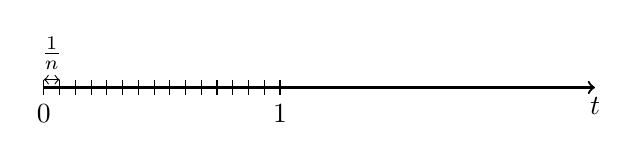
\begin{tikzpicture}
  \draw[->, thick] (5,0) -- (12,0) node[below] {\(t\)};
  % Optional: Add ticks and labels
  \foreach \x in {5,5.2,...,8}
    \draw (\x,0.1) -- (\x,-0.1);
    \node[below] at (5,-0.1) {0};
    \node[below] at (8,-0.1) {1};
    \draw[<->] (5,0.1) -- (5.2,0.1) node[midway, above] {\(\frac1n\)};
\end{tikzpicture}
\[X_1=\underbrace{X_1-X_{\frac{n-1}n}}_{Y_{n-1}}+\underbrace{X_{\frac{n-1}n}-X_{\frac{n-2}n}}_{Y_{n-2}}+\cdots+\underbrace{X_{\frac1n}-X_0}_{Y_0},X_0:=0\]
\(Y_0,Y_1,\ldots,Y_{n-1}\) nezavisne jednako distribuirane, \(\varphi_{Y_0}=\varphi_{X_1}^{1/n}\) \ding{51} može jer je \(X_1\) beskonačno djeljiva \ding{163}\newline Možemo nastaviti dalje na \([0,+\infty\rangle\): \(X_{\frac{k}n},k\in\Bbb N_0\) \ding{222} \(n\to+\infty\) i "profinjenje"; \[X_{\frac{k}n},n\in\Bbb N,k\in\Bbb N_0,\varphi_{X_{1/n}}=e^{\frac1n\psi}\Rightarrow\varphi_{X_{k/n}}=e^{\frac{k}n\psi}.\] Možemo li dobiti nešto u limesu? \begin{enumerate}
    \item[\ding{228}] L\'evy \ding{224} DA! Dobijemo familiju slučajnih varijabli \((X_t)_{t\ge0}\) t. d. vrijedi
    \item[\((i)\)] \(0\le t_0<t_1<\cdots<t_n\)\newline \(X_{t_1}-X_{t_0},\ldots,X_{t_n}-X_{t_{n-1}}\) su nezavisne (svojstvo nezavisnih prirasta)
    \item[\((ii)\)] \(\varphi_{X_{t+s}-X_t}=\varphi_{X_s}=e^{s\psi},s,t\ge0\) (svojstvo stacionarnih prirasta)\newline \(t=0\Rightarrow\varphi_{X_0}=e^0=1\Rightarrow X_0=0\) g. s.
\end{enumerate}
L\'evy je pokazao da iz svake beskonačno djeljive distribucije s karakterističnom funkcijom \(e^\psi,\) možemo vezati familiju \((X_t)_{t\ge0}\) s nezavisnim stacionarnim prirastima t. d. je \(\varphi_{X_t}=e^{t\psi},\forall t\ge0.\)\newline\newline
\ding{46}\textbf{NAPOMENA}\newline
Ovakva familija \((X_t)_{t\ge0}\) naziva se slučajan proces, a varijablu \(t\) interpretiramo kao vrijeme. Možeo promatrati preslikavanja:
\begin{enumerate}
    \item[\ding{228}] \(X:\Omega\times[0,+\infty\rangle\to\Bbb R,X(\omega,t):=X_t(\omega)\)
    \item[\ding{228}] slučajnu varijablu \(\omega\mapsto X_t(\omega)\)
    \item[\ding{228}] za fiksirani \(\omega\in\Omega, [0,+\infty\rangle\ni t\mapsto X_t(\omega)\) \ding{222} trajektorija (\textit{eng.} "sample path")
\end{enumerate}
Ovakav slučajan proces ima još jedno važno svojstvo:
\begin{enumerate}
    \item[\((iii)\)] \(t\searrow 0\Rightarrow\forall u\in\Bbb R,\varphi_{X_t}=\underbrace{e^{t\psi(u)}}_{\substack{\text{nepre-}\\\text{kidna}\\\text{funkcija}}}\to\varphi_{X_0}(u)\Rightarrow X_t\overset{\mathcal D}{\longrightarrow}0\) (const.) \(\Rightarrow X_t\overset{\Bbb P}{\longrightarrow}0\)\newline Fiksirajmo neki \(t>0\) i pustimo \(s\to t.\) \(\varphi_{X_s}(u)\to\varphi_{X_t}(u)\Rightarrow X_s\overset{\mathcal D}{\longrightarrow}X_t,\) ali može se pokazati i da \(X_s\overset{\Bbb P}{\longrightarrow}X_t\) 
\end{enumerate}
\(\Rightarrow\) slučajni proces koji je L\'evy realizirao neprekidan je po vjerojatnosti.\newline\newline
Okrenimo "kut gledanja".\newline
\textbf{DEFINICIJA}\newline
Slučajan proces \((X_t)_{t\ge0}\) jest proces s nezavisnim stacionarnim prirastima ako vrijedi \((i)\) te \[\forall t,s\ge0,X_{t+s}-X_t\sim X_s, X_0=0\text{ g. s.}\]
Mora li takav proces nastati iz beskonačno djeljive distribucije? Ne!\newline\newline
\textbf{PRIMJER} (čak deterministički):\newline
Ako imamo funkciju \(g(t),t\ge0\) t. d. je \(g(t+s)=g(t)+g(s),\forall t,s\ge0,\) onda će \(Y_t:=g(t)\) zadovoljavati gornju definiciju.\newline\newline 
Kako izgledaju rješenja te funkcionalne jednadžbe? Može se konstruirati proces koji zadovoljava ova svojstva, ali nije "pravac". Takav proces konstruira se pomoću aksioma izbora i daje funkciju koja nije neprekidna.\begin{enumerate}
    \item[\ding{228}] deterministički pravac \ding{222} drugo ponašanje na svakom. 
\end{enumerate} Takav pravac nije nastao ni iz jedne beskonačno djeljive distribucije.\newline\newline
\emph{Ideja}: zahtijevamo barem da je \(t\mapsto\varphi_{X_t}(u)\) neprekidna za svaki \(u.\) Uzmimo \(n\in\Bbb N.\) \[X_{\frac1n}-X_0+X_{\frac2n}-X_{\frac1n}+\cdots+X_1-X_{\frac{n-1}n}=X_1,\]\(X_{\frac1n}-X_0,X_{\frac2n}-X_{\frac1n},\ldots,X_1-X_{\frac{n-1}n}\) \[\Rightarrow X_1=\sum_{k=1}^nY_k\Rightarrow\varphi_{X_1}=\varphi_{Y_1}^n\;(\forall n\in\Bbb N)\;\Rightarrow\varphi_{X_1}\text{ je beskonačno djeljiva}\]
Svaki \(t\ge0\) može se aproksimirati racionalnim točkama \(\frac{k}n,\) pa iz ove neprekidnosti slijedi \[\frac{k_l}{n_l}\to t\Rightarrow\varphi_{X_{\frac{k_l}{n_l}}}\to\varphi_{X_t},\] a \[\varphi_{X_{\frac{k_l}{n_l}}}(u)=e^{\frac{k_l}{n_l}\psi(u)}\] pa, sveukupno, \[\Rightarrow\varphi_{X_t}(u)=e^{t\psi(u)}\]
Time je pokazano sljedeće:\newline
\textbf{TEOREM}\newline
\((X_t)_{t\ge0}\) je slučajan proces s nezavisnim stacionarnim prirastima t. d. je \(\forall u\in\Bbb R,t\mapsto\varphi_{X_t}(u)\) neprekidna \(\Leftrightarrow\) \((X_t)_{t\ge0}\) je nastao iz beskonačno djeljive razdiobe \(\varphi_{X_1}=e^\psi\) i \(\forall t\ge0,\varphi_{X_t}=e^\psi.\)\newline\newline
1-1 korespondencija \((X_t)_{t\ge0}\leftrightarrow e^\psi\) beskonačno djeljiva.\newline Npr. ako \(X_{t+s}-X_t\) ne ovisi o doga\dj{}ajimado trenutka \(t,\) proces ima i Markovljevo svojstvo. 
\newpage
\section{Brownovo gibanje - okvirno}
\ding{46}\textbf{NAPOMENA}\newline
Neka su \((X_t)_{t\ge0}\) i \((Y_t)_{t\ge0}\) slučajni procesi s vrijednostima u \(\Bbb R.\) Može se pokazati da je spomenuto preslikavanje \(X:\Omega\times[0,+\infty\rangle. X(\omega,t)=X_t(\omega)\) \(\left(\mathcal F\otimes B_{[0,+\infty\rangle},B_\Bbb R\right)\)-izmjerivo \emph{u smislu verzije}. Tako\dj{}er, \((X_t)_{\ge0}\) i \((Y_t)_{t\ge0}\) su jednako distribuirani \(\Leftrightarrow\) za svaki \(n\in\Bbb N\) i svaki izbor me\dj{}usobno različitih \(t_1,\ldots,t_n\in[0,+\infty\rangle,\) \((X_{t_1},\ldots,X_{t_n})\sim(Y_{t_1},\ldots,Y_{t_n}).\) Kad govorimo o "ovakvom procesu", zapravo govorimo o klasi jednako distribuiranih stohastičkih procesa. \((Y_t)_{t\ge0}\) je \emph{modifikacija} procesa \((X_t)_{t\ge0}\) ako je, za svaki \(t\ge0,X_t=Y_t\) g. s. Očito je da modifikacija \(\Rightarrow X_t\sim Y_t,\) no obrat ne vrijedi! \((X_t)_{t\ge0}\) i \((Y_t)_{t\ge0}\) su \emph{nerazlučivi} ako \(\exists A\in\mathcal F,\Bbb P(A)=0,\forall t\ge0,\forall\omega\in A^c,X_t(\omega)=Y_t(\omega).\) Ako su dva procesa nerazlučiva, onda je jedan modifikacija drugoga, no ne i obratno.\newline\newline
\emph{Što se doga\dj{}a s trajektorijom?}\newline
\(\omega\in\Omega,t\mapsto X_t(\omega),(\Bbb P)\lim\limits_{h\to0}X_{t+h}=X_t.\) Znamo da tada postoji podniz \(\left(X_{t+h_{p_n}}\right)\) t. d. \(X_{t+h_{p_n}}\overset{\text{g. s.}}{\longrightarrow}X_t.\)\newline\newline
\ding{46}\textbf{NAPOMENA}\newline Mogli bismo pomisliti da su možda gotovo sve trajektorije neprekine, no to je netočno!\newline\newline
\emph{cadlag}(continue \`{a} droite, limite \`{a} gauche) \[D\left([0,+\infty\rangle\right):=\left\{f:[0,+\infty\rangle\to\Bbb R\mid\; f\text{ je neprekidna zdesna i ima limes slijeva u svakoj točki }t\in[0,+\infty\rangle\right\}\] Može se pokazati da, za svaku \(e^\psi,\) postoji modifikacija originalnog procesa t. d. su gotovo sve trajektorije unutar \(D\left([0,+\infty\rangle\right).\) \((X_t)_{t\ge0}\leadsto\left(\tilde X_t\right)_{t\ge0}.\) Trivijalnim redefiniranjem procesa na skupu vjerojatnosti \(0,\) dolazimo do procesa \(\left(\tilde{\tilde X}_t\right)_{t\ge0}\) nerazlučivog od \(\left(\tilde X_t\right)_{t\ge0}\) čije su sve trajektorije u \(D\left([0,+\infty\rangle\right).\)\newline\newline
Uspostavili smo, dakle, korespondenciju \(e^\psi\) s procesom \((X_t)_{t\ge0}\) sa sljedećim svojstvima:
\begin{enumerate}
    \item[\((i)\)] \((X_t)_{t\ge0}\) je proces s nezavisnim stacionarnim prirastima.
    \item[\((ii)\)] \(\varphi_{X_t}=e^{t\psi}\)
    \item[\((iii)\)] \(\forall\omega\in\Omega,t\mapsto X_t(\omega)\in D\left([0,+\infty\rangle\right).\) 
\end{enumerate} Kažemo da je \((X_t)_{t\ge0}\) L\'evyjev proces generiran sa \(\psi.\)\newline\newline
\textbf{PITANJE}: jesu li i kada trajektorije ipak neprekidne? Prisjetimo se \(\psi=\psi_A+\psi_B,\) gdje je \(\psi_A(u)=iu\gamma-\frac{\sigma^2u^2}2,\) a \(\psi_B\) je definirana pomoću integrala. Ispostavlja se da funkcijom \(\psi_B\) dodajemo skokove, a u integralu je dana informacija o njihovoj distribuciji.\newline\newline
\textbf{TEOREM}\newline L\'evyjev proces generiran sa \(\psi\) ima modifikaciju kojoj su sve trajektorije neprekidne \(\Leftrightarrow\) \(\psi=\psi_A.\)\newline\newline
\textbf{TEOREM}\newline Za svaki \(\psi,\) postoje me\dj{}usobno nezavisni procesi \((X_t^A)_{t\ge0}\) s eksponentom \(\psi_A\) i \((X_t^B)_{t\ge0}\) s eksponentom \(\psi_B\) t. d. je eksponent od \(\left(X_t^A+X_t^B\right)_{t\ge0}\) \(\psi.\)\newline\newline
Pogledajmo proces generiran sa \(\psi_A(u)=iu\gamma-\frac{\sigma^2t^2}2,\sigma>0.\) [\(\sigma]\ge0,\) ali \(\sigma=0\Rightarrow X_t=\gamma t\) trivijalno]. \[\psi_{X_t}(u)=e^{t\psi_A(u)}\Rightarrow X_t=t\gamma+\sigma B_t, B_t\sim\psi(u)=-\frac{t^2}2.\] Po prethodnom teoremu, \((B_t)_{t\ge0}\) ima neprekidne trajektorije. \(\Rightarrow\) analiza \(\psi_A\) svodi se na analizu \((B_t)_{t\ge0}.\)\newline\newline \((B_t)_{t\ge0}\) je matematička generalizacija procesa u prirodi, poznat pod nazivom \textbf{Brownovo gibanje}.\newline\newline
\emph{Historijat}
\begin{enumerate}
    \item[\ding{228}] Antonie van Leeuwenhoek (1632.-1723.), izumitelj mikroskopa, "kaotično gibanje čestica promatranih u vodi"
    \item[\ding{228}] 1819., Bywater "neorganske supstance" (iziritirane)
    \item[\ding{228}] škotski botaničar Robert Brown (1773.-1858.)
    \item[\ding{228}] 1917. D'Arcy Thompson \emph{"žive ili ne?"}
    \item[\ding{228}] \(XIX\) st.  fizičari i kemičari
    \item[\ding{228}] Louis Bachelier
    \item[\ding{228}] Albert Einstein\begin{enumerate}
        \item[] \(p(y,t,t_0,x_0)\) \[\begin{aligned}p(t+s,y;t_0,x_0)&=\int_{-\infty}^{+\infty}p(t,u;t_0,x_0)p(s,y,t,u)du\\p(t+\delta,x)&=\int_{-\infty}^{+\infty}p(t,u)p(\delta,x-u)du,\;\;t_0=x_0=0\end{aligned}\] 
        \item[] postoji konstanta \(D,\) \[\lim_{\Delta t\to0}\frac1{\Delta t}\int_{-\infty}^{+\infty}x^kp(\Delta t,x)dx=\begin{cases}0,&k=1,3,4,5,\ldots\\D,&k=2\end{cases}\] Einstein zanemaruje više momente, naslućuje simetričnost
        \item[] jednadžba topline \[\begin{aligned}\frac{\partial p}{\partial t}&=D\left(\frac12\frac{\partial^2p}{\partial x^2}\right),p(0,x)=\delta_{\{x\}}\\p(t,x)&=\frac1{\sqrt{2\pi D t}}e^{-\frac{x^2}{2Dt}}\\D&=\frac{kT}{3\pi\eta a}=\frac{kT}{m\beta}2\end{aligned}\]
    \end{enumerate}
    \item[\ding{228}] Jean-Baptiste Perrin (1870.-1942.)\begin{enumerate}
        \item[\ding{93}] serija eksperimenata (broj udara u sekundi reda \(10^{20}\))
        \item[\ding{93}] 1926. Nobelova nagrada
    \end{enumerate}
    \item[\ding{228}] Norbert Wiener
\end{enumerate}
\textbf{DEFINICIJA}\newline
Stohastički proces \((B_t)_{t\ge0}\) na vjerojatnosnom prostoru \((\Omega,\mathcal F,\Bbb P)\) s vrijednostima u \(\Bbb R\) jest \textbf{standardno jednodimenzionalno Brownovo gibanje} ako vrijedi:
\begin{enumerate}
    \item[\((i)\)] \(B_0=0\)
    \item[\((ii)\)] \((B_t)_{t\ge0}\) je proces s nezavisnim stacionarnim prirastima
    \item[\((iii)\)] \(\forall t\ge0, B_t\sim N(0,t)\)
    \item[\((iv)\)] trajektorije \(t\mapsto B_t(\omega)\) su neprekidne za sve \(\omega\in\Omega.\)
\end{enumerate}
\begin{enumerate}
    \item[\ding{228}] Markovljevi procesi
    \item[\ding{228}] Feller \ding{224} jednodimenzionalne difuzije\begin{enumerate}
        \item[\ding{46}] Jaki Markovljevi procesi
        \item[\ding{46}] sve trajektorije neprekidne
    \end{enumerate}
    \item[\ding{228}] It\^o-McKeen \ding{224} teorija stohastičkih integrala
\end{enumerate}
Budući da je \(B_0=0, B_h\sim N(0,h^2)\) te da su prirasti nezavisni i stacionarni, \[\lim_{h\to 0^+}\Var\left(\frac{B_{t+h}-B_t}h\right)=\lim_{h\to0^+}\Var\left(\frac{B_h-B_0}h\right)=\lim_{h\to0^+}\Var\left(\frac{B_h}h\right)=\lim_{h\to0^+}\frac1h=+\infty\]
\textbf{TEOREM}\newline Gotovo sve trajektorije Brownovog gibanja nemaju nigdje derivaciju. (Dvoretsky, Erd\"{o}s, Kakutani)\newline\newline
Za gotovo sve trajektorije \[\begin{aligned}\underset{t\to\infty}{\lim\inf}B_t(\omega)&=-\infty\\\underset{t\to\infty}{\lim\sup}B_t(\omega)&=+\infty\end{aligned}\]
\begin{enumerate}
    \item[\ding{113}] broj prijelaza Brownovog gibanja kroz \(0\): \(\infty\) (kako se vrši dok se ne odvoji od \(0\)?)
    \item[\ding{113}] Hausdorffova dimenzija
    \item[\ding{113}] vrijeme zadržavanja u \(0\)
    \item[\ding{113}] lokalno vrijeme
    \item[\ding{113}] \(d\)-dimenzionalno Brownovo gibanje u \(\Bbb R^d\)\begin{enumerate}
        \item[\ding{96}] profinjenje slučajne šetnje
        \item[\ding{96}] \(X_t=(B_t^1,\ldots, B_t^d),\) pri čemu su \((B_t^1)_{t\ge0},\ldots,(B_t^d)_{t\ge0}\) standardna jednodimenzionalna Brownova gibanja i nezavisne komponente!
    \end{enumerate}
    \item[\ding{113}] u slučaju \(d=1,\) promatramo ograničen otvoreni skup \(D,\) to može biti i otvoren interval \(I\) oko nule, i pretpostavimo da je na \(\partial D\) definirana funkcija \(f.\) Tražimo funkciju \(u\) koja je rješenje od \[\begin{cases}\Delta u=0\text{ na }D\footnotemark[39]\\u_{\mid\partial D}=f\end{cases}\]\footnotetext[39]{Laplacian} Svakoj točki \(x\in D,\) možemo pridružiti \((X_t+x)_{t\ge0}\)-Brownovo gibanje koje počinje u \(x.\) Definirajmo \(\tau_x:=\inf\{t>0\mid X_t\in\partial D\}=\min\{t>0\mid X_t\in\partial D\}\) (jer je trajektorija neprekidna, a \(\partial D\) je kompaktan) i \(\Bbb E^x\left[f\left(X_{\tau_x}\right)\right]\)-srednja vrijednost tih udara. Ispostavlja se \(u(x)=\Bbb E\left[f\left(X_{\tau_x}\right)\right].\)
    \item[\ding{113}] u slučaju \(d=2,\) promatramo otvorenu kuglu . \((B_t)_{t\ge0}\) beskonačno mnogo puta vraća se u otvoreni krug \(I\) i to počevši od bilo kojeg trenutka \(\Rightarrow\) \emph{povratnost/rekurentnost}
    \item[\ding{113}] u slučaju \(d=3,\) promatramo otvorenu kuglu oko ishodišta. \(\Rightarrow\) \emph{prolaznost/tranzijentnost}
\end{enumerate}
\begin{center}
    \Huge{\textbf{KRAJ KOLEGIJA\ding{163}}}
\end{center}
\newpage
\section{Dodatak \(1\) (Brownovo gibanje - općenitije, svibanj \(2024.\))}
\subsection{Uvod} 
Neka su \((Y_n)_{n\in\Bbb N}\) nezavisne jednako distribuirane slučajne varijable, \(\Bbb EY_i=0,\Var Y_i=1,\) npr., \(Y_1\sim\begin{pmatrix}-1&1\\1/2&1/2\end{pmatrix}.\) Slučajna šetnja: \(S_0=0,S_n=Y_1+\cdots+Y_n,n\in\Bbb N.\) Kažemo da ima nezavisne priraste ako su za \(n,k\ge 0,\) \(S_n\) i \(S_{n+k}-S_n\) nezavisne. Induktivno su i \(S_{n_1},S_{n_2}-S_{n_1},\ldots,S_{n_k}-S_{n_{k-1}}\) nezavisne za \(n_1<n_2<\cdots<n_k.\) Fiksirajmo \(n\in\Bbb N\) i "ubrzajmo" slučajnu šetnju: \[S_t^{(n)}:=S_{nt},\text{ za }nt\in\Bbb Z_+,t\ge0.\] (Kao da ju suzimo, npr., na \([0,1]\)).
\begin{enumerate}
    \item[\ding{228}] linearno interpoliramo  za \(t>0,nt\notin\Bbb Z_+\) \[S_t^{(n)}=S_{\lfloor nt\rfloor}+\left(S_{\lfloor nt\rfloor+1}-S_{\lfloor nt\rfloor}\right)\left(nt-\lfloor nt\rfloor\right)=S_{\lfloor nt\rfloor}+Y_{\lfloor nt\rfloor+1}\left(nt-\lfloor nt\rfloor\right)\] 
    \item[] \(t=\frac{k}n\leadsto S_k+Y_{k+1}(nt-k)\)
    \item[] \(\Var S_1^{(n)}=\Var S_n=\sum_{k=1}^n\Var Y_k=n,\) što ne konvergira pa moramo skalirati.\newline \(\sqrt{\Var S_1^{(n)}}=\sqrt n\)
\end{enumerate}
\textbf{DEFINICIJA} \[B_t^{(n)}:=\frac1{\sqrt n}S_t^{(n)}=\frac1{\sqrt n}S_{\lfloor nt\rfloor}+\frac1{\sqrt n}Y_{\lfloor nt\rfloor+1}\left(nt-\lfloor nt\rfloor\right)\]
\begin{enumerate}
    \item[] \(\Var B_1^{(n)}=\Var\left(\frac1{\sqrt n}S_1^{(n)}\right)=\frac1n\Var S_n=1\) 
    \item[] \(B_1^{(n)}=\frac{S_1^{(n)}}{\sqrt n}=\frac{S_n}{\sqrt n}=\frac{Y_1+\cdots+Y_n}{\sqrt n}\overset{\mathcal D}{\longrightarrow}N(0,1)\)
    \item[] \(B_t^{(n)}\overset{\mathcal D}{\longrightarrow}N(0,t)\) (jer \(\sqrt{\frac{\lfloor nt\rfloor}n}\to\sqrt t,\) a \(\frac{nt-\lfloor nt\rfloor}{\sqrt n}\to0\) kad \(n\to\infty\))
\end{enumerate}
\subsection{Definicija i konačno-dimenzionalne distribucije}
\textbf{DEFINICIJA}\newline
Standardno jednodimenzionalno Brownovo gibanje jest slučajni proces \(B=(B_t)_{t\ge0}\) sa svojstvima:
\begin{enumerate}
    \item[\((i)\)] \(B_0=0\) g. s.
    \item[\((ii)\)] Za \(0\le t_1<\cdots<t_n,B_{t_1},B_{t_2}-B_{t_1},\ldots,B_{t_n}-B_{t_{n-1}}\) su nezavisne slučajne varijable. (\(B\) ima nezavisne priraste)
    \item[\((iii)\)] Za \(s,t\ge0,\) \(B_{s+t}-B_s\sim N(0,t)\)
    \item[\((iv)\)] Za g. s. \(\omega\in\Omega,\) \(t\mapsto B_t(\omega)\) je neprekidna funkcija.
\end{enumerate}
\textbf{ZADATAK}\newline
Neka je \(B=(B_t)_{t\ge0}\) slučajan proces t. d. vrijedi \((i),(ii)\) i \((iii).\)\newline\newline
\textit{Rješenje.} \[s,t\ge0, B_{s+t}=(B_{s+t}-B_s)+B_s\overset{\substack{\text{nez.}\\(ii)}}{\Rightarrow}\underbrace{\varphi_{B_{s+t}}(u)}_{e^{-\frac{(s+t)u^2}2}}=\varphi_{B_{s+t}-B_s}(u)\underbrace{\varphi_{B_s}(u)}_{e^{-\frac{su^2}2}}\Rightarrow\varphi_{B_{s+t}-B_s}(u)=e^{-\frac{tu^2}2}\Rightarrow B_{s+t}-B_s\sim N(0,t).\]
\textbf{ZADATCI}\newline
Neka je \(B=(B_t)_{t\ge0}\) Brownovo gibanje. Tada su Brownova gibanja i 
\begin{enumerate}
    \item[\((i)\)] \((-B_t)_{t\ge0}\)
    \item[\((ii)\)] Za \(s>0,\) \(X=(X_t)_{t\ge0},X_t:=B_{t+s}-B_s\) (\emph{invarijantnost na translaciju})
    \item[\((iii)\)] Za \(a>0,\) \(X=(X_t)_{t\ge0}, X_t:=\frac1{\sqrt a}B_{at}\)
    \item[\((iv)\)] \((B_1-B_{1-t})_{t\in[0,1]}\) (Brownovo gibanje na \([0,1]\)) (\emph{invarijantnost na skaliranje})
\end{enumerate}
Neka je \(0<t_1<t_2<\cdots<t_n.\) \(\left(B_{t_1},B_{t_2}-B_{t_1},\ldots,B_{t_n}-B_{t_{n-1}}\right)\) je normalan slučajan vektor s gustoćom \[g(x_1,\ldots,x_n)=g_{t_1}(x_1)g_{t_2-t_1}(x_2)\cdots g_{t_tn-_{n-1}}(x_n),\;g_t(x):=\frac1{\sqrt{2\pi t}}e^{-\frac{x^2}{2t}}\] i kovarijacijskom matricom \[\begin{bmatrix}t_1&&&\\&t_2-t_1&&\\&&\ddots&\\&&&t_n-t_{n-1}\end{bmatrix}.\]
Distribucija vektora \(\left(B_{t_1},\ldots,b_{t_n}\right):\) \[\begin{bmatrix}B_{t_1}\\B_{t_2}\\\vdots\\B_{t_n}\end{bmatrix}=\begin{bmatrix}1&&&&\\1&1&&&\\1&1&1&&\\\vdots&\vdots&\vdots&\ddots&\\1&1&1&\ldots&1\end{bmatrix}\begin{bmatrix}B_{t_1}\\B_{t_2}-B_{t_1}\\\vdots\\B_{t_n}-B_{t_{n-1}}\end{bmatrix},\] a kovarijacijska mu je matrica \(\begin{bmatrix}t_i\land t_j\end{bmatrix}_{i,j}.\)
\begin{enumerate}
    \item[\(s\le t\)] \(\Cov(B_s,B_t)=\Bbb E\left[B_sB_t\right]=\Bbb E\left[B_s\left(B_s+B_t-B_s\right)\right]\overset{\text{nez.}}{=}\Bbb E\left[B_s^2\right]+\underbrace{\Bbb EB_s}_0\Bbb E\left[B_t-B_s\right]=s=s\land t\) 
\end{enumerate}
\textbf{DEFINICIJA}\newline
Slučajni je proces \emph{gaussovski} ako su mu sve konačno-dimenzionalne distribucije normalne.\newline\newline
\textbf{PROPOZICIJA}\newline
Neka je \(B=(B_t)_{t\ge0}\) slučajan proces sa svojstvima:
\begin{enumerate}
    \item[\((a)\)] \(B_0=0\) g. s.
    \item[\((b)\)] \(B\) je gaussovski
    \item[\((c)\)] \(\forall s,t\ge0,\Bbb EB_s=0,\Cov(B_s,B_t)=s\land t\)
    \item[\((d)\)] = \((iv)\)
\end{enumerate}
Tada je \(B\) standardno jednodimenzionalno Brownovo gibanje. Vrijedi i obrat.\newline\newline
\textit{Dokaz.}
\begin{enumerate}
    \item[\(\boxed{\Leftarrow}\)]
    \item[\(\boxed{\Rightarrow}\)]\((a)\) \& \((c)\) \newline \((b)\) \& \((d)\) \(\Rightarrow\) \((B_{t_1},\ldots,B_{t_n})\) je normalan slučajan vektor s kovarijacijskom matricom \(\begin{bmatrix}t_i\land t_j\end{bmatrix}_{i,j}\) \[\left(B_{t_1},B_{t_2}-B_{t_1},\ldots,B_{t_n}-B_{t_{n-1}}\right)^T=A^{-1}\left(B_{t_1},\ldots,B_{t_n}\right)=A^{-1}\left(B_{t_1},\ldots,B_{t_n}\right)^T\] \[\Cov\left(\left(B_{t_1},B_{t_2}-B_{t_1},\ldots,B_{t_n}-B_{t_{n-1}}\right)^T\right)=\begin{bmatrix}t_1&&&&\\&t_2-t_2&&&\\&&\ddots&&\\&&&&t_n-t_{n-1}\end{bmatrix}\] Dakle, komponente su mu normalne i nekorelirane pa su i nezavisne.
\end{enumerate}
\textbf{TEOREM}\[\sum_{n=0}^\infty\Bbb P\left(\sup_{n\le t<n+1}|B_t-B_n|\ge n^{2/3}\right)<\infty.\]
\textit{Dokaz.}\newline
Neka je \(m\in\Bbb N.\) \(B_{n+2^{-m}}-B_n,B_{n+2\cdot 2^{-m}}-B_{n+2^{-m}},\ldots,B_{n+1}-B_{n+(2^m-1)2^{-m}}\) su nezavisne (podijelimo \([n,n+1]\) na \(2^m\) dijelova). \[\begin{aligned}\sum_{j=1}^k\left(B_{n+j2^{-m}}-B_{n+(j-1)2^{-m}}\right)&=B_{n+k2^{-m}}-B_n\\\overset{\substack{\text{Kolmogorovljeva}\\\text{maksimalna}\\\text{nejednakost}}}{\Rightarrow}\Bbb P\left(\sup_{q\le k\le2^m}\left|B_{n+k2^{-m}}-B_n\right|>n^{1/3}\right)&\le\frac1{n^{4/3}}\Bbb E\left[(B_{n+1}-B_n)^2\right]=\frac1{n^{4/3}}.\end{aligned}\] Budući da su trajektorije neprekidne, a dijadski razlomci gusti u \(\Bbb R,\) \[\begin{aligned}\left\{\sup_{n\le t\le n+1}|B_t-B_n|>n^{2/3}\right\}&=\bigcup_{m=1}^\infty\left\{\sup_{1\le k\le 3^m}\left|B_{n+k2^{-m}}-B_n\right|>n^{2/3}\right\}\\\Rightarrow\Bbb P\left(\sup_{n\le t\le n+1}|B_t-B_n|>n^{2/3}\right)&=\lim_{m\to\infty}\Bbb P\left(\sup_{1\le k\le 3^m}\left|B_{n+k2^{-m}}-B_n\right|>n^{2/3}\right)\le\frac1{n^{4/3}}\\\Rightarrow\sum_{n=0}^\infty\Bbb P\left(\sup_{n\le t\le n+1}|B_t-B_s|\ge n^{2/3}\right)\le 1+\sum_{n=1}^\infty\frac1{n^{4/3}}<+\infty\end{aligned}\] \textbf{POSLJEDICA} ovog teorema: Po Borel-Cantelli 1, \(\Bbb P\left(\sup_{n\le t\le n+1}|B_t-B_n|\ge n^{2/3}\text{ b. m. p.}\right)=0.\) \(\Rightarrow\) za g. s. \(\omega\in\Omega,\exists n_0=n_0(\omega)\in\Bbb N,\forall n\ge n_0,\sup\limits_{n\le t\le n+1}|B_t-B_s|<n^{2/3}\) \[\underset{t\to\infty}{\lim\sup}\frac{\left|B_t(\omega)-B_{\lfloor t\rfloor}(\omega)\right|}t\le\underset{t\to\infty}{\lim\sup}\sup_{n\le t\le n+1}\frac{|B_t(\omega)-B_n(\omega)|}t\le\underset{t\to\infty}{\lim\sup}\frac{\lfloor t\rfloor^{2/3}}t=0.\]
\textbf{PROPOZICIJA (Jaki zakon velikih brojeva za Brownovo gibanje)}\newline Neka je \(B=(B_t)_{t\ge0}\) standardno jednodimenzionalno Brownovo gibanje. Tada vrijedi \[\lim_{t\to\infty}\frac{B_t}t=0\text{ g. s.}\]
\textit{Dokaz.} \[\begin{aligned}\lim_{n\to\infty}\frac{B_n}n&=\lim_{n\to\infty}\frac{B_1+(B_2-B_1)+\cdots+(B_n-B_{n-1})}n\\\frac{B_t}t&=\underbrace{\frac{B_{\lfloor t\rfloor}}{\lfloor t\rfloor}}_{\to0}\underbrace{\frac{\lfloor t\rfloor}t}_{\to1}+\underbrace{\frac{B_t-B_{\lfloor t\rfloor}}t}_{\overset{\text{g. s.}}{\longrightarrow}0
}\end{aligned}\]
\textbf{ZADATAK}\newline
Neka je \(B=(B_t)_{t\ge0}\) standardno jednodimenzionalno Brownovo gibanje. Definiramo slučajni proces \(X=(X_t)_{t\ge0}\): \(X_0=0\) g. s. \(X_t=tB_{1/t},t>0.\) Tada je \(X\) standardno jednodimenzionalno Brownovo gibanje.\newline\newline
\textit{Rješenje.}
\begin{enumerate}
    \item[\((a)\)] iz definicije (prethodna propozicija)
    \item[\((b)\)] \((X_{t_1},X_{t_2},\ldots,X_{t_n})^T=(t_1B_{1/t_1},\ldots,t_nB_{1/t_n})^T=\begin{bmatrix}t_1&&\\&\ddots&\\&&t_n\end{bmatrix}\begin{bmatrix}B_{1/t_1}\\\vdots\\B_{1/t_n}\end{bmatrix},\) što je afina transformacija normalnog slučajnog vektora pa je opet normalan slučajan vektor.
    \item[\((c)\)] \(s\le t,\) \(\Cov(X_s,X_t)=\Cov(sB_{1/s},tB_{1/t})=st\Cov(B_{1/s},B_{1/t})=st\left(\frac1s\land\frac1t\right)=st\frac1t=s=s\land t\)
    \item[\((d)\)] za \(t>0:\) \(t\mapsto X_t=tB_{1/t}\) je produkt neprekidnih funkcija. A, za \(t=0,\) \[\lim_{t\to0}X_t=\lim_{t\to0}tB_{1/t}=\begin{bmatrix}s=\frac1t\end{bmatrix}=\lim_{s\to\infty}\frac{B_s}s\overset{\text{JZVB}}{=}0\text{ g. s.}\]
\end{enumerate}
\subsection{Egzistencija Brownovog gibanja}
Relativno je lagano pokazati da postoji slučajan proces sa svojstvima \((i),(ii)\) i \((iii):\) \(t>0x,y\in\Bbb R\) \[p_t(x,y)=g_t(y-x)=\frac1{\sqrt{2\pi t}}e^{-\frac{(y-x)^2}{3t}}\]
Za \(0<s<t<u,x,z\in\Bbb R\) \[\int_\Bbb Rp_{t-s}(x,y)p_{u-t}(y,z)dy=p_{u-s}(0,z),x<0\quad(\triangle)\] \[\left(B_t-B_s\right)+\left(B_u-B_t\right)=B_u-B_s.\] Gustoća zbroja nezavisnih slučajnih varijabli konvolucija je gustoća pribrojnika. \[\begin{aligned}\int_\Bbb Rf_{B_t-B_s}(y)f_{B_u-B_t}(z-y)dy&=f_{B_u-B_s}(z)\\\int_\Bbb R\frac1{\sqrt{2\pi(t-s)}}e^{-\frac{y^2}{2(t-s)}}\cdot\frac1{\sqrt{2\pi(u-t)}}e^{-\frac{(z-u)^2}{2(u-t)}}dy&=\frac1{\sqrt{2\pi(u-s)}}e^{-\frac{z^2}{2(u-s)}}\end{aligned}\] 
\begin{enumerate}
    \item[\ding{228}] \(\Bbb Q_2:=\left\{m2^{-n}\mid m,n\in\Bbb N_0\right\}\)-skup svih nenegativnih dijadskih razlomaka (gusti u \(\Bbb R_+\))
    \item[\ding{228}] \(\Omega_q:=\Bbb R^{\Bbb Q_2}=\left\{\text{ funkcije }\Bbb Q_2\to\Bbb R\right\}\)
    \item[\ding{228}] \(\mathcal F_q=\) cilindrična \(\sigma\)-algebra na \(\Omega_q\) \(=\sigma\left(\bigcup\limits_{\substack{n\in\Bbb N\\0<t_1<\cdots<t_n\\t_i\in\Bbb Q_2}}\pi^{-1}_{t_1,\ldots,t_n}\left(B_{\Bbb R^n}\right)\right)\)
\end{enumerate}
\textbf{Uniformna neprekidnost}
\begin{enumerate}
    \item[\ding{113}] \(\varepsilon>0,\) odaberemo \(\eta>0\) t. d. je \(\eta<\min\left\{\left(\frac\varepsilon{c}\right)^{1/\gamma},2^{-(1-\delta)N}\right\}\)
    \item[\ding{113}] \(r,q\in\Bbb Q_2\cap[0,1]\) t. d. \(|r-q|<\eta\)
\end{enumerate}
Tada \begin{enumerate}
    \item[\((i)\)] \(|r-q|<2^{-(1-\delta)N}\)
    \item[\((ii)\)] \(c|r-q|^\gamma<c\cdot\frac\varepsilon{c}=\varepsilon\)
\end{enumerate}
\[\Rightarrow|f(q)-f(r)|\le C|r-q|^\gamma<\varepsilon\Rightarrow f\text{ je uniformno neprekidna}\]
\textbf{Proširenje po neprekidnosti funkcije na \([0,1]\)}
\begin{enumerate}
    \item[\ding{113}] \(t\in[0,1],(q_n)_{n\in\Bbb N}\subseteq\Bbb Q_2\cap[0,1],q_n\overset{n\to\infty}{\longrightarrow}t\)
    \item[\ding{113}] \(|f(q_n)-f(q_m)|\le C|q_n-q_m|^\gamma\leadsto\) za dovoljno velike \(n,m\)
    \item[\(\Rightarrow\)] \((f(q_n))_{n\in\Bbb N}\) je Cauchyjev \(\Rightarrow\) \((f(q_n))_{n\in\Bbb N}\) konvergira
    \item[\ding{113}] \(f(t):=\lim\limits_{n\to\infty}f(q_n).\) \(s,t\in[0,1]\)
    \item[] \(|f(t)-f(s)|=\begin{bmatrix}r_n:=s\end{bmatrix}=\lim\limits_{n\to\infty}|f(q_n)-f(r_n)|\le C\lim\limits_{n\to\infty}|q_n-r_n|^\gamma=C|t-s|^\gamma\)
\end{enumerate}
\textbf{DEFINICIJA}\begin{enumerate}
    \item[\ding{113}] \(f:[0,+\infty\rangle\to\Bbb R\) je \emph{Lipschitz neprekidna} u točki \(t_0\ge0\) ako \(\exists\delta>0,\exists c>0,\forall t\in[0,+\infty\rangle,|t-t_0|<\delta\Rightarrow|f(t)-f(t_0)|\le C|t-t_0|\)
    \item[\ding{113}] \(f:[0,+\infty\rangle\) je \emph{Lipschitz neprekidna} ako  \(\exists c>0,|f(t)-f(s)|\le c|t-s|,\forall t,s\ge0.\) 
\end{enumerate}
Zbog \(m\ge N\) te \(j-i\le 2^{m\delta},\) iz pretpostavke \((\triangle),\) slijedi \[\left|f\left(j2^{-m}\right)-f\left(i2^{-m}\right)\right)|\le\left(2^{m\delta}2^{-m}\right)^\gamma=2^{-\gamma m(1-\delta)}\]
Po neprekidnosti, \[\begin{aligned}\left|f(q)-f\left(i2^{-m}\right)\right|&=\left|f\left(i2^{-m}-2^{-q(1)}-\cdots-2^{-q(k)}\right)-f\left(i2^{-m}\right)\right|\\&\le\sum_{p=1}^k\left|f\left(i2^{-m}-q^{-q(1)}-\cdots-2^{-q(p)}\right)-f\left(i2^{-m}-2^{-q(1)}-\cdots-2^{-q(p-1)}\right)\right|\le(\ast\ast)\end{aligned}\]\[\begin{aligned}\left|f\left(i2^{-m}-2^{-q(1)}-\cdots-2^{-q(p)}\right)-f\left(i2^{-m}-\cdots-2^{-q(p-1)}\right)\right|&=\left|f\left(i'2^{-q(p)}\right)-f\left((i'+1)2^{-q(p)}\right)\right|\\&\overset{(\triangle)}{\le}2^{-q(p)\gamma}\end{aligned}\]
\[\begin{aligned}(\ast\ast)&\le\sum_{\gamma=1}^k2^{-q(p)\gamma}\le\begin{bmatrix}q(p)>m+p\end{bmatrix}\le\sum_{p=1}^k2^{-(m+p)\gamma}\le\sum_{p=m}^\infty 2^{-p\gamma}=C_12^{-m\gamma}\\\Rightarrow\left|f(q)-f\left(i2^{-m}\right)\right|&\le C_12^{-\gamma m}\quad(\triangle\triangle\triangle)\\\left|f(r)-f\left(j2^{-m}\right)\right|&\le C_22^{-\gamma m}\quad(\triangle\triangle\triangle\triangle)\quad\text{(slično)}\\\Rightarrow|f(q)-f(r)|&\le\left|f(q)-f\left(i2^{-m}\right)\right|+\left|f\left(i2^{-m}\right)-f\left(j2^{-m}\right)\right|+\left|f\left(j2^{-m}\right)-f(r)\right|\\&\le C_12^{-m\gamma}+C_22^{-m\gamma}+2^{-\gamma m(1-\delta)}\le C_32^{-\gamma m(1-\delta)}\\&\le\begin{bmatrix}2^{-m(1-\delta)}=2^{-(m+1)(1-\delta)}\cdot2^{1-\delta}\le(r-q)2^{1-\delta}\end{bmatrix}\le C_32^{1-\delta}(r-q)\end{aligned}\]
\textbf{PROBLEM} \[C:=\left\{\omega\in\Omega\mid t\mapsto\omega(t)\text{ je neprekidna funkcija}\right\}\] Po svojstvu \((iv)\leadsto\nu(C)=1,\) ali, ispostavlja se da \(C\notin\mathcal F_0.\) Po Kolmogorovljevom teoremu proširenja, postoji jedinstvena vjerojatnosna mjera na \((\Omega_q,\mathcal F_q)\) t. d. \(\nu\left(\{\omega\mid\omega(0)=0\}\right)=1\) i vrijedi \[\nu\left(\left\{\omega\mid\omega(t_i)\in A_i,0<t_1<\cdots<t_n\right\}\right)=\mu_{t_1,\ldots,t_n}(A_1\times\cdots\times A_n),t_i\in\Bbb Q_2.\]
\textbf{LEMA}\newline Neka je \(f:\Bbb Q_2\to\Bbb R,\gamma,\delta>0.\) Pretpostavimo da \(\exists N\in\Bbb N,\forall n\in\Bbb N,\) vrijedi \[\left|f\left(j2^{-n}\right)-f\left(i2^{-n}\right)\right|\le\left((j-i)2^{-n}\right)^\gamma,\forall 0\le i,j\le 2^n\text{ t. d. }0<j-i<2^{n\delta}.\] Tada \(\exists c>0,\forall r,q\in\Bbb Q_2\cap [0,1]\) t. d. \(0<r-q<2^{-(1-\delta)N}\) vrijedi \(|f(q)-f(r)|\le c|r-q|^\gamma.\) Posebno, \(f\) je uniformno neprekidna na \(\Bbb Q_2\cap[0,1].\)\newline\newline
\textit{Dokaz.}\newline Neka su \(r,q\in\Bbb Q_2\cap[0,1],0<r-q<2^{-(1-\delta)N},m\in\Bbb N\) t. d. \(2^{-(m+1)(1-\delta)}\le r-q<2^{-m(\gamma-\delta)}.\;(\ast).\) Neka je \(j\) najveći indeks t. d. je \(j2^{-m}\le r.\) \(\Rightarrow r=j2^{-m}+2^{-r(1)}+\cdots+2^{-r(l)},m<r(1)<\cdots<r(l).\) Slično, neka je \(i\) najmanji indeks t. d. \(i2^{-m}\ge q.\) \(\Rightarrow q=i2^{-m}-2^{-q(1)}-\cdots-2^{-q(k)},m<q(1)<\cdots<q(k).\) \[\Rightarrow r-q=(j-i)2^{-m}+2^{-r(1)}+\cdots+2^{-r(l)}+2^{-q(1)}+\cdots+2^{-q(k)}<2^{-m(1-\delta)}\Rightarrow(j-i)2^{-m}\le 2^{-m(1-\delta)}/\cdot 2^m\Rightarrow j-i\le 2^{m\delta}\]
\begin{enumerate}
    \item [] \(\begin{cases}X_t=tB_{1/t},t>0\\X_0=0\end{cases}\)
    \item[\ding{228}] Kad Brownovo gibanje izlazi iz \(0,\) beskonačno mnogo puta pogodi \(0\)
    \item[\ding{228}] to vrijedi za svako Brownovo gibanje (svojstvo distribucije Brownovog gibanja)
\end{enumerate}
\begin{enumerate}
    \item[\ding{113}] \(0<t_1<t_2<\cdots<t_n,n\in\Bbb N.\) Na \(\left(\Bbb R^n,B_{\Bbb R^n}\right)\) definiramo vjerojatnosnu mjeru \[\mu_{t_1,\ldots,t_n}(A_1\times\cdots\times A_n)=\int_{A_1}dx_1\int_{A_2}dx_2\cdots\int_{A_n}dx_n\prod_{m=1}^np_{t_m,t_{m-1}}(x_{m-1},x_m).\] Zbog \((\triangle),\) ta je familija vjerojatnosnih mjera SUGLASNA. \[t_{n+1}>t_n,\quad\mu_{t_1,\ldots,t_{n+1}}(A_1\times\cdots\times A_n\times\Bbb R)=\mu_{t_1,\ldots,t_n}(A_1\times\cdots\times A_n)\] 
    \item[\ding{228}] \(\Omega_0:=\Bbb R^{[0,+\infty\rangle}=\left\{f:[0,+\infty\rangle\to\Bbb R\right\}\)
    \item[\ding{228}]  \(\mathcal F_0=\sigma\left(\bigcup_{\substack{n\in\Bbb N\\0<t_1<\cdots<t_n}}\pi^{-1}_{t_1,\ldots,t_n}\left(B_{\Bbb R^n}\right)\right)\)
\end{enumerate}
Iz Kolomogorovljevog teorema o proširenju, slijedi\newline\newline
\textbf{TEOREM}\newline Postoji jedinstvena vjerojatnost \(\nu\) na \((\Omega_0,\mathcal F_0)\) t. d. \(\nu\left(\left\{\omega\mid \omega(0)=0\right\}\right)=1\) i \[\nu\left(\left\{\omega\mid\omega(t_i)\in A_i,0<t_1<\cdots<t_n\right\}\right)=\mu_{t_1,\ldots,t_n}(A_1\times\cdots\times A_n).\] Stavimo \(X_t(\omega)=\omega(t).\) Tada \((X_{t_1},\ldots,X_{t_n})\) ima distribuciju \(\mu_{t_1,\ldots,t_n},\) tj., normalnu distribuciju - centriranu, s kovarijacijskom matricom \(\begin{bmatrix}t_i\land t_j\end{bmatrix}_{i,j}.\)\newline\newline Dakle, našli smo prostor i proces koji zadovoljava \((i)-(iii).\)\newline\newline
\textbf{TEOREM}\newline
Neka je \(f:[0,+\infty\rangle\to\Bbb R\) diferencijabilna u \(t_0\ge0.\) Tada je \(f\) Lipschitz neprekidna u \(t_0.\)\newline\newline
\ding{46}\textbf{NAPOMENA}\newline Obrat ne vrijedi! Npr., \(f(x)=|x|.\)\newline\newline
\textbf{DEFINICIJA}\newline
\(f:[0,+\infty\rangle\to\Bbb R\) je \emph{H\"older neprekidna} u \(t_0\ge0\) s eksponentnom \(\alpha>0\) ako \(\exists\delta>0,\exists c>0,\forall t\in[0,+\infty\rangle,|t-t_0|<\delta\Rightarrow|f(t)-f(t_0)|\le C|t-t_0|^\alpha.\)\newline\newline
\ding{46}\textbf{NAPOMENA}\newline Ako je \(f\) H\"older neprekidna s eksponentom \(\alpha>0,\) onda je H\"older neprekidna i s eksponentom \(\beta>\alpha,\forall \beta>\alpha.\)\newline\newline
\textbf{TEOREM}\newline 
Neka je \(T<+\infty.\) Tada je \(\nu\)-g. s.  \(\omega:\Bbb Q_2\to\Bbb R\) uniformno neprekidna na \(\Bbb Q_2\cap[0,2].\)\newline\newline
\textit{Dokaz.}\newline
BSOMP \(T=1.\) Neka je \(\Bbb P:=\nu, B_t-B_s\sim  N(0,t-s),0\le s<t,s,t\in\Bbb Q_2.\)\newline \(\Bbb E\left[(B_t-B_s)^4\right]=3(t-s)^2\leadsto\Bbb E\left[(B_t-B_s)^4\right]\le C(t-s)^2.\)\newline \(\gamma<\frac14,\delta>0.\) Markovljeva nejednakost: \(a^4\Bbb P(|X|>a)\le\Bbb E\left[|X|^4\right]\) \[\begin{aligned}{}&{\color{white}=}\Bbb P\left(\left|B_{j2^{-n}}-B_{i2^{-n}}\right|>\left((j-i)2^{-n}\right)^\gamma\text{ za neke }0\le i,j<2^n\text{ t. d. }0<j-i<2^{n\delta}\right)\\&=\Bbb P\left(\bigcup_{\substack{0\le i,j\le 2^n\\0<j-i<2^{n\delta}}}\left\{\left|B_{j2^{-n}}-B_{i2^{-n}}\right|>\left((j-i)2^{-n}\right)^\gamma\right\}\right)\\&\le\sum_{\substack{0\le i,j\le 2^n\\0<j-i<2^{n\delta}}}\Bbb P\left(\left|B_{j2^{-n}}-B_{i2^{-n}}\right|>\left((j-i)2^{-n}\right)^\gamma\right)\overset{\text{Markov}}{\le}\sum_{\substack{0\le i,j\le 2^n\\0<j-i<2^{n\delta}}}\left((j-i)2^{-n}\right)^{-4\gamma}\Bbb E\left[\left|B_{j2^{-n}}-B_{i2^{-n}}\right|^4\right]\\&\le\sum_{\substack{0\le i,j<2^n\\0<j-i<2^{n\delta}}}\left((j-i)2^{-n}\right)^{-4\gamma}C\left((j-i)2^{-n}\right)^2\le C\sum_{\substack{0\le i,j\le 2^n\\0<j-i<2^{n\delta}}}\left((j-i)2^{-n}\right)^{-4\gamma+2}\\&\le\begin{bmatrix}\#\text{ sumanada }\le 2^n\cdot 2^{n\delta}\\\text{ jer je }i\in\{0,\ldots,2^n-1\},j<2^{n\delta}+i\end{bmatrix}\\&\le C\cdot 2^n\cdot 2^{n\delta}\cdot\left(2^{n\delta}2^{-n}\right)^{-4\gamma+2}=C2^{-n(-1-\delta+(4\gamma-2))\delta-4\delta+2)}\\&=\begin{bmatrix}\varepsilon:=(2-4\delta)(1-\delta)-(1+\delta)>0\\2-4\gamma>0\Rightarrow\exists\delta>0,\varepsilon>0\end{bmatrix}\\\Rightarrow&\sum_{n\in\Bbb N}\Bbb P\left(\left|B_{j2^{-n}}-B_{i2^{-n}}\right|>\left((j-i)2^{-n}\right)^\gamma\text{ za neke }0\le i,j\le 2^n,0<j-i<2^{n\delta}\right)\le C\sum_{n\in\Bbb N}2^{-n\varepsilon}<\infty\end{aligned}\] Po Borel-Cantelli 1, za g. s. \(\omega\in\Omega_q,\exists N(\omega)\in\Bbb N\) t. d.  \[\forall n\ge N(\omega),\left|B_{j2^{-n}}(\omega)-B_{i2^{-n}}(\omega)\right|\le \left((j-i)2^{-n}\right)^\gamma,\forall 0\le i,j<2^n,0<j-i<2^{n\delta}.\] Po Lemi, slijedi neprekidnost na \([0,1],\) tj., postoji neprekidno proširenje.\newline\newline 
\(\leadsto\) g. s. \(\omega\) se može proširiti do uniformno neprekidne, štoviše do  \(\gamma\)-H\"older neprekidne s eksponentom \(\frac14,\) na svakom \([0,T]\) \(\Rightarrow\) sveukupno, može se proširiti do uniformno neprekidne (\(\gamma\)-H\"older neprekidne na \([0,+\infty\rangle\)) \[(\boxed{})\Bbb E\left[|B_t-B_s|^\beta\right]\le C|t-s|^{1+\alpha}\]
\begin{enumerate}
    \item[\ding{228}] u dokazu prethodnog teorema, umjesto \({}^{-4},\) pišemo  \(-\beta,\) umjesto \(\gamma,\) pišemo \(1+\alpha\)
    \item[\ding{228}] \(\ldots\) isti način \(\varepsilon=(1+\alpha-\beta\gamma)(1-\delta)-(1+\delta)\)
    \item[\(\leadsto\)] uniformna neprekidnost vrijedi \(\forall\gamma,1+\alpha-\beta\gamma>0,\) tj., ?? \(\forall\gamma<\frac\alpha\beta\)
    \item[\ding{228}] \(C_m=\Bbb E\left[|B_1|^{2m}\right]\overset{\text{skaliranje}}{\longrightarrow}\overset{\substack{\text{momenti}\\\text{normalne}\\\text{razdiobe}}}{\Bbb E\left[|B_t-B_s|^{2m}\right]}\le C_m|t-s|^m\)
    \item[\ding{113}] \(\beta=2m,\alpha=m-1\)\newline ??\(\forall\gamma<\frac12,\exists m,\gamma<\frac{m-1}{2m}=\frac\alpha\beta\)
\end{enumerate}
\textbf{POANTA}\newline Zapravo je \(\forall\gamma<\frac12,\) a ne \(\gamma<\frac14\) \(\gamma\)-H\"older neprekidna\newline\newline-------------------------------------------------------------------------------------------------------
\begin{enumerate}
    \item[\ding{228}] Izmjeriv prostor \((C,\mathcal C)\)
    \item[\ding{228}] \(C\) - neprekidne funkcije \([0,+\infty\rangle\to\Bbb R\)
    \item[\ding{228}] \(\mathcal C\) - cilindrična \(\sigma\)-algebra (generirana projekcijama \(\pi_t:C\to\Bbb R,\pi_t(\omega)=\omega(t)\))
\end{enumerate}
\textbf{DEFINICIJA}  \[\Psi:\Omega_q\to C\]
\(\Psi(\omega):=\) neprekidno proširenje of \(\omega\) s \(\Omega_q\) na \([0,+\infty\rangle\)\newline \(\to\) ako je \(\omega\) iz skupa \(\nu\)-vjerojatnosti \(1,\) funkcija je \(\equiv0\) i na ??\newline\newline
\textbf{LEMA}\newline
\(\Psi\) je \((\mathcal F_q,\mathcal C)\)-izmjeriva.\newline\newline
\textit{Dokaz.}\newline
Dovoljno je pokazati da \(\Psi\) dobro invertira skupove iz neke generirajuće familije za \(\mathcal C.\) \[\left\{\tilde\omega\in C\mid\tilde\omega(t_1)\in A_1,\ldots,\tilde\omega(t_n)\in A_n\right\},A_1,\ldots,A_n\subseteq\Bbb R\text{ otvoreni}.\] Neka je \({\color{YellowOrange}t}>0,A\subseteq\Bbb R\) otvoren. \[\Psi^{-1}\left(\left\{\tilde\omega\in C\mid\tilde\omega({\color{YellowOrange}t})\in A\right\}\right)=\left\{\omega\in\Omega_q\mid \Psi(\omega)({\color{YellowOrange}t})\in A\right\}=\left\{\omega\in\Omega_q\mid\lim\limits_{\substack{q_n\to {\color{YellowOrange}t}\\q_n\in\Bbb Q}}\omega(q_n)\in A\right\}=\bigcup_{n=1}^\infty\bigcap_{m=n}^\infty\left\{\omega(q_m)\in A\right\}\in\mathcal F_q.\]
Konačno, definirajmo vjerojatnost \(\Bbb P\) na \((C,\mathcal C):\) \(\boxed{\Bbb P:=\nu\circ\Psi^{-1}}\) te \(B_t:C\to\Bbb R,B_t(\omega):=\omega(t).\)\newline 
\textbf{TVRDNJA}\newline \(B=(B_t)_{t\ge0}\) Brownovo gibanje na vjerojatnosnom prostoru \((C,\mathcal C,\Bbb P).\)\newline\newline
\textit{Dokaz.}\newline Svojstva \((i)\) i \((iv)\) slijede po definiciji. Dokažimo \((iii).\) Neka su \(s,t\ge0.\) Ako su \((q_n)_{n\in\Bbb N},(r_n)_{n\in\Bbb N}\) t. d. \(q_n\to s+t,r_n\to t,\) zbog neprekidnosti trajektorija, slijedi \(B_{s+t}=\lim\limits_{n\to\infty}B_{q_n},B_s=\lim\limits_{n\to\infty}B_{r_n}\) i \[B_{t+s}-B_s=\lim_{n\to\infty}\underbrace{(B_{q_n}-B_{r_n})}_{\substack{\overset{\Bbb P}{\sim}N\left(0,q_n-r_n\right)\\\overset{\mathcal D}{\longrightarrow}N(0,t-s)}}\text{ g. s.}\]
\ding{96}\textbf{POANTA:} Postoji Brownovo gibanje \ding{163}\newline\newline
\textbf{PROPOZICIJA}\newline
Neka je \(t_0\ge0.\) Za g. s. \(\omega\in\Omega,\) putovi \(t\mapsto B_t(\omega)\) nisu Lipschitz-neprekidni u \(t_0.\)\newline\newline
\textit{Dokaz.}\newline
Definirajmo \(A_{t_0}:=\left\{\omega\in\Omega\mid t\mapsto B_t\text{ je Lipschitz-neprekidna u }t_0\right\}.\) Neka je \(\omega\in A_{t_0}.\) \(\exists\delta=\delta(\omega)>0,\exists c=c(\omega)>0,|t-t_0|<\delta\Rightarrow\left|B_t(\omega)-B_{t_0}(\omega)\right|\le C|t-t_0|.\) Neka je \(n\in\Bbb N\) t. d. \(\frac1{2^n}<\delta;m\in\Bbb N,m\ge c.\) \[\forall j\ge n,\left|\left(t_0+2^{-j}-t_0\right)\right|=2^{-j}<\delta\Rightarrow\left|B_{t_0+2^{-j}}(\omega)-B_{t_0}(\omega)\right|\le C\left|\left(t_0+2^{-j}\right)-t_0\right|\le m2^{-j}\] \[\Rightarrow\omega\in A_{m,n}:=\left\{\left|B_{t_0+2^{-j}}-B_{t_0}\right|\le m2^{-j},\forall j\ge n\right\}=\bigcap_{j=n}^\infty\left\{\left|B_{t_0+2^{-j}}-B_{t_0}\right|\le m2^{-j}\right\}\Rightarrow A_{t_0}\subseteq\bigcup_{m,n=1}^\infty A_{m,n}.\]
Nadalje, \(A_{n,m}\subseteq\left\{\left|B_{t_0+2^{-l}}-B_{t_0}\right|\le m2^{-l}\right\},\forall l\ge n\) kao presjek takvih. \[\begin{aligned}\Bbb P\left(\left|B_{t_0+2^{-l}}-B_{t_0}\right|\le 2^{-l}\cdot m\right)&=\begin{bmatrix}\text{stacionarnost}\\\text{prirasta}\end{bmatrix}=\Bbb P\left(\left|B_{2^{-l}}\right|\le m2^{-l}\right)=\begin{bmatrix}B_t\sim\sqrt tB_1\end{bmatrix}\\&=\Bbb P\left(\sqrt{2^{-l}}|B_1|\le m2^{-l}\right)=\Bbb P\left(|B_1|<m2^{-l/2}\right)\end{aligned}\]
\[\forall l\ge n,\Bbb P(A_{n,m})\le\Bbb P\left(\left|B_{t_0+2^{-l}}-B_{t_0}\right|\le 2^{-l}m\right)=\Bbb P\left(|B_1|\le m2^{-l/2}\right)\overset{l\to\infty}{\longrightarrow}0,\forall m,n\in\Bbb N\] \[\overset{\text{neprekidnost}}{\Rightarrow}\Bbb P\left(\bigcup_{m,n=1}^\infty A_{m,n}\right)=0\Rightarrow\Bbb P(A_{t_0})=0.\] \(\Rightarrow\) Lipschitz-neprekidne na doga\dj{}aju vjerojatnosti \(0.\)\newline\newline
\textbf{TEOREM}\newline
Neka je \(B=(B_t)_{t\ge0}\) Brownovo gibanje na \((\Omega,\mathcal F,\Bbb P).\) Za g. s. \(\omega\in\Omega,\) putovi \(t\mapsto B_t(\omega)\) nisu Lipschitz-neprekidni ni u jednoj točki \(t\ge0.\) Posebno, g. s. putovi \(t\mapsto B_t(\omega)\) nigdje nisu diferencijabilni.\newline\newline
\textit{Dokaz.}\newline
Definirajmo \(A:=\left\{\omega\in\Omega\mid\exists s\in[0,1],t\mapsto B_t(\omega)\text{ Lipschitz-neprekidna u }s \right\}.\) Neka je \(c>0.\) Za \(n\in\Bbb N,\) definirajmo \(\tilde A_n:=\left\{\omega\in\Omega\mid\exists s\in[0,1],|t-s|<\frac3n\Rightarrow|B_t(\omega)-B_s(\omega)|\le c|t-s|\right\}.\) Neka je \(n\ge3,k\in\{1,\ldots,n-2\}\) te \[\begin{aligned}Y_{k,n}:&=\max_{j=0,1,2}\left\{\left|B_{(k+j)/n}-B_{(k+j-1)/n}\right|\right\}\\\tilde B_n:&=\left\{\text{ barem jedan }Y_{k,n}\le\frac{5c}n\right\}=\bigcup_{k=1}^{n-2}\left\{Y_{k,n}\le\frac{5c}n\right\}.\end{aligned}\] Pokažimo da je \(\tilde A_n\subseteq\tilde B_n.\) Neka je \(\omega\in\tilde A_n.\) Tada \(\exists s\in[0,1]\) t. d. je \(|B_t(\omega)-B_t(s)|\le c|t-s|\) za \(|t-s|<\frac3n.\)
\begin{enumerate}
    \item[\(s=1\)] (najgora mogućnost) \[\begin{aligned}\left|B_{\frac{n-2}n}(\omega)-B_{\frac{n-3}n}(\omega)\right|&\le\underbrace{\left|B_{\frac{n-2}n}(\omega)-B_1(\omega)\right|}_{\le c\frac2n}+\underbrace{\left|B_1(\omega)-B_{\frac{n-3}n}(\omega)\right|}_{c\frac3n}\le\frac{5c}n\\\left|B_{\frac{n-1}n}(\omega)-B_{\frac{n-2}n}(\omega)\right|&\le\underbrace{\left|B_{\frac{n-1}n}(\omega)-B_1(\omega)\right|}_{\le c\frac1n}+\underbrace{\left|B_1(\omega)-{\frac{n-2}n}\right|}_{c\frac2n}<\frac{5c}n\\\left|B_{\frac{n-2}n}(\omega)-B_{\frac{n}n}(\omega)\right|&\le c\frac1n<\frac{5c}n\\\Rightarrow Y_{n-2,n}(\omega)&\le\frac{5c}n\Rightarrow\omega\in\tilde B_n\end{aligned}\] 
    \item[\(s<1\)] Tada \(\exists k\in\{1,\ldots,n-2\}\) t. d. se \(s\) nalazi negdje izme\dj{}u točaka \(\frac{k-1}n,\frac{k}n,\frac{k+1}n,\frac{k+2}n\) i, opet, rapisujući \(\left|B_{\frac{k+j}n}-B_s\right|+\left|B_s-B_{\frac{k+j-1}n}\right|\) (za koje ima smisla gledati), vidim da taj zbroj ne prelazi \(\frac{5c}n.\) Dakle, i u ovom slučaju, \(\omega\in\tilde B_n.\)  
\end{enumerate}
Dalje, \[\begin{aligned}\Bbb P\left(Y_{k,n}\le\frac{5c}n\right)&=\Bbb P\left(\left|B_{\frac{k}n}-B_{\frac{k-1}n}\right|\le\frac{5c}n,\left|B_{\frac{k+1}n}-B_{\frac{k}n}\right|\le\frac{5c}n,\left|B_{\frac{k+2}n}-B_{\frac{k+1}n}\right|\le\frac{5c}n\right)\\&=\begin{bmatrix}\text{nezavisnost}+\\\text{stacionarnost}\end{bmatrix}=\Bbb P\left(\left|B_{\frac1n}\right|\le\frac{5c}n\right)^3=\begin{bmatrix}B_{\frac1n}\sim\sqrt{\frac1n}B_1\end{bmatrix}\\&=\Bbb P\left(|B_1|\le 5cn^{-1/2}\right)^3=\left(\int_{-\frac{5c}n}^{\frac{5c}n}\frac1{\sqrt{2\pi}}e^{-\frac{x^2}2}dx\right)^3\le\left(\frac1{\sqrt{2\pi}}\cdot\frac{10c}{\sqrt n}\right)^3\\\Rightarrow\Bbb P\left(\tilde B_n\right)&\le\sum_{k=1}^{n-2}\Bbb P\left(Y_{k,n}\le\frac{5c}n\right)\le (n-2)\cdot(2\pi)^{-3/2}\cdot 10^3\cdot c^3\cdot n^{-3/2}\le(2\pi)^{-3/2}\cdot10^3\cdot c^3\cdot n^{-1/2}.\end{aligned}\] Neka je \(n\in\Bbb N.\) Definirajmo sada \(A_n:=\left\{\omega\in\Omega\mid\exists s\in[0,1],|B_t(\omega)-B_s(\omega)|\le n^{1/12}|t-s|\right\}\) (\(c=n^{1/12}\)) te \[B_n:=\left\{\text{ barem jedan }Y_{k,n}\le\frac{5n^{1/12}}n\right\}\;??\]
Prema pokazanome, vrijedi \(\Bbb P(B_n)\le(2\pi)^{-3/2}10^3n^{3/12-1/2}=(2\pi)^{-3/2}10^3n^{-1/4}.\)\newline \(A_1\subseteq A_2\subseteq\cdots\) Pokažimo da je \(A\subseteq\bigcup_{n=1}^\infty A_n.\) Neka je \(\omega\in A.\) Tada \(\exists s\in[0,1],\exists\delta>0,\exists c>0,|t-s|<\delta\Rightarrow|B_t(\omega)-B_s(\omega)|\le c|t-s|.\) Neka je \({\color{NavyBlue}n}\in\Bbb N\) t. d. \(\frac3{\color{NavyBlue}n}<\delta,{\color{NavyBlue}n}^{1/12}\ge c.\) Tada je \(\omega\in A_{\color{NavyBlue}n}.\) \[\begin{aligned}\underset{n\to\infty}{\lim\sup}A_n&=\left\{A_n\text{ b. m. p.}\right\}=\begin{bmatrix}\text{neopadajući}\\\text{doga\dj{}aji}\end{bmatrix}=\bigcup_{n=1}^\infty A_n=\bigcup_{n=1}^\infty A_{2^n}\\\sum_{n=1}^\infty\Bbb P\left(B_{2^n}\right)&\le(2\pi)^{-3}10^3\sum_{n=1}^\infty\left(2^n\right)^{-1/4}<+\infty\\\overset{\substack{\text{Borel}\\\text{Cantelli-}1}}{\Rightarrow}\Bbb P\left(B_{2^n}\text{ b. m. p.}\right)&=0.\end{aligned}\] No, \[A\subseteq\bigcup_{n=1}^\infty A_{2^n}=\left\{A_{2^n}\text{ b. m. p.}\right\}\subseteq\left\{B_{2^n}\text{ b. m. p.}\right\}\Rightarrow\Bbb P(A)=0.\]
\subsection{Funkcije ograničene varijacije}
Neka je \(f:[0,+\infty\rangle\to\Bbb R,t>0.\Delta=\{0=t_0<t_1<\cdots<t_n=t\}.\) Definiramo \[V^\Delta(t;f):=\sum_{i=1}^n|f(t_i)-f(t_{i-1})|.\] Ako je \(\Delta'\supseteq\Delta\) profinjenje od \(\Delta,\) \(V^{\Delta'}(t;f)\ge V^\Delta(t;f).\)\newline\newline
\textbf{DEFINICIJA}\newline
\textbf{Varijacija} funkcije \(f\) na \([0,t]\) je \[V(t)=V(t;f):=\sup_\Delta V^\Delta(t;f)\le+\infty.\]
\begin{enumerate}
    \item[\ding{113}] \(V(t)<+\infty,\) \(f\) je \emph{ograničene varijacije na \([0,t]\)}
    \item[\ding{113}] \(f\) je \emph{ograničene varijacije} ako je \(\forall t>0,V(t)<+\infty.\)
\end{enumerate}
\textbf{LEMA}\newline
Za \(0\le s<t\) vrijedi \(V(t)\ge V(s)+|f(t)-f(s)|.\)\newline\newline
\textit{Dokaz.}
\[\begin{aligned}\Delta&=\{0=t_0<\cdots<t_n=s\}\\\tilde\Delta&=\{0=t_0<\cdots<t_n<t_{n+1}=t\}=\Delta\cup\{t\}\\V^{\tilde\Delta}(t;f)&=V^\Delta(s;f)+|f(t)-f(s)|\bigg/\sup_{\Delta_{[0,t]}}\\\Rightarrow V(t;f)&\ge V^\Delta(s;f)+|f(t)-f(s)|\bigg/\sup_{\Delta_{[0,s]}}\\\Rightarrow V(t;f)&\ge V(s;f)+|f(t)-f(s)|\end{aligned}\]
Neka je \(f:[0,+\infty\rangle\to\Bbb R\) ograničene varijacije i neprekidna zdesna.
\begin{enumerate}
    \item[\ding{228}] \(V^+\to\mu_1,V^-\to\mu_2\) neopadajuće i neprekidne zdesna \[\Rightarrow V=V^++V^-\to\mu=\mu_1+\mu_2;f\to\mu_1-\mu_2\]
    \item[\ding{228}] \(\int_0^tg(s)dB_s(\omega)\leadsto\) sama teorija mjere, tj., integracije, ne dopušta! Tj., ne dopušta po trajektorijama jer nisu ograničene varijacije.\
   \item[\(\Rightarrow\)] ali, može se (financijsko modeliranje...)
\end{enumerate}
\subsection{Kvadratna varijacija Brownovog gibanja}
Neka je \(B=(B_t)_{t\ge0}\) Brownovo gibanje na \((\Omega,\mathcal F,\Bbb P).\) Za \(\Delta=\{0=t_0<t_1<\cdots<t_n=t\},\) definiramo \[\begin{aligned}Q^\Delta(t;B):&=\sum_{i=1}^n\left(B_{t_i}-B_{t_{i-1}}\right)\\|\Delta|:&=\max_{1\le i\le n}|t_i-t_{i-1}|\leadsto\text{ dijametar particije}\end{aligned}\]
Neka je
\begin{enumerate}
    \item[\ding{228}] \(\varphi[0,+\infty\rangle\to\Bbb R^d\) neprekidna funkcija,
    \item[\ding{228}] \(V^\Delta(t;f)=\sum_{i=1}^n\left\|\varphi(t_i)-\varphi(t_{i-1)}\right\|\)
    \item[\ding{228}] \(\underbrace{\int_0^t\|\varphi'(s)\|ds}_{\substack{\text{duljina}\\\text{luka}}}=V(t;\varphi)=\sup\limits_\Delta V^\Delta(t;\varphi)<+\infty\) (\(\varphi\) rektifibilna)
\end{enumerate}
\textbf{TEOREM (Lebesgue)}(bez dokaza)\newline
Neka je \(f:[0,+\infty\rangle\to\Bbb R\) neopadajuća funkcija. Tada je \(f\) diferencijabilna \(\lambda\)-g. s.\newline\newline
\textbf{POSLJEDICA}
\begin{enumerate}
    \item[\(\Rightarrow\)] funkcije ograničene varijacije diferencijabilne su \(\lambda\)-g. s.
    \item[\(\Rightarrow\)] trajektorije Brownovog gibanja \underline{nisu} ograničene varijacije  (jer nisu diferencijabilne g. s.) 
\end{enumerate}
Neka je \(F:[0,+\infty\rangle\to[0,+\infty\rangle\)  neopadajuća i neprekidna zdesna
\begin{enumerate}
    \item[\ding{228}] \(\mu\left(\langle a,b]\right):=F(b)-F(a)\)
    \item[\ding{228}] postoji jedinstveno proširenje od \(\mu\) na \(B_\Bbb R.\)
    \item[\ding{228}] \(1-1\) \(F\leftrightarrow\mu_F\)
    \item[\ding{228}] \(t\mapsto V(t)\) je neopadajuća funkcija
    \item[\ding{228}] \(0<s<t\): \[[V(t)\pm f(t)]-[V(s)\pm f(s)]=V(t)-V(s)\pm[f(t)-f(s)
    ]\ge V(t)-V(s)-|f(t)-f(s)|\overset{\text{LEMA}}{\ge}0.\] 
\end{enumerate}
Definiramo \emph{pozitivnu} i \emph{negativnu varijaciju} funkcije \(f\): \[\begin{matrix}V^+(t)=\frac{V(t)+f(t)}2&V^-(t):=\frac{V(t)-f(t)}2\end{matrix}\] \[\begin{aligned}\Rightarrow f(t)&=V^+(t)-V^-(t)\\V(t)&=V^+(t)+V^-(t)\end{aligned}\] funkcija ograničene varijacije razlika je dviju neopadajućih funkcija. Vrijedi i obrat.\newline\newline
Neka je \(f:[0,1]\to\Bbb R\) neopadajuća. Tada je \(f\) ograničene varijacije. Ako je, dodatno, \(f(0)=0, V(t;f)=f(t).\)\newline\newline
\textbf{PRIMJER}\newline Neka je \(f:[0,+\infty\rangle\to\Bbb R\) klase \(C^1\) na \([0,t],\forall t\ge0.\) Tada je \(f\) ograničene varijacije. \[V^\Delta(t;f)=\sum_{i=1}^n\underbrace{|f(t_i)-f(t_{i-1})|}_{\substack{|f(\xi_i)|(t_i-t_{i-1})\\\le\|f'\|_{\infty,t}(t_i-t_{i-1})}}\le\sum_{i=1}^n\|f'\|_{\infty,t}(t_i-t_{i-1})=t\|f'\|_{\infty,t}\Rightarrow V^\Delta(t;f)\le t\|f'\|_{\infty,t}<+\infty.\]
\begin{enumerate}
    \item[] \(\Bbb E Q^\Delta(t;B)=\sum_{i=1}^n\underbrace{\Bbb E\left[\left(B_{t_i}-B_{t_{i-1}}\right)^2\right]}_{t_i-t_{i-1}}=t\) 
    \item[] \(\Bbb E\left[\left(Q^\Delta(t;B)-t\right)^2\right]=\Var Q^\Delta(t;B)=\begin{bmatrix}\text{nezavisnost}\\\text{prirasta}\end{bmatrix}=\sum_{i=1}^n\Var\left(B_{t_i}-B_{t_{i-1}}\right)^2=(\ast)\)
    \item[\(0<s<t\):] \(\Var\left(B_t-B_s\right)^2=\Bbb E\left[\left((B_t-B_s)^2-(t-s)\right)^2\right]=\Bbb E\left[(B_t-B_s)^4\right]-2(t-s)\Bbb E\left[(B_t-B_s)^2\right]+(t-s)^2,\) a kako je \(B_t-B_s\sim N(0,\sigma^2)\) te \(Z\sim N(0,\sigma^2)\Rightarrow\Bbb E\left[Z^4\right]=3\sigma^4,\) to je jednako \(3(t-s)^2-2(t-s)^2+(t-s)^2=2(t-s)^2\)
    \item[] \((\ast)=\sum_{i=1}^n2\underbrace{\left(t_i-t_{i-1}\right)^2}_{\le|\Delta|}\le2|\Delta|\sum_{i=1}^n(t_i-t_{i-1})^=2t|\Delta|.\)
\end{enumerate}
\textbf{TEOREM}\newline
Neka je \((\Delta_k)_{k\in\Bbb N}\) niz particija segmenta \([0,t]\) t. d. \(|\Delta_k|\overset{k\to\infty}{\longrightarrow}0.\) Tada je \[\begin{aligned}\lim_{k\to\infty}Q^{\Delta_k}(t;B)=t\text{ u }L^2(\Omega,\mathcal F,\Bbb P),\text{ tj., }\\\lim_{k\to\infty}\Bbb E\left[\left(Q^{\Delta_k}(t;B)-t\right)^2\right]&=0\text{ (dokazano u gornjem razmatranju)}.\end{aligned}\] Pretpostavimo nadalje da je \(\lim\limits_{k\to\infty}k^2|\Delta_k|=0.\) Tada je \[\lim\limits_{k\to\infty}Q^{\Delta_k}(t;B)=t\text{ g. s.}\]
\textit{Dokaz \(2.\) tvrdnje:} \[\begin{aligned}\Bbb P\left(\left(Q^{\Delta_k}(t;B)-t\right)^2>2k^2|\Delta_k|\right)&\overset{\text{Markov}}{\le}\frac{\Bbb E\left[\left(Q^{\Delta_k}(t;B)-t\right)^2\right]}{2k^2|\Delta_k|}\le\frac{\cancel{2}\cancel{|\Delta_k|}t}{\cancel{2}k^2\cancel{|\Delta_k|}}=\frac{t}{k^2}\\\Rightarrow\sum_{k=1}^n\Bbb P\left(\left(Q^{\Delta_k}(t;B)-t\right)^2>2k^2|\Delta_k|\right)&\le\sum_{k=1}^n\frac{t}{k^2}<+\infty\\\overset{\substack{\text{Borel-}\\\text{Cantelli-1}}}{\Rightarrow}\Bbb P\left(\left(Q^{\Delta_k}(t;B)-t\right)^2>2k^2|\Delta_k|\text{ b. m. p.}\right)&=0\\\Rightarrow\left(Q^{\Delta_k}(t;B)-t\right)^2&\to0\text{ g. s.}\end{aligned}\] 
\begin{enumerate}
    \item[\ding{113}] \(0\le s<t,\Delta=\{s=t_0<\cdots<t_n=t\}\) \[\Bbb E\left[\left(\sum_{i=1}^n\left(B_{t_i}-B_{t_{i-1}}\right)^2-(t-s)\right)^2\right]\overset{|s|\to0}{\longrightarrow}0.\] 
    \item[\ding{113}] \textbf{POANTA}: Kvadratna varijacija Brownovog gibanja na svakom segmentu jednaka je \(t\)!
\end{enumerate}
\subsection{Nultočke Brownovog gibanja}
Neka je \(B=(B_t)_{t\ge0}\) Brownovo gibanje na \((\Omega,\mathcal F,\Bbb P).\) \(\exists\Omega_0\in\mathcal F,\Bbb P(\Omega_0)=1\) t. d. ako za \(\omega\notin\Omega_0\) redefiniramo  \(B_t(\omega)=0\) [nešto bude neprekidno... upotpuni bilješke]. Zanima nas skup \[\begin{aligned}\mathcal Z:&=\{(t,\omega)\in[0,+\infty\rangle\times\Omega\mid B_t(\omega)=0\}\\\text{prerez }\leftarrow\mathcal Z(\omega):&=\{t\ge0\mid B_t(\omega)=0\}\end{aligned}\]
\textbf{LEMA}\newline
Preslikavanje \((t,\omega)\mapsto B_t(\omega)\) s \([0,+\infty\rangle\times\Omega\) u \(\Bbb R\) jest \(\left(B_{[0,+\infty\rangle}\times\mathcal F, B_\Bbb R\right)\)-izmjerivo.\newline\newline
\textit{Dokaz.}\newline 
Neka je \(n\in\Bbb N.\) \(B_t^{(n)}(\omega):=\sum_{k=0}^\infty\mathbbm 1_{\left[\frac{k}n,\frac{k+1}n\right\rangle}(t)B_{\frac{k}n}(\omega).\) Zbog neprekidnosti trajektorija, \(B_t(\omega)=\lim\limits_{n\to\infty}B_t^{(n)}(\omega),\forall t\ge0,\forall\omega\in\Omega.\) \textcolor{Cyan}{[[Zbilja, \(\forall n\in\Bbb N,\exists! k\in\Bbb N,t\in\left[\frac{k}n,\frac{k+1}n\right\rangle,\frac{k+1}n-\frac{k}n=\frac1n\overset{n\to\infty}{\longrightarrow}0\) i nizom \(\left(\frac{k(t,n)}n\right)_{n\in\Bbb N}\) aproksimiramo \(t.\)]]} \(B_t^{(n)}\) je izmjeriva kao suma izmjerivih produkata, a onda je još i limes izmjerivih izmjerivo preslikavanje. \[\Rightarrow\mathcal Z= B^{-1}(\{0\})\in B_{[0,+\infty\rangle}\times\mathcal F.\] \(\Rightarrow Z_\omega\in B_{[0,+\infty\rangle}\) je zatvoren kao praslika zatvorenog \(\{0\}\) po neprekidnoj funkciji  \(t\mapsto B_t(\omega).\)\newline\newline
\textbf{KOROLAR}\newline
Za g. s. \(\omega\in\Omega,\) trajektorije \(t\mapsto B_t(\omega)\) beskonačne su varijacije na svakom intervalu.\newline\newline
\textit{Dokaz.}\newline
\(\exists\Omega_0\in\mathcal F,\Bbb P(\Omega_0)=1\) t. d. za svaki par racionalnih brojeva \(p<q,\) postoji niz particija \((\Delta_k)_{k\in\Bbb N}\) segmenta \([p,q],\) \(|\Delta_k|\overset{k\to\infty}{\longrightarrow}0\) \[\lim_{k\to\infty}\sum_{t_i\in\Delta_k}\left(B_{t_i}(\omega)-B_{t_{i-1}}(\omega)\right)^2=q-p,\forall\omega\in\Omega_0.\] 
Neka je \(V(\omega)\le+\infty\) varijacija funkcije \(t\mapsto B_t(\omega)\) na \([p,q].\) Vrijedi \[\begin{aligned}\sum_i\left(B_{t_i}(\omega)-B_{t_{i-1}}(\omega)\right)^2&\le\sup_i\left|B_{t_i}(\omega)-B_{t_{i-1}}(\omega)\right|\sum_i\left|B_{t_i}(\omega)-B_{t_{i-1}}(\omega)\right|\\&\le\underbrace{\left(\sup_i\left|B_{t_i}(\omega)-B_{t_{i-1}}(\omega)\right|\right)}_{\substack{\overset{k\to\infty}{\longrightarrow0}\\(\text{neprekidnost}\\\text{trajektorije})}}\underbrace{V(\omega)}-{\text{ako }<+\infty}\overset{|\Delta|\to 0}{\longrightarrow}0.\end{aligned}\] Dakle, na segmentu  \([p,q]\) je \(V(\omega)=+\infty\)\newline\newline
\textbf{KOROLAR}\newline
Trajektorije Brownovog gibanja su g. s. nigdje H\"older-neprekidne za \(\gamma>\frac12.\)\newline\newline
\textit{Dokaz.}\newline
Pretpostavimo da je \(|B_t(\omega)-B_s(\omega)|\le c|t-s|^\gamma,p\le s,t\le q,p,q\in\Bbb Q_+,\gamma>\frac12.\) Tada je \[\sum_i\left(B_{t_i}(\omega)-B_{t_{i-1}}(\omega)\right)^2\le c^2\sum_i\left|t_i-t_{i-1}\right|^{2\gamma}\le c^2\sup_i|t_i-t_{i-1}|^{2\gamma-1}\sum_i(t_i-t_{i-1})=c^2(q-p)\sup_i|t_i-t_{i-1}|^{2\gamma-1}\bigg/\lim_{|\Delta|\to0}\]
\textbf{DEFINICIJA/PODSJETNIK}
\begin{enumerate}
    \item[\ding{228}] Neka je \(A\subseteq[0,+\infty\rangle.\) Kažemo da je \(t\in[0,+\infty\rangle\) gomilište skupa \(A\) ako postoji niz \((t_n)_{n\in\Bbb N}\subseteq A\setminus\{t\}\) t. d. \(t=\lim\limits_{n\to\infty}t_n\) 
    \item[\ding{228}] \(t\in A\) je \emph{izolirana točka} skupa \(A\) ako \underline{nije} gomilište skupa \(A.\) \emph{Alternativno}, ako \(\exists\varepsilon>0,A\cap\langle t-\varepsilon,t+\varepsilon\rangle=\{t\}\)
    \item[\ding{228}] Kažemo da je skup \emph{perfektan} ako je jednak skupu svojih gomilišta.\begin{enumerate}
        \item[\ding{113}] Pokazuje se da je svaki perfektan skup neprebrojiv.  
    \end{enumerate}
\end{enumerate}
Neka je \(0\le q\in\Bbb Q_+.\) Definiramo \(d_{\color{Cyan}q}:=\inf\{t>{\color{Cyan}q}\mid B_t=0\}.\)\begin{enumerate}
    \item[\ding{113}] \((B_{d_q+t})_{t\ge0}\) je standardno Brownovo gibanje. (\ding{91}) \newline (Kad do\dj{}emo iz \(0,\) ponaša se kao standardno Brownovo gibanje.) Ovo nećemo dokazivati, ali točno je.
    \item[\ding{113}] \(q_1\le q_2\Rightarrow d_{q_1}\le d_{q_2}.\)
\end{enumerate}
\textbf{TEOREM}\newline
Za \(\Bbb P\)-g. s. \(\omega\in\Omega,\) skup \(\mathcal Z_\omega\)
\begin{enumerate}
    \item[\((i)\)] ima Lebesgueovu mjeru \(0\)
    \item[\((ii)\)] je zatvoren  i neome\dj{}en
    \item[\((iii)\)] ima gomilište u \(t=0\)
    \item[\((iv)\)] nema izoliranih nultočaka
\end{enumerate}
\textit{Dokaz.}
\begin{enumerate}
    \item[\((i)\)] Neka je \(\lambda\) Lebesgueova mjera na \([0,+\infty\rangle.\) \(\mathbbm 1_\mathcal Z(t,\omega)\) je izmjeriva (jer je \(\mathcal Z\) izmjeriv) \[\Bbb E\left[\lambda(\mathcal Z_\omega)\right]=(\lambda\times\Bbb P)(\mathcal Z)=\int_\Omega\int_{[0,+\infty\rangle}\mathbbm 1_\mathcal Z(t,\omega)d\lambda(t)d\Bbb P(\omega)=\int_{[0,+\infty\rangle}\underbrace{\int_\Omega\mathbbm 1_\mathcal Z(t,\omega)d\Bbb P(\omega)}_{\Bbb P(B_t=0)=0}d\lambda(t)=0\] \(\Rightarrow\Bbb E\left[\lambda(\mathcal Z_\omega)\right]=0\Rightarrow\lambda(\mathcal Z_\omega)=0\) za g. s. \(\omega\in\Omega.\)
    \item[\((ii)\)] \begin{enumerate}
        \item[\ding{228}] zatvorenost \ding{51} 
        \item[\ding{228}] neome\dj{}enost \(\leftarrow\)\begin{enumerate}
            \item[] \(\underset{t\to\infty}{\lim\sup}\frac{B_t}{\sqrt t}=+\infty\):\newline\newline Ponovimo: za niz \((X_n)_{n\in\Bbb N}\) nezavisnih jednako distribuiranih slučajnih varijabli s očekivanjem \(0\) i varijancom \(1,\) vrijedi \[\underset{n\to\infty}{\lim\sup}\frac{S_n}{\sqrt n}=+\infty\text{ g. s.}\] [[Neka je \(K>0\) proizvoljan. Tada je \[\begin{aligned}\Bbb P\left(\frac{S_n}{\sqrt n}\ge K\text{ b. m. p.}\right)&=\Bbb P\left(\bigcap_{n=1}^\infty\bigcup_{m=n}^\infty\left\{\frac{S_m}{\sqrt m}\ge K\right\}\right)=\lim\limits_{n\to\infty}\Bbb P\left(\bigcup_{m=n}^\infty\left\{\frac{S_m}{\sqrt m}\ge K\right\}\right)\\&\ge\lim\limits_{n\to\infty}\Bbb P\left(\frac{S_n}{\sqrt n}\ge K\right)\overset{\text{CGT}}{=}\Phi(-K)>0\end{aligned}\] Nadalje, \[\underset{n\to\infty}{\lim\sup}\frac{S_n}{\sqrt n}\ge K\Leftrightarrow\underset{n\to\infty}{\lim\sup}\frac{S_n-S_{n_0}}{\sqrt n}\ge K,\forall n_0\in\Bbb N\quad\left(\text{ jer }\forall n_0\in\Bbb N,\lim_{n\to\infty}\frac{S_{n_0}}{\sqrt n}=0\right)\] \(S_n-S_{n_0}\in\sigma(X_{n_0+1},X_{n_0+2},\ldots),\forall n_0\in\Bbb N\Rightarrow\left\{\underset{n\to\infty}{\lim\sup}\frac{S_n-S_{n_0}}{\sqrt n}\ge K\right\}\in\sigma(X_{n_0+1},X_{n_0+2},\ldots),\forall n_0\in\Bbb N,\) tj., \underline{repni je doga\dj{}aj} pa znamo da je vjerojatnosti \(0\) ili \(1.\) Zbog \[0<\Bbb P\left(\frac{S_n}{\sqrt n}\ge K\text{ b. m. p.}\right)\le\Bbb P\left(\underset{n\to\infty}{\lim\sup}\frac{S_n}{\sqrt n}\ge K\right),\] slijedi \(\Bbb P\left(\underset{n\to\infty}{\lim\sup}\frac{S_n}{\sqrt n}\right)=1\Rightarrow\underset{n\to\infty}{\lim\sup}\frac{S_n}{\sqrt n}\ge K\) g. s. \(\forall K>0\Rightarrow\underset{n\to\infty}{\lim\sup}\frac{S_n}{\sqrt n}=+\infty\) g. s.]] \(B_1,B_2-B_1,\ldots,B_n-B_{n-1}\) nezavisne su i jednako distribuirane s \(N(0,1)\)-razdiobom, dakle, očekivanjem \(0\) i varijancom \(1,\) \(B_n=B_1+(B_2-B_1)+\cdots+(B_n-B_{n-1})\) pa, po spomenutom rezultatu, \[\underset{t\to+\infty}{\lim\sup}\frac{B_t}{\sqrt t}\ge\underset{n\to\infty}{\lim\sup}\frac{B_n}{\sqrt n}=+\infty\text{ g. s.}\]
            \item[] \(\underset{t\to\infty}{\lim\inf}\frac{B_t}{\sqrt t}=-\infty\) 
        \end{enumerate}(mora beskonačno mnogo puta proći kroz \(0\)) 
    \end{enumerate}
    \item[\((iii)\)]\begin{enumerate}
        \item[] \(\underset{t\to0}{\lim\sup}\frac{B_t}{\sqrt t}=+\infty\)
        \item[] \(\underset{t\to0}{\lim\inf}\frac{B_t}{\sqrt t}=-\infty\)
    \end{enumerate} \(\Rightarrow\forall\varepsilon>0, B_t\) ima nultočku na \([0,\varepsilon].\)
    \item[\((iv)\)] Nužno je i dovoljno dokazati da je svaka točka iz \(\mathcal Z_\omega\) gomilište skupa \(\mathcal Z_\omega.\) \((iii)\) \& (\ding{91}) \(\Rightarrow\) \(B_{d_q}\) je g. s. gomilište skupa \(\mathcal Z_\omega.\) \begin{enumerate}
        \item[\(\Rightarrow\)] \(\{\omega\in\Omega\mid d_q(\omega)\text{ je izolirana točka u }\mathcal Z_\omega\}\) je \(\Bbb P\)-zanemariv.
        \item[\(\Rightarrow\)] \(N:=\bigcup_{q\in\Bbb Q_+}\{d_q\text{ je izolirana točka u }\mathcal Z\}\) je \(\Bbb P\)-zanemariv.
    \end{enumerate}
    Neka je \(h\in\mathcal Z_\omega.\) Tvrdimo da \(h\) nije izolirana.\newline Neka je \((q_n)_{n\in\Bbb N}\subseteq\Bbb Q\) t. d. \(q_n\nearrow h.\) Dvije su mogućnosti:\begin{enumerate}
        \item[\(1^\circ\)] \(h=d_{q_n}\) za neki \(n\in\Bbb N\)\newline Zbog \(h\ge d_{q_{n+k}}\ge\cdots\ge d_{q_n},k\ge 1,\) slijedi \(h=d_{q_k},\forall k\ge n.\)
        \item[\(2^\circ\)] \(h\ne d_{q_n},\forall n\in\Bbb N.\) Tada je \(q_1<d_{q_1}\le q_2<d_{q_2}<\cdots\le h\) pa je \(h=\lim\limits_{n\to\infty}d_{q_n}\) (točke izme\dj{}u točaka niza, a \(h\) je nultočka). \(h\) je opet gomilište (a još je i limes vremena zaustavljanja, premda ono samo to \emph{nije})
    \end{enumerate}
\end{enumerate}
\newpage
\section{Dodatak \(2\)}
\textbf{LEMA (Ottaviani\footnote[40]{Giuseppe Ottaviani} - Skorohod\footnote[41]{Skorohod, Anatolij Vladimirovič, 10. rujna 1930., Dnjepropetrovsk', SSSR - 3. siječnja 2011., Lansing, Michigan, SAD})}\newline Neka je \((X_n)_{n\in\Bbb N}\) niz \textbf{nezavisnih} slučajnih varijabli , \(\displaystyle S_n:=\sum_{k=1}^nX_k,n\in\Bbb N,x,y>0.\)\newline Ako je \(\displaystyle\beta:=\max_{1\le k\le n}\Bbb P\left(|S_n-S_k|>y\right)<1,\) tada \[\Bbb P\left(\max_{1\le k\le n}|S_k|>x+y\right)\le\frac1{1-\beta}\Bbb P(|S_n|>x|).\]
\textit{Dokaz.}\newline Definirajmo \[\begin{aligned}A:&=\left\{\max_{1\le k\le n}|S_k|>x+y\right\}\\A_k:&=\left\{\max_{1\le j\le k-1}|S_j|\le x+y,|S_k|>x+y\right\}.\\A&=\bigcup_{k=1}^n A_k\\(A_k)_{k=1}^n&\text{ su u parovima disjunktni}.\end{aligned}\] \[\begin{aligned}\Bbb P\left(|S_n|>x\right)&\ge\Bbb P\left(\left\{|S_n|>x\right\}\cap A\right)\\&=\sum_{k=1}^n\Bbb P\left(\left\{|S_n|>x\right\}\cap A_k\right)\\&=\sum_{k=1}^n\Bbb P\left(|S_n|>x,\max_{1\le j\le k-1}|S_j|\le x+y,|S_k|>x+y\right)\\&=\begin{bmatrix}|S_k|\le|S_n|+|S_k-S_n|\Rightarrow |S_n|\ge|S_k|-|S_n-S_k|\end{bmatrix}\\&\ge\sum_{k=1}^n\left(\left\{|S_n-S_k|\le y\right\}\cap A_k\right)\\&=\begin{bmatrix}\left\{|S_n-S_k|\le y\right\}\in\sigma\left(X_{k+1},\ldots,X_n\right),A_k\in\sigma\left(X_1,\ldots,X_k\right)\end{bmatrix}\\&=\sum_{k=1}^n\Bbb P\left(|S_n-S_k|\le y\right)\Bbb P(A_k)\\&=\sum_{k=1}^n\left(1-\Bbb P\left(|S_n-S_k|>y\right)\right)\Bbb P(A_k)\\&\ge(1-\beta)\sum_{k=1}^n\Bbb P(A_k)\\&=(1-\beta)\Bbb P(A)\\&=(1-\beta)\Bbb P\left(\max_{1\le k\le n}|S_k|>x+y\right)\end{aligned}\]
\newpage
\section{Dodatak \(3\)}
\textbf{PROPOZICIJA (dovoljan uvjet napetosti)}\newline
Ako postoji \(f:\Bbb R\to[0,+\infty\rangle\) t. d. je \(\displaystyle\lim_{|x|\to+\infty}f(x)\) i \(\displaystyle C:=\sup_n\int fd\Bbb P_n<+\infty,\) tada je niz \((\Bbb P_n)_{n\in\Bbb N}\) \textbf{napet}.\newline\newline
\textit{Dokaz.}\newline
Po definiciji, \(\displaystyle\forall M,\exists K>0, f(x)>M,\forall |x|\ge K\Rightarrow\inf_{|x|\ge K}f(x)\ge M>0.\) Dakle, sigurno \(\displaystyle\exists M>0,\inf_{|x|\ge M}f(x)>0.\) \[\begin{aligned}\Rightarrow C&\ge\int fd\Bbb P_n\ge\int_{\left\{|x|\ge M\right\}}fd\Bbb P_n\ge\left(\inf_{|x|\ge M}f\right)\int_{\left\{|x|\ge M\right\}}d\Bbb P_n=\left(\inf_{|x|\ge M}f\right)\Bbb P_n\left(\langle -M,M\rangle^c\right)\\\Rightarrow\Bbb P_n\left(\langle -M,M\rangle^c\right)&\le\frac{C}{\inf\limits_{|x|\ge M}f}.\end{aligned}\] Za \(\varepsilon>0,\) odaberemo \(M>0\) t. d. je \(\dfrac{C}{\inf\limits_{|x|\ge M}f}<\varepsilon\) (možemo jer, kako \(f(x)\to+\infty\) za velike \(x,\) \(\inf\) se može proizvoljno povećati).\newline\newline
\textit{Dokaz} (prof. Vondračeka) napetosti niza vjerojatnosnih mjera u dokazu Teorema neprekidnosti\newline\newline
Za dani \(\varepsilon>0,\) treba naći dovoljno mali \(u>0\) t. d. je \(\Bbb P_{X_n}\left(\left\{x\mid |x|>\frac2u\right\}\right)=\Bbb P_{X_n}\left(\Bbb R\setminus\left\langle-\frac2u,\frac2u\right\rangle\right)\) uniformno malo (po \(n\in\Bbb N\)) (za \(\varepsilon>0\) naći \(u\) t. d. je dana vjerojatnost \(\le\varepsilon\) za sve dovoljno velike \(n\)). Neka je \(u>0.\) Tada je \[\underbrace{\int_{-u}^u\left(1-e^{itx}\right)dt}_{=:L(x)}=2u-\int_{-u}^u\left(\cos(tx)+i\underbrace{\sin(tx)}_{\text{neparna}}\right)dt=2u-\frac{2\sin(ux)}x\] \[\begin{aligned}\frac1u\int_\Bbb R L(x)d\Bbb P_{X_n}(x)&=\frac1u\int_\Bbb R\left(\int_{-u}^u\left(1-e^{itx}\right)dt\right)d\Bbb P_{X_n}(x)\\&\overset{\substack{\text{FUBINI}\\\text{(jer je }|\cdot|\le 2\text{)}}}{=}\frac1u\int_{-u}^u\left(\int_{\Bbb R}\left(1-e^{itx}\right)d\Bbb P_{X_n}(x)\right)dt\\&=\frac1u\int_{-u}^u\left(1-\varphi_n(t)\right)dt\\\Rightarrow\frac1u\int_{-u}^u\left(1-\varphi_n(t)\right)dt&=2\int_\Bbb R\underbrace{\left(1-\frac{\sin(ux)}{ux}\right)}_{\ge 0}d\Bbb P_{X_n}(x)\\&\ge2\int_{\left\{|x|\ge\frac2u\right\}}\left(1-\frac{\sin(ux)}{ux}\right)d\Bbb P_{X_n}(x)\\&\ge2\int_{\left\{|x|\ge\frac2u\right\}}\left(1-\frac1{|ux|}\right)d\Bbb P_{X_n}(x)\\&\ge2\int_{\left\{|x|\ge\frac2u\right\}}\left(1-\frac12\right)d\Bbb P_{X_n}(x)\\&=\Bbb P_{X_n}\left(\left\{x\mid |x|\ge\frac2u\right\}\right)\end{aligned}\] Vrijedi \[\varphi(0)=\lim_{n\to\infty}\varphi_n(0)=1,\] a, kako smo pretpostavili da je \(\varphi\) neprekidna u \(t=0,\) \[\lim_{t\to 0}\varphi(t)=1\] Sada\[\lim_{u\to 0}\frac1u\int_{-u}^u(1-\varphi(t))dt=0;\footnotemark[42]\]\footnotetext[42]{\href{https://math.stackexchange.com/a/2819241/721644}{\underline{Ovdje}} kliknuti za općenit slučaj s Matematičke analize 2} naime, \[\begin{aligned}\forall\varepsilon>0,\exists u>0,|1-\varphi(t)|&<\frac\varepsilon2,\forall |t|\le u\\\Rightarrow\left|\frac1u\int_{-u}^u(1-\varphi(t))dt\right|\le\frac1u\int_{-u}^u|1-\varphi(t)|dt&\le\frac1u\int_{-u}^u\frac\varepsilon2 dt=\varepsilon.\end{aligned}\] Dakle, za dani \(\varepsilon>0,\exists u>0,\frac1u\int_{-u}^u(1-\varphi(t))dt<\frac\varepsilon2\) (imajmo na umu da je, zbog neparnosti funkcije \(t\mapsto\sin(tx)\) na \([-u,u],\) integral realan broj!!!!!). Sveukupno \[\lim_{n\to\infty}\frac1u\int_{-u}^u\left(1-\varphi_n(t)\right)dt\overset{\text{LTDK}}{=}\frac1u\int_{-u}^u\left(1-\lim_{n\to\infty}\varphi_n(t)\right)dt=\frac1u\int_{-u}^u(1-\varphi(t))dt<\frac\varepsilon2.\] Dakle, postoji \(n_\varepsilon\in\Bbb N\) t. d. je \[\Bbb P_{X_n}\left(\left\{x\mid|x|\ge\frac2u\right\}\right)=\frac1u\int_{-u}^u(1-\varphi_n(t))dt<\varepsilon\] \[\Rightarrow\mylimsup \Bbb P_{X_n}\left(\left\{x\mid |x|\ge\frac2u\right\}\right)\le\varepsilon,\] odakle slijedi da je \(\left(\Bbb P_{X_n}\right)_{n\in\Bbb N}\) \textbf{napet} niz.
\newpage
\section{Dodatak \(4\) (Rekordi)}
Neka je \((X_n)_n\) niz nezavisnih jednako distribuiranih neprekidnih slučajnih varijabli na \(\left(\Omega,\mathcal F,\Bbb P\right).\)
\begin{itemize}
    \item[\ding{228}]\(L(n)\)-vremena rekorda
    \item[\ding{228}]\(L(1)=1\)
    \item[\ding{228}]\(L(n)=\min\{k\in\Bbb N\mid X_k>X_{L(n-1)}\}.\) 
    \item[\ding{228}]Rekordi - vrijednosti \((X_{L(n)})_n\) 
\end{itemize}
Neprekidnost je potrebna radi: \[\Bbb P\left(\bigcup_{\substack{i,j=1\\i\ne j}}^\infty\{X_i=X_j\}\right)\le\sum_{\substack{i,j=1\\i\ne j}}^\infty \underbrace{\Bbb P(X_i=X_j)}_{=0}=0\]
\begin{itemize}
    \item[\ding{228}] Brojeći proces \(\mu(n):=\#\) rekorda u \(X_1,\ldots,X_n\) \(=\max\{k\in\Bbb N\mid L(k)\le n\}.\)  
\end{itemize}
Definirajmo \(\mid_k,k\ge 1\) \[\mid_k=\begin{cases}1,&X_k\text{ rekord}\\0,&\text{ inače}\end{cases}\Rightarrow \mu(n)=\sum_{k=1}^n\mid_k\]
\textbf{PITANJA}:
\begin{itemize}
    \item[\ding{228}]\(\Bbb E[\mu(n)]=?,n\to\infty\)
    \item[\ding{228}]\(\Bbb P(\mid_n=1\text{ za beskonačno mnogo }n\in\Bbb N)=1\)?
\end{itemize}
\textbf{DEFINICIJA}\newline Neka je \(n\in\Bbb N,k\in\{1,\ldots,n\}.\) Rang od \(X_k\) definiramo s \(R_k^{(n)}=j\) ako je \(X_k\) \(j\)-ta najveća vrijednost me\dj{}u \(X_1,\ldots,X_n.\)\newline Jednaka distribuiranost povlači simetriju zbog koje je \[\Bbb P\left(R_1^{(n)}=r_1,\ldots,R_n^{(n)}=r_n\right)=\frac1{n!},\{r_1,\ldots,r_n\}=[n].\] Zanima nas distribucija slučajnog vektora \(\left(R_1^{(1)},R_2^{(2)},\ldots,R_n^{(n)}\right).\)\newline\textbf{TVRDNJA}:\newline Za \(r_k\in\{1,\ldots,k\},k=1,\ldots,n,\) \[\Bbb P\left(R_1^{(1)}=\underbrace{r_1},R_2^{(2)}=\underbrace{r_2}_{\in\{1,2\}},\ldots,R_n^{(n)}=\underbrace{r_n}_{\in[n]}\right)=\frac1{n!}\]
\underline{\textbf{IDEJA DOKAZA}}
\begin{itemize}
    \item[\ding{228}]\(\Bbb P\left(R_1^{(1)}=1\right)=1\)
    \item[\ding{228}]\(\Bbb P\left(R_1^{(1)}=1, R_2^{(2)}=1\right)=\Bbb P(X_1<X_2)=\frac12\)
    \item[\ding{228}]\(\Bbb P\left(R_1^{(1)}=1,R_2^{(2)}=2\right)=\Bbb P(X_1>X_2)=\frac12.\)
    \item[\ding{228}]\(\Bbb P\left(R_1^{(1)}=1,R_2^{(2)}=1,R_3^{(3)}=1\right)=\Bbb P(X_1<X_2<X_3)=\frac1{3!}\)
    \item[\ding{228}]\(\Rightarrow \forall r_1,\ldots,r_n,r_k\in[k],\exists!\pi\in S_n,\left\{R_1^{(1)}=r_1,R_2^{(2)}=r_2,\ldots,R_n^{(n)}=r_n\right\}=\left\{X_{\pi(1)}< X_{\pi(2)}<\cdots<X_{\pi(n)}\right\}\)
\end{itemize}
\[\Bbb P\left(R_n^{(n)}=r_n\right)=\sum_{r_1,\ldots,r_{n-1}}\Bbb P\left(R_1^{(1)}=r_1,R_2^{(2)}=r_2,\ldots,R_n^{(n)}=r_n\right)=(n-1)!\cdot\frac1{n!}=\frac1n,\forall r_n\in[n].\] Posebno, \[\Bbb P\left(R_k^{(k)}=r_k\right)=\frac1k,\forall k\in[n]=[k]\cup\{k+1,\ldots,n\}.\]  \[\begin{aligned}\Rightarrow&\Bbb P\left(R_1^{(1)}=r_1,R_2^{(2)}=r_2,\ldots, R_n^{(n)}=r_n\right)=\frac1{n!}=\prod_{k=1}^n\frac1k=\prod_{k=1}^n\Bbb P\left(R_k^{(k)}=r_k\right),\forall r_1,\ldots,r_n\\\Rightarrow& R_1^{(1)},\ldots,R_n^{(n)}\text{ su \textbf{nezavisne} slučajne varijable}.\end{aligned}\] Vidimo da je \(\mid_k=\mathbbm 1_{\left\{R_k^{(k)}=1\right\}}\) funkcija od \(R_k^{(k)}\Rightarrow \mid_1,\ldots,\mid_n\) su \textbf{nezavisne} slučajne varijable. \[\Bbb P(\mid_n=1)=\Bbb P\left(R_n^{(n)}=1\right)=\frac1n\Rightarrow\sum_{n=1}^\infty\Bbb P(\mid_n=1)=\sum_{n=1}^\infty\frac1n=+\infty\overset{\substack{2\text{Borel}\\\text{-Cantelli}\\\text{}}}{\Longrightarrow}\Bbb P\left(\forall m\in\Bbb N,\exists n\ge m,\mid_n=1\right)=1\] \[\Bbb E\left[\mu(n)\right]=\Bbb E\left[\sum_{k=1}^n\mid_k\right]=\sum_{k=1}^n\Bbb E\left[\mid_k\right]=\sum_{k=1}^n\Bbb P(\mid_k=1)=\sum_{k=1}^n\frac1k=\log n+\gamma+o(1)\approx\log n\Rightarrow\frac{\mu(n)}{\log n}\overset{\text{g. s.}}{\longrightarrow}1\] \[\Var (\mu(n))=\Var \left(\sum_{k=1}^n\mid_k\right)\overset{\text{nez}}{=}\sum_{k=1}^n\Var \mid_k=\sum_{k=1}^n\left(\frac1k-\left(\frac1k\right)^2\right)=\sum_{k=1}^n\frac1k-\sum_{k=1}^n\frac1{k^2}=\log n+\gamma-\frac{\pi^2}6+o(1).\]
\textbf{Dvostruki rekordi}
\begin{itemize}
    \item[\ding{228}]\(2\) rekorda jedan za drugim
    \item[\ding{228}]\(D_n=1\) ako su \(X_{n-1}\) i \(X_n\) oba rekordi \(\Rightarrow D_n=\mathbbm 1_{\left\{\mid_{n-1}=1,\mid_n=1\right\}}\) 
    \item[\ding{228}]\(\Bbb P\left(\mylimsup \{D_n=1\}\right)=?\)
    \item[\ding{228}]\(\Bbb P(D_n=1)=\Bbb P\left(\mid_{n-1},\mid_n\right)\overset{\text{nez}}{=}\Bbb P\left(\mid_{n-1}=1\right)\Bbb P\left(\mid_n=1\right)=\frac1{n-1}\cdot\frac1n.\)
\end{itemize}
\[\underbrace{\sum_{n=2}^\infty\Bbb P\left(D_n=1\right)}_{\Bbb E\left[\sum_{n=2}^\infty\mathbbm 1_{\{D_n=1\}}\right]}=\sum_{n=2}^\infty\frac1n\cdot\frac1{n-1}=\sum_{n=2}^\infty\left(\frac1{n-1}-\frac1n\right)=1<+\infty\overset{\substack{1\text{ Borel-}\\\text{Cantelli}\\\text{}}}{\Longrightarrow}\Bbb P\left(\mylimsup \{D_n=1\}\right)=0.\]
\newpage 
\section{Dodatak \(5\) (familije skupova)}
Neka je \(\mathcal A\) neprazna familija podskupova od \(\Omega.\) Definirat ćemo neku elementarnu terminologiju:
\begin{enumerate}
    \item[\((i)\)] zatvorenost na komplementiranje: \(A\in\mathcal A\Rightarrow A^c\in\mathcal A,\)
    \item[\((ii)\)] zatvorenost na (induktivno proizvoljne konačne) unije: \(A,B\in\mathcal A\Rightarrow A\cup B\in\mathcal A,\) 
    \item[\((iii)\)] zatvorenost na konačne presjeke \(A,B\in\mathcal A\Rightarrow A\cap B\in\mathcal A,\) 
    \item[\((iv)\)] zatvorenost na razlike: \(A,B\in\mathcal A\Rightarrow A\setminus B\in\mathcal A\) 
    \item[\((v)\)] zatvorenost na prebrojive unije: \(A_n\in\mathcal A,\forall n\in\Bbb N\Rightarrow\bigcup_{n=1}^\infty A_n\in\mathcal A,\) 
    \item[\((vi)\)] zatvorenost na disjunktne prebrojive unije: \(A_n\in\mathcal A,\forall n\in\Bbb N, A_i\cap A_j=\emptyset,\forall i\ne j\Rightarrow\bigcup_{n=1}^\infty A_n\in\mathcal A,\) 
    \item[\((vii)\)] zatvorenost na prebrojive presjeke: \(A_n\in\mathcal A,\forall n\in\Bbb N\Rightarrow\bigcap_{n=1}^\infty A_n\in\mathcal A,\) 
    \item[\((viii)\)] zatvorenost na prebrojive rastuće unije \(A_n\in\mathcal A,\forall n\in\Bbb N,A_n\nearrow\Rightarrow\bigcup_{n=1}^\infty A_n\in\mathcal A,\) 
    \item[\((ix)\)] zatvorenost na prebrojive padajuće presjeke \(A_n\in\mathcal A,\forall n\in\Bbb N,A_n\searrow\Rightarrow\bigcap_{n=1}^\infty A_n\in\mathcal A.\)
\end{enumerate}
\begin{itemize}
    \item[\ding{228}] \((i)\) \& \((ii)\Rightarrow (iii)\) (\(A\cap B=(A^c\cup B^c)^c\))
    \item[\ding{228}] \((i)\) \& \((v)\Rightarrow (vii)\) (\(\bigcap_{n=1}^\infty A_n=\left(\bigcup_{n=1}^\infty A_n^c\right)^c\))
    \item[\ding{228}] \((i)\) \& \((vii)\Rightarrow (v)\) (\(\bigcup_{n=1}^\infty A_n=\left(\bigcap_{n=1}^\infty A_n^c\right)^c\))
 \end{itemize}
 \textbf{DEFINICIJA}\newline Neka je \(\mathcal A\) familija podskupova od \(\Omega.\)
 \begin{enumerate}
     \item[\((a)\)] \(\mathcal A\) je algebra skupova (eng. \textit{field}) ako je \(\Omega\in\mathcal A\) (\(\emptyset\in\mathcal A\) ili \(\mathcal A\ne\emptyset\)) i vrijedi \((i)\) \& \((ii)\)  
     \item[\((b)\)] \(\mathcal A\) je \(\sigma\)-algebra skupova ako je \(\Omega\in\mathcal A\) i vrijede \((i)\) \& \((v)\) 
     \item[\((c)\)] \(\mathcal A\) je monotona familija skupova ako vrijedi \((viii)\) \& \((ix)\) 
     \item[\((d)\)] \(\mathcal A\) je \(\pi\)-sustav ako je \(\mathcal A\ne\emptyset\) i vrijedi \((iii)\) 
     \item[\((e)\)] \(\mathcal A\) je Dynkinova familija (\(\pi\)-\(\lambda\) sustav) ako je \(\Omega\in\mathcal A\) i vrijedi \((iv)\) \& \((viii)\)\newline  (Alternativno, ako je \(\Omega\in\mathcal A\) i vrijedi \((i)\) \& \((vi)\)) 
\end{enumerate}
\textbf{TEOREM}\newline Vrijedi sljedeće:
\begin{enumerate}
    \item[\((1)\)] Svaka je \(\sigma\)-algebra \(\pi\)-sustav.
    \item[\((2)\)] Svaka je \(\sigma\)-algebra algebra. \newline \[\begin{aligned}A\cup B&=A\cup B\cup A\cup A\cdots\\A\cup B&=A\cup B\cup\emptyset\cup\cdots\end{aligned}\]
    \item[\((3)\)] Algebra \(\mathcal A\) je \(\sigma\)-algebra \(\Leftrightarrow\) algebra \(\mathcal A\) je monotona familija.\newline Smjer "\(\Rightarrow\)" je očit. Obratno, neka je \((A_n)_n\subseteq\mathcal A.\) Budući da je \(\mathcal A\) algebra, zatvorena je na konačne unije pa je \(\bigcup_{k=1}^nA_k\in\mathcal A,\forall n\in\Bbb N.\) S druge strane, kako je \(\mathcal A\) monotona familija te \(\left(\bigcup_{k=1}^nA_k\right)_{n\in\Bbb N}\subseteq\mathcal A\) rastuća familija, to je \(\bigcup_{n=1}^\infty A_n=\bigcup_{n=1}^\infty\bigcup_{k=1}^nA_k\in\mathcal A\) pa je \(\mathcal A\) zatvorena na prebrojive unije.
    \item[\((4)\)] Svaka je \(\sigma\)-algebra Dynkinova familija.
    \item[\((5)\)] Dynkinova familija \(\mathcal A\) jest \(\sigma\)-algebra \(\Leftrightarrow\) Dynkinova familija \(\mathcal A\) jest \(\pi\)-sustav.\newline Smjer "\(\Rightarrow\)" je očit iz prethodne točke. Obratno. Neka je \((A_n)_n\subseteq\mathcal A.\) Budući da je \(\mathcal A\) Dynkinova familija, (\(\Omega\in A\) i \(4.\Rightarrow\)) \(\mathcal A\) je zatvorena na komplementiranje, a kako je i \(\pi\)-sustav, zatvorena je na konačne presjeke\begin{itemize}
        \item[\ding{228}] \(\bigcup_{k=1}^n A_k=\left(\bigcap_{k=1}^nA_k^c\right)^c\in\mathcal A\)
    \end{itemize} a, opet jer je \(\mathcal A\) Dynkinova familija, iz zatvorenosti na prebrojive rastuće unije, slijedi \[\bigcup_{n=1}^\infty\bigcup_{k=1}^nA_k\in\mathcal A.\] 
    \item[\((6)\)] Dynkinova je familija monotona.\newline Znamo da je Dynkinova familija \(\mathcal A\) zatvorena na komplementiranje i i prebrojive rastuće unije. Neka je \((A_n)_n\subseteq\mathcal A\) padajući niz skupova. Tada je \(\bigcap_{n=1}^\infty=\left(\bigcup_{n=1}^\infty A_n^c\right)^c\in\mathcal A\) jer je \((A_n^c)_n\subseteq\mathcal A\) rastući niz. 
    \item[\((7)\)] Presjek proizvoljno mnogo \(\sigma\)-algebri i sam je \(\sigma\)-algebra.
    \item[\((8)\)] Prebrojiva unija rastuće familije \(\sigma\)-algebri i sama je \(\sigma\)-algebra.
\end{enumerate}
\newpage
\section{Dodatak \(6\)}
\textbf{ZADATAK \(2.35.\), \(10.\) str., vježbe}\newline
Neka su \(\left(X_1,\mathcal U_1\right)\) i \(\left(X_2,\mathcal U_2\right)\) topološki prostori i \((X,\mathcal U)\) njihov produktni prostor. Za \(x_1\in X_1\) i \(x_2\in X_2\) te \(A\subseteq X,\) definiramo prereze skupa \(A\): \[\begin{aligned}A_{x_1}:&=\left\{y\in X_2\mid (x_1,y)\in A\right\}\\A_{x_2}:&=\left\{x\in X_1\mid (x,x_2)\in A\right\}.\end{aligned}\] 
\begin{enumerate}
    \item[\((a)\)] Dokažite: \(A\) je otvoren \(\Rightarrow\) \(A_{x_1}\) je otvoren u \(X_2,\) \(A_{x_2}\) otvoren je u \(X_1.\)
    \item[\((b)\)] Neka je \(f:(X,\mathcal U)\to(Y,\mathcal V)\) proizvoljna funkcija. Definiramo \[\begin{matrix}f_{x_1}:X_2\to Y,&f_{x_1}(y):=f(x_1,y)\\f_{x_2}:X_1\to Y,&f_{x_2}(x):=f(x,x_2).\end{matrix}\] Dokažite: \(f\) je neprekidna \(\Rightarrow f_{x_1}\) i \(f_{x_2}\) su neprekidne. 
\end{enumerate}
\textit{Rješenje.}
\begin{enumerate}
    \item[\((a)\)] Neka je \[\mathcal U':=\left\{A\in\mathcal U\mid A_{x_1}\in\mathcal U_2,A_{x_2}\in\mathcal U_1\right\}.\] Po definiciji je \(\mathcal U'\subseteq\mathcal U.\) S druge strane, \(\mathcal U\) sigurno sadrži sve skupove oblika \(A=E\times F\) za \(E\in\mathcal U_1,F\in\mathcal U_2\) jer je \[\begin{aligned}A_{x_2}&=\begin{cases}E,& x_2\in F\\\emptyset,&\text{inače}\end{cases}\\A_{x_1}&=\begin{cases}F,&x_1\in E,\\\emptyset,&\text{inače}\end{cases}.\end{aligned}\] Pokazat ćemo da je \(\mathcal U'\) i topologija. \begin{itemize}
        \item[\((i)\)] \(\emptyset_{x_1}=\emptyset\in\mathcal U_2,\) odnosno, \(\emptyset_{x_2}=\emptyset\in\mathcal U_2.\) \(\Rightarrow\emptyset\in\mathcal U'.\checkmark\) 
        \item[\((ii)\)] Neka su \(A_1,A_2\in\mathcal U'.\) \[\begin{aligned}(A_1\cap A_2)_{x_2}&=\{x\in X_1\mid (x,x_2)\in A_1\cap A_2\}\\&=\left\{x\in X_1\mid (x,x_2)\in A_1\right\}\cap\{x\in X_1\mid (x,x_2)\in A_2\}\\&=(A_1)_{x_2}\cap (A_2)_{x_2}\in\mathcal U_1.\end{aligned}\] Analogno je \((A_1\cap A_2)_{x_1}\in\mathcal U_2\) pa je \(A_1\cap A_2\in\mathcal U'.\checkmark\)
        \item[\((iii)\)] Neka je \(I\) neki skup indeksa i \((A_i)_{i\in I}\subseteq U.\) Tada \[\begin{aligned}\left(\bigcup_{i\in I}A_i\right)_{x_2}&=\left\{x\in X_1\mid (x,x_2)\in\bigcup_{i\in I}A_i\right\}\\&=\left\{x\in X_1\mid \exists i\in I,(x,y)\in A_i\right\}\\&=\bigcup_{i\in I}\{x\in X_1\mid (x,x_2)\in A_i\}\\&=\bigcup_{i\in I}(A_i)_{x_2}\in\mathcal U_1.\end{aligned}\] Analogno je \(\displaystyle\bigcup_{i\in I}(A_i)_{x_1}\in\mathcal U_2\) pa je \(\displaystyle\bigcup_{i\in I}A_i\in\mathcal U'.\checkmark\)
    \end{itemize} Sada slijedi \(\mathcal U\subseteq\mathcal U'.\) Dakle, \(\mathcal U=\mathcal U',\) tj., za svaki otvoren skup \(A,\) \(A_{x_1}\) i \(A_{x_2}\) su tako\dj{}er otvoreni u pripadnim ambijentnim skupovima. 
    \item[\((b)\)] Dovoljno je pokazati tvrdnju za \(f_{x_1}.\) Neka \(f:X\to Y\) neprekidna i \(U\in\mathcal U\) proizvoljan. Uočimo: \[y\in f^{-1}_{x_1}(U)\Leftrightarrow f(x_1,y)\in U\Leftrightarrow (x_1,y)\in f^{-1}(U)\Leftrightarrow y\in\left(f^{-1}(U)\right)_{x_1},\] odnosno, \(f^{-1}_{x_1}(U)=\left(f^{-1}(U)\right)_{x_1}.\) Budući da je \(f\) neprekidna, \(f^{-1}(U)\) je otvoren skup u \(X\) pa je, po prethodnom dijelu, \(\left(f^{-1}(U)\right)_{x_1}\) otvoren skup u \(X_2,\) tj., \(f_{x_2}:X_2\to Y\) je neprekidna. Analogno se dokaže da je i \(f_{x_2}:X_1\to Y\) neprekidna. 
\end{enumerate}
\textbf{ZADATAK \(2.36.\), \(11.\) str., vježbe}\newline Neka su \((\Omega_1,\mathcal F_1)\) i \((\Omega_2,\mathcal F_2)\) izmjerivi prostori i \((\Omega,\mathcal F)\) njihov produkt. Dokažite da je tada, za \(F\in\mathcal F,\) \(F_{x_1}\) \(\mathcal F_2\)-izmjeriv skup, \(F_{x_2}\) \(\mathcal F_1\)-izmjeriv skup i da je, za izmjerivu funkciju \(f:(\Omega,\mathcal F)\to(Z,\mathcal G),\) \(f_{x_2}\) \((\mathcal F_1,\mathcal G)\)-izmjeriva, a \(f_{x_1}\) \((\mathcal F_2,\mathcal G)\)-izmjeriva funkcija.\newline\newline
\textit{Rješenje.}\newline
Vidjeti \href{https://www.dropbox.com/scl/fi/mp8ywrt9j7p23patimpy2/MII-skripta.pdf?rlkey=rt7opa4ah1chz6yqwn0moil6g&e=1&utm_source=Mjera+i+integral+-+predavanja&dl=0}{dokaz \(\textbf{LEME \(6.4\)}\)} Mjera i integral, \(49./50.\) str., predavanja.\newline\newline
\textbf{ZADATAK \(2.37.\), \(11.\) str., vježbe}\newline
Neka je \(X=\Bbb R^{\langle 0,+\infty\rangle}=\left\{(x_t)_{t\in\langle 0,+\infty\rangle}\mid x_t\in\Bbb R,\forall t\in\langle 0,+\infty\rangle\right\}.\)\newline Na \(X=\Bbb R^{\langle0,+\infty\rangle}\) možemo gledati kao skup svih funkcija \(f:\langle 0,+\infty\rangle\to\Bbb R.\)\newline Na \(\Bbb R\) gledamo klasičnu euklidsku topologiju, a na \(\Bbb R^{\langle0,+\infty\rangle}\) gledamo topologiju \(\mathcal U\) koja je najmanja topologija u kojoj su sve projekcije neprekidne te pripadnu Borelovu \(\sigma\)-algebru \newline \(\mathcal B(X)=\mathcal B\left(\Bbb R^{\langle0,+\infty\rangle}\right)=\sigma(\mathcal U).\) Dokažite da skup svih neprekidnih funkcija na \(\langle 0,+\infty\rangle,\) u oznaci \(C\left(\langle0,+\infty\rangle\right),\) nije Borel-izmjeriv, 
 tj., \(C\left(\langle 0,+\infty\rangle\right)\notin\mathcal B\left(\Bbb R^{\langle0,+\infty\rangle}\right).\)\newline\newline
 \href{https://math.stackexchange.com/a/862973/721644}{\textit{Rješenje.}}\newline
 Označimo \(\Bbb Q^+:=\Bbb Q\cap\langle0,+\infty\rangle\) i definirajmo preslikavanje \(T:C\left(\langle0,+\infty\rangle\right)\to\Bbb R^{\Bbb Q^+},\) \[T(f)=(f(q))_{q\in\Bbb Q^+}.\] Budući da je neprekidna funkcija jedinstveno odre\dj{}ena svojim djelovanjem na gustom podskupu u domeni (\(\Bbb Q^+\) u \(\langle0,+\infty\rangle\)), \(T\) je injekcija. \(\Rightarrow\card\left(C\langle0,+\infty\rangle\right)\le\card\left(\Bbb R^{\Bbb Q^+}\right)=2^{\aleph_0}.\) Pretpostavimo da je \(C\left(\langle0,+\infty\rangle\right)\) izmjeriv skup. Tada postoji prebrojiv skup \(J\subseteq\langle0,+\infty\rangle\) i neprazan Borelov skup \(A=\Bbb R^J\) (dakle, \(\card(A)\ge 1\)) t. d. je \(C\left(\langle0,+\infty\rangle\right)=A\times\Bbb R^{\langle0,+\infty\rangle\setminus J}.\) \(\Rightarrow\card\left(C\left(\langle0,+\infty\rangle\right)\right)\ge\card\left(\Bbb R^{\langle0,+\infty\rangle\setminus J}\right)>2^{\aleph_0},\) kontradikcija.\newline\newline
\newpage
\section{Dodatak \(7\) (neprekidnost vjerojatnosti)}
\textbf{TEOREM}
\begin{enumerate}
    \item[\((i)\)] (neprekidnost vjerojatnosti na neopadajuće doga\dj{}aje)\newline Za svaki neopadajući niz doga\dj{}aja \((A_j)_{j\in\Bbb N}\subseteq\mathcal F,\) vrijedi \[\Bbb P\left(\bigcup_{j\in\Bbb N}A_j\right)=\lim_{j\to\infty}\Bbb P(A_j).\]
    \item[\((ii)\)] (neprekidnost vjerojatnosti na nerastuće doga\dj{}aje)\newline Za svaki nerastući niz doga\dj{}aja \((A_j)_{j\in\Bbb N}\subseteq\mathcal F,\) vrijedi \[\Bbb P\left(\bigcap_{j\in\Bbb N}A_j\right)=\lim_{j\to\infty}\Bbb P(A_j).\] 
\end{enumerate}
\textit{Dokaz.}
\begin{enumerate}
    \item[\((i)\)] Primijetimo da je \(\bigcup_{j=1}^nA_j=A_n.\) Definirajmo \(B_1:=A_1\in\mathcal F\) te \(B_n=A_n\setminus A_{n-1}\in\mathcal F.\) \((B_n)_{n\in\Bbb N}\subseteq\mathcal F\) je niz u parovima disjunktnih doga\dj{}aja i \(\bigcup_{j=1}^nB_j=A_n\) pa je \(\Bbb P(A_n)=\sum_{j=1}^n\Bbb P(B_j)\) i \[\begin{aligned}\color{Red}\Bbb P\left(\bigcup_{j\in\Bbb N}A_j\right)&\color{Blue}=\Bbb P\left(\bigcup_{j\in\Bbb N}B_j\right)=\sum_{j=1}^\infty\Bbb P(B_j)\\&\color{Blue}=\lim_{n\to\infty}\sum_{j=1}^n\Bbb P(B_j)=\color{Red}\lim_{n\to\infty}\Bbb P(A_n).\end{aligned}\]
    \item[\((ii)\)] Uočimo da \(\lim\limits_{j\to\infty}\Bbb P(A_j)\) postoji zbog monotonosti niza \((\Bbb P(A_j))_{j\in\Bbb N}.\) Budući da je niz \((A_j)_{j\in\Bbb N}\) nerastuć, niz \(\left(A_j^c\right)_{j\in\Bbb N}\) je neopadajuć. Sada, primjenom prethodnog dijela na niz \(\left(A_j^c\right)_{j\in\Bbb N},\) \[\begin{aligned}\Bbb P\left(\bigcap_{j\in\Bbb N}A_j\right)&=\Bbb P\left(\left(\bigcup_{j\in\Bbb N}A_j^c\right)^c\right)=1-\Bbb P\left(\bigcup_{j\in\Bbb N}A_j^c\right)\\&=1-\lim_{j\to\infty}\Bbb P\left(A_j^c\right)=\lim_{j\to\infty}\left(1-\Bbb P\left(A_j^c\right)\right)\\&=\lim_{j\to\infty}\Bbb P(A_j).\end{aligned}\] 
\end{enumerate}
\textbf{PROPOZICIJA}\newline
Za proizvoljan niz doga\dj{}aja \((A_n)_{n\in\Bbb N}\subseteq\mathcal F\) na vjerojatnosnom prostoru \((\Omega,\mathcal F,\Bbb P),\) vrijedi \[\Bbb P\left(\mylimsup  A_n\right)\le\myliminf \Bbb P(A_n)\le\mylimsup \Bbb P(A_n)\le\Bbb P\left(\mylimsup A_n\right).\]
\textit{Dokaz.}\newline
Stavimo \(B_n:=\bigcap_{k=n}^\infty A_k,C_n=\bigcup_{k=n}^\infty A_k,n\in\Bbb N.\) Tada su \(B_n,C_n\in\mathcal F,B_n\subseteq B_{n+1},C_n\supseteq C_{n+1},B_n\subseteq A_n\subseteq C_n,\forall n\in\Bbb N.\) Osim toga, \(\myliminf A_n=\bigcup_{n=1}^\infty B_n,\mylimsup A_n=\bigcap_{n=1}^\infty C_n.\) Slijedi \[\Bbb P\left(\mylimsup  A_n\right)=\lim_{n\to\infty}\Bbb P(B_n)\le\myliminf \Bbb P(A_n)\le\mylimsup \Bbb P(A_n)\le\lim_{n\to\infty}\Bbb P(C_n)=\Bbb P\left(\mylimsup A_n\right).\]
\newpage
\section{Dodatak \(8\) \(L^p\) prostori (crash course \(\smiley\))}
Neka je \((\Omega,\mathcal F,\mu)\) prostor mjere, \((Y,\mathcal G)\) izmjeriv prostor i \(f:X\to Y\) \((\mathcal F,\mathcal G)\) izmjeriva funkcija. Definirajmo funkciju \(\mu f^{-1}:\mathcal G\to[0,+\infty]\) s \[\mu f^{-1}(B):=\mu(f^{-1}(B)),B\in\mathcal G.\] \(\mu f^{-1}\) je mjera na \((Y,\mathcal G).\) Doista:
\begin{itemize}
    \item[\((i)\)] \(\mu f^{-1}(\emptyset)=\mu(f^{-1}(\emptyset)=\mu(\emptyset)=0.\)
    \item[\((ii)\)] Neka je \((B_n)_{n\in\Bbb N}\subseteq\mathcal G\) proizvoljan niz disjunktnih me\dj{}usobno. Tada je \(\left(f^{-1}(B_n)\right)_{n\in\Bbb N}\subseteq\mathcal F\) pa je \[\begin{aligned}\mu f^{-1}\left(\bigcup_{n\in\Bbb N}B_n\right)&=\mu\left(f^{-1}\left(\bigcup_{n\in\Bbb N}\right)B_n\right)=\mu\left(\bigcup_{n\in\Bbb N}f^{-1}(B_n)\right)\\&=\sum_{n=1}^\infty\mu(f^{-1}(B_n))=\sum_{n=1}^\infty\mu f^{-1}(B_n)\end{aligned}\]  
\end{itemize}
U kontekstu ovog kolegija vrijedi sljedeća inačica Teorema o zamjeni varijabli:\newline\newline
Neka je \((\Omega,\mathcal F,\Bbb P)\) vjerojatnosni prostor, \(g:\Bbb R\to\Bbb R\) Borelova funkcija, \(X:\Omega\to\Bbb R\) slučajna varijabla. Tada vrijedi \[\int_B g(x)d\Bbb P_X(x)=\int_{X^{-1}(B)} g(X(\omega))d\Bbb P(\omega), B\in B_\Bbb R.\]
\textit{Dokaz.}\newline Lebesgueovom indukcijom. Pokažimo tvrdnju za \(g=\mathbbm 1_A,A\in\mathcal F.\) \[\begin{aligned}\int_B\mathbbm 1_A(x)d\Bbb P_X(x)&=\int_{A\cap B}d\Bbb P_X(x)\\&=\Bbb P(X\in A\cap B)\\&=\Bbb P(\{X\in A\}\cap X^{-1}(B))\\&=\int_{X^{-1}(B)}\mathbbm 1_{\{X\in A\}}(\omega)d\Bbb P(\omega)\\&=\int_{X^{-1}(B)}\mathbbm 1_A(X(\omega))d\Bbb P(\omega).\end{aligned}\] Dalje je postupak standardan. \newline\newline
\textbf{TEOREM} (H\"{o}lderova nejednakost, slučaj s konačnim eksponentima)\newline
Neka su \(1<p<q<+\infty\) konjugirani eksponenti. Ako je \(X\in\mathcal L^p\) i \(Y\in\mathcal L^p,\) tada je \(XY\in\mathcal L^1\) i vrijedi \[\|XY\|_1\le\|f\|_p\|g\|_q.\]
\textit{Dokaz.}\newline
BSOMP \(X,Y\ne 0\) g. s., tj., \(\|X\|_p,\|Y\|_q>0\) (jer \(\|X\|_p=\|Y\|_q=0\) vodi na trivijalnu relaciju).\newline Definirajmo preslikavanje \(\varphi:\langle 0,+\infty\rangle\to\Bbb\langle 0,+\infty\rangle,\varphi(t):=\frac{t}p+\frac1q-t^{1/p}>0.\)\newline Vrijedi \(\varphi'(t)=\frac1p\left(1-t^{1/p-1}\right)=\frac1p\left(1-t^{-1/q}\right)=0\Leftrightarrow t=1\) i \(t=1\) je točka minimuma \[\Rightarrow\forall t>0,\frac{t}p+\frac1q-t^{1/p}\ge\varphi(1)=\frac1p+\frac1q-1=0\Rightarrow t^{1/p}\le\frac{t}p+\frac1q.\] Neka su \(u:=x^p,v=y^q,t=\frac{u}v.\)  Slijedi \[t^{1/p}v\le\frac{tv}p+\frac{v}q\Leftrightarrow u^{1/p}v^{1/q}\le\frac{u}p+\frac{v}q.\] S \(\langle X,Y\rangle:=\Bbb E[XY]\) definiran je jedan skalarni produkt na Hilbertovom prostoru \(L^2(\Omega,\mathcal F,\Bbb P).\) \[\begin{aligned}\frac{|X(\omega)Y(\omega)|}{\|X\|_p\|Y\|_q}&\le\frac1p\frac{|X(\omega)|^p}{\Bbb E[|X|^p]}+\frac1q\frac{|Y(\omega)|^q}{\Bbb E[|Y|^q]}\\|X(\omega)Y(\omega)|&\le\|X\|_p\|Y\|_q\left[\frac1p\frac{|X(\omega)|^p}{\Bbb E[|X|^p]}+\frac1q\frac{|Y(\omega)|^q}{\Bbb E[|Y|^q]}\right]\big/\int\end{aligned}\]
Jednakost sada slijedi iskoristimo li opet pretpostavku \(\frac1p+\frac1q=1.\)\newline\newline
\textbf{TEOREM} (Nejednakost Minkowskog)\newline Neka je \(1\le p<+\infty, X,Y\in\mathcal L^p(\Omega,\mathcal F,\Bbb P).\) Tada je \(X+Y\in\mathcal L^p(\Omega,\mathcal F,\Bbb P)\) i \[\|X+Y\|_p\le\|X\|_p+\|Y\|_p.\]
\textit{Dokaz.}\newline
\(p=1\) je očito iz aditivnosti integrala i nejednakosti trokuta.\newline Neka je \(p\in\langle 1,+\infty\rangle.\) Tada \(\exists! q\in\langle 1,+\infty\rangle,\frac1p+\frac1q=1\Rightarrow (p-1)q=p.\) \[\begin{aligned}|X+Y|^p&=|X+Y|\cdot|X+Y|^{p-1}\le|X||X+Y|^{p-1}+|Y|\cdot|X+Y|^{p-1}\\\Bbb E\left[\left[|X+Y|^{p-1}\right]^q\right]&=\Bbb E[|X+Y|^p]\big/^{1/q}\\\|(X+Y)^{p-1}\|_q&=\|X+Y\|_p^{p/q}=\|X+Y\|_p^{p-1}\\\overset{\text{H\"{o}lder}}{\Rightarrow}\Bbb E\left[|X|\cdot|X+Y|^{p-1}\right]&\le\|X\|_p\|X+Y\|_p^{p-1}\\\Bbb E\left[|Y|\cdot|X+Y|^{p-1}\right]&\le\|Y\|_p\|X+Y\|_p^{p-1}\\\Rightarrow\|X+Y\|_p^p&\le\|X+Y\|_p^{p-1}\left(\|X\|_p+\|Y\|_p\right).\end{aligned}\] Ako je \(\|X+Y\|_p=0,\)  tvrdnja trivijalno slijedi. Ako je \(\|X+Y\|_p>0,\) tvrdnja slijedi dijeljenjem s \(\|X+Y\|_p^{p-1}.\)  
\newpage
\section{Dodatak \(9\) (jedinstvenosti limesa)}
\textbf{TEOREM}\newline Neka je \((X_n)_{n\in\Bbb N}\) niz slučajnih varijabli. Ako \((X_n)_{n\in\Bbb N}\) konvergira
\begin{enumerate}
    \item[\((a)\)] gotovo sigurno, po vjerojatnosti ili u srednjem reda \(r,\) tada je granična slučajna varijabla g.s. jedinstvena
    \item[\((b)\)] po distribuciji, tada je granična slučajna varijabla jedinstvena (svuda).
\end{enumerate}
\textit{Dokaz.}
\begin{enumerate}
    \item[\((a)\)]\begin{enumerate}
        \item[\((a1)\)] Neka \(X_n\overset{\text{g. s.}}{\longrightarrow}X\) i \(Y_n\overset{\text{g. s.}}{\longrightarrow}Y.\) Tada, za \[N_X:=\left\{X_n\not\longrightarrow X\right\}\text{ i }N_Y:=\left\{X_n\not\longrightarrow Y\right\},\] vrijedi \(\Bbb P(N_X)=\Bbb P(N_Y)=0.\) Neka je \(\omega\in (N_X\cup N_Y)^c.\) Tada \[|X(\omega)-Y(\omega)|\le|X(\omega)-X_n(\omega)|+|X_n(\omega)-Y(\omega)|\overset{n\to\infty}{\longrightarrow}0\Rightarrow X=Y\text{ na }(N_X\cup N_Y)^c,\] a \(\Bbb P((N_X\cup N_Y)^c)=1-\Bbb P(N_X\cup N_Y)\ge 1-\Bbb P(N_X)-\Bbb P(N_Y)=1.\)
        \item[\((a2)\)] Neka \(X_n\overset{\Bbb P}{\longrightarrow}X\) i \(X_n\overset{\Bbb P}{\longrightarrow}Y\) te neka je \(k\in\Bbb N\) proizvoljan. \[\Bbb P\left(|X-Y|\ge\frac1k\right)\le\Bbb P\left(|X-X_n|\ge\frac1{2k}\right)+\Bbb P\left(|X_n-Y|\ge\frac1{2k}\right)\overset{n\to\infty}{\longrightarrow}0\Rightarrow\Bbb P\left(|X-Y|\ge\frac1k\right)=0,\forall k\in\Bbb N.\] Stoga je \[\Bbb P(X\ne Y)=\Bbb P\left(\bigcup_{k\in\Bbb N}\left\{|X-Y|\ge\frac1n\right\}\right)\le\sum_{n=1}^\infty\Bbb P\left(|X-Y|\ge\frac1n\right)=0.\]
        \item[\((a3)\)] Koristit ćemo sljedeću tvrdnju:\newline Pretpostavimo da su \(\Bbb E\left[|X|^p\right],\Bbb E\left[|Y|^p\right]<+\infty\) za \(p>0.\) Tada \[\Bbb E\left[|X+Y|^p\right]\le C_p\left(\Bbb E\left[|X|^p\right]+\Bbb E\left[|Y|^p\right]\right),\] gdje je \[C_p=\begin{cases}1,&p\in\langle 0,1]\footnotemark[43]\\2^{p-1},&p\in\langle1,+\infty\rangle.\end{cases}\]\footnotetext[43]{Ako je \(r\in\langle0,1], t\in\langle 0,1], t^{1/r}\le t\) i \(\left(\frac{x^r}{x^r+y^r}\right)^{1/r}+\left(\frac{y^r}{x^r+y^r}\right)^{1/r}\le\frac{x^r}{x^r+y^r}+\frac{y^r}{x^r+y^r}=1\Rightarrow x+y\le(x^r+y^r)^{1/r}\Rightarrow(x+y)^r\le x^r+y^r\)} Dakle, \[\Bbb E\left[|X-Y|^r\right]\le C_r\left(\Bbb E\left[|X-X_n|^r\right]+\Bbb E\left[|X_n-Y|^r\right]\right)\overset{n\to\infty}{\longrightarrow}0\Rightarrow|X-Y|^r=0\text{ g. s.}.\]
    \end{enumerate}
    \item[\((b)\)] Tvrdnja slijedi iz neprekidnosti zdesna i činjenice da je \(C(F_X)\cap C(F_Y)\) gust skup u \(\Bbb R.\)
\end{enumerate}
\newpage
\section{Dodatak \(10\)}
Sadržaj ovog dodatka nije se obra\dj{}ivao na predavanjima u zimskom semestru \(2024./2025.,\) no pojavio se zadatak na roku \(2023./2024.\)\newline-----------------------------------------------------------------------------------------------\newline
Neka je \(F:\Bbb R\to[0,1]\) vjerojatnosna funkcija distribucije, \(\Omega:=\langle0,1\rangle,\mathcal F=B_{\langle0,1\rangle},\Bbb P:=\lambda\mid_{\langle0,1\rangle}.\)\newline Ako je \(F\) neprekidna bijekcija, ima inverz, a ako nije neprekidna, treba drugačije definirati "inverz".
\begin{enumerate}
    \item[\((1)\)] \(X(\omega):=\sup\{y\mid F(y)<\omega\}\) (lijevi inverz)
    \item[\((3)\)] \(Y(\omega):=\inf\{y\mid F(y)>\omega\}\) (desni inverz)
\end{enumerate}
Vrijedi:
\begin{enumerate}
    \item[\((2)\)] \(X(\omega)\le x\Leftrightarrow\omega\le F(x).\) 
\end{enumerate}
\textit{Dokaz.}
\begin{itemize}
    \item[\(\boxed{\Leftarrow}\)] \(\omega\le F(x)\Rightarrow X(\omega)=\sup\{y\mid F(y)<\omega\}\le x\)
    \item[\(\boxed{\Rightarrow}\)] Pretpostavimo suprotno, \(\omega>F(x)\Rightarrow\exists\varepsilon>0,\omega>F(x+\varepsilon)\ge F(x)\Rightarrow F(x+\varepsilon)\ge F(x)\Rightarrow X(\omega)\ge x+\varepsilon>x,\) kontradikcija.
\end{itemize}
\textbf{Tvrdnja \(1:\)}\newline \(X\) je izmjeriva i \(F_X=F.\)\newline\newline
\textit{Dokaz.}\newline
Zbog \((2),\) \(\forall x\in\Bbb R,\{\omega\mid X(\omega)\le x\}=\{\omega\mid \omega\le F(x)\}=\langle0,F(x)]\in B_{\langle 0,1\rangle.}\)\newline\newline
Vrijedi: 
\begin{enumerate}
    \item[\((4a)\)] \(\omega\ge F(x)\Rightarrow Y(\omega)=\inf\{\omega\mid y\mid F(y)>\omega\}\ge x\)
    \item[\((4b)\)] \(\omega<F(x)\Rightarrow Y(\omega)=\inf\{y\mid F(y)>\omega\}\le x.\)
\end{enumerate}
\textbf{Tvrdnja \(2\)}:\newline \(\forall \omega\in\Omega, X(\omega)\le Y(\omega).\)\newline\newline
\textit{Dokaz.}\newline
Pretpostavimo suprotno, \(\exists\omega, Y(\omega)<X(\omega)\Rightarrow\exists x, Y(\omega)<x<X(\omega).\)
\begin{enumerate}
    \item[\(\circ\)] \(Y(\omega)<x\overset{(4a)}{\Rightarrow}\omega<F(x),\) 
    \item[\(\circ\)] \(x<X(\omega)\overset{(2)}{\Rightarrow}\omega>F(x).\)
\end{enumerate}
\textbf{Tvrdnja \(3\)}\newline Za \(\omega_1<\omega_2,\) vrijedi \(Y(\omega_1)\le X(\omega_2).\)\newline\newline
\textit{Dokaz.}\newline
Pretpostavimo suprotno, \(Y(\omega_1)>X(\omega_2).\) Tada \(\exists x, X(\omega_2)<x<Y(\omega_1).\)
\begin{itemize}
    \item[\(\circ\)] \(X(\omega_2)<x\overset{(2)}{\Rightarrow}\omega_2\le F(x)\)
    \item[\(\circ\)] \(x<Y(\omega_1)\overset{(4a)}{\Rightarrow} F(x)\le\omega_1,\) kontradikcija.
\end{itemize}
\textbf{Tvrdnja}\newline Definirajmo \(\Omega_0:=\{\omega\in\Omega\mid X(\omega)=Y(\omega)\}=\{\omega\in\Omega\mid\langle X(\omega),Y(\omega)\rangle=\emptyset\}.\) \(\Omega\setminus\Omega_0\) je najviše prebrojiv.\newline\newline
\textit{Dokaz.}\newline Neka su \(\omega_1,\omega_2\in\Omega\setminus\Omega_0,\omega_1<\omega_2.\) \(\overset{\text{Tvrdnja }3}{\Rightarrow}\underbrace{\langle X(\omega_1),Y(\omega_1)\rangle}_{I_1}\cap\underbrace{\langle X(\omega_2),Y(\omega_2)\rangle}_{I_2}=\emptyset\) i \(I_1,I_2\ne\emptyset\) pa postoje \(q_1,q_2\in\Bbb Q,q_1<q_2, q_1\in I_1,q_2\in I_2.\) \(\Rightarrow\mathfrak k(\Omega\setminus\Omega_0)\le\mathfrak k(\Bbb Q)=\aleph_0.\)\newline\newline
Za \(\omega\in\Omega_0,\)
\begin{enumerate}
    \item[\((5a)\)] \(x<X(\omega)\overset{(2)}{\Rightarrow} F(x)<\omega\) 
    \item[\((5b)\)] \(x>X(\omega)=Y(\omega)\overset{(4a)}{\Rightarrow}F(x)>\omega.\)
\end{enumerate}
\textbf{TEOREM}\newline Neka je \((F_n)_{n\in\Bbb N}\) niz vjerojatnosnih funkcija distribucije, \(F\) vjerojatnosna funkcija distribucije i \(F_n\to F.\) Tada postoji vjerojatnosni prostor \((\Omega,\mathcal F,\Bbb P)\) i slučajne varijable \((X_n)_{n\in\Bbb N},X:\Omega\to\Bbb R\) t. d. \(F_{X_n}=F_n,F_X=F\) i \(X_n\overset{\text{g. s.}}{\longrightarrow}X.\)\newline\newline
\textit{Dokaz.}\newline
Neka je \(\Omega:=\langle0,1\rangle,\mathcal F=B_{\langle0,1\rangle},\Bbb P=\lambda,\)\newline \(X(\omega):=\sup\{y\mid F(y)<\omega\},X_n(\omega):=\sup\{y\mid F_n(y)<\omega\},Y(\omega):=\inf\{y\mid F(y)>\omega\},\)\newline \(\Omega_0=\{\omega\in\Omega\mid \langle X(\omega),Y(\omega)\rangle=\emptyset\}.\) Pokazujemo da \(X_n(\omega)\to X(\omega),\forall\omega\in\Omega_0.\) Budući da je \(\Bbb P(\Omega_0)=1,\) slijedit će \(X_n\overset{\text{g. s.}}{\longrightarrow}X.\)
\begin{enumerate}
    \item[\((a)\)] \(\myliminf X_n(\omega)\ge X(\omega),\forall\omega\in\Omega_0\):\newline Neka je \(x\in C(F),x<X(\omega)\) (takav sigurno postoji jer je skup točaka neprekidnosti gust u \(\Bbb R\)) \(\overset{(5a)}{\Rightarrow}F(x)<\omega.\) Budući da je \(x\in C(F),\) za velike je \(n\in\Bbb N\) i \(F_n(\omega)<x\overset{(2)}{\Rightarrow}x<X_n(\omega)\) za dovoljno velike \(n\in\Bbb N.\) Tada je \(x\le\myliminf X_n(\omega),\forall x\in C(F)\) t. d. je \(x<X(\omega).\) Promotrimo posebno nizove takvih točaka; neka je \((y_m)_{m\in\Bbb N}\subseteq C(F),y_m\nearrow X(\omega)\) (postoji jer je \(C(F)\) gust u \(\Bbb R\)!), \(y_m\le\myliminf X_n(\omega)/\lim\limits_{m\to\infty}\Rightarrow X_(\omega)\le\myliminf X_n(\omega).\)
    \item[\((b)\)] \(\mylimsup X_n(\omega)\le X(\omega),\forall\omega\in\Omega_0\):\newline Neka je \(x\in C(F),x>X(\omega)\overset{(5b)}{\Rightarrow}\omega<F(x)\overset{x\in C(F)}{\Rightarrow}\omega<F_n(\omega)\) za dovoljno velike \(n\in\Bbb N\)\(\Rightarrow x>X_n(\omega)\) za dovoljno velike \(n\in\Bbb N.\) Dakle, \(x\ge\mylimsup X_n(\omega),\forall x\in C(F)\) t. d. je \(x>X(\omega).\) Promotrimo nizove takvih točaka; neka je \((y_m)_{m\in\Bbb N}\subseteq C(F),y_m\searrow X(\omega)\) (postoji jer je \(C(F)\) gust u \(\Bbb R\)!), \(y_m\ge\mylimsup X_n(\omega)/\lim\limits_{m\to\infty}\Rightarrow X(\omega)\ge\mylimsup X_n(\omega).\)
\end{enumerate}
\newpage
\section{Dodatak \(11\)}
\textbf{TEOREM (Integralni Moivre-Laplaceov teorem)}\newline Neka je \(p\in\langle 0,1\rangle\) i \(X_{\color{Red}n}\sim B({\color{Red}n},p),n\in\Bbb N.\) Tada, za proizvoljne \(a,b\in\Bbb R,a<b,\) vrijedi \[\lim_{n\to\infty}\Bbb P\left(a\le\frac{X_n-np}{\sqrt{npq}}\le b\right)=\frac12\int_a^b e^{-\frac{x^2}2}dx.\] 
\textbf{TEOREM}
\begin{enumerate}
    \item[\((a)\)] Ako je \(p=\frac12,\) tada je \[\Bbb P\left(\mylimsup \{S_n=0\}\right)=1.\]
    \item[\((b)\)] Ako je \(p\ne\frac12,\) tada je \[\Bbb P\left(\mylimsup \{S_n=0\}\right)=0.\]
\end{enumerate}
\textit{Dokaz.}\newline
\begin{enumerate}
    \item[\((a)\)] Stavimo \[A=\left\{\mylimsup \frac{S_n}{\sqrt n}=\infty,\myliminf \frac{S_n}{\sqrt n}=-\infty\right\}.\] \(A\subseteq B\) pa je dovoljno pokazati \(\Bbb P(A)=1.\) Neka je \[A(c)=\left\{\mylimsup \frac{S_n}{\sqrt n}\ge c,\myliminf \frac{S_n}{\sqrt n}\le -c\right\},c>0.\] Tada \(A(c)\searrow A\) kad \(c\to+\infty.\) Osim toga, \(A\) i svi \(A(c)\) repni su doga\dj{}aji. Pokazat ćemo da je \(\Bbb P(A(c))=1,\forall c>0.\) Budući da je \(A(c)\) repni doga\dj{}aj, dovoljno je dokazati da je \(\Bbb P(A(c))>0.\) \[\frac{X_i+1}2\sim\begin{pmatrix}0&1\\\frac12&\frac12\end{pmatrix},i\in\Bbb N\Rightarrow\frac{S_n+n}2=\sum_{i=1}^n\frac{X_i+1}2\sim B\left(n,\frac12\right),\;\frac{S_n'-\frac{n}2}{\frac{\sqrt n}2}=\frac{S_n}{\sqrt n},n\in\Bbb N.\] \[\Bbb P\left(\mylimsup \frac{S_n}{\sqrt n}\ge c,\myliminf \frac{S_n}{\sqrt n}\le -c\right)\ge\Bbb P\left(\mylimsup \left\{\frac{S_n}{\sqrt n}\ge c\text{ ili }\frac{S_n}{\sqrt n}\le -c\right\}\right)\ge\mylimsup \Bbb P\left(\left|\frac{S_n}{\sqrt n}\right|\ge c\right)>0.\]
    \item[\((b)\)] Stavimo \[B:=\mylimsup \{S_n=0\}=\bigcap_{n=1}^\infty\bigcup_{k=n}^\infty\{S_k=0\}.\] \(B\) nije repni doga\dj{}aj u odnosu na \((X_n)_{n\in\Bbb N}\) pa nije odmah jasno da \(\Bbb P(B)\in\{0,1\}.\) Neka je \(B_{2n}:=\{S_{2n}=0\}.\) Tada je \[\Bbb P(B_{2n})=\binom{2n}np^nq^n.\] Iz Stirlingove formule \(n!\sim\sqrt{2\pi n}n^ne^{-n},n\to\infty,\) \[\binom{2n}n=\frac{(2n)!}{n!^2}=\frac{\sqrt{\cancel{4}\cancel{\pi n}}(2\cancel{n})^{2n}\cancel{e^{-2n}}}{\cancel{2}\cancel{\pi n}\cancel{n^{2n}}\cancel{e^{-2n}}}=\frac{24^n}{\sqrt{\pi n}}\] pa je \[p_{00}^{(2n)}\sim\frac2{\sqrt{\pi n}}(4pq)^n.\] \(p\ne\frac12\Rightarrow 4pq<1\overset{\textit{D'Alembert}}{\Rightarrow}\sum_{n=1}^\infty\Bbb P(B_{2n})<\infty\Rightarrow\Bbb P\left(\mylimsup \{S_n=0\}\right)=0.\) 
\end{enumerate}
\newpage
\section{Dodatak \(12\) (Uniformna integrabilnost)}
\textbf{DEFINICIJA}\newline 
Niz \((X_n)_{n\in\Bbb N}\) slučajnih varijabli na vjerojatnosnom prostoru \((\Omega,\mathcal F,\Bbb P)\) \textbf{uniformno} je integrabilan ako \[\lim_{c\to\infty}\sup_{n\in\Bbb N}\int_{\{|X_n|>c\}}|X_n|d\Bbb P=0.\]
\textbf{ZADATAK}\newline Dokažite: ako je \(|X_n|\le Y,\forall n\in\Bbb N\) i \(\Bbb EY<\infty,\) tada je niz \((X_n)_{n\in\Bbb N}\) uniformno integrabilan.\newline\newline
\textit{Rješenje.}\newline
Pretpostavimo suprotno, tj., \[\exists\varepsilon>0,\forall N\in\Bbb N,\exists c_N\ge N,\sup_{n\in\Bbb N}\int_{\{|X_n|>c_N\}}|X_n|d\Bbb P>2\varepsilon.\] S druge strane, \[|X_n|\mathbbm 1_{\{|X_n|>c_N\}}\le|Y|\mathbbm 1_{\{Y\ge c_N\}}\le|Y|,\] a \[\Bbb E\mathbbm 1_{\{Y>c_N\}}=\Bbb P(Y>c_N)\le\frac{\Bbb EY}{c_N}\overset{N\to\infty}{\longrightarrow}0\Rightarrow\mathbbm 1_{\{Y>c_N\}}\overset{L^1}{\longrightarrow}0\] pa postoji podniz \(\left(\mathbbm 1_{\{Y>c_{N_k}\}}\right)_{k\in\Bbb N}\) koji konvergira u \(0\) (g. s.)\newline\newline
Za više, pogledati skriptu prof. Vondračeka iz Slučajnih procesa ili knjigu prof. Ricka Durreta (v. literaturu)
\newpage
\section{Dodatak \(13\) (Lema A.1.13, A. Gut)}
\textbf{LEMA}\newline
Za \(\alpha>0,\) \[\int_0^t\frac{\sin(\alpha x)}xdx\le\int_0^\pi\frac{\sin x}xdx\le\pi,\forall t>0.\]
\textit{Dokaz.}\newline 
\(y=\alpha x\Rightarrow dy=\alpha dx\Rightarrow\frac{dy}y=\frac{\cancel{\alpha} dx}{\cancel{\alpha} x}\Rightarrow\) BSOMP \(\alpha=1.\) \begin{enumerate}
        \item[-] \(t<\pi\): \(\int_0^t\frac{\sin x}x\le\int_0^\pi\frac{\sin x}xdx\)
        \item[-] \(t>\pi\): \(a_n:=\int_{-(n-1)\pi}^{n\pi}\frac{\sin x}xdx.\) Tada je \(a_1>|a_2|>a_3>|a_4|>\cdots,\) \(a_{2n-1}>0,a_{2n}<0.\) Neka je \(n\in\Bbb N\) t. d. je \((n-1)\pi<t<n\pi.\) Tada je \(\int_0^t\frac{\sin x}xdx=\sum_{k=1}^{n-1}a_k+\int_{(n-1)}^t.\) Oduzimamo više nego što dodajemo.
\end{enumerate}
\newpage
\section{Dodatak \(14\) Poissonovska konvergencija}
\textbf{LEMA 1}\newline
Neka su \(z_1,\ldots,z_n,w_1,\ldots,w_n\in\Bbb C\) i modula \(\le\vartheta.\) Tada \[\left|\prod_{m=1}^nz_m-\prod_{m=1}^nw_m\right|\le\vartheta^{n-1}\sum_{m=1}^n|z_m-w_m|.\]
\textbf{LEMA 2} Ako je \(b\in\Bbb C\) t. d. \(|b|\le 1,\) tada je \(|e^b-(1+b)|\le b^2.\)\newline\newline
\textbf{TEOREM}\newline 
Za svaki \(n\in\Bbb N,m\in\{1,\ldots,n\},\) neka su \(X_{n,m}\) nezavisne slučajne varijable t. d. \(\Bbb P(X_{n,m}=1)=p_{n,m},\Bbb P(X_{n,m}=0)=1-p_{n,m}.\) Pretpostavimo da vrijedi:
\begin{enumerate}
    \item[\((i)\)] \(\displaystyle\sum_{m=1}^np_{n,m}\overset{n\to\infty}{\longrightarrow}\lambda>0\)
    \item[\((ii)\)] \(\displaystyle\max_{1\le m\le n}p_{n,m}\overset{n\to\infty}{\longrightarrow}0.\)
\end{enumerate} Tada \[S_n:=X_{n,1}+\cdots+X_{n,n}\overset{\mathcal D}{\longrightarrow}P(\lambda).\]
\textit{Dokaz.} \[\begin{aligned}\varphi_{n,m}(t):&=\Bbb E\left[e^{itX_{n,m}}\right]=(1-p_{n,m})+p_{n,m}e^{it}\\\varphi_{S_n}(t):&=\prod_{m=1}^n\varphi_{n,m}(t)=\prod_{m=1}^n\left[(1-p_{n,m})+p_{n,m}e^{it}\right]\end{aligned}\] Za \(p\in[0,1],\) \[\begin{aligned}\left|e^{p\left(e^{it}-1\right)}\right|&=e^{p\operatorname{Re}(e^{it}-1)}\le1\\\left|1+p(e^{it}-1)\right|&=\left|1-p+pe^{it}\right|\le1\end{aligned}\] Primijenimo Lemu \(2\) na \(z_m:=\exp\left(p_{n,m}\left(e^{it}-1\right)\right),w_m:=1+p_{n,m}\left(e^{it}-1\right).\) \[\begin{aligned}{}&\left|\exp\left(\sum_{m=1}^np_{n,m}\left(e^{it}-1\right)\right)-\prod_{m=1}^n\left(1+p_{n,m}\left(e^{it}-1\right)\right)\right|\\&\le\sum_{m=1}^n\left|\exp\left(p_{n,m}\left(e^{it}-1\right)\right)-\prod_{m=1}^n\left(1-p_{m,m}\left(e^{it}-1\right)\right)\right|\\&\le\begin{bmatrix}\left|p_{n,m}\left(e^{it}-1\right)\right|\le\frac12\text{ za dovoljno velik }n\in\Bbb N\end{bmatrix}\le\begin{bmatrix}\text{Lema B}\end{bmatrix}\\&\le p_{n,m}^2\left|e^{it}-1\right|^2\le 4\underbrace{\max_{1\le m\le n}p_{n,m}}_{\overset{n\to\infty}{\longrightarrow}0}\underbrace{\sum_{m=1}^np_{n,m}}_{\overset{n\to\infty}{\longrightarrow}\lambda}\to0.\\\lim_{n\to\infty}\exp\left(\sum_{m=1}^np_{n,m}\left(e^{it}-1\right)\right)&=\exp\left(\lambda\left(e^{it}-1\right)\right)=:\varphi_Z(t)\\\left|\varphi_{S_n}(t)-\varphi_Z(t)\right|&\le\left|\varphi_{S_n}(t)-\exp\left(\sum_{m=1}^np_{n,m}\left(e^{it}-1\right)\right)\right|+\left|\varphi_Z(t)-\exp\left(\sum_{m=1}^np_{n,m}\left(e^{it}-1\right)\right)\right|\end{aligned}\]
\[\color{Gray}\begin{aligned}\left|1-p+pe^{it}\right|&=\left|1-p+p\cos t+pi\sin t\right|=|1+p(\cos t-1)+ip\sin t|\\&=\sqrt{1+2p(\cos t-1)+p^2\cos^2t-2p^2\cos t+p^2+p^2\sin^2t}\\&=\sqrt{1-2p(1-\cos t)+2p^2(1-\cos t)}\\&=\sqrt{1-2p(1-p)(1-\cos t)}\le\sqrt 1=1\end{aligned}\]
\newpage
\section{Dodatak \(15\) (o jednoj stabilnoj distribuciji, Durret)}
Pretpostavimo da za distribuciju od \(X_i\) vrijedi \[\Bbb P(X_1>x)=\Bbb P(X_1<-x)=\frac1{2x^\alpha}\text{ za }x\ge1\quad(\ast)\] gdje je \(0<\alpha<2.\) \(\varphi(t)=\Bbb E\left[e^{itX_1}\right]\) pa \[\begin{aligned}1-\varphi(t)&=\int_{\{|x|\ge1\}}\left(1-e^{itx}\right)\frac\alpha{2|x|^{\alpha+1}}dx=\alpha\int_1^\infty\frac{1-\cos(tx)}{x^{\alpha+1}}dx\\&=\begin{bmatrix}tx=u\Rightarrow dx=\frac{du}t\end{bmatrix}=\alpha\int_t^\infty\frac{1-\cos u}{\left(\frac{u}t\right)^{\alpha+1}}\frac{du}t\\&=\alpha t^\alpha\int_t^\infty\frac{1-\cos u}{u^{\alpha+1}}du\end{aligned}\] Kad \(u\to0,\) \[1-\cos u\sim\frac{u^2}2\Rightarrow\frac{1-\cos u}{u^{\alpha+1}}\sim\frac1{2u^{\alpha-1}},\] a, kako \(0<\alpha<2\Rightarrow1-\alpha>-1,\) \(u\mapsto\frac{1-\cos u}{u^{\alpha-1}}\) je integrabilna. Stavimo li \[C:=\alpha\int_0^\infty\frac{1-\cos u}{u^{\alpha+1}}du<\infty,\] i uočimo li da \((\ast)\Rightarrow\varphi(t)=\varphi(-t),\) vidimo da \[1-\varphi(t)\sim C|t|^\alpha\text{ kad }t\to0.\] Neka su sada \((X_i)_{i\in\Bbb N}\) nezavisne jednako distribuirane s distribucijom \((\ast)\) te \(S_n:=\sum_{i=1}^nX_i.\) \[\Bbb E\left[\frac{itS_n}{n^{1/\alpha}}\right]=\left(\varphi\left(\frac{t}{n^{1/\alpha}}\right)\right)^n=\left(1-\frac{n\left(1-\varphi\left(\frac{t}{n^{1/\alpha}}\right)\right)}n\right)^n.\] Budući da je \[\lim_{n\to\infty}n\left(1-\varphi\left(\frac{t}{n^{1/\alpha}}\right)\right)=C\lim_{n\to\infty}n\left(\frac{t}{n^{1/\alpha}}\right)^\alpha=C|t|^\alpha\] pa \[\lim_{n\to\infty}\Bbb E\left[\frac{itS_n}{n^{1/\alpha}}\right]=e^{-C|t|^\alpha}\] i stoga je, po Teoremu neprekidnosti, izraz zdesna karakteristična funkcija neke slučajne varijable \(Y\) i \[\frac{S_n}{n^{1/\alpha}}\overset{\mathcal D}{\longrightarrow}Y\quad(\ast\ast).\] \((\ast\ast)\) može se dokazati na još jedan način. Ako je \(0<a<b\) i \(an^{1/\alpha}>1,\) tada je, u distribuciji \((\ast),\) \[\Bbb P\left(an^{1/\alpha}<X_1<bn^{1/\alpha}\right)=\frac1{2n}\left(\frac1{a^\alpha}-\frac1{b^\alpha}\right)\] Po Teoremu 3.6.1, Durret, \textsection Poissonovska konvergencija, \[N_n(a,b)\equiv\left|\left\{m\le n\mid a<\frac{X_m}{n^{1/\alpha}}<b\right\}\right|\overset{\mathcal D}{\longrightarrow}N(a,b)\equiv P\left(\frac12\left(\frac1{a^\alpha}-\frac1{b^\alpha}\right)\right).\] Jednostavno poopćenje posljednjeg rezultata pokazuje da, ako je \(A\subset\Bbb R\setminus\langle-\delta,\delta\rangle\) i \(\delta n^{1/\alpha}>1,\) \[\Bbb P\left(\frac{X_1}{n^{1/\alpha}}\in A\right)=\frac1n\int_A\frac\alpha{2|x|^{\alpha+1}}dx\] pa \[N_n(A)\equiv\left|\left\{m\le n\mid\frac{X_m}{n^{1/\alpha}}\in A\right\}\right|\overset{\mathcal D}{\longrightarrow}N(A)\equiv P(\mu(A)),\] gdje je \[\mu(A)=\int_A\frac\alpha{2|x|^{\alpha+1}}dx<\infty.\] 
Zadnji paragraf (umetni ga) opisuje granično ponašanje slučajnog skupa \[\mathcal X_n=\left\{\frac{X_m}{n^{1/\alpha}}\mid1\le m\le n\right\}.\] Da bismo opisali limes od \(\frac{S_n}{n^{1/\alpha}},\) definirajmo \[\begin{aligned}I_n(\varepsilon):&=\left\{m\le n\mid|X_m|>\varepsilon n^{1/\alpha}\right\}\\\hat S_n(\varepsilon):&=\sum_{m\in I_n(\varepsilon)}X_m\\\bar S_n(\varepsilon):&=S_n-\hat S_n(\varepsilon).\end{aligned}\] Pokazat ćemo da \(\bar S_n(\varepsilon)\) malo doprinosi sumi kad je \(\varepsilon\) mal. Neka je  \[\bar X_m(\varepsilon):=X_m\mathbbm 1_{\{|X_m|\le\varepsilon n^{1/\alpha}\}}.\] Iz simetrije, slijedi \(\Bbb E\bar X_m(\varepsilon)=0\) pa je \(\Bbb E\left[\bar S_n(\varepsilon)^2\right]=n\Bbb E\left[\bar X_1(\varepsilon)^2\right].\) \[\begin{aligned}\Bbb E\left[\bar X_1(\varepsilon)^2\right]&=\int_0^\infty2y\Bbb P\left(\left|\bar X_1(\varepsilon)\right|>y\right)dy\le\int_0^1 2ydy+\int_1^{\varepsilon n^{1/\alpha}}\frac1{y^\alpha}dy\\&=1+\frac2{2-\alpha}\varepsilon^{2-\alpha}n^{2/\alpha-1}-\frac2{2-\alpha}\le\frac{2\varepsilon^{2-\alpha}}{2-\alpha}n^{2/\alpha-1}\big/n^{1-2\alpha}\\\Rightarrow\Bbb E\left[\frac{\bar S_n(\varepsilon)^2}{n^{1/\alpha}}\right]&\le\frac{2\varepsilon^{2-\alpha}}{2-\alpha}\quad(\ast\ast\ast).\end{aligned}\] Uočimo da \(I_n(\varepsilon)\sim B(n,p),p=\Bbb P\left(|X_1|>\varepsilon n^{1/\alpha}\right)=\frac1{n\varepsilon^\alpha}.\) Ako je \(|I_n(\varepsilon)|=m,\) \(\frac{\hat S_n(\varepsilon)}{n^{1/\alpha}}\) suma je \(m\) nezavisnih slučajnih varijabli s distribucijom \(F_n^\varepsilon,\) simetričnom oko \(0\) i t. d.\[1-F_n^\varepsilon(x)=\Bbb P\left(\frac{X_1}{n^{1/\alpha}}>x\mid\frac{|X_1|}{n^{1/\alpha}}>\varepsilon\right)=\frac{x^{-\alpha}}{2\varepsilon^{-\alpha}},\text{ za }x\ge\varepsilon.\] 
Uočimo da je ovo posljednje točno distribucija slučajne varijable \(\varepsilon X_1\) pa \(\varphi(t)=\Bbb E\left[e^{itX_1}\right]\Rightarrow\) distribucija \(F_n^\varepsilon\) ima karakterističnu funkciju \(\varphi(\varepsilon t).\) \[\Bbb E\left[\exp\left(\frac{it\hat S_n(\varepsilon)}{n^{1/\alpha}}\right)\right]=\Bbb E\left[\exp\left(\frac{it}{n^{1/\alpha}}\sum_{m\in I_n(\varepsilon)}X_m\right)\right]=\sum_{m=0}^n\binom{n}k\left(\varepsilon^{-\alpha}/n\right)^m\left(1-\varepsilon^{-\alpha}/n\right)^{n-m}\varphi(\varepsilon t)^m.\] Zapišimo \[\binom{n}m\frac1{n^m}=\frac1{m!}\frac{n(n-1)\cdots(n-m+1)}{n^m}\le\frac1{m!},\] podsjetimo se da je \(\left(1-\varepsilon^{-\alpha}n\right)^n\le\exp\left(-\varepsilon^{-\alpha}\right)\) pa primijenimo Lebesgueov teorem o dominiranoj konver-\newline genciji \[\Bbb E\left[\frac{it\hat S_n(\varepsilon)}{n^{1/\alpha}}\right]=\sum_{m=0}^\infty\exp\left(-\varepsilon^{-\alpha}\right)\left(\varepsilon^{-\alpha}\right)^m\varphi(\varepsilon t)^m/m!=\exp\left(-\varepsilon^{-\alpha}\right)\underbrace{\sum_{m=0}^\infty\frac{\left(\varepsilon^{-\alpha}\varphi(\varepsilon t)\right)^m}{m!}}_{\exp\left(\varepsilon^{-\alpha}\varphi(\varepsilon t)\right)}=\exp\left(-\varepsilon^{-\alpha}\left(1-\varphi(\varepsilon t)\right)\right)\]
\textbf{LEMA}\newline Ako \(h_n(\varepsilon)\to g(\varepsilon)\) za svaki \(\varepsilon>0\) i \(\lim\limits_{\varepsilon\to0}g(\varepsilon)=g(0),\) tada postoji niz \((\varepsilon_n)_{n\in\Bbb N},\varepsilon_n\to0\) t. d. \(h_n(\varepsilon_n)\to g(0).\)\newline\newline\textit{Dokaz.}\newline Neka je \(N_m\) odabran t. d.  \(\left|h_n\left(\frac1m\right)-g\left(\frac1m\right)\right|\le\frac1m,\forall n\ge N_m\) i neka je \(m\mapsto N_m\) rastuća. Neka je \[\varepsilon_n:=\begin{cases}\frac1m,&N_m\le n\le N_{m+1},\\1,&n<N_1.\end{cases}\] \[\Rightarrow|h_n(\varepsilon_n)-g(0)|\le\left|h_n\left(\frac1m\right)-g\left(\frac1m\right)\right|+\left|g\left(\frac1m\right)-g(0)\right|\le\frac1m+\left|g\left(\frac1m\right)-g(0)\right|.\] Kad \(n\to\infty,m\to\infty\) i rezultat slijedi.\newline\newline
Neka je sada \(h_n(\varepsilon)=\Bbb E\left[\frac{it\hat S_n(\varepsilon)}{n^{1/\alpha}}\right]\) i \(g(\varepsilon)=\exp\left(-\varepsilon^{-\alpha}\left(1-\varphi(\varepsilon t)\right)\right).\) Budući da je \(1-\varphi(t)\sim C|t|^\alpha\) kad \(t\to0,\) \[\lim_{\varepsilon\to0}g(\varepsilon)=\exp\left(-C|t|^\alpha\right).\] Po prethodnoj lemi, možemo konstruirati niz \((\varepsilon_n)_{n\in\Bbb N},\varepsilon_n\to0\) t. d. \(h_n(\varepsilon_n)\to\exp\left(-C|t|^\alpha\right).\) Ako je \(Y\) slučajna varijabla t. d. \(\Bbb E\left[e^{itY}\right]=\text{\hyperlink{simstab}{\(\exp\left(-C|t|^\alpha\right)\)}},\) slijedi da \(\frac{\hat S_n(\varepsilon_n)}{n^{1/\alpha}}\overset{\mathcal D}{\longrightarrow}Y.\) Ako \(\varepsilon_n\to0,\) tada \((\ast\ast\ast)\Rightarrow\dfrac{\bar S_n(\varepsilon_n))}{n^{1/\alpha}}\overset{\mathcal D}{\longrightarrow}0.\)
\newpage


\newpage
\section{Predavanje \(30.\) rujna \(2024.\) (dio)}
Uzmimo \([a,b]=[-3,3].\) Pretpostavimo suprotno, tj., da postoji funkcija sa svojstvima \((i),(ii),(iii),(iv).\)\newline \((ii)\Rightarrow[B\subseteq C\Rightarrow\Bbb P(B)\le\Bbb P(C).]\)\newline Na \([-1,1],\) definiramo relaciju \(\sim:\) \[t_1\sim t_2:\Leftrightarrow t_1-t_2\in\Bbb Q.\] Po aksiomu izbora, postoji \(A\subseteq[-1,1]\) t. d. je skup \(A\cap[x]\) jednočlan \(\forall x\in[-1,1].\)\newline Označimo \(\Bbb Q\cap[-2,2]=\{q_i\}_{i\in\Bbb n}.\) Za svaki \(i\in\Bbb N,\) definirajmo \(A_i:=q_i+A.\) Tvrdimo da \(i\ne j\Rightarrow A_i\cap A_j=\emptyset.\) Pretpostavimo suprotno: postoji \(a\in A_i\cap A_j.\) Tada postoje \(a_1,a_2\in A,a_1\ne a_2\) t. d. je \(q_1+a_1=a=q_2+a_2\Rightarrow a_2-a_1=q_1-q_2\in\Bbb Q\Rightarrow a_1\sim a_2,\) kontradikcija! Dakle, \(A_i\cap A_j=\emptyset,\forall i\ne j.\) Zbog invarijantnosti na translacije, \[1\ge\Bbb P\left(\bigcup_{n=1}^\infty A_n\right)=\sum_{n=1}^\infty\Bbb P(A_n)=\sum_{n=1}^\infty\Bbb P(A)=\Bbb P(A)\sum_{n=1}^\infty 1\Rightarrow\Bbb P(A)=0.\] S druge strane, \(A_i\subseteq[-3,3]\Rightarrow\bigcup_{i=1}^nA_i\subseteq[-3,3].\)\newline Neka je \(x\in[-1,1]\) proizvoljan. Tada je \(A\cap[x]=a_x\Rightarrow x-a_x=q_x\in\Bbb Q,\) no, \(x,a_x\in[-1,1]\Rightarrow q_x\in[-2,2]\) pa postoji \(i\in\Bbb N,q_x=q_i\overset{a_x\in A}{\Rightarrow} x=q_i+a_x\in A_i,\) dakle \([-1,1]\subseteq\bigcup_{n=1}^\infty A_n,\) a potom \(0\ge\Bbb P\left(\bigcup_{n=1}^\infty A_n\right)\ge\Bbb P([-1,1])\ge 0\Rightarrow\Bbb P([-1,1])=0\ne\frac{1-(-1)}{3-(-3)},\) kontradikcija.
\newpage
\section{Predavanje \(1.\) listopada \(2024.\)}
Neka je \((\Omega,\mathcal F,\Bbb P)\) vjerojatnosni prostor. Navodimo \(8\) važnih svojstava funkcije \(\Bbb P:\mathcal F\to[0,1].\)
\begin{enumerate}
    \item[\((i)\)] \(\Bbb P(\emptyset)=0.\)
    \item[\((ii)\)] \textbf{konačna aditivnost}\newline Neka je \((A_i)_{i=1}^n\subseteq\mathcal F\) niz me\dj{}usobno disjunktnih skupova. Tada je \(\Bbb P\left(\bigcup_{i=1}^nA_i\right)=\sum_{i=1}^n\Bbb P(A_i)\) (za ovo je ključno \(\Bbb P(\emptyset)=0\;\&\;\sigma\)-aditivnost)
    \item[\((iii)\)] \textbf{monotonost}:\newline \(A, B\in\mathcal F,A\subseteq B\Rightarrow\Bbb P(A)\le\Bbb P(B)\) (konačna aditivnost+\(B=A\cup (B\setminus A)\))
    \item[\((iv)\)] \textbf{neprekidnost na rastuće doga\dj{}aje}:\newline \(A_1\subseteq A_2\subseteq\cdots\Rightarrow\Bbb P\left(\bigcup_{n=1}^\infty A_n\right)=\lim\limits_{n\to\infty}\Bbb P(A_n).\)
    \item[\((v)\)] \textbf{neprekidnost na padajuće doga\dj{}aje}:\newline \(A_1\supseteq A_2\supseteq\cdots\Rightarrow\Bbb P\left(\bigcap_{n=1}^\infty A_n\right)=\lim\limits_{n\to\infty}\Bbb P(A_n).\)
    \item[\((vi)\)] \textbf{\(\sigma\)-poluaditivnost}:\newline \((A_n)_{n\in\Bbb N}\subseteq\mathcal F\Rightarrow\Bbb P\left(\bigcup_{n=1}^\infty A_n\right)\le\sum_{n=1}^\infty\Bbb P(A_n).\)
    \item[\((vii)\)] \textbf{formula uključivanja i isključivanja}:\newline npr. \(\Bbb P(A\cup B)=\Bbb P(A)+\Bbb P(B)-\Bbb P(A\cap B).\) 
    \item[\((viii)\)] \(A\in\mathcal F\Rightarrow\Bbb P(A^c)\)
\end{enumerate}
\ding{46}\textbf{NAPOMENA} \[\sum_{n=1}^\infty\Bbb P(A_n)<+\infty\Rightarrow\Bbb P\left(\overline{\lim_n}A_n\right)=0.\] Pretpostavimo li dodatno i \textbf{nezavisnost} doga\dj{}aja, vrijedi i više:\newline 
Neka je \((A_n)_{n\in\Bbb N}\subseteq\mathcal F\) niz \textbf{nezavisnih} doga\dj{}aja. Tada vrijedi Borelov zakon \(0\)-\(1\): \[\Bbb P\left(\overline{\lim_n}A_n\right)=\begin{cases}0.&\text{ ako je }\sum_{n=1}^\infty\Bbb P(A_n)<\infty\\1,&\text{ ako je }\sum_{n=1}^\infty\Bbb P(A_n)=\infty.\end{cases}\]
\textbf{PROPOZICIJA}\newline
Neka je \((\Omega,\mathcal F)\) izmjeriv prostor i \(\Bbb P:\mathcal F\to[0,1]\) \textbf{konačno aditivna} funkcija. Tada je \(\Bbb P\) vjerojatnost \(\Leftrightarrow\) \([(A_n)_{n\in\Bbb N}\subseteq\mathcal F,A_1\supseteq A_2\supseteq\cdots,\bigcap_{n=1}^\infty A_n=\emptyset\Rightarrow\lim\limits_{n\to\infty}\Bbb P(A_n)=0].\)\newline\newline
\textbf{Oznake}:\newline Za \((A_n)_{n\in\Bbb N}\subseteq\mathcal F,\) \[\begin{aligned}\overline{\lim_n}A_n&=\bigcap_{n=1}^\infty\bigcup_{k=n}^\infty A_k\\\underline{\lim_n}A_n&=\bigcup_{n=1}^\infty\bigcap_{k=n}^\infty A_k.\end{aligned}\] Vidimo da je \(\underline{\lim}_nA_n\subseteq\overline{\lim_n}A_n.\)
\newpage
\textbf{PROPOZICIJA}\newline 
Neka su \(S_1,S_2\ne\emptyset\) i \(h:S_1\to S_2.\)
\begin{enumerate}
    \item[\((i)\)] Ako je \(\mathcal S_2\) \(\sigma\)-algebra na \(S_2,\) tada je \(h^{-1}(\mathcal S_2)\) \(\sigma\)-algebra na \(S_1.\)
    \item[\((ii)\)] Ako je \(\mathcal S_1\) \(\sigma\)-algebra na \(S_1,\) tada je familija \(\mathcal H:=\{E\subseteq S_2\mid h^{-1}(E)\in\mathcal S_1\}\) \(\sigma\)-algebra na \(S_2.\)
\end{enumerate}
\textit{Dokaz.}
\begin{enumerate}
    \item[\((i)\)] \begin{itemize}
        \item[\ding{113}] \({\color{Red}{S_1}}={\color{Blue}{h^{-1}(S_2)\in h^{-1}(\mathcal S_2)}}\Rightarrow S_2\in\mathcal S_2.\) 
        \item[\ding{113}] Neka je \(A\in h^{-1}(\mathcal S_2).\) Tada postoji \(E\in\mathcal S_2\) t. d. je\newline \(A=h^{-1}(E)\Rightarrow {\color{Red}{A^c=(h^{-1}(E))^c}}={\color{Blue}{h^{-1}(E^c)\in h^{-1}(\mathcal S_2)}}\Rightarrow E^c\in\mathcal S_2.\)
        \item[\ding{113}] Neka je \((A_n)_{n\in\Bbb N}\subseteq h^{-1}(\mathcal S_2).\) Tada, \[\begin{aligned}\forall n\in\Bbb N,\exists E_n\in\mathcal S_2, A_n=h^{-1}(E_n)\Rightarrow{\color{Red}{\bigcup_{n\in\Bbb N}A_n}}&{\color{Red}{=\bigcup_{n\in\Bbb N}h^{-1}(E_n)}}\\&={\color{Blue}{h^{-1}\left(\bigcup_{n\in\Bbb N}E_n\right)\in h^{-1}(\mathcal S_2)}}\Rightarrow\bigcup_{n\in\Bbb N}E_n\in\mathcal S_2\end{aligned}\]
    \end{itemize}
    \item[\((ii)\)] \begin{itemize}
        \item[\ding{113}] \({\color{Blue}{h^{-1}(S_2)}}={\color{Red}{S_1\in\mathcal S_1}}\Rightarrow S_2\in\mathcal H\)
        \item[\ding{113}] Neka je \(E\in\mathcal H.\) \(\Rightarrow {\color{Blue}{h^{-1}(E^c)}}={\color{Red}{\left(h^{-1}(E)\right)^c\in\mathcal S_1}},\) a \(\mathcal S_1\) je \(\sigma\)-algebra te \(h^{-1}(E)\in\mathcal H\) po pretpostavci. Dakle, \(E^c\in\mathcal H.\) 
        \item[\ding{113}] Neka je \((E_n)_{n\in\Bbb N}\subseteq\mathcal H.\) \(\Rightarrow\forall n\in\Bbb N, h^{-1}(E_n)\in\mathcal S_1\Rightarrow {\color{Blue}{h^{-1}\left(\bigcup_{n\in\Bbb N}E_n\right)}}={\color{Red}{\bigcup_{n\in\Bbb N}h^{-1}(E_n)\in\mathcal S_1}}\)
    \end{itemize}
\end{enumerate}
\textbf{TEOREM}\newline
Neka su \(S_1,S_2\ne\emptyset,\mathcal A_2\subseteq\mathcal P(S_2)\) i \(h:S_1\to S_2.\) Tada vrijedi \(\sigma\left(h^{-1}(\mathcal A_2)\right)=h^{-1}\left(\sigma(\mathcal A)\right).\)\newline\newline
\textit{Dokaz.}
\begin{itemize}
    \item[\(\boxed{\subseteq}:\)] Primijetimo da, koristeći činjenicu da je \(h^{-1}\left(\sigma(\mathcal A_2)\right)\) \(\sigma\)-algebra,  \[\mathcal A_2\subseteq\sigma(\mathcal A_2)\Rightarrow h^{-1}(\mathcal A_2)\subseteq h^{-1}\left(\sigma(\mathcal A_2)\right)\Rightarrow\sigma\left(h^{-1}(\mathcal A_2)\right)\subseteq h^{-1}\left(\sigma(\mathcal A_2)\right).\]
    \item[\(\boxed{\supseteq}:\)] Po prethodnoj propoziciji, familija \(\mathcal H:=\left\{E\subseteq S_2\mid h^{-1}(E)\in\sigma\left(h^{-1}(\mathcal A_2)\right)\right\}\) je \(\sigma\)-algebra na \(S_2.\) Isto tako, iz definicije je očito \(h^{-1}(\mathcal H)\subseteq\sigma\left(h^{-1}(\mathcal A_2)\right).\)\newline Nadalje, \(\forall A\in\mathcal A_2, h^{-1}(A)\in h^{-1}(\mathcal A_2)\subseteq\sigma\left(h^{-1}(\mathcal A_2)\right).\)\newline Dakle, \(A\subseteq S_2\;\&\; h^{-1}(A)\in\sigma\left(h^{-1}(\mathcal A_2)\right)\Rightarrow A\in\mathcal H\Rightarrow\mathcal A_2\subseteq\mathcal H,\) a kako je \(\mathcal H\) \(\sigma\)-algebra, to je \(\sigma(\mathcal A_2)\subseteq\mathcal H,\) a onda i \(h^{-1}(\sigma(\mathcal A_2))\subseteq h^{-1}(\mathcal H)\subseteq\sigma\left(h^{-1}(\mathcal A_2)\right)\) 
\end{itemize}
\textbf{DEFINICIJA}\newline
Neka su \((\Omega_1,\mathcal F_1)\) i \((\Omega_2,\mathcal F_2)\) izmjerivi prostori.  Funkcija \(g:\Omega_1\to\Omega_2\) je izmjeriva u paru \(\sigma\)-algebri \((\mathcal F_1,\mathcal F_2)\) ako je \(g^{-1}(\mathcal F_2)\subseteq\mathcal F_1.\)\newline\newline-----------------------------------------------------------------------------------------------------\newline\newline
Neka su \((\Omega_1,\mathcal F_1),(\Omega_2,\mathcal F_2)\) i \((\Omega_3,\mathcal F_3)\) izmjerivi prostori te \(f:\Omega_1\to\Omega_2\) i \(g:\Omega_2\to\Omega_3\) redom \((\mathcal F_1,\mathcal F_2)\) i \((\mathcal F_2,\mathcal F_3)\)-izmjerive funkcije. Tada je \((g\circ f)\) \((\mathcal F_1,\mathcal F_3)\)-izmjeriva funkcija.\newline\newline
\textit{Dokaz.} \[(g\circ f)^{-1}(\mathcal F_3)=f^{-1}\left(g^{-1}(\mathcal F_3)\right)\subseteq f^{-1}(\mathcal F_2)\subseteq\mathcal F_1.\]--------------------------------------------------------------------------------------------------\newline\newline 
Ako je \(\mathcal G\subseteq\mathcal F_2,\sigma(\mathcal G)=\mathcal F_2,\) odnosno, \(\mathcal G\) je generirajuća familija za \(\mathcal F_2,\) tada je \[f^{-1}(\mathcal F_2)=f^{-1}(\sigma(\mathcal G))=\sigma\left(f^{-1}(\mathcal G)\right)\subseteq\sigma(f^{-1}(\mathcal F_2))\subseteq\sigma(\mathcal F_1)=\mathcal F_1.\]  
\textbf{DEFINICIJA}\newline Neka su \((\Omega_1,\mathcal F_1)\) i \((\Omega_2,\mathcal F_2)\) izmjerivi prostori. Promotrimo skup \(\Omega_1\times\Omega_2\) i definirajmo familiju\newline \(\mathcal G:=\{E_1\times E_2\mid E_1\in\mathcal F_1,E_2\in\mathcal F_2\}.\) Definiramo produktnu \(\sigma\)-algebru na \(\Omega_1\times\Omega_2\) \(\mathcal F_1\otimes\mathcal F_2:=\sigma(\mathcal G).\)\newline\newline Ako je \(S\ne\emptyset,(\Omega,\mathcal F)\) izmjeriv prostor i \(h:S\to\Omega,\) tada je \(h^{-1}(\mathcal F)\) najmanja \(\sigma\)-algebra na \(S\) s ozirom na koju je \(h\)-izmjeriva u odnosu \(\mathcal F.\)\footnote[44]{Zadatak \(2.29.,\) \(8.\) str. vježbe}\newline\newline Promotrimo projekcije \(\pi_i:\Omega_1\times\Omega_2\to\Omega_i,i=1,2.\) \(\pi_1^{-1}(\mathcal F_1)=\{E_1\times\Omega_2\mid E_1\in\mathcal F_1\}.\)\newline Isto tako, \((E_1\times\Omega_2)\cap(\Omega_1\times E_2)=E_1\times E_2\) odakle slijedi da je \(\mathcal F_1\otimes\mathcal F_2\) najmanja \(\sigma\)-algebra u odnosu na koju su \(\pi_1\) i \(\pi_2\) izmjerive.\newline\newline
Neka je \((\Omega,\mathcal F,\Bbb P)\) vjerojatnosni prostor i \((X,\mathcal U)\) topološki prostor. Definiramo \(B_{\Bbb R}:=\sigma(\mathcal U).\)\newline\newline Neka su \((X_1,\mathcal U_1)\) i \((X_2,\mathcal U_2)\) topološki prostori. \(g:X_1\to X_2\) je Borelova ako je izmjeriva u paru \(\sigma\)-algebri \(\left(B_{X_1},B_{X_2}\right),B_{X_1}=\sigma(\mathcal U_1),B_{X_2}=\sigma(\mathcal U_2).\)\newline Svaka neprekidna funkcija \(X_1\to X_2\) ujedno je i Borelova. Naime, ako je \(f\) neprekidna, onda je \(f^{-1}(\mathcal U_2)\subseteq\mathcal U_1\) te je \[g^{}\left(B_{X_2}\right)=g^{-1}(\sigma(\mathcal U_2))=\sigma\left(g^{-1}(\mathcal U_2)\right)\subseteq\sigma\left(\mathcal U_1\right)=B_{X_1}\]
\textbf{DEFINICIJA}\newline
Neka je \(f:\Omega\to X.\) Kažemo da je \(f\) \textbf{\(X\)-vrijednosni slučajni element} ako je \(f\) izmjeriva u paru \(\left(\mathcal F,\sigma(\mathcal U)\right)=\left(\mathcal F,B_{\Bbb R}\right).\)\newline\newline Neka je \(\mathcal G\) bilo koja generirajuća familija za \(B_X,\) tj., \(\sigma(G)=B_X.\) Tada je \(f\) \(X\)-vrijednosni slučajni element \(\Leftrightarrow f^{-1}(\mathcal G)\subseteq\mathcal F.\)\newline Tako\dj{}er, za \(G\) možemo uzeti \(\mathcal U\) ili \(\{A^c\mid A\in\mathcal U\}.\)\newline\newline Neka je \((Y,V)\) topološki prostor i \(g:X\to Y.\) Ako je \(f\) slučajni element, a \(g\) Borelova, \(g\circ f\) je \(X\)-vrijednosni slučajni element.\newline\newline Ako je \begin{itemize}
    \item[\ding{228}] \(X=\Bbb R\) s euklidskom topologijom, \(\Bbb R\)-vrijednosni slučajni element naziva se \textbf{slučajna varijabla} (ako je \(X=\overline{\Bbb R}\) govorimo o \textbf{proširenoj} slučajnoj varijabli)
    \item[\ding{228}] \(X=\Bbb R^n\) s euklidskom topologijom, \(\Bbb R^n\)-vrijednosni slučajni element naziva se \textbf{slučajni vektor}. 
    \item[\ding{228}] \(X=\Bbb C\) govorimo o \textbf{kompleksnoj slučajnoj varijabli}. 
\end{itemize}
Primjeri generirajućih familija za \(B_{\Bbb R}\):\begin{itemize}
    \item[\((a)\)] otvoreni skupovi
    \item[\((b)\)] \(\left\{\langle a,b\rangle\mid a<b,a,b\in\Bbb Q\right\}\) 
    \item[\((c)\)] \(\left\{\langle-\infty,x]\mid x\in\Bbb R\right\}\) i sl. 
\end{itemize}
Prebacimo se na \(\Bbb R^n.\) Zbog separabilnosti, znamo da vrijedi \[B_{\Bbb R^n}=\underbrace{B_{\Bbb R}\oplus\cdots\oplus B_{\Bbb R}}_{n\text{ puta }}.\] Neka je \((f_1,\ldots,f_n):\Omega\to\Bbb R^n.\) \((f_1,\ldots,f_n)\) je slučajni vektor \(\Leftrightarrow\) \(f_i\) je slučajna varijabla \(\forall i\in\{1,\ldots,n\}.\) (\textit{Uputa za jedan smjer}: \(f_i=\pi_i\circ (f_1,\ldots,f_n),\) \(\pi_i\) je Borelova, \((f_1,\ldots,f_n)\) je slučajni element).
\newpage
\section{Predavanje \(14.\) listopada \(2024.\)}
\textit{Dokaz svojstava funkcije distribucije \(F_X\) slučajne varijable \(X:\Omega\to\Bbb R\) na \((\Omega,\mathcal F,\Bbb P)\)}
\begin{itemize}
    \item[\((i)\)] \(F_X:\Bbb R\to[0,1]\)
    \item[\((ii)\)] \(F_X\) je neopadajuća:\newline Neka su \(a_1,a_2\in\Bbb R,a_1\le a_2\) proizvoljni. Tada: \[\begin{aligned}\langle-\infty,a_1]&\subseteq\langle-\infty,a_2]\\\Rightarrow X^{-1}\left(\langle-\infty,a_1]\right)&\subseteq X^{-1}\left(\langle-\infty,a_2]\right)\\\Rightarrow\{X\le a_1\}&\subseteq\{X\le a_2\}\\\Rightarrow\underbrace{\Bbb P(X\le a_1)}_{F_X(a_1)}&\le\underbrace{\Bbb P(X\le a_2)}_{F_X(a_2)}.\end{aligned}\] Dakle, \(F_X\) je neopadajuća.
    \item[\((iii)\)] \(F_X\) je neprekidna zdesna:\newline Neka su \(a\in\Bbb R, (a_n)_{n\in\Bbb N}\subset\Bbb R, a_1\ge a_2\ge \cdots, a_n\searrow a\) proizvoljni. Tada \[\begin{aligned}\langle-\infty,a_1]&\supseteq\langle-\infty,a_2]\supseteq\cdots\supseteq\langle-\infty,a]\\y&\in\bigcap_{n\in\Bbb N}\langle-\infty,a_n]\Rightarrow y\le a_n,\forall n\in\Bbb N\\\Rightarrow y&\le a\Rightarrow y\in\langle-\infty,a]\\\Rightarrow{\color{Blue}{\bigcap_{n\in\Bbb N}\langle-\infty,a_n]}}&{\color{Blue}{=\langle-\infty,a]}}\\\Rightarrow\bigcap_{n\in\Bbb N}X^{-1}\left(\langle-\infty,a_n]\right)&=X^{-1}\left(\langle-\infty,a]\right)\\\overset{\substack{\text{neprekidnost}\\\text{vjerojatnosti}\\\text{na padaju-}\\\text{će doga\dj{}aje}}}{\Rightarrow}\underbrace{=\Bbb P\left(\bigcap_{n\in\Bbb N}X^{-1}\left(\langle-\infty,a_n]\right)\right)}_{=\underbrace{\Bbb P\left(X^{-1}\left(\langle-\infty,a]\right)\right)}_{F_X(a)}}&=\lim_{n\to\infty}\underbrace{\Bbb P\left(X^{-1}\left(\langle-\infty,a_n]\right)\right)}_{F_X(a_n)}\\\Rightarrow F_X(a)&=\lim_{x\searrow a}F_X(x).\end{aligned}\] Dakle, \(F_X\) je neprekidna zdesna. 
    \item[\((iv)\)] \(\displaystyle\lim_{x\to-\infty}F_X(x)=0:\)\newline Neka je niz \((a_n)_{n\in\Bbb N}\subset\Bbb R, a_1\ge a_2\ge\cdots,a_n\searrow-\infty\) proizvoljan. Tada \[\begin{aligned}\langle-\infty,a_1]&\supseteq\langle-\infty,a_2]\supseteq\cdots\\y&\in\bigcap_{n\in\Bbb N}\langle-\infty,a_n]\Rightarrow y_n\le a_n,\forall n\in\Bbb N\Rightarrow y\le-\infty\Rightarrow y\notin\Bbb R,\text{ kontradikcija!}\\\Rightarrow\bigcap_{n\in\Bbb N}\langle-\infty,a_n]&=\emptyset\\\Rightarrow\bigcap_{n\in\Bbb N}X^{-1}\left\langle-\infty,a_n]\right)&=\emptyset\\\overset{\substack{\text{neprekidnost}\\\text{vjerojatnosti}\\\text{na padaju-}\\\text{će doga\dj{}aje}}}{\Rightarrow}\lim_{n\to\infty}\underbrace{\Bbb P\left(X^{-1}\left(\langle-\infty,a_n]\right)\right)}_{=F_X(a_n)}&=\Bbb P(\emptyset)=0.\\\Rightarrow\lim_{x\to-\infty}F_X(x)&=0.\end{aligned}\] Kraće pišemo \(F_X(-\infty)=0.\)
    \item[\((v)\)] \(\displaystyle\lim_{x\to+\infty}F_X(x)=1\):\newline Neka je niz \((a_n)_{n\in\Bbb N}\subset\Bbb R,a_1\le a_2\le\cdots\le a_n\nearrow+\infty\) proizvoljan. Tada \[\begin{aligned}\langle-\infty,a_1]&\subseteq\langle-\infty,a_2]\subseteq\cdots\\\forall x\in\Bbb R,\exists n\in\Bbb N, x&\le a_n\Rightarrow x\in\bigcup_{n\in\Bbb N}\langle-\infty,a_n]\\\Rightarrow\Bbb R&=\bigcup_{n\in\Bbb N}\langle-\infty,a_n]\\\Rightarrow X^{-1}(\Bbb R)&=\bigcup_{n\in\Bbb N}X^{-1}\left(\langle-\infty,a_n]\right)\\\overset{\substack{\text{neprekidnost}\\\text{vjerojatnosti}\\\text{na rastuće}\\\text{doga\dj{}aje}}}{\Rightarrow}\underbrace{\Bbb P\left(X^{-1}(\Bbb R)\right)}_{=\Bbb P(\Omega)=1}&=\lim_{n\to\infty}\underbrace{\Bbb P\left(X^{-1}\left(\langle-\infty,a_n]\right)\right)}_{=F_X(a_n)}\\\Rightarrow\lim_{x\to+\infty}F_X(x)&=1.\end{aligned}\] Kraće pišemo \(F_X(+\infty)=1.\)
    \item[\((vi)\)] Ako funkcija \(F_X\) ima limes \textit{slijeva} u svakoj točki, tj., \(\forall a\in\Bbb R,\exists\lim\limits_{x\to a^-}F_X(x),\) označit ćemo ga s \(F_X(a^-).\) Slično, \(\lim\limits_{x\to a^+}F_X(x)=F(a^+).\)\newline Neka je \(a\in\Bbb R\) i \((a_n)_{n\in\Bbb N}\subset\Bbb R\) proizvoljan rastuć niz t. d. \(a_n<a,\forall n\in\Bbb N\) i \(a_n\nearrow a.\) \[\begin{aligned}F_X(a^-)&=\lim_{n\to\infty}F_X(a_n)\\a_n<a,\forall n\in\Bbb N\Rightarrow F_X(a_n)&\le F_X(a),\forall n\in\Bbb N\\\Rightarrow F_X(a^-)&\le F_X(a)=F_X(a^+)\text{ (neprekidnost zdesna)}.\end{aligned}\] Posebno, \(F_X\) je neprekidna u \(a\) \(\Leftrightarrow F_X(a^-)=F_X(a).\)\newline Može se desiti da \(F_X\) ima prekid u \(a,\) ali to onda mora biti prekid 1. vrste i tada je \(F_X(a)>F_X(a^-).\) Za isti niz \((a_n)_{n\in\Bbb N}\) i \(a\) kao gore, \[\begin{aligned}x&\in\langle-\infty,a\rangle \Leftrightarrow x<a\Leftrightarrow \exists n\in\Bbb N, x\le a_n<a\\{\color{Blue}{\bigcup_{n\in\Bbb N}\langle-\infty,a_n]}}&{\color{Blue}{=\langle-\infty,a\rangle}}\\\Rightarrow\bigcup_{n\in\Bbb N}X^{-1}\left(\langle-\infty,a_n]\right)&=X^{-1}\left(\langle-\infty,a\rangle\right)\\\Rightarrow\underbrace{\lim_{n\to\infty}F_X(a_n)}_{=F_X(a^-)}&=\Bbb P(X<a)\\\Rightarrow F_X(a^-)&=\Bbb P(X<a)\\F_X(a)&=\Bbb P(X\le a)\\ F_X(a)-F_X(a^-)&=\Bbb P(X\le a)-\Bbb P(X<a)\\&=\Bbb P\left(\{X\le a\}\setminus\{X<a\}\right)\\&=\Bbb P(X=a).\end{aligned}\] Funkcija \(F_X\) ima prekid u \(a\in\Bbb R\) \(\Leftrightarrow\) \(\Bbb P(X=a)>0.\)\newline Intervali skokova disjunktni su zbog monotonosti, ali svaki interval sadrži racionalan broj stoga: Ako je \(X\) slučajna varijabla, skup \(D(F_X)=\left\{a\in\Bbb R\mid\Bbb P(X=a)>0\right\}\) je najviše prebrojiv. 
\end{itemize}
\newpage
\section{Predavanje \(15.\) listopada \(2024.\)}
Prisjetimo se: \(X\) slučajna varijabla \(\to\) \(\Bbb P_X\) vjerojatnost na \((\Bbb R,B_\Bbb R)\to F_X\)\newline
Kažemo da su dvije slučajne varijable \(X\) i \(Y\) jednako distribuirane i pišemo \(X\sim Y\) ako je \(\Bbb P_X=\Bbb P_Y.\) Očito, \(\Bbb P_X=\Bbb P_Y\Rightarrow F_X=F_Y,\) no, vrijedi li obrat? DA!\newline\newline
\textbf{TEOREM}\newline Ako su \(X\) i \(Y\) slučajne varijable, ne nužno na istom vjerojatnosnom prostoru, t. d. je \( F_X=F_Y,\) tada je \(\Bbb P_X=\Bbb P_Y.\)\newline\newline
Pretpostavimo da vrijedi \(F_X=F_Y.\) Tada za svaki poluotvoreni interval \(\langle a,b],\) vrijedi \[\Bbb P_X\left(\langle a,b]\right)=F_X(b)-F_X(a)=F_Y(b)-F_Y(a)=\Bbb P_Y\left(\langle a,b]\right).\] Dakle, inducirane vjerojatnosti \(\Bbb P_X\) i \(\Bbb P_Y\) podudaraju se na svim poluotvorenim intervalima.\newline Primijetimo da je, za \(a,b,c,d\in\Bbb R, a<b,c<d\) \[\langle a,b]\cap\langle c,d]=\begin{cases}\emptyset\\\text{poluotvoren interval}\end{cases}\] pa je klasa \(\{\emptyset\}\cup\left\{\langle a,b]\mid a,b\in\Bbb R, a<b]\right\}\) zatvorena na \textbf{konačne presjeke}, što je svojstvo bitno za naš teorem.\newline\newline
\textbf{DEFINICIJA}\newline Neka je \(\emptyset\ne\Omega,\emptyset\ne \mathcal C\subseteq\mathcal P(\Omega).\) Reći ćemo da je \(\mathcal C\) \(\pi\)-sustav (ili \(\pi\)-klasa) ako \(A,B\in\mathcal C\Rightarrow A\cap B\in\mathcal C.\)\newline\newline
\ding{46}\textbf{NAPOMENA}\newline
\(\pi\)-sustav ne mora sadržavati \(\emptyset.\) Ako u \(\mathcal C\) postoje barem dva disjunktna skupa, tada \(\mathcal C\) mora sadržavati \(\emptyset.\)\newline\newline Zanimaju nas minimalne pretpostavke kako bismo, s \textbf{konačnih} operacija, prešli na \textbf{prebrojive} opera-\newline cije.\newline\newline
\textbf{DEFINICIJA}\newline Neka je \(\Omega\ne\emptyset\) i \(\mathscr D\subseteq\mathcal P(\Omega).\) Reći ćemo da je \(\mathscr D\) Dynkinova klasa ako vrijedi:
\begin{enumerate}
    \item[\((i)\)] \(\Omega\in\mathscr D\)
    \item[\((ii)\)] \(A,B\in\mathscr D\) i \(A\subseteq B\Rightarrow B\setminus A\in\mathscr D\)
    \item[\((iii)\)] ako je \((A_n)_{n\in\Bbb N}\subseteq\mathscr D\) i \(A_1\subseteq A_2\subseteq\cdots,\) tada je i \(\displaystyle\bigcup_{n\in\Bbb N}A_n\in\mathscr D.\) 
\end{enumerate}
\textbf{LEMA}\newline Ako je \(\mathscr D\) \(\pi\)-sustav i Dynkinova klasa, tada je \(\mathscr D\) \(\sigma\)-algebra.\newline\newline
\textit{Dokaz.}\newline
Neka je \((A_n)_{n\in\Bbb N}\subseteq\mathscr D\) proizvoljan niz. Neka je \(B_n:=\bigcup_{k=1}^nA_k.\) Budući da je \(\mathscr D\) \(\pi\)-sustav, zatvorena je na konačne presjeke, a kako je i Dynkinova klasa, \(\Omega\in\mathscr D\) i svojstvo \((ii)\) povlače da je zatvorena na komplementiranje. Vidimo da je \[B_{\color{Red}n}^{\color{Red}{c}}=\left(\bigcap_{k=1}^nA_k^c\right)^c\in\mathscr D\Rightarrow\bigcup_{n\in\Bbb N}A_n=\bigcup_{n\in\Bbb N}B_n\overset{(iii)}{\in}\mathscr D.\] Budući da je i \(\mathcal P(\Omega)\) Dynkinova klasa, neprazna je familija Dynkinovih klasa koje sadrže \(\mathcal E.\) Definiramo \(\mathscr D\) kao najmanju Dynkinovu klasu koja sadrži \(\mathcal E.\)\newline\newline Pokazat ćemo: ako je \(\mathcal C\subseteq\mathcal P(\Omega)\) \(\pi\)-sustav, onda je to i \(\mathscr D(\mathcal C).\)\newline\newline  
\textbf{TEOREM}\newline Ako je \(\mathcal C\subseteq\mathcal P(\Omega)\) \(\pi\)-sustav, tada je \(\mathscr D(\mathcal C)=\sigma(\mathcal C).\)\newline\newline
\textit{Dokaz.}\newline
Svaka je \(\sigma\)-algebra Dynkinova klasa pa je, posebno, \(\mathscr D(\mathcal C)\subseteq\sigma(\mathcal C).\) Dovoljno je dokazati da je \(\mathscr D(\mathcal C)\) \(\sigma\)-algebra kako bismo zaključili da je i \(\sigma(\mathcal C)\subseteq\mathscr D(\mathcal C).\) No, kako je \(\mathscr D(\mathcal C)\) Dynkinova klasa, po prethodnoj lemi, dovoljno je dokazati da je \(\mathscr D(\mathcal C)\) \(\pi\)-sustav, tj., da \[A,B\in\mathscr D(\mathcal C)\Rightarrow A\cap B\in\mathscr D(\mathcal C).\] Definirajmo familiju \[\mathscr D_1:=\left\{A\in\mathscr D(\mathcal C)\mid A\cap B\in\mathscr D(\mathcal C),\forall B\in\mathcal C\right\}.\] Očito je \(\mathscr D_1\subseteq\mathscr D(\mathcal C)\) Neka je \(A\in\mathcal C.\) Budući da je \(\mathcal C\) \(\pi\)-sustav, \(A\cap B\in\mathcal C,\forall B\in\mathcal C\Rightarrow C\subseteq\mathscr D_1.\)\newline Tvrdimo da je \(\mathscr D_1\) Dynkinova klasa jer će tada slijediti i \(\mathscr D(\mathcal C)\subseteq\mathscr D_1,\) dakle \(\mathscr D_1=\mathscr D(\mathcal C).\) 
\begin{enumerate}
    \item[\((i)\)] \(\Omega\cap B=B,\forall B\in\mathcal C\Rightarrow\Omega\in\mathscr D_1\checkmark\)
    \item[\((ii)\)] Neka su \(B_1,B_2\in\mathscr D_1, B_1\subseteq B_2, B\in\mathcal C.\) Tada \((B_2\setminus B_1)\cap B=(B_2\cap B)\setminus(B_1\cap B)\overset{\substack{B_2\cap B\in\mathscr D(\mathcal C)\\ B_1\cap B\in\mathscr D(\mathcal C)\\2.\text{svojstvo za }\mathscr D(\mathcal C)}}{\in}\mathscr D(\mathcal C)\)\newline \(\Rightarrow B_2\setminus B_1\in\mathscr D_1\checkmark\) 
    \item[\((iii)\)] Neka je \((A_n)_{n\in\Bbb N}\subseteq\mathscr D_1, A_1\subseteq A_2\subseteq, B\in\mathcal C.\) Za svaki \(n\in\Bbb N,\) \(A_n\cap B\in\mathscr D(\mathcal C)\) i \((A_n\cap B)_{n\in\Bbb N}\) je rastući niz u \(\mathscr D(\mathcal C).\) \(\overset{(iii)\text{ za }\mathscr D(\mathcal C)}{\Rightarrow}\left(\bigcup_{n\in\Bbb N}A_n\cap B\right)=\bigcup_{n\in\Bbb N}(A_n\cap B)\in\mathscr D(\mathcal C)\) \(\Rightarrow\bigcup_{n\in\Bbb N}A_n\in\mathscr D_1\checkmark\) 
\end{enumerate}
Po definiciji, \(\mathscr D_1\) je Dynkinova klasa. Dakle, \[(\forall A\in\mathscr D(\mathcal C))(\forall B\in\mathcal C), A\cap B\in\mathscr D(\mathcal C).\;(\smiley)\] Definirajmo sada \[\mathscr D_2:=\left\{A\in\mathscr D(\mathcal C)\mid A\cap B\in\mathscr D(\mathcal C),\forall B\in\mathscr D(\mathcal C)\right\}\] Očito je \(\mathscr D_2\subseteq\mathscr D(\mathcal C).\)  Neka je \(A\in\mathcal C\) i \(B\in\mathscr D(\mathcal C).\) Iz \((\smiley)\) vidimo da je \(A\cap B\in\mathscr D(\mathcal C)\) pa je \(A\in\mathscr D_2.\) Dovoljno je još dokazati da je \(\mathscr D_2\) Dynkinova klasa (analogno kao za \(\mathscr D_1\)).\newline \(\mathscr D_2\) je Dynkinova klasa \(\Rightarrow\mathscr D_2=\mathscr D(\mathcal C)\Rightarrow\mathscr D(\mathcal C)\) je \(\pi\)-sustav.
\newline\newline
\textbf{TEOREM}\newline Neka je \((\Omega,\mathcal F)\) izmjeriv prostor sa svojstvom \(\sigma(\mathcal C)=\mathcal F.\) Ako su \(P\) i \(Q\) vjerojatnosne mjere na \((\Omega,\mathcal F),\) tada je \[P=Q\Leftrightarrow P\mid_\mathcal C=Q\mid_\mathcal C.\] 
\textit{Dokaz.}
\begin{itemize}
    \item[\(\boxed{\Rightarrow}:\)] Očito.
    \item[\(\boxed{\Leftarrow}:\)] Definirajmo klasu \(\mathscr D:=\{A\in\underbrace{\mathcal F}_{\sigma(\mathcal C)}\mid  P(A)=Q(A)\}.\) Vidimo da je \(\mathscr D\subseteq\mathcal F,\) a \(\mathcal C\subseteq\mathscr D\) zbog pretpostavke \(P\mid_\mathcal C=Q\mid_\mathcal C.\) Tvrdimo da je \(\mathscr D\) Dynkinova klasa.\begin{itemize}
        \item[\((i)\)] \(P(\Omega)=1=Q(\Omega)\Rightarrow\Omega\in\mathscr D\checkmark\)
        \item[\((ii)\)] \(A,B\in\mathscr D,A\subseteq B\Rightarrow P(B\setminus A)=P(B)-P(A)=Q(B)-Q(A)=Q(B\setminus A)\Rightarrow B\setminus A\in\mathscr D\checkmark\)
        \item[\((iii)\)] Neka je \((A_n)_{n\in\Bbb N}\subseteq\mathscr D,A_1\subseteq A_2\subseteq\cdots.\) Tada je \[P\left(\bigcup_{n\in\Bbb N}A_n\right)=\lim_{n\to\infty}P(A_n)=\lim_{n\to\infty}Q(A_n)=Q\left(\bigcup_{n\in\Bbb N}A_n\right)\Rightarrow\bigcup_{n\in\Bbb N}A_n\in\mathscr D\checkmark\] Dakle, \(\mathcal C\subseteq\mathscr D\) i \(\mathscr D\) je Dynkinova klasa pa je, po definiciji, \(\mathscr D(\mathcal C)\subseteq\mathscr D.\) S druge strane, po pretpostavci je \(\mathcal C\) \(\pi\)-sustav pa je, po prethodnom teoremu, \(\mathscr D(\mathcal C)=\sigma(\mathcal C)=\mathcal F,\) pa je, sveukupno, \[\mathcal F=\sigma(\mathcal C)=\mathscr D(\mathcal C)\subseteq\mathscr D\subseteq\mathcal F\Rightarrow\mathscr D=\mathcal F.\] 
    \end{itemize}
\end{itemize}
\textit{Dokaz početnog teorema.}\newline
\(F_X=F_Y\Leftrightarrow\Bbb P_X\mid_\mathcal C=\Bbb P_Y\mid_\mathcal C,\mathcal C=\{\emptyset\}\cup\left\{\langle a,b]\mid a,b\in\Bbb R,a<b\right\}.\) \(\mathcal C\) je \(\pi\)-sustav i \(\sigma(\mathcal C)= B_\Bbb R\) pa je, po prethodnom teoremu, \(\Bbb P_X=\Bbb P_Y.\)\newline \[X\sim Y\Leftrightarrow\Bbb P_X=\Bbb P_Y\Leftrightarrow F_X=F_Y.\] Primijetimo i \(\langle a,b\rangle=\bigcup_{n\in\Bbb N}\left\langle a,b-\frac1n\right].\)\newline\newline
Koje od funkcija jesu funkcije distribucije?\newline\newline\ding{46}\textbf{NAPOMENA}\newline  Kad imamo mjeru (vjerojatnosnu), nalaženje slučajne varijable s tom mjerom nije problem. Neka je \(\Bbb P\) vjerojatnosna mjera na \((\Bbb R, B_\Bbb R).\) Je li to vjerojatnosna mjera neke slučajne varijable? DA!\newline Uzmimo vjerojatnosni prostor \(\left(\Omega, B_\Bbb R,\Bbb P\right)\) i definirajmo \(X:\Omega\to\Bbb R\) kao identitetu \(X(\omega):=\omega, X:\left(\Bbb R, B_\Bbb R,\Bbb P\right)\to\left(\Bbb R, B_\Bbb R\right).\)\[\Bbb P_X\left(\langle a,b]\right)=\Bbb P\left(X\in\langle a,b]\right)=\Bbb P\left(\langle a,b]\right)\Rightarrow\Bbb P_X=\Bbb P.\] \(\left(\Bbb R, B_\Bbb R,\Bbb P\right)\) nazivamo \textbf{kanonskim vjerojatnosnim prostorom.}\newline Pitanje se svodi na nalaženje funkcija koje mogu generirati vjerojatnosnu mjeru na \(\left(\Bbb R, B_\Bbb R\right).\)\newline\newline
Krenimo od klase funkcija \(F:\Bbb R\to[0,1]\) :
\begin{enumerate}
    \item[\((i)\)] \(F\) je neopadajuća
    \item[\((ii)\)] \(F\) je neprekidna zdesna
    \item[\((iii)\)] \(F(-\infty)=0\)
    \item\((iv)\) \(F(+\infty)=1.\)
\end{enumerate}
\(\langle a,b]\rightsquigarrow\Bbb P_F\left(\langle a,b]\right)=F(b)-F(a).\) \(1.\Rightarrow \Bbb P_F\left(\langle a,b]\right)\ge0,\) a \(F(\Bbb R)\subseteq[0,1]\Rightarrow  \Bbb P_F\left(\langle a,b]\right)\le 1.\) Definiramo \(\Bbb P(\emptyset):=0.\)\newline Primijetimo \(\langle a,b]\subseteq\langle c,d]\Rightarrow\langle c,d]\setminus\langle a,b]=\langle c,a]\cup\langle b,d].\)\newline\newline \(\{\emptyset\}\cup\left\{\langle a,b]\mid a,b\in\Bbb R,a<b\right\}\) je \(\pi\)-sustav (i poluprsten).\newline\newline
\textbf{DEFINICIJA}\newline
Neka je \(\Omega\ne\emptyset\) i \(\emptyset\ne\mathcal S\subseteq\mathcal P(\Omega).\) Reći ćemo da je \(\mathcal S\) poluprsten (skupova nad \(\Omega\)) ako vrijedi:
\begin{enumerate}
    \item[\((i)\)] \(A,B\in\mathcal S\Rightarrow A\cap B\in\mathcal S\)
    \item[\((ii)\)] \(\emptyset\in\mathcal S\)
    \item[\((iii)\)] \(A,B\in\mathcal S,A\subseteq B,\exists n\in\Bbb N, E_1,\ldots,E_n\in\mathcal S\) me\dj{}usobno disjunktni t. d. je \(B\setminus A=\bigcup_{i=1}^nE_i.\)
\end{enumerate}
\ding{46}\textbf{NAPOMENA}\newline Što ako su \(A,B\in\mathcal S,\) ali \(A\nsubseteq B\)? Vrijedi li i tada \(3.\) za poluprsten \(\mathcal S\)? Da! \[A,B\in\mathcal S\Rightarrow A\cap B\in\mathcal S,\text{ ali }A\cap B\subseteq B\text{ i }B\setminus A=B\setminus(A\cap B)=\sum_{i=1}^nE_i\text{ za neki }n\in\Bbb N\text{ i me\dj{}usobno disjunktne }(E_i)_{i=1}^n\subseteq\mathcal S.\] 
\textbf{DEFINICIJA}\newline Neka je \(\emptyset\ne\Omega,\emptyset\ne\mathcal C\subseteq\mathcal P(\Omega),\mu:\mathcal C\to[0,+\infty\rangle.\) Reći ćemo da je \(\mu\) \textbf{konačno aditivna} ako vrijedi: 
\begin{enumerate}
    \item[\((i)\)] \(\mu(\emptyset)=0\)
    \item[\((ii)\)] \(A_1,\ldots,A_n\) me\dj{}usobno disjunktni i \(\bigcup_{i=1}^nA_i\in\mathcal C\Rightarrow\mu\left(\bigcup_{i=1}^nA_i\right)=\sum_{i=1}^n\mu(A_i).\)
\end{enumerate}
\textbf{DEFINICIJA}\newline Neka je \(\Omega\ne\emptyset,\emptyset\ne R\subseteq\mathcal P(\Omega).\) Reći ćemo da je \(R\) prsten skupova (nad \(\Omega\)) ako je zatvoren na konačnu upotrebu \(\cup,\cap,\setminus,\triangle\) (ne uključuje komplementiranje!!!!!). Može se pokazati da je taj zahtjev ekvivalentan zatvorenosti na konačne unije i skupovne razlike.\newline\newline
\textbf{PRIMJER}\newline \(\{\emptyset\},\{\emptyset, A\}.\) Možemo promatrati i particije skupa \(\Omega\) i unije atoma.\newline\newline
\textbf{PROPOZICIJA}\newline Ako je \(\mathcal S\) poluprsten skupova nad \(\Omega,\) tada je \[\mathcal R(\mathcal S)=\left\{\bigcup_{i=1}^n E_i\mid m\in\Bbb N, E_1,\ldots,E_m\in\mathcal S\text{ me\dj{}usobno disjunktni}\right\}=:\mathcal R.\]
\textit{Dokaz.}\newline
Očito je \(\mathcal R\subseteq\mathcal R(S).\) Primijetimo da, uzmemo li \(m=1, E_1=A\) za proizvoljan \(A\in\mathcal S,\) odmah slijedi \(S\subseteq\mathcal R.\) Dovoljno je dokazati da je \(\mathcal R\) prsten. Neka su \(A,B\in\mathcal R\) proizvoljni. Tada postoje \(m,n\in\Bbb N,\) me\dj{}usobno disjunktni \(E_1,\ldots,E_m\) i me\dj{}usobno disjunktni \(F_1,\ldots,F_n\) t. d. je \(A=\bigcup_{i=1}^mE_i\) i \(B=\bigcup_{j=1}^nF_j.\) Definirajmo familiju \(G=\left\{G_{ij}=E_i\cap F_j\mid i=1,\ldots,m,j=1,\ldots,n\right\}.\)\newline \(E_i\cap F_j\subseteq E_i,F_j\Rightarrow G_{ij}\) su me\dj{}usobno disjunktni, a kako je \(\mathcal S\) prsten, to je i \(\pi\)-sustav pa je \(G\subseteq\mathcal S.\) 
\begin{itemize}
    \item[] \(E_i\setminus F_j\in\mathcal S\) za svaki ure\dj{}eni par indeksa \((i,j),\) postoje me\dj{}usobno disjunktni \((H_{k}(i,j))_{k=1}^{p(i,j)}\subseteq\mathcal S\) t. d. je \(E_i\setminus F_j=\bigcup_{k=1}^{p(i,j)}H_k(i,j).\) Vidimo \[\begin{aligned}E_i\setminus B=E_i\setminus\left(\bigcup_{j=1}^nF_j\right)&=\bigcap_{j=1}^n\left(E_i\setminus F_j\right)\\&=\bigcap_{j=1}^n\left(\bigcup_{k=1}^{p(i,j)}H_k(i,j)\right)\\&=\bigcup_{k_1=1}^{p(i,1)}\cdots\bigcup_{k_n=1}^{p(i,n)}\left(\underbrace{\bigcap_{j=1}^nH_{k_j}(i,j)}_{\in\mathcal S}\right)\end{aligned}\] Zaključujemo da je \(E_i\setminus B\) konačna unija me\dj{}usobno disjunktnih skupova iz \(\mathcal S.\) Analogno se pokaže za \(F_j\setminus A\) i \(B\setminus A.\) \(\Rightarrow A\setminus B\in\mathcal R\checkmark.\)
    \item[] \(A\triangle B=(A\setminus B)\cup (B\setminus A), A\setminus B,B\setminus A\in\mathcal S,(A\setminus B)\cap(B\setminus A)=\emptyset\Rightarrow A\triangle B\in\mathcal R\checkmark.\)
    \item[] \(A\cap B=\bigcup_{i=1}^m\bigcup_{j=1}^nG_{ij}\in\mathcal R\checkmark\)
    \item[] \(A\cup B=(A\triangle B)\cup(A\cap B),A\triangle B,A\cap B\in\mathcal S,(A\triangle B)\cap(A\cap B)=\emptyset\Rightarrow A\cup B\in\mathcal R\checkmark.\) 
\end{itemize}
Pretpostavimo da imamo konačno aditivnu funkciju \(\mu:\mathcal S\to[0,+\infty\rangle\rightsquigarrow\) imamo jedinstveno proširenje funkcije \(\mu\) sa \(\mathcal S\) na \(\mathcal R(\mathcal S)\): \[\tilde\mu:\mathcal R(S)\to[0,+\infty\rangle, {\color{Blue}{A\in\mathcal R(\mathcal S),A=\bigcup_{i=1}^m E_m}},\tilde\mu(A)=\sum_{i=1}^m\mu(E_i).\] \(\tilde\mu\) je dobro definirano: zaista, neka su \(\bigcup_{i=1}^nE_i^{(1)}=A=\bigcup_{j=1}^mE_m^{(2)}\) dva rastava skupa \(A\) iz prethodne propozicije. Tada je \[\begin{aligned}E_i^{(1)}&=E_i^{(1)}\cap A,\forall i\in\{1,\ldots,m\}\\E_j^{(2)}&=E_j^{(2)}\cap A,\forall j\in\{1,\ldots,n\}\end{aligned}\] \[\begin{aligned}\sum_{i=1}^m\mu\left(E_i^{(1)}\right)&=\sum_{i=1}^m\mu\left(E_i^{(1)}\cap A\right)\\&=\sum_{i=1}^m\mu\left(\bigcup_{j=1}^nE_i^{(1)}\cap E_j^{(2)}\right)\\&=\sum_{i=1}^m\sum_{j=1}^n\mu\left(E_i^{(1)}\cap E_j^{(2)}\right)\\&=\sum_{j=1}^n\sum_{i=1}^m\mu\left(E_j^{(2)}\cap E_i^{(1)}\right)\\&=\sum_{j=1}^n\mu\left(\bigcup_{i=1}^nE_j^{(2)}\cap E_i^{(1)}\right)\\&=\sum_{j=1}^n\mu\left(E_j^{(2)}\cap A\right)\\&=\sum_{j=1}^n\mu\left(E_j^{(2)}\right)\end{aligned}\] Sama definicija funkcije \(\tilde\mu\) jamči \underline{jedinstvenost proširenja}.\newline\newline
\textbf{ZADATAK}\newline Ako je \(\mu\) \(\sigma\)-aditivna, tada je i \(\tilde\mu\) \(\sigma\)-aditivna.\newline\newline
Ako imam \(\sigma\)-aditivnu funkciju na \textbf{prstenu}, mogu li ju jedinstveno prošriti do \(\sigma\)-aditivne funkcije na \(\sigma\)-prstenu? DA!\(\rightsquigarrow\) "Caratheodoryjeva konstrukcija"
\newpage
\section{Predavanje \(21.\) listopada \(2024.\)}
\textbf{DEFINICIJA}\newline
Neka je \(\Omega\ne\emptyset.\) Vanjska mjera na \(\Omega\) jest funkcija \(m^*:\mathcal P(\Omega)\to[0,+\infty]\) za koju vrijedi:
\begin{enumerate}
    \item[\((i)\)] \(m^*(\emptyset)=0.\)
    \item[\((ii)\)] \(m^*\) je monotona: \(A\subseteq B\subseteq\Omega\Rightarrow m^*(A)\le m^*(B).\)
    \item[\((iii)\)] \(m^*\) je \(\sigma\)-poluaditivna: \(A\subseteq\bigcup_{n\in\Bbb N}A_n\Rightarrow m^*(A)\le\sum_{n=1}^\infty m^*(A_n).\)\footnote[45]{Primijetimo da je, zbog zahtjeva monotonosti, \(\mu^*(A)\le\mu^*\left(\bigcup_{n\in\Bbb N}A_n\right),\) a stavimo li \(A:=\bigcup_{n\in\Bbb N}A_n,\) tada točno dobivamo ono što smo nazivali \(\sigma\)-subaditivnošću.}
\end{enumerate}
\textbf{DEFINICIJA}\newline
\(B\subseteq\Omega\) je \textbf{izmjeriv} ako za svaki \(A\subseteq\Omega,\) vrijedi \[m^*(A)=m^*(A\cap B)+ m^*(A\cap B^c).\] Kažemo da \(B\) aditivno raščlanjuje sve podskupove skupa \(\Omega.\)\newline\newline
Definiramo familiju \(\mathcal M_{m^*}:=\left\{B\in\Omega\mid B\text{ je izmjeriv }\right\}.\)\newline\newline
\textbf{TEOREM (Caratheodory)}\newline Ako je \(m^*\) vanjska mjera na \(\Omega,\) tada je \(\mathcal M_{m^*}\) \(\sigma\)-algebra na \(\Omega\) i \(m^*\mid_{\mathcal M_{m^*}}\) je mjera.\newline\newline
\textbf{DEFINICIJA}\newline
Neka je \(\mu\) \(\sigma\)-aditivna funkcija na prstenu \(\mathcal R.\) Definirajmo \(\mu^*:\mathcal P(\Omega)\to[0,+\infty],\) \[\mu^*(E):=\inf\left\{\sum_{i=1}^\infty\mu(E_i)\mid (E_i)_{i\in\Bbb N}\subseteq\mathcal R, E\subseteq\bigcup_{i\in\Bbb N}E_i\right\}.\] 
Primijetimo, ako je \(E\in\mathcal R,\) stavimo li \(E_1:=E, E_n:=\emptyset,\forall n\ge 2,\) slijedi \(\mu^*(E)\le\mu(E).\) S druge strane, kako je \(\mu\) \(\sigma\)-aditivna na \(\mathcal R,\) to je i \(\sigma\)-poluaditivna na \(\mathcal R\); neka je \(E\in\mathcal R,(E_n)_{n\in\Bbb N}\subseteq\mathcal R, E\subseteq\bigcup_{n\in\Bbb N}E_n.\) Definirajmo familiju \((F_n)_{n\in\Bbb N}\subseteq\mathcal R\) me\dj{}usobno disjunktnih skupova na sljedeći način: \[F_1:=E_1, F_n=E_n\setminus\left(\bigcup_{i=1}^{n-1}E_i\right),\forall n\ge 2.\footnotemark[46]\]\footnotetext[46]{Usporedi s dokazom \(\sigma\)-subaditivnosti vjerojatnosti \href{https://web.math.pmf.unizg.hr/nastava/vjer/files/vjer_predavanja.pdf}{u skripti prof. Vondračeka}, \(21.\) str., ili\newline s dokazom \(\sigma\)-subaditivnosti mjere \(\mu,\) Propozicija \(3.4,\) Mjera i integral, \(20.\) str., predavanja} Vrijedi \[\bigcup_{n\in\Bbb N}F_n=\bigcup_{n\in\Bbb N}E_n\supseteq E\text{ i }F_n\subseteq E_n,\forall n\in\Bbb N.\] \[\mu(E)=\mu\left(\bigcup_{n\in\Bbb N}E\cap F_n\right)=\sum_{n=1}^\infty\mu(E\cap F_n)\le\sum_{n=1}^\infty\mu(F_n)\le\sum_{n=1}^\infty\mu(E_n).\]  Stoga je \[\mu(E)\le\sum_{i=1}^\infty\mu(E_i)\Rightarrow\mu(E)\le\mu^*(E).\] Dakle, \(\mu^*\mid_R=\mu.\)\newline\newline
Pokažimo da \(\mu^*\) zaista je vanjska mjera na \(\Omega\):
\begin{itemize}
    \item[\((i)\)] \(\emptyset\in\mathcal R\Rightarrow\mu^*(\emptyset)=\mu(\emptyset)=0\checkmark\)
    \item[\((ii)\)] monotonost:\newline Samo treba uočiti da, u slučaju \(A\subseteq B,\) treba primijetiti da, \(\emptyset\ne S_1\subseteq S_2\subseteq\Bbb R\Rightarrow\inf S_2\ge\inf S_1\) \newline \(A\subseteq B\subseteq\Omega, B\subseteq\bigcup_{i\in\Bbb N}E_i,\) gdje je \((E_i)_{i\in\Bbb N}\subseteq\mathcal R\) proizvoljan takav pokrivač skupa \(B,\)\newline \(\Rightarrow A\subseteq\bigcup_{i\in\Bbb N}E_i\overset{\text{DEF.}}{\Rightarrow}\mu^*(A)\le\sum_{i=1}^\infty\mu(E_i),\) a sada proizvoljnost pokrivača \((E_i)_{i\in\Bbb N}\) povlači \newline \(\mu^*(A)\le\mu^*(B).\checkmark\)
    \item[\((iii)\)] \(\sigma\)-poluaditivnost:\newline Neka je \(A\subseteq\bigcup\limits_{i\in\Bbb N}B_i,\) \(\left(E_j^i\right)_{i,j\in\Bbb N}\subseteq\mathcal R, B_i\subseteq\bigcup\limits_{j\in\Bbb N}E_j^i,\forall i\in\Bbb N\Rightarrow A\subseteq\bigcup\limits_{i\in\Bbb N}\bigcup\limits_{j\in\Bbb N}E_j^i\) pa je \[\mu^*(A)\le\sum_{i,j=1}^\infty\mu\left(E_j^i\right)=\sum_{i=1}^\infty\left(\sum_{j=1}^\infty\mu\left(E_j^i\right)\right),\] pa, iz proizvoljnosti pokrivača \((E_j^i)_{j\in\Bbb N},\forall i\in\Bbb N,\) kao u prethodnome, slijedi \(\mu^*(A)\le\sum_{i=1}^\infty\mu^*(B_i).\checkmark\)
\end{itemize}
\textbf{ZADATAK}\newline
Dokažite da je \(\mathcal R\subseteq\mathcal M_{\mu^*}.\) (Caratheodory kaže da je \(\mathcal M_{\mu^*}\) \(\sigma\)-algebra (dakle, zatvorena na prebrojive unije) \(\Rightarrow\) i \(\sigma_p(\mathcal R)\subseteq\mathcal M_{\mu^*}\))\newline\newline 
\textit{Rješenje.}
\begin{itemize}
    \item[\(\boxed{\le}\)] Neka je \(A\subseteq\Omega\) proizvoljan. Primijetimo da, ako su \((E_i)_{i\in\Bbb N},(F_j)_{j\in\Bbb 
      N}\subseteq\mathcal R\) t. d. je \newline \(A\cap B\subseteq\bigcup_{i\in\Bbb N}E_i,A\cap B^c\subseteq\bigcup_{j\in\Bbb N} F_j\) proizvoljni, tada je \[A=(A\cap B)\cup(A\cap B^c)\subseteq\bigcup_{i\in\Bbb N}E_i\cup\bigcup_{j\in\Bbb N}F_j\] pa je \[\mu^*(A)\le\sum_{i,j=1}^\infty\mu(E_i\cup F_j)\le\sum_{i=1}^\infty\mu(E_i)+\sum_{j=1}^\infty\mu(F_j).\] Budući da su pokrivači \((E_i)_{i\in\Bbb N},(F_j)_{j\in\Bbb N}\subseteq\mathcal R\) bili proizvoljni, slijedi \(\mu^*(A)\le\mu(A\cap B)+\mu(A\cap B^*).\) Rezultat posebno vrijedi za \(E=B\in\mathcal R.\) 
      \item[\(\boxed{\ge}\)] Neka su \(E\in\mathcal R, A\in\Omega\) i \(\varepsilon>0.\) Po definiciji, postoji pokrivač \((E_i)_{i\in\Bbb N}\subseteq\mathcal R, A\subseteq\bigcup_{i\in\Bbb N}E_i,\) t. d. je \[\begin{aligned}\mu^*(A)+\varepsilon&\ge\sum_{i=1}^\infty\mu(E_i)\\&=\sum_{i=1}^\infty\left[\mu(E_i\cap E)+\mu(E_i\cap E^c)\right]\\&=\sum_{i=1}^\infty\mu(E_i\cap E)+\sum_{i=1}^\infty\mu(E_i\cap E^c).\end{aligned}\] Primijetimo da su \((E_i\cap E)_{i\in\Bbb N},(E_i\cap E^c)_{i\in\Bbb N}\subseteq\mathcal R\) i \[A\cap E\subseteq\bigcup_{i\in\Bbb N}(E_i\cap E)\text{ i }A\cap E^c\subseteq\bigcup_{i\in\Bbb N}(E_i\cap E^c),\] stoga je \(\mu^*(A)+\varepsilon\ge\mu^*(A\cap E)+\mu(A\cap E^c).\) Puštanjem \(\varepsilon\to 0^+,\) slijedi \(\mu^*(A)\ge\mu^*(A\cap E)+\mu^*(A\cap E^c).\) 
\end{itemize}
Prisjetimo se:\newline\newline
\textbf{DEFINICIJA}\newline
\(\sigma\)-prsten \(\mathcal A\) na \(\Omega\) jest prsten sa svojstvom \[(E_i)_{i\in\Bbb N}\subseteq\mathcal A\Rightarrow\bigcup_{i\in\Bbb N}E_i\in\mathcal A.\] 
Slijedili smo \[\mu\longmapsto\mu^*\to \mathcal M_{\mu^*}\overset{\substack{\text{Caratheodory+}\\\text{zadatak}}}{\Rightarrow}\underbrace{\mu^*\mid_{\mathcal M_{\mu^*}}\text{ je mjera}}_{\text{Caratheodory}}\text{ i }\underbrace{\sigma_p(\mathcal R)\subseteq\mathcal M_{\mu^*}}_{\substack{\text{zadatak}\\+\text{ Caratheodory}}}.\] \[\Rightarrow\boxed{\mu^*\mid_{\sigma_p(\mathcal R)}\text{ je mjera i }\mu^*\mid_{\mathcal R}=\mu}\Rightarrow \mu^*\mid_{\sigma_p(\mathcal R)}\text{ je proširenje od }\mu.\] 
Neka je \((\Omega,\mathcal F),\Omega\ne\emptyset,\mathcal F\) \(\sigma\)-algebra na \(\Omega\) i \(\color{Red}{\mathcal S}\) poluprsten t. d. je \(\boxed{\sigma_p({\color{Red}{\mathcal S}})=\mathcal F}.\)  Neka je \(\mu\) \(\sigma\)-aditivna na \(\color{Red}{\mathcal S}\): \[\mu\text{ na }{\color{Red}{\mathcal S}}\longmapsto\mu\text{ na }\mathcal R({\color{Red}{\mathcal S}})\longmapsto\mu\text{ na }\mathcal M_{\mu^*}.\] \(\mathcal {\color{Red}{S}}\subseteq\mathcal R({\color{Red}{\mathcal S}})\subseteq\underbrace{\mathcal M_{\mu^*}}_{\sigma-\text{algebra}}\Rightarrow\sigma_p({\color{Red}{\mathcal S}})\subseteq\mathcal M_{\mu^*}\Rightarrow\mathcal F\subseteq\mathcal M_{\mu^*}.\)\newline \(\mu^*\mid_{\mathcal F=\sigma_p({\color{Red}{\mathcal S}})}\) je proširenje funkcije \(\mu\) s poluprstena \(\color{Red}{\mathcal S}\) na mjeru na \(\mathcal F=\sigma_p({\color{Red}{\mathcal S}}).\)\newline Spojimo ovaj rezultat s onim o jedinstvenosti proširenja (Dynkinova klasa + \(\pi\)-sustav):\newline\newline
\textbf{TEOREM}\newline
Neka je \((\Omega,\mathcal F)\) izmjeriv prostor i \(\mathcal S\) poluprsten\footnote[47]{a onda i \(\pi\)-sustav!} na \(\Omega\) t. d. je \(\sigma_p(\mathcal S)=\mathcal F.\) Ako je \(\mu\) \(\sigma\)-aditivna funkcija na \(\mathcal S,\) tada postoji jedinstveno proširenje od \(\mu\) na mjeru na \(\mathcal F.\)\newline\newline Mi ćemo promatrati
\begin{itemize}
    \item[\ding{228}] izmjeriv prostor \((\Omega,\mathcal F)=(\Bbb R,B_{\Bbb R})\)
    \item[\ding{228}] poluprsten \(\mathcal S:=\left\{\langle a,b]\mid a,b\in\Bbb R,a\le b\right\}\) (ubrojili smo i \(\emptyset\) s relaksacijom na \(a\le b\))
    \item[\ding{228}] \(\Bbb R=\bigcup_{n\in\Bbb N}\langle -n,n]\Rightarrow\sigma_p(\mathcal S)= B_\Bbb R\) (nemamo problema kad je prostor separabilan) 
\end{itemize}
\ding{46}\textbf{NAPOMENA}\newline
\(\mathcal A\) je \(\sigma\)-prsten i \(\Omega\in\mathcal A\) \(\Leftrightarrow\) \(\mathcal A\) je \(\sigma\)-algebra\newline Ako \(\Omega\) nije u \(\sigma\)-prstenu,  \(\sigma\)-prsten nije zatvoren na komplementiranje. Npr., neka je \(\Omega\) neprebrojiv skup (dakle, neprazan). Definirajmo \[\mathcal A:=\{S\subseteq\Omega\mid S\text{ je prebrojiv}\}.\]
Vratimo se na funkciju \(F:\Bbb R\to[0,1]\) sa svojstvima:
\begin{itemize}
    \item[\ding{113}] \(F\) je neopadajuća
    \item[\ding{113}] \(F\) je neprekidna zdesna
    \item[\ding{113}] \(F(-\infty)=0, F(+\infty)=1.\)
\end{itemize}
Već smo pokazali da je \(\id:\Bbb R\to\Bbb R\) izmjeriva u paru \(\sigma\)-algebri \((B_\Bbb R, B_\Bbb R), \) dakle, slučajna varijabla na \((\Bbb R,B_\Bbb R,\Bbb P)\) sa zakonom razdiobe \(\Bbb P_{\id}=\Bbb P.\)\newline\newline
Definirajmo mjeru \(\mu_F\) na \(\mathcal S\): \[\mu_F\left(\langle a,b]\right)=F(b)-F(a).\]
\begin{itemize}
    \item[\((i)\)] \(\mu_F\) je monotona:\newline \(\langle a,b]\subseteq\langle c,d]\Rightarrow\mu_F\left(\langle a,b]\right)=F(b)-F(a)\le F(d)-F(c)=\mu_F\left(\langle c,d]\right).\)
    \item[\((ii)\)] Neka su \(a,b,c,d\in\Bbb R\) t. d. je \(\langle a,b]\cap\langle c,d]=\emptyset.\) BSOMP, \(b=c.\) \newline \(\mu_F\left(\langle a,d]\right)=F(d)-F(a)=F(d)-F(c)+F(c)-F(a)\overset{b=c}{=}F(d)-F(c)+F(b)-F(a)=\mu_F\left(\langle c,d]\right)+\mu_F\left(\langle a,b]\right).\) Induktivno pokažemo i konačnu aditivnost.
    \item[\((iii)\)] Je li \(\mu_F\) \(\sigma\)-aditivna na \(\mathcal S\)?\newline Neka su \(\langle a_i,b_i],i\in\Bbb N\) me\dj{}usobno disjunktni t. d. je  \(\langle a_0,b_0]=\bigcup_{i\in\Bbb N}\langle a_i,b_i].\) Budući da je \(\mu_F\) monotona i konačno aditivna, \(\mu_F\left(\langle a_0,b_0]\right)\le\sum_{i=1}^\infty\mu_F\left(\langle a_i,b_i]\right).\) S druge  strane, za \(\varepsilon>0,\) promotrimo \textbf{otvorene} intervale \(\left\langle a_i,b_i+\frac\varepsilon{2^i}\right\rangle.\) Tada je \([a_0+\varepsilon,b_0]\subseteq\bigcup_{i\in\Bbb N}\left\langle a_i,b_i+\frac\varepsilon{2^i}\right\rangle.\) Budući da je \([a_0+\varepsilon,b_0]\) kompaktan, ima i \textbf{konačan} otvoren potpokrivač pa je \[F(b_0)-F(a_0+\varepsilon)\sim\sum_{i=1}^{n_\varepsilon}\left(F\left(b_i+\frac\varepsilon{2^i}\right)-F(a_i)\right)\ge\sum_{i=1}^{n_\varepsilon}F(b_i)-F(a_i)\] pa, pustimo li \(\varepsilon\to 0^+\)\footnote[48]{Što se doga\dj{}a s, npr., \([a_0+\varepsilon_0,b_0]\) kad \(\varepsilon\to 0^+\)? Primijetimo, po Arhimedovu aksiomu, \(\forall\varepsilon>0,\exists n\in\Bbb N,\frac1n<\varepsilon\) pa je \(\bigcup_{\varepsilon\le\varepsilon_0}[a_0+\varepsilon,b_0]=\bigcup_{n\in\Bbb N,n>\frac1\varepsilon}\left[a_0+\frac1n,b_0\right]=\langle a_0,b_0]\)} i iskoristimo neprekidnost zdesna: \[\begin{aligned}\lim_{\varepsilon\to 0^+}F\left(b_i+\frac\varepsilon{2^i}\right)&=F(b_i),\forall i\in\Bbb N\\\lim_{\varepsilon\to 0^+}F(a_0+\varepsilon)&=F(a_0),\end{aligned}\] \[\Rightarrow\sum_{i=1}^\infty\mu_F\left(\langle a_i,b_i]\right)\le\mu_F\left(\langle a_0,b_0]\right)\] pa je \(\mu_F\) \(\sigma\)-aditivna na \(\mathcal S.\) 
\end{itemize}
\textbf{TEOREM}\newline
Za svaku funkciju \(F:\Bbb R\to[0,1]\) koja je neopadajuća, neprekidna zdesna te vrijedi \(F(-\infty)=0\) i \(F(+\infty)=1,\) postoji i jedinstvena je vjerojatnosna mjera \(\left(\Bbb R,B_\Bbb R\right)\) t. d. je \(\forall a,b\in\Bbb R,a\le b,\Bbb P_F\left(\langle a,b]\right)=F(b)-F(a).\)\newline\newline
Budući da je \(\Bbb P_F\) mjera, neprekidna je na neopadajuće nizove doga\dj{}aja: \[\Bbb P_F(\Bbb R)=\lim_{n\to\infty}\Bbb P_F\left(\langle-n,n]\right)=\lim_{n\to\infty}(F(n)-F(-n))=F(+\infty)-F(-\infty)=1.\] 
\newpage
\section{Predavanje \(22.\) i \(28.\) listopada \(2024.\)}
Sjetimo se, ako je \(F\) vjerojatnosna funkcija distribucije, i \(\Bbb R\setminus C(F)\ne\emptyset,\) postoji konačan ili beskonačan prebrojiv niz \((x_n)_{n\in I}\) t. d. je \(\Bbb R\setminus C(F)=(x_n)_{n\in I}.\) U svakoj točki \(x_n,n\in I,\) vrijedi \(\Bbb P_F\left(\{x_n\}\right)>0.\) No, \(\Bbb P_F(\Bbb R)=1\Rightarrow\sum_{n\in I}\Bbb P_F(\{x_n\})=\Bbb P_F(\Bbb R\setminus C(F))\le 1.\) \[G(x):=\sum_{x_n\le x}\Bbb P_F(\{x_n\})=\sum_{x_n\le x}[F(x_n)-F(x_n^-)].\] \(G(x)\) je funkcija čija je ukupna mjera jednaka \(\alpha.\)\newline Neka je \(F_d:=\frac1\alpha G\Rightarrow F_d\) vjerojatnosna funkcija distribucije koja je oblika \(\sum_{x_n\le x}\frac1\alpha\Bbb P_F\left(\{x_n\}\right).\) To je funkcija koja je uvijek ili konstantna na intervalu ili ima skokove. Reći ćemo da je takva funkcija vjerojatnosna funkcija distribucije. \newline\newline
Ako je \(X\) slučajna varijabla na \(\left(\Omega,\mathcal F,\Bbb P\right)\) i \(D\in B_\Bbb R\) t. d. je \(\Bbb P_X(D)=1,\) onda kažemo da je \(X\) koncentrirana na \(D.\) Ako je \(D\) \textbf{najviše prebrojiv}, onda kažemo da je \(X\) diskretna slučajna varijabla.\newline\newline \(F_d\) ima skokove ukupne mase \(1\) \(\Rightarrow\) slučajna varijabla koja je u pozadini funkcije \(F_d\) koncentrirana je na \((x_n)_{n\in I}.\) Ta je slučajna varijabla diskretna.\newline\newline \(X\) je diskretna slučajna varijabla (koncentrirana na prebrojivom \(D\)) \(\Leftrightarrow\) \(F_X\) je skok funkcija čija je suma skokova iz \(D\) jednaka \(1\) \(\Leftrightarrow\) \(F_X(x)=\sum_{\substack{y\in D\\y\le x}}\Bbb P(X=y)\)\footnote[49]{najviše prebrojiva suma nenegativnih brojeva}  \[F=G+H=\alpha\left(\frac1\alpha G\right)+H=\alpha F_d+H\Rightarrow H=F-G=F-\alpha F_d.\] \(\Rightarrow H=F-G\) je neprekidna zdesna, neopadajuća i \(H(-\infty)=0\) i \(H(+\infty)=1-\alpha.\)\newline \(F\) i \(G\) imaju prekid u \underline{istim} točkama i to je skok \underline{iste veličine} pa je \(F-G\) neprekidna u svakoj točki. Dale, \(H\) je neprekidna funkcija. Definirajmo \(F_{\mathrm n}:=\frac1{1-\alpha}H.\) \(\Rightarrow F_{\mathrm n}\) je \textbf{neprekidna} funkcija distribucije. \[\Rightarrow F=\alpha \underbrace{F_d}_{\text{diskretna}}+(1-\alpha)\underbrace{F_{\mathrm n}}_{\text{neprekidna}}.\] Nadalje, \(F_{\mathrm n}\) neprekidna \(\Rightarrow \Bbb P_{F_{\mathrm n}}\left(\{x\}\right)=0,\forall x\in\Bbb R.\)\newline\newline Bernoullijeva slučajna varijabla \[X\sim\begin{pmatrix}0&1\\q&p\end{pmatrix},p+q=1,p,q>0.\]  
Što možemo reći o vjerojatnosnim funkcijama distribucije koje su neprekidne.\newline \(\Bbb P_F\) je neopadajuća, neprekidna zdesna, \(\underbrace{F(-\infty)=0,F(+\infty)=1}_{\text{radi ukupne mase}}.\)\newline\newline  Neka je \(G\) neopadajuća i neprekidna zdesna. Definirajmo \[\mu_G\left(\langle a,b]\right):=G(b)-G(a)\ge 0.\] Caratheodoryjev teorem možemo primijeniti i u ovoj situaciji: proširimo \(\mu_G\) na mjeru na \(B_\Bbb R.\) \(\rightsquigarrow\) dobijemo mjeru \(\mu_G\) na \(\left(\Bbb R, B_\Bbb R\right).\) \[\mu_G(\Bbb R)=G(+\infty)-G(-\infty)\in[0,+\infty].\] Neka je \(K\subseteq\Bbb R\) kompaktan. Tada postoji \(n\in\Bbb N\) t. d. je \(K\subseteq[-n,n].\) \[\Rightarrow\mu_G(K)\le\mu_G\left([-n,n]\right)=G(n)-G(-n^-)<+\infty.\] Dakle, \(\mu_G\) je konačna na svim ograničenim skupovima i na kompaktima. \[\mu_G(\Bbb R)=\sum_{k\in\Bbb Z}[G(k)-G(k-1)]=\sum_{k\in\Bbb Z}\mu_G\left(\langle k-1,k]\right)\Rightarrow\mu_G\text{ je }\sigma-\text{konačna}.\]
\ding{46}\textbf{NAPOMENA}\newline Ako je \(c\in\Bbb R\) konstanta, tada je \(\boxed{\mu_{G+c}=\mu_G}.\) Me\dj{}utim, mjere su drugačije centrirane pa je pitanje koliko iznose \(G(-\infty)+c\) i \(G(+\infty)+c.\)\newline\newline Važan primjer: \[G(x)=x\Rightarrow\mu_G\left(\langle a,b]\right)=b-a.\] \(G\) je neprekidna \(\Rightarrow\) \(\mu_G\left(\{x\}\right)=0,\forall x\in\Bbb R\) \[\Rightarrow \mu_G\left(\langle a,b]\right)=\mu_G\left([a,b]\right)=\mu_G\left(\langle a,b\rangle\right)=b-a.\] \(\mu_G\) nazivamo Lebesgueovom\footnote[50]{Henry Lebesgue} mjerom i označavamo s \(\lambda:=\mu_G.\)\newline\newline
Ponovimo:\newline Neka je \((\Omega,\mathcal F,\mu)\) prostor \(\sigma\)-konačne mjere. To znači da je \(\mu:\mathcal F\to[0,+\infty]\) \(\sigma\)-aditivna funkcija i da postoji niz \((A_n)_{n\in\Bbb N}\subseteq\mathcal F,\mu(A_n)<+\infty,\forall n\in\Bbb N,\Omega=\bigcup_{n\in\Bbb N}A_n.\)\newline\newline 
Neka lijepa svojstva koje priželjkujemo od Lebesgueova integrala:
\begin{enumerate}
    \item[\((i)\)] prirodan:\newline \(A\in\mathcal F,f\mid_A\equiv 1,\int_\Omega\mathbbm 1_A=\mu(A).\)
    \item[\((ii)\)] linearnost:\newline Neka su \((A_k)_{k=1}^n\subseteq\mathcal F,f=\sum_{k=1}^na_k\mathbbm 1_{A_k}, \int_\Omega fd\mu=\sum_{k=1}^na_k\mu(A_k).\)\newline Nije teško pokazati da je ovakva definicija dobra na jednostavnim funkcijama i da je linearna na jednostavnim funkcijama.
    \item[\((iii)\)] Neka je \((f_n)_{n\in\Bbb N}\) niz izmjerivih integrabilnih funkcija, \(0\le f_1\le f_2\le\cdots.\) Budući da je niz monoton, postoji \(f:=\lim\limits_{n\to\infty}f_n.\) \(f\) može poprimiti i vrijednost \(+\infty\) u nekim točkama.\newline Uvodimo konvenciju: \(0\cdot(+\infty)=0.\)\newline Definiramo \(\int_\Omega fd\mu=\lim\limits_{n\to\infty}\int_\Omega f_nd\mu.\) 
\end{enumerate}
\ding{46}\textbf{NAPOMENA}\newline Ako je \(f:\Omega\to[0,+\infty]\) izmjeriva, onda \(f\) možemo aproksimirati neopadajućim nizom nenegativnih jednostavnih funkcija. (umetni crtež)
\[\begin{aligned}A_{k,n}:&=f^{-1}\left(\left\langle\frac{k-1}n,\frac{k}n\right]\right)\in\mathcal F\text{ jer je }f\text{ izmjeriva}\\\rightsquigarrow\frac{k-1}n\mathbbm 1_{A_{k,n}}&\\f_n:&=n\mathbbm 1_{\{f>n\}}+\sum_{k=1}^{n^2}\frac{k-1}n\mathbbm 1_{A_{k,n}}\end{aligned}\] Neka je \(x\in\Omega.\) Za sve (dovoljno velike) \(n\in\Bbb N,\) \(\exists !k\in\{1,\ldots,n\}, x\in A_{k_n}\) pa je za sve (dovoljno velike) \(n\in\Bbb N,\) \[|f(x)-f_n(x)|<\frac1n.\] Dakle, \(f_n\nearrow f.\)\newline\newline 
Definiramo \[\int_\Omega fd\mu=\lim_{n\to\infty}\int_\Omega f_nd\mu.\]
\begin{itemize}
    \item[\ding{228}] Pokaže se da je definicija dobra (različiti nizovi?) i da očito čuva linearnost.
    \item[] \(\Rightarrow\) za svaku nenegativnu izmjerivu funkciju \(f,\) postoji \(\int_\Omega fd\mu\in[0,+\infty].\) 
\end{itemize}
Neka je \(f:\Omega\to\overline{\Bbb R}=[-\infty,+\infty]\) izmjeriva (\(f^{-1}\left(B_{\overline{\Bbb R}}\right)\subseteq\mathcal F\)). \(f=f^+-f^-.\)\newline \(f^+\) i \(f^-\) nenegativne su izmjerive funkcije pa postoje integrali \[\int_\Omega f^+d\mu\text{ i }\int_\Omega f^-d\mu.\] 
\textbf{DEFINICIJA}\newline
Reći ćemo da za izmjerivu funkciju \(f\) postoji integral ako je barem jedan od integrala \(\int_\Omega f^+d\mu\) i \(\int_\Omega f^-d\mu\) konačan.\newline Reći ćemo da je \(f\) integrabilna ako su oba integrala konačna.\newline U obama slučajevima, \[\int_\Omega fd\mu=\int_\Omega f^+d\mu-\int_\Omega f^-d\mu.\] 
Uočimo \[f\text{ je integrabilna }\Leftrightarrow f^+\text{ i }f^-\text{ integrabilne su }\Leftrightarrow |f|\text{ je integrabilna}.\] 
\ding{46}\textbf{NAPOMENA}\newline Ako je \(f\) izmjeriva realna funkcija, za \(|f|\) uvijek postoji integral, no ne mora biti integrabilna, tj. taj integral ne mora biti konačan.\newline\newline
Ponoviti:\newline TMK i LTDK; Lebesgueov teorem s Analize \(2\) iskazi!\newline\newline
Nadalje, ako je \(f\) Riemann integrabilna, onda je i Lebesgue integrabilna, no obrat, općenito, ne vrijedi! Kontraprimjer: \(f=\mathbbm 1_{\Bbb Q\cap[0,1]}\) nije Riemann integrabilna jer gornji i donji Riemmanov integral nisu jednaki, no \(f\) je Lebesgue integrabilna i \(\int_{[0,1]}f(x)d\lambda(x)=\lambda\left([0,1]\cap\Bbb Q\right)=0.\)\newline\newline Vratimo se na problem egzistencije uniformne distribucije s uvodnih predavanja.\newline\newline Neka je \(f(x):=\frac1{b-a}\mathbbm 1_{\langle a,b\rangle}(x).\)  Definirajmo i funkciju \(F(x):=\int_{-\infty}^x f(t)dt\) (promatramo slobodno kao Riemannov integral). \(F\) je neprekidna, neopadajuća, \(F(-\infty)=0,F(+\infty)=1\Rightarrow F\) generira vjerojatnosnu mjeru \(\Bbb P_F,\Bbb P_F\left(\langle a,b\rangle\right)=1.\) Tako\dj{}er, ako je \(\langle c,d\rangle\subseteq\langle a,b\rangle,\) tada je \(\Bbb P_F\left(\langle c,d\rangle\right)=\frac{d-c}{b-a}.\)\newline\newline
Dosad smo ustanovili da 
\begin{itemize}
    \item[\ding{113}] na \(\{1,\ldots,n\},n\in\Bbb N,[a,b],a,b\in\Bbb R\) postoji uniformna distribucija, ali
    \item[\ding{113}] na \(\Bbb N\) ne postoji!
\end{itemize}
Reći ćemo da je \(F\) \textbf{apsolutno neprekidna} ako postoji nenegativna Borel-izmjeriva funkcija \(f\) t. d. je, \(\forall x\in\Bbb R, F(x)=\int_{-\infty}^xf(t)dt.\) Očito je takva \(F\) i topološki neprekidna. \(f\) nazivamo gustoćom pripadne distribucije. Istu terminologiju koristimo i za pripadnu slučajnu varijablu: \(X, F_X,f_X.\)\newline\newline
\textbf{PITANJE} od \(22.\) listopada: Što znamo o vjerojatnosnim funkcijama distribucije neprekidnim u svakoj točki? Dvije su klase takvih funkcija.\footnote[51]{Za još informacija, pogledati 1. poglavlje u ovoj skripti.}
\begin{enumerate}
    \item[\((i)\)] Vjerojatnosna funkcija distribucije \(F\) jest \textbf{apsolutno neprekidna} ako postoji \textbf{Borelova} funkcija \(f:\Bbb R\to[0,+\infty\rangle\) t. d. je \(\forall x\in\Bbb R, \displaystyle F(x)=\int_{-\infty}^xf(t)\lambda(dt).\)\footnote[52]{integral je po Lebesgueovoj mjeri, ali, ako je \(f\) i Riemann integrabilna, možemo koristiti i Riemannov integral} 
    \item[\((ii)\)] Vjerojatnosna funkcija distribucije \(F\) jest \textbf{singularna} ako je neprekidna na cijelom \(\Bbb R\) i postoji \(F'\) \(\lambda\)-g. s. i \(F'(x)=0,\lambda\)-g.s.\newline Dakle, \(\Bbb P_F\left(\{x\}\right)=0,\forall x\in\Bbb R,\) no postoji \(E\in B_\Bbb R\) t. d. je \(\lambda(E)=0,\) ali \(\Bbb P_F(E)>0.\) 
\end{enumerate}
\newpage
\section{Predavanje \(4.\) studenoga \(2024.\)}
Neka je \(\emptyset\ne\Omega\) s metrikom \(d(x,y),\) \(\Omega=\Bbb R^n\) ili \(\Omega=\Bbb C^n,(x_1,\ldots,x_n)=x\in\Omega,\|x\|_2=\sqrt{\sum_{i=1}^n|x_i|^2}.\)\newline \(d(x,y):=\|x-y\|_2\) \(\to\) \(K(x_0,r)=\left\{x\in\Omega\mid d(x,x_0)<r\right\}.\)\newline Označimo, opet, s \(B_\Omega\) najmanju \(\sigma\)-algebru nad otvorenim skupovima.\newline Zanima nas kako topološka svojstva utječu na \(\sigma\)-konačne mjere. U nastavku slijedi nekoliko tehničkih rezultata.\newline\newline
\textbf{DEFINICIJA}\newline
Neka je \(\emptyset\ne A\subseteq\Omega\) i \(x\in\Omega.\) Definiramo udaljenost točke \(x\) od skupa \(A\) s \(\displaystyle d(x,A):=\inf_{y\in A}d(x,y).\)\newline\newline
\textbf{LEMA}\newline \(A\) je zatvoren \(\Leftrightarrow\) \([d(x,A)=0\Leftrightarrow x\in A].\)\newline\newline
\textit{Dokaz.}
\begin{itemize}
    \item[\(\boxed{\Leftarrow}:\)] Neka je \(x\in\overline A.\) Tada postoji niz \((y_n)_{n\in\Bbb N}\subseteq A\) t. d. \(d(x,y_n)\to 0.\) Ako bi bilo \(x\in\overline A\setminus A,\) bilo bi \(d(x,A)>0,\) no \(d(x,A)\le d(x,y_n)\to 0\Rightarrow d(x,A)=0.\) Dakle, \(\overline A\subseteq A,\) tj., \(A\) je zatvoren.
    \item[\(\boxed{\Rightarrow}:\)] Neka je \(A\ne\emptyset\) zatvoren i \(x\in\Omega\setminus A.\) Budući da je \(A\) zatvoren, \(\Omega\setminus A\) je otvoren, pa postoji \(\delta>0\) t. d. je \(K(x,\delta)\subseteq\Bbb R\setminus A.\) Dakle, ako je, za \(0<\delta'<\delta, \|x-y\|<\delta',\) nužno je \(y\in K(x,\delta)\subseteq\Bbb R\setminus A\) pa je \(d(x,A)>0.\) 
\end{itemize}
\textbf{LEMA}\newline \(\Omega\ni x\mapsto d(x,A)\) je uniformno neprekidna.\newline\newline
\textit{Dokaz.}\newline
Neka su \(z\in A,x,y\in\Omega\) proizvoljni. Vrijedi \[\begin{aligned}d(x,A)&\le d(x,z)\le d(x,y)+d(y,z)/\inf_{z\in A}\\\Rightarrow d(x,A)&\le d(x,y)+d(y,A)\\\Rightarrow d(x,A)-d(y,A)&\le d(x,y)\\\overset{\text{analogno}}{\Rightarrow}d(y,A)-d(x,A)&\le d(y,x)=d(x,y)\\\Rightarrow|d(x,A)-d(y,A)|&\le d(x,y).\end{aligned}\]
\textbf{DEFINICIJA}\newline \(A\subseteq\Omega\) je tipa \(G_\delta\) ako se može prikazati kao presjek prebrojivo mnogo otvorenih skupova.\newline Slično, \(A\subseteq\Omega\) je tipa \(F_\sigma\) ako se može prikazati kao unija od prebrojivo mnogo zatvorenih skupova.\newline Primijetimo \(A\) je \(G_\delta\) \(\Leftrightarrow\) \(A^c\) je \(F_\sigma.\)\newline\newline
\textbf{LEMA}\newline
Svaki je zatvoren skup tipa \(G_\delta\) i svaki je otvoreni skup tipa \(F_\sigma.\)\newline\newline
\textit{Dokaz.}\newline
BSO, dokazujemo prvu tvrdnju. Neka je \(A\subseteq\Omega\) zatvoren i definirajmo skupove \[A_n:=\left\{x\in\Omega\mid d(x,A)<\frac1n\right\},n\in\Bbb N.\] Po pretprošloj lemi, \textcolor{Blue}{\(A\) je zatvoren \(\Leftrightarrow\) [\(d(x,A)=0\Leftrightarrow x\in A\)]}. Dakle, \[x\in A\Leftrightarrow d(x,A)=0\Leftrightarrow d(x,A)<\frac1n,\forall n\in\Bbb N\Leftrightarrow x\in A_n,\forall n\in\Bbb N\Leftrightarrow x\in\bigcap_{n\in\Bbb N}A_n\]  \(x\mapsto d(x,A)\) je neprekidna \(\Rightarrow\) \(A_n\) je otvoren \(\forall n\in\Bbb N\) \(\Rightarrow\) \(A=\bigcap_{n\in\Bbb N}A_n\) je \(G_\delta.\)\newline\newline
\textbf{DEFINICIJA}\newline Vjerojatnosna mjera \(\Bbb P\) na \((\Omega, B_\Omega)\) regularna ako za svaki \(A\in B_\Omega\) vrijedi \[\Bbb P(A)=\sup\left\{\Bbb P(C)\mid C\subseteq A,C\text{ zatvoren }\right\}=\inf\left\{\Bbb P(U)\mid U\supseteq A, U\text{ otvoren }\right\}.\] Primijetimo, \(\Bbb P\) je regularna \(\Leftrightarrow\) \(\forall A\in B_\Omega,\varepsilon>0,\exists C_\varepsilon\subseteq A\subseteq U_\varepsilon, C_\varepsilon\) zatvoren, \(U_\varepsilon\) otvoren. \[\Bbb P\left(U_\varepsilon\setminus C_\varepsilon\right)=\Bbb P\left((U_\varepsilon\setminus A)\setminus C_\varepsilon\right)+\Bbb P\left(A\setminus C_\varepsilon\right)\le\underbrace{\Bbb P\left(U_\varepsilon\setminus A\right)}_{<\frac\varepsilon2}+\underbrace{\Bbb P\left(A\setminus C_\varepsilon\right)}_{<\frac\varepsilon2}<\varepsilon.(*)\]
\ding{46}\textbf{NAPOMENA}\newline Iz ovoga ne slijedi da su svi Borelovi skupovi \(G_\delta\) ili \(F_\sigma.\) Priča oko Borelove hijerarhije...\footnote[53]{Mjera i integral, \(22.\) str., predavanja}\newline\newline
\textbf{TEOREM}\newline
Svaka vjerojatnosna mjera na \((\Omega, B_\Omega)\) regularna je.\newline\newline
\textit{Dokaz.}\newline
Definirajmo familiju \(\mathcal R:=\left\{B\in B_\Omega\mid\text{ za }B\text{ vrijedi }(*)\right\}.\)\newline Pokazat ćemo da je \(\mathcal R\) \(\sigma\)-algebra koja sadrži sve zatvorene skupove.
\begin{itemize}
    \item[\((i)\)] \(\emptyset,\Omega\) su i zatvoreni i otvoreni pa za njih vrijedi \((*),\) tj., \(\emptyset,\Omega\in\mathcal R\Rightarrow\mathcal R\ne\emptyset.\)
    \item[\((ii)\)] Neka je \(A\in\mathcal R,\varepsilon>0.\) \[\Rightarrow\exists C_\varepsilon\subseteq A\subseteq U_\varepsilon,C_\varepsilon\text{ zatvoren, }U_\varepsilon\text{ otvoren, }\Bbb P\left(U_\varepsilon\setminus C_\varepsilon\right)<\varepsilon.\] \[\Rightarrow U_\varepsilon^c\subseteq A^c\subseteq C_\varepsilon^c,U_\varepsilon^c\text{ zatvoren, }C_\varepsilon^c\text{ otvoren }, C_\varepsilon^c\setminus U_\varepsilon^c=U_\varepsilon\setminus C_\varepsilon\Rightarrow\Bbb P(C_\varepsilon^c\setminus U_\varepsilon^c)<\varepsilon.\] Dakle, \(A^c\in B_\Omega\) i za \(A^c\) vrijedi \((*).\) \(\Rightarrow A^c\in\mathcal R.\)
    \item[\((iii)\)] Neka su \((A_n)_{n\in\Bbb N}\subseteq\mathcal R,\varepsilon>0.\) Tada, \[\forall n\in\Bbb N,\exists C_{n,\varepsilon}\subseteq A_n\subseteq U_{n,\varepsilon},C_{n,\varepsilon}\text{ zatvoren, }U_{n,\varepsilon}\text{ otvoren, }\Bbb P\left(U_{n,\varepsilon}\setminus C_{n,\varepsilon}\right)<\frac\varepsilon{{\color{Red}3}^n}.\] Stavimo \[\begin{aligned}U_\varepsilon:&=\bigcup_{n\in\Bbb N}U_{n,\varepsilon}\text{ otvoren skup i }A=\bigcup_{n\in\Bbb N}A_n\subseteq U_\varepsilon\\C_\varepsilon:&=\bigcup_{n=1}^kC_{n,\varepsilon}\text{ zatvoren}\footnotemark[54]\text{ i }C_\varepsilon\subseteq A,k\text{ dovoljno velik t. d. je }\Bbb P\left(\bigcup_{n=1}^\infty C_{n,\varepsilon}\setminus\bigcup_{n=1}^k C_{n,\varepsilon}\right)<\frac\varepsilon2.\end{aligned}\]\footnotetext[54]{Općenito, prebrojiva unija zatvorenih skupova nije zatvorena pa tome trebamo doskočiti.} \[\Bbb P\left(U_\varepsilon\setminus C_\varepsilon\right)=\Bbb P\left(U_\varepsilon\setminus\left(\bigcup_{n=1}^\infty C_{n,\varepsilon}\right)\right)+\Bbb P\left(\bigcup_{n=1}^\infty C_{n,\varepsilon}\setminus C_\varepsilon\right)\le\underbrace{\sum_{n=1}^\infty\Bbb P\left(U_{n,\varepsilon}\setminus C_{n,\varepsilon}\right)}_{<\varepsilon\left(\frac32-1\right)=\frac\varepsilon2}+\frac\varepsilon2=\varepsilon.\] Dakle, \(\bigcup_{n\in\Bbb N}A_n\in B_\Omega\) i za \(\bigcup_{n\in\Bbb N}A_n\) vrijedi \((*).\) \(\Rightarrow\bigcup_{n\in\Bbb N}A_n\in\mathcal R.\)
\end{itemize} \(\Rightarrow\) \(\mathcal R\) je \(\sigma\)-algebra.\newline Neka je \(C\subseteq\Omega\) zatvoren. Pokazali smo da je \(C\) tipa \(G_\delta\) pa je \(C=\bigcap_{n\in\Bbb N}U_n,\) za neke otvorene skupove \(U_n,n\in\Bbb N.\) BSOMP, \(U_1\supseteq U_2\supseteq\cdots.\) Iz neprekidnosti vjerojatnosti na padajuće doga\dj{}aje, slijedi \(\Bbb P(C)=\lim\limits_{n\to\infty}\Bbb P\left(U_n\right).\) Neka je \(\varepsilon>0.\) Neka je upravo \(C=C_\varepsilon,\) a \(U_\varepsilon=U_n\) za \(n\) dovoljno velik t. d. je \(\left|\Bbb P(U_n)-\Bbb P(C)\right|<\varepsilon.\) \[\Rightarrow\Bbb P\left(U_\varepsilon\setminus C_\varepsilon\right)=\Bbb P(U_\varepsilon\setminus C)=\Bbb P\left(U_n\setminus C\right)=\Bbb P(U_n)-\Bbb P(C)<\varepsilon\Rightarrow C\in\mathcal R\] \(\Rightarrow\mathcal R=B_\Omega.\)\newline\newline
Neka je metrički prostor potpun i separabilan (svojstvo kompakta): \[\forall A\in B_\Omega,\Bbb P(A)=\sup\left\{\Bbb P(K)\mid K\subseteq A, K\text{ kompaktan}\right\}.\] Vrijedi li to, kažemo da je \(\Bbb P\) napeta.\newline\newline
\textbf{KOROLAR}\newline Na potpunom separabilnom metričkom prostoru svaka je vjerojatnost napeta.
\section{Predavanje \(3.\) i \(9.\) prosinca \(2024.\)}
\subsection{Vjerojatnost na produktnim prostorima}
Neka su \(\Omega_1,\Omega_2\ne\emptyset\) i \(\mathcal F_1,\mathcal F_2\) \(\sigma\)-algebre na \(\Omega_1\) i \(\Omega_2\) redom i razmislimo kako bismo, "u koracima" konstruirali vjerojatnosnu mjeru na izmjerivom prostoru \((\Omega_1\times\Omega_2,\mathcal F_1\otimes\mathcal F_2).\)\newline Zamišljamo da provodimo \(2\) pokusa, ne nužno nezavisna. \newline\textit{1. korak}\newline Neka je \(\omega_1\in\Omega_1\) proizvoljan, a \(\Bbb P_1:\mathcal F_1\to[0,1]\) neka vjerojatnosna mjera na izmjerivom prostoru \((\Omega_1,\mathcal F_1).\)\newline\textit{2. korak}\newline Želimo definirati vjerojatnost \(\Bbb P_2(\omega_1,\cdot):\mathcal F_2\to[0,1].\)\footnote[55]{U literaturi se često govori o jezgri; izmjerivost po jednoj varijabli, a mjera po drugoj}\newline\newline Neka su \((\Omega_j,\mathcal F_j),j=1,\ldots,n\) izmjerivi prostori i \(A_1\times\cdots\times A_n, A_j\in\mathcal F_j,\forall j=1,\ldots,n\) izmjerivi pravokutnici. Znamo da za produktnu \(\sigma\)-algebru vrijedi \[\bigotimes_{j=1}^n\mathcal F_j=\sigma\left(\left\{A\subseteq\Omega_1\times\cdots\times\Omega_n\mid A\text{ je izmjeriv pravokutnik }\right\}\right).\] Ograničimo se na slučaj \(n=2.\)\newline\newline------------------------------------------------------------------\newline\newline Prisjetimo se sljedećih rezultata iz mjere i integrala:\newline\newline
\textbf{LEMA}\newline Neka su \((X,\mathcal F)\) i \((Y,\mathcal G)\) izmjerivi prostori.
\begin{enumerate}
    \item[\((i)\)] Neka je \(E\in\mathcal F\times G.\) Za svaki je \(x\in X,\) skupovni prerez \(E_x:=\{y\in Y\mid(x,y)\in E\}\) \(\mathcal G\)-izmjeriv. Analogno je, za svaki \(y\in Y,\) skupovni prerez \(E_y=\{x\in X\mid(x,y)\in E\}\) \(\mathcal F\)-izmjeriv.
    \item[\((ii)\)] Neka je \(f:X\times Y\to[-\infty,+\infty]\) neka \(\mathcal F\times\mathcal G\)-izmjeriva funkcija. Za svaki je \(x\in X,\) funkcijski prerez \(f_x(y):=f(x,y)\) \(\mathcal G\)-izmjeriva funkcija. Analogno je, za svaki \(y\in Y,\) funkcijski prerez \(f^y(x):=f(x,y)\) \(\mathcal F\)-izmjeriva funkcija.
\end{enumerate}
-------------------------------------------------------------------------------------\newline\newline 
\textbf{TEOREM}\newline  Neka je \((\Omega_1,\mathcal F_1,\Bbb P_1)\) vjerojatnosni prostor, \((\Omega_2,\mathcal F_2)\) izmjeriv prostor te:
\begin{itemize}
    \item[\((i)\)] \(\forall\omega_1\in\Omega_1,\mathcal F_2\ni E\to\Bbb P_2(\omega_1,E)\) vjerojatnost (dakle, \(\color{Blue}\Bbb P_2(\omega_1,\cdot):\mathcal F_2\to[0,1]\))
    \item[\((ii)\)] \(\forall E\in\mathcal F_2,\Omega_1\ni\omega_1\mapsto\Bbb P_2(\omega_1,E)\) slučajna varijabla (dakle, \(\Bbb P_2(\cdot, E):\omega_1\to\Bbb R\) je \((\mathcal F_1,B_\Bbb R)\)-izmjeriva).
\end{itemize}
Tada postoji jedinstvena vjerojatnost \(\Bbb P\) na \(\mathcal F=\mathcal F_1\otimes\mathcal F_2\) t. d. je \[\Bbb P(A\times B)=\int_A\Bbb P_2(\omega_1,B)\Bbb P(d\omega_1), A\in\mathcal F_1,B\in\mathcal F_2\;(1)\] i 
\[\Bbb P(F)=\int_{\Omega_1}\Bbb P_2(\omega_1,F_{\omega_1})\Bbb P_1(d\omega_1), F\in\mathcal F\;(2).\]
\textit{Dokaz.}\newline
Funkcija \(\omega_1\mapsto\Bbb P_2(\omega_1,F_{\omega_1})\) zaista jest slučajna varijabla za svaki \(F\in\mathcal F.\)\newline\newline
\textit{Profesorov dokaz i dokaz iz knjige profesora Sarape}:\newline\newline Zaista, neka je \(\mathcal A\) familija svih skupova iz \(\mathcal F\) za koje to vrijedi. Ako je \(F = A \times B\), \(A \in \mathcal F _1\), \(B \in \mathcal F_2\), tada je:
\[\Bbb P_2\left(\omega_1, F_{\omega_1}\right)=\begin{cases} 
\Bbb P_2(\omega_1,B), &\omega_1\in A,\\0,&\omega_1\notin A.
\end{cases}\] Prema tome, imamo:\[\Bbb P_2(\omega_1, F_{\omega_1}) =\Bbb P_2(\omega_1,B)\cdot\mathbbm 1_A(\omega_1),\]
a to je slučajna varijabla prema pretpostavci teorema. Dakle, izmjerivi su pravokutnici, generatori \(\sigma\)-algebre \(\mathcal F,\) u \(\mathcal A.\)\newline Neka su \(F_1,\ldots, F_n\) disjunktni izmjerivi pravokutnici. Tada imamo:\[\Bbb P_2\left(\omega_1,\left(\bigcup_{k=1}^n F_k\right)_{\omega_1}\right)=\Bbb P_2\left(\omega_1, \bigcup_{k=1}^n(F_k)_{\omega_1}\right)=\sum_{k=1}^n\Bbb P_2(\omega_1,(F_k)_{\omega_1}),\]
a to je slučajna varijabla kao suma konačno mnogo slučajnih varijabli. Prema tome, \(\mathcal A\) sadrži algebru svih konačnih unija disjunktnih pravokutnika. Osim toga, \(\mathcal A\) je monotona familija. Zaista, \[(F_n)_{\omega_1}\nearrow F_{\omega_1}\Rightarrow\Bbb P_2\left(\omega_1, (F_n)_{\omega_1}\right)\to\Bbb P_2\left(\omega_1, F_{\omega_1}\right).\]
Prema tome, \(\Bbb P_2\left(\omega_1, F_{\omega_1}\right)\) je slučajna varijabla kao limes niza slučajnih varijabli. Analogan zaključak izveli bismo i u slučaju \(F_n\searrow F\). Odavde slijedi da je \(\mathcal A=\mathcal F\).\newline\newline
\textit{Moj dokaz.}\newline
\textcolor{Blue}{Zaista, neka je \[\mathcal A:=\left\{F\in\mathcal F\mid \omega_1\mapsto\Bbb P_2(\omega_1,F_{\omega_1})\text{ je slučajna varijabla}\right\}.\] Očito je \(\mathcal A\subseteq\mathcal F.\)\newline Neka je \[\mathcal C=\left\{A\times B\mid A\in\mathcal F_1,B\in\mathcal F_2\right\}.\] Znamo da je \(\mathcal C\) \(\pi\)-sustav pa je \(\mathcal F=\sigma(\mathcal C)=\mathscr D(\mathcal C).\)  Ako je \(F=A\times B,A\in\mathcal F_1,B\in\mathcal F_2,\) tada je \[\Bbb P_2(\omega_1,F_{\omega_1})=\begin{cases}\Bbb P_2(\omega_1,B),&\text{ako je }\omega_1\in A\\\Bbb P_2(\omega_1,\emptyset),&\text{ ako }\omega_1\notin A\end{cases}=\mathbbm 1_A(\omega_1)\Bbb P_2(\omega_1,B),\] što je slučajna varijabla po pretpostavci teorema.  Dakle, \(\mathcal A\) sadrži familiju izmjerivih pravokutnika. Pokažimo da je \(\mathcal A\) Dynkinova klasa. \newline
\begin{itemize}
    \item[\((i)\)] \(\Omega\in\mathcal C,\) zapravo, a već znamo \(\mathcal C\subseteq\mathcal A\Rightarrow\Omega\in\mathcal A\)
    \item[\((ii)\)] Neka su \(E,F\in\mathcal A, E\subseteq F.\) Primijetimo da \[\omega_2\in(F\setminus E)_{\omega_1}\Leftrightarrow(\omega_1,\omega_2)\in F\setminus E\Leftrightarrow(\omega_1,\omega_2)\in F\text{ i }(\omega_1,\omega_2)\notin E\Leftrightarrow\omega_2\in F_{\omega_1}\text{ i }\omega_2\notin E_{\omega_1}\Leftrightarrow\omega_2\in F_{\omega_1}\setminus E_{\omega_1},\forall\omega_1\in\Omega_1\] i \[\Bbb P_2(\omega_1,(F\setminus E)_{\omega_1})=\Bbb P_2(\omega_1,F_{\omega_1}\setminus E_{\omega_1})=\Bbb P_2(\omega_1,F_{\omega_1})-\Bbb P_2(\omega_1,E_{\omega_1}),\forall\omega_1\in\Omega_1\] pa je \(\omega_1\mapsto\Bbb P_2(\omega_1,(F\setminus E)_{\omega_1})\) slučajna varijabla, tj., \(F\setminus E\in\mathcal A.\)
    \item[\((iii)\)] Neka je \((F_n)_{n\in\Bbb N}\subseteq\mathcal A\) neopadajuć niz,  tj., neka su \(\omega_1\mapsto\Bbb P_2(\omega_1,(F_n)_{\omega_1}),n\in\Bbb N\) slučajne varijable i \(F_1\subseteq F_2\subseteq\cdots.\) Primijetimo da \[\omega_2\in (F_n)_{\omega_1}\Leftrightarrow (\omega_1,\omega_2)\in F_n\subseteq\mathcal F_{n+1}\Rightarrow\omega_2\in(F_{n+1})_{\omega_1}\Rightarrow (F_n)_{\omega_1}\subseteq(F_{n+1})_{\omega_1},\forall\omega_1\in\Omega_1\] pa je \(\left((F_n)_{\omega_1}\right)_{n\in\Bbb N}\subseteq\mathcal F_2\) neopadajuć niz i \[\Bbb P_2\left(\omega_1,\left(\bigcup_{n\in\Bbb N}F_n\right)_{\omega_1}\right)=\Bbb P_2\left(\omega_1,\bigcup_{n\in\Bbb N}(F_n)_{\omega_1}\right)=\lim_{n\to\infty}\Bbb P_2(\omega_1,(F_n)_{\omega_1}),\forall\omega_1\in\Omega\] Dakle, \(\omega_1\mapsto\Bbb P_2\left(\omega_1,\left(\bigcup_{n\in\Bbb N}F_n\right)_{\omega_1}\right)\) slučajna je varijabla kao limes niza slučajnih varijabli, odnosno, \(\bigcup_{n\in\Bbb N}F_n\in\mathcal A.\) 
\end{itemize} Dakle, \(\mathcal A\) je Dynkinova klasa pa je \(\mathscr D(\mathcal C)\subseteq\mathcal A.\) Konačno, \(\mathcal A=\mathcal F.\)}\newline Prema tome, možemo definirati funkciju \[Q(F)=\int_{\Omega_1}\Bbb P_2(\omega_1,F_{\omega_1})\Bbb P_1(d\omega_1), F\in\mathcal F.\]  Pokažimo da je \(Q\) \(\sigma\)-aditivna. Neka su \((F_n)_{n\in\Bbb N}\subseteq\mathcal F\) me\dj{}usobno disjunktni. Tada je \[\begin{aligned}Q\left(\bigcup_{n\in\Bbb N}F_n\right)&=\int_{\Omega_1}\Bbb P_2\left(\omega_1,\left(\bigcup_{n\in\Bbb N}F_n\right)_{\omega_1}\right)\Bbb P_1(d\omega_1)=\int_{\Omega_1}\Bbb P_2\left(\omega_1,\bigcup_{n\in\Bbb N}(F_n)_{\omega_1}\right)\Bbb P_1(d\omega_1)\\&=\int_{\Omega_1}\left(\sum_{n=1}^\infty\Bbb P_2(\omega_1,(F_n)_{\omega_1})\right)\Bbb P_1(d\omega_1)\overset{\text{TMK}}{=}\sum_{n=1}^\infty\int_{\Omega_1}\Bbb P_2(\omega_1,(F_n)_{\omega_1})\Bbb P(d\omega_1)=\sum_{n=1}^\infty Q(F_n)\end{aligned}\]
\textbf{TEOREM (Fubini)}\newline
Neka su ispunjeni uvjeti prethodnog teorema (uz navedene \(\Bbb P_1,\Bbb P_2,\Bbb P\)) i neka je \(X\) slučajna varijabla na \((\Omega_1\times\Omega_2,\mathcal F_1\otimes\mathcal F_2,\Bbb P).\)
\begin{enumerate}
    \item[\((i)\)] Ako je \(X\ge0,\) tada \[\int_{\Omega_2}X(\omega_1,\omega_2)\Bbb P_2(\omega_1,d\omega_2)\;\;\omega_1\in\Omega_1\] postoji i definira slučajnu varijablu na \(\Omega_1.\) Osim toga, vrijedi \[\int_\Omega Xd\Bbb P=\int_{\Omega_1}\left(\int_{\Omega_2}X(\omega_1,\omega_2)\Bbb P_2(\omega_1,d\omega_2)\right)\Bbb P_1(d\omega_1).\] 
    \item[\((ii)\)] Ako \(\int_\Omega Xd\Bbb P\) postoji (odnosno, konačan je),tada \[\int_{\Omega_2}X(\omega_1,\omega_2)d\Bbb P_2(\omega_1,d\omega_2)\] postoji (odnosno, konačan je) \(\Bbb P_1\) - g. s. po \(\omega_1\) i definira slučajnu varijablu na \(\Omega_1\) (stavimo da je ta funkcija jednaka \(0\) izvan ovoga "dobrog" skupa).
\end{enumerate}
Indukcijom dobivamo sljedeći teorem:\newline\newline
\textbf{TEOREM}\newline 
Neka su \((\Omega_j,\mathcal F_j)_{j=1}^n\) izmjerivi prostori. 
\begin{itemize}
    \item[\((i)\)] Neka je \(\Bbb P_1\) vjerojatnost na \((\Omega_1,\mathcal F_1)\) i za svako \((\omega_1,\ldots,\omega_j)\in\Omega_1\times\cdots\times\Omega_j,\) neka je \(\Bbb P_{j+1}(\omega_1,\ldots,\omega_j, B), B\in\mathcal F_{j+1}\) vjerojatnost na \((\mathcal F_{j+1}),j=1,\ldots,n-1.\) 
    \item[\((ii)\)] Neka je za svaki fiksni \(C\in\mathcal F_{j+1},\) \(\Bbb P_{j+1}(\omega_1,\ldots,\omega_j, C):\Omega_1\times\cdots\times\Omega_j\to\Bbb R\) \(\left(\bigotimes_{k=1}^j\mathcal F_k, B_\Bbb R\right)\)-izmjeriva.
    \item[\((ii)\)] Neka je \(\Omega:=\prod_{j=1}^n\Omega_j,\mathcal F:=\bigotimes_{j=1}^n\mathcal F_j.\) 
\end{itemize}
\begin{enumerate}
    \item[\((a)\)] Tada postoji jedinstvena vjerojatnost \(\Bbb P\) na \(\mathcal F\) t. d. za svaki izmjeriv pravokutnik \(A_1\times A_2\times\cdots\times A_n\in\mathcal F,\) vrijedi \[\begin{aligned}{}&{\color{white}=}\Bbb P(A_1\times A_2\times\cdots\times A_n)\\&=\int_{A_1}\Bbb P_1(d\omega_1)\int_{A_2}\Bbb P_2(\omega_1,d\omega_2)\cdots\int_{A_{n-2}}\Bbb P_{n-1}(\omega_1,\ldots,\omega_{n-2},d\omega_{n-1})\underbrace{\int_{A_n}\Bbb P_n(\omega_1,\ldots,\omega_{n-1},d\omega_n)}_{\Bbb P_n(\omega_1,\ldots,\omega_{n-1},A_n)}.\end{aligned}\] 
    \item[\((b)\)] Neka je \(X\) slučajna varijabla na \((\Omega,\mathcal F,\Bbb P).\) Ako je \(X\ge0,\) \[\begin{aligned}{}&{\color{white}=}\int_\Omega Xd\Bbb P\\&=\int_{\Omega_1}\Bbb P_1(d\omega_1)\int_{\Omega_2}\Bbb P_2(\omega_1,d\omega_2)\cdots\int_{\Omega_{n-1}}\Bbb P_{n-1}(\omega_1,\ldots,\omega_{n-2},d\omega_{n-1})\int_{\Omega_n}X(\omega_1,\ldots,\omega_n)\Bbb P_n(\omega_1,\ldots,\omega_{n-1},d\omega_n).\end{aligned}\] \(\forall j=1,\ldots,{n-1},\) \[(\omega_1,\ldots,\omega_j)\mapsto\int_{\Omega_{j+1}}\Bbb P_{j+1}(\omega_1,\ldots,\omega_j,d\omega_{j+1})\cdots\int_{\Omega_n}X(\omega_1,\ldots,\omega_n)\Bbb P(\omega_1,\ldots,\omega_{n-1},d\omega_n)\] je \(\left(\bigotimes_{k=1}^j\mathcal F_k,B_\Bbb R\right)\)-izmjeriva funkcija.
    \item[\((c)\)] Ako \(\int_\Omega Xd\Bbb P\) postoji (odnosno, konačan je), tada vrijedi gornja jednakost, u smislu da, za svaki \(j=1,\ldots,n-1,\) integral u odnosu na \(\Bbb P_{j+1}(\omega_1,\ldots,\omega_j,\cdot)\) postoji, odnosno, konačan je, osim za \((\omega_1,\ldots,\omega_j)\) iz skupa \(\lambda_j\)-mjere \(0,\) gdje je \(\lambda_j\) mjera odre\dj{}ena s \(\Bbb P_1,\Bbb P_2(\omega_1,\cdot),\ldots,\Bbb P_j(\omega_1,\ldots,\omega_{j-1},\cdot).\) Ako na tom skupu stavimo da je integral jednak \(0,\) onda je on \(\left(\bigotimes_{k=1}^j\mathcal F_k, B_\Bbb R\right)\)-izmjeriva funkcija od \((\omega_1,\ldots,\omega_j).\) 
\end{enumerate}
\textbf{TEOREM (Ionescu-Tulcea)}\footnote[56]{Cassius Tocqueville Ionescu Tulcea, \(14.\) listopada \(1923.\), Bukurešt - \(6.\) ožujka \(2021.\), Chicago \newline Alexandra Bellow, \(30.\) kolovoza \(1935.\), Bukurešt-\newline Saul Bellow, \(10.\) lipnja \(1915.\), Lachine, Quebec, Kanada - \(5.\) travnja \(2005.\), Brookline, Massachusetts\newline Alberto Calderon, \(14.\) rujna \(1920.\), Mendoza, Argentina - \(16.\) travnja \(1998.\), Chicago}\newline 
Neka su \((\Omega_j,\mathcal F_j)_{j\in\Bbb N}\) izmjerivi prostori i neka je \(\displaystyle\Omega=\prod_{j=1}^\infty\Omega_j,\mathcal F=\bigotimes_{j=1}^\infty\mathcal F_j.\)
\begin{itemize}
    \item[\((i)\)] Neka je zadana vjerojatnost \(\Bbb P_1\) na \(\mathcal F_1.\)
    \item[\((ii)\)] Neka je za svaki \(j\in\Bbb N\) i svaki \((\omega_1,\ldots,\omega_j)\in\prod\limits_{k=1}^j\Omega_k,\) zadana vjerojatnost \(\Bbb P_{j+1}(\omega_1,\ldots,\omega_j,\cdot)\) na \(\mathcal F_{j+1}.\)
    \item[\((iii)\)] Neka je za svaki fiksni \(C\in\mathcal F_{j+1},\) \(\Bbb P_{j+1}(\omega_1,\ldots,\omega_j,C):\prod_{k=1}^j\to\Bbb R\) \(\left(\bigoplus_{k=1}^j\mathcal F_k, B_\Bbb R\right)\)-izmjeriva.
    \item[\((iv)\)] Za \(B^n\in\bigotimes_{j=1}^n\mathcal F_j,\) stavimo \[\begin{aligned}{}&{\color{white}=}\Bbb P_n'(B^n)\\&=\int_{\Omega_1}\Bbb P_1(d\omega_1)\int_{\Omega_2}\Bbb P_2(\omega_1,d\omega_2)\cdots\int_{\Omega_{n-1}}\Bbb P_{n-1}(\omega_1,\ldots,\omega_{n-2},d\omega_{n-1})\int_{\Omega_n}\mathbbm 1_{B^n}(\omega_1,\ldots,\omega_n)\Bbb P_n(\omega_1,\ldots,\omega_{n-1},d\omega_n).\end{aligned}\]
\end{itemize}
Tada postoji jedinstvena vjerojatnost \(\Bbb P\)
 na \(\mathcal F\) t. d. se, za svaki \(n\in\Bbb N,\) \(\Bbb P\) podudara s \(\Bbb P_n'\) na \(n\)-dimenzionalnim izmjerivim cilindrima, tj., vrijedi \[\Bbb P\left(\left\{\omega\in\Omega\mid(\omega_1,\ldots,\omega_n)\in B^n\right\}\right)=\Bbb P_n'\left(B^n\right),\forall n\in\Bbb N,\forall B^n\in\bigotimes_{j=1}^n\mathcal F_j.\] 
\newpage
\section{Literatura}
\footnotesize
\begin{enumerate}
    \item[\({[1]}\)] N. Sarapa.
    \textit{Teorija vjerojatnosti}, Treće, prera\dj{}eno izdanje, 2002. 
    \item[\({[2]}\)] A. Gut  
    \textit{A Graduate Course in Probability Theory}. \newline 
    \url{https://www.usb.ac.ir/FileStaff/5678_2018-9-18-12-55-51.pdf} (ali, više nije dostupno)

    \item[\({[3]}\)] R.T. Durrett.  
    \textit{Probability: Theory and Examples}, 5th Edition.\newline  
    \url{https://sites.math.duke.edu/~rtd/PTE/PTE5_011119.pdf}

    \item[\({[4]}\)] R. Vershynin.  
    \textit{Probability Theory Lecture Notes}.\newline  
    \url{https://www.math.uci.edu/~rvershyn/teaching/2007-08/235B/lecture-notes.pdf}
    \item[\({[5]}\)] R. Vershynin.  
    \textit{Course Materials – Math 235B}.  \newline
    \url{https://www.math.uci.edu/~rvershyn/teaching/2007-08/235B/235B.html}
    \item[\({[6]}\)] R. Mrazović. \emph{Bilješke s predavanja} (iz Mjere i integrala)\newline\url{https://www.dropbox.com/scl/fi/yuvjwvor59jaqx4rw1xn4/Mrazovi-.-Mjera-i-integral.-Zagreb.-2025.pdf?rlkey=icsfb9y1tfgpizomphkljqpns&e=1&dl=0} (zadnje pristupljeno 13. lipnja 2025.)
    \item[\({[7]}\)] Z. Vondraček \& N. Sandrić. \emph{Vjerojatnost - predavanja}.\newline \url{https://web.math.pmf.unizg.hr/nastava/vjer/files/vjer_predavanja.pdf}
    \item[\({[8]}\)] I. Krijan. Bilješke s predavanja (iz Mjere i integrala)\newline \url{https://web.math.pmf.unizg.hr/nastava/mii/files/mii-predavanja-sikic.pdf}
    \item[\({[9]}\)] T. Koczan.  
    \textit{Graduate Probability Lecture Notes}. Carnegie Mellon University. \newline \url{https://www.math.cmu.edu/users/ttkocz/teaching/1920/prob-grad-notes.pdf}
    \item[\({[10]}\)] N. Sun.  
    \textit{Theory of Probability, Fall 2019}. MIT. \newline  \url{https://math.mit.edu/~nsun/f19-18675.html}
    \item[\({[11]}\)] D. Aldous.  
    \textit{STAT 205A: Probability Theory}. UC Berkeley. \newline 
    \url{https://www.stat.berkeley.edu/~aldous/205A/}
    \item[\({[12]}\)] J. Norris.  
    \textit{Advanced Probability Lecture Notes}. University of Cambridge. \newline \url{https://www.statslab.cam.ac.uk/~james/Lectures/ap.pdf}
    \item[\({[13]}\)] H. G. Tucker  
    \textit{A Graduate Course in Probability}.\newline \url{https://ia800104.us.archive.org/9/items/in.ernet.dli.2015.141066/2015.141066.A-Graduate-Course-In-Probability_text.pdf}
\end{enumerate}
\end{document}